\documentclass[UTF8,no-math,12pt,openany,table,dvipsnames,svgnames]{book}
\usepackage{etex,tabularx}
\newcolumntype{Y}{>{\centering\arraybackslash}X}
\usepackage{fontspec}
\IfFontExistsTF{FZShuSong-Z01}{
  \PassOptionsToPackage{fontset=founder}{ctex}
}{}
\usepackage{xeCJK}
\defaultCJKfontfeatures{Mapping=fullwidth-stop}
\usepackage[heading]{ctex}
\usepackage{manfnt,zhlineskip}
\usepackage{indentfirst}

\usepackage[T1]{fontenc}
\renewcommand\rmdefault{ptm}
\usepackage[centering,
           top=2.54cm,bottom=2.54cm,right=2.9cm,left=2.9cm,
           headsep=25pt,headheight=20pt]{geometry}
\IfFileExists{mtpro2.sty}{
  \usepackage[zswash,amsbb,straightbraces]{mtpro2}
}{\usepackage{amssymb}}

\usepackage{amsmath,mathrsfs}
\usepackage{caption}
\usepackage[perpage]{footmisc}
\usepackage{extarrows}
\usepackage{graphicx}
\usepackage{cases}

\setmainfont{Times New Roman}

\usepackage{pifont}
\usepackage{imakeidx}
\makeindex[
title={符号索引},name=symbolindex,
intoc=true,
columns=2,
columnsep=1cm,
columnseprule=true,
program=makeindex,
options={-s mkind.ist},
noautomatic=false
]
\indexsetup{
	toclevel=chapter,
	headers={符号索引}{符号索引},
	othercode={
		\renewcommand{\indexspace}{\smallskip}
	}
}

\makeindex[
title={名词索引},
intoc=true,
columns=2,
columnsep=1cm,
columnseprule=true,
program=makeindex,
options={-s mkind.ist},
noautomatic=false
]
\indexsetup{
toclevel=chapter,
headers={名词索引}{名词索引},
othercode={
\renewcommand{\indexspace}{\smallskip}
}
}

\usepackage[hyperindex]{hyperref}
\hypersetup{bookmarksopen=true,bookmarksopenlevel=1,bookmarksnumbered=true,
  pdftitle={多复变-史济怀},pdfauthor={史济怀(马泽灵重排)},linktoc=all,CJKbookmarks=true,unicode,
  colorlinks,linkcolor=blue,citecolor=red,urlcolor=blue,anchorcolor=green}
\usepackage[Symbol]{upgreek}
\renewcommand{\pi}{\uppi}

\DeclareSymbolFont{ugmL}{OMX}{yhex}{m}{n}
\DeclareMathAccent{\wideparen}{\mathord}{ugmL}{"F3}

\IfFontExistsTF{FZShuSong-Z01}{
  \setCJKmainfont[BoldFont={FZHei-B01},ItalicFont={FZKai-Z03}]{FZShuSong-Z01}
}{}
\IfFontExistsTF{Microsoft YaHei}{
  \newCJKfontfamily\wryh{Microsoft YaHei}
}{
  \let\wryh\sffamily
}
\IfFontExistsTF{汉仪大宋简}{
  \newCJKfontfamily\hyds{汉仪大宋简}
}{
  \let\hyds\rmfamily
}

\defaultfontfeatures{Mapping=tex-text}
\XeTeXlinebreaklocale ”zh”
\XeTeXlinebreakskip = 0pt plus 1pt



\usepackage{tasks}
\settasks{
label = (\arabic*),
item-indent = 1.7em,
label-width = 0.5em,
label-offset = 1.2em,
column-sep=10pt,
label-align=left,
after-item-skip=0pt
}
\usepackage{multicol}

\everymath{\displaystyle}
\lineskiplimit=2.5pt
\lineskip=2.5pt plus .5pt

\renewcommand{\le}{\leqslant}
\renewcommand{\ge}{\geqslant}

\allowdisplaybreaks[4]


\newcommand\OR{\overrightarrow}



\usepackage{fancyhdr}
\usepackage{tkz-euclide}
\usetikzlibrary{shapes.callouts,arrows.meta,calc,shadings}
\renewcommand{\Re}{\operatorname{Re}}
\renewcommand{\Im}{\operatorname{Im}}
\newcommand{\ii}{\mathrm i}
\ctexset{punct=kaiming}
\renewcommand\thempfootnote{\ding{45}}
\newenvironment{note}{\par\CJKfamily{note}\noindent{\makebox[0pt][r]{\scriptsize\color{red!90}
\textdbend\quad}\textbf{提示:}}}{\par}



\usepackage{tocloft}
\renewcommand\cftchapfont{\hyds}
\renewcommand{\cftchapleader}{\cftdotfill{\cftdotsep}}
\ctexset {
  chapter = {
  beforeskip = 0pt,
  fixskip = true,
  format = \Huge\hyds,
  nameformat = \rule{\linewidth}{1bp}\par\bigskip\hfill\label{chap\thechapter}\chapternamebox,
  number = \arabic{chapter},
  aftername = \par\medskip,
  aftertitle = \par\bigskip\nointerlineskip\rule{\linewidth}{2bp}\par
},
  section = {
    titleformat+  = \hyds\label{sec\thesection}\raggedright
  },
  subsection = {
    titleformat+  = \hyds
  },
  subsubsection = {
    titleformat+  = \hyds
  },
  contentsname = \hyds{目 录}
}
\newcommand\chapternamebox[1]{%
\parbox{\ccwd}{\linespread{1}\selectfont\centering #1}}



\usepackage{enumitem}
\newenvironment{enum}{\begin{enumerate}[label=\textbf{\arabic*.},ref=\arabic*,left=0cm]}
{
\end{enumerate}}
\DeclareMathOperator{\ee}{\!\!\;\mathrm e}
\newcommand{\MR}{\mathbb R}
\newcommand{\MC}{\mathbb C}
\newcommand{\MF}{\mathbb F}
\newcommand{\MZ}{\mathbb Z}
\newcommand{\MN}{\mathbb N}
\newcommand{\MCF}{\mathscr F}

\newenvironment{eenum}{\begin{enumerate}[label=(\arabic*),left=0.85cm]}
{
\end{enumerate}}
\newenvironment{enuma}{\begin{enumerate}[label=(\arabic*),leftmargin=0.71cm]}
{
\end{enumerate}}
\newcommand\quan[1]{
\tikz[baseline=(a.base)]\node(a)[inner sep=0.5pt,draw,circle]{$#1$};
}
\newcommand\closure[1]{%
{}\mkern1mu\overline{\mkern-1mu#1}
}
\renewcommand\bar{\closure}



\newcounter{definition}
\counterwithin{definition}{section}
\newcommand{\defname}{定义}
\newenvironment{definition}{\par%
  \refstepcounter{definition}%
  \textbf{\defname\thedefinition}\quad
}{\par}

\newcommand{\theoremname}{定理}
\newenvironment{theorem}[1][]{\par%
  \refstepcounter{definition}%
  \textbf{\theoremname\thedefinition}#1\quad
}{\par}

\newcommand{\propname}{命题}
\newenvironment{prop}{\par%
  \refstepcounter{definition}%
  \textbf{\propname\thedefinition}\quad
}{\par}

%\newcounter{example}
%\counterwithin{example}{section}
\newcommand{\examplename}{例}
\newenvironment{example}{\par%
  \refstepcounter{definition}%
  \textbf{\examplename\thedefinition}\quad
}{\par}

\newcommand{\lemmaname}{引理}
\newenvironment{lemma}[1][]{\par%
  \refstepcounter{definition}%
  \textbf{\lemmaname\thedefinition}#1\quad
}{\par}

\newcommand{\corname}{推论}
\newenvironment{corollary}{\par%
  \refstepcounter{definition}%
  \textbf{\corname\thedefinition}\quad
}{\par}

\newenvironment{xiti}{\par%
\centerline{\textbf{习\quad 题\quad \thesection}}
\begin{enum}
}{\end{enum}}

%\usepackage[amsmath,thmmarks]{ntheorem}
%{
%\theoremstyle{nonumberplain}
%\theoremheaderfont{\bfseries}
%\theorembodyfont{\normalfont}
%\theoremsymbol{\mbox{$\Box$}}
%\newtheorem{proof}{\indent 证\,}
%\newtheorem{solution}{\indent 解\,}
%}
\usepackage{amsthm}
\makeatletter
\renewenvironment{proof}[1][{\bfseries 证\,}]{\par
\pushQED{\qed}%
\normalfont
\trivlist
\item\relax
{\vspace*{-3mm}\hspace*{\parindent}#1}\hspace\labelsep\ignorespaces
}{%
\popQED\endtrivlist\@endpefalse
}
\newenvironment{solution}[1][{\bfseries 解\,}]{\par
\pushQED{\qed}%
\normalfont
\trivlist
\item\relax
{\vspace*{-3mm}\hspace*{\parindent}#1}\hspace\labelsep\ignorespaces
}{%
\popQED\endtrivlist\@endpefalse
}
\makeatother


\setlist{itemsep=0pt}



\newcommand\pp[2]{\frac{\partial #1}{\partial #2}}
\newcommand\ppp[2]{\frac{\partial^2 #1}{\partial #2^2}}
\newcommand\pppp[3]{\frac{\partial^2 #1}{\partial #2\partial #3}}
\newcommand\dd[2]{\frac{\mathop{}\!\mathrm d#1}{\mathop{}\!\mathrm d#2}}
\newcommand\ddd[2]{\frac{\mathop{}\!\mathrm d^2#1}{\mathop{}\!\mathrm d#2^2}}
\newcommand\dx{\mathop{}\!\mathrm dx}
\newcommand\dy{\mathop{}\!\mathrm dy}
\newcommand\dz{\mathop{}\!\mathrm dz}
\newcommand{\dif}{\mathop{}\!\mathrm{d}}
\newcommand\dzz{\mathop{}\!\mathrm d\bar z}
\usepackage[subrefformat=parens]{subcaption}
\DeclareMathOperator{\Arg}{Arg}
\usepackage{tkz-euclide}

\catcode`\;=\active
\newcommand{;}{\text{;}}
\numberwithin{equation}{section}
\DeclareMathOperator\diam{diam}
\DeclareMathOperator{\Log}{Log}
\DeclareMathOperator{\supp}{supp}
\DeclareMathOperator{\Aut}{Aut}
\DeclareMathOperator{\SL}{SL}
\DeclareMathOperator{\rank}{rank}
\DeclareMathOperator{\tr}{tr}
\DeclareMathOperator{\loc}{loc}
\DeclareMathOperator{\grad}{grad}
\DeclareMathOperator*{\Res}{Res}
\newcommand\DD{\mathrm D}
\usepackage{pifont}
\renewcommand\thefootnote{\ding{\numexpr171+\value{footnote}}}

\setcounter{tocdepth}{1}
%\MakeRobust\leftroot
%\MakeRobust\uproot
\renewcommand\contentsname{\color{blue}目\qquad 录}
\renewcommand\Gamma{\varGamma}
\renewcommand\Omega{\varOmega}
\definecolor{BLUE}{RGB}{0,0,255}

\setlist{nosep}


%\usepackage[toc]{multitoc}


\begin{document}
\pagestyle{empty}



\pdfbookmark[0]{封面}{cover}

\begin{tikzpicture}[remember picture,overlay]


\node[red,scale=1.5]  at([yshift=-2.5cm]current page.north)
{\ziju{0.5}高等学校教材};

\node[scale=2] at([yshift=-9.5cm]current page.north)
{史济怀};

\node[scale=1] (rect) at ([yshift=-3.5cm]current page.north) [draw, thick, fill=red,
minimum width=25cm,minimum height=0.5cm]{};

\node[scale=4] at([yshift=-5.5cm]current page.north)
{多复变函数论基础};

\node[scale=1.5] at([yshift=-25cm]current page.north)
{\ziju{0.5}\kaishu{高等教育出版社}};

\end{tikzpicture}

\setcounter{page}{2}\cleardoublepage
\frontmatter

\pagestyle{fancy}
\fancyhf{}
%\cfoot{\tikz\node[draw,cloud,cloud puffs=16,aspect=2,inner sep=0pt,fill=gray!20]{\thepage};}
\cfoot{\thepage}


\pagenumbering{Roman}


\chapter*{序\qquad 言}\addcontentsline{toc}{chapter}{序\qquad 言}

1906年Hartogs发现,在$n$个复变数的空间$\mathbb{C}^n(n>1)$中存在这样的域,在这种域中,每一个全纯函数都可解析延拓到更大的域中去.球环$\{(z_1,\cdots,z_n)\colon r^2<|z_1|^2+\cdots+|z_n|^2<R^2\}$就是这样的域.在复平面$\mathbb{C}$上,这样的域是不存在的.多复变函数论在许多方面与单复变函数论有着本质的区别(上面提到的Hartogs现象只是其中之一),这些区别使得在研究单复变函数时行之有效的工具和方法在研究多复变函数时不再适用.于是,在多复变函数的研究工作中,不断出现新的工具和方法.许多现代数学(例如,偏微分方程、泛函分析、微分几何、代数几何、李群等)的概念和方法常被用来解决多复变中的问题,而多复变的发展又推动着这些学科的发展.

鉴于多复变函数论在近代数学中的重要地位,一些高等学校希望把它作为数学系高年级本科生的选修课,或低年级研究生的基础课.编写本书的目的就是想为这个课程提供一本入门教材.

本书的第\ref{chap1}章介绍多复变量全纯函数的基础性质,阐明Hartogs现象是如何发生的.特别是,通过引入次调和函数来证明重要的Hartogs定理.第\ref{chap1}章的内容是全书的基础.第\ref{chap2}章介绍全纯映射的基本性质.除了介绍H.Cartan定理和球的全纯自同构等基本内容外,还特别介绍了多圆盘和球上的星形映射和凸映射,以及与之有关的增长定理和偏差定理.这里有不少是我国学者获得的结果.第\ref{chap3}章介绍经典的Bergman核函数.特别介绍了我国已故著名数学家华罗庚教授关于计算四类典型域的核函数的方法.多复变量Cauchy积分公式与单复变量Cauchy积分公式有着本质的区别.一般地,全纯函数在部分边界上的值就能确定它在域内的值,而且不同的域有不同的Cauchy积分公式.第\ref{chap4}章专门讨论这个问题.这里也特别介绍了华罗庚教授在这方面的杰出工作.第\ref{chap4}章最后介绍了Bochner-Martinelli积分公式,它的作用之一是为第\ref{chap6}章构造全纯的Henkin核埋下伏笔.第\ref{chap5}章介绍全纯凸域的Cartan-Thullen理论,Levi拟凸域和拟凸域,以及强拟凸域的基本知识,并讨论了它们和全纯域的关系,从而引出了重要的Levi问题.第\ref{chap6}章介绍$\bar{\partial}$问题及其应用,证明$\bar{\partial}$问题在拟凸域上是有解的,从而证明了Levi猜想.最后给出了强拟凸域上$\bar{\partial}$问题解的一致估计.

本书是作为多复变函数论的一本入门教材来编写的,凡具有数学分析、线性代数、复变函数、实变函数以及少许泛函分析知识的读者都能读懂本书(凡涉及上述内容以外的知识,诸如微分形式和Stokes公式、弱导数和Sobolev空间等,书中都作了专门的介绍).有了本书的知识作为基础,再深入到多复变的各个领域都会方便很多.希望有志于进入多复变研究领域的青年能从本书中得到一些帮助.

作者曾多次为中国科学技术大学基础数学的研究生讲授多复变函数论.本书是在这些讲稿的基础上编写的,以后又在既有高年级本科生又有研究生参加的班上讲授过.在教学过程中,学生们提出的问题和建议使作者改进了某些内容的讲法,在此作者向他们表示感谢.

参加1994年理科数学与力学教学指导委员会分析与函数论教材建设组会议的专家,特别是本书的主审人复旦大学张锦豪教授,仔细审阅了本书的初稿,提出了很多宝贵的意见,对本书的修改提供了有益的帮助.对此,作者对他们表示衷心的感谢.

由于作者水平有限,书中的缺点错误在所难免,希望得到读者的批评指正.

\vspace*{1cm}
\hfill {\kaishu 史济怀}\hspace*{1.2cm}

\hfill 1995年3月\hspace*{0.8cm}

\hfill 于中国科学技术大学

\newpage
\chapter*{前\qquad 言}\addcontentsline{toc}{chapter}{前\qquad 言}
多复变函数论基础是史济怀先生所著的一本介绍多复变的优秀书籍,也是我学习多复变时用的教材.本次是借用\href{https://github.com/yuxtech}{向禹老师}的模板重排了本书,希望为有兴趣学习多复变的学生提供一点帮助.此外,如果读者发现文中有错误,请通过\href{t-ma@edu.hse.ru}{t-ma@edu.hse.ru}与我联系.

除了正文中引用的文献外,还有\cite{龚昇1982多复变数的奇异积分}、\cite{萧荫堂2013多复变函数论}、\cite{钟家庆1983多复分析}、\cite{钟同德1986多复变函数的积分表示与多维奇异积分方程}以及\cite{grauert2012several}可供参考.

\hfill {\kaishu 马泽灵}\hspace*{1.2cm}

\hfill 2023年7月\hspace*{0.8cm}

\clearpage
\cleardoublepage
\pdfbookmark[1]{目录}{contents}
\tableofcontents
\mainmatter
\chapter{多复变数全纯函数\label{chap1}}
\section{全纯函数\label{sec1.1}}
\subsection{全纯函数的定义}
我们用$\mathbb{C}$\index[symbolindex]{\textbf{点集}!$\MC$}表示复数域,$\mathbb{C}^n$\index[symbolindex]{\textbf{点集}!$\MC^n$}表示复数域上的线性空间:
\[\mathbb{C}^n=\{(z_1,\cdots,z_n)\colon z_j\in\mathbb{C},\quad j=1,\cdots,n\}.\]
设$z=(z_1,\cdots,z_n),w=(w_1,\cdots,w_n)$是$\mathbb{C}^n$中两个点,定义它们的内积为\index[symbolindex]{\textbf{其它符号}!$\langle z$,$w \rangle$}
\[\langle z,w \rangle =\sum_{j=1}^n z_j\bar{w}_j ,\]
由此产生$z$的模为\index[symbolindex]{\textbf{其它符号}! $\vert z\vert$}$|z|=\langle z,z \rangle^{\frac12}=(\sum\limits_{j=1}^n |z_j|^2)^{\frac12}$.这样$\mathbb{C}^n$就是一个$n$维Hilbert空间\index{H!Hilbert空间}.


$\mathbb{C}^n$中连通开集$\Omega$称为\textbf{域}\index{Y!域}.当$\Omega$有界时,就称$\Omega$为\textbf{有界域}\index{Y!域!有界域}.下面两类简单的有界域值得我们特别注意.


设$a=(a_1,\cdots,a_n)\in\mathbb{C}^n,r=(r_1,\cdots,r_n),r_j>0,j=1,\cdots,n,$称\index[symbolindex]{\textbf{点集}!$P(a$,$r)$}
\[P(a,r)=\{(z_1,\cdots,z_n)\colon |z_j-a_j|<r_j,\quad j=1,\cdots,n\}\]
为以$a$为中心、$r$为半径的\textbf{多圆柱}\index{D!多圆柱}.特别,当$a=0,r_j=1,j=1,\cdots,n$时,称它为单位多圆柱,记为$U^n$\index[symbolindex]{\textbf{点集}!$U^n$},即
\[U^n=\{(z_1,\cdots,z_n)\colon |z_j|<1,j=1,\cdots,n\}.\]
显然,当$n=1$时,它就是单位圆盘.


以$a=(a_1,\cdots,a_n)$为中心,$\rho>0$为半径的\textbf{球}\index{Q!球}是指\index[symbolindex]{\textbf{点集}!$B(a$,$\rho)$}
\[B(a,\rho)=\left\{(z_1,\cdots,z_n)\colon\sum_{j=1}^{n}|z_j-a_j|^2 <\rho^2\right\}.\]
特别,当$a=0,\rho=1$时,称它为单位球,记为$B_n$\index[symbolindex]{\textbf{点集}!$B_n$},即
\[B_n=\left\{(z_1,\cdots,z_n)\colon \sum_{j=1}^n |z_j|^2 <1\right\}.\]
当$n=1$时,它也是单位圆盘.


$U^n$和$B_n$都是单位圆盘在$\mathbb{C}^n$中的推广. 下面我们将看到(见定理\ref{thm2.3.15}和定理\\
\ref{thm2.5.15}),它们不是全纯等价\index{Q!全纯等价}的.因此,$U^n$和$B_n$上的函数论有很大的区别.


为引进全纯函数的概念,我们要讨论多重幂级数的性质.先从多重级数讲起.


给定依赖两个指标的数列$\{a_{jk}\}$,称$\sum\limits_{j,k=1}^\infty a_{jk}$为\textbf{二重级数}\index{D!多重级数!二重级数},数$S_{m,n}=\sum\limits_{j=1}^m \sum\limits_{k=1}^n a_{jk}$称为它的部分和.如果$\lim\limits_{m\to\infty\atop n\to\infty} S_{m,n}=S$存在,就称上述二重级数收敛,$S$是它的和.


用同样的方法可以定义一般\textbf{多重级数}\index{D!多重级数}收敛的概念.


级数
\[\sum_{\alpha_1,\cdots,\alpha_n=0}^\infty a_{\alpha_1\cdots\alpha_n}(z_1-a_1)^{\alpha_1}\cdots(z_n-a_n)^{\alpha_n}\]
称为\textbf{$n$重幂级数}\index{D!多重级数!$n$重幂级数},它在点$b=(b_1,\cdots,b_n)$收敛是指$n$重级数
\[\sum_{\alpha_1,\cdots,\alpha_n=0}^\infty a_{\alpha_1\cdots\alpha_n}(b_1-a_1)^{\alpha_1}\cdots(b_n-a_n)^{\alpha_n}\]
收敛.


关于多重幂级数,也有类似于单变数中的Abel定理\index{D!定理!Abel定理}.为简单起见,我们讨论$a=0$的情形.
\begin{prop}\label{prop1.1.1}
	如果$n$重幂级数
	\begin{equation}\label{eq1.1.1}
		\sum_{\alpha_1,\cdots,\alpha_n=0}^\infty a_{\alpha_1\cdots\alpha_n}z_1^{\alpha_1}\cdots z_n^{\alpha_n}
	\end{equation}
	在点$b=(b_1,\cdots,b_n)$收敛,这里$b_j\neq0,j=1,\cdots,n,$那么它在闭多圆柱
	\[\bar{P}(0,r)=\{(z_1,\cdots,z_n)\colon |z_j|\le r_j,\quad j=1,\cdots,n\}\]
	中绝对一致收敛,这里$r=(r_1,\cdots,r_n),r_j<|b_j|,j=1,\cdots,n$.
\end{prop}
\begin{proof}
	因为幂级数$\sum\limits_{\alpha_1,\cdots,\alpha_n=0}^\infty a_{\alpha_1\cdots\alpha_n} b_1^{\alpha_1}\cdots b_n^{\alpha_n}$收敛,
	所以存在常数$M$,使得对任意$\alpha_1,\cdots,\alpha_n\ge0$,有
	\[|a_{\alpha_1\cdots\alpha_n}|\le\frac{M}{|b_1|^{\alpha_1}\cdots|b_n|^{\alpha_n}}.\]
	故当$|z_j|\le r_j<|b_j|(j=1,2,\cdots,n)$时,
	\[|a_{\alpha_1\cdots\alpha_n}z_1^{\alpha_1}\cdots z_n^{\alpha_n}|\le M\bigg| \frac{z_1}{b_1}\bigg|^{\alpha_1}\cdots\bigg| \frac{z_n}{b_n}\bigg|^{\alpha_n}\le M\bigg(\frac{r_1}{|b_1|}\bigg)^{\alpha_1}\cdots\bigg(\frac{r_n}{|b_n|}\bigg)^{\alpha_n},\]
	于是
	\begin{align*}
		\sum_{\alpha_1,\cdots,\alpha_n=0}^\infty |a_{\alpha_1\cdots\alpha_n} z_1^{\alpha_1}\cdots z_n^{\alpha_n}|
		&\le M\sum_{\alpha_1=0}^\infty \bigg(\frac{r_1}{|b_1|}\bigg)^{\alpha_1}\cdots\sum_{\alpha_n=0}^\infty\bigg(\frac{r_n}{|b_n|}\bigg)^{\alpha_n}\\
		&=M\bigg(1-\frac{r_1}{|b_1|}\bigg)^{-1}\cdots\bigg(1-\frac{r_n}{|b_n|}\bigg)^{-1}.\qedhere
	\end{align*}
\end{proof}
为简化记号,我们采用如下的记号.对于有序数组$\alpha=(\alpha_1,\cdots,\alpha_n),$其中$\alpha_j$都是非负整数,记\index[symbolindex]{\textbf{其它符号}! $\vert \alpha\vert$,$\alpha$!}\index[symbolindex]{\textbf{其它符号}! $z^\alpha$}
\[|\alpha|=\alpha_1+\cdots+\alpha_n,\quad \alpha!=\alpha_1!\cdots\alpha_n!,\quad z^\alpha=z_1^{\alpha_1}\cdots z_n^{\alpha_n},\]
其中$z=(z_1,\cdots,z_n)$.这样,幂级数\eqref{eq1.1.1}就可以简记为$\sum\limits_\alpha a_\alpha z^\alpha$或者$\sum\limits_{\alpha\ge0}a_\alpha z^\alpha$.
\begin{definition}\label{def1.1.2}
	设$\Omega$是$\mathbb{C}^n$中的域,$f\colon\Omega\to\mathbb{C}$是定义在$\Omega$上的一个复值函数.如果对每一点$a\in\Omega,$存在多圆盘$P(a,\rho)\subset\Omega$和幂级数$\sum\limits_\alpha c_\alpha(z-a)^\alpha,$使得
	\begin{equation}\label{eq1.1.2}
		f(z)=\sum_\alpha c_\alpha (z-a)^\alpha
	\end{equation}
	在$P(a,\rho)$中成立,则称$f$为$\Omega$中的\textbf{全纯函数}\index{Q!全纯函数}.
	
	我们用$H(\Omega)$\index[symbolindex]{\textbf{函数和映射}!$H(\Omega)$}记$\Omega$上全纯函数所成的集.
\end{definition}
设$f\in H(\Omega),$则对每个$a\in\Omega,$\eqref{eq1.1.2}在$a$附近成立.容易看出
\[\frac{\partial^{\alpha_1+\cdots+\alpha_n}f(z)}{\partial z_1^{\alpha_1}\cdots\partial z_n^{\alpha_n}}\bigg|_{z=a}=\alpha !c_{\alpha} .\]
如果记\index[symbolindex]{\textbf{导数}!$\DD^\alpha f$}
\[(\DD^\alpha f)(a)=\frac{\partial^{\alpha_1+\cdots+\alpha_n}f(z)}{\partial z_1^{\alpha_1}\cdots\partial z_n^{\alpha_n}}\bigg|_{z=a},\]
那么$f$在$a$点的展开式\eqref{eq1.1.2}可写为
\[f(z)=\sum_\alpha\frac{(\DD^\alpha f)(a)}{\alpha!}(z-a)^\alpha .\]
\subsection{Cauchy-Riemann方程组\index{C!Cauchy-Riemann方程组}}
设$f=u+\ii v\in H(\Omega).$当固定$z_1,\cdots,z_{j-1},z_{j+1},\cdots,z_n$时,记
\[D_j=\{z_j\in\mathbb{C}\colon (z_1,\cdots,z_{j-1},z_j,z_{j+1},\cdots,z_n)\in\Omega\},\]
那么$z_j\mapsto f(z_1,\cdots,z_{j-1},z_j,z_{j+1},\cdots,z_n)$作为单变量函数在$D_j$中全纯,因而有Cauchy-Riemann方程
\[\frac{\partial u}{\partial x_j}=\frac{\partial v}{\partial y_j},\quad \frac{\partial u}{\partial y_j}=-\frac{\partial v}{\partial x_j},\]
其中$z_j=x_j+iy_j$.


引入记号\index[symbolindex]{\textbf{导数}!$\frac{\partial}{\partial z_j}$,$\frac{\partial}{\partial \bar{z}_j}$}
\begin{equation}\label{eq1.1.3}
	\begin{aligned}
		\frac{\partial}{\partial z_j}
		&=\frac12\left(\frac{\partial}{\partial x_j}-\ii\frac{\partial}{\partial y_j}\right),\\
		\frac{\partial}{\partial \bar{z}_j}
		&=\frac12\left(\frac{\partial}{\partial x_j}+\ii\frac{\partial}{\partial y_j}\right),
	\end{aligned}
\end{equation}
那么上面的Cauchy-Riemann方程可写为
\begin{align*}
	\frac{\partial f}{\partial\bar{z}_j}
	&=\frac12\left(\frac{\partial }{\partial x_j}+\ii\frac{\partial}{\partial y_j}\right)(u+iv)\\
	&=\frac12\left(\frac{\partial u}{\partial x_j}-\frac{\partial v}{\partial y_j}\right)+\frac{\ii}{2}\left(\frac{\partial u}{\partial y_j}+\frac{\partial v}{\partial x_j}\right)=0,\quad j=1,\cdots,n,
\end{align*}
称它为Cauchy-Riemann方程组.


后面我们将证明,如果$\frac{\partial f}{\partial\bar{z}_j}=0$在$D_j(j=1,\cdots,n)$上成立,那么$f\in H(\Omega).$这就是著名的Hartogs定理(定理\ref{thm1.5.14}).
\subsection{唯一性定理}
在单复变中有如下的唯一性定理:“设$G$是复平面$\mathbb{C}$上的域,$f\in H(G).$如果点列$\{z_k\}$在$G$中有聚点,且$f(z_k)=0,k=1,2,\cdots,$那么$f$在$G$上恒等于$0$.”这样的唯一性定理在多复变中不再成立.例如,$f(z_1,z_2)=z_1z_2$在双圆盘$\{(z_1,z_2)\colon|z_1|<1,|z_2|<1\}$中全纯,点列$\left\{\left(0,\frac1k\right)\right\},k=2,3,\cdots,$以$(0,0)$为聚点,且$f\left(0,\frac1k\right)=0,$但$f$在双圆盘中不恒等于$0$.多复变中有下面的
\begin{theorem}[(\textbf{唯一性定理})]\label{thm1.1.3}\index{D!定理!唯一性定理}
	设$\Omega$是$\mathbb{C}^n$中的域,$f\in H(\Omega).$如果$f$在非空开集$E\subset\Omega$上恒等于$0$,那么$f$在$\Omega$上恒等于$0$.
\end{theorem}
\begin{proof}
	命$K=\{z\in \Omega\colon(\DD^\alpha f)(z)=0,\text{对所有}\alpha=(\alpha_1,\cdots,\alpha_n)\},$
	\[K_\alpha=\{z\in \Omega\colon(\DD^\alpha f)(z)=0,\text{对某个}\alpha=(\alpha_1,\cdots,\alpha_n)\}.\]
	由假定$E\subset K$,所以$K$不是空集.显然$K=\bigcap\limits_\alpha K_\alpha .$因为$D^\alpha f$是连续函数,所以$K_\alpha$是闭集,因而$K$也是闭集.任取$a\in K,$因为$f$在$\Omega$中全纯,故存在多圆柱$P(a,r)\subset\Omega,$使得
	\[f(z)=\sum_\alpha \frac{(\DD^\alpha f)(a)}{\alpha!}(z-a)^\alpha =0\]
	在$P(a,r)$中成立,因而$P(a,r)\subset K,$这说明$K$是一个开集.由于$\Omega\setminus K$也是开集,下面的等式
	\[\Omega=K\cup(\Omega\setminus K)\]
	和$\Omega$的连通性矛盾,因为$K$不是空集,故只能$\Omega=K$,即$f$在$\Omega$上恒等于$0$.
\end{proof}
作为唯一性定理的应用,我们可以证明下面的
\begin{theorem}[(\textbf{开映射定理})]\label{thm1.1.4}\index{D!定理!开映射定理}
	设$\Omega$是$\mathbb{C}^n$中的域,$f$是$\Omega$上的非常数的全纯函数,那么$f$把$\Omega$中的开集映成$\mathbb{C}$中的开集.
\end{theorem}
\begin{proof}
	$n=1$时,定理是成立的.现设$n>1.$设$a\in\Omega,$命$Q$为$a$的一个凸邻域(例如可以取$Q$为包含$a$的多圆盘),$Q\subset\Omega.$由唯一性定理知,$f$在$Q$上不能恒等于$f(a),$故能找到$b\in Q,$使得$f(a)\neq f(b).$命$D=\{\lambda\in\mathbb{C}\colon a+\lambda(b-a)\in Q\},$显然$D$非空,且由于$Q$是开集,$D$也是$\mathbb{C}$中的开集.命
	\[g(\lambda)=f(a+\lambda(b-a)),\quad \lambda\in D,\]
	则$g$是$D$上的全纯函数,且$g(0)=f(a)\neq f(b)=g(1),$即$g$不是常数.利用单复变的结果,$g(D)$是包含$g(0)$的一个开集,$g(D)\subset f(Q)$,所以$f(Q)$是一个开集.
\end{proof}
利用开映射定理又可以得到下面的最大模原理.
\begin{theorem}[(\textbf{最大模原理})]\label{thm1.1.5}\index{D!定理!最大模原理}
	设$\Omega$是$\mathbb{C}^n$中的域,$f$是$\Omega$上的非常数的全纯函数,那么$f$的模不可能在$\Omega$的内点达到最大值.
\end{theorem}
\begin{proof}
	如果存在$a\in\Omega$,使得$|f(z)|\le|f(a)|$对所有$z\in\Omega$成立.根据定理\ref{thm1.1.4},$f(\Omega)$是开集,它含在圆盘$\{|w|\le|f(a)|\}$之中,但因是开集,必含在$\{|w|<|f(a)|\}$之中,这就导致$|f(a)|<|f(a)|$的矛盾.
\end{proof}
\section{多圆柱的Cauchy积分公式及其应用\label{sec1.2}}
\subsection{多圆柱的Cauchy积分公式}
在单复变中,Cauchy积分公式的重要性是众所周知的,对于不同的域,Cauchy积分公式有相同的形式.但在多复变中,情况则复杂得多,对于不同的域,有不同的Cauchy积分公式.下面先给出多圆柱上的Cauchy积分公式.
\begin{theorem}\label{thm1.2.1}\index{D!多圆柱的Cauchy积分公式}
	设$\Omega$是$\mathbb{C}^n$中的域,$f\in H(\Omega)$.如果$\bar{P}(a,r)\subset\Omega,$则对$z\in P(a,r)$,我们有
	\begin{equation}\label{eq1.2.1}
		f(z)=\frac1{(2\pi \ii)^n}\int\limits_{|\zeta_1-a_1|=r_1}\cdots\int\limits_{|\zeta_n-a_n|=r_n}\frac{f(\zeta_1,\cdots,\zeta_n)}{(\zeta_1-z_1)\cdots(\zeta_n-z_n)}\mathrm{d}\zeta_1\cdots\mathrm{d}\zeta_n.
	\end{equation}
\end{theorem}

\begin{proof}
	当$n=1$时,这是熟知的圆盘上的Cauchy积分公式.今设定理对$n-1$个变数的全纯函数成立.分别在圆周$|\zeta_2-a_2|=r_2,\cdots,|\zeta_n-a_n|=r_n$上固定$\zeta_2,\cdots,\zeta_n,$则$f(z_1,\zeta_2,\cdots,\zeta_n)$是圆盘$|\zeta_1-a_1|\le r_1$上的全纯函数,由单复变的Cauchy积分公式得
	\begin{equation}\label{eq1.2.2}
		f(z_1,\zeta_2,\cdots,\zeta_n)=\frac1{2\pi\ii}\int\limits_{|\zeta_1-a_1|=r_1}\frac{f(\zeta_1,\zeta_2,\cdots,\zeta_n)}{\zeta_1-z_1}\mathrm{d}\zeta_1
	\end{equation}
对函数$(z_2,\cdots,z_n)\mapsto f(z_1,z_2,\cdots,z_n)$用归纳法的假定,并用\eqref{eq1.2.2}即得
\begin{align*}
	f(z_1,\cdots,z_n)
	&=\frac1{(2\pi\ii)^{n-1}}\int\limits_{|\zeta_2-a_2|=r_2}\cdots\int\limits_{|\zeta_n-a_n|=r_n}\frac{f(z_1,\zeta_2,\cdots,\zeta_n)}{(\zeta_2-z_2)\cdots(\zeta_n-z_n)}\mathrm{d}\zeta_2\cdots\mathrm{d}\zeta_n\\
	&=\frac1{(2\pi\ii)^n}\int\limits_{|\zeta_1-a_1|=r_1}\cdots\int\limits_{|\zeta_n-a_n|=r_n}\frac{f(\zeta_1,\cdots,\zeta_n)}{(\zeta_1-z_1)\cdots(\zeta_n-z_n)}\mathrm{d}\zeta_1\cdots\mathrm{d}\zeta_n.\qedhere
\end{align*}
\end{proof}
如果记$D_j=\{z_j\in\mathbb{C}\colon|z_j-a_j|<r_j\}$,那么多圆柱$P(a,r)$是这$n$个圆盘的拓扑积
\[P(a,r)=D_1\times\cdots\times D_n.\]
它的边界$\partial P$由若干部分组成.例如,$\partial D_1\times D_2\times\cdots\times D_n,\partial D_1\times\partial D_2\times D_3\times\cdots\times D_n,\cdots,\partial D_1\times\cdots\times\partial D_n$都是它的边界的组成部分,其中维数最低的那一部分
\[\partial D_1\times\cdots\times\partial D_n=\{(z_1,\cdots,z_n)\colon |z_j-a_j|=r_j,j=1,\cdots,n\}\]
称为$P(a,r)$的\textbf{特征边界}\index{T!特征边界},记为$\partial_0 P$\index[symbolindex]{\textbf{点集}!$\partial_0 P$}.

多圆柱的Cauchy积分公式\eqref{eq1.2.1}的积分区域不是$P(a,r)$的全部边界,而只是它的边界的一部分——特征边界.这是多复变与单复变的一个重要区别.在单复变中,Cauchy积分公式的积分是在全部边界上进行的.

从多圆柱的Cauchy积分公式可以得到下面一些重要结论.
\begin{theorem}\label{thm1.2.2}
	设$f$在多圆柱$P(a,r)$中全纯,则$f$可以在$P(a,r)$中展开为
	\[f(z)=\sum_\alpha\frac{(\DD^\alpha f)(a)}{\alpha!}(z-a)^\alpha,\quad z\in P(a,r).\]
\end{theorem}
\begin{proof}
	取多圆柱$P(a,\rho),$使得$\bar{P}(a,\rho)\subset P(a,r),$则由定理\ref{thm1.2.1},对$z\in P(a,\rho)$有
	\begin{equation}\label{eq1.2.3}
		f(z)=\frac1{(2\pi\ii)^n}\int\limits_{|\zeta_1-a_1|=\rho_1}\cdots\int\limits_{|\zeta-a_n|=\rho_n}\frac{f(\zeta)}{\prod\limits_{j=1}^{n}(\zeta_j-z_j)}\mathrm{d}\zeta_1\cdots\mathrm{d}\zeta_n,
	\end{equation}
由此得
\begin{equation}\label{eq1.2.4}
	(\DD^\alpha f)(z)
		=\frac{\alpha!}{(2\pi\ii)^n}\int\limits_{|\zeta_1-a_1|=\rho_1}\cdots\int\limits_{|\zeta_n-a_n|=\rho_n}\frac{f(\zeta)}{\prod\limits_{j=1}^{n}(\zeta_j-z_j)^{\alpha_j +1}}\mathrm{d}\zeta_1\cdots\mathrm{d}\zeta_n.
\end{equation}
取$\rho'=(\rho_1',\cdots,\rho_n'),$使$\rho_j'<\rho_j(j=1,\cdots,n)$.于是,当$z\in\bar{P}(a,\rho'),|\zeta_j-a_j|=\rho_j(j=1,\cdots,n)$时,有
\begin{equation}\label{eq1.2.5}
	\frac1{\prod\limits_{j=1}^{n}(\zeta_j-z_j)}=\sum_{\alpha_1,\cdots,\alpha_n=0}^\infty \frac{(z_1-a_1)^{\alpha_1}\cdots(z_n-a_n)^{\alpha_n}}{(\zeta_1-a_1)^{\alpha_1 +1}\cdots(\zeta_n-a_n)^{\alpha_n +1}}
\end{equation}
且级数对$\zeta$是一致收敛的.在\eqref{eq1.2.5}的两端乘$f(\zeta),$并对$\zeta$在$\{|\zeta_j-a_j|=\rho_j,j=1,\cdots,n\}$上积分,再利用\eqref{eq1.2.3}和\eqref{eq1.2.4},即得
\begin{align*}
	f(z)
	&=\sum_\alpha (z_1-a_1)^{\alpha_1}\cdots (z_n-a_n)^{\alpha_n} \frac1{(2\pi\ii)^n}\cdot\\
	&\int\limits_{|\zeta_1-a_1|=\rho_1}\cdots\int\limits_{|\zeta_n-a_n|=\rho_n}\frac{f(\zeta)}{\prod\limits_{j=1}^{n}(\zeta_j-a_j)^{\alpha_j+1}}\mathrm{d}\zeta_1\cdots\mathrm{d}\zeta_n\\
	&=\sum_\alpha\frac{(\DD^\alpha f)(a)}{\alpha!}(z-a)^\alpha .
\end{align*}
由于$\rho_j'$可任意接近$\rho_j,\rho_j$可任意接近$r_j$,故上式在$P(a,r)$中成立.
\end{proof}
这个定理断言,多圆柱上的全纯函数在整个多圆柱上有一个统一的幂级数表达式.以后我们将看到,这样的表达式可以在更一般的域上成立(见定理\ref{thm1.3.3}).

如果在Cauchy积分公式\eqref{eq1.2.1}中对$z$求导数,可得
\[(\DD^\alpha f)(a)=\frac{\alpha!}{(2\pi\ii)^n}\int\limits_{\partial_0 P}\frac{f(\zeta)}{\prod\limits_{j=1}^{n}(\zeta_j-a_j)^{\alpha_j+1}}\mathrm{d}\zeta_1\cdots\mathrm{d}\zeta_n.\]
由此可以得到下面有用的Cauchy不等式\index{C!Cauchy不等式}.
\begin{theorem}\label{thm1.2.3}
	设$\Omega$是$\mathbb{C}^n$中的域,$\bar{P}(a,r)\subset\Omega.$如果$f\in H(\Omega)$,记$M=\sup\{|f(\zeta)|:\zeta\in\partial_0 P\}$,那么
	\begin{equation}\label{eq1.2.6}
		|(\DD^\alpha f)(a)|\le M\frac{\alpha!}{r^\alpha}.
	\end{equation}
\end{theorem}
\begin{proof}
	从上面的等式即得
	\begin{align*}
		|(\DD^\alpha f)(a)|
		&\le \frac{\alpha!}{(2\pi)^n}\int\limits_{\partial_0 P}\frac{f(\zeta)}{\prod\limits_{j=1}^{n}|\zeta_j-a_j|^{\alpha_j+1}}|\mathrm{d}\zeta_1|\cdots|\mathrm{d}\zeta_n|\\
		&\le\frac{\alpha!}{(2\pi)^n}\frac{M}{\prod\limits_{j=1}^{n}r_j^{\alpha_j+1}}(2\pi)^n r_1\cdots r_n=M\frac{\alpha!}{r^\alpha}.\qedhere
	\end{align*}
\end{proof}
注意,因为$f$在多圆柱$P(a,r)$中全纯,由定理\ref{thm1.2.2}知道,$f$可以在$P(a,r)$中展开成幂级数
\[f(z)=\sum_\alpha\frac{(\DD^\alpha f)(a)}{\alpha!}(z-a)^\alpha=\sum_\alpha a_\alpha (z-a)^\alpha .\]
实际上,不等式\eqref{eq1.2.6}给出了展开式系数的估计
\[|a_\alpha|=\frac{|(\DD^\alpha f)(a)|}{\alpha!}\le \frac{M}{r^\alpha}.\]
\subsection{Weierstrass定理}
利用Cauchy不等式可以得到一个用$f$的模来控制它的导数$D^\alpha f$的模的不等式.先引进
\begin{definition}\label{def1.2.4}
	如果$\Omega$的子集$G$满足:
	
	(1)\hypertarget{1.2.4}{}
	$\bar{G}\subset\Omega$;
	
	(2)\hypertarget{1.2.4}{}
	$\bar{G}$是紧的,

就称\textbf{$G$相对于$\Omega$是紧的}\index{X!相对紧集},记为$G\subset\subset\Omega$\index[symbolindex]{\textbf{点集}!$G\subset\subset\Omega$}.
\end{definition}
我们有下面的
\begin{theorem}\label{thm1.2.5}
	设$\Omega$是$\mathbb{C}^n$中的域,$f\in H(\Omega)$.如果紧集$K$及其邻域$G$满足条件$K\subset G\subset\subset\Omega$,那么有不等式
	\begin{equation}\label{eq1.2.7}
		\sup_{z\in K}|(\DD^\alpha f)(z)|\le C_\alpha \sup_{z\in G}|f(z)|,
	\end{equation}
	这里$C_\alpha$是与$K,G$及$\alpha$有关的常数.
\end{theorem}
\begin{proof}
	因为$\rho=d(K,\partial G)>0$,所以以$K$中任何点$a$为中心,$\rho$为半径的多圆柱
	\[P=\{(z_1,\cdots,z_n)\colon|z_j-a_j|<\rho,\quad j=1,\cdots,n\}\]
	都含在$G$中.于是,由Cauchy不等式
	\[|(\DD^\alpha f)(a)|\le \sup_{\zeta\in\partial_0 P}|f(\zeta)|\frac{\alpha!}{\rho^{|\alpha|}}\le C_\alpha \sup_{z\in G}|f(z)|.\qedhere\]
\end{proof}
不等式\eqref{eq1.2.7}很简单,而且还有很多应用.下面关于函数列的Weierstrass定理和正规族理论都要用到它.
\begin{theorem}[(\textbf{Weierstrass})]\label{thm1.2.6}\index{D!定理!Weierstrass定理}
	设$\Omega$是$\mathbb{C}^n$中的域,$\{f_k\}$是$\Omega$上一列全纯函数.如果它在$\Omega$上内闭一致收敛于$f$,那么$f\in H(\Omega)$,而且$\{D^\alpha f_k\}$在$\Omega$上内闭一致收敛于$D^\alpha f$.
\end{theorem}
\begin{proof}
	对于任意的$a\in\Omega$,我们证明$f$在$a$点附近能展开成幂级数.适当选取$\rho=(\rho_1,\cdots,\rho_n)$,使得$\bar{P}(a,\rho)\subset\Omega$.对$f_k$用Cauchy积分公式
	\[f_k(z)=\frac1{(2\pi\ii)^n}\int\limits_{\partial_0 P}\frac{f_k(\zeta)}{\prod\limits_{j=1}^n(\zeta_j-z_j)}\mathrm{d}\zeta_1\cdots\mathrm{d}\zeta_n,\quad z\in P(a,\rho).\]
	由于$\lim\limits_{k\to\infty}f_k(\zeta)=f(
	\zeta)$在$\partial_0 P$上一致成立,在上式中命$k\to\infty$,即得
	\[f(z)=\frac1{(2\pi\ii)^n}\int\limits_{\partial_0 P}\frac{f(\zeta)}{\prod\limits_{j=1}^n(\zeta_j-z_j)}\mathrm{d}\zeta_1\cdots\mathrm{d}\zeta_n,\quad z\in P(a,\rho).\]
	由于
	\[\frac1{\prod\limits_{j=1}^{n}(\zeta_j-z_j)}=\sum_\alpha \prod_{j=1}^{n}\frac{(z_j-a_j)^{\alpha_j}}{(\zeta_j-a_j)^{\alpha_j+1}}\]
	对$\zeta\in\partial_0 P$一致地成立,因而有
	\begin{align*}
		f(z)
		&=\sum_\alpha\left\{\frac1{(2\pi\ii)^n}\int\limits_{\partial_0 P}\frac{f(\zeta)\mathrm{d}\zeta_1\cdots\mathrm{d}\zeta_n}{\prod\limits_{j=1}^{n}(\zeta_j-a_j)^{\alpha_j+1}}\right\}(z-a)^\alpha \\
		&=\sum_\alpha c_\alpha (z-a)^\alpha ,
	\end{align*}
所以$f\in H(\Omega).$

对于任意紧集$K\subset\Omega$,取其邻域$G$,使得$K\subset G\subset\subset\Omega.$因为$\bar{G}$是紧的,故对任意$\varepsilon>0,$存在$k_0,$当$k>k_0$时,有$\sup_{z\in \bar{G}}|f_k(z)-f(z)|<\varepsilon.$于是,由定理\ref{thm1.2.5}得
\[\sup_{z\in K}|\DD^\alpha(f_k-f)(z)|\le C_\alpha \sup_{z\in \bar{G}}|f_k(z)-f(z)|<C_\alpha\varepsilon.\]
这正好说明$\DD^\alpha f_k$在$\Omega$上内闭一致收敛于$\DD^\alpha f$.
\end{proof}
\subsection{Montel定理}
现在把单复变中的正规族理论推广到多复变.
\begin{definition}
	设$F=\{f\}$是域$\Omega\subset\mathbb{C}^n$上的一个全纯函数族.如果它的任意序列$\{f_k\}\subset F$中一定包含一个在$\Omega$上内闭一致收敛的子列,就称$F$是$\Omega$上的一个\textbf{正规族}\index{Z!正规族}.
\end{definition}
\begin{definition}
	设$F=\{f\}$是域$\Omega\subset\mathbb{C}^n$上的一个全纯函数族.如果对任意紧集$K\subset\Omega$,存在常数$M(K)$,使得$|f(z)|\le M(K)$对任意的$z\in K$及$f\in F$成立,就称$F$是\textbf{局部一致有界的}\index{J!局部一致有界}.
\end{definition}
类似于单复变情形,我们有下面的
\begin{theorem}[(\textbf{Montel})]\label{thm1.2.9}\index{D!定理!Montel定理}
	设$\Omega$是$\mathbb{C}^n$中的域,$\Omega$上的全纯函数族$F$是$\Omega$上的正规族的充分必要条件是$F$在$\Omega$上局部一致有界.
\end{theorem}
\begin{proof}
		必要性\quad 如果$F$是$\Omega$上的正规族,但它并不局部一致有界,则必存在紧集$K\subset\Omega$,使得
		\[\sup\{|f(z)|\colon z\in K,f\in F\}=\infty.\]
		因而存在$f_k\in F$,使得$\sup\{|f_k(z)|\colon z\in K\}\ge k$.由于$F$是正规族,故必存在$\{f_k\}$的子列$\{f_{k_\nu}\}$,它在$\Omega$上内闭一致收敛于$f$,因而存在$\nu_0$,当$\nu>\nu_0$时,在$K$上存在不等式
		\[|f_{k_\nu}-f(z)|<1.\]
		$f$在$K$上当然是有界的,不妨设$|f(z)|\le M(z\in K)$.于是,当$z\in K$及$\nu>\nu_0$时,便有
		\[|f_{k_\nu}(z)|\le|f_{k_\nu}(z)-f(z)|+|f(z)|\le M+1,\]
		这就导致$k_\nu \le M+1$的矛盾.
		
		充分性\quad 如果$F$在$\Omega$上局部一致有界,任取$\{f_k\}\subset F$,我们证明必能从$\{f_k\}$中取出一个子列,它在$\Omega$上内闭一致收敛.为此取紧集$K\subset G\subset\subset\Omega$,由定理\ref{eq1.2.5}得
		\[\sup_K \bigg|\pp{f_k}{z_j}\bigg|\le C_j \sup_G |f_k|\le M(K),\]
		即$\pp{f_k}{z_j}$局部一致有界,因而$\pp{f_k}{x_j},\pp{f_k}{y_j}$也局部一致有界.把$f_k$的实部、虚部分开,分别应用中值公式,便知$\{f_k\}$在$K$上是等度连续的.又因为它在$K$上是一致有界的,故由Arzel\`a-Ascoli定理\index{D!定理!Arzel\`a-Ascoli定理},能在$\{f_k\}$中取出在$\Omega$上内闭一致收敛的子列,取一列紧集$K_j$,使得
		\[K_1\subset K_2\subset\cdots\subset K_j\subset\cdots\to\Omega.\]
		根据上面的讨论,对每个$K_j$,均能从$\{f_k\}$中取出在其上一致收敛的子列,再用Cantor的对角线法,即可取出一个在每个$K_j$上都一致收敛的子列,这个子列在$\Omega$上是内闭一致收敛的.
\end{proof}
\subsection{Hurwitz定理}
作为这一节的结尾,我们把单复变中的Hurwitz定理推广到多复变.
\begin{theorem}[(\textbf{Hurwitz})]\label{thm1.2.10}\index{D!定理!Hurwitz定理}
设$\Omega$是$\mathbb{C}^n$中的域,$f_k$是$\Omega$上一列处处不为$0$的全纯函数.如果$f_k$在$\Omega$上内闭一致收敛于$f$,那么$f$在$\Omega$中或者恒等于$0$,或者处处不等于$0$.
\end{theorem}
\begin{proof}
	设$f\not\equiv0$.任取$a\in\Omega$,我们证明$f(a)\neq0$.取多圆柱$P(a,r)\subset\Omega$,再取数$\alpha_1,\cdots,\alpha_n$和$\lambda$,使得$|\alpha_j|<r_j,|\lambda|<1$.于是$(a_1+\alpha_1\lambda,\cdots,a_n+\alpha_n\lambda)\in P(a,r)\subset\Omega$.在满足上述条件的$\alpha_j$中选取一组,使得
	\[\psi(\lambda)=f(a_1+\alpha_1\lambda,\cdots,a_n+\alpha_n\lambda)\]
	在$|\lambda|<1$中不恒等于$0$,这一定能办到,否则$f$在$P(a,r)$中恒等于$0$.命
	\[\psi_k(\lambda)=f_k(a_1+\alpha_1\lambda,\cdots,a_n+\alpha_n\lambda).\]
	于是,$\psi_k$在$|\lambda|<1$中内闭一致收敛于$\psi$,且$\psi$不恒等于$0$.由单复变的Hurwitz定理,$\psi$在$|\lambda|<1$中处处不等于$0$.特别$\psi(0)\neq0$,即$f(a)\neq0$.
\end{proof}

\section{Hartogs现象\label{sec1.3}}
\subsection{Hartogs现象}
设$D$是复平面$\mathbb{C}$上的域,$f$是$D$上的全纯函数.如果存在域$G\supset D$和$G$上的全纯函数$F$,使得当$z\in D$时,$F(z)=f(z)$,我们就说$F$是$f$在域$G$上的\textbf{全纯开拓}\index{Q!全纯开拓},或者说$f$能全纯开拓到更大的域$G$上去.

我们问,是否存在这样的域$D\subset\mathbb{C}$,在其上的每一个全纯函数都能全纯开拓到比$D$更大的域上去?答案是否定的,因为对$\partial D$上任意一点$a$,$f(z)=\frac1{z-a}$是$D$上的全纯函数,但它不能越过$a$开拓出去.

但是在多复变中出现了一种奇怪的现象,确实存在这样的域$\Omega\subset\mathbb{C}^n,n\ge1,H(\Omega)$中所有的函数都能全纯开拓到比$\Omega$更大的域上去.Hartogs首先发现了这种现象,故名之为Hartogs现象\index{H!Hartogs现象}.下面就是这种现象的一个简单的例子.

设$0<\alpha,\beta<1,$记
\[G_1=\{(z,w)\in\mathbb{C}^2\colon |z|<1,\beta<|w|<1\},\]
\[G_2=\{(z,w)\in\mathbb{C}^2\colon |z|<\alpha,|w|<1\},\]
\[G=G_1\cup G_2.\]
我们证明$H(G)$中每一个函数都能全纯开拓到比$G$更大的单位双圆柱域:
\[U^2=\{(z,w)\colon |z|<1,|w|<1\}.\]
任取$f\in H(G)$,它当然也是$G_1$上的全纯函数,固定$z(|z|<1)$,则$w\mapsto f(z,w)$是圆环$\beta<|w|<1$中的全纯函数,因而有Laurent展开式
\begin{equation}\label{eq1.3.1}
	f(z,w)=\sum_{k=-\infty}^\infty a_k(z)w^k,\quad \beta<|w|<1,
\end{equation}
这里
\[a_k(z)=\frac1{2\pi\ii}\int\limits_{|w|=\rho}f(z,w)w^{-k-1}\mathrm{d}w,\quad \beta<\rho<1,|z|<1.\]
\begin{minipage}{0.6\textwidth}
所以$a_k(z)$在$|z|<1$中全纯.另一方面,$f$是$G_2$中的全纯函数,当固定$z(|z|<\alpha)$时,$w\mapsto f(z,w)$是单位圆盘$|w|<1$中的全纯函数,因而有Taylor展开式
\begin{equation}\label{eq1.3.2}
	f(z,w)=\sum_{k=0}^\infty b_k(z)w^k,\quad |z|<\alpha,|w|<1,
\end{equation}
由于\eqref{eq1.3.1},\eqref{eq1.3.2}两级数在$G_1\cap G_2$中相等,所以
\end{minipage}
\noindent\begin{minipage}{0.4\textwidth}
	\centering
	\tikzset{global scale/.style={
			scale=#1,
			every node/.append style={scale=#1}
		}
	}
	\begin{tikzpicture}[>=Stealth,thick,global scale=0.7]
		\draw[->](0,0)node[below]{$O$}--(2,0)node[below]{$\alpha$}--(4,0)node[below]{$1$}--(5,0)node[below]{$|z|$};
		\draw[->](0,0)--(0,2.5)node[left]{$\beta$}--(0,4)node[left]{$1$}--(0,5)node[left]{$|w|$};
		\draw[-](2,0)--(2,2.5)--(4,2.5)--(4,4);
		\draw[-](0,4)--(4,4);
		\draw[densely dashed](2,4)--(2,2.5);
		\draw[densely dashed](0,2.5)--(2,2.5);
		\draw[densely dashed](4,2.5)--(4,0);
		\draw[domain=0:0.4]plot(\x,-\x+0.4);
		\draw[domain=0:0.8]plot(\x,-\x+0.8);
		\draw[domain=0:1.2]plot(\x,-\x+1.2);
		\draw[domain=0:1.6]plot(\x,-\x+1.6);
		\draw[domain=0:2.0]plot(\x,-\x+2.0);
		\draw[domain=0:2.0]plot(\x,-\x+2.4);
		\draw[domain=0:2.0]plot(\x,-\x+2.8);
		\draw[domain=0:2.0]plot(\x,-\x+3.2);
		\draw[domain=0:2.0]plot(\x,-\x+3.6);
		\draw[domain=0:2.0]plot(\x,-\x+4.0);
		\draw[domain=0.4:2.0]plot(\x,-\x+4.4);
		\draw[domain=0.8:2.0]plot(\x,-\x+4.8);
		\draw[domain=1.2:2.0]plot(\x,-\x+5.2);
		\draw[domain=1.6:2.0]plot(\x,-\x+5.6);
		\draw[domain=0:0.4]plot(\x,\x+3.6);
		\draw[domain=0:0.8]plot(\x,\x+3.2);
		\draw[domain=0:1.2]plot(\x,\x+2.8);
		\draw[domain=0.1:1.6]plot(\x,\x+2.4);
		\draw[domain=0.5:2]plot(\x,\x+2);
		\draw[domain=0.9:2.4]plot(\x,\x+1.6);
		\draw[domain=1.3:2.8]plot(\x,\x+1.2);
		\draw[domain=1.7:3.2]plot(\x,\x+0.8);
		\draw[domain=2.1:3.6]plot(\x,\x+0.4);
		\draw[domain=2.5:4]plot(\x,\x);
		\draw[domain=2.9:4]plot(\x,\x-0.4);
		\draw[domain=3.3:4]plot(\x,\x-0.8);
		\draw[domain=3.7:4]plot(\x,\x-1.2);
		\node[fill=white!,minimum height=3mm,minimum width=3mm] at (3,3.2) {$G_1$};
		\node[fill=white!,minimum height=3mm,minimum width=3mm]  at(1,1.5) {$G_2$};
		\node[fill=white!,minimum height=3mm,minimum width=3mm] at (1,3) {$G_1\cap G_2$};
	\end{tikzpicture}
	\captionof{figure}{\label{fig1.1}}
\end{minipage}
\[a_k(z)=b_k(z),k=0,\pm1,\pm2,\cdots\]
因而当$|z|<\alpha$时,$a_k(z)=0,k=-1,-2,\cdots,$但因$a_k(z)$在$|z|<1$中全纯,故由唯一性定理得
\[a_k(z)=0,k=-1,-2,\cdots,|z|<1.\]
这样$f(z,w)=\sum\limits_{k=0}^\infty a_k(z)w^k$在$G$中成立.设$a_k(z)$在$|z|<1$中的Taylor展开式为$a_k(z)=\sum\limits_{j=0}^\infty c_{jk}z^j$,故有
\begin{equation}\label{eq1.3.3}
	f(z,w)=\sum_{j,k=0}^{\infty}c_{jk}z^j w^k
\end{equation}
在$G$中成立.因为\eqref{eq1.3.3}右端的二重级数当$|z|<1,\beta<|w|<1$时收敛,故由命题\ref{prop1.1.1}知道,它在$|z|<1,|w|<1$中收敛.今定义
\[F(z,w)=\sum_{j,k=0}^\infty c_{jk}z^jw^k,\]
它是$U^2$中的全纯函数,且在$G$中$F=f$,因而它是$f$在$U^2$中的全纯开拓.
\subsection{全纯函数在Reinhardt域上的展开式}
为了进一步说明Hartogs现象,我们给出全纯函数在Reinhardt域上的展开式.
\begin{definition}
	设$\Omega$是$\mathbb{C}^n$中的域.如果对任意$(z_1,\cdots,z_n)\in\Omega$及$\theta_1,\cdots,\theta_n\in\mathbb{R}$($\mathbb{R}$表示实数域)必有$(\ee^{\ii\theta_1}z_1,\cdots,\ee^{\ii\theta_n}z_n)\in\Omega$,就称$\Omega$为\textbf{Reinhardt域}\index{Y!域!Reinhardt域}.
\end{definition}
例如多圆盘、球以及上例提到的域$G$都是Reinhardt域.
\begin{theorem}\label{thm1.3.2}
	设$\Omega$是$\mathbb{C}^n$中的Reinhardt域,则$\Omega$上任意全纯函数$f$必有如下的Laurent展开式\index{L!Laurent展开式}
	\begin{equation}\label{eq1.3.4}
		f(z)=\sum_{\alpha\in\mathbb{Z}^n} a_\alpha z^\alpha ,
	\end{equation}
这里$\mathbb{Z}^n=\{(\alpha_1,\cdots,\alpha_n)\colon\alpha_j\in\mathbb{Z},j=1,\cdots,n\}$($\mathbb{Z}$表示全体整数所成的集合\index[symbolindex]{\textbf{点集}!$\mathbb{Z}^n$}),该级数在$\Omega$中内闭一致收敛,且$a_\alpha$由$f$所唯一确定.
\end{theorem}
\begin{proof}
	我们先证,如果\eqref{eq1.3.4}在$\Omega$上内闭一致收敛,那么$a_\alpha$由$f$所唯一确定.事实上,取$w\in\Omega$,要求$w$的每个坐标$w_j\neq0$.对于这个固定的$w$,取$z=(\ee^{\ii\theta_1}w_1,\cdots,\ee^{\ii\theta_n}w_n)$,则$z\in\Omega$.于是
	\[f(\ee^{\ii\theta_1}w_1,\cdots,\ee^{\ii\theta_n}w_n)=\sum_{\alpha\in\mathbb{Z}^n}a_\alpha w_1^{\alpha_1}\cdots w_n^{\alpha_n}\ee^{\ii(\theta_1\alpha_1+\cdots\theta_n\alpha_n)},\]
	两端乘$\ee^{-\ii(\theta_1\alpha_1+\cdots\theta_n\alpha_n)}$,并分别对$\theta_1,\cdots,\theta_n$在$(0,2\pi)$上积分得
	\[a_\alpha=\frac1{(2\pi)^n}\frac1{w^\alpha}\int_{0}^{2\pi}\cdots\int_{0}^{2\pi} f(w_1\ee^{\ii\theta_1},\cdots,w_n\ee^{\ii\theta_n})\ee^{-\ii(\theta_1\alpha_1+\cdots+\theta_n\alpha_n)}\mathrm{d}\theta_1\cdots\mathrm{d}\theta_n ,\]
	故$a_\alpha$由$f$所唯一确定.
	
	现在证明\eqref{eq1.3.4}成立.取定$w\in\Omega$,由于$\Omega$是Reinhardt域,故可取$\varepsilon$充分小,使得
	\[G(w,\varepsilon)=\{z\in\mathbb{C}^n\colon |w_j|-\varepsilon<|z_j|<|w_j|+\varepsilon,j=1,\cdots,n\}\]
	含在$\Omega$中.这是因为对于任意的$z\in G(w,\varepsilon)$,有$||z_j|-|w_j||<\varepsilon,j=1,\cdots,n,$命$z_j'=\ee^{\ii\theta_j}z_j$,当然有
	\begin{equation}\label{eq1.3.5}
		||z_j'|-|w_j||<\varepsilon,\quad j=1,\cdots,n.
	\end{equation}
适当选择$\theta_j$,可使$\arg z_j'=\arg w_j$,于是\eqref{eq1.3.5}变成$|z_j'-w_j|<\varepsilon,j=1,\cdots,n$.因为$\Omega$是域,取$\varepsilon$充分小,可使$(z_1',\cdots,z_n')\in\Omega$,因为$\Omega$是Reinhardt域,故$z\in\Omega$.注意$G(w,\varepsilon)$是$n$个圆环的拓扑积,对$f$的每个变量分别用单复变中的Laurent定理,可得
\[f(z)=\sum_{\alpha\in\mathbb{Z}^n}a_\alpha(w)z^\alpha,\quad z\in G(w,\varepsilon),\]
它在$w$的邻域中一致收敛.不难证明,$a_\alpha(w)$实际上和$w$无关.为此,取$w'\in G(w,\varepsilon)$,同样有
\[f(z)=\sum_{\alpha\in\mathbb{Z}^n} a_\alpha(w')z^\alpha,\quad z\in G(w',\varepsilon'),\]
由上面证明的$a_\alpha$的唯一性知道$a_\alpha(w)=a_\alpha(w'),\alpha\in\mathbb{Z}^n$.这就证明了$a_\alpha(w)$在一个局部范围内是一个常数,利用$\Omega$的连通性便知$a_\alpha(w)=a_\alpha$在$\Omega$上成立.因而
\[f(z)=\sum_{\alpha\in\mathbb{Z}^n} a_\alpha z^\alpha\]
在$\Omega$中每一点的邻域中一致地成立,因而在$\Omega$中内闭一致地成立.
\end{proof}
从这个定理可得下面很有用的定理.
\begin{theorem}\label{thm1.3.3}
	设$\Omega$是$\mathbb{C}^n$中的Reinhardt域.如果对每个$j(j=1,\cdots,n)$,$\Omega$中都有第$j$个坐标为$0$的点,那么每个$f\in H(\Omega)$都有幂级数展开式:
	\begin{equation}\label{eq1.3.6}
		f(z)=\sum_\alpha a_\alpha z^\alpha,
	\end{equation}
它在$\Omega$上内闭一致地成立.
\end{theorem}
\begin{proof}
	根据定理\ref{thm1.3.2},$f$有Laurent展开式
	\begin{equation}\label{eq1.3.7}
		f(z)=\sum_{\alpha\in\mathbb{Z}^n} a_\alpha z^\alpha .
	\end{equation}
如果存在这样的$\alpha=(\alpha_1,\cdots,\alpha_n)$,其中某个$\alpha_k$是负整数,而对应的$a_\alpha\neq0$,在$\Omega$中取第$k$个坐标为$0$的点$z^{(k)}$,则\eqref{eq1.3.7}对$z^{(k)}$不能成立,这不可能.因而只有$a_\alpha=0$.于是\eqref{eq1.3.7}就是幂级数\eqref{eq1.3.6}.
\end{proof}
因为单位球$B_n$满足定理\ref{thm1.3.3}的条件,故有如下的
\begin{corollary}\label{cor1.3.4}
	每个$f\in H(B_n)$都有幂级数展开式
	\[f(z)=\sum_\alpha a_\alpha z^\alpha,z\in B_n.\]
	上面这个展开式也可写为
	\[f(z)=\sum_{k=0}^{\infty} \sum_{|\alpha|=k}a_\alpha z^\alpha =\sum_{k=0}^{\infty}P_k(z),\]
	这里$P_k(z)=\sum\limits_{|\alpha|=k}a_\alpha z^\alpha$是$z_1,\cdots,z_n$的$k$次齐次多项式,称它为$f$在$B_n$中的\textbf{齐次展开式}\index{Q!齐次展开式}.
\end{corollary}
从定理\ref{thm1.3.3}还可得到下面的全纯开拓定理.
\begin{theorem}\label{thm1.3.5}
	设$\Omega$是$\mathbb{C}^n$中的Reinhardt域.如果对每个$j(j=1,\cdots,n),\Omega$中都有第$j$个坐标为$0$的点,那么每个$f\in H(\Omega)$都能全纯开拓到域
	\[\Omega'=\{w=(\rho_1 z_1,\cdots,\rho_n z_n)\colon (z_1,\cdots,z_n)\in\Omega,\quad 0\le \rho_j\le 1,j=1,\cdots,n\}.\]
\end{theorem}
\begin{proof}
	根据定理\ref{thm1.3.3},$f$在$\Omega$中有幂级数展开式
	\[f(z)=\sum_\alpha a_\alpha z^\alpha,\quad z\in\Omega.\]
	任取$w\in\Omega'$,按定义,存在$z\in\Omega$及$0\le\rho_j\le1,j=1,\cdots,n,$使得$w_j=\rho_j z_j,j=1,\cdots,n,$因而$|w_j|\le|z_j|$.由于$\sum\limits_\alpha a_\alpha z^\alpha$收敛,由命题\ref{prop1.1.1},$\sum\limits_\alpha a_\alpha w^\alpha$收敛,且在$\Omega'$中内闭一致收敛.现在定义
	\[F(w)=\sum_\alpha a_\alpha w^\alpha ,\quad w\in\Omega' ,\]
	则$F\in H(\Omega')$,且$F|_\Omega =f$.所以$F$是$f$在$\Omega'$上的全纯开拓.
\end{proof}
\begin{corollary}\label{cor1.3.6}
	设$0<r<R$,
	\[\Omega=\{(z_1,\cdots,z_n)\colon r^2<|z_1|^2+\cdots|z_n|^2<R^2\},\]
	每个$f\in H(\Omega)$必能全纯开拓到球$B(0,R)$:
	\[|z_1|^2+\cdots|z_n|^2<R^2.\]
\end{corollary}
\begin{proof}
	利用定理\ref{thm1.3.5}即得.
\end{proof}
推论\ref{cor1.3.6}又给出了一类发生Hartogs现象的域.由它还可得到一个和单复变有本质不同的事实:在单复变中,全纯函数的零点一定是孤立的,可在多复变中恰好相反.
\begin{theorem}\label{thm1.3.7}
	设$\Omega$是$\mathbb{C}^n(n>1)$中的域,$f\in H(\Omega)$,那么$f$在$\Omega$上的零点一定不是孤立的.
\end{theorem}
\begin{proof}
	如果$a\in\Omega$是$f$的一个孤立零点,这意味着存在以$a$为中心,充分小的正数$\varepsilon$为半径的球$B(a,\varepsilon)\subset\Omega$,$f$在$B(a,\varepsilon)$中除了$a$以外不再有其它的零点.命
	\[g(z)=\frac1{f(z)},\]
	则$g$在$B(a,\varepsilon)\setminus\bar{B}\left(a,\frac{\varepsilon}{2}\right)$中全纯,由推论\ref{cor1.3.6},$g$必在$B(a,\varepsilon)$中全纯,因而$f(a)\neq 0$,这是一个矛盾.
\end{proof}
\subsection{全纯域}
推论\ref{cor1.3.6}只是一个更一般的定理的特殊情形,在第\ref{chap4}章中,我们将证明下面的结果(见定理\ref{thm4.7.5}):

设$n>1$,$\Omega$是$\mathbb{C}^n$中的域,$K$是$\Omega$中的紧集.如果$\Omega\setminus K$是连通的,那么每一个$\Omega\setminus K$上的全纯函数都可全纯开拓\index{Q!全纯开拓}到$\Omega$上去.

由此看来,$\mathbb{C}^n$中有相当一部分域都会发生Hartogs现象,那么是不是$\mathbb{C}^n(n>1)$中每个域都有Hartogs现象呢?当然不是.
\begin{definition}\label{def1.3.8}
	设$\Omega$是$\mathbb{C}^n$中的域.如果不存在比$\Omega$更大的域$\Omega'(\Omega'\supset\Omega,\Omega'\neq\Omega)$,使得$H(\Omega)$中每个函数都能全纯开拓到$\Omega'$上去,就称$\Omega$是\textbf{全纯域}\index{Y!域!全纯域}.
\end{definition}
$n=1$时,$\mathbb{C}$中所有的域都是全纯域.$n>1$时,什么样的域是全纯域?
\begin{definition}\label{def1.3.9}
	设$\Omega$是$\mathbb{C}^n$中的域.如果对任意点$\zeta\in\partial\Omega$,都存在一个通过$\zeta$的实超平面$Q$与$\overline{\Omega}$仅在$\zeta$处相交,即$Q\cap\overline{\Omega}=\{\zeta\}$,就称$\Omega$是\textbf{欧氏凸域}\index{Y!域!欧氏凸域}.
\end{definition}
我们有下面的
\begin{theorem}\label{thm1.3.10}
	$\mathbb{C}^n$中的欧氏凸域一定是全纯域.
\end{theorem}
\begin{proof}
	设$\Omega$是$\mathbb{C}^n$中的欧氏凸域,故对$\partial\Omega$上每一点$\zeta$,存在一个过$\zeta$的超平面$Q$,它与$\overline{\Omega}$只在$\zeta$处相交.不妨设$\zeta=0$,则过$\zeta$的超平面可写为
	\begin{equation}\label{eq1.3.8}
		a_1x_1+b_1y_1+\cdots a_nx_n+b_ny_n=0.
	\end{equation}
记$c_j=a_j-\ii b_j,z_j=x_j+\ii y_j,$则\eqref{eq1.3.8}可写为$\Re(\sum\limits_{j=1}^n c_jz_j)=0.$命$g(z)=\sum\limits_{j=1}^n c_j z_j,$易知$g$在$\Omega$中没有零点,因若有$w\in\Omega,$使得$g(w)=0$,则$\Re g(w)=0$,这等于说\eqref{eq1.3.8}通过$w$点,这与$Q$的取法矛盾.因而
\[f(z)=\frac1{g(z)}\]
是$\Omega$中的全纯函数,但它不可能通过边界点$\zeta$全纯开拓出去.
\end{proof}
显然,这个定理的逆是不成立的,即全纯域不一定是欧氏凸域,这在$n=1$时就有大量的反例.因此,全纯域是比欧氏凸域更为广泛的一类域.如何给出全纯域的特征是多复变理论中一个重要的基本问题,我们将在第\ref{chap5}、\ref{chap6}两章中讨论这个问题.
\section{球和球面上的积分\label{sec1.4}}
\subsection{积分的极坐标公式}
设$m_{2n}$\index[symbolindex]{\textbf{测度}!$m_{2n}$}是$\mathbb{R}^{2n}=\mathbb{C}^n$上的Lebesgue测度,已知
\[m_{2n}(B_n)=\frac{\pi^n}{n!}.\]
今在$\mathbb{C}^n$中引入测度$\nu_n$\index{C!测度$\nu_n$}\index[symbolindex]{\textbf{测度}!$\nu_{n}$},使得$\nu_n(B_n)=1$,它和$m_{2n}$的关系为
\begin{equation}\label{eq1.4.1}
	m_{2n}=\frac{\pi^n}{n!}\nu_n.
\end{equation}

$\mathbb{C}^n$中单位球面$\partial B_n$上的Lebesgue测度记为$\lambda_{2n-1}$\index[symbolindex]{\textbf{测度}!$\lambda_{2n-1}$},已知$\lambda_{2n-1}(\partial B_n)=\frac{2\pi^n}{(n-1)!}$.在$\partial B_n$上引进测度$\sigma_n$\index{C!测度$\sigma_n$}\index[symbolindex]{\textbf{测度}!$\sigma_{n}$},使得$\sigma_n(\partial B_n)=1$,它和$\lambda_{2n-1}$的关系为
\begin{equation}\label{eq1.4.2}
	\lambda_{2n-1}=\frac{2\pi^n}{(n-1)!}\sigma_n.
\end{equation}


在不致引起混乱的情况下,我们将把$\partial B_n$、$B_n$、$\sigma_n$和$\nu_n$简记为$\partial B$、$B$、$\sigma$和$\nu$.

下面的极坐标积分公式\index{J!极坐标积分公式}在今后的讨论中常要用到.
\begin{theorem}\label{thm1.4.1}
	如果$f$使下式中的积分有意义,那么
	\begin{equation}\label{eq1.4.3}
		\int_{\mathbb{C}^n}f\mathrm{d}\nu_n=2n\int_{0}^{\infty}r^{2n-1}\mathrm{d}r\int_{\partial B}f(r\zeta)\mathrm{d}\sigma_n(\zeta).
	\end{equation}
\end{theorem}
\begin{proof}
	记$z_j=x_j+\ii y_j,j=1,\cdots,n.$引进极坐标:
	\begin{align*}
		x_1
		&=r\cos\theta_1,y_1=r\sin\theta_1\cos\theta_2,x_2=r\sin\theta_1\sin\theta_2\cos\theta_3,\cdots,\\
		x_n
		&=r\sin\theta_1\sin\theta_2\cdots\sin\theta_{2n-2} \cos\theta_{2n-1},\\
		y_n
		&=r\sin\theta_1\cdots\sin\theta_{2n-2}\sin\theta_{2n-1},
	\end{align*}
其中$0\le\theta_1,\cdots,\theta_{2n-2}<\pi,0\le\theta_{2n-1}<2\pi$,则有
\[\mathrm{d} m_{2n}(z)=r^{2n-1}\sin^{2n-2}\theta_1\sin^{2n-3}\theta_2\cdots\sin\theta_{2n-2}\mathrm{d}r\mathrm{d}\theta_1\mathrm{d}\theta_2\cdots\mathrm{d}\theta_{2n-1},\]
\[\mathrm{d}\lambda_{2n-1}(\zeta)=\sin^{2n-2}\theta_1\sin^{2n-3}\theta_2\cdots\sin\theta_{2n-2}\mathrm{d}\theta_1\mathrm{d}\theta_2\cdots\mathrm{d}\theta_{2n-1}.\]
其中$z=r\zeta,\zeta\in\partial B_n$,因而得$\mathrm{d}m_{2n}(z)=r^{2n-1}\mathrm{d}r\mathrm{d}\lambda_{2n-1}(\zeta).$于是
\begin{align*}
	\int_{\mathbb{C}^n}f\mathrm{d}\nu_n
	&=\frac{n!}{\pi^n}\int_{\mathbb{C}^n}f\mathrm{d} m_{2n} \\
	&=\frac{n!}{\pi^n}\int_{0}^{\infty}r^{2n-1}\mathrm{d}r\int_{\partial B}f(r\zeta)\mathrm{d}\lambda_{2n-1}(\zeta)\\
	&=2n\int_{0}^{\infty}r^{2n-1}\mathrm{d}r\int_{\partial B} f(r\zeta)\mathrm{d}\sigma_n(\zeta).\qedhere
\end{align*}
\end{proof}
用$\rho B_n$记$\mathbb{C}^n$中以原点为中心,$\rho$为半径的球.如果积分区域是$\rho B_n$,那么用公式\eqref{eq1.4.3}可得
\begin{equation}\label{eq1.4.4}
	\int_{\rho B_n}f\mathrm{d}\nu_n=2n\int_{0}^{\rho} r^{2n-1}\mathrm{d}r\int_{\partial B_n}f(r\zeta)\mathrm{d}\sigma_n(\zeta).
\end{equation}
\subsection{球面上积分的几种表示}
设$f$是定义在$\bar{B}_n$上的函数,如果它只依赖于$z_1,\cdots,z_k$\\$k$个变数,$1\le k< n$,那么利用定理\ref{thm1.4.1}可把$\int_{\partial B_n}f\mathrm{d}\sigma_n$化为低维球$B_k$上的积分.
\begin{theorem}\label{thm1.4.2}
	设$f$只依赖于$z_1,\cdots,z_k,1\le k<n$,那么
	\begin{equation}\label{eq1.4.5}
		\int_{\partial B_n}f\mathrm{d}\sigma_n=\binom{n-1}{k}\int_{B_k}f(w)(1-|w|^2)^{n-k-1}\mathrm{d}\nu_k(w).
	\end{equation}
\end{theorem}
\begin{proof}
	记$I(r)=\int_{rB_n}f\mathrm{d}\nu_n,0<r<\infty,$由\eqref{eq1.4.4}得
	\[I(r)=2n\int_{0}^{r} t^{2n-1}\mathrm{d}t\int_{\partial B_n} f(t\zeta)\mathrm{d}\sigma_n(\zeta).\]
	对$r$求导数,并命$r=1$得
	\begin{equation}\label{eq1.4.6}
		I'(1)=2n\int_{\partial B_n} f(\zeta)\mathrm{d}\sigma_n(\zeta).
	\end{equation}
另一方面,由于$\rho B_{n-k}$的体积为$\frac{\pi^{n-k}}{(n-k)!}\rho^{2(n-k)}$,所以
\begin{align*}
	I(r)
	&=\frac{n!}{\pi^n}\int_{rB_n} f\mathrm{d} m_{2n}\\
	&=\frac{n!}{\pi^n}\int_{rB_k} f(w)\frac{\pi^{n-k}}{(n-k)!}(r^2-|w|^2)^{n-k}\mathrm{d}m_{2n}(w)\\
	&=\binom{n}{k}\int_{rB_k} f(w)(r^2-|w|^2)^{n-k}\mathrm{d}\nu_k(w)\\
	&=2k\binom{n}{k}\int_{0}^{r}t^{2k-1}\mathrm{d}t\int_{\partial B_k}f(t\zeta)(r^2-t^2)^{n-k}\mathrm{d}\sigma_k(\zeta).
\end{align*}
由此得
\begin{align}\label{eq1.4.7}
		I'(1)
	&=4k(n-k)\binom{n}{k}\int_{0}^{1}t^{2k-1}\mathrm{d}t\int_{\partial B_k} (1-t^2)^{n-k-1}f(t\zeta)\mathrm{d}\sigma_k(\zeta)\notag\\
	&=2(n-k)\binom{n}{k}\int_{B_k} f(w)(1-|w|^2)^{n-k-1}\mathrm{d}\nu_k(w).
\end{align}
比较\eqref{eq1.4.6}和\eqref{eq1.4.7}即得\eqref{eq1.4.5}.
\end{proof}
在定理\ref{thm1.4.2}中取$k=n-1$,可得
\begin{corollary}\label{cor1.4.3}
	如果$f$中不含$z_n$,那么
	\[\int_{\partial B_n}f\mathrm{d}\sigma=\int_{B_{n-1}}f\mathrm{d}\nu_{n-1}.\]
\end{corollary}
\begin{theorem}\label{thm1.4.4}
	下面两个恒等式成立:
	
		(1) \hypertarget{1.4.4}{}
		$\int_{\partial B_n}f\mathrm{d}\sigma_n=\int_{\partial B_n}\mathrm{d}\sigma_n(\zeta)\frac1{2\pi}\int_{-\pi}^{\pi}f(\ee^{\ii\theta}\zeta)\mathrm{d}\theta$;
		
		(2) \hypertarget{1.4.4}{}
		$\int_{\partial B_n}f\mathrm{d}\sigma_n=\int_{B_{n-1}}\mathrm{d}\nu_{n-1}(\zeta')\frac1{2\pi}\int_{-\pi}^{\pi} f(\zeta',\ee^{\ii\theta}\zeta_n)\mathrm{d}\theta$,

        这里$\zeta'=(\zeta_1,\cdots,\zeta_{n-1})$.
\end{theorem}
\begin{proof}
	由Fubini定理,
	\[\int_{\partial B_n}\mathrm{d}\sigma_n(\zeta)\frac1{2\pi}\int_{-\pi}^{\pi} f(\ee^{\ii\theta}\zeta)\mathrm{d}\theta=\frac1{2\pi}\int_{-\pi}^{\pi}\mathrm{d}\theta\int_{\partial B_n}f(\ee^{\ii\theta}\zeta)\mathrm{d}\sigma_n(\zeta),\]
	命$\eta=\ee^{\ii\theta}\zeta$,由$\sigma_n$的旋转不变性得$\mathrm{d}\sigma_n(\eta)=\mathrm{d}\sigma_n(\zeta).$所以上式右端为
	\[\frac1{2\pi}\int_{-\pi}^{\pi}\mathrm{d}\theta\int_{\partial B_n}f(\eta)\mathrm{d}\sigma_n(\eta)=\int_{\partial B_n}f(\eta)\mathrm{d}\sigma_n(\eta).\]
	由此即得\hyperlink{1.4.4}{(1)}.为了证明\hyperlink{1.4.4}{(2)},先用上面的证明方法可得
	\[\int_{\partial B_n}f\mathrm{d}\sigma_n=\int_{\partial B_n}\mathrm{d}\sigma_n(\zeta)\frac1{2\pi}\int_{-\pi}^{\pi} f(\zeta',\ee^{\ii\theta}\zeta_n)\mathrm{d}\theta.\]
	当$(\zeta',\zeta_n)\in\partial B_n$时,$|\zeta_n|^2=1-|\zeta'|^2$,所以上面的内积分实际上只依赖于$\zeta'$,利用推论\ref{cor1.4.3}即得\hyperlink{1.4.4}{(2)}.
\end{proof}
\begin{theorem}\label{thm1.4.5}
	设$\alpha=(\alpha_1,\cdots,\alpha_n),\beta=(\beta_1,\cdots,\beta_n)$都是多重指标,$\alpha_j\ge0,\beta_j\ge0,j=1,\cdots,n$.

		(1) \hypertarget{1.4.5}{} 如果$\alpha\neq\beta$,那么$\int_{\partial B}\zeta^\alpha\bar{\zeta}^\beta\mathrm{d}\sigma(\zeta)=0$;
		
		(2) \hypertarget{1.4.5}{}
		$\int_{\partial B}|\zeta^\alpha|^2\mathrm{d}\sigma(\zeta)=\frac{(n-1)!\alpha!}{(n-1+|\alpha|)!}.$

\end{theorem}
\begin{proof}
	\hyperlink{1.4.5}{(1)}
	不妨设$\alpha_n\neq\beta_n$.记$f(\zeta)=\zeta^\alpha \bar{\zeta}^\beta$,利用定理\ref{thm1.4.4}\hyperlink{1.4.4}{(2)},这时内积分
	\[\frac1{2\pi} \int_{-\pi}^{\pi} f(\zeta',\ee^{\ii\theta}\zeta_n)\mathrm{d}\theta=\zeta^\alpha\bar{\zeta}^\beta \frac1{2\pi}\int_{-\pi}^{\pi} \ee^{\ii(\alpha_n-\beta_n)\theta}\mathrm{d}\theta=0,\]
	因而\hyperlink{1.4.5}{(1)}成立.
	
	\hyperlink{1.4.5}{(2)}
	命$I=\int_{\mathbb{C}^n} |z^\alpha|^2 \ee^{-|z|^2}\mathrm{d}m_{2n}(z).$实际上,被积函数是$\prod\limits_{j=1}^{n} |z_j^{\alpha_j}|^2\cdot \ee^{-|z_j|^2}$,把上面的积分按变量分开可得
	\begin{equation}\label{eq1.4.8}
		I=\prod_{j=1}^{n} \int_{\mathbb{C}}|\lambda|^{2\alpha_j} \ee^{-|\lambda|^2} \mathrm{d}m_2(\lambda)=\pi^n \alpha!.
	\end{equation}
另一方面,应用定理\ref{thm1.4.1},
\begin{align}\label{eq1.4.9}
	I
	&=\frac{\pi^n}{n!}\int_{\mathbb{C}^n}|z^\alpha|^2\ee^{-|z|^2}\mathrm{d}\nu_n(z)\notag\\
	&=\frac{2\pi^n}{(n-1)!}\int_{0}^{\infty} r^{2n-1}\mathrm{d}r \int_{\partial B_n} |(r\zeta)^\alpha|^2 \ee^{-r^2} \mathrm{d}\sigma_n(\zeta)\notag\\
	&=\frac{2\pi^n}{(n-1)!}\int_{0}^{\infty} r^{2|\alpha|+2n-1}\ee^{-r^2}\mathrm{d}r\int_{\partial B_n} |\zeta^\alpha|^2\mathrm{d}\sigma_n(\zeta)\notag\\
	&=\frac{\pi^n}{(n-1)!}(n-1+|\alpha|)!\int_{\partial B_n} |\zeta^\alpha|^2 \mathrm{d}\sigma_n(\zeta).
\end{align}
比较\eqref{eq1.4.8},\eqref{eq1.4.9},即得\hyperlink{1.4.5}{(2)}.
\end{proof}
\begin{theorem}\label{thm1.4.6}
	设$\alpha,\beta$都是多重指标.

		(1) \hypertarget{1.4.6}{}
		如果$\alpha\neq\beta$,那么$\int_B z^\alpha\bar{z}^\beta\mathrm{d}\nu(z)=0$;
		
		(2) \hypertarget{1.4.6}{}
		$\int_B|z^\alpha|^2 \mathrm{d}\nu(z)=\frac{n!\alpha!}{(n+|\alpha|)!}$.

\end{theorem}
\begin{proof}
	利用极坐标积分公式,把球内的积分化成球面的积分,然后利用定理\ref{thm1.4.5}即得所要证的公式.
\end{proof}
\section{次调和函数和Hartogs定理\label{sec1.5}}
在这一节里,我们首先介绍次调和函数的概念,然后利用次调和函数的理论来证明\ref{sec1.1}中提到的Hartogs定理.
\subsection{单复变量次调和函数}
我们先从单复变数的情形说起.
\begin{definition}\label{def1.5.1}
	设$\Omega$是$\mathbb{C}$中的域.如果$\Omega$上的实函数$u\colon\Omega\to\mathbb{R}\cup\{-\infty\}(u\not\equiv-\infty)$满足:
	
	(1)\hypertarget{1.5.1}{}
	$u$是上半连续的;
	
	(2)\hypertarget{1.5.1}{}
	对任意以$a$为中心,$r$为半径的闭圆盘$\bar{D}(a,r)\subset\Omega$,有不等式
	\[u(a)\le\frac1{2\pi} \int_{-\pi}^{\pi} u(a+r\ee^{\ii\theta})\mathrm{d}\theta,\]
	
	就称$u$是$\Omega$上的\textbf{次调和函数}\index{C!次调和函数}.
\end{definition}
所谓$u$在$\Omega$中上半连续\index{S!上半连续},是指对$\Omega$中每点$a$有
\[\varlimsup\limits_{z\to a\atop z\neq a}u(z)\le u(a).\]
从定义\ref{def1.5.1}马上可以得到,每个调和函数必定是次调和的.

次调和函数有下面一些基本性质.
\begin{prop}\label{prop1.5.2}
	设$u$是$\mathbb{C}$中的域$\Omega$上的次调和函数,$\varphi$是$\mathbb{R}$上递增的凸函数,那么$\varphi\circ u$也是$\Omega$上的次调和函数.
\end{prop}
\begin{proof}
	因为$u$是次调和函数,故对任意$\overline{D}(a,r)\subset\Omega$,
	\[u(a)\le\frac1{2\pi}\int_{-\pi}^{\pi} u(a+r\ee^{\ii\theta})\mathrm{d}\theta.\]
	又因为$\varphi$是递增的凸函数,所以
	\begin{align*}
		\varphi(u(a))
		&\le \varphi\left(\frac1{2\pi}\int_{-\pi}^{\pi}u(a+r\ee^{\ii\theta})\mathrm{d}\theta\right)\\
		&\le\frac1{2\pi} \int_{-\pi}^{\pi}\varphi(u(a+r\ee^{\ii\theta}))\mathrm{d}\theta.
	\end{align*}
从$\varphi$的递增性和连续性知道,$\varphi\circ u$是上半连续的,所以$\varphi\circ u$是次调和的.
\end{proof}
为了给出次调和函数的极值特征,我们引入
\begin{definition}\label{def1.5.3}
	设$\Omega$是$\mathbb{C}$中的域,$u$是$\Omega$上的实值函数,如果对任意域$G\subset\subset\Omega$,有
	\[u(z)\le\sup_{\zeta\in\partial G}u(\zeta),z\in G,\]
	就称\textbf{极大值原理}\index{J!极大值原理}对$u$成立.
\end{definition}
显然极大值原理对$\Omega$上任一实值调和函数成立.
\begin{prop}\label{prop1.5.4}
	$\Omega\subset\mathbb{C}$上任一二次连续可微的实值函数$u$,如果满足$\Delta u\ge0$,那么极大值原理成立.
\end{prop}
\begin{proof}
	先设对$\Omega$上每点都有$\Delta u>0$.如果极大值原理不成立,那么存在域$G\subset\subset\Omega$,$u$在$G$上的最大值必在$G$的内部某点$z_0$达到.记$z_0=x_0+\ii y_0$,$g(t)=u(x_0,t)$,则$g$在$t=y_0$处有极大值,所以$\ppp{u}{y} (z_0)=g''(y_0)\le 0$.同理$\ppp{u}{x} (z_0)\le 0$,因而$\Delta u\le 0$.这与假定$\Delta u>0$矛盾.
	
	现在设$\Delta u\ge 0$,命$u_\varepsilon(z)=u(z)+\varepsilon|z|^2$,这里$\varepsilon>0$是任意一个正数,于是$\Delta u_\varepsilon(z)=\Delta u(z)+4\varepsilon>0$.故极大值原理对$u_\varepsilon$成立.于是
	\[u(z)=\lim\limits_{\varepsilon\to0}u_\varepsilon(z)\le\lim\limits_{\varepsilon\to0}(\sup_{\zeta\in\partial G} u_\varepsilon(\zeta))=\sup_{\zeta\in\partial G}u(\zeta).\]
	即极大值原理对$u$成立.
\end{proof}
现在给出次调和函数的极值特征.
\begin{theorem}\label{thm1.5.5}
	设$\Omega$是$\mathbb{C}$中的域.$\Omega$上的连续实值函数$u$是$\Omega$上的次调和函数的充分必要条件是,对任意域$G\subset\subset\Omega$及任意在$\bar{G}$上连续、在$G$内调和的实值函数$h$,如果$u(z)\le h(z)$在$\partial G$上成立,那么在$G$内也有$u(z)\le h(z)$.
\end{theorem}
\begin{proof}
		必要性\quad 如果$u(z_0)>h(z_0)$对某个$z_0\in G$成立,命$u_1=u-h$,则$u_1(z_0)>0$.因为$u_1$在$\overline{G}$上连续,故在$\bar{G}$上达到它的最大值$M$.记$E=\{z\in\bar{G}\colon u_1(z)=M\}$.因为在$G$的边界上$u_1\le0$,所以$u_1$的最大值只能在$G$中取到.因此$E$是$G$中的紧子集.今设$a$是$E$的一个边界点,于是有$r>0$,使得$\bar{D}(a,r)\subset G$,但$\bar{D}(a,r)$的边界上必有某段弧不在$E$中,因而
		\begin{equation}\label{eq1.5.1}
			u_1(a)=M>\frac1{2\pi} \int_{0}^{2\pi} u_1(a+r\ee^{\ii\theta})\mathrm{d}\theta.
		\end{equation}
	另一方面,$u$和$h$分别在$G$中次调和和调和,因而有
	\[u(a)\le\frac1{2\pi}\int_{0}^{2\pi} u(a+r\ee^{\ii\theta})\mathrm{d}\theta,\]
	\[h(a)=\frac1{2\pi}\int_{0}^{2\pi}h(a+r\ee^{\ii\theta})\mathrm{d}\theta,\]
	由此即得
	\[u_1(a)\le\frac1{2\pi}\int_{0}^{2\pi}u_1(a+r\ee^{\ii\theta})\mathrm{d}\theta,\]
	这和\eqref{eq1.5.1}矛盾.
	
		充分性\quad 任取$\bar{D}(a,r)\subset\Omega$,那么存在圆盘$D(a,r)$中的调和函数$h$\index{T!调和函数},它在圆周上和$u$一致.于是假定$u(z)\le h(z)$在圆内成立.这样,
		\begin{align*}
			u(a)
			&\le h(a)=\frac1{2\pi}\int_{-\pi}^{\pi} h(a+r\ee^{\ii\theta})\mathrm{d}\theta\\
			&=\frac1{2\pi}\int_{-\pi}^{\pi}u(a+r\ee^{\ii\theta})\mathrm{d}\theta.
		\end{align*}
	所以$u$是次调和的.
\end{proof}
定理\ref{thm1.5.5}的一种等价说法是:要使$u$是$\Omega$上的次调和函数,其充分必要条件是,极大值原理对$u-h$成立.

从定理\ref{thm1.5.5}可以看出,次调和函数是凸函数概念在平面上的推广.事实上,如果把$\ddd{u}{x}=0$看做一维的Laplace方程,那么这个方程的解$u=ax+b$便是一维的调和函数.而凸函数是在任一区间的两个端点和一线性函数有相同的值,在区间内部,它不超过这个线性函数.把区间换成平面上的区域,线性函数换成二维调和函数,那么凸函数就是这儿定义的次调和函数.

作为这个定理的一个应用,我们有
\begin{theorem}\label{thm1.5.6}
	设$u$是单位圆盘$U$中的连续次调和函数,命
	\[m(r)=\frac1{2\pi}\int_{0}^{2\pi} u(r\ee^{\ii\theta})\mathrm{d}\theta,\quad 0<r<1,\]
	那么$m(r)$是$r$的非降函数.
\end{theorem}
\begin{proof}
	设$0<r_1<r_2<1$.存在圆盘$D(0,r_2)$上的调和函数$h$,它在圆周上和$u$一致.由定理\ref{thm1.5.5},在$D(0,r_2)$中有$u\le h$,因而
	\begin{align*}
		m(r_1)
		&=\frac1{2\pi}\int_{0}^{2\pi} u(r_1\ee^{\ii\theta})\mathrm{d}\theta\le\frac1{2\pi}\int_{0}^{2\pi} h(r_1\ee^{\ii\theta})\mathrm{d}\theta=h(0)\\
		&=\frac1{2\pi}\int_{0}^{2\pi}h(r_2\ee^{\ii\theta})\mathrm{d}\theta=\frac1{2\pi}\int_{0}^{2\pi} u(r_2\ee^{\ii\theta})\mathrm{d}\theta=m(r_2).\qedhere
	\end{align*}
\end{proof}
下面给出两个具体的次调和函数.
\begin{prop}\label{prop1.5.7}
	设$f$是域$\Omega$上的全纯函数,$f\not\equiv0$,那么$\log|f|$和$|f|^p$,$0<p<\infty$,都是$\Omega$上的次调和函数.
\end{prop}
	\begin{proof}
		容易知道,$\log|f|$是上半连续的.任取圆盘$\bar{D}(a,r)\subset\Omega$,我们要证明
		\begin{equation}\label{eq1.5.2}
			\log|f(a)|\le\frac1{2\pi} \int_{0}^{2\pi} \log|f(a+r\ee^{\ii\theta})|\mathrm{d}\theta.
		\end{equation}
	如果$f(a)=0$,那么$\log|f(a)|=-\infty$,\eqref{eq1.5.2}显然成立.今设$f(a)\neq0$,$f$在$\bar{D}(a,r)$中也没有其他零点,那么通过直接计算知道$\log|f|$是$\bar{D}(a,r)$中的调和函数,因而它是次调和的.现若$f$在$D(a,r)$中有零点$z_1,\cdots,z_m,$重零点按重数重复计数,根据Jensen公式\index{J!Jensen公式},
	\begin{align*}
		\log|f(a)|
		&=-\sum_{k=1}^{m}\log\frac{r}{|a-z_k|}+\frac1{2\pi}\int_{0}^{2\pi} \log|f(a+r\ee^{\ii \theta})|\mathrm{d}\theta\\
		&\le\frac1{2\pi}\int_{0}^{2\pi}\log|f(a+r\ee^{\ii\theta})|\mathrm{d}\theta.
		\end{align*}
	这就是\eqref{eq1.5.2}.这就证明了$\log|f|$的次调和性.
	
	因为$\varphi(t)=\ee^{pt}$是增加的凸函数,而
	\[|f|^p=\ee^{p\log|f|}=\varphi(\log|f|),\]
	故由命题\ref{prop1.5.2},$|f|^p$($0<p<\infty$)是次调和的.
	\end{proof}
对于二次连续可微的函数,次调和性有更简单的特征.
\begin{theorem}\label{thm1.5.8}
	设$u$是域$\Omega\subset\mathbb{C}$上二次连续可微函数,那么$u$是次调和函数的充分必要条件是$\Delta u\ge0$在$\Omega$内处处成立.
\end{theorem}
\begin{proof}
		充分性\quad 设$\Delta u\ge0$在$\Omega$内处处成立,$h$是域$G\subset\subset \Omega$上的调和函数,于是在$G$上有
		\[\Delta(u-h)=\Delta u\ge0.\]
		由命题\ref{prop1.5.4},极值原理对$u-h$成立,再由定理\ref{thm1.5.5}即知$u$是次调和函数.
		
		必要性\quad 如果存在$a\in\Omega$,使得$\Delta u(a)<0$,则有$a$的一个邻域$U(a),\Delta u(z)<0$对$z\in U(a)$成立,于是$-\Delta u(z)>0$在$U(a)$成立.由充分性证明的结果,$-u$是$U(a)$上的次调和函数,因而$u$的平均值公式在$U(a)$中的任意小圆盘成立,所以$u$是$U(a)$中的调和函数.于是$\Delta u(a)=0$这和假定$\Delta u(a)<0$矛盾.因而$\Delta u\ge0$在$\Omega$中处处成立.
\end{proof}
\subsection{多复变数次调和函数}
现在把次调和函数的概念推广到多个复变数的情形.
\begin{definition}\label{def1.5.9}
	设$\Omega$是$\mathbb{C}^n$中的域.如果$\Omega$上的实值函数$u\colon\Omega\to\mathbb{R}\cup\{-\infty\}(u\not\equiv-\infty)$满足:
	
	(1)\hypertarget{1.5.9}{}
	$u$是上半连续的;
	
	(2)\hypertarget{1.5.9}{}
	对任意以$a$为中心,$r$为半径的闭球$a+r\bar{B}\subset\Omega$,有不等式
	
	\begin{equation}\label{eq1.5.3}
		u(a)\le\frac1{2\pi} \int_{\partial B} u(a+r\zeta)\mathrm{d}\sigma(\zeta)
	\end{equation}
	
	就称$u$是$\Omega$上的\textbf{次调和函数}\index{C!次调和函数}.
\end{definition}
如果在\eqref{eq1.5.3}中以$tr(0\le t\le 1)$换$r$,两端乘$2nt^{2n-1}$,并对$t$在区间$(0,1)$中积分,那么由定理\ref{thm1.4.1},即得
\begin{equation}\label{eq1.5.4}
	u(a)\le\int_{B} u(a+rz)\mathrm{d}\nu(z).
\end{equation}

这样我们得到
\begin{prop}\label{prop1.5.10}
	如果$u$是域$\Omega\subset\mathbb{C}^n$上的次调和函数,那么对任意$\bar{B(a,r)}\subset\Omega$,\eqref{eq1.5.4}成立.
\end{prop}
从命题\ref{prop1.5.7}即可得到下面的.
\begin{prop}\label{prop1.5.11}
	设$\Omega$是$\mathbb{C}^n$中的域,$f\in H(\Omega)$,$f\not\equiv0$,那么$\log|f|$和$|f|^p(0<p<\infty)$都是$\Omega$上的次调和函数.
\end{prop}
\begin{proof}
	任取$B(a,r)\subset\Omega$,再取$R>r$,使得$B(a,R)\subset\Omega$.在单位球面上取定$\zeta$,那么单复变数$\lambda$的函数$f(a+\lambda\zeta)$在$|\lambda|<R$中全纯,由命题\ref{prop1.5.7},$\log|f(a+\lambda\zeta)|$是$|\lambda|<R$中的次调和函数,因而
	\[\log|f(a)|\le\frac1{2\pi}\int_{-\pi}^{\pi}\log|f(a+r\ee^{\ii\theta}\zeta)|\mathrm{d}\theta,\]
	两边对$\zeta$在$\partial B$上积分,并利用定理\ref{thm1.4.4}\hyperlink{1.4.4}{(1)}得
	\begin{align*}
		\log|f(a)|
		&\le \int_{\partial B}\mathrm{d}\sigma(\zeta)\frac1{2\pi}\int_{-\pi}^{\pi}\log|f(a+r\ee^{\ii\theta}\zeta)|\mathrm{d}\theta\\
		&=\int_{\partial B}\log|f(a+r\zeta)|\mathrm{d}\sigma(\zeta),
	\end{align*}
所以$\log|f|$是$\Omega$上的次调和函数.由于命题\ref{prop1.5.2}在$\mathbb{C}^n$中也成立,可以用证明命题\ref{prop1.5.7}的方法证明$|f|^p$的次调和性.
\end{proof}
\subsection{关于次调和函数的Hartogs定理}
下面的定理\ref{thm1.5.13}在证明Hartogs定理时将起关键的作用,在证明它以前先证明一个简单的事实.
\begin{prop}\label{prop1.5.12}
	如果$u_1$和$u_2$都是域$\Omega\subset\mathbb{C}^n$上的次调和函数,那么$u=\max\{u_1,u_2\}$也是$\Omega$上的次调和函数.
\end{prop}
\begin{proof}
	对任意$a\in\Omega$,$u(a)$等于$u_1(a)$或$u_2(a)$,所以对于任意的$\overline{B}(a,r)\subset\Omega$,有
	\[u(a)= u_j(a)\le\int_{\partial B}u_j(a+r\zeta)\mathrm{d}\sigma(\zeta)\le\int_{\partial B}u(a+r\zeta)\mathrm{d}\sigma(\zeta),\]
	因而$u$是次调和的.
\end{proof}
现在可以证明
\begin{theorem}[(\textbf{Hartogs})]\label{thm1.5.13}\index{D!定理!次调和函数的Hartogs定理}
	设$\Omega$是$\mathbb{C}^n$中的域,$\{u_k\}$是$\Omega$上一列次调和函数,$\alpha$,$\beta$是两个实数.如果$\{u_k\}$满足:
	
	(1)\hypertarget{1.5.13}{}
	$u_k(z)\le\beta,k=1,2,\cdots,z\in\Omega$;
	
	(2)\hypertarget{1.5.13}{}
	$\varlimsup\limits_{k\to\infty}u_k(z)\le\alpha,\quad z\in\Omega$,
	
	那么对$\Omega$中任意的紧集$K$及$\varepsilon>0$,存在仅与$K$及$\varepsilon$有关的$k_0$,使得当$k>k_0$时,
	\[u_k(z)<\alpha+\varepsilon\]
	对所有$z\in K$成立.
\end{theorem}
\begin{proof}
	如果$\alpha\ge\beta$,结论是显然的.今设$\alpha<\beta$,命
	\begin{equation}\label{eq1.5.5}
		v_k(z)=\max\{\alpha,u_k(z)\},
	\end{equation}
则有命题\ref{prop1.5.12},$v_k(z)$是$\Omega$上的次调和函数,且$\alpha\le v_k(z)\le\beta$,而由\hyperlink{1.5.13}{(2)}知,对每个$z\in\Omega$均有
\begin{equation}\label{eq1.5.6}
	\lim\limits_{k\to\infty}v_k(z)=\alpha.
\end{equation}
现在要证明,在任意紧集$K\subset\Omega$上,上面的收敛是一致的.为此,命$$g_k=\sup\{v_k,v_{k+1},\cdots\},$$则$g_k\ge g_{k+1}$,且$\alpha\le g_k\le\beta,\lim\limits_{k\to\infty}g_k(z)=\alpha$($z\in\Omega$),取定$\Omega$中的紧集$K$,一定存在$r>0$,使得对任意$z\in K$,均有$B(z,r)\subset\Omega$.命
\[h_k(z)=\int_{B}g_k(z+rw)\mathrm{d}\nu(w),\quad z\in K,\]
则由控制收敛定理,
\begin{align}\label{eq1.5.7}
	\lim_{k\to\infty} h_k(z)
	&=\int_{B}\lim_{k\to\infty}g_k(z+rw)\mathrm{d}\nu(w)\notag\\
	&=\alpha\int_{B}\mathrm{d}\nu(w)=\alpha.
\end{align}
另外从$g_k\ge g_{k+1}$易知$h_k\ge h_{k+1}$.从$\alpha\le g_k\le\beta$知道$h_k$是$K$上的连续函数,这是因为当$z$和$z'$越靠近时,$B(z,r)$和$B(z',r)$这两个球重合的部分也越大,因而$h_k(z)$和$h_k(z')$之差越小.现在根据Dini定理,\eqref{eq1.5.7}中的收敛在$K$上是一致的.由$v_k$的次调和性,用命题\ref{prop1.5.10}即得
\[v_k(z)\le\int_{B}v_k(z+rw)\mathrm{d}\nu(w)\le\int_{B}g_k(z+rw)\mathrm{d}\nu(w)=h_k(z),\quad z\in K.\]
所以当$k>k_0$时,在$K$上有
\[\alpha\le v_k(z)\le h_k(z)<\alpha+\varepsilon,\]
再由\eqref{eq1.5.5}即得
\[u_k(z)\le v_k(z)<\alpha+\varepsilon,\quad k>k_0,\quad z\in K.\qedhere\]
\end{proof}
这个定理除了在证明Hartogs定理\ref{thm1.5.14}时要用外,我们还将用它来证明关于由齐次多项式构成的级数的一个重要性质(定理\ref{thm1.5.19}).
\subsection{关于全纯函数的Hartogs定理}
现在来证明\ref{sec1.1}中提到的Hartogs定理.
\begin{theorem}[(\textbf{Hartogs})]\label{thm1.5.14}\index{D!定理!全纯函数的Hartogs定理}
	设$\Omega$是$\mathbb{C}^n$中的域,$f\colon\Omega\to\mathbb{C}$是定义在$\Omega$上的函数.对于$a\in\mathbb{C}^n$定义$\mathbb{C}$中的域
	\[\Omega_{j,a}=\{z\in\mathbb{C}\colon(a_1,\cdots,a_{j-1},z,a_{j+1},\cdots,a_n)\in\Omega\}\]
	及$\Omega_{j,a}$上的函数
	\[f_{j,a}(z)=f(a_1,\cdots,a_{j-1},z,a_{j+1},\cdots,a_n),\]
	如果对任意$a\in\mathbb{C}^n$及$j=1,\cdots,n,f_{j,a}\in H(\Omega_{j,a}),$那么$f\in H(\Omega).$
\end{theorem}
我们通过下面四个引理来完成定理的证明.
\begin{lemma}\label{lem1.5.15}
	设$\Omega=P=\prod\limits_{j=1}^{n}D(a_j,r_j)$是一个多圆柱.如果$f\colon P\to\mathbb{C}$满足定理\ref{thm1.5.14}的条件,而且$f$在$\bar{P}$上连续,那么$f$在$P$上全纯.
\end{lemma}
\begin{proof}
	记$\zeta'=(\zeta_1,\cdots,\zeta_{n-1})$,先证明当$\zeta'\in\prod\limits_{j=1}^{n-1}\partial D(a_j,r_j),z_n\in D(a_n,r_n)$,有公式
	\[f(\zeta',z_n)=\frac1{2\pi\ii}\int_{|\zeta_n-a_n|=r_n}\frac{f(\zeta',\zeta_n)}{\zeta_n-z_n}\mathrm{d}\zeta_n.\]
	事实上,当$z'=(z_1,\cdots,z_{n-1})\in\prod\limits_{j=1}^{n-1}D(a_j,r_j)$时,$f(z',z_n)$是$D(a_n,r_n)$中的全纯函数,由连续性$\lim\limits_{z'\to\zeta'}f(z',z_n)=f(\zeta',z_n)$对$z_n$在$D(a_n,r_n)$中内闭一致成立,因而由定理\ref{thm1.2.6},$f(\zeta',z_n)$在$D(a_n,r_n)$中全纯,且在$\bar{D}(a_n,r_n)$上连续,因而由单复变的Cauchy积分公式,上式成立.同样道理,
\[
		f(\zeta_1,\cdots,\zeta_{n-2},z_{n-1},z_n)
		=\frac1{2\pi\ii}\int\limits_{|\zeta_{n-1}-a_{n-1}|=r_{n-1}}\frac{f(\zeta_1,\cdots,\zeta_{n-1},z_n)}{\zeta_{n-1}-z_{n-1}}\mathrm{d}\zeta_{n-1},
\]
把上面的$f(\zeta',z_n)$代进来,即得
\[
	f(\zeta_1,\cdots,\zeta_{n-2},z_{n-1},z_n)
	=\frac1{(2\pi\ii)^2}\int\limits_{|\zeta_n-a_n|=r_n\atop |\zeta_{n-1}-a_{n-1}|=r_{n-1}}\frac{f(\zeta_1,\cdots,\zeta_{n-2},\zeta_{n-1},\zeta_n)}{(\zeta_{n-1}-z_{n-1})(\zeta_n-z_n)}\mathrm{d}\zeta_{n-1}\mathrm{d}\zeta_n.
\]
重复上面的过程,即得
\[f(z)=\frac1{(2\pi\ii)^n}\int\limits_{\partial_0 P}\frac{f(\zeta)}{\prod\limits_{j=1}^n(\zeta_j-z_j)}\mathrm{d}\zeta_1\cdots\mathrm{d}\zeta_n,\quad z\in P.\]
再利用证明定理\ref{thm1.2.2}的方法,即可得$f$的幂级数展开式
\[f(z)=\sum_\alpha a_\alpha(z-a)^\alpha,\]
这里
\[a_\alpha=\frac1{(2\pi\ii)^n}\int\limits_{\partial_0 P}\frac{f(\zeta)}{\prod\limits_{j=1}^n (\zeta_j-a_j)^{\alpha_j+1}}\mathrm{d}\zeta_1\cdots\mathrm{d}\zeta_n.\]
因而$f$在$P$上全纯.
\end{proof}
\begin{lemma}\label{lem1.5.16}
	设$P=\prod\limits_{j=1}^{n}D(a_j,r_j)$是一个多圆柱.如果$f\colon P\to\mathbb{C}$满足定理\ref{thm1.5.14}的条件,而且$f$在$P$中有界,那么$f$在$P$上全纯.
\end{lemma}
\begin{proof}
	根据引理\ref{lem1.5.15},只要证明$f$在$P$上连续就行了.为简单起见,不妨设$a=0$,设$f$在$P$上满足$|f(z)|\le M$.任取$z,w\in P$,可写
\[
		f(z)-f(w)
		=\sum_{j=1}^{n}[f(w_1,\cdots,w_{j-1},z_j,\cdots,z_n)-f(w_1,\cdots,w_{j-1},w_j,z_{j+1},\cdots,z_n)],
\]
任意固定$j$,当$|\lambda|<r_j$时,记
\[
	\varphi(\lambda)
	=f(w_1,\cdots,w_{j-1},z_j,\cdots,z_n)-f(w_1,\cdots,w_{j-1},w_j,z_{j+1},\cdots,z_n).
\]
于是$|\varphi(\lambda)|\le 2M$,且$\varphi(w_j)=0$,因而$\varphi$是把$D(0,r_j)$映入$D(0,2M)$且把$w_j$映为$0$的全纯映射.设$\psi$是把$D(0,2M)$映为$D(0,1)$,且把$0$映为$0$的全纯映射,$\eta$是把$D(0,r_j)$映为$D(0,1)$且把$w_j$映为$0$的全纯映射,那么$\psi\circ\varphi\circ\eta^{-1}$是把$D(0,1)$映入$D(0,1)$且把$0$映为$0$的全纯映射,根据Schwarz引理,$|\psi\circ\varphi\circ\eta^{-1}(z)|\le|z|$,或者
\[|\psi(\varphi(\lambda))|\le|\eta(\lambda)|,\quad\lambda\in D(0,r_j).\]
由此即得\quad $|\varphi(\lambda)|\le 2Mr_j\left|\frac{\lambda-w_j}{r_j^2-\bar{w}_j \lambda}\right|$,让$\lambda=z_j$,得
\[|\varphi(z_j)|\le 2Mr_j\left|\frac{z_j-w_j}{r_j^2-\bar{w}_jz_j}\right|.\]
于是
\[|f(z)-f(w)|\le\sum_{j=1}^{n}|\varphi(z_j)|\le 2M\sum_{j=1}^{n}\frac{r_j|z_j-w_j|}{|r_j^2-\bar{w}_jz_j|},\]
这就证明了$f$的连续性.
\end{proof}
\begin{lemma}\label{lem1.5.17}
	设$\bar{P}=\prod\limits_{j=1}^{n}\bar{D}(a_j,r_j)$是一个闭多圆柱.如果当$z_n\in\bar{D}(a_n,r_n)$固定时,$f\colon \bar{P}\to\mathbb{C}$是$z'\in\prod\limits_{j=1}^{n-1} \bar{D}(a_j,r_j)$的连续函数;当$z'\in\prod\limits_{j=1}^{n-1} \bar{D}(a_j,r_j)$固定时,$f$是$z_n\in\bar{D}(a_n,r_n)$的连续函数,那么一定存在$\bar{D}(a_j',r_j')\subset\bar{D}(a_j,r_j),j=1,\cdots,n-1,$使得$f$在
	\[\bar{P}'=\prod_{j=1}^{n-1}\bar{D}(a_j',r_j')\times\bar{D}(a_n,r_n)\]
	中有界.
\end{lemma}
\begin{proof}
	命$E_k=\left\{z'\in\prod\limits_{j=1}^{n-1}\bar{D}(a_j,r_j)\colon|f(z',z_n)|\le k\text{对任意}z_n\in\bar{D}(a_n,r_n)\text{成立}\right\}$.显然
	\[\prod_{j=1}^{n-1}\bar{D}(a_j,r_j)=\bigcup_{k=1}^\infty E_k.\]
	根据Baire定理,必有某个$E_{k_0}$不是疏集,这就是说存在$\prod\limits_{j=1}^{n-1}\bar{D}(a_j,r_j)$中的开球$B,E_{k_0}$在$B$中是稠的.又因为$f$对$z'$是连续的,所以$E_{k_0}$是闭的,因而$B\subset E_{k_0}$.这说明$E_{k_0}$必有内点.故存在$\bar{D}(a_j',r_j')\subset\bar{D}(a_j,r_j),j=1,\cdots,n-1,$使得$\prod\limits_{j=1}^{n-1}\bar{D}(a_j',r_j')\subset E_{k_0}$.于是当$z\in\prod\limits_{j=1}^{n-1}\bar{D}(a_j',r_j')\times\bar{D}(a_n,r_n)$时,有$|f(z)|\le k_0$.
\end{proof}
\begin{lemma}\label{lem1.5.18}
	设$R>r>0$,$f$是多圆柱$P=\prod\limits_{j=1}^{n}D(a_j,R)$上的复函数.如果它满足:
	
	(1)\hypertarget{1.5.18}{}
	对于每个$z_n\in D(a_n,R)$,函数$z'\to f(z',z_n)$在$\prod\limits_{j=1}^{n-1} D(a_j,R)$上全纯;
	
	(2)\hypertarget{1.5.18}{}
	$f$在多圆柱$\prod\limits_{j=1}^{n-1}D(a_j,r)\times D(a_n,R)$中全纯且有界.
	
	那么$f$在$P$中全纯.
\end{lemma}
\begin{proof}
	为简单起见,不妨设$a=0$,因为当固定$z_n$时,$f$是$z'$的全纯函数,故有幂级数展开式
	\begin{equation}\label{eq1.5.8}
		f(z)=\sum_\alpha a_\alpha(z_n)z'^{\alpha},\quad (z',z_n)\in P,
	\end{equation}
这里$\alpha=(\alpha_1,\cdots,\alpha_{n-1})$是$n-1$重指标.由于
\[a_\alpha(z_n)=\frac{(\DD^\alpha f)(0,z_n)}{\alpha!},\]
故由\hyperlink{1.5.18}{(2)}知,$a_\alpha$是$|z_n|<R$中的全纯函数.现取$0<R_2<R$,因为当$z_n$固定时,\eqref{eq1.5.8}式右端的级数对$z'$是内闭一致收敛的,因而
\[\left|a_\alpha(z_n)R_2^{|\alpha|}\right|\to 0,\text{当}|\alpha|\to\infty,|z_n|<R.\]
所以当$|\alpha|$充分大时有
\[\frac1{|\alpha|}\log|a_\alpha(z_n)|<\log\frac1{R_2},\]
或者
\begin{equation}\label{eq1.5.9}
	\varlimsup_{|\alpha|\to\infty} \frac1{|\alpha|}\log|a_\alpha(z_n)|\le\log\frac1{R_2}.
\end{equation}
再由假定\hyperlink{1.5.18}{(2)},$f$在$\prod\limits_{j=1}^{n-1}D(a_j,r)\times D(a_n,R)$中有界,设其模不超过$M$,则由定理\ref{thm1.2.3}的Cauchy不等式得
\[\left|a_\alpha(z_n)r^{|\alpha|}\right|\le M,\]
即
\begin{equation}\label{eq1.5.10}
	\frac1{|\alpha|}\log|a_\alpha(z_n)|\le\log M+\log\frac1r.
\end{equation}
由命题\ref{prop1.5.7}知道,函数$z_n\to\frac1{|\alpha|}\log|a_\alpha(z_n)|$是圆盘$|z_n|<R$中的次调和函数族,根据不等式\eqref{eq1.5.9}、\eqref{eq1.5.10},利用定理\ref{thm1.5.13},对任意$0<R_1<R_2$,当$|\alpha|$充分大时,在紧集$|z_n|\le R_1$上成立不等式
\[\frac1{|\alpha|}\log|a_\alpha(z_n)|\le\log\frac1{R_1},\]
即当$|z_n|\le R_1$时有$\left|a_\alpha(z_n)R_1^{|\alpha|}\right|\le1$.现在很容易证明级数\eqref{eq1.5.8}在多圆柱$\{z\colon|z_j|<R_1,j=1,\cdots,n\}$中内闭一致收敛.事实上,任取$\rho<R_1$,则当$|z_j|\le\rho$时,$j=1,\cdots,n$,有
\begin{align*}
	\sum_\alpha |a_\alpha(z_n)z'^{\alpha}|
	&=\sum_\alpha\left|a_\alpha(z_n)R_1^{|\alpha|}\right|\left(\frac{|z_1|}{R_1}\right)^{\alpha_1}\cdots\left(\frac{|z_{n-1}|}{R_1}\right)^{\alpha_{n-1}}\\
	&\le\sum_\alpha\left(\frac{\rho}{R_1}\right)^{\alpha_1}\cdots \left(\frac{\rho}{R_1}\right)^{\alpha_{n-1}}=\left(1-\frac{\rho}{R_1}\right)^{-(n-1)}.
\end{align*}
由于$R_1$可任意接近$R_2,R_2$可任意接近$R$,因此级数\eqref{eq1.5.8}在$P$中内闭一致收敛,再注意到$a_\alpha(z_n)z'^{\alpha}$是$P$中的全纯函数,由定理\ref{thm1.2.6},\eqref{eq1.5.8}收敛到$P$中的全纯函数,即$f\in H(P)$.
\end{proof}
\begin{proof}[\textbf{定理\ref{thm1.5.14}的证明}]
	对维数用归纳法证明.$n=1$时,定理当然成立.现设对$j=1,2,\cdots,n-1$各维数定理已成立.任取$a\in\Omega$,适当取$R>0$,使得多圆柱$\prod\limits_{j=1}^n \bar{D}(a_j,2R)\subset\Omega$,由归纳假定,当$z_n$固定时,$f(z',z_n)$是$z'$的全纯函数,因而是连续函数.当$z'$固定时,$f(z',z_n)$是$z_n$的全纯函数,因而也是连续的.于是由引理\ref{lem1.5.17},存在多圆柱$\bar{P}'=\prod\limits_{j=1}^{n-1}\bar{D}(a_j',r_j)\times\bar{D}(a_n,R)$,其中$\bar{D}(a_j',r_j)\subset\bar{D}(a_j,R),j=1,\cdots,n-1,$使得$f$在$\bar{P}'$上有界.由引理\ref{lem1.5.16}知道,$f$在$\bar{P}'$上全纯.现在命
	\[Q=\prod_{j=1}^{n-1}D(a_j',R)\times D(a_j,R),\]
	则$Q\subset\Omega$,记$r=\min\{r_j\colon j=1,\cdots,n-1\}$,则$r<R$,且$f$在多圆柱
	\[\prod_{j=1}^{n-1}D(a_j',r)\times D(a_n,R)\]
	上全纯且有界,故由引理\ref{lem1.5.18},$f\in H(Q)$,因为$|a_j-a_j'|<R,j=1,\cdots,n-1,$所以$a\in Q$,故$f$在$a$的邻域中全纯.
\end{proof}
\subsection{由齐次多项式构成的级数}
作为次调和函数理论的另一个应用,我们证明由齐次多项式构成的级数的一个性质.
\begin{theorem}\label{thm1.5.19}
	设$\Omega$是$\mathbb{C}^n$中的域,$F_s$是$s$次齐次多项式,如果对每个固定的$z\in\Omega$,$\{F_s(z)\}$是一有界数列,那么级数$\sum\limits_{s=0}^\infty F_s(z)$在$\Omega$上内闭一致收敛,因而其和函数在$\Omega$上全纯.
\end{theorem}
我们需要下面两个引理.
\begin{lemma}\label{lem1.5.20}
	设$P(\lambda)$是单复变数$\lambda$的$k$次多项式,在单位圆周上满足$|P(\lambda)|\le1$,那么对$1\le|\lambda|<\infty$,有$|P(\lambda)|\le|\lambda|^k$.
\end{lemma}
\begin{proof}
	设$P(\lambda)=a_0+a_1\lambda+\cdots a_k\lambda^k$.由假定$|P(\lambda)|\le|\lambda|^k$因而$\frac1{2\pi}\int_{0}^{2\pi}|P(\ee^{\ii\theta})|^2\mathrm{d}\theta\le1$,由此即得$\sum\limits_{l=0}^k |a_l|^2\le1$,当然$|a_k|\le1$.因为$\frac{P(\lambda)}{\lambda^k}$在$|\lambda|>1$中全纯,而且$\lim\limits_{\lambda\to\infty}\frac{P(\lambda)}{\lambda^k}=a_k$,而在单位圆周上,它的模最多是$1$,因此由最大模原理$\left|\frac{P(\lambda)}{\lambda^k}\right|\le1$($1\le|\lambda|<\infty$).
\end{proof}
\begin{lemma}\label{lem1.5.21}
	设$\Omega$是$\mathbb{C}^n$中的域,$F_s$是$s$次齐次多项式.如果对每个$z\in\Omega$,$\{F_s(z)\}$是一有界数列,那么$|F_s|^{\frac1s}$在$\mathbb{C}^n$的任一紧集上一致有界.
\end{lemma}
\begin{proof}
	命
	\[A_k=\{z\in\bar{\Omega}\colon|F_s(z)|\le k,s=0,1,2,\cdots\}.\]
	因为对每个$z\in\Omega$,$\{F_s(z)\}$是有界数列,且因$F_s(z)$是多项式,故$\overline{\Omega}$中每一点必属于某个$A_k$,即
	\[\bar{\Omega}=\bigcup_{k=1}^\infty A_k.\]
	由Baire定理\index{D!定理!Baire定理},$A_k$($k=1,2,\cdots$)中至少有一个不是$\Omega$中的疏集,不妨设$A_l$不是疏集,因而必在$\Omega$的某个球$B(a,r)$中稠密.于是对任意$b\in B(a,r)$,必有一列$z^{(m)}\in A_l$,使得$\lim\limits_{m\to\infty}z^{(m)}=b$.由于$|F_s(z^{(m)})|\le l,s=0,1,\cdots,$让$m\to\infty$,即得$|F_s(b)|\le l,s=0,1,\cdots$.这就证明了$F_s$在$\bar{B}(a,r)$中一致有界.现设$K$是$\mathbb{C}^n$中任意紧集,则存在充分大的$\rho$,使得$K\subset B(a,\rho)$.我们证明$|F_s|^{\frac1s}$在$r<|w-a|\le\rho$中有界.为此,设$\zeta$是单位球面上的一个固定点,命
	\[P(\lambda)=\frac1l F_s(a+\lambda r\zeta),\]
	因为$F_s$是$s$次多项式,所以$P(\lambda)$是单复变数$\lambda$的$s$次多项式.当$|\lambda|\le1$时,由上面所证$|P(\lambda)|\le1$.于是,由引理\ref{lem1.5.20}得到,当$|\lambda|>1$时,$|F_s(a+\lambda r\zeta)|\le l|\lambda|^s$.记$w=a+\lambda r\zeta$,则当$r<|w-a|\le\rho$时,$1<|\lambda|\le\frac{\rho}{r}$,因而
	\[|F_s(w)|^{\frac1s}\le l^{\frac1s}|\lambda|<\frac1r l\rho.\]
	这就证明了$|F_s|^{\frac1s}$在$K$中一致有界.
\end{proof}
\begin{proof}[\textbf{定理\ref{thm1.5.19}的证明}]
	命$u_s=|F_s|^{\frac1s}$,由命题\ref{prop1.5.11},$u_s$是次调和函数.由引理\ref{lem1.5.21},它在$\MC^n$的任意紧集上一致有界.今取$\Omega$的紧子集$K$,取$\varepsilon$充分小,使得$(1+\varepsilon)^2K\subset\Omega$.于是,$u_s$在$(1+\varepsilon)^2 K$上一致有界.由于对于给定的$z\in\Omega,F_s(z)$是有界数列,所以
	\[\varlimsup_{s\to\infty}u_s(z)\le1,\quad z\in\Omega.\]
	于是由定理\ref{thm1.5.13},对于给定的$\varepsilon>0$,存在$s_0$,当$s>s_0$时,$u_s(z)<1+\varepsilon$在$(1+\varepsilon)^2 K$中成立,即
	\[|F_s((1+\varepsilon)^2 z)|<(1+\varepsilon)^s,z\in K,s>s_0.\]
	因为$F_s$是$s$次多项式,所以
	\[|F_s(z)|<\frac1{(1+\varepsilon)^s},z\in K,s>s_0.\]
	这就证明了$\sum\limits_{s=0}^\infty F_s(z)$在$K$上一致收敛.
\end{proof}
\section{Riemann可去奇点定理和Rad\'o定理\label{sec1.6}}
\subsection{Riemann可去奇点定理}
在\ref{sec1.3}中,我们提到过全纯开拓的问题.那里讨论的是某一类域,在其上全部全纯函数都能全纯开拓到更大的域上去.现在我们要讨论,对于给定的域,在其某个子集上全纯的函数,在什么条件下能全纯开拓到整个域上去.

单复变中全纯函数的孤立奇点分为三类:可去奇点、极点和本性奇点.$a$是$f$的可去奇点的充分必要条件是$f$在$a$的邻域(不包括$a$)中全纯且有界.如果把$a$看成是全纯函数$g(z)=z-a$的零点,那么可去奇点的定理可以叙述为:若$f$在全纯函数$g$的零点的邻域内(不包括零点本身)全纯并且有界,则$f$可全纯开拓到整个邻域(包括零点).这种形式的可去奇点定理在多复变中有相应的推广.
\begin{theorem}[(\textbf{Riemann可去奇点定理})]\label{thm1.6.1}\index{D!定理!Riemann可去奇点定理}
	设$\Omega$是$\mathbb{C}^n$中的域,$g\in H(\Omega),g\not\equiv0,E=\{z\in\Omega\colon g(z)=0\}$.如果$f\in H(\Omega\setminus E)$,且在$\Omega\setminus E$上有界,那么存在唯一的全纯函数$F\in H(\Omega)$,使得$F|_{\Omega\setminus E}=f$.
\end{theorem}
在给出定理的证明之前,先证明一个引理.
\begin{lemma}\label{lem1.6.2}
	设$G$是$\mathbb{C}^n$中原点的邻域,$g\in H(G),g(0)=0,g\not\equiv0$.那么存在非奇异的线性变换$z=wT,T$是$n$阶可逆方阵,使得函数$\tilde{g}=g(wT)$具有下面的性质:
	
	(1)\hypertarget{1.6.2}{}
	$\tilde{g}(0,\cdots,0,w_n)$在$w_n=0$处有$k$阶零点,$k$是某个自然数;
	
	(2)\hypertarget{1.6.2}{}
	存在以原点为中心的多圆柱$\Delta=\Delta'\times\Delta_n\subset G$(这里$\Delta'$是$\mathbb{C}^{n-1}$中以原点为中心的多圆柱,$\Delta_n$是以原点为中心的圆盘),使得对每个$z'\in\Delta',\tilde{g}(z',\lambda)$在$\Delta_n$中恰有$k$个零点.
	\begin{proof}
		因为$g(0)=0$,$g$在原点附近的Taylor展开为
		\[g(z)=\sum_{j=k}^{\infty}P_j(z),\quad k\ge1,\quad P_k(z)\not\equiv0,\]
		这里$P_j(z)=\sum\limits_{|\alpha|=j}c_\alpha z^\alpha$是$j$次齐次多项式.任选$b=(b_1,\cdots,b_n)$,使得$P_k(b)\neq0$,适当选择$t_{ij}$,使下述线性变换是非奇异的,
		\[z_i=\sum_{j=1}^{n-1} t_{ij}w_j+b_i w_n,\quad i=1,\cdots,n.\]
		于是
		\begin{align*}
			\tilde{g}(0,\cdots,0,w_n)
			&=g(b_1w_n,\cdots,b_nw_n)=\sum_{j=k}^{\infty}P_j(b_1w_n,\cdots,b_nw_n)\\
			&=\sum_{j=k}^{\infty}w_n^j P_j(b)=w_n^k\varphi(w_n),
		\end{align*}
	这里$\varphi(0)=P_k(b)\neq0$.这就证明了\hyperlink{1.6.2}{(1)}.
	
	现在证明\hyperlink{1.6.2}{(2)}.因为$\tilde{g}(0',\lambda)$在$\lambda=0$处有$k$阶零点,由于单复变数全纯函数的零点是孤立的,所以存在$r>0$,使得$\tilde{g}(0',\lambda)$在圆盘$\Delta_n=\{\lambda\colon|\lambda|\le r\}$中除去$\lambda=0$外没有其他零点.由连续性,存在$\delta>0$和$\MC^{n-1}$中以原点为中心的多圆柱$\Delta'$,使得当$z'\in\Delta',|\lambda|=r$时,$|\tilde{g}(z',\lambda)|>\delta$,而且$\Delta=\Delta'\times\Delta_n\subset G$.命
	\[J(z')=\frac1{2\pi\ii}\int\limits_{|\lambda|=r}(\tilde{g}(z',\lambda))^{-1} \pp{\tilde{g}(z',\lambda)}{\lambda}\mathrm{d}\lambda,\quad z'\in\Delta' .\]
	因为$|\tilde{g}(z',\lambda)|>\delta$,所以$J$是$\Delta'$中的连续函数.由单复变的知识知道,$J(z')$是$\tilde{g}(z',\lambda)$在$\Delta_n$中的零点的个数,所以$J(z')$是一个取自然数值的函数,但它又是连续的,故只能是常数.现已知$J(0')=k$,因而$J(z')\equiv k$.这就证明了\hyperlink{1.6.2}{(2)}.
	\end{proof}
\begin{proof}[\textbf{定理\ref{thm1.6.1}的证明}]
	任取$a\in E$,只要证明$f$可以在$a$的邻域中全纯开拓就行了.为简单起见,无妨设$a=0$.因为$g(0)=0$,由引理\ref{lem1.6.2}\hyperlink{1.6.2}{(1)},经过可逆的线性变换后,存在以原点为中心的多圆柱$\Delta=\Delta'\times\Delta_n$,当$z'\in\Delta',|\lambda|=r$时,$|g(z',\lambda)|>\delta$,因而这样的$(z',\lambda)\in\Omega\setminus E$,所以$f(z',\lambda)$有意义.命
	\[F(z',z_n)=\frac1{2\pi\ii}\int\limits_{|\lambda|=r} \frac{f(z',\lambda)}{\lambda-z_n}\mathrm{d}\lambda,\quad |z_n|<r.\]
	由于$(z',\lambda)\in\Omega\setminus E$时,$f(z',\lambda)$是$z'$的全纯函数,所以$F(z',z_n)$是$z'$的全纯函数.$F(z',z_n)$作为Cauchy积分,当然也是$z_n$的全纯函数.由Hartogs定理,$F\in H(\Delta'\times\Delta_n)$.由引理\ref{lem1.6.2}\hyperlink{1.6.2}{(2)},当$z'\in\Delta'$固定时,$g(z',\lambda)$在$\Delta_n$中只有有限个零点,这些零点都是$f(z',\lambda)$的可去奇点,所以$f(z',\lambda)$可以全纯开拓到$\Delta_n$中,故由Cauchy积分公式,
	\[F(z',z_n)=f(z',z_n).\]
	因而$F$是$f$在$\Delta'\times\Delta_n$中的全纯开拓.
\end{proof}
\end{lemma}
\subsection{Rad\'o定理}
下面的Rad\'o定理则是另一种形式的延拓.
\begin{theorem}\label{thm1.6.3}\index{D!定理!Rad\'o定理}
	设$\Omega$是$\mathbb{C}^n$中的域,$f\colon\Omega\to\mathbb{C}$是连续的,记$E=\{z\in\Omega\colon f(z)=0\}$.如果$f\in H(\Omega\setminus E)$,那么$f\in H(\Omega)$.
\end{theorem}
\begin{proof}
	根据Hartogs定理,我们只要证明$n=1$的情形就够了.不妨设$\bar{U}\subset\Omega$,这里$U$是单位圆盘.因此$f\in C(\Omega)$,所以$f$在$\bar{U}$上有界,不妨设$|f(z)|<1,z\in\bar{U}$.记$g=P[f]$\index[symbolindex]{\textbf{函数和映射}!$P[f]$}是$f$的Poisson积分\index{P!Poisson积分},即
	\[g(r\ee^{\ii\theta})=\frac1{2\pi}\int_{0}^{2\pi}\frac{1-r^2}{1-2r\cos(\theta-t)+r^2}f(\ee^{\ii t})\mathrm{d}t,\]
	那么$g$是$U$中的调和函数.命
	\[\varphi=\Re(f-g)+\alpha\log|f|,\]
	这里$\alpha>0$是个正常数,那么$\varphi$在$U\setminus E$中调和.
	
	注意,当$z\to z_0\in E$($z\in U\setminus E$)时,$\varphi(z)\to-\infty$;当$z\to\ee^{\ii\theta}\in T$($T$是单位圆周)时,$\varphi(z)\to\alpha\log|f(\ee^{\ii\theta})|<0$.根据调和函数的极值原理,当$z\in U\setminus E$时,$\varphi(z)<0$.让$\alpha\to0$,我们得到
	\[\Re(f(z)-g(z))\le0,\quad z\in U\setminus E.\]
	对$\alpha<0$进行同样的讨论,就可得到
	\[\Re(f(z)-g(z))\ge0,\quad z\in U\setminus E.\]
	同样的讨论对$f-g$的虚部也成立.因而有
	\[f(z)=g(z),\quad z\in T\cup\bar{U\setminus E}.\]
	现设$z\in\partial E$,则$f(z)=0$,因而$g(z)=0$,但$g$是调和函数,所以$g(z)\equiv0(z\in E)$.这样一来就有
	\[f(z)\equiv g(z),\quad z\in\bar{U}.\]
	所以$f\in C^1(U)$,而且$\pp{f}{\bar{z}}=0,z\in U\setminus E$.如果$E$有内点的话,它在这些内点上也成立.由连续性,$\pp{f}{\bar{z}}=0$在$U$上成立,因而$f\in H(U)$.
\end{proof}
定理\ref{thm1.6.1}和定理\ref{thm1.6.3}在第\ref{chap2}章讨论全纯映射的逆映射时都要用到(见定理\ref{thm2.2.3}).
\section*{注记}\addcontentsline{toc}{section}{注记}
本章内容是全书的基础.\ref{sec1.1}和\ref{sec1.2}是单复变的一些主要结果在多复变中的推广.\ref{sec1.3}中揭示的Hartogs现象是F. Hartogs于1906年发现的,Hartogs的这个重要发现标志着多复变理论的真正开始.在这个基础上产生了全纯域、全纯凸域和拟凸域等一系列新概念,以及研究多复变的一系列新方法,长期以来,它们推动着多复变理论的发展.次调和函数的概念也是F. Hartogs首先引进的,定理\ref{thm1.5.13}首先由Hartogs证明,它是定理\ref{thm1.5.14}和定理\ref{thm1.5.19}证明的基础.由Hartogs首先证明的定理\ref{thm1.5.14}是一个重要的基本定理,即使到现在也没发现一个比较简单的证明.

本章内容可参阅\cite{narasimhan1971several},\cite{hormander1973introduction},\cite{krantz2001function}和\cite{rudin2008function}.
\chapter{全纯映射\label{chap2}}
在第\ref{chap1}章中,我们讨论了多复变数全纯函数的基本性质.我们看到,在某些方面,它与单复变数全纯函数有本质的差别.从映射的角度来看,单复变数函数把平面点集映成平面点集,而$n$个复变数的函数则是把$\mathbb{C}^n$中的点集映成平面上的点集.因此有必要考虑下面的函数组:
\[F=(f_1,\cdots,f_m),\]
其中每一个分量$f_j$都是$\Omega\subset\mathbb{C}^n$上的函数.这样,$F$就把$\Omega$映成$\mathbb{C}^m$中的点集,称它为$\Omega\to\MC^m$的映射.本章讨论有关全纯映射的一些性质.
\section{全纯映射的导数\label{sec2.1}}
\subsection{全纯映射的导数}
\begin{definition}\label{def2.1.1}
	设$\Omega$为$\MC^n$中的域,$f_1,\cdots,f_m\in H(\Omega)$,称$F=(f_1,\cdots,f_m)\colon\Omega\to\MC^m$为\textbf{全纯映射}\index{Q!全纯映射}.
\end{definition}
在单变数的情形,如果$f$在$z_0$可微,则有
\[f(z_0+h)-f(z_0)=f'(z_0)h+o(h),\]
这里导数$f'(z_0)$可以看成是由$f$和$z_0$确定的一个线性算子$A\colon h\to f'(z_0)h$.下面就用这种观点来定义全纯映射的导数.
\begin{definition}\label{def2.1.2}
	设$\Omega$是$\MC^n$中的域,$F\colon\Omega\to\MC^m$是一个映射.对于给定的$z\in\Omega$,如果存在$A\in L(\MC^n,\MC^m)$,使得
	\begin{equation}\label{eq2.1.1}
		F(z+h)-F(z)=Ah+o(|h|),
	\end{equation}
就称$F$在$z$点可微,称$A$为$F$在$z$点的\textbf{导数}\index{Q!全纯映射的导数},并记$F'(z)=A$.这里$h\in\MC^n,L(\MC^n,\MC^m)$表示$\MC^n\to\MC^m$的线性映射的全体.\eqref{eq2.1.1}的含义是
\[\lim_{h\to0}\frac{\left|F(z+h)-F(z)-Ah\right|}{|h|}=0,\]
其中分子在$\MC^m$中取模,分母在$\MC^n$中取模.
\end{definition}
现在来看,如果$F\colon\Omega\to\MC^m$是全纯映射,$F'(z)$是否存在?

设$F=(f_1,\cdots,f_m)$,因为每个$f_j$都是$\Omega$中的全纯函数,对于任意$z\in\Omega,f_j$可在$z$的邻域中展开为幂级数
\[f_1(z+h)=f_1(z)+\pp{f_1(z)}{z_1}h_1+\cdots+\pp{f_1(z)}{z_n}h_n+o(|h|),\]
\[\cdots\cdots\cdots\cdots\]
\[f_m(z+h)=f_m(z)+\pp{f_m(z)}{z_1}h_1+\cdots+\pp{f_m(z)}{z_n}h_n+o(|h|),\]
写成列向量的形式,有
\[F(z+h)=F(z)+Ah+o(|h|),\]
这里$A=\left(\pp{f_i(z)}{z_j}\right)_{1\le i\le m\atop 1\le j\le n}$.由此我们得到结论:全纯映射$F\colon\Omega\to\MC^m$在$\Omega$中处处可微,其导数
\[F'(z)\index[symbolindex]{\textbf{函数和映射}!$F'(z)$}=
\begin{pmatrix}
	\pp{f_1(z)}{z_1} & \cdots & \pp{f_1(z)}{z_n}\\
	\vdots  & & \vdots \\
	\pp{f_m(z)}{z_1} & \cdots &\pp{f_m(z)}{z_n}
\end{pmatrix}
,\]
这是一个$m\times n$矩阵,它就是$F$的Jacobi矩阵.
\begin{prop}\label{prop2.1.3}
	设$\Omega_1,\Omega_2$分别是$\MC^k,\MC^m$中的域,
	\[F\colon\Omega_1\to\Omega_2,\quad G\colon\Omega_2\to\MC^n\]
	都是全纯映射,那么它们的复合\index{Q!全纯映射的复合}$H=G\circ F$是$\Omega_1\to\MC^n$的全纯映射,而且$H'(z)=G'(w)F'(z)$.
\end{prop}
\begin{proof}
	设$F=(f_1,\cdots,f_m),G=(g_1,\cdots,g_n)$,其中$f_j=f_j(z_1,\cdots,z_k)\in H(\Omega_1),j=1,\cdots,m$;$g_i=g_i(w_1,\cdots,w_m)\in H(\Omega_2),i=1,\cdots,n$.则$H=(h_1,\cdots,h_n)$,其中
	\[h_j=g_j(f_1,\cdots,f_m),\quad j=1,\cdots,n.\]
	于是
	\begin{equation}\label{eq2.1.2}
		\pp{h_j}{\bar{z}_l}=\sum_{s=1}^{m}\left(\pp{g_j}{w_s}\pp{w_s}{\bar{z}_l}+\pp{g_j}{\bar{w}_s}\pp{\bar{w}_s}{\bar{z}_l}\right),
	\end{equation}
\begin{equation}\label{eq2.1.3}
	\pp{h_j}{z_l}=\sum_{s=1}^{m}\left(\pp{g_j}{w_s}\pp{w_s}{z_l}+\pp{g_j}{\bar{w}_s}\pp{\bar{w}_s}{z_l}\right),
\end{equation}
$j=1,\cdots,n$;$l=1,\cdots,k$.由Cauchy-Riemann方程组
\[\pp{w_s}{\bar{z}_l}=0,\quad \pp{g_j}{\bar{w}_s}=0.\]
\eqref{eq2.1.2},\eqref{eq2.1.3}分别变成
\begin{equation}\label{eq2.1.4}
	\pp{h_j}{\bar{z}_l}=0,\quad j=1,\cdots,n;\quad l=1,\cdots,k,
\end{equation}
\begin{equation}\label{eq2.1.5}
	\pp{h_j}{z_l}=\sum_{s=1}^{m}\pp{g_j}{w_s}\pp{w_s}{z_l}.
\end{equation}
根据Hartogs定理(定理\ref{thm1.5.14}),从\eqref{eq2.1.4}得$h_j\in H(\Omega_1),j=1,\cdots,n$,所以$H$是全纯映射.从\eqref{eq2.1.5}得
\[H'(z)=G'(w)F'(z).\qedhere\]
\end{proof}
\subsection{复Jacobian和实Jacobian}
设$\Omega$是$\MC^n$中的域,$F\colon \Omega\to\MC^n$是全纯映射,这时$F'(z)$是一个$n$阶方阵,称
\[(JF)(z)\index[symbolindex]{\textbf{函数和映射}!$(JF)(z)$}=\det F'(z)\]
为$F$在$z$点的\textbf{复Jacobian}\index{F!复Jacobian}.

如果记$z_j=x_j+\ii y_j,f_j=u_j+\ii v_j$,那么$F=(f_1,\cdots,f_n)$也可看成$x_1,\cdots,x_n,y_1,\cdots$,\\
$y_n$到$u_1,\cdots,u_n,v_1,\cdots,v_n$的一个映射,它的Jacobi矩阵为
\[
\begin{pmatrix}
	\pp{(u_1,\cdots,u_n)}{(x_1,\cdots,x_n)} & \pp{(u_1,\cdots,u_n)}{(y_1,\cdots,y_n)}\\
	\pp{(v_1,\cdots,v_n)}{(x_1,\cdots,x_n)} & 
	\pp{(v_1,\cdots,v_n)}{(y_1,\cdots,y_n)}
\end{pmatrix}.\]
这样一个由$F$所确定的$2n\times 2n$矩阵的行列式称为$F$的\textbf{实Jacobian}\index{S!实Jacobian},记为$(J_\MR F)(z)$\index[symbolindex]{\textbf{函数和映射}!$(J_\MR F)(z)$}.为了导出$(JF)(z)$和$(J_\MR F)(z)$之间的关系,先证明一个简单的代数引理.
\begin{lemma}\label{lem2.1.4}
	设$A=(a_{jk})$是$n$阶复方阵,$a_{jk}=b_{jk}+\ii c_{jk}$,记$B=(b_{jk}),C=(c_{jk})$,
	\[\tilde{A}=
\begin{pmatrix}
	B & -C\\
	C &  B
\end{pmatrix},\]
那么,$\det\tilde{A}=\left|\det A\right|^2$.
\end{lemma}
\begin{proof}
	因为$A=B+C\ii$,所以
	\begin{align*}
		\det\tilde{A}
		&=\det\begin{pmatrix}
			B & -C\\
			C & B
		\end{pmatrix}
	=\det\begin{pmatrix}
		B-C\ii & -C\\
		C+B\ii & B
	\end{pmatrix}\\
&=\det\begin{pmatrix}
	B-C\ii & -C\\
	\ii(B-C\ii) & B
\end{pmatrix}=\det\begin{pmatrix}
B-C\ii & -C\\
O & B+C\ii
\end{pmatrix}\\
&=\det(B+C\ii)\det(B-C\ii)=\left|\det A\right|^2.\qedhere
	\end{align*} 
\end{proof}
\begin{prop}\label{prop2.1.5}
	设$JF$和$J_\MR F$分别是全纯映射$F$的复Jacobian和实Jacobian,那么
	\[(J_\MR F)(z)=\left|(J F)(z)\right|^2.\]
\end{prop}
\begin{proof}
	若记
	\[A=\begin{pmatrix}
		\pp{f_1}{z_1} & \cdots & \pp{f_1}{z_n}\\
		\vdots  & & \vdots \\
		\pp{f_n}{z_1} & \cdots &\pp{f_n}{z_n}
	\end{pmatrix}\]
为$f$的复Jacobi方阵,$B$和$C$分别记为
\[B=\begin{pmatrix}
	\pp{u_1}{x_1} & \cdots & \pp{u_1}{x_n}\\
	\vdots &  & \vdots\\
	\pp{u_n}{x_1}  &\cdots & \pp{u_n}{x_n}
\end{pmatrix},\quad C=-\begin{pmatrix}
\pp{u_1}{y_1} & \cdots & \pp{u_1}{y_n}\\
\vdots &  & \vdots\\
\pp{u_n}{y_1}  &\cdots & \pp{u_n}{y_n}
\end{pmatrix},\]
则因
\[\pp{f_j}{z_k}=\pp{u_j}{x_k}-\ii\pp{u_j}{y_k}=\pp{v_j}{y_k}+\ii\pp{v_k}{x_k},\quad j,k=1,\cdots,n,\]
故有\quad $A=B+\ii C$,而且$f$的实Jacobi方阵为
\[\begin{pmatrix}
	B & -C\\
	C &  B
\end{pmatrix}.\]
于是,从引理\ref{lem2.1.4}即得本命题.
\end{proof}
\section{单叶全纯映射\label{sec2.2}\index{D!单叶全纯映射}}
\subsection{单叶全纯映射的基本性质}
在单复变中,单叶全纯函数有两个基本性质:

(1)\hypertarget{2.2.1}{}
若$f$是域$\Omega\subset\MC$中的单叶全纯函数,那么$f'(z)$在$\Omega$中处处不等于$0$.但逆命题不成立,即若$f'(z)$在$\Omega$中处处不为$0$,$f$未必是$\Omega$中的单叶函数.但下面的结论成立:

(2)\hypertarget{2.2.1}{}
若存在$z_0\in\Omega$使得$f'(z_0)\neq0$,则$f$在$z_0$的邻域中是单叶的.

下面我们把这两个性质推广到$\MC^n$中的全纯映射.
\begin{theorem}\label{thm2.2.1}
	设$\Omega$是$\MC^n$中的域,$F\colon\Omega\to\MC^n$是全纯映射.如果存在$a\in\Omega$,使得$F'(a)$可逆,那么一定存在$a$和$F(a)$的邻域$V$和$W$,使得$F$一一地把$V$映成$W$,而且$F$的逆映射$G\colon W\to V$是全纯的,$G'(w)=(F'(z))^{-1}$对$z\in V$成立.
\end{theorem}
\begin{proof}
	因为$F'(a)$可逆,所以$\det F'(a)\neq0$.把$F$看成$\MR^{2n}\to\MR^{2n}$上的实映射,由命题\ref{prop2.1.5},
	\[(J_\MR F)(a)=\left|(JF)(a)\right|^2 >0.\]
	于是,根据实变函数的反函数存在定理,存在$a$和$F(a)$的邻域$V$和$W$,使得$F$一一地把$V$映为$W$.由于$(JF)(a)$是$a$的连续函数,故可取充分小的$V$,使$(JF)(z)\neq0$对所有$z\in V$成立,因而$F'$在$V$中每点都是可逆的.剩下来要证明的是逆映射$G=(g_1,\cdots,g_n)$在$W$上是全纯的.因对每点$z\in V$,有$G(F(z))=z$,即
	\[g_j(F(z))=z_j,\quad j=1,\cdots,n.\]
	上式两端对$\bar{z}_k$求导数,得
	\[\sum_{s=1}^{n}\left(\pp{g_j}{w_s}\pp{w_s}{\bar{z}_k}+\pp{g_j}{\bar{w}_s}\pp{\bar{w}_s}{\bar{z}_k}\right)=0,\]
	由于$\pp{w_s}{\bar{z}_k}=\pp{f_s}{\bar{z}_k}=0$,上式变为
	\[\sum_{s=1}^{n}\pp{g_j}{\bar{w}_s}\bar{\left(\pp{w_s}{z_k}\right)}=0,\quad k=1,\cdots,n.\]
	这是一个以$\bar{\left(\pp{w_s}{z_k}\right)}_{1\le k,s\le n}$为系数矩阵的线性方程组,因为
	\[\det\bar{\left(\pp{w_s}{z_k}\right)}=\bar{(JF)(z)}\neq0,\quad z\in V,\]
	所以$\pp{g_j}{\bar{w}_s}=0,j,s=1,\cdots,n$,由Hartogs定理,$g_j\quad(j=1,\cdots,n)$都在$W$上全纯,因而$G$是$W$上的全纯映射.根据命题\ref{prop2.1.3},将$G(F(z))=z$对$z$求导数,即得$G'(w)F'(z)=I_n$,这里$I_n$是$n$阶单位方阵,因而$G'(w)=(F'(z))^{-1}$.
\end{proof}
\begin{definition}\label{def2.2.2}
	设$\Omega$是$\MC^n$中的域,$F\colon\Omega\to\MC^n$是一个映射,如果对任意$z,w\in\Omega,z\neq w$,有$F(z)\neq F(w)$,就称$F$是$\Omega$上的一个\textbf{单叶映射}.
\end{definition}
对于单叶的全纯映射有下面的
\begin{theorem}\label{thm2.2.3}
	设$\Omega$是$\MC^n$中的域,$F\colon\Omega\to\MC^n$是全纯映射.如果$F$在$\Omega$上是单叶的,那么$\det F'(z)$在$\Omega$上处处不为$0$.
\end{theorem}
\textbf{证明的思路}\quad 任取$a\in\Omega$,构造$a$的邻域$U$,使得$F$在$F(U)$上有全纯的逆映射$G$,即$G(F(z))=z$在$U$上成立,求导数得$G'(F(z))F'(z)=I_n$,命$z=a$,并取行列式得
\[\det G'(F(a))\det F'(a)=1,\]
所以$\det F'(a)\neq0$,定理就得到了证明.
\begin{proof}
	在所设的条件下,我们先证明$\det F'(z)$不可能在$\Omega$上恒等于$0$,即若命
	\[A=\{z\in\Omega\colon \det F'(z)=0\},\]
	我们要证明$A\neq\Omega$.用反证法,如果$A=\Omega$,那么对于任意的$z\in\Omega$,均有 $\rank F'(z)<n$.命
	\[s=\max\{\rank F'(z)\colon z\in\Omega\},\]
	则$s<n$.如果$s=0$,则$\pp{f_j}{z_k}\equiv0,j,k=1,\cdots,n$,这里$f_j$是映射$F$的各个分量,这时$F$是常向量,这和$F$的单叶性相矛盾,因而$0<s<n$.于是存在$p\in\Omega$,使得 $\rank F'(p)=s<n$.这时方程组
	\[w_j=f_j(z_1,\cdots,z_n),\quad j=1,\cdots,n\]
	的前$s$个方程在$p$附近可以对变数$z_1,\cdots,z_s$解出
	\begin{equation}\label{eq2.2.1}
		z_j=\varphi_j(z_{s+1},\cdots,z_n,w_1,\cdots,w_s),\quad j=1,\cdots,s.
	\end{equation}
它们也满足后面$n-s$个方程:
\[w_j=f_j(\varphi_1,\cdots,\varphi_s,z_{s+1},\cdots,z_n),\quad j=s+1,\cdots,n.\]
如果记$F(p)=q$,把$q$固定,在$p$的附近随意取$z_{s+1},\cdots,z_n$的值,由\eqref{eq2.2.1}再定出$z_1,\cdots,z_s$的值,这样得到的$z$在映射$F$下的像都是$q$,这就和$F$的单叶性相矛盾了.因而$A\neq\Omega$.

现任取$a\in\Omega$,$P$是以$a$为中心的一个小多圆柱,使得$\bar{P}\subset\Omega$,则$\partial P$是紧的,因而$K=F(\partial P)$也是紧的.由于$a\notin\partial P$,$F$是单叶的,所以$F(a)\notin K$.取以$F(a)$为中心的小多圆柱$V$,使得$\bar{V}\cap K=\varnothing$,命$U=F^{-1}(V)\cap P$,那么$U$是$a$的一个邻域,我们来证明$F$在$F(U)$上有全纯的逆映射.

因为$\det F'(z)$是$\Omega$上的全纯函数,从$A\neq\Omega$便知$U\setminus A$不是空集,因若$U=A$,这就是说$\det F'(z)$在$U$上处处为$0$,由唯一性定理,$\det F'(z)$在$\Omega$上处处为$0$,这与$A\neq\Omega$相矛盾.于是对于任意$z\in U\setminus A,\det F'(z)\neq0$.由刚才证明的定理\ref{thm2.2.1},$D=F(U\setminus A)$是$\MC^n$中的开集,而且存在$g\colon D\to U\setminus A,g$在$D$上是全纯的,使得
\begin{equation}\label{eq2.2.2}
	F(g(w))=w,\quad w\in D.
\end{equation}
根据$U$的定义,$F(U)\subset V$,所以$D=F(U\setminus A)\subset V$,下面将证明$g$可以全纯开拓到$V$上去.首先从\eqref{eq2.2.2}可得
\begin{equation}\label{eq2.2.3}
	\det F'(g(w))\det g'(w)=1,\quad w\in D.
\end{equation}
其次注意$F\colon U\to V$是逆紧\index{N!逆紧映射}的,即对$V$中的任意紧集$C,F^{-1}(C)$是$U$中的紧集.这是因为$F(\partial P)$和$V$不相交,由$F$的连续性,存在$\partial P$的邻域$N$,使得$F(N)$和$V$不相交,所以不可能存在$b\in\partial P$,使得$F(b)\in C\subset V$,因而$F^{-1}(C)$在$P$中是相对紧的,于是$F^{-1}(C)\cap U$是紧的.

现设$\eta\in(\partial D)\cap V,w^{(k)}$是$D$中一列点,当$k\to\infty$时,$w^{(k)}\to\eta$.因为$F\colon U\to V$是逆紧的,所以$g(w^{(k)})=F^{-1}(w^{(k)})$在$U$的一个紧子集内,因而它的每个极限点都在$U$中.另一方面$w^{(k)}\to\eta\in\partial D$,所以$g(w^{(k)})$趋于$A$中的点.总之,$g(w^{(k)})$的极限点都在$A\cap U$上.于是当$k\to\infty$时,$\det F'(g(w^{(k)}))\to 0$,由\eqref{eq2.2.3}得
\begin{equation}\label{eq2.2.4}
	\det g'(w^{(k)})\to\infty,\quad k\to\infty.
\end{equation}
现在定义
\begin{equation}\label{eq2.2.5}
	h(w)=
	\begin{cases}
		(\det g'(w))^{-1} &,w\in D,\\
		0 &,w\in V\setminus D.
	\end{cases}
\end{equation}
由\eqref{eq2.2.4}知$h$在$V$上连续,于是由Rad\'o定理(定理\ref{thm1.6.3}),$h$在$V$上全纯,且由\eqref{eq2.2.5}知道,
\[V\setminus D=\{w\in V\colon h(w)=0\}.\]
若记$g=(g_1,\cdots,g_n)$,则因$g(D)=U\setminus A$,而$U\subset P$,所以每个$g_j(j=1,\cdots,n)$都在$D$上有界.于是由Riemann可去奇点定理(定理\ref{thm1.6.1}),每个$g_j$都能全纯开拓到$V$上.因而存在唯一的全纯映射$G\colon V\to\bar{U}\subset\Omega$,使得$G|_D=g$.由于$F\circ G$在$D$上是恒等变换,所以在$V$上也是恒等变换,即$G$是$F$在$F(U)$上的全纯逆映射.
\end{proof}
\begin{definition}\label{def2.2.4}
	设$\Omega$是$\MC^n$中的域,$F\colon \Omega\to\MC^n$是全纯映射.如果$F$有全纯的逆映射$F^{-1}$,就称$F$是\textbf{双全纯映射}\index{S!双全纯映射}.
\end{definition}
从定理\ref{thm2.2.3}和定理\ref{thm2.2.1}立刻可得
\begin{corollary}\label{cor2.2.5}
	设$\Omega$是$\MC^n$中的域,$F\colon \Omega\to\MC^n$是单叶的全纯映射,那么$F$是$\Omega$到$F(\Omega)$之上的双全纯映射.
\end{corollary}
\subsection{全纯映射列的基本性质}
现在讨论全纯映射列的性质.
\begin{theorem}\label{thm2.2.6}
	设$\Omega$是$\MC^n$中的域,$F_k\colon \Omega\to\MC^n$是$\Omega$上满足下面两个条件的全纯映射列:
	
	(1)\hypertarget{2.2.6}{}
	$F_k$在域$\Omega$上内闭一致收敛于全纯映射$F$;
	
	(2)\hypertarget{2.2.6}{}
	存在$a\in\Omega$,使得$\det F'(a)\neq0$.
	
	那么
	
	(a)\hypertarget{2.2.6.1}{}
	存在$a$的邻域$U$以及充分大的整数$k_0$,当$k\ge k_0$时,$F_k$在$U$中是双全纯的.
	
	(b)\hypertarget{2.2.6.1}{}
	存在$F(a)$的邻域$V$,使得当$k\ge k_0$时有
	\[V\subset F_k(U).\]	
\end{theorem}
\begin{proof}
	\hyperlink{2.2.6.1}{(a)}\, 因为$\det F'(a)\neq0$,由定理\ref{thm2.2.1},存在以$a$为中心、$r$为半径的球$B(a,r)$,$F$在$\bar{B}(a,r)$中是双全纯的.现在要证存在$\rho<r$及$k_0$,当$k\ge k_0$时,$F_k$在$\bar{B}(a,\rho)$中是单叶的.不然的话,必有一列自然数$k_1<k_2<\cdots\to\infty$及两个收敛于$a$的点列$b^{(k)}$和$c^{(k)}$,使得$F_{k_m}(b^{(m)})=F_{k_m}(c^{(m)})$.显然,当$m\to\infty$时,$r_m=|b^{(m)}-c^{(m)}|\to0$.现在要导出$\det F'(a)=0$的矛盾.记$d^{(m)}=\frac1{r_m}(c^{(m)}-b^{(m)})$,则$|d^{(m)}|=1$.不妨设$\lim\limits_{m\to\infty} d^{(m)}=d$,否则可取子列收敛于它.记
	\[\Phi_m(t)=F_{k_m}(b^{(m)}+td^{(m)})-F_{k_m}(b^{(m)}).\]
	如果记$\Phi(t)=\lim\limits_{m\to\infty}\Phi_m(t)$,那么$\Phi(t)=F(a+td)-F(a)$.由于$\Phi_m(r_m)=F_{k_m}(c^{(m)})-F_{k_m}(b^{(m)})=0,\Phi_m(0)=0$,因而可得$\Phi'(0)=0$.设$F=(f_1,\cdots,f_n),\Phi=(\varphi_1,\cdots,\varphi_n)$,那么
	\[\varphi_j'(0)=\sum_{k=1}^{n}\pp{f_j}{z_k}(a)d_k=0,\quad j=1,\cdots,n.\]
	因为\quad $|d_1|^2+\cdots|d_n|^2=|d|^2=1$,这说明上面的齐次方程组有非零解$(d_1,\cdots,d_n)$,所以$\det F'(a)=0$,这和条件\hyperlink{2.2.6}{(2)}矛盾.
	
	\hyperlink{2.2.6.1}{(b)}\, 上面已经证明,存在以$a$为中心,$\rho$为半径的球$B(a,\rho)$,使得当$k\ge k_0$时,$F$和$F_k$在$B(a,\rho)$中是双全纯的,因而$F(a)$是$F(B)$的内点.于是存在$\delta>0$,使得对任意$\zeta\in\partial B,|F(\zeta)-F(a)|>\delta$.因为$F_k$在$\partial B$上一致收敛,所以当$k\ge k_0$时,对任意$\zeta\in\partial B,|F_k(\zeta)-F(\zeta)|<\frac{\delta}{2}$.于是对任意$\zeta\in\partial B$,当$k\ge k_0$时有
	\[	|F_k(\zeta)-F(a)|
		\ge|F(\zeta)-F(a)|-|F_k(\zeta)-F(\zeta)|>\frac{\delta}{2}.
	\]
现在命$V=B\left(F(a),\frac{\delta}{2}\right)$,则$V\subset F_k(B)$.
\end{proof}
从定理\ref{thm2.2.6}马上可得下面的
\begin{corollary}\label{cor2.2.7}
	设$\Omega$是$\MC^n$中的域,$F_k\colon\Omega\to\MC^n$是一列全纯映射.如果它在$\Omega$上内闭一致收敛于$F$,而$F$是$\Omega$上的单叶全纯映射,那么对任意紧集$K\subset\Omega$,存在整数$k_0$,当$k\ge k_0$时,$F_k$在$K$上是单叶的.
\end{corollary}
\begin{proof}
	如果定理不成立,那么存在自然数列$k_1<k_2<\cdots\to\infty$及$K$中两点列$a^{(m)},b^{(m)}$,使得
	\[F_{k_m}(a^{(m)})=F_{k_m}(b^{(m)}),\quad m=1,2,\cdots,\]
	由于$K$是紧的,不妨设$a^{(m)}\to a,b^{(m)}\to b$,由上式即得$F(a)=F(b)$,因为$F$是单叶的,所以$a=b$,即$a^{(m)}\to a,b^{(m)}\to a$.这等于说,$F_{k_m}$在$a$的邻域中不是单叶的,这和定理\ref{thm2.2.6}矛盾.
\end{proof}
定理\ref{thm2.2.6}和推论\ref{cor2.2.7}都是从极限映射的单叶性来推断映射序列的单叶性,下面的定理则是从映射序列的单叶性来推断极限映射的单叶性,它也可以看成是Hurwitz定理(定理\ref{thm1.2.10})在全纯映射方面的推广.
\begin{theorem}\label{thm2.2.8}
	设$\Omega$是$\MC^n$中的域,$F_k\colon\Omega\to\MC^n$是$\Omega$上一列内闭一致收敛于$F$的全纯映射.如果每个$F_k$都是单叶的,那么$F$或者是$\Omega$上的退化映射\index{T!退化映射}(即$\det F'(z)\equiv 0,z\in\Omega$),或者也是$\Omega$上的单叶映射.
\end{theorem}
\begin{proof}
	由定理\ref{thm2.2.3},$\det F_k'(z)$在$\Omega$上处处不为$0$,由于$\det F_k'(z)$是$\Omega$上的全纯函数,且
	\[\lim\limits_{k\to\infty}\det F_k'(z)=\det F'(z)\]
	在$\Omega$上内闭一致地成立,故由定理\ref{thm1.2.10},$\det F'(z)$在$\Omega$上或者恒等于$0$,或者处处不为$0$.我们要证明,如果$\det F'(z)$在$\Omega$上处处不为$0$,那么$F$在$\Omega$上是单叶的.任取$a,b\in\Omega,a\neq b$,要证$F(a)\neq F(b)$.不妨设$a=0,F(a)=0$.于是要证,如果$|b|>0$,那么$|F(b)|>0$.由于$\det F'(0)\neq 0$,故存在$B(0,\rho)$,使得$F$在$\bar{B}(0,\rho)$上是单叶的.因此如果$b\in B(0,\rho)$,当然有$|F(b)|>0$.现设$b\notin B(0,\rho)$,由于$\det F'(0)\neq 0$,由定理\ref{thm2.2.6},存在$k_0$,当$k\ge k_0$时,$F_k$在$B(0,\rho)$中是单叶的,且存在以$F(0)=0$为中心的邻域$V$,使得当$k\ge k_0$时有$V\subset F_k(B(0,\rho))$,设$V=B(0,\sigma)$,因为$b\notin B(0,\rho)$,所以$F_k(b)\notin B(0,\sigma)$,即$|F_k(b)|\ge\sigma$,让$k\to\infty$,即得$|F(b)|\ge\sigma>0$.
\end{proof}
\section{H. Cartan定理和球的全纯自同构\label{sec2.3}}
\subsection{H. Cartan定理}
设$\Omega$是$\MC^n$中的域,如果$F$是把$\Omega$映为自己的双全纯映射,就称$F$是$\Omega$的\textbf{全纯自同构}\index{Q!全纯自同构},或简称\textbf{自同构}.$\Omega$的自同构的全体记为$\Aut(\Omega)$\index[symbolindex]{\textbf{函数和映射}!$\Aut(\Omega)$}.显然$\Aut(\Omega)$在映射的复合运算下构成一个群,称为$\Omega$的\textbf{自同构群}\index{Q!全纯自同构群}.

在单复变中已经知道,单位圆盘$U$的自同构群是由下述变换组成的:
\[w=\ee^{\ii\theta}\frac{z-a}{1-\bar{a}z},\quad a\in U,\quad \theta\in\MR.\]

一般来说,确定一个域的自同构群是相当困难的.在这一节中,我们将要给出两个比较简单的域(多圆柱和球)的自同构群,并讨论与它们有关的一些性质.

我们先从两个一般性定理讲起,它们都是属于 H. Cartan 的.
\begin{theorem}\label{thm2.3.1}\index{D!定理!Cartan定理}
	设$\Omega$是$\MC^n$中的有界域,如果$F\colon\Omega\to\Omega$是全纯的,且对于某点$a\in\Omega$有$F(a)=a$和$F'(a)=I_n$,那么$F(z)=z$对所有$z\in\Omega$成立.
\end{theorem}
\begin{proof}
	为简单起见,不妨设$a=0$,因为$\Omega$是有界域,故必存在$0<r<R<\infty$,使得$rB\subset\Omega\subset RB$,这里$rB$和$RB$分别记中心在原点,半径为$r$和$R$的球.设$F=(f_1,\cdots,f_n)$,由假设得
	\[f_j(0)=0,\quad\pp{f_i}{z_j}(0)=\delta_{ij},\quad i,j=1,\cdots,n.\]
	根据推论\ref{cor1.3.4},$f_j$可在$rB$中展开为
	\[f_j(z)=z_j+P_2^{(j)}(z)+\cdots,\quad j=1,\cdots,n.\]
	这里$P_2^{(j)},P_3^{(j)},\cdots$分别是$z$的$2$次,$3$次$\cdots$齐次多项式,因而可写
	\begin{equation}\label{eq2.3.1}
		F(z)=z+\sum_{s=2}^{\infty}F_s(z),
	\end{equation}
这里$F_s(z)=(P_s^{(1)}(z),\cdots,P_s^{(n)}(z))$,我们要证明
\[F_s(z)\equiv0,\quad s=2,3,\cdots\]
设第一个不为$0$的是$F_m,m\ge2$,则\eqref{eq2.3.1}可写为
\begin{equation}\label{eq2.3.2}
	F(z)=z+\sum_{s=m}^{\infty} F_s(z).
\end{equation}
注意到$P_m^{(j)}(z)=\sum\limits_{|\alpha|=m} a_\alpha z^\alpha$,所以
\begin{align*}
	P_m^{(j)}(F(z))
	&=P_m^{(j)}(f_1,\cdots,f_n)=\sum_{|\alpha|=m}a_\alpha f_1^{\alpha_1}\cdots f_n^{\alpha_n}\\
	&=\sum_{|\alpha|=m}a_\alpha(z_1+\cdots)^{\alpha_1}\cdots(z_n+\cdots)^{\alpha_n}\\
	&=\sum_{|\alpha|=m} a_\alpha z^\alpha +\cdots=P_m^{(j)}(z)+\cdots,
\end{align*}
因而
\[F_m(F(z))=F_m(z)+\cdots.\]
记\quad$F^2=F\circ F,F^k=F\circ F^{k-1}$,那么
\begin{align*}
	F^2(z)
	&=F(F(z))=F(z)+F_m(F(z))+\cdots\\
	&=z+2F_m(z)+\cdots,
\end{align*}
一般可得
\[F^k(z)=z+kF_m(z)+\cdots,k=1,2,\cdots,z\in rB.\]
因为$F_m(z)$的每个分量都是$m$次齐次多项式,所以
\[F^k(\ee^{\ii\theta}z)=\ee^{\ii\theta}z+k\ee^{\ii m\theta}F_m(z)+\cdots,\]
于是
\begin{equation}\label{eq2.3.3}
	kF_m(z)=\frac1{2\pi}\int_{-\pi}^{\pi} F^k(\ee^{\ii\theta}z)\ee^{-\ii m\theta}\mathrm{d}\theta,
\end{equation}
这里积分是对$F^k$的每个分量进行的.因为$F$把$\Omega$映入$\Omega$,所以$F^k$也把$\Omega$映入$\Omega$,因而
\[|F^k(\ee^{\ii\theta}z)|<R\]
对所有$z\in rB$及$-\pi\le\theta\le\pi$成立,由\eqref{eq2.3.3}即得
\[k|F_m(z)|<R,k=1,2,\cdots\]
对每个$z\in rB$成立,因而$F_m(z)=0$,再由定理\ref{thm1.1.3}即得$F(z)=z$在$\Omega$上成立.
\end{proof}
\begin{definition}\label{def2.3.2}
	设$\Omega$是$\MC^n$中的域,如果对任意$z\in\Omega$及实数$\theta$,均有$\ee^{\ii\theta}z\in\Omega$,就称$\Omega$为\textbf{圆型域}\index{Y!域!圆型域}.
\end{definition}
显然,球和多圆柱都是圆型域,Reinhardt域也一定是圆型域,但圆型域不一定是Reinhardt域.例如,$\Omega=\{(z_1,\cdots,z_n)\colon|z_1+\cdots+z_n|<1\}$显然是圆型域,但却不是Reinhardt域.

对于圆型域上的双全纯映射,有下面的 H. Cartan 定理.
\begin{theorem}\label{thm2.3.3}
	设$\Omega_1$和$\Omega_2$都是$\MC^n$中包含原点的圆型域,其中$\Omega_1$是有界的.如果$F\colon\Omega_1\to\Omega_2$是双全纯映射,且$F(0)=0$,那么$F$一定是线性映射.
\end{theorem}
\begin{proof}
命$G=F^{-1}$,因为$G(F(z))=z$,由命题\ref{prop2.1.3}得$G'(0)F'(0)=I_n$,对于固定的实数$\theta$,定义
\[H(z)=G(\ee^{-\ii\theta}F(\ee^{\ii\theta}z)),\quad z\in\Omega_1.\]
因为$\Omega_1$和$\Omega_2$都是圆型域,所以$H$是$\Omega_1\to\Omega_1$的全纯映射,而且$H(0)=0,H'(0)=G'(0)F'(0)=I_n$,且因$\Omega_1$是有界的,由定理\ref{thm2.3.1},$H(z)=z$对$z\in\Omega_1$成立.因此可得
\[F(z)=F(H(z))=F(G(\ee^{-\ii\theta}F(\ee^{\ii\theta}z)))=\ee^{-\ii\theta}F(\ee^{\ii\theta}z),\]
即
\begin{equation}\label{eq2.3.4}
	F(\ee^{\ii\theta}z)=\ee^{\ii\theta} F(z)
\end{equation}
对任意$z\in\Omega_1$及实数$\theta$成立.在原点附近作$F(z)$的齐次展开式
\begin{equation}\label{eq2.3.5}
	F(z)=F'(0)z+F_m(z)+\cdots,\quad m\ge2,
\end{equation}
这里$F(z),z,F_m(z),\cdots$都写成列向量,$F_m(z)$的每个分量都是$m$次齐次多项式.在\eqref{eq2.3.5}\\
中用$\ee^{\ii\theta}z$代替$z$,并注意到\eqref{eq2.3.4},即得
\begin{equation}\label{eq2.3.6}
	F(z)=F'(0)z+\ee^{\ii(m-1)\theta} F_m(z)+\cdots,
\end{equation}
比较\eqref{eq2.3.5}与\eqref{eq2.3.6},即得$F_m(z)=0$,因而$F(z)=F'(0)z$.
\end{proof}
从定理\ref{thm2.3.3}可得如下的
\begin{corollary}\label{cor2.3.4}
	设$\Omega$是$\MC^n$中包含原点的圆型域,如果$F\in\Aut(\Omega)$,且$F(0)=0$,那么$F$一定是线性映射.
\end{corollary}
\begin{proof}
	只要在定理\ref{thm2.3.3}中取$\Omega_1=\Omega_2=\Omega$.
\end{proof}
注意,定理\ref{thm2.3.3}中关于$\Omega_1$是有界域的假定是必要的.如果$\Omega_1$不是有界域,结论就可能不成立.例如
\[\Omega=\{(z_1,z_2)\in\MC^2\colon|z_1z_2|<1\},\]
显然$\Omega$不是有界域.任取$h\colon U\to\MC$,这里$U$记单位圆盘,要求$h$是$U$中处处不为$0$的全纯函数.考虑映射
\[F_h(z_1,z_2)=(z_1 h(z_1z_2),z_2 h^{-1}(z_1z_2)).\]
由于$\left|z_1 h(z_1z_2)z_2 h^{-1}(z_1z_2)\right|=|z_1z_2|<1$,所以$F_h(\Omega)\subset\Omega$,又因为$\left(F_h\circ F_{\frac1h}\right)(z_1,z_2)=(z_1,z_2)$,所以$(F_h)^{-1}=F_{\frac1h}$,因而$F_h$是把$\Omega$映为$\Omega$的双全纯映射,而且$F_h(0,0)=0$,因而定理\ref{thm2.3.3}的条件都满足,但$F_h$不是线性映射,原因就是$\Omega$不是有界域.实际上,这也是推论\ref{cor2.3.4}的一个反例.如果假定$h(0)=1$,那么
\[F_h '(0)=
\begin{pmatrix}
	h(0) & 0\\
	0 & h^{-1}(0)
\end{pmatrix}=I_2.\]
这也给出了定理\ref{thm2.3.1}的反例.
\begin{definition}\label{def2.3.5}
	设$\Omega$是$\MC^n$中的域.如果对任意两点$a,b\in\Omega$,一定存在$\varphi\in\Aut(\Omega)$,使得$\varphi(a)=b$,就称$\Omega$为\textbf{可递域}\index{Y!域!可递域}或\textbf{齐性域}\index{Y!域!齐性域}.
\end{definition}
可递域有很多良好的性质.
\begin{theorem}\label{thm2.3.6}
	设$\Omega_1$和$\Omega_2$都是$\MC^n$中包含原点的圆型域,其中$\Omega_1$是有界可递域.如果存在双全纯映射$F$把$\Omega_1$映为$\Omega_2$,那么一定存在线性映射把$\Omega_1$映为$\Omega_2$.
\end{theorem}
\begin{proof}
	设$a=F^{-1}(0)$.因为$\Omega_1$是可递的,必存在$\varphi\in\Aut(\Omega_1)$,使得$\varphi(0)=a$.命$G=F\circ\varphi$,于是
	\[G(\Omega_1)=F(\varphi(\Omega_1))=F(\Omega_1)=\Omega_2,\]
	而且$G(0)=F(\varphi(0))=F(a)=0$,应用定理\ref{thm2.3.3},即知$G$是线性映射.
\end{proof}
\subsection{多圆柱和球的自同构}
现在应用 H. Cartan 定理分别给出单位多圆柱$U^n$和单位球$B_n$的自同构群.
\begin{theorem}\label{thm2.3.7}
	对于每个$f\in\Aut(U^n)$,一定存在$a\in U^n$,实数$\theta_1,\cdots\theta_n$和置换$\tau\colon(1,\cdots,n)\to(1,\cdots,n)$,使得
	\[f(z)=\left(\ee^{\ii\theta_1}\frac{z_{\tau(1)}-a_1}{1-\bar{a}_1 z_{\tau(1)}},\cdots,\ee^{\ii\theta_n}\frac{z_{\tau(n)}-a_n}{1-\bar{a}_n z_{\tau(n)}}\right).\]
\end{theorem}
\begin{proof}
	分两种情况讨论:
	
	(一)\hypertarget{2.3.7}{}\quad 先设$f(0)=0$,这时我们证明
	\[f(z)=(\ee^{\ii\theta_1}z_{\tau(1)},\cdots,\ee^{\ii\theta_n}z_{\tau(n)}).\]
	事实上,在这种情况下,根据推论\ref{cor2.3.4},$f$是一个线性映射.今设$f=(f_1,\cdots,f_n)$,则
	\begin{equation}\label{eq2.3.7}
		f_k(z)=\sum_{j=1}^n a_{kj}z_j,\quad k=1,\cdots,n,\quad a_{kj}\in\MC.
	\end{equation}
因为当$z\in U^n$时,$|f_k(z)|<1,k=1,\cdots,n$.若设$a_{kj}=|a_{kj}|\ee^{-\ii\varphi_j}$,选取$z_j=r\ee^{\ii\varphi_j},0<r<1$,则有$\sum\limits_{j=1}^n |a_{kj}|<\frac1r$,让$r\to 1$,得
\begin{equation}\label{eq2.3.8}
	\sum_{j=1}^{n}|a_{kj}|\le1,\quad k=1,\cdots,n.
\end{equation}
下面我们证明,对$j=1,\cdots,n$有
\begin{equation}\label{eq2.3.9}
	\max_{1\le k\le n}|a_{kj}|=1.
\end{equation}
事实上,固定$j$,取点列$z^{(l)}=\left(0,\cdots,1-\frac1l,\cdots,0\right),z^{(l)}$中除了第$j$个坐标为$1-\frac1l$外,其他坐标均为$0$,显然$z^{(l)}\in U^n$,它以$(0,\cdots,1,\cdots,0)$为极限点,所以$f(z^{(l)})$的极限点也在$U^n$的边界上.由\eqref{eq2.3.7}知$f_k(z^{(l)})=\left(1-\frac1l\right)a_{kj}$,因而
\[f(z^{(l)})=\left(1-\frac1l\right)(a_{1j},\cdots,a_{nj})\to(a_{1j},\cdots,a_{nj})\in\partial U^n,\]
这就证明了\eqref{eq2.3.9}.今取$j=1$,则有相应的$k(1)$,使得$|a_{k(1),1}|=1$,由\eqref{eq2.3.8}得$a_{k(1),j}=0,j=2,\cdots,n$.对$j=2$,有相应的$k(2)$,使得$|a_{k(2),2}|=1$,而且$k(2)\neq k(1)$,不然的话,便有$|a_{k(1),2}|=1$,这和刚才证明的$a_{k(1),2}=0$相矛盾.继续做下去,对每个$j=1,\cdots,n$,必有$k(j)$,使得$|a_{k(j),j}|=1,a_{k(j),i}=0(i\neq j)$,而且$(k(1),\cdots,k(n))$是$(1,\cdots,n)$的一个置换.若记$\tau$是上述置换的逆置换,则
\[|a_{k,\tau(k)}|=1,\quad a_{j,\tau(k)}=0(j\neq k)\]
代入\eqref{eq2.3.7},即得$f_k(z)=\ee^{\ii\theta_k}z_{\tau(k)}$.

	(二)\hypertarget{2.3.7}{}\quad 现设$f(a)=0,a\neq0$.作全纯映射
	\[g(z)=\left(\frac{z_1-a_1}{1-\bar{a}_1z_1},\cdots,\frac{z_n-a_n}{1-\bar{a}_n z_n}\right),\]
	显然$g\in\Aut(U^n)$,且$g(a)=0$.命
	\begin{equation}\label{eq2.3.10}
		F=g\circ f^{-1},
	\end{equation}
当然$F\in\Aut(U^n)$,而且$F(0)=g(a)=0$,根据刚才讨论过的\hyperlink{2.3.7}{(一)},$F(z)=(\ee^{\ii\theta_1}z_{\tau(1)},\cdots,\ee^{\ii\theta_n}z_{\tau(n)})$,由\eqref{eq2.3.10}得$f(z)=F^{-1}(g(z))$,把$F^{-1}$和$g$的表达式代入,即得所要证的结果.
\end{proof}
现在讨论单位球$B_n$的全纯自同构.
\begin{theorem}\label{thm2.3.8}
	设$\varphi\in\Aut(B_n)$.如果$\varphi(0)=0$,那么$\varphi$是一酉变换,即存在酉方阵$U$,使得
	\[\varphi(z)=zU,\quad z\in B_n.\]
\end{theorem}
\begin{proof}
	首先由推论\ref{cor2.3.4},$\varphi$是一线性映射.写$\varphi(z)=zT$,这里$T$是一个$n$阶可逆方阵.对于任意$z\in B_n$,如果$|z|<|zT|$,那么$\frac{z}{|zT|}\in B_n$,因而$\left(\frac{z}{|zT|}\right)T\in B_n$.但$\left|\left(\frac{z}{|zT|}\right)T\right|=1$,这不可能.同理可证$|z|>|zT|$也不可能.所以对任意$z\in B_n$有$|z|=|zT|$,因而$T$是酉方阵.
\end{proof}
这个定理确定了全部把原点映为原点的$B_n$的自同构.

为了确定$B_n$的全纯自同构,对于$a\in B_n$,设法构造$\varphi_a\in\Aut(B_n)$,使得$\varphi_a(a)=0$.仿照单位圆盘的情形,写
\begin{equation}\label{eq2.3.11}
	w=\varphi_a(z)=\frac{a-zA}{1-\bar{a}z'},
\end{equation}
这里$z=(z_1,\cdots,z_n),w=(w_1,\cdots,w_n),a=(a_1,\cdots,a_n)$都是行向量,$z'$表示$z$的转置,是一个列向量,因而\eqref{eq2.3.11}的分母是一个复数.\eqref{eq2.3.11}的分子上的$A$是一个待定的$n$阶方阵,分子表示一个行向量.现在的问题是要适当选取$A$,使得\eqref{eq2.3.11}是我们需要的自同构.直接计算可得
\begin{align*}
	1-w\bar{w}'
	&=\frac1{|1-\bar{a}z'|^2}(1-\bar{a}z'-\bar{z}a'+\bar{a}z'\bar{z}a'-a\bar{a}'+zA\bar{a}'+a\bar{A}'\bar{z}'-zA\bar{A}'\bar{z}').
\end{align*}
为了化简上式,我们要求$A\bar{a}'=\bar{a}'$,或者$a=a\bar{A}'$.于是得
\[1-|w|^2=\frac1{|1-\bar{a}z'|^2}(s^2+\bar{a}z'\bar{z}a'-zA\bar{A}'\bar{z}'),\]
其中$s^2=1-a\bar{a}'=1-|a|^2$.注意到
\[\bar{a}z'\bar{z}a'=|\bar{a}z'|^2=|a\bar{z}'|^2=z\bar{a}'a\bar{z}',\]
上式可写为
\[1-|w|^2=\frac1{|1-\bar{a}z'|^2}\left\{s^2+z(\bar{a}' a-A\bar{A}')\bar{z}'\right\}.\]
如果能选取$A$,使得$\bar{a}'a-A\bar{A}'=-s^2 I_n$,那么便有
\begin{equation}\label{eq2.3.12}
	1-|w|^2=\frac{s^2}{|1-\bar{a}z'|^2}(1-|z|^2).
\end{equation}
这样,\eqref{eq2.3.11}便是把$B_n$映入$B_n$的全纯映射了.现在问题归结为寻找满足下述条件的$n$阶方阵$A$:
\begin{numcases}{}
	A\bar{a}' =\bar{a}',\label{eq2.3.13}\\
	 A\bar{A}' -\bar{a}' a=s^2 I_n.\label{eq2.3.14}
\end{numcases}
为此,如果$a\neq0$,命$P=\frac1{|a|^2}\bar{a}' a$;如果$a=0$,命$P=0$.不难验证
\[A=sI_n+(1-s)P\]
便满足条件\eqref{eq2.3.13}和\eqref{eq2.3.14}.于是得
\begin{theorem}\label{thm2.3.9}
	对于每个$a\in B_n$,记$s^2=1-|a|^2$,如果$a\neq0,P=\frac1{|a|^2}\bar{a}' a$;如果$a=0,P=0.A=sI_n+(1-s)P$,那么
	\[\varphi_a(z)\index[symbolindex]{\textbf{函数和映射}!$\varphi_a$}=\frac{a-zA}{1-\bar{a}z'}\]
	具有下列性质:
	
	(1)\hypertarget{2.3.9}{}
	$\varphi_a(0)=a,\varphi_a(a)=0$;
	
	(2)\hypertarget{2.3.9}{}
	$\varphi_a '(0)=a'\bar{a}-A',\varphi_a '(a)=-\frac{A'}{s^2}$,这里$\varphi_a'(0),\varphi_a'(a)$分别记映射$\varphi_a$在$z=0$和$z=a$处的导数;
	
	(3)\hypertarget{2.3.9}{}
	对$z\in\bar{B}_n$,有
	\[1-|\varphi_a(z)|^2=\frac{(1-|a|^2)(1-|z|^2)}{|1-\bar{a}z'|^2};\]
	
	(4)\hypertarget{2.3.9}{}
	$\varphi_a$是对合变换,即$\varphi_a(\varphi_a(z))=z$;
	
	(5)\hypertarget{2.3.9}{}
	$\varphi_a\in\Aut(B_n)$.
\end{theorem}
\begin{proof}
	\hyperlink{2.3.9}{(1)}
	$\varphi_a(0)=a$是显然的.由\eqref{eq2.3.13}得$a=a\bar{A}'=aA$,所以$\varphi_a(a)=0$.
	
	\hyperlink{2.3.9}{(2)}
	因为
	\begin{align*}
		\varphi_a(z)
		&=(a-zA)(1+\bar{a}z'+o(|z|))\\
		&=a-zA+z\bar{a}'a+o(|z|)\\
		&=\varphi_a(0)+z(\bar{a}'a-A)+o(|z|),
	\end{align*}
根据全纯映射导数的定义\ref{def2.1.2},即得
\[\varphi_a'(0)=a'\bar{a}-A'.\]
为了计算$\varphi_a'(a)$,注意
\begin{align*}
	\varphi_a(a+h)-\varphi_a(a)
	&=\varphi_a(a+h)=-\frac{hA}{s^2}\left(1-\frac{\bar{a}h'}{s^2}\right)^{-1}\\
	&=-\frac{hA}{s^2}\left(1+\frac{\bar{a}h'}{s^2}+o(|h|)\right)\\
	&=-\frac{hA}{s^2}+o(|h|),
\end{align*}
由此即得$\varphi_a'(a)=-\frac{A'}{s^2}$.
	
	\hyperlink{2.3.9}{(3)}
	由\eqref{eq2.3.12}即得.
	
	\hyperlink{2.3.9}{(4)}
	记$H=\varphi_a \circ\varphi_a$,则有\hyperlink{2.3.9}{(3)}知,$H$是把$B_n$映入$B_n$的全纯映射,由\hyperlink{2.3.9}{(1)}得$H(0)=\varphi_a(\varphi_a(0))=0$.由命题\ref{prop2.1.3}及\hyperlink{2.3.9}{(2)}可得
	\[H'(0)=\varphi_a'(a)\varphi_a'(0)=-\frac{A'}{s^2}(a'\bar{a}-A')=I_n.\]
	于是由定理\ref{thm2.3.1}即得$\varphi_a(\varphi_a(z))=z$对$z\in B_n$成立.
	
	\hyperlink{2.3.9}{(5)}
	由\hyperlink{2.3.9}{(3)}知,$\varphi_a$是把$B_n$映入$B_n$的全纯映射,由\hyperlink{2.3.9}{(4)}得$\varphi_a^{-1}=\varphi_a$是全纯的,因而$\varphi_a\in\Aut(B_n)$.
\end{proof}
利用这个定理中找到的$\varphi_a$,我们可以定出$\Aut(B_n)$的全部自同构.
\begin{theorem}\label{thm2.3.10}
	设$\psi\in\Aut(B_n)$.如果$\psi(a)=0$,则必存在唯一的酉方阵$U$,使得对每个$z\in B_n$,有
	\[\psi(z)=\varphi_a(z)U.\]
\end{theorem}
\begin{proof}
	记$f=\psi\circ\varphi_a$,则$f\in\Aut(B_n)$,且$f(0)=\psi(a)=0$,由定理\ref{thm2.3.8}知$f$是一个酉变换,即存在酉方阵$U$,使得$\psi(\varphi_a(w))=wU$.命$\varphi_a(w)=z$,则$w=\varphi_a(z)$,因而得$\psi(z)=\varphi_a(z)U.U$的唯一性是显然的.
\end{proof}
利用这个定理,可把定理\ref{thm2.3.9}\hyperlink{2.3.9}{(3)}写成更一般的形式.
\begin{prop}\label{prop2.3.11}
	是$\psi\in\Aut(B_n)$.如果$\psi(a)=0$,则对$z\in\bar{B}_n,w\in\bar{B}_n$,有等式
	\begin{equation}\label{eq2.3.15}
		1-\psi(z)\bar{\psi(w)}'=\frac{(1-|a|^2)(1-z\bar{w}')}{(1-\bar{a}z')(1-a\bar{w}')}.
	\end{equation}
\end{prop}
\begin{proof}
	由定理\ref{thm2.3.10},存在酉方阵$U$,使得$\psi(z)=\varphi_a(z)U$,因而
	\[1-\psi(z)\bar{\psi(w)}'=1-\varphi_a(z)\bar{\varphi_a(w)}'.\]
	从$\varphi_a(z)$的表达式,可以直接算出
	\[1-\varphi_a(z)\bar{\varphi_a(w)}'=\frac{(1-|a|^2)(1-z\bar{w}')}{(1-\bar{a}z')(1-a\bar{w}')},\]
	所以\eqref{eq2.3.15}成立.
\end{proof}
在今后的讨论中,我们经常需要用$\Aut(B_n)$中的自同构对球上的积分作变换.为此要计算它的Jacobian的值.
\begin{theorem}\label{thm2.3.12}
	设$\psi\in\Aut(B_n)$.如果$\psi(a)=0$,那么
	\begin{equation}\label{eq2.3.16}
		(J_\MR \psi)(z)=\left(\frac{1-|a|^2}{|1-\bar{a}z'|^2}\right)^{n+1} .
	\end{equation}
\end{theorem}
\begin{proof}
	固定$z\in B_n$,记$w=\psi(z)$.命$f=\varphi_w\circ\psi\circ\varphi_z$,则$f\in\Aut(B_n)$,且$f(0)=0$.由定理\ref{thm2.3.8},存在酉方阵$U$,使得$f(\zeta)=\zeta U$,由此即得$\psi(\eta)=\varphi_w(\varphi_z(\eta)U),\eta\in B_n$.由命题\ref{prop2.1.3}得
	\[\psi'(z)=\varphi_w'(0)(\varphi_z(z)U)'=\varphi_w'(0)(\varphi_z'(z))' U,\]
	这里$(\varphi_z'(z))'$是方阵$\varphi_z'(z)$的转置.于是
	\begin{equation}\label{eq2.3.17}
		\left|(J\psi)(z)\right|^2=|\det\psi'(z)|^2=|\det \varphi_w'(0)|^2|\det\varphi_z'(z)|^2.
	\end{equation}
由定理\ref{thm2.3.9}\hyperlink{2.3.9}{(2)},我们有
\[\varphi_w'(0)=w'\bar{w}-sI_n-\frac{w'\bar{w}}{1+s}=-s\left(I_n-\frac1{1+s}w'\bar{w}\right),\]
所以
\begin{align}\label{eq2.3.18}
	\det\varphi_w'(0)
	&=(-1)^n s^n\det\left(I_n-\frac1{1+s}w'\bar{w}\right)=(-1)^n s^n\left(1-\frac{|w|^2}{1+s}\right)\notag\\
	&=(-1)^n s^{n+1}=(-1)^n(1-|w|^2)^{\frac{n+1}{2}}
\end{align}
由于
\[\varphi_z'(z)=-\frac1{s^2}\left(sI_n+\frac{z'\bar{z}}{1+s}\right)=-\frac1s \left(I_n+\frac{z'\bar{z}}{s(1+s)}\right),\]
所以
\begin{align}\label{eq2.3.19}
	\det\varphi_z'(z)
	&=\frac{(-1)^n}{s^n} \det\left(I_n+\frac{z'\bar{z}}{s(1+s)}\right)\notag\\
	&=\frac{(-1)^n}{s^n}\left(1+\frac{|z|^2}{s(1+s)}\right)=\frac{(-1)^n}{s^{n+1}}\notag\\
	&=(-1)^n (1-|z|^2)^{-\frac{n+1}{2}}.
\end{align}
把\eqref{eq2.3.18}和\eqref{eq2.3.19}代入\eqref{eq2.3.17},并注意到命题\ref{prop2.1.5},即得
\begin{equation}\label{eq2.3.20}
	(J_\MR \psi)(z)=\left|(J\psi)(z)\right|^2=\left(\frac{1-|w|^2}{1-|z|^2}\right)^{n+1}
\end{equation}
由\eqref{eq2.3.15}可得
\[1-|w|^2=1-|\psi(z)|^2=\frac{(1-|a|^2)(1-|z|^2)}{|1-\bar{a}z'|^2},\]
代入\eqref{eq2.3.20}即得\eqref{eq2.3.16}.
\end{proof}
\subsection{多圆柱和球的非全纯等价性}
下面给出多圆柱$U^n$和球$B_n$非全纯等价性的证明.
\begin{definition}\label{def2.3.13}
	设$\Omega_1$和$\Omega_2$是$\MC^n$中两个域.如果存在双全纯映射把$\Omega_1$映为$\Omega_2$,就称$\Omega_1$和$\Omega_2$是\textbf{全纯等价}\index{Q!全纯等价}的.
\end{definition}
在单复变中,Riemann定理断言,凡边界点多于一个的单连通域必与单位圆盘全纯等价.因此单位圆盘在单复变中是最具代表性的域.多复变中的情况要复杂得多,即使两个最简单的域——多圆柱和球也不是全纯等价的.这一事实首先由Poincar\'e所指出.
\begin{theorem}\label{thm2.3.14}
	单位球$B_n$是$\MC^n$中的可递域.
\end{theorem}
\begin{proof}
	任取$a,b\in B_n$,则有$\varphi_a\in\Aut(B_n)$,使得$\varphi_a(a)=0$,同时有$\varphi_b\in\Aut(B_n)$,使得$\varphi_b(0)=b$,命$\psi=\varphi_b\circ\varphi_a$,则$\psi\in\Aut(B_n)$,且$\psi(a)=b$,所以$B_n$是可递域.
\end{proof}
\begin{theorem}\label{thm2.3.15}
	多圆柱$U^n$和球$B_n$不全纯等价.
\end{theorem}
\begin{proof}
	如果$U^n$和$B_n$全纯等价,那么存在双全纯映射$F,F(B_n)=U^n$.由于$B_n$是圆型的,而且是有界可递的,$U^n$也是圆型的.由定理\ref{thm2.3.6},必存在线性映射把$B_n$映为$U^n$,但线性映射把球映为椭球,不可能是多圆柱.这个矛盾证明了$U^n$和$B_n$不是全纯等价的.
\end{proof}
这个定理的另一个证明见定理\ref{thm2.5.15}.
\section{Schwarz引理\label{sec2.4}}
\subsection{星形圆型域的Schwarz引理}
在单复变中,Schwarz引理讨论把单位圆盘映入单位圆盘的全纯函数的性质:

(1)\hypertarget{2.4}{}
如果$f\colon U\to U$是全纯的,那么
\[|f'(0)|\le1,\]
其中等号成立的充分必要条件是$f(z)=cz,c$是模为$1$的复数.

(2)\hypertarget{2.4}{}
如果$f\colon U\to U$是全纯的,而且$f(0)=0$,那么
\[|f(z)|\le|z|,\quad z\in U,\]
其中等号成立的条件和\hyperlink{2.4}{(1)}相同.

对$\MC^n$中的域附加适当条件,也有类似的Schwarz引理.为此,先证明下面的
\begin{prop}\label{prop2.4.1}
	设$\Omega$是$\MC^n$中包含原点的有界圆型凸域,对每个$z\in\MC^n$,定义
	\[p(z)=\inf\left\{c>0\colon\frac{z}{c}\in\Omega\right\},\]
	那么
	
	(1)\hypertarget{2.4.1}{}
	$p(z)$是$\MC^n$上一个新的范数;
	
	(2)\hypertarget{2.4.1}{}
	在范数$p(z)$下,$\MC^n$是一个Banach空间;
	
	(3)\hypertarget{2.4.1}{}
	$\Omega=\{z\in\MC^n\colon p(z)<1\}$.
	
	$p(z)$通常被称为域$\Omega$的Minkowski泛函\index{M!Minkowski泛函}.
\end{prop}
\begin{proof}
	\hyperlink{2.4.1}{(1)}
	要证明$p$是$\MC^n$上的范数,就是要证明$p$满足下列三个条件:
	
	(a)\hypertarget{2.4.1.1}{}
	$p(z)\ge0,p(z)=0$的充要条件是$z=0$;
	
	(b)\hypertarget{2.4.1.1}{}
	$p(z+w)\le p(z)+p(w)$对任意$z,w\in\MC^n$成立;
	
	(c)\hypertarget{2.4.1.1}{}
	$p(\lambda z)=|\lambda|p(z)$对任意$\lambda\in\MC,z\in\MC^n$成立.
	
    先证\hyperlink{2.4.1.1}{(a)}.
	$p(z)\ge0$是显然的,$p(0)=0$也是显然的.今设$p(z)=0$,要证$z=0$.因为$\Omega$是有界域,故存在$R>0$,使得$\Omega\subset B(0,R)$.于是对任意$z\neq0,\frac{Rz}{|z|}$是长度为$R$的向量,因此$\frac{Rz}{|z|}\notin\Omega$,所以$\frac{|z|}{R}<p(z)$,即$p(z)>0$,故$p(z)=0$时必有$z=0$,这就证明了\hyperlink{2.4.1.1}{(a)}.为了证明\hyperlink{2.4.1.1}{(b)},命$c_1=p(z)+\frac{\varepsilon}{2},c_2=p(w)+\frac{\varepsilon}{2}$,则$\frac{z}{c_1}\in\Omega,\frac{w}{c_2}\in\Omega$,由于$\Omega$是凸的,所以
	\[\frac{z+w}{c_1+c_2}=\frac{c_1}{c_1+c_2}\frac{z}{c_1}+\frac{c_2}{c_1+c_2}\frac{w}{c_2}\in\Omega,\]
	因而$c_1+c_2\ge p(z+w)$,即$p(z+w)\le p(z)+p(w)+\varepsilon$,让$\varepsilon\to0$即得三角形不等式.现在要证明\hyperlink{2.4.1.1}{(c)}.设$\lambda\in\MC$,由于$\Omega$是圆型的,所以从$\frac{z}{p(z)+\varepsilon}\in\Omega$可以导出$\frac{\lambda}{|\lambda|}\frac{z}{p(z)+\varepsilon}\in\Omega$,这说明$|\lambda|(p(z)+\varepsilon)\ge p(\lambda z)$,让$\varepsilon\to0$,即得$p(\lambda z)\le |\lambda|p(z)$.另一方面,由于$\frac{\lambda z}{p(\lambda z)+\varepsilon}\in\Omega$,还因为$\Omega$是圆型的,
	\[\frac{|\lambda|z}{p(\lambda z)+\varepsilon}=\frac{\frac{|\lambda|}{\lambda}\lambda z}{p(\lambda z)+\varepsilon}\in\Omega,\]
	所以$p(\lambda z)+\varepsilon\ge|\lambda|p(z)$,让$\varepsilon\to0$,即得$p(\lambda z)\ge|\lambda|p(z)$,因而$p(\lambda z)=|\lambda|p(z)$.所以$p$是$\MC^n$上的一个范数.
	
	\hyperlink{2.4.1}{(2)}
	由于有穷维线性空间上的范数都是等价的,所以新范数$p(z)$和老范数$|z|$是等价的.因而在新范数下,$\MC^n$也是一个Banach空间.
	
	\hyperlink{2.4.1}{(3)}
	任取$z\in\Omega$,因为$\Omega$是开集,故必有$0<r<1$,使得$\frac zr\in\Omega$,所以$p(z)\le r<1$.反之,如果$p(z)<1$,取$c$使得$p(z)<c<1$,于是$\frac zc\in\Omega$,由于$\Omega$是凸的且包含原点,因而$z=(1-c)\cdot 0+c\left(\frac zc\right)\in\Omega$.这就证明了
	\[\Omega=\{z\in\MC^n\colon p(z)<1\}.\qedhere\]
\end{proof}
\begin{definition}\label{def2.4.2}
	设$\Omega$是$\MC^n$中的域.如果对任意的$z\in\Omega$及$0\le r\le1$有$rz\in\Omega$,就称$\Omega$是\textbf{星形域}\index{Y!域!星形域}.
\end{definition}
对于星形圆型域,Schwarz引理有如下的推广.
\begin{theorem}\label{thm2.4.3}
	设$\Omega_1$和$\Omega_2$分别是$\MC^n$和$\MC^m$中的星形圆型域,其中$\Omega_2$还是凸的有界域.如果$F\colon\Omega_1\to\Omega_2$是全纯的,那么
	
	(1)\hypertarget{2.4.3}{}
	$F'(0)$把$\Omega_1$映入$\Omega_2$;
	
	(2)\hypertarget{2.4.3}{}
	如果$F(0)=0$,那么对任意$0<r<1$有$F(r\Omega_1)\subset r\Omega_2$.
\end{theorem}
\begin{proof}
	因为$\Omega_2$是$\MC^m$中的圆型的有界凸域,故可仿命题\ref{prop2.4.1}的做法在$\MC^m$中引进范数:
	\[\Vert w\Vert=\inf\{c>0\colon c^{-1}w\in\Omega_2\}.\]
	$\MC^m$中引进这个范数后所得的空间记为$Y$,它是一个Banach空间,它的单位球正是$\Omega_2$,即
	\[\Omega_2=\{w\in\MC^m\colon\Vert w\Vert<1\}.\]
	
	现在固定$z\in r\Omega_1,0<r\le 1$.因为$\Omega_1$是开的,故必有$t<r$,使得$z\in t\Omega_1$,即$r^{-1}z\in\Omega_1$.因为$\Omega_1$是星形圆型域,所以对任意$\lambda\in U,\lambda t^{-1}z\in\Omega_1$,因而$F(\lambda t^{-1}z)\in\Omega_2$.今设$T$是$Y$上任一范数为$1$的有界线性泛函,定义
	\[g(\lambda)=T(F(\lambda t^{-1}z)),\]
	则$g$是$U$上的全纯函数,而且
	\[|g(\lambda)|\le\Vert T\Vert\,\Vert F(\lambda t^{-1}z)\Vert<1.\]
	于是由单复变的Schwarz引理得$|g'(0)|\le1$.但
	\begin{align*}
		\frac1{\lambda}(g(\lambda)-g(0))
		&=T\left(\frac1{\lambda}(F(\lambda t^{-1}z)-F(0))\right)\\
		&=T(F'(0)t^{-1}z+o(1)),
	\end{align*}
即$g'(0)=T(F'(0)t^{-1}z)$.由Hahn-Banach定理\index{D!定理!Hahn-Banach定理},
\[\Vert F'(0)t^{-1}z\Vert=\sup\{|T(F'(0)t^{-1}z)|\colon T\in Y^\ast,\Vert T\Vert=1\}|\le1.\]
这说明$F'(0)t^{-1}z\in\bar{\Omega}_2$,或者
\[F'(0)z\in t\bar{\Omega}_2\subset r\Omega_2,\]
即$F'(0)(r\Omega_1)\subset r\Omega_2$,这就证明了\hyperlink{2.4.3}{(1)}.

如果$F(0)=0$,那么$g(0)=0$,这时由单复变的Schwarz引理得$|g(\lambda)|\le |\lambda|,\lambda\in U$.因而
\[\Vert F(\lambda t^{-1}z)\Vert=\sup\{ |T(F(\lambda t^{-1}z))|\colon T\in Y^\ast,\Vert T\Vert=1\}\le|\lambda|.\]
这说明$\lambda^{-1}F(\lambda t^{-1}z)\in\bar{\Omega}_2$.让$\lambda=t$,即得
\[F(z)\in t\bar{\Omega}_2\subset r\Omega_2,\]
因而$F(r\Omega_1)\subset r\Omega_2$.
	\end{proof}
看两个简单的例子.
\begin{example}\label{exa2.4.4}
	设$F\colon B_n\to U$是全纯的,这时
	\[F'(0)=\left(\pp{F}{z_1}(0),\cdots,\pp{F}{z_n}(0)\right),\]
	根据定理\ref{thm2.4.3},它把$B_n$映入$U$,即
	\[\left|\sum_{k=1}^{n}\pp{F}{z_k}(0)z_k\right|<1.\]
	由此即得
	\[\sum_{k=1}^{n}\left|\pp{F}{z_k}(0)\right|^2\le1.\]
\end{example}
\begin{example}\label{exa2.4.5}
	设$F\colon U\to B_m$是全纯的,记$F=(f_1,\cdots,f_m)$,这时$F'(0)$把$\lambda\in U$映入$B_m$,即$(f_1'(0)\lambda,\cdots,f_m'(0)\lambda)\in B_m$,由此即得
	\[\sum_{k=1}^{n}|f_k'(0)|^2 \le1.\]
\end{example}
如果$\Omega_1,\Omega_2$都是球,利用Schwarz引理可得
\begin{theorem}\label{thm2.4.6}\index{D!定理!Schwarz引理}
	(1)\hypertarget{2.4.6}{}
	如果$F\colon B_n\to B_m$是全纯的,$a\in B_n,F(a)=b$,那么$|\varphi_b(F(z))|\le|\varphi_a(z)|$对每个$z\in B_n$成立.或者
	\begin{equation}\label{eq2.4.1}
		\frac{\left|1-F(z)\bar{F(a)}'\right|^2}{(1-\left|F(z)\right|^2)(1-\left|F(a)\right|^2)}\le\frac{\left|1-z\bar{a}'\right|^2}{(1-|z|^2)(1-|a|^2)}.
	\end{equation}
	
	(2)\hypertarget{2.4.6}{}
	如果$m=n$,且$F\in\Aut(B_n)$,那么$|\varphi_b(F(z))|=|\varphi_a(z)|$,即\hyperlink{2.4.6}{(1)}的等号成立.
\end{theorem}
\begin{proof}
	\hyperlink{2.4.6}{(1)} 命$G=\varphi_b\circ F\circ\varphi_a$,则$G\colon B_n\to B_m$是全纯的,而且$G(0)=(\varphi_b\circ F\circ\varphi_a)(0)=0$.于是由Schwarz引理,有$|G(z)|\le|z|$,即$|(\varphi_b\circ F\circ\varphi_a)(z)|\le|z|$,由此即得
	\begin{equation}\label{eq2.4.2}
		|\varphi_b(F(z))|\le|\varphi_a(z)|.
	\end{equation}
由\eqref{eq2.4.2}再利用定理\ref{thm2.3.9}\hyperlink{2.3.9}{(3)}即得\eqref{eq2.4.1}.

\hyperlink{2.4.6}{(2)}
如果$m=n$,且$F\in\Aut(B_n)$,则$F^{-1}(b)=a$,对$F^{-1}$用\hyperlink{2.4.6}{(1)}得
\[|\varphi_a(F^{-1}(w))|\le|\varphi_b(w)|,\]
即$|\varphi_a(z)|\le|\varphi_b(F(z))|$,再利用\hyperlink{2.4.6}{(1)}的表达式即得
\[|\varphi_b(F(z))|=|\varphi_a(z)|.\qedhere\]
\end{proof}
\subsection{全纯映射的从属原理}
作为Schwarz引理的一个简单应用,我们引入从属映射\index{C!从属映射}的概念.

设$\Omega$是$\MC^n$中包含原点的凸有界圆型域,$F\colon\Omega\to\MC^n,G\colon\Omega\to\MC^n$是两个全纯映射.如果存在全纯映射$\varphi\colon \Omega\to\Omega,\varphi(0)=0$,使得
\[F(z)=G(\varphi(z)),\quad z\in\Omega,\]
就说$F$从属于$G$,记为$F\prec G$\index[symbolindex]{\textbf{其它符号}! $F\prec G$}.

很明显,如果$F\prec G$,那么$F(\Omega)\subset G(\Omega)$,且$F(0)=G(0)$.在一定条件下,它的逆也是成立的.
\begin{prop}\label{prop2.4.7}
	如果$G$是$\Omega$上的双全纯映射,那么$F\prec G$的充分必要条件是$F(0)=G(0)$和$F(\Omega)\subset G(\Omega)$.
\end{prop}
\begin{proof}
	必要性已如上述,现证充分性.因为$G$是双全纯的,所以$G^{-1}$在$G(\Omega)$上全纯.于是
	\begin{equation}\label{eq2.4.3}
		\varphi(z)=G^{-1}(F(z)),z\in\Omega
	\end{equation}
在$\Omega$上全纯,且$\varphi(\Omega)\subset\Omega,\varphi(0)=0$.从\eqref{eq2.4.3}即得
\[F(z)=G(\varphi(z)).\qedhere\]
	\end{proof}
从命题\ref{prop2.4.7}和Schwarz引理便可得到下面的从属原理.
\begin{theorem}\label{thm2.4.8}\index{D!定理!从属原理}
	设$\Omega$是$\MC^n$中包含原点的有界圆型凸域,$F\colon\Omega\to\MC^n$是全纯的,$G\colon\Omega\to\MC^n$是双全纯的.如果$F(0)=G(0)$,且$F(\Omega)\subset G(\Omega)$,那么对任意$0<r<1$有
	\[F(r\Omega)\subset G(r\Omega).\]
\end{theorem}
\begin{proof}
	从命题\ref{prop2.4.7}得知$F\prec G$,因而存在$\varphi\colon\Omega\to\Omega,\varphi(0)=0$,使得$F(z)=G(\varphi(z))$对每个$z\in\Omega$成立.但由定理\ref{thm2.4.3}\hyperlink{2.4.3}{(2)}得$\varphi(r\Omega)\subset r\Omega,0<r<1$,由此即得
	\[F(r\Omega)=G(\varphi(r\Omega))\subset G(r\Omega).\qedhere\]
\end{proof}
\section{多圆盘和球上的星形映射和凸映射\label{sec2.5}}
\subsection{多圆柱上的星形映射}
设$f\colon U\to\MC$是单叶全纯函数,如果$f(U)$是$\MC$中的星形域,就称$f$是\textbf{星形函数}\index{X!星形函数}.如果$f(U)$是$\MC$中的凸域,就称$f$是\textbf{凸函数}\index{T!凸函数}.$f$是$U$上的星形函数或凸函数的充分必要条件分别是
\[\Re\left(z\frac{f'(z)}{f(z)}\right)\ge0,\quad z\in U,\]
\[\Re\left(1+z\frac{f''(z)}{f'(z)}\right)\ge0,\quad z\in U.\]

现在把星形函数和凸函数的概念推广到$\MC^n$.
\begin{definition}\label{def2.5.1}
	设$\Omega$是$\MC^n$中包含原点的域,$f\colon\Omega\to\MC^n$是双全纯映射.如果$f(0)=0,f(\Omega)$是$\MC^n$中的星形域,就称$f$是$\Omega$上的\textbf{星形映射}\index{X!星形映射};如果$f(\Omega)$是$\MC^n$中的欧氏凸域,就称$f$是$\Omega$上的\textbf{凸映射}\index{T!凸映射}.
\end{definition}
下面我们要给出$f$是$U^n$上的星形映射或凸映射的充分必要条件.为此引进映射类$P$.在下面的讨论中记$\Vert z\Vert=\max_{1\le k\le n} |z_k|,z=(z_1,\cdots,z_n)$.
\begin{definition}\label{def2.5.2}
	$P$是满足下面两个条件的全纯映射$g\colon U^n\to\MC^n$的全体:
	
	(1)\hypertarget{2.5.2}{}
	$g(0)=0$;
	
	(2)\hypertarget{2.5.2}{}
	当$\Vert z\Vert=|z_j|>0$时,
	\[\Re\left\{\frac{g_j(z)}{z_j}\right\}\ge0,\]
	这里$g=(g_1,\cdots,g_n)$.
\end{definition}
我们需要下面三个引理.
\begin{lemma}\label{lem2.5.3}
	设对每个$t\in I=[0,1]$,全纯映射族$\varphi(z;t)\colon U^n\to U^n$满足下面两个条件:
	
	(1)\hypertarget{2.5.3}{}
	$\varphi(z;0)=z,\varphi(0;t)=0$;
	
	(2)\hypertarget{2.5.3}{}
	存在$\rho>0$,使得
	\begin{equation}\label{eq2.5.1}
		\lim_{t\to 0^+ } \frac{z-\varphi(z;t)}{t^\rho}=g(z)
	\end{equation}
存在,且$g\in H(U^n)$,

    那么\quad$g\in P$.
\end{lemma}
\begin{proof}
	从\eqref{eq2.5.1}知道$g(0)=0$.记$\varphi(z;t)=(\varphi_1(z;t),\cdots,\varphi_n(z;t))$,从\hyperlink{2.5.3}{(1)}知必有\\
	$\lim\limits_{t\to 0^+}\varphi_k(z;t)=z_k,k=1,\cdots,n$.命
	\[\psi_k(z;t)=\frac{2z_k(z_k-\varphi_k(z;t))}{z_k+\varphi_k(z;t)},k=1,\cdots,n.\]
	当$z_k\neq0$时,$\psi_k$是$U^n$中的全纯函数.由命题\ref{prop2.4.1},
	\begin{equation}\label{eq2.5.2}
		\Vert\varphi(z;t)\Vert\le\Vert z\Vert.
	\end{equation}
于是当$\Vert z\Vert=\max_{1\le k\le n}|z_k|=|z_j|>0$时,由\eqref{eq2.5.2}可得
\begin{align*}
	\Re\left\{\frac{\psi_j(z;t)}{z_j}\right\}
	&=2\Re\frac{z_j-\varphi_j}{z_j+\varphi_j}\\
	&=\frac{z_j-\varphi_j}{z_j+\varphi_j}+\frac{\bar{z}_j-\bar{\varphi}_j}{\bar{z}_j+\bar{\varphi}_j}\\
	&=\frac{2(|z_j|^2-|\varphi_j|^2)}{|z_j+\varphi_j|^2}\ge0.
\end{align*}
而由条件\hyperlink{2.5.3}{(2)}得
\[\lim_{t\to 0^+} \frac{\psi_j(z;t)}{t^\rho}=\lim_{t\to 0^+}\frac{z_j-\varphi_j(z;t)}{t^\rho}\frac{2z_j}{z_j+\varphi_j(z;t)}=g_j(z),\]
所以
\begin{align*}
	\Re\left\{\frac{g_j(z)}{z_j}\right\}
	&=\Re\left\{\frac1{z_j}\lim\limits_{t\to 0^+}\frac{\psi_j(z;t)}{t^\rho}\right\}\\
	&=\lim_{t\to 0^+} \frac1{t^\rho}\Re\left\{\frac{\psi_j(z;t)}{z_j}\right\}\ge0.
\end{align*}
这就证明了$g\in P$.
\end{proof}
\begin{lemma}\label{lem2.5.4}
	设$f\colon U^n\to\MC^n$是双全纯映射,$f(0)=0$.如果全纯映射族$F(z;t)\colon U^n\to\MC^n$满足:
	
	(1)\hypertarget{2.5.4}{}
	$F(z;0)=f(z),F(0;t)=0,(t\in I)$;
	
	(2)\hypertarget{2.5.4}{}
	对每个$t\in I,F(z;t)\prec f(z)$;
	
	(3)\hypertarget{2.5.4}{}
	存在$\rho>0$,使得
	\[\lim_{t\to 0^+} \frac{F(z;0)-F(z;t)}{t^\rho}=h(z)\]
	存在,且$h\in H(U^n)$.
	
	那么$h(z)=f'(z)g(z)$,其中$g\in P,f'(z)$是$f$的导数,即$f$的复Jacobi矩阵.
\end{lemma}
\begin{proof}
	由条件\hyperlink{2.5.4}{(2)},存在$\varphi(z;t)\colon U^n\to U^n$,使得
	\[f(\varphi(z;t))=F(z;t),z\in U^n,t\in I,\]
	且$\Vert\varphi(z;t)\Vert\le\Vert z\Vert$.命$\zeta=\varphi(z;t)$,把$f_j(\zeta)(j=1,\cdots,n)$在$\zeta=z$处展开成幂级数:
	\[f_j(\zeta)=f_j(z)+\pp{f_j(z)}{z_1}(\zeta_1-z_1)+\cdots+\pp{f_j(z)}{z_n}(\zeta_n-z_n)+R_j(\zeta;z),\]
	写成向量的形式,便得
	\[f(\varphi(z;t))=f(z)+f'(z)(\varphi(z;t)-z)+R(\varphi(z;t),z),\]
	这里$\frac{\Vert R(\zeta;z)\Vert}{\Vert\zeta-z\Vert}\to0$(当$\Vert\zeta-z\Vert\to0$时).于是
	\begin{equation}\label{eq2.5.3}
		\frac{F(z;0)-F(z;t)}{t^\rho}
		=f'(z)\frac{z-\varphi(z;t)}{t^\rho}-\frac{R(\varphi(z;t),z)}{t^\rho}.
	\end{equation}
我们证明
\begin{equation}\label{eq2.5.4}
	\lim_{t\to 0^+}\frac{R(\varphi(z;t),z)}{t^\rho}=0.
\end{equation}
因为
\[\frac{R(\varphi(z;t),z)}{t^\rho}=\frac{R(\varphi(z;t),z)}{\varphi(z;t)-z}\frac{\varphi(z;t)-z}{t^\rho},\]
所以只须证明,当$t\to0^+$时,$\frac{\Vert\varphi(z;t)-z\Vert}{t^\rho}$有界.若不然,则存在$\{t_k\},t_k\to0^+$使得$\frac{\Vert\varphi(z;t_k)-z\Vert}{t_k^\rho}\to\infty$.在\eqref{eq2.5.3}两端取极限得
\begin{align*}
	h(z)=\lim_{k\to\infty}\left\{\left(f'(z)\frac{z-\varphi(z;t_k)}{\Vert z-\varphi(z;t_k)\Vert}-\frac{R(\varphi(z;t_k),z)}{\Vert z-\varphi(z;t_k)\Vert}\right)\frac{\Vert \varphi(z;t_k)-z\Vert}{t_k^\rho}\right\},
\end{align*}
因为
\[\frac{R(\varphi(z;t_k),z)}{\Vert\varphi(z;t)-z\Vert}\to0,\]
因而只能有
\[f'(z)\frac{z-\varphi(z;t_k)}{\Vert z-\varphi(z;t_k)\Vert}\to0,\]
因为$(f'(z))^{-1}$存在,所以
\[\frac{z-\varphi(z;t_k)}{\Vert z-\varphi(z;t_k)\Vert}\to0.\]
但这是不可能的,因而\eqref{eq2.5.4}成立.现在在\eqref{eq2.5.3}两端命$t\to 0^+$,利用引理\ref{lem2.5.3},即得$h(z)=f'(z)g(z)$,其中$g\in P$.
\end{proof}
\begin{lemma}\label{lem2.5.5}
	设$f\colon U^n\to\MC^n$是全纯映射,如果存在$g\in P$,使得$f(z)=f'(z)g(z)$,那么当$\Vert z\Vert=|z_j|>0$时,
	\[\Re \frac{g_j(z)}{z_j}>0.\]
\end{lemma}
\begin{proof}
	取$a\in U^n$,使得$\Vert a\Vert=|a_j|>0$.命$\lambda_k=\frac{a_k}{a_j},k=1,\cdots,n$,则$|\lambda_k|\le1,k=1,\cdots,n$.现命$z=(\lambda_1,\cdots,\lambda_n)z_j,|z_j|<1$,则有$\Vert z\Vert=|z_j|>0$,按$g$的定义有$\Re\frac{g_j(z)}{z_j}\ge0,0<|z_j|<1$,由于·$f(z)=f'(z)g(z)$,写成分量的形式
	\[f_j(z)=\pp{f_j(z)}{z_1}g_1(z)+\cdots\pp{f_j(z)}{z_n}g_n(z),\quad j=1,\cdots,n.\]
	把上边等式两端的函数都在$z=0$处展开成幂级数,并比较一次项的系数可得$\pp{g_j(0)}{z_k}=\delta_{jk}$,因而$g_j(z)$在$z=0$处有展开式:
	\[g_j(z)=z_j+o(|z|),\quad j=1,\cdots,n.\]
	于是$\frac{g_j(z)}{z_j}\to1,z_j\to0$.由于$\Re\frac{g_j(z)}{z_j}$是$|z_j|<1$中的调和函数,既然在$0<|z_j|<1$中有$\Re\frac{g_j(z)}{z_j}\ge0$且$\lim\limits_{z_j\to0}\frac{g_j(z)}{z_j}=1$,故必有$\Re\frac{g_j(z)}{z_j}>0,|z_j|<1$.
\end{proof}
现在给出$f$是$U^n$上星形映射的条件.
\begin{theorem}\label{thm2.5.6}
	设$f\colon U^n\to\MC^n$是星形映射,那么一定存在$g\in P$,使得$f(z)=f'(z)g(z)$,这里$f$和$g$都写成列向量.反之,设$f\colon U^n\to\MC^n$是全纯映射,$f(0)=0$,对每个$z\in U^n,f'(z)$非异.如果存在$g\in P$,使得$f(z)=f'(z)g(z)$,那么$f$是$U^n$上的星形映射.
\end{theorem}
\begin{proof}
	定理的前半部分容易证明.按照星形映射的定义,$f$是双全纯的,如果命
	\[F(z;t)=(1-t)f(z),\quad t\in[0,1],\]
	那么由命题\ref{prop2.4.7},$F(z;t)\prec f(z)$,而且
	\[
	\lim_{t\to 0^+}\frac{F(z;0)-F(z;t)}{t}
	=\lim_{t\to 0^+}\frac{f(z)-(1-t)f(z)}{t}
	=f(z).
	\]
	于是从引理\ref{lem2.5.4}即得$f(z)=f'(z)g(z)$,其中$g\in P$.
	
	现在证明定理的后半部分.我们首先证明,如果$f$在$rU^n(0<r\le1)$中双全纯,那么$f(rU^n)$是星形域.固定$z\in rU^n$,记$\Omega=f(rU^n)$,则$f(z)\in\Omega$,只要证明对任意$t\in[0,1],(1-t)f(z)\in\Omega$.因为$\Omega$是开集,所以存在$t_0>0$,使得当$-t_0<t<t_0$时,$(1-t)f(z)\in\Omega$.因为$f$在$rU^n$中全纯,定义
	\[\varphi(z;t)=f^{-1}((1-t)f(z)),-t_0\le t\le t_0,\]
	或者$f(\varphi(z;t))=(1-t)f(z)$,即$\varphi(z;0)=z$.记$\varphi=(\varphi_1,\cdots,\varphi_n)$,让上式两端对$t$求导数,并让$t=0$得:
	\[\pp{f_1(z)}{z_1}\pp{\varphi_1(z;0)}{t}+\cdots+\pp{f_1(z)}{z_n}\pp{\varphi_n(z;0)}{t}=-f_1(z),\]
	\[\cdots\cdots\cdots\cdots\]
	\[\pp{f_n(z)}{z_1}\pp{\varphi_1(z;0)}{t}+\cdots+\pp{f_n(z)}{z_n}\pp{\varphi_n(z;0)}{t}=-f_n(z),\]
	写成向量形式:$f'(z)\pp{\varphi(z;0)}{t}=-f(z)$,因为$f'(z)$非异,故有$\pp{\varphi(z;0)}{t}=-(f'(z))^{-1}f(z)$.把$\varphi(z;t)$在$t=0$处展开:
	\begin{align*}
		\varphi(z;t)
		&=\varphi(z;0)+\pp{\varphi(z;0)}{t}t+o(t)\\
		&=z-(f'(z))^{-1} f(z)t+o(t)\\
		&=z-(f'(z))^{-1} f'(z)g(z)t+o(t)\\
		&=z-g(z)t+o(t),
	\end{align*}
这里$g\in P$.我们证明$\Vert\varphi(z;t)\Vert$作为$t$的函数在$0<t\le t_0$中严格单调下降.设$\Vert z\Vert=|z_j|>0$,则
\begin{equation}\label{eq2.5.5}
	\Vert\varphi(z;t)\Vert^2\ge|\varphi_j(z;t)|^2
	=|z_j|^2\left(1-2t\Re\left(\frac{g_j(z)}{z_j}\right)+o(t)\right),
\end{equation}
故当$-t_0<t<0$时,由引理\ref{lem2.5.5},$\Vert\varphi(z;t)\Vert>|z_j|=\Vert z\Vert=\Vert\varphi(z;0)\Vert$.取$0<s<t<t_0$,命$\tau=\frac{s-t}{1-t}$,则$-t_0<\tau<0$.记$w=\varphi(z;t)$,则有$\Vert\varphi(w;\tau)\Vert>\Vert w\Vert=\Vert\varphi(z;t)\Vert$,由此得
\begin{align*}
	\Vert\varphi(z;s)\Vert
	&=\Vert f^{-1}((1-s)f(z))\Vert\\
	&=\Vert f^{-1}((1-\tau)(1-t)f(z))\Vert\\
	&=\Vert f^{-1}((1-\tau)f(w))\Vert\\
	&=\Vert\varphi(w;\tau)\Vert>\Vert\varphi(z;t)\Vert.
\end{align*}
由此可得$\Vert\varphi(z;t_0)\Vert\le\Vert z\Vert<r$.现在取$t_0<p<2t_0-t_0^2$,命$t=\frac{p-t_0}{1-t_0}$,则$0<t<t_0$.且$1-p=(1-t_0)(1-t)$.记$\zeta=\varphi(z;t_0)=f^{-1}((1-t_0)f(z))$,则$\Vert\zeta\Vert<r$.由上面的讨论$\Vert\varphi(\zeta;t)\Vert\le\Vert\zeta\Vert<r$,即
\begin{align*}
	\Vert f^{-1}((1-t)f(\zeta))\Vert
	&=\Vert f^{-1}((1-t)(1-t_0)f(z))\Vert\\
	&=\Vert f^{-1}((1-p)f(z))\Vert<r.
\end{align*}
这说明$(1-p)f(z)\in\Omega$.继续这个做法,便可证明对任意$0\le t\le1,(1-t)f(z)\in\Omega$,故$\Omega$是星形域.

现在证明$f$在$U^n$上是单叶的,因而双全纯.因为$f'(0)$非异,故存在$\rho>0,f$在$\rho U^n$中是单叶的.现在证明$f$在$\rho\bar{U}^n$上也是单叶的.如果存在$z,w,z\neq w,\Vert z\Vert\le\Vert w\Vert=\rho$,使得$f(z)=f(w)$.定义
\[\varphi(z;t)=f^{-1}((1-t)f(z)),\]
\[\varphi(w;t)=f^{-1}((1-t)f(w)).\]
由引理\ref{lem2.5.5}和\eqref{eq2.5.5},可取$t$充分小,使得$\varphi(z;t),\varphi(w;t)\in\rho U^n$,且$\varphi(z;t)\neq\varphi(w;t)$,但
\[f(\varphi(z;t))=(1-t)f(z)=(1-t)f(w)=f(\varphi(w;t)).\]
这就和$f$在$\rho U^n$上单叶相矛盾.

现在再证明,如果$f$在$\rho U^n$上是单叶的,那么存在$\varepsilon>0$,使得$f$在$(\rho+\varepsilon)U^n$上是单叶的.为此,我们设法构造连续的非负函数$\psi\colon U^n\times U^n\to\MR$,使得$\psi(z,w)=0$的充分必要条件是$z\neq w$,且$f(z)=f(w)$.进而证明$\psi$在$\rho \bar{U}^n\times\rho\bar{U}^n$上取正值,因而存在$\varepsilon>0$,使得$\psi$在$(\rho+\varepsilon)U^n\times(\rho+\varepsilon)U^n$上取正值,所以当$z,w\in(\rho+\varepsilon)U^n,z\neq w$时,$f(z)\neq f(w)$,即$f$在$(\rho+\varepsilon)U^n$上是单叶的.为了构造这样的$\psi$,定义
\begin{align*}
	a_{jk}
	&=\begin{cases}
		\frac{f_j(z_1,\cdots,z_k,w_{k+1},\cdots,w_n)-f_j(z_1,\cdots,z_{k-1},w_k,\cdots,w_n)}{z_k-w_k},&z_k\neq w_k,\\
		\pp{f_j}{z_k}(z_1,\cdots,z_k,w_{k+1},\cdots,w_n),&z_k=w_k,
	\end{cases}\\
&G(z,w)=\det(a_{jk}).
\end{align*}
命
\[\psi(z,w)=|G(z,w)|+\sum_{j=1}^{n}|f_j(z)-f_j(w)|.\]
如果$z,w\in U^n,z\neq w$但$f(z)=f(w)$,那么$G(z,w)$的$n$个列向量线性相关,因而$G(z,w)=0$,所以$\psi(z,w)=0$.反之,如果$\psi(z,w)=0$,则必$f(z)=f(w)$,而$\psi(z,z)=|G(z,z)|=|\det f'(z)|>0$,所以必有$z\neq w$.现因$f$在$\rho\bar{U}^n$上单叶,所以$\psi$在$\rho\bar{U}^n\times\rho\bar{U}^n$上取正值.
\end{proof}
\subsection{多圆柱上的凸映射}
现在给出$f$是$U^n$上凸映射的条件.
\begin{theorem}\label{thm2.5.7}
	设$f\colon U^n\to\MC^n$是全纯映射,$f(0)=0,f'(z)$对每个$z\in U^n$非奇异,则$f$是$U^n$上的凸映射的充要条件是,存在单位圆盘上的凸映射$\varphi_j(j=1,\cdots,n)$和非奇异方阵$T$,使得
	\begin{equation}\label{eq2.5.6}
		f(z)=(\varphi_1(z_1),\cdots,\varphi_n(z_n))T.
	\end{equation}
\end{theorem}
\begin{proof}
	条件的充分性是明显的.现证必要性.设$f$是$U^n$上的凸映射,那么$f$在$U^n$上是双全纯的.如果记$f(U^n)=\Omega$,那么$\Omega$是$\MC^n$中的欧氏凸域.命
	\[A_t(z)=(z_1\ee^{\ii A_1 t},\cdots, z_n\ee^{\ii A_n t}),\quad A_j\ge0,\quad j=1,\cdots,n,\]
	则$A_t$是$U^n$的自同构,$A_0(z)=z$.对于任意$z\in U^n$,显然$f(A_t(z))\in\Omega,f(A_{-t}(z))\in\Omega$,由$\Omega$的欧氏凸性有
	\[\frac12(f(A_t(z))+f(A_{-t}(z)))\in\Omega.\]
	若记
	\[F(z;t)=\frac12\left\{f(A_t(z))+f(A_{-t}(z))\right\},\]
	则由命题\ref{prop2.4.7},
	\[F(z;t)\prec f(z),\quad 0\le t\le 1.\]
	记$q(t)=f(A_t(z))$,把$q(t)$在$t=0$处展开得
	\[f(A_t(z))=f(z)+q'(0)t+\frac12 q''(0)t^2+o(t^2),\]
	\[f(A_{-t}(z))=f(z)-q'(0)t+\frac12 q''(0)t^2+o(t^2),\]
	因而
	\begin{align*}
		F(z;0)-F(z;t)
		&=f(z)-\frac12\left\{f(A_t(z))+f(A_{-t}(z))\right\}\\
		&=\frac12\left\{(f(z)-f(A_t(z)))+(f(z)-f(A_{-t}(z)))\right\}\\
		&=-\frac12 q''(0)t^2+o(t^2),
	\end{align*}
所以
\[\lim_{t\to0^+}\frac{F(z;0)-F(z;t)}{t^2}=-\frac12 q''(0).\]
如果记$h(z)=-\frac12 q''(0)$,通过直接计算得
\[h(z)=\frac12\left\{\sum_{j,k=1}^{n}\pppp{f}{z_j}{z_k} A_jA_k z_jz_k +\sum_{k=1}^{n}\pp{f}{z_k} A_k^2 z_k\right\},\]
写成分量的形式
\begin{equation}\label{eq2.5.7}
	2h_j(z)=\sum_{k=1}^{n}A_k^2\left(\ppp{f_j}{z_k}z_k^2+\pp{f_j}{z_k}z_k\right)+2\sum_{k=2}^{n}\sum_{l=1}^{k-1} \pppp{f_j}{z_l}{z_k}A_k A_l z_k z_l.
\end{equation}
由引理\ref{lem2.5.4},存在$g\in P$,使得
\begin{equation}\label{eq2.5.8}
	h(z)=f'(z)g(z).
\end{equation}
显然,$g$和参数$A_k$的选取有关.现在固定$k,1\le k\le n$,选取$A_k=1,A_l=0,l\neq k$.我们证明,在这组$A_j$的选取下有$g_j(z)\equiv0,j\neq k$.为此,选取$z\in U^n$,使得$\Vert z\Vert=|z_j|>0,j\neq k$,但$z_k=0$.对这样的$z$,从\eqref{eq2.5.7}知$h_j(z)=0,j=1,\cdots,n$.但从$h(z)=f'(z)g(z)$可得
\[g_j(z)=\frac{\det J_j(z)}{(J f)(z)},j=1,\cdots,n,\]
这里$(Jf)(z)=\det f'(z)$,
\[J_j(z)=\begin{pmatrix}
	\pp{f_1(z)}{z_1} & \cdots & h_1 & \cdots &\pp{f_1(z)}{z_n}\\
	\vdots & & \vdots & & \vdots\\
	\pp{f_n(z)}{z_1} & \cdots & h_n & \cdots & \pp{f_n(z)}{z_n}
\end{pmatrix}.\]
因而$g_j(z)=0$,当然$\frac{g_j(z)}{z_j}=0$,故由引理\ref{lem2.5.5}得$g_j(z)\equiv0,j\neq k$.于是从\eqref{eq2.5.8}得
\[h_j(z)=\pp{f_j(z)}{z_1}g_1(z)+\cdots+\pp{f_j(z)}{z_n}g_n(z)=\pp{f_j(z)}{z_k}g_k(z),\quad j=1,\cdots,n.\]
比较\eqref{eq2.5.7}得
\begin{equation}\label{eq2.5.9}
	\ppp{f_j(z)}{z_k} z_k^2 +\pp{f_j(z)}{z_k}z_k=\pp{f_j(z)}{z_k}\psi_k(z),\quad 1\le j\le n,1\le k\le n.
\end{equation}
这里$\psi_k(z)=2g_k(z)\in P$.

再固定$l\neq k$,并选取$A_k=1,A_l=\varepsilon,A_m=0,m\neq k,l$,从\eqref{eq2.5.7}得
\begin{equation}\label{eq2.5.10}
	2h_j(z)=\ppp{f_j}{z_k} z_k^2+\pp{f_j}{z_k}z_k+\varepsilon^2\left(\ppp{f_j}{z_l}z_l^2+\pp{f_j}{z_l}z_l\right)+2\varepsilon z_k z_l \pppp{f_j}{z_k}{z_l}.
\end{equation}
把\eqref{eq2.5.9}代入\eqref{eq2.5.10}得
\[2h_j(z)=\pp{f_j}{z_k}\psi_k+\varepsilon^2 \pp{f_j}{z_l}\psi_l+2\varepsilon z_k z_l \pppp{f_j}{z_k}{z_l}.\]
于是在这组参数下,相应的$g$为
\begin{equation*}
	\begin{aligned}
		g_j(z)
		&=\frac1{(J f)(z)}
		\begin{vmatrix}
			\pp{f_1}{z_1} & \cdots & h_1 & \cdots & \pp{f_1}{z_n}\\
			\vdots &  &\vdots & &\vdots\\
			\pp{f_n}{z_1} & \cdots & h_n & \cdots & \pp{f_n}{z_n} 
		\end{vmatrix}\\
		&=\frac1{(Jf)(z)}\left\{
		\frac12 \begin{vmatrix}
			\pp{f_1}{z_1} &\cdots & \pp{f_1}{z_k}\psi_k & \cdots & \pp{f_1}{z_n}\\
			\vdots & & \vdots & & \vdots\\
			\pp{f_n}{z_1} & \cdots & \pp{f_n}{z_k}\psi_k & \cdots & \pp{f_n}{z_n}
		\end{vmatrix}+\right.\\
		&\left.\frac{\varepsilon^2}{2}\begin{vmatrix}
			\pp{f_1}{z_1} &\cdots & \pp{f_1}{z_l}\psi_l & \cdots & \pp{f_1}{z_n}\\
			\vdots & & \vdots & & \vdots\\
			\pp{f_n}{z_1} & \cdots & \pp{f_n}{z_l}\psi_l & \cdots & \pp{f_n}{z_n}
		\end{vmatrix}+\right.\\
		&\left.\varepsilon z_k z_l\begin{vmatrix}
			\pp{f_1}{z_1} &\cdots & \pppp{f_1}{z_k}{z_l} & \cdots & \pp{f_1}{z_n}\\
			\vdots & & \vdots & & \vdots\\
			\pp{f_n}{z_1} & \cdots & \pppp{f_n}{z_k}{z_l} & \cdots & \pp{f_n}{z_n}
		\end{vmatrix} \right\}.
	\end{aligned}
\end{equation*}
当$j\neq k$时,第一个行列式为$0$;当$j\neq l$时,第二个行列式也为$0$,当$j=l$时,第二个行列式为$\psi_j(Jf)(z)$,所以有
\[g_j(z)=\varepsilon\frac{z_k z_l G_j}{(Jf)(z)}+O(\varepsilon^2),\quad j\neq k.\]
这里$G_j$表示第三个行列式.由引理\ref{lem2.5.5},当$\Vert z\Vert=|z_j|>0$时,$\Re\left\{\frac{z_kz_lG_j}{z_j(Jf)(z)}\right\}>0$.但当$z_kz_l=0$时,上式却等于$0$,所以只能有$G_j\equiv0,j=1,\cdots,n$.因而向量$\left(\pppp{f_1}{z_k}{z_l},\cdots,\pppp{f_n}{z_k}{z_l}\right)$可以写成向量$\left(\pp{f_1}{z_1},\cdots,\pp{f_n}{z_1}\right),\cdots\left(\pp{f_1}{z_n},\cdots,\pp{f_n}{z_n}\right)$的线性组合,即
\[\pppp{f_j}{z_k}{z_l}=c_1\pp{f_j}{z_1}+\cdots c_n\pp{f_j}{z_n},\quad j=1,\cdots,n.\]
由此得
\[c_j=\frac{G_j}{(Jf)(z)}=0,\quad j=1,\cdots,n.\]
因而$\pppp{f_j}{z_k}{z_l}=0,\quad j=1,\cdots,n$.由此便得
\begin{equation}\label{eq2.5.11}
	f_j(z)=\sum_{m=1}^{n}a_{jm}\varphi_{jm}(z_m),\quad j=1,\cdots,n,
\end{equation}
这里$\varphi_{jm}$是单位圆盘上的全纯函数.把$f_j$的这个表达式代入\eqref{eq2.5.9}得
\begin{equation}\label{eq2.5.12}
	1+z_k\frac{\varphi_{jk}''(z_k)}{\varphi_{jk}'(z_k)}=\frac{\psi_k}{z_k},\quad 1\le j\le n,1\le k\le n.
\end{equation}
这说明每个$\varphi_{jk}$都是单位圆盘$U$上的凸映射.因为上式右端和$j$无关,因而
\[1+z_k\frac{\varphi_{jk}''(z_k)}{\varphi_{jk}'(z_k)}=1+z_k \frac{\varphi_{lk}''(z_k)}{\varphi_{lk}'(z_k)},\quad j\neq l.\]
由此便得$\varphi_{jk}=c\varphi_{lk}$.因而可在\eqref{eq2.5.11}中适当选取常数$a_{jm}$,使得$\varphi_{jk}=\varphi_{lk}=\varphi_k$.于是
\[f_j(z)=\sum_{m=1}^{n}a_{jm}\varphi_m(z_m),\quad j=1,\cdots,n.\qedhere\]
\end{proof}
这个定理有很多有趣的应用,定理\ref{thm2.5.15}便是其中之一.
\subsection{球上的星形映射}
现在讨论球上的星形映射和凸映射.为了给出$f$是$B_n$上的星形映射或凸映射的条件,我们需要下面这些引理.
\begin{lemma}\label{lem2.5.8}
	设$f$是$B_n$上的双全纯映射,$f(0)=0.f(B_n)$是星形域或欧氏凸域的充分必要条件是,对任意的$0<r<1,f(rB_n)$是星形域或欧氏凸域.
\end{lemma}
\begin{proof}
	条件的充分性是显然的.现证必要性.先设$f(B_n)$是星形域,要证对每个$r\in(0,1),f(rB_n)$也是星形的.为此取$a\in rB_n$,则$|a|<r,f(a)\in f(rB_n)$.由于对任意$z\in B_n,f(z)\in f(B_n)$,因为$f(B_n)$是星形的,所以对任意$t\in(0,1),tf(z)\in f(B_n)$.定义
	\[u(z,t)=f^{-1}(tf(z)),\]
	则$u(z,t)\in B_n$,且$u(0,t)=0$.故由Schwarz引理,$|u(z,t)|\le|z|$.特别命$z=a$,即得$|u(a,t)|\le|a|<r$.由此即得$tf(a)\in f(rB_n)$.故$f(rB_n)$是星形的.
	
	现在设$f(B_n)$是欧氏凸的,要证对任意$r\in(0,1),f(rB_n)$是欧氏凸的.为此取$a,b\in rB_n$,设$|b|\le|a|<r$,要证对$t\in[0,1]$,
	\[tf(a)+(1-t)f(b)\in f(rB_n).\]
	对于$z\in B_n$,容易知道
	\[\frac{|\langle z,a\rangle|}{|a|^2}|b|\le\frac{|z|}{|a|}|b|\le|z|<1,\]
	即$\frac{\langle z,a\rangle}{|a|^2}b\in B_n$,由于$f(B_n)$是欧氏凸的,所以
	\[tf(z)+(1-t)f\left(\frac{\langle z,a\rangle}{|a|^2}b\right)\in f(B_n).\]
	定义
	\[v(z,t)=f^{-1}\left(tf(z)+(1-t)f\left(\frac{\langle z,a\rangle}{|a|^2}b\right)\right),\]
	则$v(z,t)\in B_n$,且$v(0,t)=0$.由Schwarz引理$|v(z,t)|\le|z|$.命$z=a$得$|v(a,t)|\le|a|<r$,即
	\[tf(a)+(1-t)f(b)\in f(rB_n).\qedhere\]
\end{proof}
\begin{lemma}\label{lem2.5.9}
	设$\Omega$是$\MC^n$中包含原点的域,$g\colon\Omega\to\MR$是定义在$\Omega$上的实函数.如果$g$有二阶连续偏导数,则有下列Taylor展开:
	\begin{equation}\label{eq2.5.13}
		g(z)=g(0)+2\Re\left(\sum_{j=1}^{n}\pp{g(0)}{z_j}z_j\right)+\Re\left\{\sum_{j,k=1}^{n}\pppp{g(0)}{z_j}{z_k} z_j z_k+\sum_{j,k=1}^{n}\pppp{g(0)}{z_j}{\bar{z}_k} z_j \bar{z}_k\right\}+o(|z|^2).
	\end{equation}
\end{lemma}
\begin{proof}
	写$z_j=x_j+\ii y_j$,把$g$看成$\MR^{2n}$中的域$\Omega$上的函数,则有下列Taylor展开式:
	\begin{align}\label{eq2.5.14}
		&g(x_1,y_1,\cdots,x_n,y_n)\notag\\
	   =&g(0)+\sum_{j=1}^{n}\left(\pp{g(0)}{x_j}x_j+\pp{g(0)}{y_j}y_j\right)+\notag\\
	   &\frac12\sum_{j,k=1}^{n}\left\{\pppp{g(0)}{x_j}{x_k}x_jx_k+\pppp{g(0)}{x_j}{y_k}x_jy_k+\pppp{g(0)}{y_j}{x_k}y_jx_k+\right.\notag\\
	   &\left.\pppp{g(0)}{y_j}{y_k}y_jy_k\right\}+o(|x|^2+|y|^2),
	\end{align}
利用记号
\[\pp{}{z_j}=\frac12\left(\pp{}{x_j}-\ii\pp{}{y_j}\right),\pp{}{\bar{z}_j}=\frac12\left(\pp{}{x_j}+\ii\pp{}{y_j}\right),\]
把$\pp{}{x_j},\pp{}{y_j},\pppp{}{x_j}{x_k}$等都化成$\pp{}{z_j},\pp{}{\bar{z}_j},\pppp{}{z_j}{z_k}$等,并利用$\bar{\left(\pp{g}{z_j}\right)}=\pp{g}{\bar{z}_j}$等关系,从\eqref{eq2.5.14}即得\eqref{eq2.5.13}.
\end{proof}
引进记号
\[\pp{}{z}=\left(\pp{}{z_1},\cdots,\pp{}{z_n}\right),\quad \left(\pp{}{z}\right)'=\left(\pp{}{z_1},\cdots,\pp{}{z_n}\right)',\]
\begin{align*}
	\pppp{}{z'}{\bar{z}}
	&=\left(\pp{}{z}\right)'\left(\pp{}{\bar{z}}\right)=\left(\begin{array}{ccc}
		\pp{}{z_1} \\
		\vdots \\
		\pp{}{z_n}
	\end{array}\right)
\left(\pp{}{\bar{z}_1},\cdots,\pp{}{\bar{z}_n}\right)\\
&=\begin{pmatrix}
	\pppp{}{z_1}{\bar{z}_1} & \cdots & \pppp{}{z_1}{\bar{z}_n}\\
	\vdots & & \vdots\\
	\pppp{}{z_n}{\bar{z}_1} & \cdots & \pppp{}{z_n}{\bar{z}_n}
\end{pmatrix}.
\end{align*}
\begin{lemma}\label{lem2.5.10}
	设$\Omega$是$\MC^n$中的域,$\varphi\colon\Omega\to\MR$有二阶连续偏导数,$f\colon\Omega\to\MC^n$是双全纯映射.定义
	\[\Phi(w)=\varphi(f^{-1}(w)),w\in f(\Omega).\]
	那么,
	
	(1)\hypertarget{2.5.10}{}
	$\pp{\varphi}{z}(\mathrm{d}z)'=\pp{\Phi}{w}(\mathrm{d}w)'$;
	
	(2)\hypertarget{2.5.10}{}
	$\mathrm{d}w\pppp{\Phi}{w'}{\bar{w}}(\mathrm{d}\bar{w})'=\mathrm{d}z\pppp{\varphi}{z'}{\bar{z}}(\mathrm{d}\bar{z})'$;
	
	(3)\hypertarget{2.5.10}{}
	$\mathrm{d}w\pppp{\Phi}{w'}{w}\left(\mathrm{d}w\right)'=\mathrm{d}z\pppp{\varphi}{z'}{z}\left(\mathrm{d}z\right)'-\pp{\varphi}{z}\left(\dd{f}{z}\right)^{-1}\left(\begin{array}{ccc}
		\mathrm{d}z\pppp{f_1}{z'}{z}\left(\mathrm{d}z\right)'\\
		\vdots\\
		\mathrm{d}z\pppp{f_n}{z'}{z}\left(\mathrm{d}z\right)'
	\end{array}\right).$
\end{lemma}
\begin{proof}
	因为$\varphi(z)=\Phi(f(z)),f=(f_1,\cdots,f_n)$,所以
	\[\pp{\varphi}{z_j}=\sum_{k=1}^{n}\pp{\Phi}{w_k}\pp{f_k}{z_j},\quad j=1,\cdots,n.\]
	即
	\[\left(\pp{\varphi}{z_1},\cdots,\pp{\varphi}{z_n}\right)=\left(\pp{\Phi}{w_1},\cdots,\pp{\Phi}{w_n}\right)\begin{pmatrix}
		\pp{f_1}{z_1} & \cdots & \pp{f_1}{z_n}\\
		\vdots & & \vdots\\
		\pp{f_n}{z_1} & \cdots & \pp{f_n}{z_n}
	\end{pmatrix},\]
即$\pp{\varphi}{z}=\pp{\Phi}{w}\dd{f}{z}$,这里$\dd{f}{z}=f'(z)$.于是
\[\pp{\varphi}{z}(\mathrm{d}z)'=\pp{\Phi}{w}\dd{f}{z}(\mathrm{d}z)'=\pp{\Phi}{w}(\mathrm{d}w)'.\]
这就是\hyperlink{2.5.10}{(1)}.为了证\hyperlink{2.5.10}{(2)},注意
\begin{align*}
	\pppp{\varphi}{z_i}{\bar{z}_l}
	&=\sum_{k=1}^{n}\sum_{j=1}^{n}\pppp{\Phi}{w_k}{\bar{w}_j}\bar{\left(\pp{f_j}{z_l}\right)}\pp{f_k}{z_i}\\
	&=\sum_{k=1}^{n}\sum_{j=1}^{n}\pp{f_k}{z_i}\pppp{\Phi}{w_k}{\bar{w}_j}\bar{\left(\pp{f_j}{z_l}\right)}.
\end{align*}
由此可得矩阵等式
\[\pppp{\varphi}{z'}{\bar{z}}=\left(\dd{f}{z}\right)'\pppp{\Phi}{w'}{\bar{w}}\bar{\dd{f}{z}},\]
或者
\[\mathrm{d}z\pppp{\varphi}{z'}{\bar{z}}(\mathrm{d}\bar{z})'=\mathrm{d}z\left(\dd{f}{z}\right)'\pppp{\Phi}{w'}{\bar{w}}\bar{\dd{f}{z}}(\mathrm{d}\bar{z})'=\mathrm{d}w\pppp{\Phi}{w'}{\bar{w}}(\mathrm{d}\bar{w})'.\]
最后证明\hyperlink{2.5.10}{(3)}.因为
\[\pppp{\varphi}{z_i}{z_l}=\sum_{k=1}^{n}\left(\sum_{j=1}^{n}\pppp{\Phi}{w_k}{w_j}\pp{f_j}{z_l}\pp{f_k}{z_i}+\pp{\Phi}{w_k}\pppp{f_k}{z_i}{z_l}\right),\]
即
\[\pppp{\varphi}{z'}{z}=\left(\dd{f}{z}\right)'\pppp{\Phi}{w'}{w}\dd{f}{z}+\sum_{k=1}^{n}\pp{\Phi}{w_k}\pppp{f_k}{z'}{z},\]
或者
\[\pppp{\Phi}{w'}{w}=\left(\dd{f}{z}\right)'^{-1}\left\{\pppp{\varphi}{z'}{z}-\sum_{k=1}^{n}\pp{\Phi}{w_k}\pppp{f_k}{z'}{z}\right\}\left(\dd{f}{z}\right)^{-1},\]
于是
\begin{align*}
	\mathrm{d}w\pppp{\Phi}{w'}{w}\left(\mathrm{d}w\right)'
	&=\mathrm{d}z\left\{\pppp{\varphi}{z'}{z}-\sum_{k=1}^{n}\pp{\Phi}{w_k}\pppp{f_k}{z'}{z}\right\}\left(\mathrm{d}z\right)'\\
	&=\mathrm{d}z\pppp{\varphi}{z'}{z}\left(\mathrm{d}z\right)'-\pp{\Phi}{w}\left(
	\begin{array}{ccc}
		\mathrm{d}z\pppp{f_1}{z'}{z}\left(\mathrm{d}z\right)'\\
		\vdots\\
		\mathrm{d}z\pppp{f_n}{z'}{z}\left(\mathrm{d}z\right)'
	\end{array}\right)\\
&=\mathrm{d}z\pppp{\varphi}{z'}{z}\left(\mathrm{d}z\right)'-\pp{\varphi}{z}\left(\dd{f}{z}\right)^{-1}\left(
\begin{array}{ccc}
	\mathrm{d}z\pppp{f_1}{z'}{z}\left(\mathrm{d}z\right)'\\
	\vdots\\
	\mathrm{d}z\pppp{f_n}{z'}{z}\left(\mathrm{d}z\right)'
\end{array}\right).\qedhere
\end{align*}
\end{proof}
设$z=(z_1,\cdots,z_n)\in\MC^n$,记$z_j=x_j+\ii y_j$,那么可写
\[z=(x_1,y_1,\cdots,x_n,y_n).\]
它可以看成是$\MR^{2n}$中的点.设另有$w=(w_1,\cdots,w_n)$,写$w_j=u_j+\ii v_j$,则$w=(u_1,v_1,\cdots,u_n,v_n)$也可看成$\MR^{2n}$中的点.现把$z,w$都看成$\MR^{2n}$中的向量,它们的内积是
\[z\cdot w=\sum_{j=1}^{n}(x_ju_j+y_jv_j).\]
作为$\MC^n$中的向量,它们的内积为
\[\langle z,w\rangle=\sum_{j=1}^{n}z_j\bar{w}_j.\]
容易看出,这两个内积之间有关系
\[z\cdot w=\Re\langle z,w\rangle.\]
作为实向量,它们之间的夹角$\theta$定义为
\[\cos\theta=\frac{z\cdot w}{|z||w|}=\frac{\Re\langle z,w\rangle}{|z||w|}.\]
所以$\theta$为锐角的充分必要条件是$\Re\langle z,w\rangle$取正值.

讨论多圆柱上的星形映射时,映射类$P$起着重要的作用.对球上的星形映射,我们要引进下面的映射类$Q$.
\begin{definition}\label{def2.5.11}
	$Q$是满足下面两个条件的全纯映射$g\colon B_n\to\MC^n$的全体:
	
	(1)\hypertarget{2.5.11}{}
	$g(0)=0$;
	
	(2)\hypertarget{2.5.11}{}
	当$z\in B_n$时,$\Re \left\{g(z)\bar{z}'\right\}\ge0$.
\end{definition}
现在可以证明下面的
\begin{theorem}\label{thm2.5.12}
	设$f\colon B_n\to\MC^n$是双全纯映射,$f(0)=0$,那么$f$是星形映射的充分必要条件是存在$g\in Q$,使得
	\begin{equation}\label{eq2.5.15}
		f(z)=f'(z)g(z),
	\end{equation}
这里$f,g$都写成列向量的形式.
\end{theorem}
\begin{proof}
	必要性\quad 设$f(B_n)$是星形域.由引理\ref{lem2.5.8},对任意$t,0<t<1,f(tB_n)$也是星形域.记$\varphi_t(z)=z\bar{z}'-t^2$,则$tB_n=\{z\in\MC^n\colon\varphi_t(z)<0\}$.记$\Phi_t(w)=\varphi_t(f^{-1}(w))$,命
	\[\Omega_t=\{w\in\MC^n\colon\Phi_t(w)<0\},\]
	则$\Omega_t=f(tB_n)$,所以$\Omega_t$对任意$0<t<1$都是星形的.任取$w\in\partial\Omega_t$,则$\Phi_t(w)=0$.由引理\ref{lem2.5.9},对充分小的$\varepsilon>0$有
	\begin{align*}
		\Phi_t\left(w+\varepsilon\pp{\Phi_t}{\bar{w}}\right)
		&=2\Re\left(\varepsilon\pp{\Phi_t}{\bar{w}}\left(\pp{\Phi_t}{w}\right)'\right)+O(\varepsilon^2)\\
		&=2\varepsilon\left|\pp{\Phi_t}{w}\right|^2+O(\varepsilon^2)>0.
	\end{align*}
这说明当$\varepsilon$充分小时,$w+\varepsilon\pp{\Phi_t}{\bar{w}}$永远在$\Omega_t$的外部,即$\pp{\Phi_t}{\bar{w}}$是$\partial\Omega_t$在$w$处的外法向量.由于对任意$0<t_0<1,(1-t_0)w\in\Omega_t$,所以$\cos\left(-\pp{\Phi_t}{\bar{w}},-w\right)>0$,即$\Re\pp{\Phi_t}{w}w'>0$.因为$\pp{\varphi_t}{z}=\pp{\Phi_t}{w}f'(z)$,而$\pp{\varphi_t}{z}=\bar{z}$,于是得$\Re\{\bar{z}(f'(z))^{-1}w'\}>0$.因为$f$记为列向量,即$w'=f(z)$,上式即$\Re\{\bar{z}(f'(z))^{-1}f(z)\}>0$.记
\[g(z)=(f'(z))^{-1}f(z),\]
则$g\in Q$,且$f(z)=f'(z)g(z)$.这就证明了条件的必要性.

充分性\quad 如果\eqref{eq2.5.15}成立,那么对于$w\in\partial\Omega_t$,存在$\varepsilon>0$,当$0<\tau<\varepsilon$时,$(1-\tau)w\in\Omega_t$.由此可以证明对于$0<\tau<1$,都有$(1-\tau)w\in\Omega_t$.因为如果存在$\tau_1<1$使得$(1-\tau_1)w\in\partial\Omega_t$,而对所有$0<\tau<\tau_1$有$(1-\tau)w\in\Omega_t$.那么记$(1-\tau_1)w=w_0\in\partial\Omega_t$,则对任意小的正数$\tau$,若写$(1-\tau)(1-\tau_1)=1-\rho$,则$\rho>\tau_1$,于是
\[(1-\tau)w_0=(1-\tau)(1-\tau_1)w=(1-\rho)w\notin\Omega_t,\]
这是一个矛盾.因而$\Omega_t$是星形的,所以$f(B_n)$是星形的.
\end{proof}
\subsection{球上的凸映射}
现在来讨论$f(B_n)$是欧氏凸域的条件.由引理\ref{lem2.5.8},$f(B_n)$是欧氏凸域的充分必要条件是对任意$t\in(0,1),\Omega_t=f(tB_n)$是欧氏凸域.任取$w\in\partial\Omega_t$及在$w$处的切向量$\mathrm{d}w$,那么$\Omega_t$是欧氏凸域的条件是$w+\mathrm{d}w$在$\Omega_t$的外部,即$\Phi_t(w+\mathrm{d}w)>0$对每个$w\in\partial\Omega_t$及在$w$处的切向量$\mathrm{d}w$成立.按照引理\ref{lem2.5.9}把$\Phi_t(w+\mathrm{d}w)$展开得
\begin{align}\label{eq2.5.16}
	&\Phi_t(w+\mathrm{d}w)=\Phi_t(w)+2\Re\left(\mathrm{d}w\left(\pp{\Phi_t}{w}\right)'\right)+\notag\\
	&\Re\left\{\mathrm{d}w\pppp{\phi_t}{w'}{w}(\mathrm{d}w)'+\mathrm{d}w\pppp{\Phi_t}{w'}{\bar{w}}(\mathrm{d}\bar{w})'\right\}+o(|\mathrm{d}w|^2),
\end{align}
因为$w\in\partial\Omega_t,\Phi_t(w)=0$;又因为$\pp{\Phi_t}{\bar{w}}$是$\partial\Omega_t$在$w$处的法向量,所以$\Re\left(\mathrm{d}w\left(\pp{\Phi_t}{w}\right)'\right)=0$.把引理\ref{lem2.5.10}的\hyperlink{2.5.10}{(2)}、\hyperlink{2.5.10}{(3)}代入\eqref{eq2.5.16}即得
\begin{align*}
	&\Phi_t(w+\mathrm{d}w)\\
	=&\Re\left\{\mathrm{d}z\pppp{\varphi_t}{z'}{z}(\mathrm{d}z)'-\pp{\varphi_t}{z}\left(\dd{f}{z}\right)^{-1}\left(\begin{array}{ccc}
		\mathrm{d}z\pppp{f_1}{z'}{z}\left(\mathrm{d}z\right)'\\
		\vdots\\
		\mathrm{d}z\pppp{f_n}{z'}{z}\left(\mathrm{d}z\right)'
	\end{array}\right)+\mathrm{d}z\pppp{\varphi_t}{z'}{\bar{z}}(\mathrm{d}\bar{z})'\right\}+\\
&o(|\mathrm{d}w|^2).
\end{align*}
现在$\varphi_t(z)=z\bar{z}'-t^2$,所以$\pp{\varphi_t}{z_j}=\bar{z}_j,\pppp{\varphi_t}{z_j}{z_k}=0,\pppp{\varphi_t}{z_j}{\bar{z}_k}=\delta_{jk}$,因而\\
$\pppp{\varphi_t}{z'}{z}=0,\pppp{\varphi_t}{z'}{\bar{z}}=I_n$.于是有
\[\Phi_t(w+\mathrm{d}w)=\Re\left\{|\mathrm{d}z|^2-\bar{z}\left(\dd{f}{z}\right)^{-1}
\left(
\begin{array}{ccc}
	\mathrm{d}z\pppp{f_1}{z'}{z}\left(\mathrm{d}z\right)'\\
	\vdots\\
	\mathrm{d}z\pppp{f_n}{z'}{z}\left(\mathrm{d}z\right)'
\end{array}\right)\right\}+o(|\mathrm{d}w|^2).\]
因而$\Omega_t$是欧氏凸的充分必要条件为
\begin{equation}\label{eq2.5.17}
	\Re\left\{|\mathrm{d}z|^2-\bar{z}\left(\dd{f}{z}\right)^{-1}
	\left(
	\begin{array}{ccc}
		\mathrm{d}z\pppp{f_1}{z'}{z}\left(\mathrm{d}z\right)'\\
		\vdots\\
		\mathrm{d}z\pppp{f_n}{z'}{z}\left(\mathrm{d}z\right)'
	\end{array}\right)\right\}>0.
\end{equation}
为了把\eqref{eq2.5.17}写得更简洁些,我们引进如下的记号:设$A=(a_{ij}),B=(b_{ij})$分别是$m\times n$和$p\times q$矩阵,称
\[A\times B=\begin{pmatrix}
	a_{11}B & \cdots & a_{1n}B\\
	\vdots & & \vdots\\
	a_{m1}B & \cdots & a_{mn}B
\end{pmatrix}\]
为$A$和$B$的直积,$A\times B$是$mp\times nq$矩阵.这里我们只引进这个概念,在\ref{sec3.4}中讨论典型域的核函数时,还要研究它的一些基本性质.现在定义
\begin{align*}
	f''(z)
	&=\left(\pp{}{z_1},\cdots,\pp{}{z_n}\right)\times f'(z)\\
	&=\left(\pp{}{z_1}f'(z),\cdots,\pp{}{z_n}f'(z)\right)\\
	&=\begin{pmatrix}
		\ppp{f_1}{z_1} & \cdots &\pppp{f_1}{z_n}{z_1} & \cdots & \pppp{f_1}{z_1}{z_n} & \cdots & \ppp{f_1}{z_n}\\
		\vdots & &\vdots & & \vdots & &\vdots \\
        \ppp{f_n}{z_1} & \cdots &\pppp{f_n}{z_n}{z_1} & \cdots & \pppp{f_n}{z_1}{z_n} & \cdots & \ppp{f_n}{z_n}		
	\end{pmatrix}
\end{align*}

设$\alpha=(\alpha_1,\cdots,\alpha_n)$,定义
\begin{align*}
	\alpha^2
	&=\alpha\times\alpha=(\alpha_1,\cdots,\alpha_n)\times(\alpha_1,\cdots,\alpha_n)\\
	&=(\alpha_1^2,\cdots,\alpha_1\alpha_n,\cdots,\alpha_n\alpha_1,\cdots,\alpha_n^2).
\end{align*}
这里$f''(z)$\index[symbolindex]{\textbf{函数和映射}!$f''(z)$}是$n\times n^2$矩阵,$\alpha^2$是$1\times n^2$矩阵.

在\eqref{eq2.5.17}中命$\alpha=\frac{\mathrm{d}z}{|\mathrm{d}z|}$,则$\alpha$是单位向量,而且满足$\Re(\bar{z}\alpha')=0$.于是\eqref{eq2.5.17}便可写成较为简洁的形式:
\begin{equation}\label{eq2.5.18}
	\Re\{1-\bar{z}(f'(z))^{-1} f''(z)(\alpha^2)'\}>0.
\end{equation}
这样,我们已经证明了.
\begin{theorem}\label{thm2.5.13}
	设$f\colon B_n\to\MC^n$是双全纯映射,$f(0)=0$,那么$f(B_n)$是欧氏凸的充分必要条件是,对每一个$z\in B_n$及满足$\Re(\bar{z}\alpha')=0$的单位向量$\alpha$,有
	\[\Re\{1-\bar{z}(f'(z))^{-1} f''(z)(\alpha^2)'\}>0.\]
\end{theorem}
下面看一个例子.
\begin{example}\label{exa2.5.14}
	如果$\eta\in\MC,|\eta|<\frac12$,那么
	\[f(z)=(z_1+\eta z_2^2,z_2,\cdots,z_n)\]
	是$B_n$上的凸映射.
\end{example}
\begin{solution}
	事实上,$f^{-1}(z_1-\eta z_2^2,z_2,\cdots,z_n)$它是双全纯的,且$f(0)=0$,容易算出
	\[f'(z)=\begin{pmatrix}
		1 & 2\eta z_2 & 0 & \cdots & 0\\
		0 & 1 & 0 &\cdots & 0\\
		\vdots & \vdots & \vdots & & \vdots\\
		0& 0 &0 &\cdots &1
	\end{pmatrix},\]
\[(f'(z))^{-1}=\begin{pmatrix}
	1 & -2\eta z_2 & 0 & \cdots & 0\\
	0 & 1 & 0 &\cdots & 0\\
	\vdots & \vdots & \vdots & & \vdots\\
	0& 0 &0 &\cdots &1
\end{pmatrix},\]
\[f''(z)=
\left(\begin{array}{ccccccccccc}
	0 & \cdots &0& 0&2\eta &\cdots &0&\cdots&0&\cdots &0\\
	0 & \cdots &0& 0&0 &\cdots &0&\cdots&0&\cdots &0\\
	\vdots &  &\vdots&\vdots&\vdots& &\vdots&&\vdots&&\vdots\\
	0 & \cdots &0& 0&0&\cdots &0&\cdots&0&\cdots &0
\end{array}
\right).\]
所以
\begin{align*}
	&\bar{z}(f'(z))^{-1}f''(z)(\alpha^2)'\\
	&=(\bar{z}_1,-2\eta\bar{z}_1z_2+\bar{z}_2,\bar{z}_3,\cdots,\bar{z}_n)\left(\begin{array}{c}
		2\eta\alpha_2^2\\
		0\\
		\vdots\\
		0
	\end{array}\right)\\
&=2\eta\bar{z}_1\alpha_2^2,
\end{align*}
因而
\[|\bar{z}(f'(z))^{-1}f''(z)(\alpha^2)'|<1.\]
由定理\ref{thm2.5.13},$f$是$B_n$上的凸映射.
\end{solution}
作为定理\ref{thm2.5.7}和定理\ref{thm2.5.13}的一个应用,史济怀\index{S!史济怀}\cite{史济怀1981new}给出球和多圆柱不全纯等价的一个新证明.
\begin{theorem}\label{thm2.5.15}
	多圆柱$U^n$和球$B_n$不全纯等价.
\end{theorem}
\begin{proof}
	如果$U^n$和$B_n$全纯等价,那么存在$U^n$上的双全纯映射$f$,使得$f(U^n)=B_n$.由于$U^n$是可递的,不妨设$f(0)=0$.因为$B_n$是凸的,由定理\ref{thm2.5.7},$f$可写为
	\[f(z)=(g_1(z),\cdots,g_n(z_n))T,\]
	这里$T$是$n$阶非奇异方阵,$g_j(z_j)(j=1,\cdots,n)$是单位圆盘$|z_j|<1$上的凸映射.考虑
	\[\varphi^{(1)}(z)=(z_1,z_2,\cdots,z_n+\eta z_1^2),\quad |\eta|<\frac12.\]
	由例\ref{exa2.5.14},$\varphi^{(1)}$是$B_n$上的凸映射,因而$\varphi^{(1)}\circ f$是$U^n$上的凸映射,再用定理\ref{thm2.5.7}得
	\[(\varphi^{(1)}\circ f)(z)=(h_1^{(1)}(z_1),\cdots,h_n^{(1)}(z_n))S^{(1)},\]
	这里$S^{(1)}$是$n$阶非异方阵,$h_j^{(1)}$是$|z_j|<1$上的凸映射.由此得
	\begin{align*}
		(h_1^{(1)}(z_1),\cdots,h_n^{(1)}(z_n))S^{(1)}
		&=(f_1,f_2,\cdots,f_n+\eta f_1^2)\\
		&=(f_1,\cdots,f_n)+(0,\cdots,0,\eta f_1^2),
	\end{align*}
即
\[(h_1^{(1)}(z_1),\cdots,h_n^{(1)}(z_n))S^{(1)}-(g_1(z_1),\cdots,g_n(z_n))T=(0,\cdots,0,\eta f_1^2),\]
记$S^{(1)}=(s_{ij}^{(1)}),T=(t_{ij})$,比较两端最后一个坐标得
\begin{align*}
	&\left\{s_{1n}^{(1)}h_1^{(1)}(z_1)+\cdots s_{nn}^{(1)}h_n^{(1)}(z_n)\right\}-\left\{t_{1n}g_1(z_1)+\cdots t_{nn}g_n(z_n)\right\}\\
	=&\eta(t_{11}g_1(z_1)+\cdots+t_{n1}g_n(z_n))^2.
\end{align*}
$t_{11},\cdots,t_{n1}$中至少有一个不为$0$,不妨设$t_{11}\neq0$.

上式两端对$z_1$求导数得
\[s_{1n}^{(1)}(h_1^{(1)}(z_1))'-t_{1n}g_1'(z_1)=2\eta(t_{11}g_1(z_1)+\cdots+t_{n1}g_n(z_n))t_{11}g_1'(z_1).\]
因为左端是$z_1$的函数,故可得
\[t_{21}=t_{31}=\cdots=t_{n1}=0.\]
再考虑$\varphi^{(2)}=(z_1+\eta z_2^2,z_2,\cdots,z_n)$,由例\ref{exa2.5.14},它是$B_n$上的凸映射,于是由定理\ref{thm2.5.7}得
\[(\varphi^{(2)}\circ f)(z)=(h_1^{(2)}(z_1),\cdots,h_n^{(2)}(z_n))S^{(2)}.\]
和上面一样做法,即可得
\[t_{12}=t_{32}=\cdots=t_{n2}=0,\]
相继考虑
\[\varphi^{(3)}(z)=(z_1,z_2+\eta z_3^2,\cdots,z_n),\]
\[\cdots\cdots\cdots\cdots\]
\[\varphi^{(n)}(z)=(z_1,z_2,\cdots,z_{n-1}+\eta z_n^2,z_n),\]
它们都是$B_n$上的凸映射,一再用定理\ref{thm2.5.7},即可得
\[T=\begin{pmatrix}
	t_{11} & & & \\
	 & t_{22} & & \\
	 & & \ddots&\\
	 & & &t_{nn}
\end{pmatrix},\]
所以
\[f(z)=(t_{11}g_1(z_1),\cdots,t_{nn}g_n(z_n)).\]
它当然不可能把$U^n$映为$B_n$.
\end{proof}
这个定理的另一个证明见定理\ref{thm2.3.15}.
\section{球上星形映射和凸映射的增长定理和掩盖定理\label{sec2.6}}
\subsection{球上星形映射的增长定理和掩盖定理}
设$f$是单位圆盘$U$上的单叶全纯函数,如果$f(0)=0,f'(0)=1$,则称$f$是规范化的单叶全纯函数,用$S$记全体规范化的单叶全纯函数.对$f\in S$,熟知有如下的增长定理与$\frac14$掩盖定理:
\begin{equation}\label{eq2.6.1}
	\frac{|z|}{(1+|z|)^2}\le|f(z)|\le\frac{|z|}{(1-|z|)^2},\quad z\in U,
\end{equation}
右端的不等式给出$|f(z)|$增长的一个控制,称为增长定理\index{D!定理!增长定理};从左端的不等式容易得到
\[f(U)\supset\frac14 U,\]
称为$\frac14$掩盖定理\index{D!定理!掩盖定理}.不等式中等号成立当且仅当$f$为Koebe函数\index{K!Koebe函数}$K(z)=\frac{z}{(1-z)^2}$的一个适当的旋转.

如果$f\in S$且$f(U)$是凸的,则有比\eqref{eq2.6.1}更好的不等式:
\begin{equation}\label{eq2.6.2}
\frac{|z|}{1+|z|}\le|f(z)|\le\frac{|z|}{1-|z|},\quad z\in U,	
\end{equation}
从左端不等式可得$f(U)\supset\frac12 U$,等号成立当且仅当$f(z)$是$\frac{z}{1-z}$的一个适当的旋转.

另外,对于$f\in S$,其导数也有一个估计,即所谓偏差定理\index{D!定理!偏差定理}:
\begin{equation}\label{eq2.6.3}
	\frac{1-|z|}{(1+|z|)^3}\le|f'(z)|\le\frac{1+|z|}{(1-|z|)^3},
\end{equation}
等号成立当且仅当$f$是Koebe函数的一个适当的旋转.

1933年 H. Cartan\cite{montel1933leccons}\index{C!Cartan, H.}曾提出把单叶全纯函数的这些结果推广到多复变数的双全纯映射.设$f\colon B_n\to\MC^n$是一个双全纯映射,如果$f(0)=0,f'(0)=I_n$,就称$f$是规范化的双全纯映射.当时 H. Cartan 就指出,这种推广是不成立的.例如
\begin{equation}\label{eq2.6.4}
	f(z)=\left(z_1,\frac{z_2}{(1-z_1)^k}\right),
\end{equation}
其中$k$是正整数.显然,它是$B_2$上的规范化的双全纯映射,它当然不满足\eqref{eq2.6.1},映射\eqref{eq2.6.4}的导数是
\[f'(z)=\begin{pmatrix}
	1 & 0\\
	\frac{kz_2}{(1-z_1)^{k+1}} & \frac{1}{(1-z_1)^k}
\end{pmatrix},\]
$\det f'(z)=\frac1{(1-z_1)^k}$.因此,若在\eqref{eq2.6.3}中把单复变数函数的导数$f'(z)$换成全纯映射导数的行列式,\eqref{eq2.6.3}不成立.最近,Duren\index{D!Duren, P. L.}和Rudin\index{R!Rudin, W.}在\cite{duren1986distortion}中举出例子,说明对多圆柱上的规范化的双全纯映射,\eqref{eq2.6.3}也是不成立的.这样就产生一个问题,在双全纯映射上加上适当的限制,能否把这些结果推广到多复变?这个问题直到近年来才取得了实质性的进展.1989年 R. W. Barnard\index{B!Barnard, R. W.}, C. H. FitzGerald\index{F!FitzGerald, C. H.}和龚{\CJKfontspec{simsun.ttf}昇}\cite{barnard1991growth}\index{G!龚{\CJKfontspec{simsun.ttf}昇}}首先证明了下面的
\begin{theorem}\label{thm2.6.1}
	如果$f\colon B_n\to\MC^n$是规范化的星形映射,那么对任意$z\in B_n$有
	\begin{equation}\label{eq2.6.5}
		\frac{|z|}{(1+|z|)^2}\le|f(z)|\le\frac{|z|}{(1-|z|)^2},
	\end{equation}
不等式\eqref{eq2.6.5}是最好的,但使\eqref{eq2.6.5}中等号成立的映射有很多个.
\end{theorem}
稍后,C. Thomas\cite{fitzgerald1990convex}和刘太顺\index{L!刘太顺}\cite{liu1989growth}相互独立地就凸映射的情形给出了相应的结果.
\begin{theorem}\label{thm2.6.2}
	如果$f\colon B_n\to\MC^n$是规范化的凸映射,那么对任意$z\in B_n$有
	\begin{equation}\label{eq2.6.6}
		\frac{|z|}{1+|z|}\le|f(z)|\le\frac{|z|}{1-|z|},
	\end{equation}
不等式\eqref{eq2.6.6}是最好的,但使\eqref{eq2.6.6}中等号成立的映射有很多个.
\end{theorem}
为了给出定理\ref{thm2.6.1}的证明,我们先证明
\begin{lemma}\label{lem2.6.3}
设$g\in Q$($Q$的定义见定义\ref{def2.5.11}),那么
\[\frac{1-|z|}{|z|(1+|z|)}\cos\theta\le \frac1{|g(z)|}\le\frac{1+|z|}{|z|(1-|z|)}\cos\theta\]
对$z\in B_n$成立,这里$\theta$是$z$和$g(z)$之间的夹角.
\end{lemma}
\begin{proof}
	固定$\zeta\in\partial B_n,\lambda$是一复数,$0<|\lambda|<1$.因为$g\in Q$,所以
	\[\Re\sum_{j=1}^{n}\bar{\lambda}\bar{\zeta}_jg_j(\lambda\zeta)\ge0,\]
	即
	\begin{equation}\label{eq2.6.7}
		\Re\sum_{j=1}^{n}\bar{\zeta}_j\frac{g_j(\lambda\zeta)}{\lambda}\ge0.
	\end{equation}
定义$P(\lambda)=\sum_{j=1}^{n}\bar{\zeta}_j\frac{g_j(\lambda\zeta)}{\lambda}$,则$P$是$0<|\lambda|<1$中的全纯函数.由于$g(0)=0$,如果定义$P(0)=1$,那么$P$是单位圆盘中的全纯函数.由\eqref{eq2.6.7},$P$具有正实部,因而得
\begin{equation}\label{eq2.6.8}
	\frac{1-|\lambda|}{1+|\lambda|}\le|\Re P(\lambda)|\le\frac{1+|\lambda|}{1-|\lambda|}.
\end{equation}
如果把$\Re\sum_{j=1}^{n}\bar{\zeta}_j\frac{g_j(\lambda\zeta)}{\lambda}$看作一个内积,那么它等于$|\zeta|\frac{|g(\lambda\zeta)|}{|\lambda|}\cdot\cos\theta$,这里$\theta$是向量$\zeta$和$\frac1\lambda g(\lambda\zeta)$之间的夹角,若记$z=\lambda\zeta$,那么$\theta$就是$z$和$g(z)$之间的夹角.注意$|z|=|\lambda||\zeta|=|\lambda|$,从\eqref{eq2.6.8}便可得
\[\frac{1-|z|}{1+|z|}\le\frac{|g(z)|}{|z|}\cos\theta\le\frac{1+|z|}{1-|z|},\]
这就是要证的不等式.
\end{proof}
\begin{proof}[\textbf{定理\ref{thm2.6.1}的证明}]
	设$0<r<1$,取$a,|a|=r$,使得$|f(a)|$取到$|f(z)|$在$rB_n$中的最大值.因为$f(B_n)$是星形的,所以$0$到$f(a)$的直线段包含在$f(B_n)$中.用$z(s)$记这直线段在$rB_n$中的原像($s$是弧长参数),于是
	\[\dd{f(z(s))}{s}=\lambda(z(s))f(z(s)),\]
	其中$\lambda(z(s))>0$.另一方面,
	\[\dd{f(z(s))}{s}=\sum_{j=1}^{n}\pp{f}{z_j}\dd{z_j}{s}=f'(z(s))\dd{z}{s}.\]
	由定理\ref{thm2.5.12},存在$g\in Q$,使得$f(z)=f'(z)g(z)$.于是
	\begin{align*}
		\dd{f(z(s))}{s}
		&=\lambda(z(s))f'(z(s))g(z(s))\\
		&=f'(z(s))\dd{z}{s}.
	\end{align*}
因为$f'(z(s))$可逆,由上式得$\dd{z(s)}{s}=\lambda(z(s))g(z(s))$.因为$\left|\dd{z(s)}{s}\right|=1$,所以$\lambda=\frac1{|g|}$.因而得
\begin{equation}\label{eq2.6.9}
	\dd{f(z(s))}{s}=\frac1{|g(z(s))|}f(z(s)).
\end{equation}
命$\varphi(s)=|f(z(s))|^2$,由\eqref{eq2.6.9}得
\begin{align}\label{eq2.6.10}
	\dd{\varphi}{s}
	&=\sum_{j,k=1}^{n}\left(\pp{f_j}{z_k}\dd{z_k}{s}\bar{f}_j+\bar{\pp{f_j}{z_k}}\bar{\dd{z_k}{s}}f_j\right)\notag\\
	&=2\Re\sum_{j,k=1}^{n}\pp{f_j}{z_k}\dd{z_k}{s}\bar{f}_j=2\Re\sum_{j=1}^{n}\dd{f_j}{s}\bar{f}_j\notag\\
	&=2\Re\left\{\dd{f(z(s))}{s}\bar{f(z(s))'}\right\}\notag\\
	&=2\Re\left\{\frac1{|g(z(s))|}|f(z(s))|^2\right\}\notag\\
	&=\frac2{|g(z(s))|}\varphi(s).
\end{align}
用引理\ref{lem2.6.3}的右端的不等式,得
\begin{equation}\label{eq2.6.11}
	\dd{}{s}\log\varphi(s)\le\frac{2(1+|z(s)|)}{|z(s)|(1-|z(s)|)}\cos\theta(s).
\end{equation}
这里$\theta(s)$是$z(s)$和$g(z(s))$之间的夹角,但$g(z(s))$和$\dd{z(s)}{s}$之间差正数倍,所以$\theta(s)$也是$z(s)$和$\dd{z(s)}{s}$之间的夹角,因而$\dd{|z(s)|}{s}=\cos\theta(s)$.从\eqref{eq2.6.11}的两端从$s_0$到$s_1$积分得
\begin{align}\label{eq2.6.12}
	\log\varphi(s_1)-\log\varphi(s_0)
	\le&2\int_{s_0}^{s_1}\frac{1+|z(s)|}{|z(s)|(1-|z(s)|)}\cos\theta(s)\dif s\notag\\
	=&2\int_{s_0}^{s_1}\frac{1+|z(s)|}{|z(s)|(1-|z(s)|)}\dif |z(s)|\notag\\
	=&2\int_{|z(s_0)|}^{|z(s_1)|}\frac{1+|z|}{|z|(1-|z|)}\dif|z|\notag\\
	=&2\log|z(s_1)|-4\log(1-|z(s_1)|)-\left\{2\log|z(s_0)|-\right.\notag\\
	&\left.4\log(1-|z(s_0)|)\right\}.
\end{align}
因为$f$是规范化的,在$z=0$附近有展开式
\[f(z)=z+o(|z|),\]
所以当$z\to0$时,$z$和$f(z)$很接近;它又是星形的,$f(z)=f'(z)g(z)$,但$f'(0)=I_n$,所以当$z\to0$时,$f(z)$和$g(z)$也很接近,因而$z$和$g(z)$很接近,所以它们的夹角$\theta$当$z\to0$时也趋于$0$,因而$\dd{|z(s)|}{s}\to1$.现设$s_0=\varepsilon$是一个小的正数,那么$|z(s_0)|=\varepsilon+o(\varepsilon),|f(z(s_0))|=\varepsilon+o(\varepsilon)$,从而$\varphi(s_0)=\varepsilon^2+o(\varepsilon^2)$.于是从\eqref{eq2.6.12}可得
\begin{align*}
	\varphi(s_1)
	&\le\varphi(s_0)\frac{|z(s_1)|^2}{(1-|z(s_1)|)^4}\frac{(1-|z(s_0)|)^4}{|z(s_0)|^2}\\
	&\le\frac{|z(s_1)|^2}{(1-|z(s_1)|)^4}\frac{\varepsilon^2+o(\varepsilon^2)}{\varepsilon^2+o(\varepsilon^2)}.
\end{align*}
让$\varepsilon\to0$得
\[\varphi(s_1)\le\frac{|z(s_1)|^2}{(1-|z(s_1)|)^4}.\]
取$s_1$,使得$z(s_1)=a$,再把$a$记成$z$,就得
\[|f(z)|\le\frac{|z|}{(1-|z|)^2}.\]
不等式的另外一半容易证明,只要在不等式\eqref{eq2.6.10}中对$\frac1{|g(z(s))|}$用引理\ref{lem2.6.3}的左端的不等式,其余的证明是一样的.
\end{proof}
为了说明不等式\eqref{eq2.6.5}是最好的,先证明下面的
\begin{prop}\label{prop2.6.4}
	如果$\varphi_j(\lambda)(j=1,\cdots,n)$都是单位圆盘$|\lambda|<1$上的规范化的星形映射,那么
	\[f(z)=(\varphi_1(z_1),\cdots,\varphi_n(z_n)),\quad z\in B_n\]
	是$B_n$上的星形映射.
\end{prop}
\begin{proof}
	记$g(z)=(f'(z))^{-1}f(z)$,则
	\begin{align*}
		g(z)
		&=\begin{pmatrix}
			(\varphi_1'(z_1))^{-1} & & \\
			 & \ddots & \\
			 & & (\varphi_n'(z_n))^{-1}
		\end{pmatrix}\left(\begin{array}{c}
		\varphi_1(z_1)\\
		\vdots\\
		\varphi_n(z_n)
	\end{array}\right)\\
&=\left(\begin{array}{c}
	\frac{\varphi_1(z_1)}{\varphi_1'(z_1)}\\
	\vdots\\
	\frac{\varphi_n(z_n)}{\varphi_n'(z_n)}
\end{array}\right)
	\end{align*}
于是
\[\langle g(z),z\rangle=\sum_{j=1}^{n}g_j(z)\bar{z}_j=\sum_{j=1}^{n}\bar{z}_j\frac{\varphi_j(z_j)}{\varphi_j'(z_j)}=\sum_{j=1}^{n}|z_j|^2\frac{\varphi_j(z_j)}{z_j\varphi_j'(z_j)},\]
因为$\Re\left(z_j\frac{\varphi_j'(z_j)}{\varphi_j(z_j)}\right)\ge0$,所以$\Re\left\{\frac{\varphi_j(z_j)}{z_j\varphi_j'(z_j)}\right\}\ge0,j=1,\cdots,n$.因而$\Re\langle g(z),z\rangle\ge0$,即$g\in Q$.由定理\ref{thm2.5.12},$f$是$B_n$上的星形映射.
\end{proof}
再回到定理\ref{thm2.6.1},命
\[f(z)=\left(\frac{z_1}{(1-z_1)^2},\cdots,\frac{z_n}{(1-z_n)^2}\right).\]
由命题\ref{prop2.6.4},它是$B_n$上的规范化的星形映射.当$z=re_j$时,\eqref{eq2.6.5}的等号成立.这里$e_j$是第$j$个坐标为$1$,其它坐标为$0$的单位向量.从这个例子可以看出,实际上满足命题\ref{prop2.6.4}条件的每一个映射都可以作为我们的例子.

从定理\ref{thm2.6.1}容易得到Koebe的$\frac14$掩盖定理.
\begin{theorem}\label{thm2.6.5}
	如果$f\colon B_n\to\MC^n$是一个星形映射,那么必有$f(B_n)\supset \frac14 B_n$,常数$\frac14$是最好的.
\end{theorem}
从定理\ref{thm2.6.1}的左端的不等式即得定理\ref{thm2.6.5}.
\subsection{球上凸映射的增长定理和掩盖定理}
\begin{proof}[\textbf{定理\ref{thm2.6.2}的证明}]
	先证\eqref{eq2.6.6}的右端的不等式.
	
	因为$f$是$B_n$上的规范化的全纯映射,它在$B_n$上有展开式
	\[f(z)=z+\sum_{k=2}^{\infty}f_k(z),\quad z\in B_n,\]
	这里每个$f_k$都是$n$维向量,它的每一个分量都是$z$的$k$次齐次多项式,命
	\[g_k(z)=\frac1k \sum_{j=1}^{k}f(\ee^{\ii\frac{2j\pi}{k}}z).\]
	因为$f$是凸映射,所以$g_k\prec f$,于是存在全纯映射$\psi_k\colon B_n\to B_n,\psi_k(0)=0$,使得
	\begin{equation}\label{eq2.6.13}
		g_k(z)=f(\psi_k(z)),\quad z\in B_n,\quad k=1,2,\cdots
	\end{equation}
因为$f_k$的每个分量都是$k$次齐次多项式,所以
\begin{align*}
	g_k(z)
	&=\frac1k\sum_{j=1}^{k}\left\{\ee^{\ii\frac{2j\pi}{k}}z+\sum_{l=2}^{\infty}\ee^{\ii\frac{2jl\pi}{k}}f_l(z)\right\}\\
	&=f_k(z)+f_{2k}(z)+\cdots,
\end{align*}
而
\[f(\psi_k(z))=\psi_k(z)+\sum_{l=2}^{\infty}f_l(\psi_k(z)).\]
从\eqref{eq2.6.13}可得
\[f_k(z)+f_{2k}(z)+\cdots=\psi_k(z)+\sum_{l=2}^{\infty}f_l(\psi_k(z)).\]
如果把$\psi_k$也在原点展开,比较上式两端的最低次项,便知$\psi_k$的最低次项就是$f_k$.于是
\begin{align*}
	\frac1{2\pi}\int_{0}^{2\pi} |\psi_k(\ee^{\ii\theta}z)|^2\dif\theta
	&=\frac1{2\pi}\int_{0}^{2\pi}\psi_k(\ee^{\ii\theta}z)\bar{\psi_k(\ee^{\ii\theta}z)'}\dif\theta\\
	&=\frac1{2\pi}\int_{0}^{2\pi} f_k(\ee^{\ii\theta}z)\bar{f_k(\ee^{\ii\theta}z)'}\dif\theta+p\\
	&\ge |f_k(z)|^2\quad(p\ge0).
\end{align*}
因为$\psi_k$是把$B_n$映入$B_n$的映射,上式左端不超过$1$,又因为$f_k$的每个分量都是多项式,所以
\[|f_k(z)|\le1,\quad k=2,3,\cdots,\quad z\in\bar{B}_n.\]
于是
\[|f_k(z)|=\left||z|^k f_k\left(\frac{z}{|z|}\right)\right|\le|z|^k,\quad k=2,3,\cdots,\quad z\in B_n.\]
由此便得
\begin{align}\label{eq2.6.14}
	|f(z)|
	&\le |z|+\sum_{k=2}^{\infty} |f_k(z)|\le|z|+\sum_{k=2}^{\infty} |z|^k\notag\\
	&=\frac{|z|}{1-|z|}.
\end{align}
这就证明了\eqref{eq2.6.6}的右端的不等式.

因为$f(B_n)$是凸的,原点到$f(z)$的直线段完全落在$f(B_n)$中,记$z(t)=f^{-1}(tf(z))$,\\$0\le t\le1$,则$f(z(t))=tf(z)$.于是$\dd{f(z(t))}{t}=f(z)=\frac1t f(z(t))$,另一方面,
\[\dd{f(z(t))}{t}=f'(z(t))\dd{z(t)}{t},\]
所以
\begin{equation}\label{eq2.6.15}
	\frac1t f(z(t))=f'(z(t))\dd{z(t)}{t}.
\end{equation}
设$\varphi_a\in\Aut B_n$,则$f(\varphi_a(z))$仍然是凸映射,它的展开式为
\[f(\varphi_a(z))=f(\varphi_a(0))+f'(a)\varphi_a'(0)z+\cdots\]
这里$f,z$都写成列向量.命
\begin{equation}\label{eq2.6.16}
	h_a(z)=(\varphi_a'(0))^{-1}(f'(a))^{-1}(f(\varphi_a(z))-f(a)),
\end{equation}
则$h_a(z)=z+\cdots$,即$h_a(z)$是由$f(\varphi_a(z))$经过规范化后所得的凸映射.由\eqref{eq2.6.6}的右端的不等式,即得
\begin{equation}\label{eq2.6.17}
	|h_a(z)|\le\frac{|z|}{1-|z|}.
\end{equation}
把\eqref{eq2.6.16}中的$z$和$a$都用$z(t)$代替,可得
\begin{equation}\label{eq2.6.18}
	h_{z(t)}(z(t))=(\varphi_{z(t)}'(0))^{-1}(f'(z(t)))^{-1}(-f(z(t))).
\end{equation}
注意到
\[(\varphi_{z(t)}'(0))^{-1}=\varphi_{z(t)}'(z(t))=-\frac{A}{1-|z(t)|^2},\]
其中$A=sI+\frac1{1+s}z(t)\bar{z(t)}',s^2=1-|z(t)|^2$,并利用\eqref{eq2.6.15},则\eqref{eq2.6.18}可写为
\[h_{z(t)}(z(t))=\frac{A}{1-|z(t)|^2}t\dd{z(t)}{t},\]
\begin{align*}
	\bar{z(t)}' h_{z(t)}(z(t))
	&=\frac{\bar{z(t)}' A}{1-|z(t)|^2}t\dd{z(t)}{t}\\
	&=\frac{\bar{z}'(t) t}{1-|z(t)|^2}\dd{z(t)}{t},
\end{align*}
因而
\begin{align*}
	2\Re(\bar{z(t)}'h_{z(t)}(z(t)))
	&=\frac{t}{1-|z(t)|^2}2\Re\left(\bar{z(t)}' \dd{z(t)}{t}\right)\\
	&=\frac{2t}{1-|z(t)|^2}|z(t)|\dd{|z(t)|}{t}.
\end{align*}
利用\eqref{eq2.6.17}便可得
\begin{equation}\label{eq2.6.19}
	\frac1t\ge\frac1{|z(t)|(1+|z(t)|)}\dd{|z(t)|}{t},
\end{equation}
因为
\[\dd{|f(z(t))|^2}{t}=2|f(z(t))|\dd{|f(z(t))|}{t},\]
另一方面
\begin{align*}
	\dd{|f(z(t))|^2}{t}
	&=2\Re\left(\bar{f(z(t))}' \dd{f(z(t))}{t}\right)\\
	&=\frac2t |f(z(t))|^2.
\end{align*}
综合这两不等式,并利用\eqref{eq2.6.19}得
\[\frac1{|f(z(t))|}\dd{|f(z(t))|}{t}\ge\frac1{|z(t)|(1+|z(t)|)}\dd{|z(t)|}{t}.\]
上式两端对$t$在$(\varepsilon,1)$中积分,并注意到$z(1)=z$,得
\[\log|f(z)|-\log|f(z(\varepsilon))|\ge\log\frac{|z|}{1+|z|}-\log\frac{|z(\varepsilon)|}{1+|z(\varepsilon)|}.\]
注意到$\lim\limits_{\varepsilon\to0}\frac{|f(z(\varepsilon))|}{|z(\varepsilon)|}=1$,即得$\log|f(z)|\ge\log\frac{|z|}{1+|z|}$.这就是\eqref{eq2.6.6}的左端的不等式.
\end{proof}
\section{球上凸映射的偏差定理\label{sec2.7}}
\subsection{双全纯映射导数行列式的一个表达式}
在上节中我们曾经提到,如果$f$是单位圆盘上的规范化的单叶全纯映射,$f'$有如下的估计:
\begin{equation}\label{eq2.7.1}
	\frac{1-|z|}{(1+|z|)^3}\le|f'(z)|\le\frac{1+|z|}{(1-|z|)^3},\quad z\in U.
\end{equation}
如果对$f$加上凸的限制,则有更好的估计
\begin{equation}\label{eq2.7.2}
	\frac1{(1+|z|)^2}\le|f'(z)|\le\frac1{(1-|z|)^2},\quad z\in U.
\end{equation}
前面我们已经举例说明,\eqref{eq2.7.1}不能推广到高维.那么\eqref{eq2.7.2}能不能推广?首先对这个问题给出肯定回答的是 Barnard\index{B!Barnard, R. W.}、FitzGerald\index{F!FitzGerald, C. H.} 和龚{\CJKfontspec{simsun.ttf}昇}\index{G!龚{\CJKfontspec{simsun.ttf}昇}}\cite{barnard1994distortion},他们于1990年证明了下面的结果:

如果$f\colon B_2\to \MC^2$是凸映射,且$\det f'(0)=1$,那么存在常数$c_2$,使得对任意$z\in B_2$有
\[\frac{(1-|z|)^{c_2-\frac32}}{(1+|z|)^{c_2+\frac32}}\le|\det f'(z)|\le\frac{(1+|z|)^{c_2-\frac32}}{(1-|z|)^{c_2+\frac32}},\]
其中$\frac32\le c_2<1.761$.

接着刘太顺\index{L!刘太顺}\cite{刘太顺1999n}把这结果推广到$B_n$,得到
\begin{theorem}\label{thm2.7.1}
	设$f\colon B_n\to\MC^n$是凸映射,且$\det f'(0)=1$,那么存在常数$c_n$,使得对任意$z\in B_n$有
	\[\frac{(1-|z|)^{c_n-\frac{n+1}{2}}}{(1+|z|)^{c_n+\frac{n+1}{2}}}\le|\det f'(z)|\le\frac{(1+|z|)^{c_n-\frac{n+1}{2}}}{(1-|z|)^{c_n+\frac{n+1}{2}}},\]
	其中$\frac{n+1}{2}\le c_n\le 1+\frac{\sqrt{2}}{2}(n-1)$.
\end{theorem}
下面我们将给出这个定理的证明.为此,先证明
\begin{lemma}\label{lem2.7.2}
	设$\varphi(z)=\frac{a-zA}{1-z\bar{a}'}$,其中$a,z\in B_n,A=sI+\frac{\bar{a}'a}{1+s},s^2=1-|a|^2$.如果记$\varphi=(\varphi_1,\cdots,\varphi_n)$,那么
	
	(1)\hypertarget{2.7.2}{}
	$\varphi'(0)=s\left(\frac{a'\bar{a}}{1+s}-I\right)$;
	
	(2)\hypertarget{2.7.2}{}
	$\pppp{\varphi_k(0)}{z'}{z}=s\left(\frac{2a_k\bar{a}'\bar{a}}{1+s}-\bar{a}'e_k-e_k'\bar{a}\right),\quad k=1,\cdots,n$.
\end{lemma}
\begin{proof}
	因为$\varphi$是$B_n$中的全纯映射,把它的每个分量在$z=0$处展开成Taylor级数,然后再写成向量形式,得
	\begin{equation}\label{eq2.7.3}
		\varphi(z)=a+z(\varphi'(0))'+\frac12\left(z\pppp{\varphi_1(0)}{z'}{z}z',\cdots,z\pppp{\varphi_n(0)}{z'}{z}z'\right)+\cdots
	\end{equation}
这里$(\varphi'(0))'$,记方阵$\varphi'(0)$的转置.另一方面,注意到$aA=a,\varphi$可以写成$\varphi(z)=\frac{a-z}{1-z\bar{a}'}A$,把$\frac1{1-z\bar{a}'}$展开成幂级数得
\begin{align*}
	\varphi(z)
	&=(a-z)A\sum_{k=0}^{\infty}(z\bar{a}')^k\\
	&=(a-z)\left(sI+\frac{\bar{a}'a}{1+s}\right)(1+z\bar{a}'+(z\bar{a}')^2+\cdots)\\
	&=\left(a-sz-\frac{z\bar{a}'a}{1+s}\right)(1+z\bar{a}'+(z\bar{a}')^2+\cdots)\\
	&=a-sz-z\frac{\bar{a}'a}{1+s}+az\bar{a}'-szz\bar{a}'-\frac{z\bar{a}'az\bar{a}'}{1+s}+az\bar{a}'z\bar{a}'+\cdots\\
	&=a+sz\left(\frac{\bar{a}'a}{1+s}-I\right)+\cdots,
\end{align*}
式中关于$z$的二次项是
\[-szz\bar{a}'-\frac1{1+s}z\bar{a}'az\bar{a}'+az\bar{a}'z\bar{a}'=-sz\bar{a}z'+\frac{s}{1+s}z\bar{a}'a\bar{a}z',\]
其中第二项可以写成
\[\frac{s}{1+s}z(\bar{a}'\bar{a}a_1,\cdots,\bar{a}'\bar{a}a_n)z'.\]
由于$z(\bar{a}'e_k+e_k' \bar{a})z'=2z_k\bar{a}z'$,所以
\[2z\bar{a}z'=z(\bar{a}'e_1+e_1'\bar{a},\cdots,\bar{a}'e_n+e_n'\bar{a})z'.\]
于是$z$的二次项为
\[\frac12\left\{z\left(\frac{2sa_1\bar{a}'\bar{a}}{1+s}-s\bar{a}'e_1-se_1'\bar{a}\right)z',\cdots,z\left(\frac{2sa_n\bar{a}'\bar{a}}{1+s}-s\bar{a}'e_n-se_n'\bar{a}\right)z'\right\}.\]
因而得
\begin{align*}
	\varphi(z)
	=&a+sz\left(\frac{\bar{a}'a}{1+s}-I\right)+\\
	&\frac12\left\{z\left(\frac{2sa_1\bar{a}'\bar{a}}{1+s}-s\bar{a}'e_1-se_1'\bar{a}\right)z',\cdots,\right.\\
	&\left. z\left(\frac{2sa_n\bar{a}'\bar{a}}{1+s}-s\bar{a}'e_n-se_n'\bar{a}\right)z'\right\}+\cdots
\end{align*}
把它和\eqref{eq2.7.3}比较,即得所要证的不等式.
\end{proof}
实际上,引理\ref{lem2.7.2}的第一个等式已在定理\ref{thm2.3.9}中证明过.

设$f\colon B_n\to\MC^n$是双全纯映射,$\varphi$如引理\ref{lem2.7.2}所述,它是$B_n$的一个全纯自同构,记$G(w)=f(\varphi(w))$,则由命题\ref{prop2.1.3}得$G'(0)=f'(a)\cdot\varphi'(0)$,所以$G$在$w=0$处的Taylor展开为
\[G(w)=f(a)+w(\varphi'(0))'(f'(a))'+\cdots\]
把$G$规范化以后所得的映射记为$F$,则
\[F(w)=(G(w)-f(a))((f'(a))')^{-1}((\varphi'(0))')^{-1}.\]
下面给出的$\det f'(\rho z)$的表达式是证明定理\ref{thm2.7.1}的关键.
\begin{lemma}\label{lem2.7.3}
	设$f\colon B_n\to\MC^n$是双全纯映射,$\varphi$如引理\ref{lem2.7.2}所述,它是$B_n$的一个全纯自同构,记$G(w)=f(\varphi(w))$,$G$规范化后所得的映射记为$F$.设$F$的展开式为
	\begin{equation}\label{eq2.7.4}
		F(w)=w+(wA^{(1)}w',\cdots,wA^{(n)}w')+\cdots
	\end{equation}
记$A^{(l)}=(a_{jk}^{(l)})_{1\le j,k\le n},l=1,\cdots,n$,那么
\begin{equation}\label{eq2.7.5}
	\dd{}{\rho}\log\det f'(\rho z)
	=\frac{(n+1)\rho|z|^2}{1-\rho^2|z|^2}-\frac{2|z|}{1-\rho^2|z|^2}\sum_{l,j=1}^{n}a_{lj}^{(l)}\frac{z_j}{|z|},
\end{equation}
其中$0\le\rho\le1,z\in B_n$.
\end{lemma}
\begin{proof}
	$G$在$w=0$处的展开式为
	\begin{equation}\label{eq2.7.6}
		G(w)=f(a)+w(\varphi'(0))'(f'(a))'+\frac12\left(w\pppp{G_1(0)}{w'}{w}w',\cdots,w\pppp{G_n(0)}{w'}{w}w'\right)+\cdots,
	\end{equation}
因而
\begin{align*}
	F(w)=
	&(G(w)-f(a))((f'(a))')^{-1}((\varphi'(0))')^{-1}\\
	=&w+\frac12\left(w\pppp{G_1(0)}{w'}{w}w',\cdots,w\pppp{G_n(0)}{w'}{w}w'\right)\cdot\\
	&((f'(a))')^{-1}((\varphi'(0))')^{-1}+\cdots
\end{align*}
把它和\eqref{eq2.7.4}比较得
\begin{equation}\label{eq2.7.7}
	\left(w\pppp{G_1(0)}{w'}{w}w',\cdots,w\pppp{G_n(0)}{w'}{w}w'\right)
	=(w2A^{(1)}w',\cdots,w2A^{(n)}w')(\varphi'(0))'(f'(a))'.
\end{equation}
由引理\ref{lem2.7.2},$(\varphi'(0))'$的第$j$行、第$l$列元素为$\frac{s}{1+s}\bar{a}_j a_l-s\delta_{jl},(f'(a))'$的第$l$行、第$k$列元素为$\pp{f_k(a)}{z_l}$,所以$(\varphi'(0))'(f'(a))'$的第$j$行、第$k$列元素为
\[\sum_{l=1}^{n}\left(\frac{s}{1+s}\bar{a}_j a_l-s\delta_{jl}\right)\pp{f_k(a)}{z_l}.\]
从\eqref{eq2.7.7}得
\begin{equation}\label{eq2.7.8}
	\pppp{G_k(0)}{w'}{w}=\frac{2s}{1+s}\sum_{j,l=1}^{n}A^{(j)}\bar{a}_j a_l\pp{f_k(a)}{z_l}-2s\sum_{j=1}^{n}A^{(j)}\pp{f_k(a)}{z_j}.
\end{equation}
现在导出$\pppp{G_k(0)}{w'}{w}$的另一表达式.把$f$在$z=a$处展开成Taylor级数
\begin{align*}
	f(z)
	=&f(a)+(z-a)(f'(a))'+\\
	&\frac12\left((z-a)\pppp{f_1(a)}{z'}{z}(z-a)',\cdots,\right.\\
	&\left. (z-a)\pppp{f_n(a)}{z'}{z}(z-a)'\right)+\cdots,
\end{align*}
因为
\[\varphi(w)
=a+w(\varphi'(0))'+\frac12\left(w\pppp{\varphi_1(0)}{w'}{w}w',\cdots,w\pppp{\varphi_n(0)}{w'}{w}w'\right)+\cdots,\]
于是
\begin{align*}
	G(w)=
	&f(\varphi(w))=f(a)+(\varphi(w)-a)(f'(a))'+\\
	&\frac12\left((\varphi(w)-a)\pppp{f_1(a)}{z'}{z}(\varphi(w)-a)',\cdots,\right.\\
	&\left.(\varphi(w)-a)\pppp{f_n(a)}{z'}{z}(\varphi(w)-a)'\right)+\cdots\\
	=&f(a)+w(\varphi'(0))'(f'(a))'+\\
	&\frac12\left(w\pppp{\varphi_1(0)}{w'}{w}w',\cdots,w\pppp{\varphi_n(0)}{w'}{w}w'\right)(f'(a))'+\\
	&\frac12\left(w(\varphi'(0))'\pppp{f_1(a)}{z'}{z}\varphi'(0)w',\cdots,\right.\\
	&\left. w(\varphi'(0))'\pppp{f_n(a)}{z'}{z}\varphi'(0)w'\right)+\cdots.
\end{align*}
与\eqref{eq2.7.6}比较,即得
\begin{equation}\label{eq2.7.9}
	\pppp{G_k(0)}{w'}{w}=
	(\varphi'(0))'\pppp{f_k(a)}{z'}{z}\varphi'(0)+\sum_{l=1}^{n}\pppp{\varphi_l(0)}{w'}{w}\pp{f_k(a)}{z_l}.
\end{equation}
再比较\eqref{eq2.7.8}与\eqref{eq2.7.9}得
\[(\varphi'(0))'\pppp{f_k(a)}{z'}{z}\varphi'(0)=
\frac{2s}{1+s}\sum_{j,l=1}^{n}A^{(j)}\bar{a}_j a_l\pp{f_k(a)}{z_l}-2s\sum_{l=1}^{n}A^{(l)}\pp{f_k(a)}{z_l}-\sum_{l=1}^{n}\pppp{\varphi_l(0)}{w'}{w}\pp{f_k(a)}{z_l}.\]
如果记
\begin{align}\label{eq2.7.10}
	B^{(l)}=
	&\frac{2s}{1+s}a_l\sum_{j=1}^{n}\bar{a}_j((\varphi'(0))')^{-1}A^{(j)}(\varphi'(0))^{-1}-\notag\\
	&2s((\varphi'(0))')^{-1}A^{(l)}(\varphi'(0))^{-1}-\notag\\
	&((\varphi'(0))')^{-1}\pppp{\varphi_l(0)}{w'}{w}(\varphi'(0))^{-1},
\end{align}
那么
\[\pppp{f_k(a)}{z'}{z}=\sum_{l=1}^{n}B^{(l)}\pp{f_k(a)}{z_l}.\]
记$B^{(l)}$的第$j$行、第$k$列元为$b_{jk}^{(l)}$,从上式可得
\begin{equation}\label{eq2.7.11}
	\pppp{f_i(a)}{z_j}{z_k}=\sum_{l=1}^{n}b_{jk}^{(l)}\pp{f_i(a)}{z_l}.
\end{equation}
因为
\begin{equation}\label{eq2.7.12}
	\pp{}{z_k}\log\det f'(a)=\frac1{\det f'(a)}\pp{\det f'(a)}{z_k},
\end{equation}
而
\begin{align*}
	\pp{\det f'(a)}{z_k}=
	&\begin{vmatrix}
		\pppp{f_1(a)}{z_1}{z_k} & \pp{f_1(a)}{z_2} & \cdots & \pp{f_1(a)}{z_n}\\
		\vdots & \vdots & &\vdots\\
		\pppp{f_n(a)}{z_1}{z_k} & \pp{f_n(a)}{z_2} & \cdots & \pp{f_n(a)}{z_n}
	\end{vmatrix}+\cdots+\\
&\begin{vmatrix}
	\pp{f_1(a)}{z_1} & \cdots & \pppp{f_1(a)}{z_n}{z_k}\\
	\vdots & &\vdots\\
	\pp{f_n(a)}{z_1} & \cdots & \pppp{f_n(a)}{z_n}{z_k}
\end{vmatrix}\\
=&\sum_{i=1}^{n} \pppp{f_i(a)}{z_1}{z_k}J_{i1}+\cdots+\sum_{i=1}^{n}\pppp{f_i(a)}{z_n}{z_k}J_{in}\\
=&\sum_{i,j=1}^{n}\pppp{f_i(a)}{z_j}{z_k}J_{ij},
\end{align*}
这里$J_{ij}$是$f'(a)$中$\pp{f_i(a)}{z_j}$的代数余子式.固定$z\in B_n$,让$\rho\in[0,1]$,对$\log\det f'(\rho z)$中的$\rho$求导数:
\begin{align*}
	\dd{}{\rho} \log\det f'(\rho z)
	&=\sum_{k=1}^{n}\pp{\log\det f'(\rho z)}{z_k}z_k\\
	&=\frac1{\det f'(\rho z)}\sum_{i,j,k=1}^{n}\pppp{f_i(\rho z)}{z_j}{z_k}J_{ij}z_k\\
	&=\frac1{\det f'(\rho z)}\sum_{i,j,k,l=1}^{n}b_{jk}^{(l)}\pp{f_i(\rho z)}{z_l} J_{ij} z_k,
\end{align*}
这里我们已经利用了等式\eqref{eq2.7.11}和\eqref{eq2.7.12}.注意到
\[\sum_{i=1}^{n}J_{ij} \pp{f_i(\rho z)}{z_l}=\delta_{jl}\det f'(\rho z),\]
上式可写成
\[\dd{}{\rho}\log\det f'(\rho z)=\sum_{j,k,l=1}^{n}z_k\delta_{jl}b_{jk}^{(l)}=\sum_{l,k=1}^{n}b_{lk}^{(l)}z_k.\]
容易看出$\sum\limits_{k=1}^n b_{lk}^{(l)}z_k$是列向量$B^{(l)}z'$的第$l$个元素,所以
\begin{equation}\label{eq2.7.13}
	\dd{}{\rho}\log\det f'(\rho z)=\sum_{l=1}^{n}(B^{(l)}z')_l .
\end{equation}
现在问题归结为计算$(B^{(l)}z')_l$,把$B^{(l)}$的表达式\eqref{eq2.7.10}写为
\[B^{(l)}=X^{(l)}+Y^{(l)}+Z^{(l)},\]
其中
\begin{align*}
	X^{(l)}
	&=\frac{2s}{1+s}a_l\sum_{j=1}^{n}\bar{a}_j((\varphi'(0))')^{-1}A^{(j)}(\varphi'(0))^{-1},\\
	Y^{(l)}
	&=-2s((\varphi'(0))')^{-1}A^{(l)}(\varphi'(0))^{-1},\\
	Z^{(l)}
	&=-((\varphi'(0))')^{-1}\pppp{\varphi_l(0)}{w'}{w}(\varphi'(0))^{-1},
\end{align*}
这里$a=\rho z,s^2=1-\rho^2|z|^2$.因为
\[(\varphi'(0))^{-1}=-\frac1s\left(\frac{a'\bar{a}}{s(s+1)}+I\right)=-\frac1s\left(\frac{\rho^2 z'\bar{z}}{s(s+1)}+I\right),\]
所以
\begin{align*}
	(\varphi'(0))^{-1}z'
	&=-\frac1s\left(\frac{\rho^2|z|^2z'}{s(s+1)}+z'\right)\\
	&=-\frac1s\left(\frac{(1-s^2)z'}{s(s+1)}+z'\right)=-\frac{z'}{s^2},\\
	\pppp{\varphi_l(0)}{w'}{w}(\varphi'(0))^{-1}z'
	&=-s\left(\frac{2\rho^3 z_l\bar{z}'\bar{z}}{1+s}-\rho e_l'\bar{z}-\rho\bar{z}'e_l\right)\frac{z'}{s^2}\\
	&=-\frac1s\left(\frac{2\rho^3 z_l\bar{z}'|z|^2}{1+s}-\rho e_l'|z|^2-\rho\bar{z}'z_l\right),
\end{align*}
于是
\begin{align*}
	Z^{(l)}z'
	&=-\frac1{s^2}\left(\frac{\rho^2\bar{z}'z}{s(1+s)}+I\right)\left(\frac{2\rho^3 z_l\bar{z}'|z|^2}{1+s}-\rho e_l'|z|^2-\rho\bar{z}'z_l\right)\\
	&=-\frac1{s^2}\left\{\frac{2\rho^5 |z|^4 z_l\bar{z}'}{s(1+s)^2}+\frac{2\rho^3 z_l\bar{z}'|z|^2}{1+s}-\frac{2\rho^3|z|^2 z_l\bar{z}'}{s(1+s)}-\rho e_l'|z|^2-\rho \bar{z}'z_l\right\},
\end{align*}
由于
\begin{align*}
	\frac{2\rho^5|z|^4z_l\bar{z}'}{s(1+s)^2}
	&=\frac{2\rho^3|z|^2(1-s^2)z_l\bar{z}'}{s(1+s)^2}\\
	&=\frac{2\rho^3|z|^2(1-s)z_l\bar{z}'}{s(1+s)},
\end{align*}
所以$Z^{(l)}z'=-\frac1{s^2}(\rho e_l'|z|^2+\rho\bar{z}'z_l)$,因而
\begin{equation}\label{eq2.7.14}
	(Z^{(l)}z')_l=\frac{\rho}{s^2}(|z|^2+|z_l|^2).
\end{equation}
因为$A^{(l)}=(a_{jk}^{(l)})_{1\le j,k\le n}$,所以
\[A^{(l)}(\varphi'(0))^{-1}z'=-\frac1{s^2}A^{(l)}z'=-\frac1{s^2}\left(\sum_{k=1}^{n}a_{1k}^{(l)}z_k,\cdots,\sum_{k=1}^{n}a_{nk}^{(l)}z_k\right)',\]
\[Y^{(l)}z'=-\frac{2}{s^2}\left(\frac{\rho \bar{z}'z}{s(1+s)}+I\right)\left(\sum_{k=1}^{n}a_{1k}^{(l)}z_k,\cdots,\sum_{k=1}^{n}a_{nk}^{(l)}z_k\right)',\]
\[(Y^{(l)}z')_l=-\frac{2}{s^2}\left\{\frac{\rho^2}{s(1+s)}\bar{z}_l\sum_{j,k=1}^{n}a_{jk}^{(l)}z_jz_k+\sum_{j=1}^{n}a_{lj}^{(l)}z_j\right\}.\]
若记
\[Q^{(l)}=\sum_{i,j=1}^{n}a_{ij}^{(l)}z_iz_j,\quad P_i^{(l)}=\sum_{j=1}^{n}a_{ij}^{(l)}z_j,\]
那么
\begin{equation}\label{eq2.7.15}
	(Y^{(l)}z')_l=-\frac{2}{s^2}\left(\frac{\rho\bar{z}_l}{s(1+s)}Q^{(l)}+P_l^{(l)}\right).
\end{equation}
由于
\[((\varphi'(0))')^{-1}A^{(j)}(\varphi'(0))^{-1}z'=\frac1{s^3}\left\{\frac{\rho\bar{z}' Q^{(j)}}{s(1+s)}+\left(\sum_{k=1}^{n}a_{1k}^{(j)}z_k,\cdots,\sum_{k=1}^{n}a_{nk}^{(j)}z_k\right)'\right\},\]
所以
\begin{equation}\label{eq2.7.16}
	(X^{(l)}z')_l=\frac{2\rho^4|z_l|^2}{(1+s)^2 s^3}\sum_{j=1}^{n}\bar{z}_j Q^{(j)}+\frac{2\rho^2 z_l}{(1+s)s^2}\sum_{j,k=1}^{n}\bar{z}_j z_k a_{lk}^{(j)}.
\end{equation}
综合\eqref{eq2.7.14},\eqref{eq2.7.15}和\eqref{eq2.7.16}可得
\begin{align}\label{eq2.7.17}
	\sum_{l=1}^{n}(B^{(l)}z')_l
	=&\sum_{l=1}^{n}(X^{(l)}z')_l+\sum_{l=1}^{n}(Y^{(l)}z')_l+\sum_{l=1}^{n}(Z^{(l)}z')_l\notag\\
	=&\frac{2\rho^4|z|^2}{(1+s)^2s^3}\sum_{j=1}^{n}Q^{(j)}\bar{z}_j+\frac{2\rho^2}{(1+s)s^2}\sum_{j=1}^{n}Q^{(j)}\bar{z}_j-\notag\\
	&\frac{2\rho^2}{s^3(1+s)}\sum_{l=1}^{n}Q^{(l)}\bar{z}_l-\frac{2}{s^2}\sum_{l=1}^{n}P_l^{(l)}+\frac{\rho}{s^2}(n+1)|z|^2.
\end{align}
注意到
\begin{align*}
	\frac{2\rho^4|z|^2}{(1+s)^2 s^3}
	&=\frac{2\rho^2(1-s^2)}{(1+s)^2s^3}=\frac{2\rho^2}{s^3(1+s)}-\frac{2\rho^2}{s^2(1+s)},\\
	\sum_{l=1}^{n}P_l^{(l)}
	&=\sum_{l,j=1}^{n}a_{lj}^{(l)}z_j,
\end{align*}
\eqref{eq2.7.17}可写成
\[\sum_{l=1}^{n}(B^{(l)}z')_l=\frac{(n+1)\rho|z|^2}{1-\rho^2|z|^2}-\frac{2}{1-\rho^2|z|^2}\sum_{l,j=1}^{n}a_{lj}^{(l)}z_j.\]
代入\eqref{eq2.7.13}就得到所要证的等式\eqref{eq2.7.5}.
\end{proof}
\subsection{规范化凸映射展开式系数的估计}
现在给出引理\ref{lem2.7.3}的等式\eqref{eq2.7.5}中$a_{lj}^{(l)}$的估计.
\begin{lemma}\label{lem2.7.4}
	设
	\[f(z)=z+(zA^{(1)}z',\cdots,zA^{(n)}z')+\cdots\]
	是$B_n$到$\MC^n$的规范化的凸映射,其中$A^{(i)}(i=1,\cdots,n)$是$n$阶对称方阵,其元素用$a_{jk}^{(i)}$表示,那么
	
	(1)\hypertarget{2.7.4}{} $|a_{ii}^{(i)}|\le1,i=1,\cdots,n$;
	
	(2)\hypertarget{2.7.4}{}	$|a_{jj}^{(i)}|\le\frac12,i,j=1,\cdots,n,i\neq j$;
	
	(3)\hypertarget{2.7.4}{} $|a_{ij}^{(i)}|\le\frac{\sqrt{2}}{2},i,j=1,\cdots,n,i\neq j$;
	
	(4)\hypertarget{2.7.4}{} $|a_{jk}^{(i)}|\le\frac12,i,j,k=1,\cdots,n,i\neq j,j\neq k,i\neq k$.
\end{lemma}
\begin{proof}
	取$\zeta,\eta\in B_n$,使得$|\zeta|^2+|\eta|^2<1$,且$\Re(\zeta\bar{\eta}')=0$,那么$|\zeta+\eta|^2=|\zeta|^2+|\eta|^2+2\Re(\zeta\bar{\eta}')=|\zeta|^2+|\eta|^2<1$,即$\zeta+\eta\in B_n$,同理$\zeta-\eta\in B_n$.因为$f$是凸的,所以
	\[\frac12\left\{f(\zeta+\eta)+f(\zeta-\eta)\right\}\in f(B_n),\]
	如果记$g(\zeta,\eta)=f^{-1}\left(\frac12\left(f(\zeta+\eta)+f(\zeta-\eta)\right)\right)$,则$g(\zeta,\eta)\in B_n$,且$f(g(\zeta,\eta))=\frac12\left(f(\zeta+\eta)+f(\zeta-\eta)\right)$.由于
	\[f(\zeta+\eta)=\zeta+\eta+((\zeta+\eta)A^{(1)}(\zeta+\eta)',\cdots,(\zeta+\eta)A^{(n)}(\zeta+\eta)')+\cdots,\]
	\[f(\zeta-\eta)=\zeta-\eta+((\zeta-\eta)A^{(1)}(\zeta-\eta)',\cdots,(\zeta-\eta)A^{(n)}(\zeta-\eta)')+\cdots,\]
	所以
	\begin{align*}
		f(g(\zeta,\eta))
		&=\frac12(f(\zeta+\eta)+f(\zeta-\eta))\\
		&=\zeta(\zeta A^{(1)}\zeta',\cdots,\zeta A^{(n)}\zeta')+(\eta A^{(1)}\eta',\cdots\eta A^{(n)}\zeta')+\cdots.
	\end{align*}
另一方面,
\[f(g(\zeta,\eta))=g(\zeta,\eta)+(g(\zeta,\eta)A^{(1)}g(\zeta,\eta)',\cdots,g(\zeta,\eta)A^{(n)}g(\zeta,\eta)')+\cdots,\]
两式比较得
\[g(\zeta,\eta)=\zeta+(\zeta A^{(1)}\zeta',\cdots,\zeta A^{(n)}\zeta')+(\eta A^{(1)}\eta',\cdots,\eta A^{(n)}\eta')+\cdots,\]
从$g(\zeta,\eta)\in B_n$便得
\begin{equation}\label{eq2.7.18}
	|\zeta+(\zeta A^{(1)}\zeta',\cdots,\zeta A^{(n)}\zeta')+(\eta A^{(1)}\eta',\cdots,\eta A^{(n)}\eta')+\cdots|<1,
\end{equation}
今在\eqref{eq2.7.18}中取$\zeta=0,\eta=r\ee^{\ii\theta}e_k$,得
\[r^2|(a_{kk}^{(1)}\ee^{2\ii\theta},\cdots,a_{kk}^{(n)}\ee^{2\ii\theta})+\cdots|<1,\]
让$r\to1$得
\[|(a_{kk}^{(1)}\ee^{2\ii\theta},\cdots,a_{kk}^{(n)}\ee^{2\ii\theta})+\cdots|\le1,\]
以后各项中都出现$\ee^{m\ii\theta}$,其中$m>2$.上述向量的第$k$个分量是$a_{kk}^{(k)}\ee^{2\ii\theta}+\cdots$,所以$|a_{kk}^{(k)}\ee^{2\ii\theta}+\cdots|\le1$.于是
\begin{align*}
	|a_{kk}^{(k)}|
	&=\left|\frac1{2\pi}\int_{0}^{2\pi}(a_{kk}^{(k)}\ee^{2\ii\theta}+\cdots)\ee^{-2\ii\theta}\dif\theta\right|\\
	&\le\frac1{2\pi}\int_{0}^{2\pi}|a_{kk}^{(k)}\ee^{2\ii\theta}+\cdots|\dif\theta\le1.
\end{align*}
这就证明了\hyperlink{2.7.4}{(1)}.

在\eqref{eq2.7.18}中取$\zeta=\ee^{2\ii\theta}\zeta_je_j,\eta=\ee^{\ii\theta}\eta_ke_k,j\neq k$,且$|\zeta_j|^2+|\eta_k|^2=1$.于是取\eqref{eq2.7.18}向量中的第$j$个分量得
\[|\ee^{2\ii\theta}\zeta_j+\ee^{4\ii\theta}\zeta_j^2a_{jj}^{(j)}+\ee^{2\ii\theta}\eta_k^2 a_{kk}^{(j)}+\cdots|\le1,\]
由此得
\[|\zeta_j+a_{kk}^{(j)}\eta_k^2|=\left|\frac1{2\pi}\int_{0}^{2\pi}(\ee^{2\ii\theta}\zeta_j+\ee^{4\ii\theta}\zeta_j^2 a_{jj}^{(j)}+\ee^{2\ii\theta}\eta_k^2a_{kk}^{(j)}+\cdots)\ee^{-2\ii\theta}\dif\theta\right|\le1.\]
适当选取$\zeta_j,\eta_k$的辐角可使
\[|a_{kk}^{(j)}|\, |\eta_k|^2<1-|\zeta_j|=\frac{|\eta_k|^2}{1+|\zeta_j|},\]
让$\eta_k,\zeta_j\to1$,即得$|a_{kk}^{(j)}|\le\frac12$,这就是\hyperlink{2.7.4}{(2)}.

在\eqref{eq2.7.18}中取$\zeta=\ee^{\ii\theta}\zeta_j e_j,\eta=\ee^{\ii\theta}\eta_j e_j+\eta_k e_k$,使得$j\neq k,|\zeta_j|^2+|\eta_j|^2+|\eta_k|^2=1$,且$\Re(\zeta_j\bar{\eta}_j)=0$.对这组$\zeta,\eta$,不等式\eqref{eq2.7.18}成立,因而有
所以
\[|\zeta_j \ee^{\ii\theta}+\zeta_j^2\ee^{2\ii\theta}a_{jj}^{(j)}+\ee^{2\ii\theta}\eta_j^2 a_{jj}^{(j)}+\eta_k^2a_{kk}^{(j)}+2\ee^{\ii\theta}\eta_j \eta_k a_{jk}^{(j)}+\cdots|\le1.\]
所以
\begin{equation}\label{eq2.7.19}
	\left|\frac1{2\pi}\int_{0}^{2\pi}(\zeta_j \ee^{\ii\theta}+\zeta_j^2\ee^{2\ii\theta}a_{jj}^{(j)}+\ee^{2\ii\theta}\eta_j^2 a_{jj}^{(j)}+\eta_k^2a_{kk}^{(j)}+2\ee^{\ii\theta}\eta_j \eta_k a_{jk}^{(j)}+\cdots)\ee^{-\ii\theta}\dif\theta\right|\le1,
\end{equation}
上面积分被积函数的圆括弧中,凡有因子$\ee^{\ii\theta}$的项积分后将被保留.因为我们取的是$g(\zeta,\eta)$的第$j$个分量,由于$\zeta,\eta$的取法,凡$\zeta$的第$j$个坐标与$\eta$的第$k$个坐标相乘都会产生带$\ee^{\ii\theta}$的项,因而\eqref{eq2.7.19}左端的积分值为
\[\zeta_j+2\eta_j \eta_k a_{jk}^{(j)}+\lambda\zeta_j \eta_k^2+o(|\eta|^2),\]
这里$\lambda$是相应项的系数.于是从\eqref{eq2.7.19}得
\[|\zeta_j+2\eta_j \eta_k a_{jk}^{(j)}+\lambda\zeta_j \eta_k^2+o(|\eta|^2)|\le1.\]
若把上述不等式左端得复数记为$\tau$,则$|\tau|\le1$.注意到$|\zeta_j|<1$,因而得$\left|\frac{\zeta_j-\tau}{1-\tau\bar{\zeta}_j}\right|\le1$,即
\[\frac{|2\eta_j \eta_k a_{jk}^{(j)}+\lambda\zeta_j \eta_k^2+o(|\eta|^2)|}{|1-|\zeta_j|^2-2\eta_j\eta_k\bar{\zeta}_j a_{jk}^{(j)}-\lambda|\zeta|^2\eta_k^2+o(|\eta|^2)|}\le1,\]
把上式分子分母同除以$|\eta|^2$,并记$\alpha_j=\frac{\eta_j}{|\eta|},\beta_j=\frac{\zeta_j}{|\zeta|}$,那么$|\alpha_j|^2+|\alpha_k|^2=1,|\beta_j|=1$,上式可写为
\[\frac{|2\alpha_j\alpha_k a_{jk}^{(j)}+\lambda\beta_j|\zeta|\alpha_k^2+o(1)|}{\left|\frac{1-|\zeta_j|^2}{|\eta|^2}-2\alpha_j\alpha_k\bar{\zeta}_j|\zeta|a_{jk}^{(j)}-\lambda|\zeta|^2\alpha_k^2+o(1)\right|}\le1.\]
注意到$|\eta|^2+|\zeta_j|^2=|\eta_j|^2+|\eta_k|^2+|\zeta_j|^2=1$,所以当$|\eta|\to0$时,$|\zeta_j|=|\zeta|\to1$.故在上式中命$|\eta|\to0$,得
\begin{equation}\label{eq2.7.20}
	\frac{|2\alpha_j\alpha_k a_{jk}^{(j)}+\lambda\beta_j \alpha_k^2|}{|1-2\alpha_j\alpha_k\bar{\beta}_ja_{jk}^{(j)}-\lambda\alpha_k^2|}\le1
\end{equation}
对满足$|\alpha_j|^2+|\alpha_k|^2=1,|\beta_j|=1,\Re(\alpha_j\bar{\beta}_j)=0$的$\alpha_j,\alpha_k,\beta_j$成立.在\eqref{eq2.7.20}中命$\alpha_j=0$,则$|\alpha_k|=1$,适当选取$\alpha_k$的辐角便可得$\frac{|\lambda|}{1-|\lambda|}\le1$,即$|\lambda|\le\frac12$.从\eqref{eq2.7.20}又得
\[\frac{2|\alpha_j|\,|\alpha_k|\,|a_{jk}^{(j)}|-|\lambda|\, |\alpha_k|^2}{|1-2\alpha_j\alpha_k\bar{\beta}_j a_{jk}^{(j)}|+|\lambda|\,|\alpha_k|^2}\le1,\]
适当选取$\alpha_k$的辐角可得
\[\frac{2|\alpha_j|\,|\alpha_k|\,|a_{jk}^{(j)}|-|\lambda|\, |\alpha_k|^2}{1-2|\alpha_j|\,|\alpha_k|\,|a_{jk}^{(j)}|+|\lambda|\,|\alpha_k|^2}\le1.\]
由此得
\[|a_{jk}^{(j)}|\le\frac{1+2|\lambda|\,|\alpha_k|^2}{4|\alpha_j|\,|\alpha_k|}\le\frac{1+|\alpha_k|^2}{4|\alpha_j|\,|\alpha_k|},\]
在$|\alpha_j|^2+|\alpha_k|^2=1$的条件下,上式右端当$|\alpha_k|=\frac{\sqrt{3}}{3}$时取最小值$\frac{\sqrt{2}}{2}$,因而得$|a_{jk}^{(j)}|\le\frac{\sqrt{2}}{2}$,这就是\hyperlink{2.7.4}{(3)}.

最后证明\hyperlink{2.7.4}{(4)},在\eqref{eq2.7.18}中取$\zeta=\ee^{2\ii\theta}\ee^{\ii\varphi}\zeta_l e_l,\eta=\ee^{\ii\theta}\ee^{\ii\varphi}\eta_j e_j+\ee^{\ii\theta}\eta_k e_k$,使得$|\zeta_l|^2+|\eta_j|^2+|\eta_k|^2=1$,且$l\neq j,j\neq k,k\neq l$.于是
\[|\zeta_l \ee^{2\ii\theta}\ee^{\ii\varphi}+a_{jj}^{(l)}\ee^{2\ii\theta}\ee^{2\ii\varphi}\eta_j^2+2a_{jk}^{(l)}\ee^{2\ii\theta}\ee^{\ii\varphi}\eta_j\eta_k+a_{kk}^{(l)}\eta_k^2\ee^{2\ii\theta}+\cdots|\le1,\]
用和上面一样的方法可得
\[|\zeta_l\ee^{\ii\varphi}+a_{jj}^{(l)}\ee^{2\ii\varphi}\eta_j^2+2a_{jk}^{(l)}\ee^{\ii\varphi}\eta_j\eta_k+a_{kk}^{(l)}\eta_k^2+\cdots|\le1,\]
再用一次同样的方法得
\[|\zeta_l+2a_{jk}^{(l)}\eta_j\eta_k|\le1.\]
让$\eta_k=\eta_j$,适当选取其辐角,得
\[|\zeta_l|+2|a_{jk}^{(l)}|\,|\eta_j|^2\le1,\]
即
\[|a_{jk}^{(l)}|\le\frac{1-|\zeta_l|}{2|\eta_j|^2}=\frac{1-|\zeta_l|^2}{2|\eta_j|^2}\frac1{1+|\zeta_l|}=\frac1{1+|\zeta_l|}.\]
让$|\zeta_l|\to1$,即得$|a_{jk}^{(l)}|\le\frac12$.
\end{proof}
\begin{lemma}\label{lem2.7.5}
	设$K_n$是$B_n$上规范化的凸映射的全体\index[symbolindex]{\textbf{函数和映射}!$K_n$},对于任意$f\in K_n$,其展开式为
	\[f(z)=z+(zA^{(1)}z',\cdots,zA^{(n)}z')+\cdots,\]
	其中$A^{(l)}=(a_{jk}^{(l)})_{1\le j,k\le n}$.命
	\begin{equation}\label{eq2.7.21}
		C_n=\sup_{f\in K_n}\left|\sum_{l=1}^{n}a_{l1}^{(l)}\right|,
	\end{equation}
那么
\begin{equation}\label{eq2.7.22}
	\frac{n+1}{2}\le C_n\le1+\frac{\sqrt{2}}{2}(n-1).
\end{equation}
\end{lemma}
\begin{proof}
	由引理\ref{lem2.7.4}的 \hyperlink{2.7.4}{(1)} 和 \hyperlink{2.7.4}{(3)},\eqref{eq2.7.22}右端的不等式是明显的.为了证明\eqref{eq2.7.22}左端的不等式,注意$B_n$的自同构
	\[\varphi_a(z)=\frac{a-z}{1-z\bar{a}'}A,\]
	它当然是$B_n$上的凸映射,把它规范化后所得的映射记为$\Phi_a$,即
	\[\Phi_a(z)=(\varphi_a(z)-a)((\varphi_a'(0))')^{-1},\]
	则$\Phi_a\in K_n$.因为
	\[\varphi_a(z)-a=\frac1{1-z\bar{a}'}\left(-sz+\frac{saz\bar{a}'}{1+s}\right),\]
	\[((\varphi_a'(0))')^{-1}=\frac{-1}{s}\left(\frac{\bar{a}'a}{s(1+s)}+I\right),\]
	所以
	\begin{align*}
		\Phi_a(z)
		&=\frac1{1-z\bar{a}'}\left(\frac{z\bar{a}'a}{s(1+s)}-\frac{az\bar{a}'\bar{a}'a}{s(1+s)^2}+z-\frac{az\bar{a}'}{1+s}\right)\\
		&=\frac{z}{1-z\bar{a}'},
	\end{align*}
让$a\to e_1$,则$\Phi_a(z)\to\frac{z}{1-z_1}$.因为$K_n$是紧的,所以$f(z)=\frac{z}{1-z_1}\in K_n$.若记$f=(f_1,\cdots,f_n)$,则
\[f_1(z)=\frac{z_1}{1-z_1}=z_1+z_1^2+z_1^3+\dots,\]
\[f_2(z)=\frac{z_2}{1-z_1}=z_2+z_1z_2+z_1^2 z_2+\cdots,\]
\[\cdots\cdots\cdots\cdots\]
\[f_n(z)=\frac{z_n}{1-z_1}=z_n+z_1z_n+z_1^2 z_n+\cdots.\]
$f$的二次项是
\[(z_1^2,z_1z_2,\cdots,z_1z_n)=(zA^{(1)}z',\cdots,zA^{(n)}z').\]
因而
\[A^{(1)}=\begin{pmatrix}
	1 & 0 & \cdots&0\\
	0 & 0 & \cdots&0\\
	\vdots & \vdots & &\vdots\\
	0 & 0 & \cdots&0
\end{pmatrix},\]
\[A^{(2)}=\begin{pmatrix}
	0 & \frac12 & 0 & \cdots & 0\\
	\frac12 & 0 & 0 & \cdots & 0\\
	\vdots & \vdots & \vdots & &\vdots\\
	0 & 0 & 0 & \cdots & 0
\end{pmatrix},\]
\[A^{(n)}=\begin{pmatrix}
	0 & \cdots & \frac12\\
	\vdots & &\vdots\\
	\frac12 & \cdots & 0
\end{pmatrix},\]
即$a_{11}^{(1)}=1,a_{21}^{(2)}=\frac12,\cdots,a_{n1}^{(n)}=\frac12$,所以
\[\sum_{l=1}^{n}a_{l1}^{(l)}=1+\frac12(n-1)=\frac{n+1}{2}.\]
由此即知在\eqref{eq2.7.22}左端成立.
\end{proof}
\begin{lemma}\label{lem2.7.6}
	设
	\[f(z)=z+(zA^{(1)}z',\cdots,zA^{(n)}z')+\cdots\]
	是$B_n$上的规范化的凸映射,$A^{(l)}=(a_{jk}^{(l)})_{1\le j,k\le n}$,那么对任意$z\in B_n$,有
	\begin{equation}\label{eq2.7.23}
		\left|\sum_{l,j=1}^n a_{lj}^{(l)}\frac{z_j}{|z|}\right|\le C_n,
	\end{equation}
这里$C_n$如\eqref{eq2.7.21}所定义.
\end{lemma}
\begin{proof}
	因为$\frac{z}{|z|}$为单位向量,故可取酉方阵$U=(u_{jk})_{1\le j,k\le n}$使其第一行为$\frac{\bar{z}}{|z|}$.命$z=wU$,则
	\begin{align*}
		f(wU)\bar{U}'
		&=w+(wUA^{(1)}U'w',\cdots,wUA^{(n)}U'w')\bar{U}'+\cdots\\
		&=w+(w\tilde{A}^{(1)}w',\cdots,w\tilde{A}^{(n)}w')+\cdots.
	\end{align*}
记$\tilde{A}^{(l)}=(\tilde{a}_{jk}^{(l)})$,我们来确定$\tilde{A}^{(l)}$.因为
\[wUA^{(m)}U'w'=\sum_{i,l=1}^{n}\sum_{j,k=1}^{n}w_j u_{ij}a_{jk}^{(m)}\bar{u}_{lk}w_l,\]
所以$(wUA^{(1)}U'w',\cdots,wUA^{(n)}U'w')\bar{U}'$的第$s$个元素为
\[\sum_{m=1}^{\infty}\sum_{i,l=1}^{n}\sum_{j,k=1}^{n}w_i u_{ij}a_{jk}^{(m)}\bar{u}_{lk}w_l\bar{u}_{sm}=\sum_{i,l=1}^{n}\sum_{j,k=1}^{n}w_iu_{ij}\left(\sum_{m=1}^{n}a_{jk}^{(m)}\bar{u}_{sm}\right)\bar{u}_{lk}w_l.\]
由此可知$\tilde{A}^{(s)}$的$(i,l)$元素为
\[\tilde{a}_{il}^{(s)}=\sum_{j,k=1}^{n}u_{ij}\left(\sum_{m=1}^{n}a_{jk}^{(m)}\bar{u}_{sm}\right)\bar{u}_{lk}.\]
因而
\begin{align*}
	\sum_{i=1}^{n}\tilde{a}_{i1}^{(i)}
	&=\sum_{i=1}^{n}\sum_{j,k=1}^{n}u_{ij}\left(\sum_{m=1}^{n}a_{jk}^{(m)}\bar{u}_{im}\right)\bar{u}_{1k}\\
	&=\sum_{m,j,k=1}^{n}\left(\sum_{i=1}^{n}u_{ij}\bar{u}_{im}\right)a_{jk}^{(m)}\bar{u}_{1k}\\
	&=\sum_{j,k=1}^{n}a_{jk}^{(j)}\bar{u}_{1k}=\sum_{j,k=1}^{n}a_{jk}^{(j)}\frac{z_k}{|z|}.
\end{align*}
因为$f(wU)\bar{U}'\in K_n$,由$C_n$的定义即知\eqref{eq2.7.23}成立.
\end{proof}
\subsection{定理\ref{thm2.7.1}的证明}
\begin{proof}[\textbf{定理\ref{thm2.7.1}的证明}]
	在引理\ref{lem2.7.3}的等式\eqref{eq2.7.5}中,对$\rho$从$0$到$1$积分,注意到$\det f'(0)=1$,便得
	\begin{equation}\label{eq2.7.24}
		\log\det f'(z)=(n+1)|z|^2\int_{0}^{1}\frac{\rho\dif\rho}{1-\rho^2|z|^2}-\int_{0}^{1}\frac{2|z|}{1-\rho^2|z|^2}\left(\sum_{i,j=1}^{n}a_{ij}^{(i)}\frac{z_j}{|z|}\right)\dif\rho.
	\end{equation}
因为
\begin{align*}
	(n+1)|z|^2\int_{0}^{1}\frac{\rho\dif\rho}{1-\rho^2|z|^2}
	&=-\frac{n+1}{2}\log(1-|z|^2),\\
	\int_{0}^{1}\frac{2|z|}{1-\rho^2|z|^2}\dif\rho
	&=\log\frac{1+|z|}{1-|z|},
\end{align*}
并利用引理\ref{lem2.7.6}得
\[\left|\log\left\{(1-|z|^2)^{\frac{n+1}{2}}\det f'(z)\right\}\right|\le C_n\log\frac{1+|z|}{1-|z|}.\]
由此即得
\[|\det f'(z)|\le\frac{(1+|z|)^{C_n-\frac{n+1}{2}}}{(1-|z|)^{C_n+\frac{n+1}{2}}}.\]
这就证明了定理\ref{thm2.7.1}的右端的不等式.从\eqref{eq2.7.24}可以直接得到
\[\log\det f'(z)=-\frac{n+1}{2}\log(1-|z|^2)-\int_{0}^{1}\frac{2|z|}{1-\rho^2|z|^2}\left(\sum_{i,j=1}^{n}a_{ij}^{(i)}\frac{z_j}{|z|}\right)\dif\rho,\]
或者
\[\det f'(z)=(1-|z|^2)^{-\frac{n+1}{2}}\exp\left\{-\int_{0}^{1}\frac{2|z|}{1-\rho^2|z|^2}\left(\sum_{i,j=1}^{n}a_{ij}^{(i)}\frac{z_j}{|z|}\right)\dif\rho\right\},\]
所以
\begin{align*}
	|\det f'(z)|
	&\ge (1-|z|^2)^{-\frac{n+1}{2}}\ee^{-C_n\log\frac{1+|z|}{1-|z|}}\\
	&=\frac{(1-|z|)^{C_n-\frac{n+1}{2}}}{(1+|z|)^{C_n+\frac{n+1}{2}}}.
\end{align*}
定理\ref{thm2.7.1}证毕.
\end{proof}
龚{\CJKfontspec{simsun.ttf}昇}等在\cite{barnard1994distortion}中猜测,$C_n=\frac{n+1}{2}$,这时相应的偏差定理为
\[\frac1{(1+|z|)^{n+1}}\le|\det f'(z)|\le\frac1{(1-|z|)^{n+1}}.\]
这是单位圆盘上凸映射偏差定理的推广,但目前尚未得到证明.
\section{双全纯映射族的凸性半径\label{sec2.8}}
\subsection{$B_n$上规范化双全纯映射族不存在凸性半径}
用$S$记单位圆盘$U$上满足条件$f(0)=0$和$f'(0)=1$的双全纯映射$f$的全体. R. Nevanlinna\index{N!Nevanlinna, R.}在1920年证明了下列事实:存在$r_0\in(0,1)$,使得对每个$f\in S,f(r_0 U)$都是$\MC$上的凸域,而对任何$r>r_0$,必存在$g\in S$,使得$g(rU)$不是凸域,称$r_0$为函数族$S$的凸性半径.容易证明\cite{戈卢津1956复变函数的几何理论},$r_0=2-\sqrt{3}$.

多圆柱$U^n$和球$B_n$是单位圆盘在$\MC^n$中的两种推广,对于$U^n$和$B_n$上的双全纯映射,是否存在类似于单位圆盘的凸性半径?

设$f\colon U^2\to\MC^2$定义为$f(z)=(z_1+az_2^2,z_2)$,其中$a$是一复数,$a\neq0$.容易看出,它是双全纯的,而且$f(0)=0$,但它显然不能写为
\[f(z)=(g_1(z_1),g_2(z_2))T.\]
由定理\ref{thm2.5.7},对任意$r\in(0,1),f(rU^2)$都不是凸的.这说明对多圆柱上的双全纯映射族不存在凸性半径问题.

对于球$B_n$不存在上面这样的例子.
\begin{theorem}\label{thm2.8.1}
	设$f\colon B_n\to\MC^n$是一个双全纯映射$f(0)=0$,那么存在$r_f\in(0,1]$,使得$f(r_f B_n)$是欧氏凸域,而对任意$\rho>r_f,f(\rho B_n)$不是欧氏凸域.
\end{theorem}
\begin{proof}
	因为$f$是双全纯映射,对任意$z\in B_n,\det\left(\dd{f}{z}\right)\neq0$.故在$|z|\le\delta$中,\\
	$\min\left|\det\left(\dd{f}{z}\right)\right|>0$.在矩阵$\dd{f}{z}$中,设$\pp{f_i}{z_j}$的代数余子式为$g_{ij}$,那么
	\[\left(\dd{f}{z}\right)^{-1}=\frac1{\det\left(\dd{f}{z}\right)}\begin{pmatrix}
		g_{11} & \cdots & g_{n1}\\
		\vdots & & \vdots\\
		g_{1n} & \cdots & g_{nn}
	\end{pmatrix}.\]
于是
\begin{align*}
	\left|\bar{z}\left(\dd{f}{z}\right)^{-1}\ddd{f}{z}(\alpha^2)'\right|
	&=\left|\left(\det\left(\dd{f}{z}\right)\right)^{-1}\sum_{j,k,p,q=1}^{n}\pppp{f_j}{z_p}{z_q}\alpha_p\alpha_q g_{jk}\bar{z}_k\right|\\
	&\le\left|\det\left(\dd{f}{z}\right)\right|^{-1}\sum_{j,k,p,q=1}^{n}\left|\pppp{f_j}{z_p}{z_q}\right|\, |g_{jk}|\, |z_k|.
\end{align*}
所以当$z\to0$时,$\bar{z}\left(\dd{f}{z}\right)^{-1}\ddd{f}{z}(\alpha^2)'$对所有单位向量$\alpha$一致趋于$0$.因此存在$r\in(0,1)$,当$|z|<r$时,
\[\left|\bar{z}\left(\dd{f}{z}\right)^{-1}\ddd{f}{z}(\alpha^2)'\right|<1\]
对所有单位向量$\alpha$成立.由定理\ref{thm2.5.13},$f(rB_n)$是欧氏凸的.命
\[r_f=\sup\left\{r\colon f(rB_n)\text{是欧氏凸域}\right\}.\]
显然,当$f$是$B_n$上的凸映射时,$r_f=1$,否则$r_f<1$.而当$\rho>r_f$时,$f(\rho B_n)$不是欧氏凸域.
\end{proof}
在上述定理的基础上,我们给出下面的
\begin{definition}\label{def2.8.2}
	设$\MCF$是$B_n$上的双全纯映射族.如果存在$r_0\in(0,1]$,使得对任意$f\in\MCF,f(r_0 B_n)$是欧氏凸域,而对任意$\rho>r_0$,存在$g\in\MCF$,使得$g(\rho B_n)$不是欧氏凸域,我们就称$r_0$为$\MCF$的\textbf{凸性半径}\index{T!凸性半径}.
\end{definition}
和单复变的情形不同,$B_n$上的规范化的全纯映射族不存在凸性半径.
\begin{theorem}\label{thm2.8.3}
	$B_n$上的规范化的双全纯映射族$S$不存在凸性半径.
\end{theorem}
\begin{proof}
	取一列双全纯映射:
	\[f^{(k)}(z)=(z_1+kz_2^2,z_2,\cdots,z_n),\quad k=1,\cdots,n.\]
	显然$f^{(k)}\in S$.记$z_j=x_j+\ii y_j,\alpha_j=a_j+\ii b_j,j=1,\cdots,n$.通过直接计算可得
	\[\Re\left\{\bar{z}\left(\dd{f^{(k)}}{z}\right)^{-1}\ddd{f^{(k)}}{z}(\alpha^2)'\right\}=2k\left\{x_1(a_2^2-b_2^2)+2a_2b_2y_1\right\}.\]
	固定$r\in(0,1)$,选择充分大的$k$,使得$r^2-\frac{4}{k^2}>0$.取$x_1=0,y_1=\frac{2}{k},0<x_2<\frac1{\sqrt{2}}\sqrt{r^2-\frac{4}{k^2}},y_2=-x_2,x_3=y_3=\cdots=0$,那么$|z|<r$,再取单位向量
	\[\alpha=\left(-\frac1{\sqrt{2}},\frac12(1+\ii),0,\cdots,0\right),\]
	那么$\Re(\bar{z}\alpha')=0$,但$\Re\left\{\bar{z}\left(\dd{f^{(k)}}{z}\right)^{-1}\ddd{f^{(k)}}{z}(\alpha^2)'\right\}=2$.由定理\ref{thm2.5.13},$f^{(k)}(rB_n)$不是欧氏凸域.这说明不论$r$多么小,总能选择充分大的$k$,使得$f^{(k)}(rB_n)$不是欧氏凸域,因此$S$不存在凸性半径.
\end{proof}
但在$S$上再加上适当的限制,可以证明凸性半径存在.
\subsection{凸性半径存在的条件}
\begin{theorem}\label{thm2.8.4}
	设$\tilde{S}$是$B_n$上的规范化的双全纯映射的正规族,那么$\tilde{S}$存在凸性半径.
\end{theorem}
为了证明这个定理,我们先证明下面的
\begin{lemma}\label{lem2.8.5}
	设$f^{(k)}$是$S$中一列双全纯映射,它在$B_n$的任一紧子集上一致收敛于$f$.如果$f(rB_n)$是欧氏凸的,那么对任意$\varepsilon>0$,一定存在$k_0$,使得当$k>k_0$时,$f^{(k)}((r-\varepsilon)B_n)$是欧氏凸的.
\end{lemma}
\begin{proof}
	因为
	\[\left|\det\left(\dd{f(0)}{z}\right)\right|=\lim_{k\to\infty}\left|\det\left(\dd{f^{(k)}(0)}{z}\right)\right|=1,\]
	所以由定理\ref{thm2.2.8},$f$是$B_n$上的双全纯映射.因为$f(rB_n)$是凸的,由定理\ref{thm2.5.13},对$z\in rB_n$及所有满足$\Re(\bar{z}\alpha')=0$的单位向量$\alpha$,有
	\begin{equation}\label{eq2.8.1}
	\Re\left\{1-\bar{z}\left(\dd{f}{z}\right)^{-1}\ddd{f}{z}(\alpha^2)'\right\}>0.
	\end{equation}
记
\[H=\left\{(z,\alpha)\colon |z|\le r-\varepsilon,|\alpha|=1,\Re(\bar{z}\alpha')=0\right\},\]
$H$是$\MR^{4n}$中的紧集.容易知道
\[h(z,\alpha)=\Re\left\{\bar{z}\left(\dd{f}{z}\right)^{-1}\ddd{f}{z}(\alpha^2)'\right\}\]
在$H$上有最大值,设$(z^{(0)},\alpha^{(0)})$达到了最大值.由\eqref{eq2.8.1}知$h(z^{(0)},\alpha^{(0)})<1$.选取$\eta>0$,使得
\[h(z^{(0)},\alpha^{(0)})+\eta<1.\]
记
\[h^{(k)}(z,\alpha)=\Re\left\{\bar{z}\left(\dd{f^{(k)}}{z}\right)^{-1}\ddd{f^{(k)}}{z}(\alpha^2)'\right\},\quad (z,\alpha)\in H,\]
则$h^{(k)}$在$H$上一致收敛于$h$.于是,当$k>k_0$时,有
\[h^{(k)}(z,\alpha)<h(z,\alpha)+\eta\le h(z^{(0)},\alpha^{(0)})+\eta<1\]
对所有$(z,\alpha)\in H$成立.由定理\ref{thm2.5.13},$f^{(k)}((r-\varepsilon)B_n)$是欧氏凸的.
\end{proof}
\begin{proof}[\textbf{定理\ref{thm2.8.4}的证明}]
	由定理\ref{thm2.8.1},对每个$f\in\tilde{S}$,存在$r(f)\in(0,1)$.\\
	命$r_0=\inf\left\{r(f)\colon f\in\tilde{S}\right\}$,我们证明$r_0>0$.如果$r_0=0$,那么存在一列$f^{(k)}\in\tilde{S}$,使得$\lim\limits_{k\to\infty} r(f^{(k)})=0$.因为$\tilde{S}$是正规族,故从$\{f^{(k)}\}$中可以取出一个内闭一致收敛的子列,不妨设这个子列就是它自己,它的极限映射是$f$.因为$\lim\limits_{k\to\infty} r(f^{(k)})=0$,所以存在$k_1$,当$k>k_1$时,$r(f^{(k)})<\frac12 r(f)$.另一方面,因为$f(r(f)B_n)$是欧氏凸的,由引理\ref{lem2.8.5}存在$k_2$,当$k>k_2$时,$f^{(k)}\left(\frac12 r(f) B_n\right)$是欧氏凸的.因此当$k>\max\{k_1,k_2\}$时,从$f^{(k)}\left(\frac12 r(f)B_n\right)$是欧氏凸的导致$r(f^{(k)})\ge\frac12 r(f)$,这和$r(f^{(k)})<\frac12 r(f)$相矛盾.这个矛盾证明了$r_0>0$.取$g\in\tilde{S}$,显然$r(g)\ge r_0$.因为$g(r(g)B_n)$是欧氏凸的,所以$g(r_0 B_n)$也是欧氏凸的.任取$\rho>r_0$,如果对所有$f\in\tilde{S},f(\rho B_n)$都是欧氏凸的,那么$\rho\le r_0$,这不可能.因此$r_0$是$\tilde{S}$的凸性半径.
\end{proof}
由定理\ref{thm2.6.1},$B_n$上每个规范化的星形映射的模有下列估计
\[|f(z)|\le\frac{|z|}{(1-|z|)^2},\quad z\in B_n.\]
因此$B_n$上的规范化的星形映射族是局部一致有界的,由定理\ref{thm1.2.9},它是一个正规族.于是从定理\ref{thm2.8.4}即得
\begin{theorem}\label{thm2.8.6}
	$B_n$上的规范化的星形映射族存在凸性半径.
\end{theorem}
一个很自然的猜测是:$B_n$上规范化的星形映射族的凸性半径$r_0=2-\sqrt{3}$.但现在还没有得到证明.

本节材料取自\cite{史济怀1982bound}.
\section*{注记}\addcontentsline{toc}{section}{注记}
首先讨论域之间的全纯映射的是 K. Reinhardt,他讨论的域就是现在所谓的Reinhardt域.对全纯映射理论发展作出主要贡献的是 H. Cartan\cite[141—254,255—275,336—369]{cartan1979collected}.关于单叶映射的定理\ref{thm2.2.3}首先是由 Clements 证明的,这里的证明选自\cite{narasimhan1971several}. $n=2$时,球$B_2$的全纯自同构首先出现在 Poincar\'e 的工作中,球和多圆柱的非全纯等价性也是 Poincar\'e 于1906年首先证明的.现在关于这一重要事实的证明已有不少,这里的定理\ref{thm2.3.15}的证明选自\cite{rudin2008function},定理\ref{thm2.5.15}的证明选自\cite{史济怀1981new}.多圆柱和球上星形映射和凸映射的判别法的证明选自\cite{suffridge1970principle}和\cite{kikuchi1973starlike}.这些结果在Banach空间上的推广可参见\cite{suffridge1973starlike}.多圆柱上凸映射的表示定理(定理\ref{thm2.5.7})有一些有趣的应用,可参见\cite{miller1976subordinating}和\cite{史济怀1981new}.\ref{sec2.1}——\ref{sec2.4}的内容可参阅文献\cite{krantz2001function}和\cite{rudin2008function};\ref{sec2.6}的内容可参阅\cite{barnard1991growth},\cite{dong1992growth},\cite{gong1991growth},\cite{liu1989growth},\cite{fitzgerald1990convex};\ref{sec2.7}的内容可参阅\cite{barnard1994distortion},\cite{duren1986distortion},\cite{刘太顺1999n},\ref{sec2.8}的内容可参阅\cite{戈卢津1956复变函数的几何理论}和\cite{史济怀1982bound}.关于星形映射和凸映射的增长定理、掩盖定理和偏差定理,龚{\CJKfontspec{simsun.ttf}昇}与国内外的合作者们做了大量的工作,取得了很多新的进展,详细情形可参见龚{\CJKfontspec{simsun.ttf}昇}的综合性文章\cite{gong1993biholomorphic}和他的专著\cite{龚昇1995多复变数的凸映照与星形映照},其中有大量的参考文献可供进一步研究时查阅.
\chapter{正交系与Bergman核函数\label{chap3}}

\section{$(L^2\cap H)(\Omega)$上存在完备的正交系\label{sec3.1}}
\subsection{$(L^2\cap H)(\Omega)$是Hilbert空间}
设$\Omega$是$\MC^n$中的有界域,$\Omega$上平方可积函数的全体记为$L^2(\Omega)$\index[symbolindex]{\textbf{函数和映射}!$L^2(\Omega)$},即
\[L^2(\Omega)=\left\{f\colon\Omega\to\MC\colon\int\limits_{\Omega}|f(z)|^2\dif m_{2n}(z)<\infty\right\}.\]
$L^2(\Omega)$中全纯函数的全体记为$(L^2\cap H)(\Omega)$\index[symbolindex]{\textbf{函数和映射}!$(L^2\cap H)(\Omega)$},它是本章的主要研究对象.我们将首先证明$(L^2\cap H)(\Omega)$是一个Hilbert空间,它存在着可数的规范正交系.在此基础上,我们引进$\Omega$的Bergman核函数的概念,它是研究有界域的重要工具.

设$\Omega$是$\MC^n$中的有界域.在$(L^2\cap H)(\Omega)$中引进内积如下:\index[symbolindex]{\textbf{其它符号}! $\langle f$,$g\rangle$}
\[\langle f,g\rangle=\int\limits_{\Omega}f(z)\bar{g}(z)\dif m_{2n}(z),\quad f,g\in(L^2\cap H)(\Omega),\]
$\Vert f\Vert=\sqrt{\langle f,f\rangle}$是$f$的范数.容易用常规的方法证明它是一个内积空间.为了证明它是一个Hilbert空间,我们先证明下面的引理.这个引理虽然简单,但在本章的讨论中却起着关键作用.
\begin{lemma}\label{lem3.1.1}
	任意固定$a\in\Omega$及以$a$为中心的闭多圆柱$\bar{P}(a,r)=\{z\in\MC^n\colon|z_j-a_j|\le r_j,j=1,\cdots,n\}\subset\Omega$,则对任意$f\in(L^2\cap H)(\Omega)$,有下列估计
	\begin{equation}\label{eq3.1.1}
		|f(a)|\le\frac1{\pi^{\frac{n}2}r_1\cdots r_n}\Vert f\Vert.
	\end{equation}
\end{lemma}
\begin{proof}
	不妨设$a=0$.命$f$在$P(0,r)$中的展开式为
	\[f(z)=\sum_\alpha c_\alpha z^\alpha,\quad c_\alpha=\frac{(\DD^\alpha f)(0)}{\alpha!}.\]
	于是
	\begin{align*}
		\Vert f\Vert^2
		&=\int\limits_\Omega |f(z)|^2 \dif m_{2n}(z)\ge\int\limits_P |f(z)|^2 \dif m_{2n}(z)\\
		&=\sum_{\alpha,\beta} c_\alpha \bar{c}_\beta\int\limits_P z^\alpha\bar{z}^\beta \dif m_{2n}(z)\\
		&=\sum_\alpha |c_\alpha|^2 \int\limits_P |z^\alpha|^2 \dif m_{2n}(z)\ge |c_0|^2 \pi^n r_1^2\cdots r_n^2.
	\end{align*}
由此即得\eqref{eq3.1.1}.
\end{proof}
从这简单的引理\ref{lem3.1.1}可得一有用的推论.
\begin{corollary}\label{cor3.1.2}
	设$K$是$\Omega$中的紧集,则存在一个与$K$有关的常数$M(K)$,使得对任意$f\in(L^2\cap H)(\Omega)$及$z\in K$有
	\[|f(z)|\le M(K)\Vert f\Vert.\]
\end{corollary}
\begin{proof}
	设$d(\partial\Omega,\bar{K})=\rho$,取$r=\frac{\rho}{2\sqrt{n}}$,则对每个$z\in\bar{K},\bar{P}(z,r)=\{|\zeta_j-z_j|<r,j=1,\cdots,n\}\subset\Omega$.事实上,当$\zeta\in\bar{P}(z,r)$时,$|\zeta_j-z_j|<\frac{\rho}{2\sqrt{n}},j=1,\cdots,n$.所以
	\[|\zeta-z|^2=\sum_{j=1}^{n}|\zeta_j-z_j|^2<\sum_{j=1}^{n}\frac{\rho^2}{4n}=\frac{\rho^2}{4},\]
	即$\zeta\in\Omega$.由引理\ref{lem3.1.1}即得
	\[|f(z)|\le\frac{1}{\pi^{\frac n2}r^n}\Vert f\Vert.\qedhere\]
\end{proof}
现在可以证明
\begin{theorem}\label{thm3.1.3}
	$(L^2\cap H)(\Omega)$是一个Hilbert空间.
\end{theorem}
\begin{proof}
	只要证明$(L^2\cap H)(\Omega)$是完备的.任取$(L^2\cap H)(\Omega)$中一个Cauchy序列$\{f_k\}$,设$K$是$\Omega$中任意一个紧集,由推论\ref{cor3.1.2},存在$M(K)$,使得
	\[|f_l(z)-f_k(z)|\le M(K)\Vert f_l-f_k\Vert<M(K)\varepsilon\]
	对每个$z\in K$及充分大的$l,k$成立,因而$\{f_k\}$在$\Omega$中内闭一致收敛,设其收敛到$f$,则$f\in H(\Omega)$.根据Fatou引理,
	\[\int\limits_\Omega\varliminf_{k\to\infty}|f_l-f_k|^2\dif m_{2n}\le\lim_{k\to\infty}\int\limits_\Omega|f_l-f_k|^2\dif m_{2n}=\lim_{k\to\infty}\Vert f_l-f_k\Vert^2,\]
	这说明当$l$充分大时,$\int\limits_\Omega|f_l-f|^2\dif m_{2n}<\varepsilon$,即当$l\to\infty$时,$\Vert f_l-f\Vert\to0$.因而$\{f_k\}$按范数收敛于$f$.今取定$l$,使$\Vert f_l-f\Vert<1$,于是
	\[\Vert f\Vert\le\Vert f_l-f\Vert+\Vert f_l\Vert\le1+\Vert f_l\Vert<+\infty.\]
	由此即知$f\in(L^2\cap H)(\Omega)$,所以$(L^2\cap H)(\Omega)$是完备的,因而是Hilbert空间.
\end{proof}
\subsection{$(L^2\cap H)(\Omega)$上规范正交系的基本性质}
\begin{definition}\label{def3.1.4}
	如果$(L^2\cap H)(\Omega)$中一列函数$\{\varphi_k\}$满足$\langle\varphi_k,\varphi_l\rangle=\delta_{kl}$,就称$\{\varphi_k\}$为$(L^2\cap H)(\Omega)$中一组\textbf{规范正交系}\index{G!规范正交系}.
\end{definition}
设$\{\varphi_k\}$是$(L^2\cap H)(\Omega)$中一组规范正交系,$f$是$(L^2\cap H)(\Omega)$中任一函数,命$a_k=\int\limits_\Omega f(z)\bar{\varphi}_k(z)\dif m_{2n}(z)=\langle f,\varphi_k\rangle$.称$\sum\limits_{k=1}^\infty a_k\varphi_k(z)$为$f$对正交系$\{\varphi_k\}$的Fourier级数.容易证明下面的Bessel不等式\index{B!Bessel不等式}.
\begin{prop}\label{prop3.1.5}
	设$\{\varphi_k\}$是$(L^2\cap H)(\Omega)$上的一组规范正交系,$\{a_k\}$是$f\in(L^2\cap H)(\Omega)$的Fourier系数,则
	\[\sum_{k=1}^{\infty}|a_k|^2\le\Vert f\Vert^2.\]
\end{prop}
\begin{proof}
	对任意正整数$N$,
	\begin{align*}
		0\le\left\Vert f-\sum_{k=1}^{N}a_k\varphi_k\right\Vert^2
		&=\int\limits_\Omega\left(f-\sum_{k=1}^{N}a_k\varphi_k\right)\left(\bar{f}-\sum_{k=1}^{N}\bar{a}_k\bar{\varphi}_k\right)\dif m_{2n}\\
		&=\Vert f\Vert^2-\sum_{k=1}^{N}|a_k|^2.
	\end{align*}
由此即得所要证的不等式.
\end{proof}
在进一步讨论规范正交系的性质时,我们还需要
\begin{lemma}\label{lem3.1.6}
	设$\{\varphi_k\}$是$(L^2\cap H)(\Omega)$中一组规范正交系,那么对任意$\Omega$中的紧集$K$,存在$M(K)$,使得对任意$z\in K$及正整数$N$,均有
	\[\sum_{k=1}^{N}|\varphi_k(z)|^2\le M(K).\]
\end{lemma}
\begin{proof}
	对于固定的$z\in K$,命$f(\zeta)=\sum\limits_{k=1}^N\bar{\varphi_k(z)}\varphi_k(\zeta)$,则
	\begin{align*}
		\Vert f\Vert^2
		&=\int\limits_\Omega \left|\sum_{k=1}^{N}\bar{\varphi_k(z)}\varphi_k(\zeta)\right|^2\dif m_{2n}(\zeta)\\
		&=\int\limits_\Omega\left(\sum_{k=1}^{N}\bar{\varphi_k(z)}\varphi_k(\zeta)\right)\left(\sum_{l=1}^{N}\varphi_l(z)\bar{\varphi_l(\zeta)}\right)\dif m_{2n}(\zeta)\\
		&=\sum_{k,l=1}^{N}\bar{\varphi_k(z)}\varphi_l(z)\int\limits_\Omega\varphi_k(\zeta)\bar{\varphi_l(\zeta)}\dif m_{2n}(\zeta)=\sum_{k=1}^{N}|\varphi_k(z)|^2.
	\end{align*}
所以$f\in(L^2\cap H)(\Omega)$.于是由推论\ref{cor3.1.2},存在$M_1(K)$,使得对任意$z\in K$有$|f(z)|\le M_1(K)\Vert f\Vert$,此即
\begin{align*}
	\left\{\sum_{k=1}^{N}|\varphi_k(z)|^2\right\}^2&\le M_1^2(K)\int\limits_\Omega\left|\sum_{k=1}^{N}\bar{\varphi_k(z)}\varphi_k(\zeta)\right|^2\dif m_{2n}(\zeta)\\
	&=M_1^2(K)\sum_{k=1}^{N}|\varphi_k(z)|^2.
\end{align*}
让$M(K)=M_1^2(K)$,即得所要证的不等式.
\end{proof}
\begin{theorem}\label{thm3.1.7}
	设$\{\varphi_k\}$是$(L^2\cap H)(\Omega)$中的一组规范正交系,$\sum\limits_{k=1}^\infty |a_k|^2<\infty$,那么
	
	(1)\hypertarget{3.1.7}{}
	$\sum\limits_{k=1}^\infty a_k\varphi_k(z)$在$\Omega$上内闭一致收敛于$(L^2\cap H)(\Omega)$中的函数$g$;
	
	(2)\hypertarget{3.1.7}{}
	$\lim\limits_{N\to\infty}\left\Vert g-\sum\limits_{k=1}^N a_k\varphi_k\right\Vert=0$;
	
	(3)\hypertarget{3.1.7}{}
	$a_k$就是$g$的Fourier系数,即$a_k=\langle g,\varphi_k\rangle$.
\end{theorem}
\begin{proof}
	\hyperlink{3.1.7}{(1)}任取$K\subset\subset\Omega$,由引理\ref{lem3.1.6},
	\[\left|\sum_{k=N}^{\infty}a_k\varphi_k(z)\right|^2\le\sum_{k=N}^{\infty}|a_k|^2\sum_{k=N}^{\infty}\left|\varphi_k(z)\right|^2\le M(K)\sum_{k=N}^{\infty}|a_k|^2<\varepsilon,\]
	故$\sum\limits_{k=1}^\infty a_k\varphi_k(z)$在$\Omega$上内闭一致收敛,设其和函数为$g(z)$,则$g\in H(\Omega)$,而且
	\begin{align*}
		\Vert g\Vert^2
		&=\int\limits_\Omega\lim_{N\to\infty}\left|\sum_{k=1}^{N}a_k\varphi_k(z)\right|^2\dif m_{2n}(z)\\
		&=\lim_{k\to\infty}\int\limits_{\Omega}\left|\sum_{k=1}^{N}a_k\varphi_k(z)\right|^2\dif m_{2n}(z)=\sum_{k=1}^{\infty}|a_k|^2<\infty.
	\end{align*}
所以$g\in(L^2\cap H)(\Omega)$.

\hyperlink{3.1.7}{(2)}
\begin{align*}
	\left\Vert g-\sum_{k=1}^{N}a_k\varphi_k\right\Vert^2
	&=\int\limits_\Omega\left|g-\sum_{k=1}^{N}a_k\varphi_k\right|^2\dif m_{2n}\\
	&=\int\limits_\Omega\lim_{l\to\infty}\left|\sum_{k=1}^{l}a_k\varphi_k(z)-\sum_{k=1}^{N}a_k\varphi_k(z)\right|^2\dif m_{2n}(z)\\
	&\le\lim_{l\to\infty}\int\limits_\Omega\left|\sum_{k=N+1}^{l}a_k\varphi_k(z)\right|^2\dif m_{2n}(z)\\
	&=\sum_{k=N+1}^{\infty}|a_k|^2<\varepsilon.
\end{align*}
即
\[\lim_{N\to\infty}\left\Vert g-\sum_{k=1}^{N}a_k\varphi_k\right\Vert=0.\]

\hyperlink{3.1.7}{(3)}
固定$k$,取充分大的$N$,则
\[a_k=\int\limits_\Omega\left(\sum_{l=1}^{N}a_l\varphi_l\right)\bar{\varphi}_k\dif m_{2n},\]
所以
\begin{align*}
	\left|\int\limits_\Omega g\bar{\varphi}_k\dif m_{2n}-a_k\right|
	&\le\int\limits_\Omega\left|g-\sum_{l=1}^{N}a_l\varphi_l\right|\left|\bar{\varphi}_k\right|\dif m_{2n}\\
	&\le\left\Vert g-\sum_{l=1}^{N}a_l\varphi_l\right\Vert\Vert\varphi_k\Vert\to0,N\to\infty,
\end{align*}
即$a_k=\langle g,\varphi_k\rangle$.
\end{proof}
\begin{theorem}\label{thm3.1.8}
	设$\{\varphi_k\}$是$(L^2\cap H)(\Omega)$上的规范正交系,则
	\[K(z,\zeta)=\sum_{k=1}^{\infty}\varphi_k(z)\bar{\varphi_k(\zeta)}\]
	是$(z,\bar{\zeta})\in\Omega\times\Omega$的全纯函数;当$\zeta$固定时,$K(z,\zeta)$对$z$而言属于$(L^2\cap H)(\Omega)$.
\end{theorem}
\begin{proof}
	由引理\ref{lem3.1.6},$\sum\limits_{k=1}^\infty\left|\bar{\varphi_k(\zeta)}\right|^2<\infty$,故由定理\ref{thm3.1.7}\hyperlink{3.1.7}{(1)},对每个$\zeta,K(z,\zeta)\in(L^2\cap H)(\Omega)$.当$z$固定时,$K(z,\zeta)$是$\bar{\zeta}$的全纯函数,根据Hartogs定理,$K(z,\zeta)$是$(z,\bar{\zeta})$的全纯函数.
\end{proof}
\subsection{$(L^2\cap H)(\Omega)$上存在完备的规范正交系}
下面我们要给出完备正交系\index{W!完备正交系}的概念,为此先证明
\begin{theorem}\label{thm3.1.9}
	设$\{\varphi_k\}$是$(L^2\cap H)(\Omega)$中的规范正交系,则从下列三条中的任意一条可推出其它两条:
	
	(1)\hypertarget{3.1.9}{}
	对任意$f\in(L^2\cap H)(\Omega)$内闭一致地成立下列表达式
	\[f(z)=\sum_{k=1}^{\infty}a_k\varphi_k(z),\quad a_k=\langle f,\varphi_k\rangle;\]
	
	(2)\hypertarget{3.1.9}{}
	对任意$f\in(L^2\cap H)(\Omega)$,如果$\langle f,\varphi_k\rangle=0,k=1,2,\cdots$,那么$f\equiv0$;
	
	(3)\hypertarget{3.1.9}{}
	若$a_k=\langle f,\varphi_k\rangle$,则$\sum\limits_{k=1}^\infty|a_k|^2=\Vert f\Vert^2$.
\end{theorem}
\begin{proof}
	\hyperlink{3.1.9}{(1)}$\implies$\hyperlink{3.1.9}{(3)}.
	因为$a_k=\langle f,\varphi_k\rangle$,由Bessel不等式,$\sum\limits_{k=1}^\infty |a_k|^2\le\Vert f\Vert^2$,故由定理\ref{thm3.1.7}\hyperlink{3.1.7}{(2)},
	\[\lim_{N\to\infty}\left\Vert f-\sum_{k=1}^{N}a_k\varphi_k\right\Vert=0.\]
	但易知
	\[\left\Vert f-\sum_{k=1}^{N}a_k\varphi_k\right\Vert^2=\Vert f\Vert^2-\sum_{k=1}^{N}|a_k|^2,\text{故\hyperlink{3.1.9}{(3)}成立}.\]
	
	\hyperlink{3.1.9}{(3)}$\implies$\hyperlink{3.1.9}{(2)}
	显然.
	
	\hyperlink{3.1.9}{(2)}$\implies$\hyperlink{3.1.9}{(1)}.
	任取$f\in(L^2\cap H)(\Omega)$,命$a_k=\langle f,\varphi_k\rangle$,则由Bessel不等式$\sum\limits_{k=1}^\infty|a_k|^2<\infty$,再由定理\ref{thm3.1.7}\hyperlink{3.1.7}{(3)},$a_k=\langle g,\varphi_k\rangle$,于是$\langle f-g,\varphi_k\rangle=0$.由假定$f-g\equiv0$,因而
	\[f(z)\equiv g(z)=\sum_{k=1}^{\infty}a_k\varphi_k(z).\qedhere\]
\end{proof}
\begin{definition}\label{def3.1.10}
	设$\{\varphi_k\}$是$(L^2\cap H)(\Omega)$中的规范正交系,只要定理\ref{thm3.1.9}的三条性质中有一条成立,就称$\{\varphi_k\}$是完备的.
\end{definition}
由此可见,定理\ref{thm3.1.9}中的三条性质对完备的规范正交系都是成立的.问题是在$(L^2\cap H)(\Omega)$中是否存在这样的完备规范正交系?按照一般的Hilbert空间理论,这样的完备规范正交系是一定存在的,但不一定是可数的.Bergman首先证明$(L^2\cap H)(\Omega)$中存在着可数的完备规范正交系.
\begin{theorem}\label{thm3.1.11}
	$(L^2\cap H)(\Omega)$中存在可数的完备规范正交系.
\end{theorem}
\begin{proof}
	通过下面三步给出定理的证明.
	
	(一)\hypertarget{3.1.11}{}\,
	不妨设$0\in\Omega$.我们把多重指标$\alpha=(\alpha_1,\cdots,\alpha_n)$按下列规定来排序:
	
	如果$\alpha=(\alpha_1,\cdots,\alpha_n),\beta=(\beta_1,\cdots,\beta_n)$满足下面两条中的一条,就说$\alpha<\beta$:
	
	(a)如果$|\alpha|<|\beta|$;
	
	(b)当$|\alpha|=|\beta|$时,存在某个$k,1\le k\le n$,使得$\alpha_n=\beta_n,\cdots,a_{k+1}=\beta_{k+1},\alpha_k<\beta_k$.
	
	按照这个规定,任何两个指标都可比较大小.对于给定的$\alpha$,定义
	\[E^\alpha=\left\{f\in(L^2\cap H)(\Omega)\colon(\DD^\alpha f)(0)=1;\text{若}\beta<\alpha,(\DD^\beta f)(0)=0\right\}.\]
	容易看出$E^\alpha$不是空集,因为$\frac{z^\alpha}{\alpha!}\in E^\alpha$.考虑$(L^2\cap H)(\Omega)$上的泛函
	\[F(f)=\Vert f\Vert^2,\quad f\in(L^2\cap H)(\Omega).\]
	我们提出在$E^\alpha$中求上述泛函的极小解,即找$h\in E^\alpha$,使得$\Vert h\Vert^2=\inf\left\{\Vert f\Vert^2\colon f\in E^\alpha\right\}$.下面证明,这样的$h$是存在的.命$A=\inf\left\{\Vert f\Vert^2\colon f\in E^\alpha\right\}$,取一串$f_k\in E^\alpha$,使得$\Vert f_k\Vert^2\to A$.由推论\ref{cor3.1.2},对任意紧集$K\subset\subset\Omega$及$z\in K$有$|f_k(z)|\le M(K)\cdot\Vert f_k\Vert$,从$\Vert f_k\Vert^2\to A$即知$\{f_k\}$是一正规族,故可选出内闭一致收敛的子列,这个子列仍记为$\{f_k\}$,设其极限函数为$h$,则$h\in H(\Omega)$.因为$f_k\in E^\alpha$,且$h$是$f_k$的内闭一致收敛的极限,所以
	\[(\DD^\alpha h)(0)=1,(\DD^\beta h)(0)=0,\text{如果}\beta<\alpha.\]
	另外对任意$K\subset\subset\Omega$,
	\[\int\limits_K |h|^2\dif m_{2n}=\lim_{k\to\infty}\int\limits_K |f_k|^2\dif m_{2n}\le\lim_{k\to\infty}\int\limits_\Omega|f_k|^2\dif m_{2n}=A,\]
	因而$\int\limits_\Omega |h|^2\dif m_{2n}\le A$,这说明$h\in E^\alpha$,且$\Vert h\Vert^2\le A$.按$A$的定义,应有$\Vert h\Vert^2\ge A$,所以$\Vert h\Vert^2=A$.从$(\DD^\alpha h)(0)=1$知道$h\not\equiv0$,因而$A>0$.从上面的讨论得知,$h$是上述问题的极小解,因为它与$E^\alpha$有关,我们把它记为$h_\alpha$.
	
	(二)\,
	我们证明$\{h_\alpha\}$是$(L^2\cap H)(\Omega)$中的正交系.
	
	为此先证明$h_\alpha$有下列性质:如果$g\in(L^2\cap H)(\Omega)$,且对任意$\beta\le\alpha$有$(\DD^\beta g)(0)=0$,那么$\langle h_\alpha,g\rangle=0$.
	
	事实上,对任意复数$c$,
	\[\DD^\alpha (h_\alpha+cg)(0)=(\DD^\alpha h_\alpha)(0)+c(\DD^\alpha g)(0)=1,\]
	而当$\beta<\alpha$时,$\DD^\beta(h_\alpha+cg)(0)=0$,所以$h_\alpha+cg\in E^\alpha$,因而$\Vert h_\alpha+cg\Vert^2\ge A$.但另一方面,
	\[\Vert h_\alpha+cg\Vert^2=\Vert h_\alpha\Vert^2+|c|^2\Vert g\Vert^2+c\langle g,h_\alpha\rangle+\bar{c}\langle h_\alpha,g\rangle.\]
	若取$c=-\frac{\langle h_\alpha,g\rangle}{\Vert g\Vert^2}$,则
	\[\Vert h_\alpha+cg\Vert^2=\Vert h_\alpha\Vert^2-\frac{\left|\langle h_\alpha,g\rangle\right|^2}{\Vert g\Vert^2}.\]
	故若$\langle h_\alpha,g\rangle\neq0$,则从上式得$\Vert h_\alpha+cg\Vert^2<\Vert h_\alpha\Vert^2=A$,这与$\Vert h_\alpha+cg\Vert^2\ge A$相矛盾,因而$\langle h_\alpha,g\rangle=0$.
	
	从$h_\alpha$的这一性质,容易证明\hyperlink{3.1.11}{(一)}中极值问题的解是唯一的.因若有$h_\alpha$和$\tilde{h}_\alpha$两个解,那么
	\[\DD^\alpha(h_\alpha-\tilde{h}_\alpha)(0)=0,\text{当}\beta<\alpha\text{时},\DD^\beta(h_\alpha-\tilde{h}_\alpha)(0)=0.\]
	根据上面的性质,
	\[\langle h_\alpha,h_\alpha-\tilde{h}_\alpha\rangle=\langle\tilde{h}_\alpha,h_\alpha-\tilde{h}_\alpha\rangle=0,\]
	即$\langle h_\alpha-\tilde{h}_\alpha,h_\alpha-\tilde{h}_\alpha\rangle=\Vert h_\alpha-\tilde{h}_\alpha\Vert^2=0$,所以$h_\alpha=\tilde{h}_\alpha$.
	
	现在证明$\{h_\alpha\}$是$(L^2\cap H)(\Omega)$中的正交系.任取$\alpha\neq\beta$,不妨设$\alpha<\beta$,则对任意$\gamma=(\gamma_1,\cdots,\gamma_n)\le\alpha$,必有$\gamma<\beta$,因而$(\DD^\gamma h_\beta)(0)=0$,由\hyperlink{3.1.11}{(二)}中所证的性质$\langle h_\alpha,h_\beta\rangle=0$.命$\varphi_\alpha=\frac{h_\alpha}{\Vert h_\alpha\Vert}$,则$\{\varphi_\alpha\}$是$(L^2\cap H)(\Omega)$中一组规范正交系.
	
	(三)\hypertarget{3.1.11}{}\,
	我们证明$\{\varphi_\alpha\}$是$(L^2\cap H)(\Omega)$中的完备的规范正交系.
	
	任取$f\in(L^2\cap H)(\Omega)$,让$\{a_\alpha\}$是一个待定的数列.命
	\begin{equation}\label{eq3.1.2}
		f_\alpha(z)=\sum_{\beta\le\alpha}a_\beta \varphi_\beta(z).
	\end{equation}
现选取$a_\beta$,使得当$\beta\le\alpha$时有
\begin{equation}\label{eq3.1.3}
	(\DD^\beta f_\alpha)(0)=(\DD^\beta f)(0).
\end{equation}
这是做得到的.因若把$\alpha$前面的多重指标按规定的次序排成$\beta^{(1)}<\beta^{(2)}<\cdots<\alpha$,则\eqref{eq3.1.2}可写成
\[f_\alpha(z)=a_{\beta^{(1)}}\varphi_{\beta^{(1)}}+a_{\beta^{(2)}}\varphi_{\beta^{(2)}}+\cdots+a_\alpha\varphi_\alpha.\]
于是根据$\varphi_\beta$的选取,即可得
\[(\DD^{\beta^{(1)}} f_\alpha)(0)=a_{\beta^{(1)}}\frac1{\Vert h_{\beta^{(1)}}\Vert},\]
\[(\DD^{\beta^{(2)}}f_\alpha)(0)=a_{\beta^{(1)}}(\DD^{\beta^{(2)}}\varphi_{\beta^{(1)}})(0)+a_{\beta^{(2)}}\frac1{\Vert h_{\beta^{(2)}}\Vert},\]
\[\cdots\cdots\cdots\cdots\]
\[(\DD^\alpha f_\alpha)(0)=a_{\beta^{(1)}}(\DD^{\alpha}\varphi_{\beta^{(1)}})(0)+\cdots+a_{\alpha}\frac1{\Vert h_{\alpha}\Vert}.\]
因而等式\eqref{eq3.1.3}为
\[a_{\beta^{(1)}}\frac1{\Vert h_{\beta^{(1)}}\Vert}=(\DD^{\beta^{(1)}}f)(0),\]
\[a_{\beta^{(1)}}(\DD^{\beta^{(2)}}\varphi_{\beta^{(1)}})(0)+a_{\beta^{(2)}}\frac1{\Vert h_{\beta^{(2)}}\Vert}=(\DD^{\beta^{(2)}}f)(0),\]
\[\cdots\cdots\cdots\cdots\]
\[a_{\beta^{(1)}}(\DD^{\alpha}\varphi_{\beta^{(1)}})(0)+\cdots+a_{\alpha}\frac1{\Vert h_{\alpha}\Vert}=(\DD^{\alpha}f)(0).\]
这个线性方程组的系数行列式为$(\Vert h_{\beta^{(1)}}\Vert\cdots\Vert h_\alpha\Vert)^{-1}\neq0$,因而$a_\beta(\beta\le\alpha)$是唯一确定的.现在对每个$\beta\le\alpha$有$\DD^\beta(f_\alpha-f)(0)=0$,故由\hyperlink{3.1.11}{(二)}中所证的性质,$\langle f_\alpha-f,\varphi_\alpha\rangle=0$,即$\langle f_\alpha,\varphi_\alpha\rangle=\langle f,\varphi_\alpha\rangle=a_\alpha$.这说明$a_\alpha$是$f$相对于正交系$\{\varphi_\alpha\}$的Fourier系数,$\sum\limits_\alpha|a_\alpha|^2\le\Vert f\Vert^2$.于是由定理\ref{thm3.1.7}\hyperlink{3.1.7}{(1)},
\[\sum_{\alpha\ge0}a_\alpha\varphi_\alpha(z)=g(z)\in(L^2\cap H)(\Omega).\]
由\eqref{eq3.1.2}知$g(z)=\lim\limits_{|\alpha|\to\infty}f_\alpha(z)$,因而对任意多重指标$\beta$,
\[(\DD^\beta g)(0)=\lim_{|\alpha|\to\infty} (\DD^\beta f_\alpha)(0)=(\DD^\beta f)(0).\]
所以$f\equiv g$,即$f(z)=\sum\limits_{\alpha\ge0}a_\alpha\varphi_\alpha(z)$,这就证明了$\{\varphi_\alpha\}$是完备的.
\end{proof}
由于$\{\varphi_\alpha\}$是可数的,故可用一个指标来表示它.所以$(L^2\cap H)(\Omega)$上的完备规范正交系可表示为$\{\varphi_k\},k=0,1,2,\cdots$.由于$\varphi_\alpha=\frac{h_\alpha}{\Vert h_\alpha\Vert}$,根据$h_\alpha$的性质,有
\[\DD^\beta \varphi_\alpha(0)=\begin{cases}
	0, &\beta<\alpha,\\
	\Vert h_\alpha\Vert^{-1}, &\beta=\alpha.
\end{cases}\]
因此$\{\varphi_k\}$在原点附近分别有如下的展开式
\begin{alignat*}{6}
	&\varphi_0(z)
	=&a_0^{(0)}+&&a_1^{(0)}z_1+&&\cdots+a_n^{(0)}z_n+\cdots,\quad &&a_0^{(0)}\neq0,\\
	&\varphi_1(z)
	=&  &&a_1^{(1)}z_1+&&\cdots+a_n^{(1)}z_n+\cdots,\quad &&a_1^{(1)}\neq0,\\
	& & && && \cdots\cdots\cdots\cdots  &&\\
	&\varphi_n(z)
	=& && &&a_n^{(n)}z_n+\cdots,\quad &&a_n^{(n)}\neq0,\\
	& & && && \cdots\cdots\cdots\cdots  &&
\end{alignat*}
这一事实在\ref{sec3.5.1}中讨论Bergman度量方阵的正定性时将要用到.
\section{有界圆型域的完备正交系\label{sec3.2}}
\subsection{圆型域上全纯函数的展开式}
上节通过一个极值问题证明,对$\MC^n$中的有界域$\Omega,(L^2\cap H)(\Omega)$中存在完备的规范正交系$\{\varphi_k\}$,但这是一个纯粹的存在性的证明,对于$\{\varphi_k\}$本身的形状一点信息也得不到.但若对域加一些限制,例如$\Omega$是圆型域或Reinhardt域,就能对$\{\varphi_k\}$的形状作出一些判断.
\begin{theorem}\label{thm3.2.1}
	设$\Omega$是$\MC^n$中包含原点的圆型域,那么每个$f\in H(\Omega)$必能在$\Omega$上展为齐次多项式组成的内闭一致收敛的级数
	\[f(z)=\sum_{k=0}^{\infty} P_k(z),\]
	其中$P_k(z)$是$k$次齐次多项式.
\end{theorem}
\begin{proof}
	取$\rho>1$,记$\Omega_\rho=\frac1\rho \Omega$,那么$\Omega_\rho$也是包含原点的圆型域.考虑函数
	\[\psi(z)=\frac1{2\pi\ii}\int\limits_{|\lambda|=\rho}f(\lambda z)\frac{\dif\lambda}{\lambda-1},\quad z\in\Omega_\rho,\quad f\in H(\Omega).\]
	它是$\Omega_\rho$中的全纯函数.当$z$在原点的一个小邻域中,$|\lambda|\le\rho$时,$\lambda z$仍在原点的小邻域中,因此$f(\lambda z)$作为单复变数$\lambda$的函数在$|\lambda|\le\rho$中全纯,于是由单复变的Cauchy积分公式,
	\[\frac1{2\pi\ii}\int\limits_{|\lambda|=\rho} \frac{f(\lambda z)}{\lambda-1}\dif\lambda=f(z).\]
	因此在原点附近$\psi(z)=f(z)$.
	
	当$|\lambda|=\rho$时,
	\[\frac1{\lambda-1}=\frac1\lambda \frac{1}{1-\frac1\lambda}=\sum_{k=0}^{\infty}\left(\frac1\lambda\right)^{k+1},\]
	若命
	\begin{equation}\label{eq3.2.1}
		P_k(z)=\frac1{2\pi\ii}\int\limits_{|\lambda|=\rho}\frac{f(\lambda z)}{\lambda^{k+1}}\dif\lambda,
	\end{equation}
则
\begin{equation}\label{eq3.2.2}
	\psi(z)=\sum_{k=0}^{\infty}P_k(z).
\end{equation}
不难证明$P_k(z)$是$z$的$k$次齐次多项式.事实上,如果命$\tau=\ee^{\ii\theta}\lambda$,则
\begin{align}\label{eq3.2.3}
	P_k(\ee^{\ii\theta}z)
	&=\frac1{2\pi\ii}\int\limits_{|\lambda|=\rho}\frac{f(\ee^{\ii\theta}\lambda z)}{\lambda^{k+1}}\dif\lambda\notag\\
	&=\ee^{\ii k\theta}\left\{\frac1{2\pi\ii}\int\limits_{|\tau|=\rho}\frac{f(\tau z)}{\tau^{k+1}}\dif\tau\right\}=\ee^{\ii k\theta}P_k(z).
\end{align}
另一方面,由\eqref{eq3.2.1}知$P_k(z)$在原点附近全纯,故有展开式
\[P_k(z)=\sum_{\alpha\ge0}c_\alpha z^\alpha,\]
由\eqref{eq3.2.3}即得
\[\sum_{\alpha\ge0}(\ee^{\ii|\alpha|\theta}-\ee^{\ii k\theta})c_\alpha z^\alpha=0.\]
故当$|\alpha|\neq k$时,$c_\alpha=0$,因而在原点附近$P_k$是$k$次齐次多项式,但$P_k$在$\Omega_\rho$中全纯,故由唯一性定理,$P_k$是$\Omega_\rho$上的$k$次齐次多项式$P_k(z)=\sum\limits_{|\alpha|=k}c_\alpha z^\alpha$,注意到\eqref{eq3.2.2}以及$\psi$和$f$在原点附近恒等的事实,我们有
\[c_\alpha=\frac1{\alpha!}(\DD^\alpha \psi)(0)=\frac1{\alpha!}(\DD^\alpha f)(0).\]
这说明$\psi$的展开式和$\rho$无关,让$\rho\to1$,即知\eqref{eq3.2.2}在$\Omega$上也成立.既然$\psi$和$f$在原点附近相等,根据唯一性定理,两者在$\Omega$上相等,因而有
\[f(z)=\sum_{k=0}^{\infty} P_k(z).\]
由定理\ref{thm1.5.19},它是内闭一致收敛的.
\end{proof}
\subsection{有界圆型域的完备正交系}
有了上面的定理,我们就可对有界圆型域上的完备规范正交系的形状作出一些判断.
\begin{theorem}\label{thm3.2.2}
	设$\Omega$是$\MC^n$中包含原点的有界圆型域,那么在$(L^2\cap H)(\Omega)$中存在一组完备的规范正交系$\{\varphi_{kl}\},k=0,1,\cdots;l=1,\cdots,m_k,m_k=\binom{n+k-1}{k}$,每个$\varphi_{kl}$是$k$次齐次多项式.特别$\varphi_0=\varphi_{01}=\left(V(\Omega)\right)^{-\frac12},V(\Omega)$是域$\Omega$的体积.
\end{theorem}
\begin{proof}
	考虑单项式$z^\alpha=z_1^{\alpha_1}\cdots z_n^{\alpha_n}$,满足$|\alpha|=k$的单项式共有$m_k=\binom{n+k-1}{k}$个,把这$m_k$个单项式按照某一种次序排成$m_k$维行向量
	\[z^{[k]}=(z_1^k,z_1^{k-1}z_2,\cdots,z_n^k).\]
	用$H_k$记方阵
	\[H_k=\int\limits_\Omega {z^{[k]}}'\bar{z}^{[k]}\dif m_{2n}(z),\]
	由于$\Omega$是有界域,$H_k$存在.显然$H_k$是一个Hermite方阵,而且是正定的.事实上,任取$m_k$维向量$u\neq0$,则
	\[uH_k{\bar{u}}'=\int\limits_\Omega {uz^{[k]}}' \bar{z}^{[k]} {\bar{u}}'\dif m_{2n}(z)=\int\limits_\Omega\left|{uz^{[k]}}'\right|^2\dif m_{2n}(z)>0.\]
	因而必有非异方阵$A_k$,使得$H_k=A_k'\bar{A}_k$,即
	\begin{equation}\label{eq3.2.4}
		\int\limits_\Omega\left(z^{[k]}A_k^{-1}\right)'\left(\bar{z^{[k]}A_k^{-1}}\right)\dif m_{2n}(z)=I_{m_k},
	\end{equation}
若命$\varphi^{[k]}=z^{[k]}A_k^{-1}$,则$\varphi^{[k]}$是$m_k$维向量.由于$z^{[k]}$的每一分量都是$z^\alpha(|\alpha|=k)$这种形状的单项式,所以$\varphi^{[k]}$的每一分量是$z_1,\cdots,z_n$的$k$次齐次多项式.若记
\[\varphi^{[k]}=(\varphi_{k1},\cdots,\varphi_{km_k}),\]
则由\eqref{eq3.2.4}得
\begin{equation}\label{eq3.2.5}
	\int\limits_\Omega \varphi_{kj}\bar{\varphi}_{kl}\dif m_{2n}(z)=\delta_{jl}.
\end{equation}
现在考虑函数系
\begin{equation}\label{eq3.2.6}
	\{\varphi_{kl}\},k=0,1,\cdots;\quad l=1,\cdots,m_k,
\end{equation}
其中每一个$\varphi_{kl}$是$z_1,\cdots,z_n$的$k$次齐次多项式,且由\eqref{eq3.2.5}知,当$k$固定时,所得的$m_k$个函数是规范正交的.现设$k\neq j$,由于$\Omega$是圆型的,变换$w=\ee^{\ii\theta}z$把$\Omega$变成$\Omega$,因而
\begin{align*}
	\int\limits_\Omega \varphi_{kl}(z)\bar{\varphi_{js}(z)}\dif m_{2n}(z)
	&=\int\limits_\Omega \varphi_{kl}(\ee^{-\ii\theta}w)\bar{\varphi_{js}(\ee^{-\ii\theta}w)}\dif m_{2n}(w)\\
	&=\ee^{\ii(j-k)\theta}\int\limits_\Omega\varphi_{kl}(w)\bar{\varphi_{js}(w)}\dif m_{2n}(w),
\end{align*}
由此得
\[\int\limits_\Omega \varphi_{kl}(z)\bar{\varphi_{js}(z)}\dif m_{2n}(z)=0,\quad k\neq j.\]
这就证明了\eqref{eq3.2.6}是$(L^2\cap H)(\Omega)$中一个规范正交系.特别当$k=0$,记$\varphi_0=\varphi_{01}$,它是一个常数,因为它是规范的,
\[\int\limits_\Omega|\varphi_0|^2\dif m_{2n}=|\varphi_0|^2 V(\Omega)=1,\]
所以可取$\varphi_0=\left(V(\Omega)\right)^{-\frac12}$.

最后证明\eqref{eq3.2.6}是完备的.我们证明,如果$f\in(L^2\cap H)(\Omega)$,且$\langle f,\varphi_{kl}\rangle=0,k=0,1,\cdots;l=1,\cdots,m_k$,则$f\equiv0$.事实上,由定理\ref{thm3.2.1},$f$在$\Omega$上能写成
\begin{equation}\label{eq3.2.7}
	f(z)=\sum_{k=0}^{\infty}P_k(z),\quad z\in\Omega,
\end{equation}
其中$P_k$是$k$次齐次多项式.因为$z^{[k]}=\varphi^{[k]}A_k$,即每个$z^\alpha(|\alpha|=k)$都能用$\varphi_{k1},\cdots,\varphi_{km_k}$线性表出,因而$P_k(z)$也能用$\varphi_{k1},\cdots,\varphi_{km_k}$线性表出,记
\[P_k(z)=\sum_{l=1}^{m_k}a_{kl}\varphi_{kl}(z).\]

今取一列域$\Omega_k$,使得$\bar{\Omega}_k\subset\Omega_{k+1},\bigcup\limits_{k=1}^\infty \Omega_k=\Omega$,而且要求每个$\Omega_k$是圆型的,这是一定能办到的.因为如果$\Omega_k$不是圆型的,就用$\Omega_k'=\{\ee^{\ii\theta}z\colon z\in\Omega_k,0\le\theta\le2\pi\}$来代替它.于是
\begin{align*}
	\langle f,\varphi_{kl}\rangle
	&=\int\limits_\Omega f(z)\bar{\varphi_{kl}(z)}\dif m_{2n}(z)\\
	&=\lim_{m\to\infty}\int\limits_{\Omega_m}\sum_{j=0}^{\infty} P_j(z)\bar{\varphi_{kl}(z)}\dif m_{2n}(z)\\
	&=\lim_{m\to\infty}\sum_{j=0}^{\infty}\int\limits_{\Omega_m}\sum_{s=1}^{m_j}a_{js}\varphi_{js}(z)\bar{\varphi_{kl}(z)}\dif m_{2n}(z)\\
	&=\lim_{m\to\infty}\sum_{j=0}^{\infty}\sum_{s=1}^{m_j}a_{js}\int\limits_{\Omega_m}\varphi_{js}(z)\bar{\varphi_{kl}(z)}\dif m_{2n}(z).
\end{align*}
这里$\int\limits_{\Omega_m}\sum_{j=0}^{\infty}=\sum_{j=0}^{\infty}\int\limits_{\Omega_m}$是因为$\sum_{j=0}^{\infty}P_j(z)$在$\bar{\Omega}_m$上一致收敛.

因为当$j\neq k$时,$\varphi_{js}$和$\varphi_{kl}$在任何圆型域上正交,因而有
\begin{align*}
	\langle f,\varphi_{kl}\rangle
	&=\lim_{m\to\infty}\sum_{s=1}^{m_k}a_{ks}\int\limits_{\Omega_m}\varphi_{ks}(z)\bar{\varphi_{kl}(z)}\dif m_{2n}(z)\\
	&=\sum_{s=1}^{m_k}a_{ks}\int\limits_\Omega \varphi_{ks}(z)\bar{\varphi_{kl}(z)}\dif m_{2n}(z)=a_{kl}.
\end{align*}
由假定$\langle f,\varphi_{kl}\rangle=0$,所以$a_{kl}=0$,因而$P_k(z)\equiv0$,从而$f\equiv0$.
\end{proof}
对于包含原点的有界Reinhardt域,有更强的结果.因为在定理\ref{thm1.3.3}中,我们已经证明过,每个包含原点的Reinhardt域$\Omega$上的全纯函数$f$,在$\Omega$上有幂级数展开式
\[f(z)=\sum_{\alpha\ge0}a_\alpha z^\alpha.\]
容易直接证明$\left\{\frac{z^\alpha}{\Vert z^\alpha\Vert}\right\}$是Reinhardt域上的一组规范正交系,再用证明\ref{thm3.2.2}的方法可以证明它是完备的.因而有
\begin{theorem}\label{thm3.2.3}
	设$\Omega$是$\MC^n$中包含原点的有界Reinhardt域,那么$\left\{\frac{z^\alpha}{\Vert z^\alpha\Vert}\right\}$是$(L^2\cap H)(\Omega)$中一组完备的规范正交系.
\end{theorem}
\section{Bergman核函数\label{sec3.3}}
\subsection{核函数的基本性质}
设$\Omega$是$\MC^n$中的有界域,在\ref{sec3.1}我们证明了$(L^2\cap H)(\Omega)$中存在完备的规范正交系,利用这个正交系,我们给出$\Omega$的Bergman核函数的概念.
\begin{definition}\label{def3.3.1}
	设$\Omega$是$\MC^n$中的有界域,$\{\varphi_k\}$是$(L^2\cap H)(\Omega)$中一组完备的规范正交系,称
	\[K(z,\zeta)\index[symbolindex]{\textbf{函数和映射}!$K(z$,$\zeta)$}=\sum_{k=0}^{\infty}\varphi_k(z)\bar{\varphi_k(\zeta)},z,\zeta\in\Omega\]
	是$\Omega$的\textbf{Bergman核函数}\index{B!Bergman核函数}.
\end{definition}
由定理\ref{thm3.1.8},$K(z,\zeta)$是$z$和$\bar{\zeta}$的全纯函数,当$\zeta$固定时,$K(z,\zeta)$对$z$而言是$(L^2\cap H)(\Omega)$中的元素.

容易看出$\bar{K(z,\zeta)}=K(\zeta,z)$.

核函数的再生性是它的重要性质.
\begin{theorem}\label{thm3.3.2}
	对任意$f\in(L^2\cap H)(\Omega)$,有等式
	\[f(z)=\int\limits_\Omega K(z,\zeta)f(\zeta)\dif m_{2n}(\zeta),\quad z\in\Omega.\]
\end{theorem}
\begin{proof}
	因$f(z)=\sum\limits_{k=0}^\infty a_k\varphi_k(z)$,其中$a_k=\int\limits_\Omega f(\zeta)\bar{\varphi_k(\zeta)}\dif m_{2n}(\zeta)$.只要证明
	\[\lim_{m\to\infty}\left\{\int\limits_\Omega f(\zeta)K(z,\zeta)\dif m_{2n}(\zeta)-\sum_{k=0}^{m}a_k\varphi_k(z)\right\}=0.\]
	由Schwarz不等式和Fatou引理,即得
	\begin{align*}
		\left|\int\limits_\Omega f(\zeta)K(z,\zeta)\dif m_{2n}(\zeta)-\sum_{k=0}^{m}a_k\varphi_k(z)\right|
		&=\left|\int\limits_\Omega f(\zeta)\sum_{k=m+1}^{\infty}\varphi_k(z)\bar{\varphi_k(\zeta)}\dif m_{2n}(\zeta)\right|\\
		&\le\Vert f\Vert\left\{\int\limits_\Omega\left|\sum_{k=m+1}^{\infty}\varphi_k(z)\bar{\varphi_k(\zeta)}\right|^2\dif m_{2n}(\zeta)\right\}^{\frac12}\\
		&\le \Vert f\Vert\lim_{N\to\infty}\left\{\int\limits_\Omega\left|\sum_{k=m+1}^{N}\varphi_k(z)\bar{\varphi_k(\zeta)}\right|^2\dif m_{2n}(\zeta)\right\}^{\frac12}\\
		&=\Vert f\Vert \sum_{k=m+1}^{\infty}|\varphi_k(z)|^2<\varepsilon,\quad m>m_0.
	\end{align*}
最后的不等式是因为$\sum\limits_{k=0}^\infty|\varphi_k(z)|^2<\infty$.这就是要证明的.
\end{proof}
\begin{corollary}\label{cor3.3.3}
	对任意$g\in L^2(\Omega)$,命
	\[(Pg)(z)=\int\limits_\Omega K(z,\zeta)g(\zeta)\dif m_{2n}(\zeta),\]
	则$P$是$L^2(\Omega)$到$(L^2\cap H)(\Omega)$之上的投影算子.
\end{corollary}
\begin{proof}
	因为$(L^2\cap H)(\Omega)$是$L^2(\Omega)$的一个闭子空间,故对每个$g\in L^2(\Omega)$,有正交分解$g=g_1+g_2$,其中$g_1\in(L^2\cap H)(\Omega),g_2\perp(L^2\cap H)(\Omega)$,由定理\ref{thm3.3.2},$Pg_1=g_1$.由于$K(\zeta,z)$对$\zeta$而言是$(L^2\cap H)(\Omega)$中的函数,所以
	\[\int\limits_\Omega g_2(\zeta)K(z,\zeta)\dif m_{2n}(\zeta)=\int\limits_\Omega g_2(\zeta)\bar{K(\zeta,z)}\dif m_{2n}(\zeta)=0.\]
	即$Pg_2=0$.于是
	\[Pg=P(g_1+g_2)=Pg_1=g_1.\qedhere\]
\end{proof}
我们称$P$为$L^2(\Omega)$到$(L^2\cap H)(\Omega)$上的Bergman\textbf{投影算子}\index{B!Bergman投影算子}.

从核函数的定义来看,似乎核函数依赖于完备正交系的选取,其实不然.对于任意给定的$\zeta\in\Omega$,定义$(L^2\cap H)(\Omega)$上的线性泛函如下:
\[T_\zeta(f)=f(\zeta),\quad f\in(L^2\cap H)(\Omega).\]
由推论\ref{cor3.1.2},$|f(\zeta)|\le M(\zeta)\Vert f\Vert$,所以$T_\zeta$是Hilbert空间$(L^2\cap H)(\Omega)$上的有界线性泛函,根据Riesz表示定理\index{D!定理!Riesz表示定理},存在唯一的$g_\zeta \in(L^2\cap H)(\Omega)$,使得
\begin{equation}\label{eq3.3.1}
	T_\zeta (f)=\langle f,g_\zeta\rangle
\end{equation}
对每个$f\in(L^2\cap H)(\Omega)$成立.特别选取$f=\varphi_k$,从\eqref{eq3.3.1}得$\varphi_k(\zeta)=\langle\varphi_k,g_\zeta\rangle$,或者$\bar{\varphi_k(\zeta)}=\langle g_\zeta,\varphi_k\rangle$,即$\bar{\varphi_k(\zeta)}$是$g_\zeta$的Fourier系数,因而有
\begin{equation}\label{eq3.3.2}
	g_\zeta(z)=\sum_{k=0}^{\infty}\bar{\varphi_k(\zeta)}\varphi_k(z)=K(z,\zeta).
\end{equation}
这说明核函数$K(z,\zeta)$就是$g_\zeta(z)$,它和正交系的选取无关.把\eqref{eq3.3.2}代入\eqref{eq3.3.1},我们再一次得到定理\ref{thm3.3.2}.

当然核函数是取复数值的,但当$\zeta=z$时,它取正数值.
\begin{prop}\label{prop3.3.4}
	对每个$z\in\Omega$,均有$K(z,z)>0$.
\end{prop}
\begin{proof}
	按定义
	\[K(z,z)=\sum_{k=0}^{\infty}|\varphi_k(z)|^2\ge0.\]
	若有某点$z_0\in\Omega$,使得$K(z_0,z_0)=0$,则必有$\varphi_k(z_0)=0,k=0,1,2,\cdots$,因而对任意$f\in(L^2\cap H)(\Omega)$,有
	\[f(z_0)=\sum_{k=0}^{\infty}a_k\varphi_k(z_0)=0.\]
	这是不可能的,因为$1\in(L^2\cap H)(\Omega)$.
\end{proof}
下面的命题给出了乘积域的核函数的计算方法.
\begin{prop}\label{prop3.3.5}
	设$\Omega_1$和$\Omega_2$分别是$\MC^n$和$\MC^m$中的有界域,$\Omega=\Omega_1\times\Omega_2$,若用$K_1,K_2,K$分别记$\Omega_1,\Omega_2,\Omega$的核函数,那么$K=K_1K_2$.
\end{prop}
\begin{proof}
	记$z'=(z_1,\cdots,z_n),z''=(z_{n+1},\cdots,z_{n+m}),z=(z',z'')$,我们要证明
	\begin{equation}\label{eq3.3.3}
		K(z,\zeta)=K_1(z',\zeta')K_2(z'',\zeta'').
	\end{equation}
当$z',\zeta'\in\Omega_1,z'',\zeta''\in\Omega_2$时,命
\begin{equation}\label{eq3.3.4}
	g(z,\zeta)=K_1(z',\zeta')K_2(z'',\zeta'').
\end{equation}
由核函数的再生性,
\begin{align*}
	g(t,\zeta)
	&=\int\limits_\Omega g(z,\zeta)K(t,z)\dif m_{2(n+m)}(z)\\
	&=\int\limits_\Omega K_1(z',\zeta')K_2(z'',\zeta'')K(t,z)\dif m_{2(n+m)}(z)\\
	&=\int\limits_{\Omega_1} K_1(z',\zeta')\dif m_{2n}(z')\int\limits_{\Omega_2} K_2(z'',\zeta'')K(t,z)\dif m_{2m}(z''),
\end{align*}
再利用核函数的再生性得
\begin{align*}
	&\int\limits_{\Omega_2} K_2(z'',\zeta'')K(t,z)\dif m_{2m}(z'')\\
	=&\bar{\int\limits_{\Omega_2} K_2(\zeta'',z'')K(z',z'',t)\dif m_{2m}(z'')}=\bar{K(z',\zeta'',t)},
\end{align*}
于是
\begin{align*}
	g(t,\zeta)
	&=\int\limits_{\Omega_1} K_1(z',\zeta')\bar{K(z',\zeta'',t)}\dif m_{2n}(z')\\
	&=\bar{\int\limits_{\Omega_1} K_1(\zeta',z')K(z',\zeta'',t)\dif m_{2n}(z')}\\
	&=\bar{K(\zeta',\zeta'',t)}=K(t,\zeta).
\end{align*}
从\eqref{eq3.3.4}即得\eqref{eq3.3.3}.
\end{proof}
下面的定理给出了两个双全纯等价域的核函数之间的关系.
\begin{theorem}\label{thm3.3.6}
	设$\Omega$和$\Omega_1$为$\MC^n$中的有界域,双全纯映射$w=f(z)$把$\Omega$一一地映为$\Omega_1,\Omega$和$\Omega_1$的核函数分别记为$K(z,\zeta)$和$K_1(w,\eta)$,那么
	\[K(z,\zeta)=K_1(w,\eta)\det f'(z)\bar{\det f'(\zeta)},\]
	这里$w=f(z),\eta=f(\zeta)$.
\end{theorem}
\begin{proof}
	在\ref{sec2.1}中,我们曾记$(Jf)(z)=\det f'(z)$,称它为$f$在$z$点处的复Jacobian,称$(J_\MR f)(z)$为$f$在$z$点处的实Jacobian,两者的关系是
	\[(J_\MR f)(z)=\left|(Jf)(z)\right|^2.\]
	现在我们证明,如果$\{\varphi_k(z)\}$是$(L^2\cap H)(\Omega)$上的完备规范正交系,那么
	\begin{equation}\label{eq3.3.5}
		\left\{\varphi_k(f^{-1}(w))(Jf^{-1})(w)\right\}
	\end{equation}
是$(L^2\cap H)(\Omega_1)$上的完备规范正交系.事实上,对$\Omega$上的积分作变量代换$z=f^{-1}(w)$,就得到
\begin{align*}
	\delta_{kl}
	&=\int\limits_\Omega \varphi_k(z)\bar{\varphi_l(z)}\dif m_{2n}(z)\\
	&=\int\limits_{\Omega_1} \varphi_k(f^{-1}(w))\bar{\varphi_l(f^{-1}(w))}|(Jf^{-1})(w)|^2\dif m_{2n}(w)\\
	&=\int\limits_{\Omega_1}\left\{\varphi_k(f^{-1}(w))(Jf^{-1})(w)\right\} \bar{\left\{\varphi_l(f^{-1}(w))(Jf^{-1})(w)\right\}}\dif m_{2n}(w).
\end{align*}
这说明\eqref{eq3.3.5}是$(L^2\cap H)(\Omega_1)$上的规范正交系.为了说明\eqref{eq3.3.5}也是完备的,我们只要证明,如果对任意$g\in(L^2\cap H)(\Omega_1)$有
\begin{equation}\label{eq3.3.6}
	\int\limits_{\Omega_1}g(w) \bar{\varphi_k(f^{-1}(w))(Jf^{-1})(w)}\dif m_{2n}(w)=0,\quad k=1,2,\cdots
\end{equation}
那么$g\equiv0$.对\eqref{eq3.3.6}作变量代换$w=f(z)$,注意到
\[(Jf)(z)\dif m_{2n}(z)=\bar{(Jf^{-1})(w)}\dif m_{2n}(w),\]
\eqref{eq3.3.6}可写成
\begin{equation}\label{eq3.3.7}
	\int\limits_\Omega g(f(z))\varphi_k(z)(Jf)(z)\dif m_{2n}(z)=0.
\end{equation}
由于$\{\varphi_k\}$是$(L^2\cap H)(\Omega)$上的完备正交系,从\eqref{eq3.3.7}可得
\[g(f(z))(Jf)(z)=0.\]
因为$f$是双全纯的,由定理\ref{thm2.2.3},$(Jf)(z)$在$\Omega$上处处不为$0$,因而$g(w)=0$.既然\eqref{eq3.3.6}是$(L^2\cap H)(\Omega_1)$上的完备规范正交系,所以$\Omega_1$的核函数
\begin{align*}
	K_1(w,\eta)
	&=\sum_{k=0}^{\infty}\varphi_k(f^{-1}(w))(Jf^{-1})(w)\bar{\varphi_k(f^{-1}(\eta))(Jf^{-1})(\eta)}\\
	&=(Jf^{-1})(w)\bar{(Jf^{-1})(\eta)}\sum_{k=0}^{\infty}\varphi_k(f^{-1}(w))\bar{\varphi_k(f^{-1}(\eta))}\\
	&=(Jf^{-1})(w)\bar{(Jf^{-1})(\eta)}K(z,\zeta).
\end{align*}
这就是要证明的.
\end{proof}
现在来计算一个具体域的核函数.
\begin{example}\label{exa3.3.7}
	计算$\MC^n$中单位球$B_n$的核函数.
\end{example}
\begin{solution}
	由定理\ref{thm1.4.6},
	\[\int\limits_{B_n}|z^\alpha|^2\dif m_{2n}(z)=\frac{\pi^n}{n!}\int\limits_{B_n}|z^\alpha|^2\dif \nu_{n}(z)=\frac{\pi^n \alpha!}{(n+|\alpha|)!}.\]
	因此$\left\{\left(\frac{(n+|\alpha|)!}{\pi^n\alpha!}\right)^{\frac12} z^\alpha\right\}$是$(L^2\cap H)(B_n)$的完备规范正交系,所以$B_n$的核函数是
	\begin{align*}
		K(z,\zeta)
		&=\sum_{\alpha\ge0}\frac{(n+|\alpha|)!}{\pi^n\alpha!}z^\alpha \bar{\zeta}^\alpha\\
		&=\frac1{\pi^n}\sum_{k=0}^{\infty}\frac{(n+k)!}{k!}\sum_{|\alpha|=k} \frac{k!}{\alpha!}z^\alpha\bar{\zeta}^\alpha\\
		&=\frac1{\pi^n}\sum_{k=0}^{\infty}(n+k)\cdots(k+1)\langle z,\zeta\rangle^k\\
		&=\frac{n!}{\pi^n}\frac1{(1-\langle z,\zeta\rangle)^{n+1}}.\qedhere
	\end{align*}
\end{solution}
命$n=1$,就得到单位圆盘的核函数为
\[\frac1{\pi}\frac1{(1-z\bar{\zeta})^2},\]
这里$z,\zeta$都是模小于$1$的复数.

因为单位多圆柱是由$n$个单位圆盘构成的乘积域,由命题\ref{prop3.3.5},即得多圆柱$U^n$的核函数为
\[\frac1{\pi^n}\prod_{j=1}^{n}\frac1{(1-z_j\bar{\zeta}_j)^2}.\]

当然,直接从完备的规范正交系出发来计算$U^n$的核函数也不困难.
\subsection{核函数与域的自同构}
核函数与域的自同构有着密切的关系.
\begin{theorem}\label{thm3.3.8}
	如果$\Omega$是$\MC^n$中的有界域.
	
	(1)\hypertarget{3.3.8}{}
	如果$\psi\in\Aut(\Omega)$,那么对任意$z\in\Omega$有
	\begin{equation}\label{eq3.3.8}
		\left|\det\psi'(z)\right|^2=\frac{K(z,z)}{K(\psi(z),\psi(z))}.
	\end{equation}
	
	(2)\hypertarget{3.3.8}{}
	如果$\Omega$是包含原点的可递域,$w=\varphi_a(z)$是把$a\in\Omega$映为原点的全纯自同构,那么
	\begin{equation}\label{eq3.3.9}
		K(a,a)=c\left|\det\varphi_a'(a)\right|^2.
	\end{equation}
	特别,如果$\Omega$是圆型域,那么$c=\left(V(\Omega)\right)^{-1}$.
\end{theorem}
\begin{proof}
	\hyperlink{3.3.8}{(1)}
	利用定理\ref{thm3.3.6}可得
	\[K(z,z)=K(\psi(z),\psi(z))|\det\psi'(z)|^2,\]
	这就是\eqref{eq3.3.8}.
	
	\hyperlink{3.3.8}{(2)}
	在\hyperlink{3.3.8}{(1)}中取$\psi=\varphi_a,z=a$,即得
	\[K(a,a)=K(0,0)|\det\varphi_a'(a)|^2=c|\det\varphi_a'(a)|^2.\]
	这就是\eqref{eq3.3.9}.如果$\Omega$是圆型域,由定理\ref{thm3.2.2},可取$\varphi_0=(V(\Omega))^{-\frac12}$,于是
	\[K(0,0)=\sum_{k=0}^{\infty}\varphi_k(0)\bar{\varphi_k(0)}=|\varphi_0|^2=(V(\Omega))^{-1}.\qedhere\]
\end{proof}
定理\ref{thm3.3.8}的两部分有着不同的作用.如果知道域的核函数,那么通过\eqref{eq3.3.8},可以算出自同构的Jacobian.例如,我们已经算出球$B_n$的核函数为
\[K(z,\zeta)=\frac{n!}{\pi^n}\frac1{(1-\langle z,\zeta\rangle)^{n+1}}.\]
今设$\psi\in\Aut(B_n)$且有$\psi(a)=0$.由\eqref{eq3.3.8}即得
\[|\det\psi'(z)|^2=\left(\frac{1-|\psi(z)|^2}{1-|z|^2}\right)^{n+1}.\]
把命题\ref{prop2.3.11}的等式代入上式,我们再一次得到定理\ref{thm2.3.12}的等式
\[|\det\psi'(z)|^2=\left(\frac{1-|a|^2}{|1-\bar{a}z'|^2}\right)^{n+1}.\]

定理\ref{thm3.3.8}的第二部分起着相反的作用.我们知道,由于$(L^2\cap H)(B_n)$和$(L^2\cap H)(U^n)$中的完备规范正交系容易算出,所以$B_n$和$U^n$上的核函数可以通过正交系直接算得.对其它一些域,这个办法往往行不通.定理\ref{thm3.3.8}\hyperlink{3.3.8}{(2)}告诉我们,如果能先算出$|\det\psi_z'(z)|^2$的值,由此即得$K(z,z)$.虽然它还不是$K(z,\zeta)$,但由它唯一确定了$K(z,\zeta)$(下面的命题\ref{prop3.3.9}将证明这一事实).因此等式\eqref{eq3.3.9}给出了不通过正交系,而是由域的自同构来计算核函数的方法,\ref{sec3.4}中将用这个方法给出四类典型域的核函数.
\begin{prop}\label{prop3.3.9}
	设$\Omega$是$\MC^n$中的有界域,$\Omega$的核函数$K(z,\zeta)$由$K(z,z)$所唯一确定.
\end{prop}
实际上,它是一般命题\ref{prop3.3.10}的特殊情形.
\begin{prop}\label{prop3.3.10}
	设$f(z,\zeta)$是$\MC^{2n}$原点附近的全纯函数.如果$f(z,z)=0$在原点附近成立,那么在原点附近有
	\[f(z,\zeta)\equiv0.\]
\end{prop}
\begin{proof}
	命$w=\frac12(z+\zeta),\eta=\frac1{2\ii}(z-\zeta)$,则
	\[f(z,\zeta)=f(w+\ii\eta,w-\ii\eta)=g(w,\eta),\]
	$g(w,\eta)$也是$\MC^{2n}$原点附近的全纯函数,它在原点附近的Taylor展开式为
	\[g(w,\eta)=\sum_{\alpha\ge0}a_\alpha w^\beta \eta^\delta,\]
	这里$\alpha=(\alpha_1,\cdots,\alpha_{2n})$是$2n$维的多重指标,$\alpha=(\beta,\delta),\beta=(\beta_1,\cdots,\beta_n),\delta=(\delta_1,\cdots,\delta_n)$都是$n$维多重指标.如果记$z_j=x_j+\ii y_j,j=1,\cdots,n,x=(x_1,\cdots,x_n),y=(y_1,\cdots,y_n)$,那么$z=x+\ii y$,而当$\zeta=\bar{z}$时,$w=x,\eta=y$.因而从$f(z,\bar{z})=0$得$g(x,y)=0$,即
	\[g(x,y)=\sum_{\alpha\ge0}a_\alpha x^\beta y^\delta\equiv0.\]
	这是$g$在$\MR^{2n}$原点附近的Taylor展开式,由此即得$a_\alpha=0$,即$g(w,\eta)\equiv0$,所以$f(z,\zeta)\equiv0$.
\end{proof}
还以单位球$B_n$为例,由定理\ref{thm2.3.12}得
\[|\det\varphi_a'(z)|^2=\left(\frac{1-|a|^2}{|1-\langle z,a\rangle|^2}\right)^{n+1},\]
因而
\[|\det\varphi_a'(a)|^2=\frac1{(1-|a|^2)^{n+1}},\]
所以
\[K(z,z)=\frac{n!}{\pi^n}\frac1{(1-|z|^2)^{n+1}},\quad z\in B_n.\]
再由命题\ref{prop3.3.9}即得
\[K(z,\zeta)=\frac{n!}{\pi^n}\frac1{(1-\langle z,\zeta\rangle)^{n+1}}.\]
\section{典型域的核函数\label{sec3.4}}
\subsection{四类典型域}\label{subsec3.4.1}
这一节我们将利用上一节的定理\ref{thm3.3.8}\hyperlink{3.3.8}{(2)}来计算四类典型域的核函数.先给出对称域的定义.
\begin{definition}\label{def3.4.1}
	设$\Omega$是$\MC^n$中的域,$a\in\Omega$.如果存在$\varphi\in\Aut(\Omega)$,使得$\varphi(a)=a$,而对其它$z\neq a,\varphi(z)\neq z$,而且$\varphi^2=I$(恒等变换),则称$\Omega$是对于$a$点是对称的.如果$\Omega$对于它的每一点都是对称的,则称$\Omega$是\textbf{对称域}\index{Y!域!对称域}.
\end{definition}
例如,单位球$B_n$是对称域,因为对于任意$a\neq0,a\in B_n$,命$b=\frac{2a}{1+|a|^2}$,容易直接验证,$\varphi_b$便是$\Aut(B_n)$中使$a$为其唯一不动点且满足$\varphi_b^2=I$的全纯自同构;如果$a=0$,那么变换$w=zU,U=\begin{pmatrix}
	-1 & & & \\
	& -1 & &\\
	& & \ddots&\\
	& & & -1
\end{pmatrix}$,就是仅使原点为不动点的对合变换.所以$B_n$对其每点都是对称的.

E. Cartan\index{C!Cartan, E.}在1935年证明了,除$n=16$和$n=27$维的复空间外,任何一个有界对称域必和下面四类域之一或四类域中若干个域的拓扑积全纯等价,并用矩阵的形式把它们表示如下:
\[R_{\text{\uppercase\expandafter{\romannumeral1}}}(m,n)=\{Z\colon Z\text{是$m\times n$复矩阵,$I_m-Z\bar{Z}'>0$}\},\]
这里$I_m$是$m$阶单位方阵.当$m=1$时,$R_{\text{\uppercase\expandafter{\romannumeral1}}}$就是单位球.\\$R_{\text{\uppercase\expandafter{\romannumeral1}}}(m,n)$\index[symbolindex]{\textbf{点集}!$R_{\text{\uppercase\expandafter{\romannumeral1}}}(m$,$n)$}称为\textbf{第一类典型域}或\textbf{矩阵双曲空间}.
\[R_{\text{\uppercase\expandafter{\romannumeral2}}}(n)=\{Z\colon Z\text{是$n$阶对称方阵$Z=Z'$,$I_n-Z\bar{Z}>0$}\},\]
$R_{\text{\uppercase\expandafter{\romannumeral2}}}(n)$\index[symbolindex]{\textbf{点集}!$R_{\text{\uppercase\expandafter{\romannumeral2}}}(n)$}称为\textbf{第二类典型域}或\textbf{对称方阵双曲空间}.
\[R_{\text{\uppercase\expandafter{\romannumeral3}}}(n)=\{Z\colon Z\text{是$n$阶斜对称方阵$Z=-Z'$,$I_n+Z\bar{Z}>0$}\},\]
$R_{\text{\uppercase\expandafter{\romannumeral3}}}(n)$\index[symbolindex]{\textbf{点集}!$R_{\text{\uppercase\expandafter{\romannumeral3}}}(n)$}称为\textbf{第三类典型域}或\textbf{斜对称方阵双曲空间}.
\[R_{\text{\uppercase\expandafter{\romannumeral4}}}(n)=\{z\colon z=(z_1,\cdots,z_n),|zz'|^2+1-2\bar{z}z'>0,|zz'|<1\},\]
$R_{\text{\uppercase\expandafter{\romannumeral4}}}(n)$\index[symbolindex]{\textbf{点集}!$R_{\text{\uppercase\expandafter{\romannumeral4}}}(n)$}称为\textbf{第四类典型域}或\textbf{Lie球双曲空间}.

由于这四类典型域都是有界可递的圆型域,所以由定理\ref{thm3.3.8},它们的核函数为
\[K(z,z)=K(0,0)|\det\varphi_z'(z)|^2,\]
其中$K(0,0)=(V(\Omega))^{-1}$.因此,计算这四类典型域的核函数的关键,是要算出它们的把$z$变为原点的全纯自同构的Jacobian.在这一节中,我们将给出计算$R_{\text{\uppercase\expandafter{\romannumeral1}}}$的核函数的详细过程,其它三类域的核函数的算法是类似的,不再一一细述,有兴趣的读者可参阅\cite{华罗庚1958多复变数函数论中的典型域的调和分析}或\cite{陆启铿1956多复变数函数与酉几何}.
\subsection{$R_{\text{\uppercase\expandafter{\romannumeral1}}}(m,n)$的全纯自同构}
我们分下面几步来计算$R_{\text{\uppercase\expandafter{\romannumeral1}}}$的核函数.

先写出$\Aut(R_{\text{\uppercase\expandafter{\romannumeral1}}})$中把某点$Z_0$变为$O$的变换.
\begin{theorem}\label{thm3.4.2}
	设$A$是$m$阶方阵,$B$是$m\times n$矩阵,$C$是$n\times m$矩阵,$D$是$n$阶方阵,它们满足:
	\begin{equation}\label{eq3.4.1}
		\bar{A}A'-\bar{B}B'=I_m,\quad \bar{A}C'=\bar{B}D',\quad \bar{C}C'-\bar{D}D'=-I_n,
	\end{equation}
那么
\begin{equation}\label{eq3.4.2}
	W=(AZ+B)(CZ+D)^{-1}
\end{equation}
把$R_{\text{\uppercase\expandafter{\romannumeral1}}}$一一地变为自己.
\end{theorem}
为此先证明
\begin{lemma}\label{lem3.4.3}
	设$Z\in R_{\text{\uppercase\expandafter{\romannumeral1}}}$.
	
	(1)\hypertarget{3.4.3}{}
	若$n$阶方阵$D$和$n\times m$矩阵$C$满足$\bar{C}C'-\bar{D}D'=-I_n$,那么$CZ+D$可逆;
	
	(2)\hypertarget{3.4.3}{}
	若$m$阶方阵$A$和$m\times n$矩阵$B$满足$\bar{A}A'-\bar{B}B'=I_m$,那么$Z\bar{B}'+\bar{A}'$可逆.
\end{lemma}
\begin{proof}
	\hyperlink{3.4.3}{(1)}
	从$\bar{D}D'=\bar{C}C'+I_n$知道$\bar{D}D'$正定.因而$D$可逆.命$K=D^{-1}C$,则
	\begin{align*}
		I_n-K\bar{K}'
		&=I_n-D^{-1}C\bar{C}'(\bar{D}')^{-1}\\
		&=I_n-D^{-1}(-I_n+D\bar{D}')(\bar{D}')^{-1}=D^{-1}(\bar{D}')^{-1}>0,
	\end{align*}
	由此得
	\begin{align*}
		I_n-KZ\bar{(KZ)}'
		&=I_n-KZ\bar{Z}'\bar{K}'\\
		&=I_n-K\bar{K}'+K(I-Z\bar{Z}')\bar{K}'>0.
	\end{align*}
今若$CZ+D=DKZ+D=D(KZ+I)$不可逆,即$KZ+I$不可逆,则存在非零向量$\xi$,使得$\xi(KZ+I)=0$,即$\xi=-\xi KZ$.于是$\xi\bar{\xi}'=\xi KZ\bar{(KZ)}'\bar{\xi}'$,或者$\xi\left\{I-KZ(\bar{KZ})'\right\}\bar{\xi}'=0$,这与$I-KZ(\bar{KZ})'>0$矛盾,因而$CZ+D$可逆.
	
	\hyperlink{3.4.3}{(2)}
	从$\bar{A}A'=\bar{B}B'+I_m$知道$A$可逆.若$Z\bar{B}'+\bar{A}'$不可逆,由于$Z\bar{B}'+\bar{A}'=(Z\bar{B}'(\bar{A}')^{-1}+I_m)\bar{A}'$,则$Z\bar{N}'+I_m$不可逆,这里$N=A^{-1}B$.因而存在非零向量$\eta$,使得$\eta(Z\bar{N}'+I_m)=0$,即$\eta Z\bar{N}'=-\eta$,因而$\eta\bar{\eta}'=\eta Z\bar{N}'N\bar{Z}'\bar{\eta}'$,即$I_m-Z\bar{N}'N\bar{Z}'$非正定.但容易看出
	\begin{align*}
		I_n-\bar{N}'N
		&=I_n-\bar{B}'(\bar{A}')^{-1}A^{-1}B=I_n-\bar{B}'(I_m+B\bar{B}')^{-1}B\\
		&=(I_n+\bar{B}'B)^{-1}>0.
	\end{align*}
最后一个等式可直接验证而得.于是
\begin{align*}
	I_n-Z\bar{N}'N\bar{Z}'
	&=I_m-Z\bar{Z}'+Z\bar{Z}'-Z\bar{N}'N\bar{Z}'\\
	&=I_m-Z\bar{N}'N\bar{Z}'+Z(I_n-\bar{N}'N)\bar{Z}'>0.
\end{align*}
这与$I_m-Z\bar{N}'N\bar{Z}'$非正定相矛盾.
\end{proof}
\begin{lemma}\label{lem3.4.4}
	设$A,B,C,D$如定理\ref{thm3.4.2}所示,则它们满足的关系式\eqref{eq3.4.1}和下列等式等价:
	\begin{equation}\label{eq3.4.3}
		\bar{A}'A-\bar{C}'C=I_m,\quad \bar{A}'B=\bar{C}'D,\quad \bar{B}'B-\bar{D}'D=-I_n.
	\end{equation}
\end{lemma}
\begin{proof}
	命$T=\begin{pmatrix}
		A & B\\
		C & D
	\end{pmatrix}$,通过直接验证,\eqref{eq3.4.1}等价于
\[\bar{T}\begin{pmatrix}
	I_m & 0\\
	0 & -I_n
\end{pmatrix}T'=\begin{pmatrix}
I_m & 0\\
0 & -I_n
\end{pmatrix}.\]
由此可见$T$可逆.上式两端先取共轭,然后再取其逆得
\[(\bar{T}')^{-1}\begin{pmatrix}
	I_m & 0\\
	0 & -I_n
\end{pmatrix}T^{-1}=\begin{pmatrix}
I_m & 0\\
0 & -I_n
\end{pmatrix},\]
即
\[\begin{pmatrix}
	I_m & 0\\
	0 & -I_n
\end{pmatrix}=\bar{T}'\begin{pmatrix}
I_m & 0\\
0 & -I_n
\end{pmatrix}T.\]
直接计算即知它与\eqref{eq3.4.3}等价.
\end{proof}
\begin{proof}[\textbf{定理\ref{thm3.4.2}的证明}]
	先证明\eqref{eq3.4.2}可写为
	\begin{equation}\label{eq3.4.4}
		W=(Z\bar{B}'+\bar{A}')^{-1}(Z\bar{D}'+\bar{C}').
	\end{equation}
这只要证明
\[(Z\bar{B}'+\bar{A}')^{-1}(Z\bar{D}'+\bar{C}')=(AZ+B)(CZ+D)^{-1}.\]
即
\[(Z\bar{B}'+\bar{A}')(AZ+B)=(Z\bar{D}'+\bar{C}')(CZ+D),\]
或者
\[Z(\bar{B}'A-\bar{D}'C)Z+(\bar{A}'A-\bar{C}'C)Z+\]
\begin{equation}\label{eq3.4.5}
	Z(\bar{B}'B-\bar{D}'D)+(\bar{A}'B-\bar{C}'D)=O.
\end{equation}
由\eqref{eq3.4.3}即知\eqref{eq3.4.5}成立.现在从\eqref{eq3.4.5}成立.现在从\eqref{eq3.4.4}得
\begin{align*}
	I_m-W\bar{W}'
	=&I_m-(Z\bar{B}'+\bar{A}')^{-1}(Z\bar{D}'+\bar{C}')\cdot\\
	&(D\bar{Z}'+C)(B\bar{Z}'+A)^{-1}\\
	=&(Z\bar{B}'+\bar{A}')^{-1}\left\{(Z\bar{B}'+\bar{A}')(B\bar{Z}'+A)-\right.\\
	&\left.(Z\bar{D}'+\bar{C}')(D\bar{Z}'+C)\right\}(B\bar{Z}'+A)^{-1}\\
	=&(Z\bar{B}'+\bar{A}')^{-1}\left\{Z(\bar{B}'B-\bar{D}'D)\bar{Z}'+\right.\\
	&\left.(\bar{A}'B-\bar{C}'D)\bar{Z}'+Z(\bar{B}'A-\bar{D}'C)+\right.\\
	&\left.(\bar{A}'A-\bar{C}'C)\right\}\bar{((Z\bar{B}'+\bar{A}')^{-1})}'\\
	=&(Z\bar{B}'+\bar{A}')^{-1}(I_m-Z\bar{Z}')\bar{((Z\bar{B}'+\bar{A}')^{-1})}'.
\end{align*}
由此可见,从$I_m-Z\bar{Z}'>0$,可得$I_m-W\bar{W}'>0$,反之亦然.
\end{proof}
\begin{theorem}\label{thm3.4.5}
	$\Aut(R_{\text{\uppercase\expandafter{\romannumeral1}}})$中把$Z_0$变为$O$的变换是
	\begin{equation}\label{eq3.4.6}
		W=A(Z-Z_0)(I-\bar{Z}_0' Z)^{-1}D^{-1},
	\end{equation}
其中$A$与$D$适合
\begin{equation}\label{eq3.4.7}
	A'\bar{A}=(I-\bar{Z}_0Z_0')^{-1},\quad D'\bar{D}=(I-Z_0'\bar{Z}_0)^{-1}.
\end{equation}
\end{theorem}
\begin{proof}
	由定理\ref{thm3.4.2},变换
	\begin{equation}\label{eq3.4.8}
		W=(AZ+B)(CZ+D)^{-1}
	\end{equation}
是$R_{\text{\uppercase\expandafter{\romannumeral1}}}$的一个全纯自同构,为了使它把$Z_0$变为$O$,我们要求$(AZ_0+B)(CZ_0+D)^{-1}=O$,为此只要$B=-AZ_0$,这时\eqref{eq3.4.1}变为
\begin{equation}\label{eq3.4.9}
	\bar{A}(I-\bar{Z}_0 Z_0')A'=I_m,C'=-\bar{Z}_0 D',\quad \bar{D}(I-Z_0'\bar{Z}_0)D'=I_n.
\end{equation}
从\eqref{eq3.4.9}即得\eqref{eq3.4.7},把\eqref{eq3.4.9}代入\eqref{eq3.4.8}便得\eqref{eq3.4.6}.
\end{proof}
\subsection{$R_{\text{\uppercase\expandafter{\romannumeral1}}}(m,n)$的全纯自同构的行列式}
把$\Aut(R_{\text{\uppercase\expandafter{\romannumeral1}}})$中把$Z_0$变为$O$的变换记为$W=\varphi_{Z_0}(Z)$.下一步就可着手计算\\$\det\varphi_{Z_0}'(Z)$.现在的困难是这里的$Z$和$W$都是$m\times n$矩阵,处理这一类问题需要新的技巧.

是$w=F(z)$是把$\MC^n$中的域$\Omega$映入$\MC^n$的全纯映射,它的分量为$w_j=f_j(z_1,\cdots,z_n)$,\\
$j=1,\cdots,n$,易知
\[\dif w_j=\pp{f_j}{z_1}\dif z_1+\cdots+\pp{f_j}{z_n}\dif z_n,\quad j=1,\cdots,n.\]
若记$\dif w=(\dif w_1,\cdots,\dif w_n)',\dif z=(\dif z_1,\cdots,\dif z_n)'$,则有
\[\dif w=F'(z)\dif z.\]
因此若能把微分向量$\dif w,\dif z$写成$\dif w=A\dif z$这种形式,那么$A$就是变换的Jacobi方阵.下面我们将要遇到的$\dif W=P\dif ZQ$这种形式的关系,其中$\dif W,\dif Z$是$m\times n$矩阵,$P$是$m$阶方阵,$Q$是$n$阶方阵,要把这种关系写成向量形式的关系$\dif w=A\dif z$,需要引进矩阵的直积\index{J!矩阵的直积}的概念.

设$A=(a_{ij}),B=(b_{ij})$分别为$m,n$阶方阵,定义$A,B$的直积为\index[symbolindex]{\textbf{其它符号}! $A\times B$}
\begin{align*}
	A\times B
	&=\begin{pmatrix}
		a_{11}B &\cdots &a_{1m}B\\
		\vdots & & \vdots\\
		a_{m1}B & \cdots& a_{mm}B
	\end{pmatrix}\\
&=\begin{pmatrix}
	a_{11}b_{11} & \cdots & a_{11}b_{1n} & \cdots &a_{1m}b_{11} & \cdots &a_{1m}b_{1n}\\
	\vdots & &\vdots & &\vdots & & \vdots\\
	a_{11}b_{n1} & \cdots & a_{11}b_{nn} & \cdots &a_{1m}b_{n1} & \cdots &a_{1m}b_{nn}\\
	\vdots & &\vdots & &\vdots & & \vdots\\
	a_{m1}b_{11} & \cdots & a_{m1}b_{1n} & \cdots &a_{mm}b_{11} & \cdots &a_{mm}b_{1n}\\
	\vdots & &\vdots & &\vdots & & \vdots\\
	a_{m1}b_{n1} & \cdots & a_{m1}b_{nn} & \cdots &a_{mm}b_{n1} & \cdots &a_{mm}b_{nn}
\end{pmatrix},
\end{align*}
它是$mn$阶方阵,它的每一行、每一列都用两个指标来表示,因此它的第$(j\alpha)$行、第$(k\beta)$列的元为
\[c_{(j\alpha)(k\beta)}=a_{jk}b_{\alpha\beta}.\]

直积有下列基本性质:

(1)\hypertarget{3.4.3.1}{}
$\det(A\times I_n)=\det A^n,\det(I_m\times B)=\det B^m$.

(2)\hypertarget{3.4.3.1}{}
设$A,C$为$m$阶方阵,$B,D$为$n$阶方阵,那么
\[(A\times B)(C\times D)=AC\times BD.\]

(3)\hypertarget{3.4.3.1}{}
设$A$、$B$分别是$m$、$n$阶方阵,那么
\begin{equation}\label{eq3.4.10}
	\det(A\times B)=\det A^n\det B^m.
\end{equation}
\begin{proof}
	\hyperlink{3.4.3.1}{(1)}
	直接从定义可得这两等式.
	
	\hyperlink{3.4.3.1}{(2)}
	用$p_{(j\alpha)(k\beta)},q_{(j\alpha)(k\beta)}$分别记$A\times B$和$C\times D$的元,那么$(A\times B)(C\times D)$的第$(j\alpha)$行、第$(k\beta)$列的元为
	\begin{align*}
		\sum_{l=1}^{m}\sum_{\gamma=1}^{n}p_{(j\alpha)(l\gamma)}q_{(l\gamma)(k\beta)}
		&=\sum_{l=1}^{m}\sum_{\gamma=1}^{n}a_{jl}b_{\alpha\gamma}c_{lk}d_{\gamma\beta}\\
		&=\left(\sum_{l=1}^{m}a_{jl}c_{lk}\right)\left(\sum_{\gamma=1}^{n}b_{\alpha\gamma}d_{\gamma\beta}\right),
	\end{align*}
这就是$AC\times BD$的第$(j\alpha)$行、第$(k\beta)$列的元.
	
	\hyperlink{3.4.3.1}{(3)}
	从\hyperlink{3.4.3.1}{(2)}可得$(A\times I_n)(I_m\times B)=A\times B$,再由\hyperlink{3.4.3.1}{(1)}即得\eqref{eq3.4.10}.
\end{proof}
\begin{lemma}\label{lem3.4.6}
	设$m\times n$矩阵$X,Y$满足下列关系
	\begin{equation}\label{eq3.4.11}
		Y=AXB,
	\end{equation}
其中$A,B$分别为$m$和$n$阶方阵.如果把$X,Y$的元素排成行向量
\[x=(x_{11},\cdots,x_{1n},\cdots,x_{m1},\cdots,x_{mn}),\]
\[y=(y_{11},\cdots,y_{1n},\cdots,y_{m1},\cdots,y_{mn}).\]
那么\eqref{eq3.4.11}可写成$y'=(A'\times B)'x'$.
\end{lemma}
\begin{proof}
	从\eqref{eq3.4.11}可得
	\begin{equation}\label{eq3.4.12}
		y_{j\alpha}=\sum_{k=1}^{m}\sum_{\beta=1}^{n}a_{jk}x_{k\beta}b_{\beta\alpha}=\sum_{k=1}^{m}\sum_{\beta=1}^{n}x_{k\beta}(a_{jk}b_{\beta\alpha}),
	\end{equation}
这里$(a_{jk}b_{\beta\alpha})$正是$A\times B$的第$(k\beta)$行、$(j\alpha)$列的元,因而\eqref{eq3.4.12}可用矩阵形式写成$y=x(A'\times B)$,写成列向量就得$y'=(A'\times B)'x'$.
\end{proof}
现在来计算$\det\varphi_{Z_0}'(Z_0)$.对变换
\[W=A(Z-Z_0)(I-\bar{Z}_0'Z)^{-1}D^{-1}\]
进行微分,注意到矩阵微分的两个基本等式
\[\dif(PD)=\dif P\cdot Q+P\dif Q,\dif P^{-1}=-P^{-1}\dif PP^{-1},\]
即得
\begin{align*}
	\dif W
	&=A\left\{\dif Z(I-\bar{Z}_0'Z)^{-1}-\right.\\
	&\left. (Z-Z_0)(I-\bar{Z}_0'Z)^{-1}\dif(I-\bar{Z}_0'Z)(I-\bar{Z}_0'Z)^{-1}\right\}D^{-1}.
\end{align*}
在上式中命$Z=Z_0$,并注意到$(I-\bar{Z}_0'Z_0)^{-1}=\bar{D}'D$,即得
\begin{equation}\label{eq3.4.13}
	\dif W=A\dif Z\bar{D}'.
\end{equation}
现在把$\dif W,\dif Z$的元素排成下列两个列向量:
\[\dif w=(\dif w_{11},\cdots,\dif w_{1n},\cdots,\dif w_{m1},\cdots,\dif w_{mn})',\]
\[\dif z=(\dif z_{11},\cdots,\dif z_{1n},\cdots,\dif z_{m1},\cdots,\dif z_{mn})'.\]
根据引理\ref{lem3.4.6},\eqref{eq3.4.13}便可写成
\[\dif w=(A'\times\bar{D}')'\dif z.\]
这就是说
\[\varphi_{Z_0}'(Z_0)=(A'\times\bar{D}')'.\]
由直积的性质\hyperlink{3.4.3.1}{(3)},
\[\det\varphi_{Z_0}'(Z_0)=\det(A'\times\bar{D}')=\det A^n\det\bar{D}^m.\]
注意到\eqref{eq3.4.7},即得
\begin{align*}
	|\det\varphi_{Z_0}'(Z_0)|^2
	&=\det(A\bar{A}')^n\det(D\bar{D}')^m\\
	&=\det(I-Z_0\bar{Z}_0')^{-(m+n)}.
\end{align*}
因而由定理\ref{thm3.3.8}得
\[K_{\text{\uppercase\expandafter{\romannumeral1}}}(Z,Z)=\frac1{V(R_{\text{\uppercase\expandafter{\romannumeral1}}})}\frac1{\det(I-Z\bar{Z}')^{m+n}}.\]
再从命题\ref{prop3.3.9}即得
\begin{theorem}\label{thm3.4.7}
	$R_{\text{\uppercase\expandafter{\romannumeral1}}}$的核函数是
	\[K_{\text{\uppercase\expandafter{\romannumeral1}}}(Z,W)=\frac1{V(R_{\text{\uppercase\expandafter{\romannumeral1}}})}\frac1{\det(I-Z\bar{W}')^{m+n}}.\]
\end{theorem}
用类似的方法,可以算得$R_{\text{\uppercase\expandafter{\romannumeral2}}},R_{\text{\uppercase\expandafter{\romannumeral3}}},R_{\text{\uppercase\expandafter{\romannumeral4}}}$的核函数分别为
\begin{align*}
	K_{\text{\uppercase\expandafter{\romannumeral2}}}(Z,W)
	&=\frac1{V(R_{\text{\uppercase\expandafter{\romannumeral2}}})}\frac1{\det(I-Z\bar{W})^{n+1}},\\
	K_{\text{\uppercase\expandafter{\romannumeral3}}}(Z,W)
	&=\frac1{V(R_{\text{\uppercase\expandafter{\romannumeral3}}})}\frac1{\det(I+Z\bar{W})^{n-1}},\\
	K_{\text{\uppercase\expandafter{\romannumeral4}}}(z,w)
	&=\frac1{V(R_{\text{\uppercase\expandafter{\romannumeral4}}})}\frac1{(1+|zw'|^2-2z\bar{w}')^n}.
\end{align*}
四类典型域的体积已由华罗庚\index{H!华罗庚}教授\cite{华罗庚1958多复变数函数论中的典型域的调和分析}算出,它们分别是
\begin{align*}
	V(R_{\text{\uppercase\expandafter{\romannumeral1}}})
	&=\frac{(m-1)!\cdots 2!1!(n-1)!\cdots2!1!}{(m+n-1)!\cdots2!1!}\pi^{mn},\\
	V(R_{\text{\uppercase\expandafter{\romannumeral2}}})
	&=\frac{\pi^{\frac12 n(n+1)}}{n!}\frac{2!4!\cdots (2n-2)!}{(n+1)!(n+2)!\cdots (2n-1)!},\\
	V(R_{\text{\uppercase\expandafter{\romannumeral3}}})&=\pi^{\frac12 n(n-1)}\frac{2!4!\cdots(2n-4)!}{(n-1)!n!\cdots(2n-3)!},\\
	V(R_{\text{\uppercase\expandafter{\romannumeral4}}})
	&=\frac{\pi^n}{2^{n-1}n!}.
\end{align*}
\section{Bergman度量\label{sec3.5.1}}
\subsection{Bergman度量方阵}
Bergman核函数的重要作用之一,是可以通过它在有界域上引进Bergman度量,它相对于单位圆盘上的Poincar\'e度量.

设$\Omega$是$\MC^n$中的有界域,$K(z,\zeta)$是$\Omega$的核函数,记
\[T_{jk}(z,z)=\pppp{\log K(z,z)}{z_j}{\bar{z}_k},\quad j,k=1,\cdots,n,\]
称$T=(T_{jk})_{1\le j,k\le n}$为$\Omega$的\textbf{度量方阵}\index{B!Bergman度量方阵}\index[symbolindex]{\textbf{其它符号}! $T(z$,$z)$}.容易看出$T$是一个Hermite方阵:$\bar{T}'=T$.
\begin{theorem}\label{thm3.5.1}
	有界域$\Omega$的度量方阵$T(z,z)$在$\Omega$中每点都是正定的.
\end{theorem}
\begin{proof}
	对于任意$u\in\MC^n,u\neq0$,我们要证明
	\[uT(z,z)\bar{u}'=\sum_{j,k=1}^{n}\pppp{\log K(z,z)}{z_j}{\bar{z}_k}u_j\bar{u}_k>0,\quad z\in\Omega.\]
	因为$K(z,z)=\sum\limits_{k=0}^\infty \varphi_k(z)\bar{\varphi_k(z)}$,所以
	\begin{align*}
		\pppp{\log K}{z_j}{\bar{z}_k}
		&=\frac1K \pppp{K}{z_j}{\bar{z}_k}-\frac1{K^2} \pp{K}{z_j}\pp{K}{\bar{z}_k}\\
		&=\frac1{K^2}\left\{\sum_{l=0}^{\infty}|\varphi_l(z)|^2\sum_{l=0}^{\infty}\pp{\varphi_l}{z_j}\bar{\pp{\varphi_l}{z_k}}-\left(\sum_{l=0}^{\infty}\pp{\varphi_l}{z_j}\bar{\varphi}_l\right)\left(\sum_{l=0}^{\infty}\varphi_l\bar{\pp{\varphi_l}{z_k}}\right)\right\},
	\end{align*}
\begin{align*}
	K^2\sum_{j,k=1}^{n}\pppp{\log K}{z_j}{\bar{z}_k}u_j\bar{u}_k
	=&\sum_{l=0}^{\infty}|\varphi_l(z)|^2\sum_{l=0}^{\infty}\left(\sum_{j=1}^{n}\pp{\varphi_l}{z_j}u_j\right)\bar{\left(\sum_{k=1}^{n}\pp{\varphi_l}{z_k}u_k\right)}-\\
	&\left(\sum_{l=0}^{\infty}\bar{\varphi}_l\sum_{j=1}^{n}\pp{\varphi_l}{z_j}u_j\right)\left(\sum_{l=0}^{\infty}\varphi_l \bar{\left(\sum_{k=1}^{n}\pp{\varphi_l}{z_k}u_k\right)}\right).
\end{align*}
记$a_l=\sum\limits_{j=1}^{n}\pp{\varphi_l}{z_j}u_j$,则上式可写为
	\begin{equation}\label{eq3.5.1}
		K^2\sum_{j,k=1}^{n}\pppp{\log K}{z_j}{\bar{z}_k}u_j\bar{u}_k=\sum_{l=0}^{\infty}|\varphi_l(z)|^2\sum_{l=0}^{\infty}|a_l|^2-\left|\sum_{l=0}^{\infty}a_l\bar{\varphi}_l\right|^2\ge0.
	\end{equation}
这里已经用了Schwarz不等式.如果有某点$z$使等号成立,则有$a_l=\lambda\varphi_l$,即
	\begin{equation}\label{eq3.5.2}
		\sum_{j=1}^{n}\pp{\varphi_l}{z_j}u_j=\lambda\varphi_l,\quad l=0,1,\cdots
	\end{equation}
由\ref{sec3.1}最后的说明知道,$\varphi_l$在原点附近有展开式:
\begin{alignat*}{6}
	&\varphi_0(z)
	=&a_0^{(0)}+&&a_1^{(0)}z_1+&&\cdots+a_n^{(0)}z_n+\cdots,\quad &&a_0^{(0)}\neq0,\\
	&\varphi_1(z)
	=&  &&a_1^{(1)}z_1+&&\cdots+a_n^{(1)}z_n+\cdots,\quad &&a_1^{(1)}\neq0,\\
	&\cdots\cdots\cdots\cdots  & && &&  &&\\
	&\varphi_n(z)
	=& && &&a_n^{(n)}z_n+\cdots,\quad &&a_n^{(n)}\neq0.
\end{alignat*}
所以当$l\ge1$时,$\varphi_l(0)=0,\pp{\varphi_l(0)}{z_j}=a_j^{(l)}$,在\eqref{eq3.5.2}中命$z=0$,得线性方程组
\[\sum_{j=1}^{n}a_j^{(l)}u_j=0,\quad l=1,\cdots,n.\]
它的系数行列式为$a_1^{(1)}\cdots a_n^{(n)}\neq0$,因而$u=0$,这说明\eqref{eq3.5.1}中等号不能成立,因而$T(z,z)>0$.
\end{proof}
\begin{theorem}\label{thm3.5.2}
	设$\Omega$和$\Omega_1$为$\MC^n$中的有界域,双全纯映射$w=f(z)$把$\Omega$一一地映为$\Omega_1$,$\Omega$和$\Omega_1$的度量方阵分别为$T(z,z)$和$T_1(w,w)$,那么
	\begin{equation}\label{eq3.5.3}
		T(z,z)=\left(\dd{f(z)}{z}\right)' T_1(w,w)\bar{\left(\dd{f(z)}{z}\right)}.
	\end{equation}
\end{theorem}
\begin{proof}
	设$\Omega$和$\Omega_1$的核函数分别为$K(z,z)$和$K_1(w,w)$,则由定理\ref{thm3.3.6},得
	\[K(z,z)=K_1(w,w)\det\dd{f(z)}{z}\bar{\det\dd{f(z)}{z}},\]
	取对数得
	\[\log K(z,z)=\log K_1(w,w)+\log\det\dd{f(z)}{z}+\log\bar{\det\dd{f(z)}{z}}.\]
	注意到右端第二项是$z$的全纯函数,第三项是$\bar{z}$的全纯函数,因而
	\[\pppp{\log K(z,z)}{z_j}{\bar{z}_k}=\sum_{p,q=1}^{n}\pppp{\log K_1(w,w)}{w_p}{\bar{w}_q}\pp{w_p}{z_j}\bar{\pp{w_q}{z_k}}.\]
	这就是\eqref{eq3.5.3}.
\end{proof}
\subsection{Bergman度量}
根据定理\ref{thm3.5.1},我们给出下面的
\begin{definition}\label{def3.5.3}
	设$\Omega$是$\MC^n$中的有界域,$K(z,z)$是它的核函数,称
	\[\dif s^2=\sum_{j,k=1}^{n}\pppp{\log K(z,z)}{z_j}{\bar{z}_k}\dif z_j\dif \bar{z}_k=\dif z \, T(z,z) (\dif\bar{z})'\]
	为域$\Omega$的\textbf{Bergman度量}\index{B!Bergman度量}.
\end{definition}
两个全纯等价域上的Bergman度量有下面的关系.
\begin{theorem}\label{thm3.5.4}
	设$\Omega$和$\Omega_1$为$\MC^n$中的有界域,双全纯映射$w=f(z)$把$\Omega$一一地映为$\Omega_1$,$\Omega$和$\Omega_1$的度量方阵分别为$T(z,z)$和$T_1(w,w)$,那么
	\[\dif z \, T(z,z)(\dif\bar{z})'=\dif w \, T_1(w,w)(\dif\bar{w})'.\]
\end{theorem}
\begin{proof}
	由定理\ref{thm3.5.2},
	\[T(z,z)=\left(\dd{f(z)}{z}\right)' T_1(w,w)\bar{\left(\dd{f(z)}{z}\right)}.\]
	注意到
	\[\dif w=\dif z\left(\dd{f(z)}{z}\right)',\quad (\dif\bar{w})'=\bar{\dd{f(z)}{z}}(\dif\bar{z})',\]
	所以
	\begin{align*}
		\dif w \, T_1(w,w)(\dif\bar{w})'
		&=\dif z\left(\dd{f(z)}{z}\right)' T_1(w,w)\bar{\dd{f(z)}{z}}(\dif\bar{z})'\\
		&=\dif z \, T(z,z)(\dif\bar{z})'.\qedhere
	\end{align*}
\end{proof}
由此立刻可得
\begin{corollary}\label{cor3.5.5}
	有界域$\Omega$上的Bergman度量在$\Omega$的全纯自同构下不变.
\end{corollary}
通过Bergman度量可以定义曲线在Bergman度量下的长度,以及$\Omega$中两点在Bergman度量下的距离.
\begin{definition}\label{def3.5.6}
	设$\Omega$是$\MC^n$中的有界域,$T(z,z)$是它的度量方阵,$\gamma\colon[0,1]\to\Omega$是$\Omega$中的$C^1$曲线,定义$\gamma$的Bergman长度\index{B!Bergman长度}为\index[symbolindex]{\textbf{其它符号}! $\vert\gamma\vert_{B(\Omega)}$}
	\begin{align*}
		|\gamma|_{B(\Omega)}
		&=\int_{0}^{1}\left\{\gamma'(t)T(\gamma(t),\gamma(t))\bar{(\gamma'(t))}'\right\}^{\frac12}\dif t\\
		&=\int_{0}^{1}\left\{\sum_{j,k=1}^{n}\pppp{\log K(\gamma(t),\gamma(t))}{z_j}{\bar{z}_k}\gamma_j'(t)\bar{\gamma_k'(t)}\right\}^{\frac12}\dif t.
	\end{align*}
\end{definition}
\begin{definition}\label{def3.5.7}
	设$z,w$是$\Omega$中两点,$\Omega$中连接$z,w$的$C^1$曲线的全体记为$Q$,即
	\[Q=\{\gamma\colon[0,1]\to\Omega\text{是$C^1$曲线}\colon\gamma(0)=z,\gamma(1)=w\}.\]
	$z,w$的Bergman距离\index{B!Bergman距离}$\delta_{B(\Omega)}(z,w)$\index[symbolindex]{\textbf{其它符号}! $\delta_{B(\Omega)}(z$,$w)$}定义为
	\[\delta_{B(\Omega)}(z,w)=\inf\{|\gamma|_{B(\Omega)}\colon\gamma\in Q\}.\]
\end{definition}
从定理\ref{thm3.5.4}立刻得到下面的
\begin{theorem}\label{thm3.5.8}
	设$\Omega$和$\Omega_1$是$\MC^n$中两个有界域,$w=f(z)$把$\Omega$一一地映为$\Omega_1$.
	
	(1)
	设$\gamma\colon[0,1]\to\Omega$是$\Omega$中的$C^1$曲线,那么
	\[|\gamma|_{B(\Omega)}=|f(\gamma)|_{B(\Omega_1)};\]
	
	(2)
	设$z,w$是$\Omega$中任意两点,那么
	\[\delta_{B(\Omega)}(z,w)=\delta_{B(\Omega_1)}(f(z),f(w)).\]
\end{theorem}
\begin{corollary}\label{cor3.5.9}
	设$\Omega$是$\MC^n$中的有界域,$f\in\Aut(\Omega)$.
	
	(1)
	对于$\Omega$中任意$C^1$曲线$\gamma,|\gamma|_{B(\Omega)}=|f(\gamma)|_{B(\Omega)}$;
	
	(2)
	设$z,w$是$\Omega$中任意两点,那么
	\[\delta_{B(\Omega)}(z,w)=\delta_{B(\Omega)}(f(z),f(w)).\]
\end{corollary}
已知单位球$B_n$的核函数$K(z,z)=\frac{n!}{\pi^n}(1-|z|^2)^{-(n+1)}$,容易直接算出$B_n$的Bergman度量为
\[\dif s^2=\frac{n+1}{(1-|z|^2)^2}\left\{(1-|z|^2)|\dif z|^2+|\langle z,\dif z\rangle|^2\right\}.\]
当$n=1$时,即单位圆盘的Bergman度量为
\[\dif s^2=\frac{2|\dif z|^2}{(1-|z|^2)^2}.\]
它就是通常的Poincar\'e度量\index{P!Poincar\'e度量}.
\section*{注记}\addcontentsline{toc}{section}{注记}
本章的大部分内容是属于 S. Bergman\cite{bergman1951kernel}的.华罗庚教授\cite{华罗庚1958多复变数函数论中的典型域的调和分析}用两种方法计算出四类典型域的 Bergman 核函数:一种是通过群表示论的方法,直接算出四类典型域上完备的规范正交系,从而得到核函数;另一种是通过四类典型域的全纯自同构来计算它们的核函数.我们采用了第二种方法.由于只有极少数的几类域的 Bergman 核函数能精确地计算出来,因此对于 Bergman核函数的渐近性质的了解显得特别注意.这方面的一项重要工作已由 C. Fefferman 完成.关于这方面的材料,有兴趣的读者可参阅\cite{fefferman1974bergman}.

本章的内容可参阅\cite{华罗庚1958多复变数函数论中的典型域的调和分析},\cite{陆启铿1956多复变数函数与酉几何,陆启铿1961多复变数函数引论,陆启铿1963典型流形与典型域}和\cite{krantz2001function}.
\chapter{Cauchy积分公式\label{chap4}}
\section{球的Cauchy积分公式\label{sec4.1}}
\subsection{球的Cauchy积分公式}
设$D$是平面上的有界域,它的边界由逐段光滑的Jordan曲线组成.如果$f$在$D$中全纯,在$\bar{D}$上连续,那么对每点$z\in D$,有
\[f(z)=\frac1{2\pi\ii}\int\limits_{\partial D}\frac{f(\zeta)}{\zeta-z}\dif\zeta.\]
这就是单复变数函数的Cauchy积分公式,它的重要性是众所周知的.

在\ref{sec1.2}中,我们已经证明了多圆柱的Cauchy积分公式,在这一节我们要给出球的Cauchy积分公式.

对单位圆盘的Cauchy积分公式作变换$\zeta=\ee^{\ii\theta}$,则有
\[f(z)=\frac1{2\pi}\int_{0}^{2\pi}\frac{f(\zeta)}{1-z\bar{\zeta}}\dif\theta,\]
这里$\frac1{1-z\bar{\zeta}}$称为单位圆盘的Cauchy核.

定义$\MC^n\times\MC^n$上的函数
\[C(z,\zeta)=\frac1{(1-\langle z,\zeta\rangle)^n}\]
为$\MC^n$中单位球$B$的Cauchy核\index{C!Cauchy核}.

设$f\in L^1(\sigma)$,从$C(z,\zeta)$可以产生一个新函数
\[C[f](z)=\int_{\partial B} C(z,\zeta)f(\zeta)\dif\sigma(\zeta),z\in B,\]
称$C[f]$\index[symbolindex]{\textbf{函数和映射}!$C[f]$}为$f$的Cauchy积分.

称$A(B)=H(B)\cap C(\bar{B})$为\textbf{球代数}\index[symbolindex]{\textbf{函数和映射}!$A(B)$}.
\begin{theorem}[(Cauchy积分公式)]\label{thm4.1.1}\index{C!Cauchy积分公式}
	设$f\in A(B)$,则对$z\in B$有
	\[f(z)=\int_{\partial B}\frac{f(\zeta)}{(1-\langle z,\zeta\rangle)^n}\dif\sigma(\zeta).\]
\end{theorem}
\begin{proof}
	分两步来做.
	
	(一)\hypertarget{4.1.1}{}
	设$z\in B$,假定$z=(z',0)$,其中$z'=(z_1,\cdots,z_{n-1})$.定义$g(w)=C(z,w)f(w)$,\\
	$w\in\bar{B}$.由于$z_n=0$,所以
	\begin{align*}
		C(z,w)
		&=\frac1{(1-\langle z,w\rangle)^n}=\frac1{(1-\langle z',w'\rangle)^n},\\
		w'&=(w_1,\cdots,w_{n-1}),
	\end{align*}
它正好是$\MC^{n-1}$中单位球$B_{n-1}$的Bergman核函数$K(z',w')$(和例\ref{exa3.3.7}比较差一常数因子).由定理\ref{thm3.3.2}得
\begin{align}\label{eq4.1.1}
	f(z)
	&=f(z',0)=\int_{B_{n-1}}K(z',\zeta')f(\zeta',0)\dif\nu_{n-1}(\zeta')\notag\\
	&=\int_{B_{n-1}}g(\zeta',0)\dif\nu_{n-1}(\zeta').
\end{align}
因为$z_n=0,C(z,w)$中不出现$\bar{w}_n$,所以$g(w)$是$w_n$的全纯函数,故当$\zeta=(\zeta',\zeta_n)\in\partial B_n$时,根据中值公式有
\[g(\zeta',0)=\frac1{2\pi}\int_{-\pi}^{\pi}g(\zeta',\ee^{\ii\theta}\zeta_n)\dif\theta.\]
把它代入\eqref{eq4.1.1}并利用定理\ref{thm1.4.4}\hyperlink{1.4.4}{(2)},即得
\begin{align*}
	f(z)
	&=\int_{B_{n-1}}\dif\nu_{n-1}(\zeta')\frac1{2\pi}\int_{-\pi}^{\pi}g(\zeta',\ee^{\ii\theta}\zeta_n)\dif\theta\\
	&=\int_{\partial B}\frac{f(\zeta)\dif\sigma(\zeta)}{(1-\langle z,\zeta\rangle)^n}.
\end{align*}

(二)\hypertarget{4.1.1}{}
设$z=(z_1,\cdots,z_n)\in B,z_n\neq0$,适当选取酉方阵$U$,使得$zU^{-1}=(\xi',0)=\xi$,这里$\xi'=(\xi_1,\cdots,\xi_{n-1})$.于是
\begin{equation}\label{eq4.1.2}
	\int_{\partial B}C(z,\zeta)f(\zeta)\dif\sigma(\zeta)=\int_{\partial B} C(\xi U,\zeta)f(\zeta)\dif\sigma(\zeta).
\end{equation}
对右端积分作变换$\zeta=\eta U$,并注意到$\sigma$的旋转不变性有
\begin{align}\label{eq4.1.3}
	\int_{\partial B}\frac{f(\zeta)\dif\sigma(\zeta)}{(1-\langle \xi U,\zeta\rangle)^n}
	&=\int_{\partial B}\frac{f(\eta U)\dif\sigma(\eta)}{(1-\langle\xi U,\eta U\rangle)^n}\notag\\
	&=\int_{\partial B}\frac{f(\eta U)\dif\sigma(\eta)}{(1-\langle\xi,\eta\rangle)^n}.
\end{align}
综合\eqref{eq4.1.2}、\eqref{eq4.1.3}并利用\hyperlink{4.1.1}{(一)}的结果,即得
\begin{align*}
	\int_{\partial B}C(z,\zeta)f(\zeta)\dif\sigma(\zeta)
	&=\int_{\partial B}C(\xi,\eta)f(\eta U)\dif\sigma(\eta)\\
	&=f(\xi U)=f(z).
\end{align*}
这就是要证明的.
\end{proof}
值得一提的是,这个并不复杂的积分公式首先由华罗庚\index{H!华罗庚}教授\cite{华罗庚1958多复变数函数论中的典型域的调和分析}在本世纪50年代中期得到,它是更广泛的典型域的Cauchy积分公式的一个特殊情形,1964年又被Bungart\cite{bungart1964boundary}\index{B!Bungart, L.}重新证明.
\subsection{Schwarz公式\index{S!Schwarz公式}}
像单复变一样,我们也有用$f$的实部表示$f$的Schwarz公式.
\begin{theorem}\label{thm4.1.2}
	设$f\in A(B),u=\Re f,f(0)$是实数,那么对$z\in B$,有
	\begin{equation}\label{eq4.1.4}
		f(z)=\int_{\partial B}\left\{2C(z,\zeta)-1\right\}u(\zeta)\dif\sigma(\zeta).
	\end{equation}
\end{theorem}
\begin{proof}
	不妨假定$f(0)=0$,则由Cauchy积分公式$\int_{\partial B}f(\zeta)\dif\sigma(\zeta)=f(0)=0$,于是
	\[\int_{\partial B}u(\zeta)\dif\sigma(\zeta)=\frac12\left(\int_{\partial B}f(\zeta)\dif\sigma(\zeta)+\int_{\partial B}\bar{f}(\zeta)\dif\sigma(\zeta)\right)=0.\]
	这样\eqref{eq4.1.4}的右端可写为
	\begin{align*}
		\int_{\partial B}\left\{2C(z,\zeta)-1\right\}u(\zeta)\dif\sigma(\zeta)
		&\int_{\partial B}C(z,\zeta)(2u(\zeta))\dif\sigma(\zeta)\\
		&=C[f](z)+C[\bar{f}](z)\\
		&=f(z)+C[\bar{f}](z).
	\end{align*}
我们证明$C[\bar{f}](z)=0$.为此命$g(w)=C(w,z)f(w)$,则$g\in A(B)$且$g(0)=0$,于是$\int_{\partial B}g\dif\sigma=0$.因而
\begin{align*}
	C[\bar{f}](z)
	&=\int_{\partial B} C(z,w)\bar{f(w)}\dif\sigma(w)\\
	&=\int_{\partial B}\bar{C(w,z)}\bar{f(w)}\dif\sigma(w)\\
	&=\bar{\int_{\partial B}g(w)\dif\sigma(w)}=0.
\end{align*}
证明完毕.
\end{proof}
比较定理\ref{thm1.2.1}和定理\ref{thm4.1.1},我们发现多圆柱的Cauchy积分公式和球的Cauchy积分公式是不一样的,这显示出单复变和多复变的又一本质性差别.在单复变中,所有有界域的Cauchy核都是一样的.而在多复变中,Cauchy核却因域而异.
\section{特征边界上的规范正交系\label{sec4.2}}
\subsection{域的特征边界}
在讨论一般域上的Cauchy积分公式之前,先来分析一下单位圆盘的情形,这时的Cauchy积分公式是
\[f(z)=\frac1{2\pi}\int_{-\pi}^{\pi}\frac{f(\ee^{\ii\theta})}{1-\ee^{-\ii\theta}z}\dif\theta,\]
它的Cauchy核是$\frac1{2\pi}\frac1{1-\bar{\zeta}z},\zeta=\ee^{\ii\theta}$,因为$\left|\bar{\zeta}z\right|<1$,把它展开成幂级数得
\begin{align*}
	\frac1{2\pi}\frac1{1-\bar{\zeta}z}
	&=\frac1{2\pi}\sum_{k=0}^{\infty}\left(\bar{\zeta}z\right)^k\\
	&=\sum_{k=0}^{\infty}\left(\frac1{\sqrt{2\pi}}z^k\right)\left(\frac1{\sqrt{2\pi}}\bar{\zeta}^k\right)
\end{align*}
容易看出$\left\{\frac1{\sqrt{2\pi}}z^k\right\}$是$(L^2\cap H)(U)$中的完备正交系,当$z$取圆周上的值$
\zeta$时,$\left\{\frac1{\sqrt{2\pi}}\zeta^k\right\}$是单位圆盘上的规范正交系.因此,单位圆盘的Cauchy核可以通过下述途径得到:在$|z|<1$中取一组完备正交系$\{\varphi_k(z)\}$(不一定是规范的),当$z$取圆周上的值$\zeta$时,$\{\varphi_k(\zeta)\}$是$|\zeta|=1$上的规范正交系(但不一定是完备的),由它们即可产生Cauchy核如下:
\[C(z,\zeta)=\sum_{k=0}^{\infty}\varphi_k(z)\bar{\varphi_k(\zeta)}.\]
对Cauchy核的这种看法,有可能把Cauchy积分公式推广到一般的域.

在多圆柱的Cauchy积分公式中,我们已经看到,积分并不是在多圆柱的整个边界上进行的,而是在维数最低的那部分边界上进行的,我们称它为特征边界.这种现象不是多圆柱独有的,另外一些域也有类似的情形.这正是多复变和单复变的本质差异之一.现在给出一般域$\Omega$的特征边界的定义.
\begin{definition}\label{def4.2.1}
	设$\Omega$是$\MC^n$中的域,如果$\Omega$的边界的一部分$S\subset\partial\Omega$具有下列性质:每个$H(\Omega)\cap C(\bar{\Omega})$中的函数都在$S$上取最大模,并且对$S$上任一点一定有$\Omega$中的全纯函数在该点取最大模,我们就称$S$为$\Omega$的\textbf{特征边界}\index{T!特征边界}.
\end{definition}
我们对单位多圆柱$U^n$的特征边界
\[\partial_0 U^n=\{z=(z_1,\cdots,z_n)\colon|z_1|=1,\cdots,|z_n|=1\}\]
来验证上面的性质.

任取$f\in H(U^n)\cap C(\bar{U}^n)$,根据最大模原理,它的最大模必定在$\partial U^n$上取到.我们证明,$f$的最大模只能在$\partial_0 U^n$上取到.事实上,如果$f$在某点$\zeta\in\partial U^n\setminus\partial_0 U^n$上取到最大模,这里不妨设$|\zeta_1|<1,|\zeta_2|=1,\cdots,|\zeta_n|=1$.这时把$z_2,\cdots,z_n$看作参数,则$f(z_1,z_2,\cdots,z_n)$可以看成是$z_1$的全纯函数族.由于它$\bar{U}^n$上连续,因而有界,故是一正规族.因而
\[f(z_1,\zeta_2,\cdots,\zeta_n)=\lim\limits_{\substack{z_2\to\zeta_2\\ \cdots\\ z_n\to\zeta_n}}f(z_1,z_2,\cdots,z_n)\]
是$z_1$在单位圆盘$|z_1|<1$中的全纯函数.根据单复变数函数的最大模原理,它不可能在$\zeta_1$处取到最大模.因而$f$的最大模只能在$\partial_0 U^n$上取到.今任取$\zeta\in\partial_0 U^n$,任取$f\in H(U^n)\cap C(\bar{U}^n)$,设$f$在某点$\eta\in\partial U^n$取到最大模,取$\varphi\in\Aut(U^n)$,使得$\varphi(\zeta)=\eta$,若命$g=f\circ\varphi$,则$g$必在$\zeta$处取最大模.
\subsection{特征边界上的规范正交系}
设$\Omega$是$\MC^n$中的域,$S$是它的特征边界.根据对单复变数Cauchy核的分析,我们希望找到$(L^2\cap H)(\Omega)$中的完备正交系$\{\varphi_k(z)\}$,它在$S$上是规范正交的.由这组函数系就有可能产生$\Omega$的Cauchy核.下面我们将证明,对$\Omega$附加一定的条件,这样的函数系是存在的.
\begin{theorem}\label{thm4.2.2}
	设$\Omega$是$\MC^n$中包含原点的有界圆型域,它的特征边界$S$也是圆型的.那么存在函数系
	\[\{\psi_{kl}\},k=0,1,\cdots;l=1,\cdots,m_k,m_k=\binom{n+k-1}{k}\]
	满足下列条件:
	
	(1)\hypertarget{4.2.2}{}
	每个$\psi_{kl}(z)(l=1,\cdots,m_k)$是$z$的$k$次齐次多项式;
	
	(2)\hypertarget{4.2.2}{}
	$\{\psi_{kl}\}$是$(L^2\cap H)(\Omega)$中的完备正交系;
	
	(3)\hypertarget{4.2.2}{}
	$\{\psi_{kl}(\zeta)\}$是$S$上的规范正交系,即
	\[\int_S \psi_{kj}(\zeta)\bar{\psi_{kl}(\zeta)}\dif\mu(\zeta)=\delta_{jl},\]
	\[\int_S \psi_{hj}(\zeta)\bar{\psi_{kl}(\zeta)}\dif\mu(\zeta)=0,h\neq k,\]
	这里$\dif\mu$是$S$上的Lebesgue测度.
\end{theorem}
\begin{proof}
	在证明定理\ref{thm3.2.2}时,我们已经构造出这样的函数系,它们在$(L^2\cap H)(\Omega)$中是完备规范正交的,为了使这组函数系在$S$上是规范正交的,需要一些新的技巧.和证明定理\ref{thm3.2.2}时一样,命
	\[z^{[k]}=\left\{\sqrt{\frac{k!}{\alpha!}}z^\alpha\colon|\alpha|=k\right\},\]
	$z^{[k]}$是一个$m_k$维向量.这里和证明定理\ref{thm3.2.2}时不同的是,在$z^\alpha$前加了一个系数$\sqrt{\frac{k!}{\alpha!}}$.这是证明定理\ref{thm4.2.3}时需要的.命
	\[H_k=\int_\Omega{z^{[k]}}'\bar{z}^{[k]}\dif m_{2n}(z),\]
	则$H_k$是$m_k$阶正定的Hermite方阵,写$H_k=A_k'\bar{A}_k$,并记$\varphi^{[k]}(z)=z^{[k]}A_k^{-1}$,则$\varphi^{[k]}$是$m_k$维向量,若写
	\[\varphi^{[k]}=(\varphi_{k1},\cdots,\varphi_{km_k}),\]
	则由定理\ref{thm3.2.2}所证,$\{\varphi_{kl}\}$是$(L^2\cap H)(\Omega)$中一组完备的规范正交系.现在记
	\[\varphi^{[k]}(\zeta)=(\varphi_{k1}(\zeta),\cdots,\varphi_{km_k}),\quad \zeta\in S,\]
	\[\int_S\left(\varphi^{[k]}(\zeta)\right)'\bar{(\varphi^{[k]}(\zeta))}\dif\mu(\zeta)=G_k,\]
	则$G_k$是正定的Hermite方阵,故存在$m_k$阶酉方阵$U_k$,使得$\bar{U}_k' G_k U_k=\Lambda_k$,这里$\Lambda_k$为对角线元$\beta_{k1},\cdots,\beta_{km_k}$都取正值的对角方阵.由此即得
	\[\int_S\left(\varphi^{[k]}(\zeta)\bar{U}_k\right)'\bar{(\varphi^{[k]}(\zeta)\bar{U}_k)}\dif\mu(\zeta)=\Lambda_k.\]
	记$\varphi^{[z]}(z)\bar{U}_k=(\tilde{\varphi}_{k1}(z),\cdots,\tilde{\varphi}_{km_k}(z))$,并记
	\begin{align*}
		\psi^{[k]}(z)
		&=\varphi^{[k]}(z)\bar{U}_k \Lambda_k^{-\frac12}=\left(\frac{\tilde{\varphi}_{k1}(z)}{\sqrt{\beta_{k1}}},\cdots,\frac{\tilde{\varphi}_{km_k}(z)}{\sqrt{\beta_{km_k}}}\right)\\
		&=(\psi_{k1}(z),\cdots\psi_{km_k}(z)),
	\end{align*}
则$\{\psi_{kl}(z)\},k=0,1,\cdots;l=1,\cdots,m_k$就是所求的函数系.事实上,\hyperlink{4.2.2}{(1)}成立是显然的.由于
\begin{align*}
	&\int_\Omega\left(\varphi^{[k]}(z)\bar{U}_k\right)'\bar{(\varphi^{[k]}(z)\bar{U}_k)}\dif m_{2n}(z)\\
	=&\bar{U}_k' \int_\Omega\left(\varphi^{[k]}(z)\right)'\bar{(\varphi^{[k]}(z)}\dif m_{2n}(z) U_k=I_{m_k}.
\end{align*}
又因不同次数的齐次多项式在$\Omega$上是正交的,所以$\{\psi_{kl}(z)\}$是$(L^2\cap H)(\Omega)$上的完备正交系,但不规范,即\hyperlink{4.2.2}{(2)}成立.由于
\begin{align*}
	&\int_S\left(\psi^{[k]}(\zeta)\right)'\bar{(\psi^{[k]}(\zeta)}\dif\mu(\zeta)\\
	=&\Lambda_k^{-\frac12}\int_S\left(\varphi^{[k]}(\zeta)\bar{U}_k\right)'\bar{(\varphi^{[k]}(\zeta)\bar{U}_k)}\dif\mu(\zeta)\Lambda_k^{-\frac12}=I_{m_k},
\end{align*}
再利用$S$是圆型的性质,当$k\neq j$时,$\psi^{[k]}$的任一分量和$\psi^{[j]}$的任一分量在$S$上都是正交的,因而$\{\psi_{kl}\}$在$S$上是规范正交的,即\hyperlink{4.2.2}{(3)}成立.
\end{proof}
\subsection{特征边界上的规范正交系的重要性质}
定理\ref{thm4.2.2}构造的这组正交系有下列重要性质:
\begin{theorem}\label{thm4.2.3}
	如果域$\Omega$和它的特征边界$S$满足定理\ref{thm4.2.2}的条件,而且$S$上任意两点可以通过酉变换相互变换,那么等式
	\[\sum_{k=0}^{\infty}\sum_{l=1}^{m_k}|\psi_{kl}(\zeta)|^2 r^k=\frac1{V(S)}\frac{1}{(1-r)^n}\]
	对$\zeta\in S,0\le r\le r_0<1$一致成立,其中$V(S)$记$S$的体积.
\end{theorem}
\begin{proof}
	我们先证明$\sum\limits_{l=1}^{m_k}|\psi_{kl}(\zeta)|^2$是一个与$\zeta$无关的常数.事实上,
	\begin{align}\label{eq4.2.1}
		\sum\limits_{l=1}^{m_k}|\psi_{kl}(\zeta)|^2
		&=\psi^{[k]}(\zeta)\bar{\psi^{[k]}(\zeta)}'\notag\\
		&=\varphi^{[k]}(\zeta)\bar{U}_k\Lambda_k^{-1}U_k'\bar{\varphi^{[k]}(\zeta)}'\notag\\
		&=\varphi^{[k]}(\zeta) \bar{G}_k^{-1}\bar{\varphi^{[k]}(\zeta)}'\notag\\
		&=\varphi^{[k]}(\zeta)\left(\int_S \bar{\varphi^{[k]}(\eta)}'\varphi^{[k]}(\eta)\dif\mu(\eta)\right)^{-1}\bar{\varphi^{[k]}(\zeta)}'\notag\\
		&=\zeta^{[k]}A_k^{-1}\left(\int_S \bar{(\eta^{[k]}A_k^{-1})}'(\eta^{[k]}A_k^{-1})\dif\mu(\eta)\right)^{-1}\bar{\zeta^{[k]}A_k^{-1}}'\notag\\
		&=\zeta^{[k]}\left(\int_S\bar{\eta^{[k]}}'\eta^{[k]}\dif\mu(\eta)\right)^{-1}\bar{\zeta^{[k]}}'.
	\end{align}
任取$\xi\in S$,则有酉变换$U$,使得$\zeta=\xi U$.从多项式公式
\[(x_1+\cdots+x_n)^k=\sum_{|\alpha|=k}\frac{k!}{\alpha_1!\cdots\alpha_n!}x_1^{\alpha_1}\cdots x_n^{\alpha_n},\]
可以算得
\begin{align*}
	(\xi\bar{\xi}')^k
	&=(\xi_1\bar{\xi}_1+\cdots\xi_n\bar{\xi}_n)^k\\
	&=\sum_{|\alpha|=k} \frac{k!}{\alpha!}\xi^\alpha \bar{\xi}^\alpha=\xi^{[k]}\bar{\xi^{[k]}}'.
\end{align*}
$(\zeta\bar{\zeta}')^k=\zeta^{[k]}\bar{\zeta^{[k]}}'$.因为$\zeta\bar{\zeta}'=\xi\bar{\xi}'$,所以$\xi^{[k]}\bar{\xi^{[k]}}'=\zeta^{[k]}\bar{\zeta^{[k]}}'$.从而存在$m_k$阶酉方阵$U^{[k]}$,使得$\zeta^{[k]}=\xi^{[k]}U^{[k]}$.于是\eqref{eq4.2.1}的右端可以写成
\begin{align*}
	&\xi^{[k]}\left\{\int_S (\bar{\eta}^{[k]}U^{[k]'})'(\eta^{[k]}\bar{U^{[k]}}')\dif\mu(\eta)\right\}^{-1}\bar{\xi^{[k]}}'\\
	=&\xi^{[k]}\left\{\int_S \bar{\eta^{[k]}}'\eta^{[k]}\dif\mu(\eta)\right\}^{-1}\bar{\xi^{[k]}}',
\end{align*}
这里我们已经利用了测度$\dif\mu$的酉不变性.这就证明了\eqref{eq4.2.1}和$\zeta$无关.现在来计算这个常数$h$.\eqref{eq4.2.1}右端对$\zeta$在$S$上积分得
\[V(S)h=\int_S \zeta^{[k]}Q\bar{\zeta^{[k]}}'\dif\mu(\zeta)=\sum_{i,j=1}^{m_k}q_{ij}\int_S \zeta^{(i)}\bar{\zeta^{(j)}}\dif\mu(\zeta),\]
这里$Q=\left(\int_S \bar{\eta^{[k]}}'\eta^{[k]}\dif\mu(\eta)\right)^{-1}=(q_{ij}),\zeta^{(i)}$是$\zeta^{[k]}$的第$i$个分量.\\
如果记$P=\int_S \bar{\zeta^{[k]}}'\zeta^{[k]}\dif\mu(\zeta)=(p_{ij})$,那么$PQ=I_{m_k}$.于是
\begin{align*}
	V(S)h
	&=\sum_{i,j=1}^{m_k}q_{ij}p_{ji}=\tr(PQ)\\
	&=\tr(I_{m_k})=\binom{n+k-1}{k}.
\end{align*}
由此得
\[\sum_{l=1}^{m_k}|\psi_{kl}(\zeta)|^2=\frac1{V(S)}\binom{n+k-1}{k}.\]
因而
\begin{align*}
	\sum_{k=0}^{\infty}\sum_{l=1}^{m_k}|\psi_{kl}(\zeta)|^2r^k
	&=\frac1{V(S)}\sum_{k=0}^{\infty}\binom{n+k-1}{k}r^k\\
	&=\frac1{V(S)}\frac1{(1-r)^n}.
\end{align*}
收敛的一致性在计算过程中已经证明.
\end{proof}
注意,这个定理的背景是十分明显的.因为在单位圆盘的情形,$\psi_k(\zeta)=\frac1{\sqrt{2\pi}}\zeta^k$,\\$|\zeta|=1$,因而
\[\sum_{k=0}^{\infty}\left|\frac1{\sqrt{2\pi}}\zeta^k\right|^2 r^k=\frac1{2\pi}\sum_{k=0}^{\infty}r^k=\frac1{2\pi}\frac1{1-r}.\]
\begin{theorem}\label{thm4.2.4}
	级数
	\[\sum_{k=0}^{\infty}\sum_{l=1}^{m_k}\psi_{kl}(\zeta)\bar{\psi_{kl}(\eta)}r^k\]
	对$\zeta,\eta\in S$及$0\le r\le r_0<1$一致绝对收敛.
\end{theorem}
\begin{proof}
	由Schwarz不等式得
	\begin{align*}
		&\sum_{l=1}^{m_k}\left|\psi_{kl}(\zeta)\bar{\psi_{kl}(\eta)}\right|r^k\\
		\le&\left(\sum_{l=1}^{m_k}|\psi_{kl}(\zeta)|^2r^k\right)^{\frac12}\left(\sum_{l=1}^{m_k}|\psi_{kl}(\eta)|^2r^k\right)^{\frac12}\\
		\le&\frac12\left\{\sum_{l=1}^{m_k}|\psi_{kl}(\zeta)|^2 r^k+\sum_{l=1}^{m_k}|\psi_{kl}(\eta)|^2 r^k\right\}.
	\end{align*}
再用定理\ref{thm4.2.3}即得所要证明的结论.
\end{proof}
\begin{theorem}\label{thm4.2.5}
	设$\Omega$是一个圆型的星形域,记
	\[\Omega_r=\{rz\colon z\in\Omega,0<r<1\},\]
	那么级数$\sum\limits_{k=0}^\infty \sum_{l=1}^{m_k}\psi_{kl}(z)\bar{\psi_{kl}(\zeta)}$对$z\in\bar{\Omega_r}$及$\zeta\in S$一致收敛.
\end{theorem}
\begin{proof}
	因为$f\in H(\Omega)\cap C(\bar{\Omega})$的最大模在$\Omega$的特征边界$S$上取到,且当$z\in\Omega_r$时,$\frac1r z\in\Omega$.于是根据$\psi_{kl}$的$k$次齐次性及\ref{thm4.2.4}即得
	\begin{align*}
		&\left|\sum_{k=N}^{N'}\sum_{l=1}^{m_k}\psi_{kl}(z)\bar{\psi_{kl}(\zeta)}\right|\\
		=&\left|\sum_{k=N}^{N'}\sum_{l=1}^{m_k}\psi_{kl}\left(\frac1r z\right)\bar{\psi_{kl}(\zeta)}r^k\right|\\
		\le&\sup_{\xi\in S}\left|\sum_{k=N}^{N'}\sum_{l=1}^{m_k}\psi_{kl}(\xi)\bar{\psi_{kl}(\zeta)}r^k\right|\to0,\quad N,N'\to\infty.
	\end{align*}
定理证毕.
\end{proof}
\section{有界星形圆型域的Cauchy积分公式\label{sec4.3}}
\subsection{Cauchy核与Cauchy积分公式}
设$\Omega$是包含原点的有界星形圆型域,$S$是它的特征边界,并且具有\ref{sec4.2}提到的性质.在\ref{sec4.2}中,我们已经构造出一个函数系
\[\psi_{kl},k=0,1,\cdots;l=1,\cdots,m_k,\]
它们在$\Omega$上是完备正交的,在$S$上是规范正交的,而且
\[\sum\limits_{k=0}^\infty \sum_{l=1}^{m_k}\psi_{kl}(z)\bar{\psi_{kl}(\zeta)}\]
对$z\in\Omega_r$及$\zeta\in S$一致收敛.在这个基础上,我们给出
\begin{definition}\label{def4.3.1}
	我们称
	\[C(z,\zeta)=\sum_{k=0}^{\infty}\sum_{l=1}^{m_k}\psi_{kl}(z)\bar{\psi_{kl}(\zeta)},z\in\Omega,\zeta\in S\]
	为域$\Omega$的Cauchy核\index{C!Cauchy核}.
\end{definition}
从定理\ref{thm4.2.5}知道,$C(z,\zeta)$作为$z$的函数在$\Omega$上是全纯的.

下面是域$\Omega$上的Cauchy积分公式\index{C!Cauchy积分公式}.
\begin{theorem}\label{thm4.3.2}
	设$\Omega$是$\MC^n$中包含原点的有界星形圆型域,它的特征边界$S$是圆型的,而且$S$上任意两点可以通过酉变换相互变换.如果$f\in H(\Omega)\cap C(\Omega\cup S)$,那么
	\[f(z)=\int_S C(z,\zeta)f(\zeta)\dif\mu(\zeta).\]
\end{theorem}
\begin{proof}
	因为$f$在$S$上连续,故
	\[g(z)=\int_S f(\zeta)C(z,\zeta)\dif\mu(\zeta)\]
	是$\Omega$上的全纯函数.由定理\ref{thm4.2.4}知,当$z$固定时,级数$C(z,\zeta)=\sum\limits_{k=0}^\infty \sum\limits_{l=1}^{m_k}\psi_{kl}(z)\bar{\psi_{kl}(\zeta)}$对$\zeta\in S$一致收敛,因而
	\[g(z)=\sum\limits_{k=0}^\infty \sum\limits_{l=1}^{m_k}\psi_{kl}(z)\int_S f(\zeta)\bar{\psi_{kl}(\zeta)}\dif\mu(\zeta).\]
	若记$b_{kl}=\int_S f(\zeta)\bar{\psi_{kl}(\zeta)}\dif\mu(\zeta)$,则
	\[g(z)=\sum\limits_{k=0}^\infty \sum\limits_{l=1}^{m_k}b_{kl}\psi_{kl}(z).\]
	另外,$f$在$\Omega$上展开式
	\[f(z)=\sum\limits_{k=0}^\infty \sum\limits_{l=1}^{m_k}a_{kl}\psi_{kl}(z).\]
	命$z=r\eta,0<r<1,\eta\in S$,则因$\psi_{kl}$是$k$次齐次多项式,
	\[f(r\eta)=\sum\limits_{k=0}^\infty \sum\limits_{l=1}^{m_k} a_{kl}r^k\psi_{kl}(\eta),\]
	所以
	\[a_{kl}r^k=\int_S f(r\eta)\bar{\psi_{kl}(\eta)}\dif\mu(\eta).\]
	于是
	\[|b_{kl}-a_{kl}r^k|\le\int_S |f(\eta)-f(r\eta)|\,|\psi_{kl}(\eta)|\dif\mu(\eta).\]
	记$M_{kl}=\sup\limits_{\eta\in S}|\psi_{kl}(\eta)|$,上式为
	\[|b_{kl}-a_{kl}r^k|\le M_{kl}\int_S |f(\eta)-f(r\eta)|\dif\mu(\eta).\]
	注意到$f$在$S$上连续,$S$是紧的,故当$r\to1$时,上式右端趋于$0$.由此得$a_{kl}=b_{kl}$,即
	\[f(z)=g(z)=\int_S C(z,\zeta)f(\zeta)\dif\mu(\zeta).\qedhere\]
\end{proof}
这就是一般星形圆型域的Cauchy积分公式.
\subsection{由域的自同构计算Cauchy核}
和Bergman核函数的情形一样,对于不同的正交系,产生的Cauchy核是否不同?即Cauchy核是否依赖于正交系的选取?在下面的条件下,核的选取是唯一的.
\begin{theorem}\label{thm4.3.3}
	设$\{\omega_k(\zeta)\}$是$S$上的一组规范正交系,且满足:
	
	(1)\hypertarget{4.3.3}{}
	$\omega_k(z),k=0,1,\cdots$在$\Omega\cup S$上全纯;
	
	(2)\hypertarget{4.3.3}{}
	级数$C_1(z,\zeta)=\sum\limits_{k=0}^\infty \omega_k(z)\bar{\omega_k(\zeta)}$当$\zeta\in S,z$在$\Omega$中任一紧集上一致收敛;
	
	(3)\hypertarget{4.3.3}{}
	任一$f\in H(\Omega\cup S)$能展为$f(z)=\sum\limits_{k=0}^\infty a_k\omega_k(z)$,且在$\Omega$中内闭一致收敛.
	
	那么$C_1(z,\zeta)=C(z,\zeta)$.
\end{theorem}
\begin{proof}
	对于满足上述条件的正交系,定理\ref{thm4.3.2}成立,因而
	\begin{equation}\label{eq4.3.1}
		f(z)=\int_S C_1(z,\zeta)f(\zeta)\dif\mu(\zeta)
	\end{equation}
对每个$f\in H(\Omega\cup S)$成立.固定$w\in\Omega$,用证明定理\ref{thm4.2.4}的方法可以证明级数\\
$\sum\limits_{k,l}\psi_{kl}(z)\bar{\psi_{kl}(w)}$对$z\in\Omega\cup S$一致收敛,因而$C(z,w)$在$\Omega\cup S$上全纯.在\eqref{eq4.3.1}中取$f(z)=C(z,w)$,即得
\begin{equation}\label{eq4.3.2}
	C(z,w)=\int_S C_1(z,\zeta)C(\zeta,w)\dif\mu(\zeta).
\end{equation}
对$C_1(w,z)$用定理\ref{thm4.3.2}得
\[C_1(w,z)=\int_S C_1(\zeta,z)C(w,\zeta)\dif\mu(\zeta),\]
取共轭,
\begin{equation}\label{eq4.3.3}
	C_1(z,w)=\int_S C_1(z,\zeta)C(\zeta,w)\dif\mu(\zeta).
\end{equation}
比较\eqref{eq4.3.2},\eqref{eq4.3.3}即得$C(z,w)=C_1(z,w)$,让$w\to\zeta\in S$即得所欲证者.
\end{proof}
当$\Omega$是可递域时,Cauchy核也可不通过正交系来求得.
\begin{theorem}\label{thm4.3.4}
	设$\Omega$和$S$如上所述.如果$\Omega$是可递的,$\Aut(\Omega)$中的变换在$S$上全纯,且把$S$变为自己,如果$\Omega$的复维数和$S$的实维数相等,那么$\Omega$的Cauchy核为
	\[C(z,\zeta)=\frac1{V(S)}\left(\det\varphi_z'(z)\right)^{\frac12}\bar{\left(\det\varphi_z'(\zeta)\right)^{\frac12}},\]
	这里$\varphi_z\in\Aut(\Omega)$且满足$\varphi_z(z)=0$.
\end{theorem}
\begin{proof}
	用$\varphi_a$记$\Aut(\Omega)$中把$a$点变为原点的全纯自同构.按假定它把$S$变为$S$,若记$\eta=\varphi_a(\zeta)$,则$S$上体积元素的变换关系为
	\[\dif\mu(\eta)=\left|\det\varphi_a'(\zeta)\right|\dif\mu(\zeta).\]
	为简便计,记$S$上的规范正交系为$\{\psi_k(\zeta)\}$.于是
	\begin{align*}
		&\int_S \psi_k(\eta)\bar{\psi_l(\eta)}\dif\mu(\eta)\\
		=&\int_S \psi_k(\varphi_a(\zeta))\bar{\psi_l(\varphi_a(\zeta))}\left|\det\varphi_a'(\zeta)\right|\dif\mu(\zeta)=\delta_{kl}.
	\end{align*}
这说明
\[\omega_k(\zeta)=\psi_k(\varphi_a(\zeta))\left(\det\varphi_a'(\zeta)\right)^{\frac12}\]
也是$S$上的规范正交系.我们证明$\{\omega_k(\zeta)\}$满足定理\ref{thm4.3.3}的条件.显然\hyperlink{4.3.3}{(1)}、\hyperlink{4.3.3}{(2)}是成立的.为了证明\hyperlink{4.3.3}{(3)},任取$f\in H(\Omega\cup S)$,命
\[g(w)=f(\varphi_a^{-1}(w))\left(\det\varphi_a'(\varphi_a^{-1}(w))\right)^{-\frac12},\]
则$g\in H(\Omega\cup S)$,因而有展开式$g(w)=\sum\limits_{k=0}^\infty a_k\psi_k(w)$,即
\[f(\varphi_a^{-1}(w))\left(\det\varphi_a'(\varphi_a^{-1}(w))\right)^{-\frac12}=\sum\limits_{k=0}^\infty a_k\psi_k(w).\]
命$w=\varphi_a(z)$,则有
\[f(z)=\sum_{k=0}^{\infty}a_k\psi_k(\varphi_a(z))\left(\det\varphi_a'(z)\right)^{\frac12}=\sum_{k=0}^{\infty}a_k\omega_k(z).\]
这样定理\ref{thm4.3.3}的条件都成立.于是
\begin{align}\label{eq4.3.4}
	C(z,\zeta)
	&=\sum_{k=0}^{\infty}\omega_k(z)\bar{\omega_k(\zeta)}\notag\\
	&=\sum_{k=0}^{\infty}\psi_k(w)\bar{\psi_k(\eta)}\left(\det\varphi_a'(z)\right)^{\frac12}\bar{\left(\det\varphi_a'(\zeta)\right)^{\frac12}}\notag\\
	&=C(w,\eta)\left(\det\varphi_a'(z)\right)^{\frac12}\bar{\left(\det\varphi_a'(\zeta)\right)^{\frac12}},
\end{align}
其中$w=\varphi_a(z),\eta=\varphi_a(\zeta)$,因为$\psi_k(z)$是$k$次齐次多项式,所以$C(0,\zeta)=\sum\limits_{k=0}^\infty \psi_k(0)\psi_k(\zeta)$是一个常数.再由Cauchy公式$1=\int_S C(0,\zeta)\dif\mu(\zeta)$,由此得$C(0,\zeta)=\left(V(S)\right)^{-1}$,\\
在\eqref{eq4.3.4}中取$a=z$,即得
\[C(z,\zeta)=\frac1{V(S)}\left(\det\varphi_z'(z)\right)^{\frac12}\bar{\left(\det\varphi_z'(\zeta)\right)^{\frac12}}.\qedhere\]
\end{proof}
\section{典型域的Cauchy积分公式\label{sec4.4}}
\ref{subsec3.4.1}中定义的四类典型域都是有界的圆型星形域,特征边界也都满足定理\ref{thm4.3.2}的要求.因此,\ref{sec4.3}中的定理都适用于四类典型域.
\subsection{$R_{\text{\uppercase\expandafter{\romannumeral1}}}(n,n)$的Cauchy核}
现在利用定理\ref{thm4.3.4}来计算矩阵双曲空间$R_{\text{\uppercase\expandafter{\romannumeral1}}}(m,n)$的Cauchy核.先假定$m=n$,这时$R_{\text{\uppercase\expandafter{\romannumeral1}}}(n,n)$的元素是满足$I-Z\bar{Z}'>0$的$n$阶方阵$Z$,它的特征边界$S_{\text{\uppercase\expandafter{\romannumeral1}}}$是$n$阶酉方阵的全体.在\ref{sec3.4}已经算出
\begin{equation}\label{eq4.4.1}
	\det\varphi_{Z_0}'(Z_0)=\left(\det A\bar{D}\right)^n,
\end{equation}
其中$A,D$满足
\[A'\bar{A}=\left(I-\bar{Z}_0 Z_0'\right)^{-1},\quad D'\bar{D}=\left(I-Z_0'\bar{Z}_0\right)^{-1},\]
现在来计算$\det\varphi_{Z_0}'(U)$,在\ref{sec3.4}中的等式
\[\dif W=A\left\{\dif Z\left(I-\bar{Z}_0' Z\right)^{-1}-\left(Z-Z_0\right)\left(I-\bar{Z}_0'Z\right)^{-1}\dif\left(I-\bar{Z}_0'Z\right)\left(I-\bar{Z}_0'Z\right)^{-1}\right\} D^{-1}\]
中命$Z=U,W=V$得
\begin{align*}
	\dif V
	=&A\left\{\dif U\left(I-\bar{Z}_0' U\right)^{-1}+\right.\\
	&\left.\left(U-Z_0\right)\left(I-\bar{Z}_0' U\right)^{-1}\bar{Z}_0'\dif U\left(I-\bar{Z}_0' U\right)^{-1}\right\}D^{-1}\\
	=&\left[A+A\left(U-Z_0\right)\left(I-\bar{Z}_0' U\right)^{-1}\bar{Z}_0'\right]\dif U\left(I-\bar{Z}_0' U\right)^{-1} D^{-1}.
\end{align*}
若记
\[P=A+A\left(U-Z_0\right)\left(I-\bar{Z}_0' U\right)^{-1}\bar{Z}_0',\quad Q=\left(I-\bar{Z}_0' U\right)^{-1} D^{-1},\]
则$\varphi_{Z_0}'(U)=\left(P'\times Q\right)'$,所以
\[\det\varphi_{Z_0}'(U)=\det\left(P'\times Q\right)=\left(\det P\right)^n\left(\det Q\right)^n.\]
现在
\begin{align*}
	\det P
	&=\det A\det\left[I+\left(U-Z_0\right)\left(I-\bar{Z}_0' U\right)^{-1}\bar{Z}_0'\right]\\
	&=\det A\det\left[I+\bar{Z}_0'\left(U-Z_0\right)\left(I-\bar{Z}_0' U\right)^{-1}\right]\\
	&=\det A\det\left[\left(I-\bar{Z}_0'Z_0\right)\left(I-\bar{Z}_0'U\right)^{-1}\right],\\
	\det Q&=\det\left(I-\bar{Z}_0' U\right)^{-1}\det D^{-1}.
\end{align*}
所以
\begin{equation}\label{eq4.4.2}
	\det\varphi_{Z_0}'(U)=\left(\det AD^{-1}\right)^n\left(\det\left(I-\bar{Z}_0' Z_0\right)\right)^n\left(\det\left(I-\bar{Z}_0' U\right)^{-1}\right)^{2n}.
\end{equation}
综合\eqref{eq4.4.1},\eqref{eq4.4.2}得
\begin{align*}
	&\left(\det\varphi_{Z_0}'(Z_0)\right)^{\frac12}\bar{\left(\det\varphi_{Z_0}'(U)\right)^{\frac12}}\\
	=&\left(\det A\bar{A}\right)^{\frac n2}\det\left(I-Z_0' \bar{Z}_0\right)^{\frac n2}\det\left(I-Z_0'\bar{U}\right)^{-n}\\
	=&\det\left(I-Z_0'\bar{U}\right)^{-n}=\det\left(I-Z_0\bar{U}'\right)^{-n}.
\end{align*}
所以当$m=n$时,$R_{\text{\uppercase\expandafter{\romannumeral1}}}(n,n)$的核是
\begin{equation}\label{eq4.4.3}
	C(Z,U)=\frac1{V(S_{\text{\uppercase\expandafter{\romannumeral1}}})\det\left(I-Z\bar{U}'\right)^n},
\end{equation}
其中$V(S_{\text{\uppercase\expandafter{\romannumeral1}}})$是$R_{\text{\uppercase\expandafter{\romannumeral1}}}(n,n)$的特征边界$S_{\text{\uppercase\expandafter{\romannumeral1}}}$的体积.
\subsection{$R_{\text{\uppercase\expandafter{\romannumeral1}}}(m,n)(m<n)$的Cauchy核}
现在设$m<n$,我们利用\eqref{eq4.4.3}给出这种情形下的Cauchy核.为此需要一个代数引理.
\begin{lemma}\label{lem4.4.1}
	设$Z$是任意的$m\times n(m\le n)$阶矩阵,则必存在$m$阶酉方阵$U$和$n$阶酉方阵$V$,使得
	\[Z=U(\Lambda,O)V,\]
	这里
	\[\Lambda=\begin{pmatrix}
		\lambda_1 & &\\
		&\ddots&\\
		&&\lambda_m
	\end{pmatrix},\]
$\lambda_1^2,\cdots,\lambda_m^2$是$Z\bar{Z}'$的特征根.
\end{lemma}
\begin{proof}
	现设$Z$的秩为$m$,则$Z\bar{Z}'$是正定的Hermite方阵,故存在$m$阶酉方阵$U$,使得
	\[\bar{U}'Z\bar{Z}'U=\begin{pmatrix}
		\lambda_1^2 &&&\\
		&\lambda_2^2&&\\
		&&\ddots&\\
		&&&\lambda_m^2
	\end{pmatrix},\]
这里$\lambda_1^2,\cdots,\lambda_m^2$是$Z\bar{Z}'$的特征根,它们都是正数.记
\[\Lambda=\begin{pmatrix}
	\lambda_1 &&&\\
	&\lambda_2&&\\
	&&\ddots&\\
	&&&\lambda_m
\end{pmatrix},\]
那么$\Lambda^{-1}\bar{U}'Z\bar{Z}'U\Lambda^{-1}=I_m$.命$V_1=\Lambda^{-1}\bar{U}'Z,V_1$是$m\times n$阶矩阵,且$V_1\bar{V}_1'=I_m$.因而存在$(n-m)\times n$阶矩阵$V_2$,使得$\left(\begin{array}{c}
	V_1\\
	V_2
\end{array}\right)=V$是$n$阶酉方阵.从$V\bar{V}'=I_m$即知$V_1\bar{V}_2'=O$.于是$V_1\bar{V}'=V_1\left(\bar{V}_1',\bar{V}_2'\right)=\left(I_m,O\right)$,即$\Lambda^{-1}\bar{U}'Z\bar{V}'=\left(I_m,O\right)$.

由此即得
\[Z=U(\Lambda,O)V.\]

如果$Z$的秩为$r<m$,那么$Z\bar{Z}'$的秩也为$r$,故由$m$阶酉方阵$U_1$,使得
\[\bar{U}_1' Z\bar{Z}' U_1=\begin{pmatrix}
	A & \\
	& O
\end{pmatrix},\]
这里$A$是$r$阶非异方阵.写$\bar{U}_1' Z=\left(\begin{array}{c}
	Z_1\\
	Z_2
\end{array}\right)$,这里$Z_1$是$r\times n$矩阵,$Z_2$是$(m-r)\times n$矩阵,从
\[\left(\begin{array}{c}
	Z_1\\
	Z_2
\end{array}\right)\left(\bar{Z}_1',\bar{Z}_2'\right)=\begin{pmatrix}
A & \\
  & O
\end{pmatrix},\]
即得$Z_2\bar{Z}_2'=O$,因而$Z_2=O$.于是$\bar{U}_1'Z=\left(\begin{array}{c}
	Z_1\\
	O
\end{array}\right)$.这说明$Z_1$的秩也是$r$.根据上面已经证明的,存在$r$阶酉方阵$U_2$,及$n$阶酉方阵$V$,使得$Z_1=U_2(\Lambda,O)V$,其中
\[\Lambda=\begin{pmatrix}
	\lambda_1 & &\\
	&\ddots&\\
	&&\lambda_r
\end{pmatrix},\]
$\lambda_1^2,\cdots,\lambda_r^2$是$Z_1\bar{Z}_1'$的特征根,由此可得
\begin{align*}
	Z
	&=U_1\left(\begin{array}{c}
		Z_1\\
		O
	\end{array}\right)=U_1\left(\begin{array}{c}
	U_2(\Lambda,O)V\\
	O
\end{array}\right)\\
&=U_1\begin{pmatrix}
	U_2 & O\\
	O & I_{m-r}
\end{pmatrix}\begin{pmatrix}
\Lambda & O\\
O&O
\end{pmatrix}V.
\end{align*}
命$U=U_1\begin{pmatrix}
	U_2 & O\\
	O & I_{m-r}
\end{pmatrix}$,则$Z=U\begin{pmatrix}
\Lambda & O\\
O & O
\end{pmatrix}V$.
\end{proof}
现在回到$m<n$的情形,设$Z\in R_{\text{\uppercase\expandafter{\romannumeral1}}}(m,n),Z$是$m\times n$阶矩阵.在$Z$上添加$n-m$行$0$,使其成为$n$阶方阵$Z_1=\left(\begin{array}{c}
	Z\\
	O
\end{array}\right)$,用$m=n$时的Cauchy核\eqref{eq4.4.3}得
\begin{equation}\label{eq4.4.4}
	f(Z_1)=\frac1{V(\mathscr{U}_n)}\int_{\mathscr{U}_n}\frac{f(U_n)\dif\mu(U_n)}{\det\left(I-Z_1\bar{U}_n'\right)^n},
\end{equation}
这里$\mathscr{U}_n$是$n$阶酉方阵的全体\index[symbolindex]{\textbf{其它符号}! $\mathscr{U}_n$}.现在$R_{\text{\uppercase\expandafter{\romannumeral1}}}(m,n)$的特征边界为
\[S_{\text{\uppercase\expandafter{\romannumeral1}}}(m,n)\index[symbolindex]{\textbf{点集}!$S_{\text{\uppercase\expandafter{\romannumeral1}}}(m$,$n)$}=\left\{U_{mn}\colon U_{mn}\text{为$m\times n$矩阵满足}U_{mn}\bar{U}_{mn}'=I_m\right\}.\]
对于$U_{mn}\in S_{\text{\uppercase\expandafter{\romannumeral1}}}(m,n)$,存在$(n-m)\times n$阶矩阵$V$,使得$\left(\begin{array}{c}
	U_{mn}\\
	V
\end{array}\right)$为酉方阵$U_n$,因而
\[\left(\begin{array}{c}
	U_{mn}\\
	V
\end{array}\right)\left(\bar{U}_{mn}',\bar{V}'\right)=\begin{pmatrix}
U_{mn}\bar{U}_{mn}' & U_{mn}\bar{V}'\\
V\bar{U}_{mn}' & V\bar{V}'
\end{pmatrix}=I_n,\]
所以
\begin{equation}\label{eq4.4.5}
	V\bar{V}'=I_{n-m},\quad U_{mn}\bar{V}'=O.
\end{equation}
于是
\[I-Z_1\bar{U}_n'=\begin{pmatrix}
	I-Z\bar{U}_{mn}' & -Z\bar{V}'\\
	O & I
\end{pmatrix},\]
\[\det\left(I-Z_1\bar{U}_n'\right)=\det\left(I-Z\bar{U}_{mn}'\right).\]
如果记
\[E=\left\{V\colon V\text{是$(n-m)\times n$矩阵},V\bar{V}'=I_{n-m},U_{mn}\bar{V}'=O\right\}.\]
那么\eqref{eq4.4.4}便可写成
\begin{align}\label{eq4.4.6}
	f\left(\begin{array}{c}
		Z\\
		O
	\end{array}\right)
&=\frac1{V(\mathscr{U}_n)}\int_{S_{\text{\uppercase\expandafter{\romannumeral1}}}}\int_E \frac{f\left(\begin{array}{c}
		U_{mn}\\
		V
	\end{array}\right)\dif\mu(U_{mn})\dif\mu(V)}{\det\left(I-Z\bar{U}_{mn}'\right)^n}\notag\\
&=\frac1{V(\mathscr{U}_n)}\int_{S_{\text{\uppercase\expandafter{\romannumeral1}}}}\frac{\dif\mu(U_{mn})}{\det\left(I-Z\bar{U}_{mn}'\right)^n}\int_E f\left(\begin{array}{c}
	U_{mn}\\
	V
\end{array}\right)\dif\mu(V).
\end{align}
对固定的$U_{mn}$,由引理\ref{lem4.4.1},存在$m$阶酉方阵$P$和$n$阶酉方阵$Q$,使得$PU_{mn}Q=(\Lambda,O)$.但因$U_{mn}\bar{U}_{mn}'=I_m$,所以$\Lambda=I_m$.因而有
\begin{equation}\label{eq4.4.7}
	PU_{mn}Q=(I_{m},O).
\end{equation}
由\eqref{eq4.4.5}和\eqref{eq4.4.7}可得
\[(I_m,O)\bar{Q}'\bar{V}'=PU_{mn}Q\bar{Q}'\bar{V}'=PU_{mn}\bar{V}'=O,\]
取共轭转置得
\begin{equation}\label{eq4.4.8}
	VQ\left(\begin{array}{c}
		I_{m}\\
		O
	\end{array}\right)=O.
\end{equation}
如果记$VQ=(A,W)$,这里$A$是$(n-m)\times m$阶矩阵,$W$是$n-m$阶方阵,那么从\eqref{eq4.4.8}得$A=O$,因而$VQ=(O,W)$,即$V=(O,W)\bar{Q}'$.由于
\[I_{n-m}=VQ\bar{Q}'\bar{V}'=(O,W)\left(\begin{array}{c}
	O\\
	\bar{W}'
\end{array}\right)=W\bar{W}',\]
所以$W$是$n-m$阶酉方阵,而且从$V\bar{V}'=W\bar{W}'$知道$\dif\mu(V)=\dif\mu(W)$.于是\eqref{eq4.4.6}中关于$V$在$E$上的积分可写为
\begin{equation}\label{eq4.4.9}
	\int_E f\left(\begin{array}{c}
		U_{mn}\\
		V
	\end{array}\right)\dif\mu(V)=\int_{\mathscr{U}_{n-m}}f\left(\begin{array}{c}
	U_{mn}\\
	(O,W)\bar{Q}'
\end{array}\right)\dif\mu(W).
\end{equation}
如果记$g(W)=f\left(\begin{array}{c}
	U_{mn}\\
	(O,W)\bar{Q}'
\end{array}\right)$,并用$S_{\text{\uppercase\expandafter{\romannumeral1}}}(n-m,n-m)$上的Cauchy积分公式得
\[g(W)=\frac1{V(\mathscr{U}_{n-m})}\int_{\mathscr{U}_{n-m}}\frac{g(U_{n-m})\dif\mu(U_{n-m})}{\det\left(I-W\bar{U}_{n-m}'\right)^{n-m}},\]
令$W=O$得
\begin{align}\label{eq4.4.10}
	g(O)
	&=\frac1{V(\mathscr{U}_{n-m})}\int_{\mathscr{U}_{n-m}} g(U_{n-m})\dif\mu(U_{n-m})\notag\\
	&=\frac1{V(\mathscr{U}_{n-m})}\int_{\mathscr{U}_{n-m}} g(W)\dif\mu(W)\notag\\
	&=\frac1{V(\mathscr{U}_{n-m})}\int_{\mathscr{U}_{n-m}}f\left(\begin{array}{c}
		U_{mn}\\
		(O,W)\bar{Q}'
	\end{array}\right)\dif\mu(W).
\end{align}
综合\eqref{eq4.4.9},\eqref{eq4.4.10}和\eqref{eq4.4.6},即得
\[f\left(\begin{array}{c}
	Z\\
	O
\end{array}\right)=\frac{V(\mathscr{U}_{n-m})}{V(\mathscr{U}_n)}\int_{S_{\text{\uppercase\expandafter{\romannumeral1}}}}\frac{f\left(\begin{array}{c}
	U_{mn}\\
	O
\end{array}\right)\dif\mu(U_{mn})}{\det\left(I-Z\bar{U}_{mn}'\right)^n}.\]
由\cite{华罗庚1958多复变数函数论中的典型域的调和分析}知道,
\[\frac{V(\mathscr{U}_{n-m})}{V(\mathscr{U}_n)}=\left(V(S_{\text{\uppercase\expandafter{\romannumeral1}}})\right)^{-1}.\]
于是得
\begin{theorem}\label{thm4.4.2}
	$R_{\text{\uppercase\expandafter{\romannumeral1}}}(m,n)(m\le n)$的Cauchy核为
	\[C_{\text{\uppercase\expandafter{\romannumeral1}}}(Z,U_{mn})=\frac1{V(S_{\text{\uppercase\expandafter{\romannumeral1}}})}\frac1{\det\left(I-Z\bar{U}_{mn}'\right)^n}.\]
\end{theorem}
当$m=1$时,我们再一次得到\ref{sec4.1}球上的Cauchy积分公式\index{C!Cauchy积分公式}.

用类似的方法可得其它三类典型域的Cauchy核\index{C!Cauchy核}如下:
\[C_{\text{\uppercase\expandafter{\romannumeral2}}}(Z,U)=\frac1{V(S_{\text{\uppercase\expandafter{\romannumeral2}}})}\frac1{\det\left(I-Z\bar{U}\right)^{\frac12 (n+1)}},\]
\[C_{\text{\uppercase\expandafter{\romannumeral3}}}(Z,U)=\frac1{V(S_{\text{\uppercase\expandafter{\romannumeral3}}})}\frac1{\det\left(I+Z\bar{U}\right)^{\frac12 (n-1)}},\]
\[C_{\text{\uppercase\expandafter{\romannumeral4}}}(z,\theta,x)=\frac1{V(S_{\text{\uppercase\expandafter{\romannumeral4}}})}\frac1{\left[(x-\ee^{\ii\theta}z)(x-\ee^{-\ii\theta}z)'\right]^{\frac12 n}}.\]
这里四类典型域的特征边界及其体积$V(S_{\text{\uppercase\expandafter{\romannumeral1}}}),V(S_{\text{\uppercase\expandafter{\romannumeral2}}}),V(S_{\text{\uppercase\expandafter{\romannumeral3}}}),V(S_{\text{\uppercase\expandafter{\romannumeral4}}})$\index[symbolindex]{\textbf{点集}!$S_{\text{\uppercase\expandafter{\romannumeral2}}}(n)$}\index[symbolindex]{\textbf{点集}!$S_{\text{\uppercase\expandafter{\romannumeral3}}}(n)$}\index[symbolindex]{\textbf{点集}!$S_{\text{\uppercase\expandafter{\romannumeral4}}}(n)$}华罗庚教授都已算出,具体数值参见\cite{华罗庚1958多复变数函数论中的典型域的调和分析}.
\section{微分形式和Stokes公式\label{sec4.5}}
上面讨论的是全纯函数的Cauchy积分公式,下面要讨论连续可微函数的Cauchy积分公式,讨论的主要工具是微积分基本定理在高维的推广——Stokes公式.
\subsection{$\MR^N$中的微分形式\index{W!微分形式}}
先从微分形式谈起.

设$\Omega$是$\MR^N$中的开集,$E$是$\MR^k$中的域. $\Omega$中的$k$维曲面\index{K!$k$维曲面}是指一个$C^1$映射$\Phi\colon E\to\Omega,E$称为这曲面的\textbf{参数域}\index{C!参数域}. $\Omega$中的$k\ge1$阶\textbf{微分形式}\index{K!$k$阶微分形式}(简称为$\Omega$上的$k$形式)
\begin{equation}\label{eq4.5.1}
	\alpha=\sum a_{i_1\cdots i_k}(x)\dx_{i_1}\wedge\cdots\wedge\dx_{i_k},
\end{equation}
(这里指标$i_1,\cdots,i_k$都独立地从$1$变到$N$)是定义在$\Omega$中所有$k$维曲面所成的集合上的一个泛函,对于每一个$\Omega$中的$k$维曲面$\Phi,\alpha$对应着如下一个数:
\[\int_\Phi \alpha=\int_E \sum a_{i_1\cdots i_k}\left(\Phi(u)\right)\det\pp{(x_{i_1},\cdots,x_{i_k})}{(u_1,\cdots,u_k)}\dif m(u),\]
这里$\dif m(u)$是$E$上的Lebesgue测度.如果记$\Phi=(\varphi_1,\varphi_2,\cdots,\varphi_N)$,那么上面的Jacobi矩阵
\[\pp{(x_{i_1},\cdots,x_{i_k})}{(u_1,\cdots,u_k)}=\pp{(\varphi_{i_1},\cdots,\varphi_{i_k})}{(u_1,\cdots,u_k)}.\]
\eqref{eq4.5.1}中的系数$a_{i_1\cdots i_k}$是$\Omega$中的连续函数.

$\Omega$中的$0$形式定义为$C(\Omega)$中的函数.

如果对每一个$\Omega$中的$k$维曲面$\Phi$都有
\[\int_\Phi\alpha=\int_\Phi\beta,\]
就称这两个$k$形式$\alpha$和$\beta$是相等的.

熟知交换行列式的两行将改变行列式的符号,由此得下面的反交换律
\[\dx_i\wedge\dx_j=-\dx_j\wedge\dx_i,\]
特别有
\[\dx_i\wedge\dx_i=0,1\le i\le N.\]
由此可知,在\eqref{eq4.5.1}中若出现$i_k=i_l,k\neq l$,则该项为$0$,其余的项可按照反交换律把它排成足标呈递增的的形状.于是$\alpha$可写成
\begin{equation}\label{eq4.5.2}
	\alpha=\sum_I A_I(x)\dx_I,
\end{equation}
这里$I=(i_1,\cdots,i_k),i_1<i_2<\cdots<i_k$,求和对所有这种形状的多重指标进行,其中
\[\dx_I=\dx_{i_1}\wedge\cdots\wedge\dx_{i_k}\]
称为\textbf{基本的$k$形式}\index{K!$k$阶微分形式!基本的$k$形式}\index[symbolindex]{\textbf{微分形式}!$\dx_I$}.\eqref{eq4.5.2}称为$\alpha$的标准表示.容易看出,每个$k$形式的标准表示是唯一的.特别$\alpha=0$的充分必要条件是\eqref{eq4.5.2}中每个$A_I=0$.

设$\alpha=\sum\limits_I A_I(x)\dx_I,\beta=\sum\limits_I B_I(x)\dx_I$是两个$k$形式,$\lambda$是一个复数,定义
\[\alpha+\beta=\sum_I (A_I(x)+B_I(x))\dx_I,\quad\lambda\alpha=\sum_I\lambda A_I(x)\dx_I.\]
设$\dx_I,\dx_J$分别是基本的$k$形式和$l$形式,它们的乘积定义为$k+l$阶形式
\[\dx_I\wedge\dx_J=\dx_{i_1}\wedge\cdots\wedge\dx_{i_k}\wedge\dx_{j_1}\wedge\cdots\wedge\dx_{j_l}.\]
如果$I,J$中有公共的元素,那么$\dx_I\wedge\dx_J=0$.否则就可把它排成递增的次序.现设
\[\alpha=\sum_I A_I(x)\dx_I,\beta=\sum_J B_J(x)\dx_J\]
分别是$k$阶形式$\alpha$和$l$阶形式$\beta$的标准表示,定义
\[\alpha\wedge\beta=\sum_{I,J}A_I(x)B_J(x)\dx_I\wedge\dx_J.\]
直接验证知道,它们满足结合律和分配律,但不满足交换律.交换的结果是
\[\alpha\wedge\beta=(-1)^{kl}\beta\wedge\alpha.\]
函数$f$和$k$形式$\alpha$的乘积定义为$k$形式
\[f\alpha=\alpha f=\sum_I f(x)A_I(x)\dx_I.\]

现在定义微分算子$\dif$\index{W!微分算子$\dif$}对$k$形式的作用.对$0$形式$f$,定义
\begin{equation}\label{eq4.5.2'}
	\dif f=\sum_{j=1}^{N}\pp{f}{x_j}\dx_j,\tag{$\ref{eq4.5.2}'$}
\end{equation}
它是一个$1$形式.设$\alpha=\sum\limits_I A_I(x)\dx_I$是$k$形式$\alpha$的标准表示,定义
\[\dif\alpha=\sum_I \dif A_I\wedge\dx_I=\sum_I \sum_{j=1}^{N}\pp{A_I}{x_j}\dx_j\wedge\dx_I,\]
它是一个$k+1$形式.
\begin{prop}\label{prop4.5.1}
	(1)\hypertarget{4.5.1}{}
	设$\alpha$和$\beta$分别是$C^1$的$k$形式和$l$形式,那么
	\begin{equation}\label{eq4.5.3}
		\dif(\alpha\wedge\beta)=(\dif\alpha)\wedge\beta+(-1)^k\alpha\wedge(\dif\beta);
	\end{equation}
	
	(2)\hypertarget{4.5.1}{}
	如果$\alpha$是$C^2$的$k$形式,那么$\dif^2\alpha=0$.
\end{prop}
\begin{proof}
	\hyperlink{4.5.1}{(1)}
	只要对特殊情况
	\[\alpha=f\dx_I,\quad \beta=g\dx_J\]
	证明就够了,这里$f,g\in C^1,\dx_I,\dx_J$分别是$k$阶和$l$阶的基本形式.于是$\alpha\wedge\beta=fg\dx_I\wedge\dx_J$.不妨假定$I$和$J$没有公共元素,否则\hyperlink{4.5.1}{(1)}中的三项都等于$0$.写$\dx_I\wedge\dx_J=\varepsilon\dx_M$,其中$\dx_M=\dx_{m_1}\wedge\cdots\wedge\dx_{m_{k+l}},\varepsilon$取$+1$或$-1$取决于置换$\binom{i_1\cdots i_k\, j_1\cdots j_l}{m_1\cdots m_k\cdots m_{k+l}}$是偶的或是奇的.于是
	\begin{align*}
		\dif(\alpha\wedge\beta)
		&=\dif(fg\varepsilon\dx_M)=\varepsilon(f\dif g+g\dif f)\wedge\dx_M\\
		&=(g\dif f+f\dif g)\wedge\dx_I\wedge\dx_J.
	\end{align*}
因为$\dif g$是一个$1$形式,$\dx_I$是一个$k$形式,所以
\[\dif g\wedge\dx_I=(-1)^k \dx_I\wedge\dif g.\]
因为
\begin{align*}
	\dif(\alpha\wedge\beta)
	&=g\dif f\wedge\dx_I\wedge\dx_J+f\dif g\wedge\dx_I\wedge\dx_J\\
	&=(\dif f\wedge\dx_I)\wedge(g\dx_J)+(-1)^k(f\dx_I)\wedge(\dif g\wedge\dx_J)\\
	&=(\dif\alpha)\wedge\beta+(-1)^k\alpha\wedge\dif\beta.
\end{align*}

\hyperlink{4.5.1}{(2)}
先对$0$形式$f$来证明$\dif^2 f=0$.
\[\dif^2 f=\dif(\dif f)=\dif\left(\sum_{j=1}^{N}\pp{f}{x_j}\dx_j\right)=\sum_{i,j=1}^{N}\pppp{f}{x_i}{x_j}\dx_i\wedge\dx_j,\]
因为$\pppp{f}{x_i}{x_j}=\pppp{f}{x_j}{x_i},\dx_i\wedge\dx_j=-\dx_j\wedge\dx_i$,所以$\dif^2 f=0$.

现设$\alpha=f\dx_I$,那么$\dif\alpha=\dif f\wedge\dx_I$,由于$\dif(\dx_I)=0$,利用\eqref{eq4.5.3}便得
\[\dif^2\alpha=\dif(\dif f\wedge\dx_I)=\dif^2 f\wedge\dx_I-\dif f\wedge\dif(\dx_I)=0.\]
命题证毕.
\end{proof}
现在讨论微分形式的坐标变换.是$\Omega_1$和$\Omega_2$分别是$\MR^N$和$\MR^M$中的开集,$T\colon\Omega_1\to\Omega_2$是一个$C^1$映射,它的分量记为$t_1,\cdots,t_M$,即$T=(t_1,\cdots,t_M)$,每个$t_j(j=1,\cdots,M)$是$\Omega_1$中的$C^1$函数.如果$\alpha=\sum\limits_I A_I(y)\dy_I$是$\Omega_2$中的$k$形式,那么
\[\alpha_T=\sum_I A_I(T(x))\dif t_I\]
是$\Omega_1$中的$k$形式,其中$\dif t_I=\dif t_{i_1}\wedge\cdots\wedge\dif t_{i_k}$,每个$\dif t_i$都是$1$形式:
\[\dif t_i=\sum_{j=1}^{N}\pp{t_i}{x_j}\dx_j,\quad 1\le i\le M.\]
称$\alpha_T$\index[symbolindex]{\textbf{微分形式}!$\alpha_T$}为$\alpha$的\textbf{拉回}\index{W!微分形式的拉回}.微分形式$\alpha$和它的拉回$\alpha_T$间有下列重要性质.
\begin{prop}\label{prop4.5.2}
	设$\alpha$和$\beta$分别是$\Omega_2$中的$k$形式和$l$形式,那么
	
	(1)\hypertarget{4.5.2}{}
	若$k=l$,则$(\alpha+\beta)_T=\alpha_T+\beta_T$;
	
	(2)\hypertarget{4.5.2}{}
	$(\alpha\wedge\beta)_T=\alpha_T\wedge\beta_T$;
	
	(3)\hypertarget{4.5.2}{}
	设$\Omega_0\subset\MR^P$,如果$S\colon\Omega_0\to\Omega_1$是$C^1$映射,那么
	\[(\alpha_T)_S=\alpha_{TS};\]
	
	(4)\hypertarget{4.5.2}{}
	若$\alpha$是$C^1$类$k$形式,$T$是$C^2$类映射,则
	\[(\dif\alpha)_T=\dif(\alpha_T).\]
\end{prop}
\begin{proof}
	\hyperlink{4.5.2}{(1)}和\hyperlink{4.5.2}{(2)}是显然的.现在证明\hyperlink{4.5.2}{(3)}.从\hyperlink{4.5.2}{(2)}知道,$((\alpha\wedge\beta)_T)_S=(\alpha_T\wedge\beta_T)_S=(\alpha_T)_S\wedge(\beta_T)_S,(\alpha\wedge\beta)_{TS}=\alpha_TS\wedge\beta_{TS}$.这就是说,如果\hyperlink{4.5.2}{(3)}对$\alpha$和$\beta$成立,那么也对$\alpha\wedge\beta$成立.由于每个形式是由$0$形式和$1$形式经过加法和乘法构成,而对$0$形式\hyperlink{4.5.2}{(3)}显然成立,因而只须对$1$形式证明\hyperlink{4.5.2}{(3)}就行了.分别用$x,y,z$记$\Omega_0,\Omega_1,\Omega_2$中的元素,记
	\[T=(t_1,\cdots,t_M),\quad S=(s_1,\cdots,s_N),\quad TS=(r_1,\cdots,r_M).\]
	现设$\alpha=\dif z_q,q=1,\cdots,M$是$\Omega_2$中的$1$形式,那么
	\begin{align*}
		\alpha_T
		&=\dif t_q=\sum_{j=1}^{N}\pp{t_q}{y_j}\dy_j,\\
		(\alpha_T)_S
		&=\sum_{j=1}^{N}\pp{t_q}{y_j}(S(x))\dif s_j=\sum_{j=1}^{N}\pp{t_q}{y_j}(S(x))\sum_{i=1}^{P}\pp{s_j}{x_i}\dx_i\\
		&=\sum_{i=1}^{P}\left(\sum_{j=1}^{N}\pp{t_q}{y_j}(S(x))\pp{s_j}{x_i}(x)\right)\dx_i=\sum_{i=1}^{P}\pp{r_q}{x_i}(x)\dx_i\\
		&=\dif r_q=\alpha_{TS}.
	\end{align*}

再证明\hyperlink{4.5.2}{(4)}.
如果$f$是一个$0$形式,那么
\[f_T(x)=f(Tx),\quad \dif f=\sum_{j=1}^{M}\pp{f}{y_j}\dy_j.\]
于是
\begin{align*}
	\dif(f_T)
	&=\sum_{j=1}^{N}\pp{f_T}{x_j}(x)\dx_j=\sum_{j=1}^{N}\sum_{i=1}^{M}\pp{f}{y_i}(Tx)\pp{t_i}{x_j}(x)\dx_j\\
	&=\sum_{j=1}^{M}\pp{f}{y_i}(Tx)\dif t_i=(\dif f)_T.
\end{align*}
如果$\dy_I=\dy_{i_1}\wedge\cdots\wedge\dy_{i_k}$,那么$(\dy_I)_T=\dif t_{i_1}\wedge\cdots\wedge\dif t_{i_k}$.由命题\ref{prop4.5.1}\hyperlink{4.5.1}{(2)}得$\dif((\dy_I)_T)=0$.设$\alpha=f\dy_I$,则$\alpha_T=f_T(x)(\dy_I)_T$.由命题\ref{prop4.5.1}\hyperlink{4.5.1}{(1)}得
\begin{align*}
	\dif(\alpha_T)
	&=\dif(f_T)\wedge(\dy_I)_T+f_T\wedge\dif((\dy_I)_T)\\
	&=(\dif f)_T\wedge(\dy_I)_T=(\dif f\wedge\dy_I)_T=(\dif\alpha)_T.\qedhere
\end{align*}
\end{proof}
\begin{prop}\label{prop4.5.3}
	(1)\hypertarget{4.5.3}{}
	设$\beta$是$\Omega_1\subset \MR^N$中的$k$形式,$\Phi$是$\Omega_1$中的$k$维曲面,其参数域为$E\subset\MR^k$,记$I\colon E\to\MR^k$为恒等映射,它是以$E$为参数域的一个$k$维曲面,那么
	\begin{equation}\label{eq4.5.4}
		\int_\Phi \beta=\int_I \beta_\Phi;
	\end{equation}

(2)\hypertarget{4.5.3}{}
设$\Omega_1,\Omega_2$分别为$\MR^N$和$\MR^M$中的域,$T\colon\Omega_1\to\Omega_2$是$C^1$类映射,$\alpha$是$\Omega_2$中的$k$形式,$\Phi$是$\Omega_1$中的$k$维曲面,那么
\begin{equation}\label{eq4.5.5}
	\int_\Phi \alpha_T=\int_{T\Phi}\alpha.
\end{equation}
\end{prop}
\begin{proof}
	\hyperlink{4.5.3}{(1)}
	只要讨论
	\[\beta=f(x)\dx_{i_1}\wedge\cdots\wedge\dx_{i_k}\]
	这种$k$形式就够了.设$\Phi=(\varphi_1,\cdots,\varphi_N)$,那么
	\[\beta_\Phi=f(\Phi(u))\dif\varphi_{i_1}\wedge\cdots\wedge\dif\varphi_{i_k}.\]
	如果我们能证明
	\begin{equation}\label{eq4.5.6}
		\dif\varphi_{i_1}\wedge\cdots\wedge\dif\varphi_{i_k}=\det\pp{(\varphi_{i_1},\cdots,\varphi_{i_k})}{(u_1,\cdots,u_k)}\dif u_1\wedge\cdots\wedge\dif u_k,
	\end{equation}
那么一方面
\[\int_\Phi \beta=\int_E f(\Phi(u))\det\pp{(\varphi_{i_1},\cdots,\varphi_{i_k})}{(u_1,\cdots,u_k)}\dif m(u).\]
另一方面,由于\eqref{eq4.5.6}
\[\beta_\Phi=f(\Phi(u))\det\pp{(\varphi_{i_1},\cdots,\varphi_{i_k})}{(u_1,\cdots,u_k)}\dif u_1\wedge\cdots\wedge\dif u_k,\]
所以
\[\int_I \beta_\Phi=\int_E f(\Phi(u))\det\pp{(\varphi_{i_1},\cdots,\varphi_{i_k})}{(u_1,\cdots,u_k)}\dif m(u),\]
这是因为$I$是恒等映射.因而\eqref{eq4.5.4}成立.现在来证明\eqref{eq4.5.6}.因为$\dif\varphi_{i_p}=\sum\limits_{q=1}^k \pp{\varphi_{i_p}}{u_q}\dif u_q$,若记$a_{pq}=\pp{\varphi_{i_p}}{u_q}$,那么
\[\dif\varphi_{i_1}\wedge\cdots\wedge\dif\varphi_{i_k}=\sum_{q_1,\cdots,q_k=1}^k a_{1q_1}\cdots a_{kq_k}\dif u_{q_1}\wedge\cdots\wedge u_{q_k}.\]
由反交换关系可得
\[\dif u_{q_1}\wedge\cdots\wedge u_{q_k}=\tau(q_1\cdots q_k)\dif u_1\wedge\cdots\wedge \dif u_k,\]
这里如果$(q_1\cdots q_k)$是偶排列,$\tau(q_1\cdots q_k)=1$;如果$(q_1\cdots q_k)$是奇排列,$\tau(q_1\cdots q_k)=-1$.于是
\begin{align*}
	\dif\varphi_{i_1}\wedge\cdots\wedge\dif\varphi_{i_k}
	&=\sum_{q_1,\cdots,q_k=1}^k \tau(q_1\cdots q_k)a_{1q_1}\cdots a_{kq_k}\dif u_1\wedge\cdots\wedge u_k\\
	&=\det\pp{(\varphi_{i_1},\cdots,\varphi_{i_k})}{(u_1,\cdots,u_k)}\dif u_1\wedge\cdots\wedge\dif u_k.
\end{align*}
这就证明了\eqref{eq4.5.6}.
	
	\hyperlink{4.5.3}{(2)}
	现在来证明\eqref{eq4.5.5}就很简单了.命$\beta=\alpha_T$,先用\eqref{eq4.5.4},再用命题\ref{prop4.5.2}\hyperlink{4.5.2}{(3)},最后再用\eqref{eq4.5.4},即得
	\[\int_\Phi \alpha_T=\int_\Phi \beta=\int_I \beta_\Phi=\int_I (\alpha_T)_\Phi=\int_I \alpha_{T\Phi}=\int_{T\Phi}\alpha.\qedhere\]
\end{proof}
前面我们把$k$形式定义为$k$维曲面构成的集合上的泛函,它的对应关系是通过一个积分式来表示的.实际上,我们也可反过来看,把$k$维曲面定义成由$k$形式组成的集合上的泛函,它的对应关系是同一个积分式.由于数值函数是可以相加的,这样$k$维曲面的有限和也就有意义了.通常称$k$维曲面的有限和为$k$维链\index{K!$k$维链}.设$\Psi=\Phi_1+\cdots\Phi_s$是一个$k$维链,$k$形式$\alpha$在链$\Psi$上的积分定义为
\[\int_\Psi \alpha=\sum_{j=1}^{s}\int_{\Phi_j}\alpha.\]

下面是一个链的重要例子.

设$E$是$\MR^k$中的闭单位立方体,即
\[E=\{u=(u_1,\cdots,u_k)\colon 0\le u_j\le 1,j=1,\cdots,k\},\]
记$I\colon E\to\MR^k$是恒等映射,那么$I$是$\MR^k$中以$E$为参数域的一个$k$维曲面.如果定义立方体的“面”为
\[F_{j,0}(v)=(v_1,\cdots,v_{j-1},0,v_j,\cdots,v_{k-1}),\]
\[F_{j,1}(v)=(v_1,\cdots,v_{j-1},1,v_j,\cdots,v_{k-1}),j=1,\cdots,k,\]
这里$v$跑遍$\MR^{k-1}$中的单位立方体(这$2k$个“面”都是$\MR^k$中的$k-1$维曲面,参数域为$\MR^{k-1}$中的单位立方体),那么$I$的边界可以定义为
\begin{equation}\label{eq4.5.7}
	\partial I=\sum_{j=1}^{k}(-1)^j(F_{j,0}-F_{j,1}),
\end{equation}
它是$\MR^k$中的$k-1$维链.

仍设$\Omega$是$\MR^N$中的开集,$\Phi\colon E\to\Omega$是一个$C^2$类的$k$维曲面,这里$E$是$\MR^k$中的单位立方体.我们定义$\Phi$的定向边界$\partial\Phi$为如下的
\begin{equation}\label{eq4.5.8}
	\partial\Phi=\sum_{j=1}^{k}(-1)^j(\Phi\circ F_{j,0}-\Phi\circ F_{j,1}),
\end{equation}
简记为$\partial\Phi=\Phi(\partial I)$.
\subsection{Stokes公式\index{S!Stokes公式}}
现在可以证明下面的
\begin{theorem}[(\textbf{Stokes})]\label{thm4.5.4}
	设$\Omega,\Phi,\partial\Phi$均如上所述,$\alpha$是$\Omega$上的系数为$C^1$类函数的$k-1$形式,那么
	\begin{equation}\label{eq4.5.9}
		\int_{\partial\Phi}\alpha=\int_\Phi \dif\alpha.
	\end{equation}
\end{theorem}
\begin{proof}
	证明分为两部分.先证明
	\begin{equation}\label{eq4.5.10}
		\int_{\partial I}\alpha=\int_I \dif\alpha,
	\end{equation}
这里$I$是$\MR^k$中以$E$为参数域的$k$维曲面,$\partial I$如\eqref{eq4.5.7}所示.不妨设
\[\alpha=f\dx_1\wedge\cdots\wedge[i]\wedge\cdots\wedge\dx_k,\]
这里$[i]$表示缺$\dx_i$项.由于$F_{j,0}$或$F_{j,1}$表示第$j$个坐标是$0$或$1$,因此当$\alpha$中出现$\dx_j$时,$\int_{F_{j,0}}\alpha=\int_{F_{j,1}}\alpha=0$;当$\alpha$中不出现$\dx_j$时,则
\begin{align*}
	\int_{F_{j,0}}\alpha
	=\int_{E_{k-1}}f(x_1,\cdots,x_{j-1},0,\cdots,x_k)\dx_1\cdots[i]\cdots\dx_k,\\
	\int_{F_{j,1}}\alpha
	=\int_{E_{k-1}}f(x_1,\cdots,x_{j-1},1,\cdots,x_k)\dx_1\cdots[i]\cdots\dx_k,
\end{align*}
这里$E_{k-1}$记$\MR^{k-1}$中的单位立方体.于是
\begin{align*}
	\int_{\partial I}\alpha
	=&\sum_{j=1}^{k}(-1)^j\left(\int_{F_{j,0}}\alpha-\int_{F_{j,1}}\alpha\right)\\
	=&(-1)^i \int_{E_{k-1}}\left\{f(x_1,\cdots,x_{i-1},0,\cdots,x_k)-\right.\\
	&\left. f(x_1,\cdots,x_{i-1},1,\cdots,x_k)\right\}\dx_1\cdots[i]\cdots\dx_k\\
	=&(-1)^{i+1}\int_{E_{k-1}}\left(\int_{0}^{1}\pp{f}{x_i}\dx_i\right)\dx_1\cdots[i]\cdots\dx_k\\
	=&(-1)^{i+1}\int_{E_k} \pp{f}{x_1}\dx_1\cdots\dx_k,
\end{align*}
这里$E_k$记$\MR^k$中的单位立方体.另一方面
\begin{align*}
	\int_I \dif\alpha
	&=\int_I \sum_{j=1}^{k}\pp{f}{x_j}\dx_j\wedge\dx_1\wedge\cdots\wedge[i]\wedge\cdots\wedge\dx_k\\
	&=\int_I \pp{f}{x_i}\dx_i\wedge\dx_1\wedge\cdots\wedge[i]\wedge\cdots\wedge\dx_k\\
	&=(-1)^{i-1}\int_I \pp{f}{x_i}\dx_1\wedge\cdots\wedge\dx_k\\
	&=(-1)^{i-1}\int_{E_k}\pp{f}{x_i}\dx_1\cdots\dx_k,
\end{align*}
由此即得\eqref{eq4.5.10}.现在很容易证明\eqref{eq4.5.9}.因为$\Phi=\Phi\circ I$,先用命题\ref{prop4.5.3}\hyperlink{4.5.3}{(2)},再用等式\eqref{eq4.5.10},命题\ref{prop4.5.2}\hyperlink{4.5.2}{(4)},最后再用命题\ref{prop4.5.3}\hyperlink{4.5.3}{(2)}即得
\[\int_{\partial\Phi}\alpha=\int_{\Phi(\partial I)}\alpha=\int_{\partial I}\alpha_\Phi=\int_I \dif(\alpha_\Phi)=\int_I (\dif\alpha)_\Phi=\int_{\Phi\circ I}\dif\alpha=\int_\Phi \dif\alpha.\qedhere\]
\end{proof}
在应用Stokes公式时,经常遇到的是$k=N$的情形,适当选择参数域后,$\Phi$就是域$\Omega$.由于在定理\ref{thm4.5.4}中要求$\Phi$是$C^2$的,在现在的情况下,相应地要求域$\Omega$的边界$\partial\Omega$是$C^2$的.

所谓域$\Omega$的边界$\partial\Omega$是$C^j(j\ge1)$的,是指存在一个$C^j$函数$\rho\colon\MR^N\to\MR$,使得
\[\Omega=\{x\in\MR^N\colon\rho(x)<0\},\]
而且$\grad\rho(x)\neq0$对所有$x\in\partial\Omega$成立.$\rho$称为域$\Omega$的\textbf{定义函数}(关于可微边界及定义函数的确切含义,请参阅定义\ref{def5.3.1}).

例如$\MR^3$中的单位球,它的定义函数就是
\[\rho(x,y,z)=x^2+y^2+z^2-1.\]
也可以把它看成$\MR^3$中的三维曲面$\Phi\colon E\to\MR^3,\Phi$的表达式是
\[x=r\sin\theta\cos\varphi,\quad y=r\sin\theta\sin\varphi,\quad z=r\cos\theta,\]
相应的参数域$E$是
\[0\le r<1,\quad 0\le\varphi\le2\pi,\quad 0\le\theta\le\pi.\]

在这种情况下,Stokes定理可以表达为
\begin{theorem}\label{thm4.5.5}
	设$\Omega$是$\MR^N$中的域,具有$C^2$定向边界$\partial\Omega$.如果$\alpha$是系数为$C^1$函数的$\bar{\Omega}$上的$N-1$形式,那么
	\[\int_{\partial\Omega}\alpha=\int_\Omega \dif\alpha.\]
\end{theorem}
\subsection{$\MC^n$中的微分形式}
作为本节的结尾,我们讨论$\MC^n$中的微分形式.把$\MC^n$看成$\MR^{2n}$,上面讨论的一切对$\MC^n$都有效,但$\MC^n$的复结构本身又有一些特殊的性质.在$\MC^n$中取实坐标$x_1,y_1,\cdots,x_n$,\\
$y_n$,把算子$\dif$作用到函数$z_j=x_j+\ii y_j,\bar{z}_j=x_j-\ii y_j$可得如下的$1$形式
\[\dif z_j=\dx_j+\ii\dy_j,\quad \dif\bar{z}_j=\dx_j-\ii\dy_j,\quad j=1,\cdots,n.\]
于是
\[\dx_j=\frac12(\dz_j+\dzz_j)\quad \dy_j=\frac1{2\ii}(\dz_j-\dzz_j).\]
因此$\MC^n$中的$k$形式可表为
\[f=\sum_{|I|=p}\sum_{|J|=q}f_{IJ}(z)\dz_I\wedge\dzz_J.\]
这里$I=(i_1,\cdots,i_p),J=(j_1,\cdots,j_q),1\le i_1<i_2<\cdots<i_p\le n,1\le j_1<j_2<\cdots<j_q\le n,p+q=k,\dz_I=\dz_{i_1}\wedge\cdots\wedge\dz_{i_p},\dzz_J=\dzz_{j_1}\wedge\cdots\wedge\dzz_{j_q},f_{IJ}$都是函数.这样一个微分形式称为是$(p,q)$型的\index{W!微分形式!$(p$,$q)$微分形式}.

设$\varphi$是一个函数,由\eqref{eq4.5.2'}得
\[\dif\varphi=\sum_{j=1}^{n}\left(\pp{\varphi}{x_j}\dx_j+\pp{\varphi}{y_j}\dy_j\right).\]
如果利用\ref{sec1.1}\eqref{eq1.1.3}引进的算子$\pp{}{z_j}$和$\pp{}{\bar{z}_j}$,那么上式也可写成
\begin{equation}\label{eq4.5.11}
	\dif\varphi=\sum_{j=1}^{n}\left(\pp{\varphi}{z_j}\dz_j+\pp{\varphi}{\bar{z}_j}\dzz_j\right).
\end{equation}
引进算子$\partial$和$\bar{\partial}$如下\index{S!算子$\partial$和$\bar{\partial}$}
\[\partial\varphi=\sum_{j=1}^{n}\pp{\varphi}{z_j}\dz_j,\quad \bar{\partial}\varphi=\sum_{j=1}^{n}\pp{\varphi}{\bar{z}_j}\dzz_j.\]
由\eqref{eq4.5.11}可得$\dif$和$\partial,\bar{\partial}$的关系\index[symbolindex]{\textbf{导数}!$\partial$,$\bar{\partial}$,$\dif$}
\[\dif=\partial+\bar{\partial}.\]

设$f=\sum\limits_{I,J}f_{IJ}\dz_I\wedge\dzz_J$是一个$(p,q)$形式,那么
\[\dif f=\sum_{I,J}(\dif f_{IJ})\wedge\dz_I\wedge\dzz_J=\partial f+\bar{\partial}f,\]
这里
\[\partial f=\sum_{I,J}(\partial f_{IJ})\wedge\dz_I\wedge\dzz_J,\quad\bar{\partial}f=\sum_{I,J}(\bar{\partial}f_{IJ})\wedge\dz_I\wedge\dzz_J.\]
由此可见,算子$\partial$把$(p,q)$形式映为$(p+1,q)$形式,算子$\bar{\partial}$把$(p,q)$形式映为$(p,q+1)$形式.

从命题\ref{prop4.5.1}\hyperlink{4.5.1}{(2)}知道$\dif^2=0$,即$(\partial+\bar{\partial})^2=0$,即
\begin{equation}\label{eq4.5.12}
	\partial^2+(\partial\bar{\partial}+\bar{\partial}\partial)+\bar{\partial}^2=0.
\end{equation}
设$f$是$(p,q)$形式,则$\partial^2 f,(\partial\bar{\partial}+\bar{\partial}\partial)f$和$\bar{\partial}^2 f$分别是$(p+2,q),(p+1,q+1)$和$(p,q+2)$形式,所以从\eqref{eq4.5.12}得
\begin{equation}\label{eq4.5.13}
	\partial^2=0,\quad \partial\bar{\partial}+\bar{\partial}\partial=0,\quad \bar{\partial}^2=0.
\end{equation}
关于微分形式和Stokes公式的内容可参阅\cite{徐森林1981流形}和\cite{rudin1976principles}.
\section{单位分解\label{sec4.6}}
在讨论$\bar{\partial}$问题时,需要用到单位分解的概念.在这一节中,我们要证明这种单位分解是存在的,并由它推出一个有用的结论.

先给出下面的
\begin{definition}\label{def4.6.1}
	设$\varphi$是$\MR^N$上的连续函数,使$\varphi$不取零值的点集的闭包称为$\varphi$的\textbf{支集}\index{H!函数的支集},记为$\supp\varphi$\index[symbolindex]{\textbf{点集}!$\supp\varphi$},即
	\[\supp\varphi=\bar{\left\{x\in\MR^N\colon \varphi(x)\neq0\right\}}.\]
\end{definition}
\begin{definition}\label{def4.6.2}
	设$G$是$\MR^N$中的开集,$C^k(\MR^N)$中具有紧支集\index[symbolindex]{\textbf{函数和映射}!$C^k(\MR^N)$},且其紧支集包含在$G$中的函数的全体记为$C_0^k(G)$\index[symbolindex]{\textbf{函数和映射}!$C_0^k(G)$},即
	\[C_0^k(G)=\left\{\varphi\in C^k(\MR^N)\colon\supp\varphi\text{紧},\supp\varphi\subset G\right\}.\]
\end{definition}
我们的目的是要证明下面的.
\begin{theorem}\label{thm4.6.3}
	设$G$是$\MR^N$中的开集,$\{G_i\colon i\in I\}$是覆盖$G$的一个开集族,即$G=\bigcup\limits_{i\in I}G_i$,在必存在$C_0^\infty(\MR^N)$中的函数列$\{f_j\},j=1,2,\cdots$使得\index[symbolindex]{\textbf{函数和映射}!$C_0^\infty(\MR^N)$}
	
	(1)\hypertarget{4.6.3}{}
	对于每个$j,\supp f_j$含于某个$G_i$之中;
	
	(2)\hypertarget{4.6.3}{}
	对于任意$x\in\MR^N,0\le f_j(x)\le1,j=1,2,\cdots$;
	
	(3)\hypertarget{4.6.3}{}
	对于每个$x\in G,\sum\limits_{j=1}^\infty f_j(x)=1$.
	
	这里的$\{f_j\}$称为从属于$\{G_i\colon i\in I\}$的一个单位分解\index{D!单位分解}.
\end{theorem}
为证这个定理,先证明下面两个引理.
\begin{lemma}\label{lem4.6.4}
	设$G$是$\MR^N$中的开集,则必存在一列子集$K_j\subset G$,满足下列条件:
	
	(1)\hypertarget{4.6.4}{}
	$K_j$是紧的,$j=1,2,\cdots$;
	
	(2)\hypertarget{4.6.4}{}
	$\bigcup\limits_{j=1}^\infty K_j=G$;
	
	(3)\hypertarget{4.6.4}{}
	$K_j\subset\mathrm{int}(K_{j+1}),j=1,2,\cdots,\mathrm{int}(K_{j+1})$记$K_{j+1}$的内部.
\end{lemma}
\begin{proof}
	命$G_\varepsilon=\{x\in G\colon d(x,\MR^N\setminus G)\ge\varepsilon\},B(0,r)$为$\MR^N$中以原点为中心,$r$为半径的球.那么$K_j=\bar{B(0,j)}\cap G_{\frac1j}$就是要找的一列子集.因为$\bar{B(0,j)}$和$G_{\frac1j}$都是闭的,所以$K_j$是闭的.因为$B(0,j)$是有界的,所以$K_j$也是有界的,因而$K_j$是紧的,而且$K_j\subset G$.为了证明\hyperlink{4.6.4}{(2)},任取$x\in G$,当然有$\varepsilon=d(x,\MR^N\setminus G)>0$.对于这个$x$,存在充分大的$j_0$,使得$x\in\bar{B(0,j_0)}$.今取$j>\max\left\{j_0,\frac1{\varepsilon}\right\}$,当然$x\in\bar{B(0,j)}$,而且$d(x,\MR^N\setminus G)=\varepsilon>\frac1j$,即$x\in G_{\frac1j}$.因而$x\in\bar{B(0,j)}\cap G_{\frac1j}=K_j$,这就证明了$G=\bigcup\limits_{j=1}^\infty K_j$.现在证明\hyperlink{4.6.4}{(3)},取$x_0\in K_j$,则$x_0\in G_{\frac1j}$.因而$d(x_0,\MR^N\setminus G)\ge\frac1j>\frac1{j+1}$,所以$x_0\in G_{\frac1{j+1}}$.取$x_0$的邻域
	\[U(x_0)=\left\{x\in\MR^N\colon d(x,x_0)<\frac1j-\frac1{j+1}\right\}.\]
	于是对于$x\in U(x_0)$有
	\begin{align*}
		d(x,\MR^N\setminus G)
		&\ge d(x_0,\MR^N\setminus G)-d(x,x_0)\\
		&\ge \frac1j-\left(\frac1j-\frac1{j+1}\right)=\frac1{j+1},
	\end{align*}
即$U(x_0)\subset G_{\frac1{j+1}}$,故$x_0$是$G_{\frac1{j+1}}$的内点,即$G_{\frac1j}\subset \mathrm{int}\left(G_{\frac1{j+1}}\right)$.此外,显然有$\bar{B(0,j)}\subset B(0,j+1)$,因而$K_j\subset\mathrm{int}(K_{j+1})$.
\end{proof}
称满足上述\hyperlink{4.6.4}{(1)}、\hyperlink{4.6.4}{(2)}、\hyperlink{4.6.4}{(3)}三条的子列序列$\{K_j\}$为$G$的一个\textbf{正规穷竭}\index{Z!正规穷竭}.
\begin{lemma}\label{lem4.6.5}
	设$G$是$\MR^N$中的开集,如果$G$的某些开子集$Q$组成的集族$\{Q\}$构成$G$的一个开集基,即$G$的任意开子集均可表为$\{Q\}$中某些开集的并,那么从$\{Q\}$中可以选出一列开集$Q_j,j=1,2,\cdots$使得
	
	(1)\hypertarget{4.6.5}{}
	$G=\bigcup\limits_{j=1}^\infty Q_j$;
	
	(2)\hypertarget{4.6.5}{}
	$G$的任意紧子集最多只与$\{Q_j\}$中的有限多个相交.
\end{lemma}
\begin{proof}
	设$\{K_j\}$是$G$的一个正规穷竭,命
	\[U_j=\mathrm{int}(K_{j+1})\setminus K_{j-2},\quad V_j=K_j\setminus\mathrm{int}(K_{j-1}),\]
	这里记$K_0=K_{-1}$为空集.显然$U_j$是开集,$V_j$为紧集,$V_j\subset U_j$,且$G=\bigcup\limits_{j=1}^\infty V_j$.任取$a\in V_j\subset U_j$,由于$U_j$可表成$\{Q\}$中某些开集的并,故从$\{Q\}$中可选出某个$Q_{a,j}$,使得$a\in Q_{a,j}\subset U_j$.显然$\{Q_{a,j}\colon a\in V_j\}$是$V_j$的一个开覆盖,故可选出有限个$Q_{a_1,j},\cdots,Q_{a_{s_j},j}$覆盖$V_j$.于是
	\begin{equation}\label{eq4.6.1}
		\left\{Q_{a_k,j}\colon k=1,\cdots,s_j;j=1,2,\cdots\right\}
	\end{equation}
便是要找的那列开集.事实上,容易看出
\[G=\bigcup_{j=1}^\infty \bigcup_{k=1}^{s_j} Q_{a_k,j}.\]
从$U_j$的构造,可知$G$的任意紧集只与有限个$U_j$相交,而每个$U_j$又只与\eqref{eq4.6.1}中有限多个$Q_{a_k,j}$相交,因而每个紧集只与\eqref{eq4.6.1}中有限多个开集相交.
\end{proof}
\begin{proof}[\textbf{定理\ref{thm4.6.3}的证明}]
	任取$a\in G$,则必有$G_i$使得$a\in G_i$,取充分小的$r>0$,使得$\bar{B(a,r)}\subset G_i$,这里$B(a,r)$是以$a$为中心,$r$为半径的球.命
	\[f_{a,r}(x)=\begin{cases}
		\exp\left(\frac1{|x-a|^2-r^2}\right), & |x-a|<r,\\
		0, & |x-a|\ge r,
	\end{cases}\]
则$f_{a,r}\in C_0^\infty(\MR^N)$,且$\supp f_{a,r}=\bar{B(a,r)}\subset G_i$.让$a$跑遍$G_i,i$跑遍$I$,则$\{B(a,r)\}$构成$G$的一个开集基.于是由引理\ref{lem4.6.5},可以选出一列球
\begin{equation}\label{eq4.6.2}
	B(a_j,r_j),\quad j=1,2,\cdots,
\end{equation}
使得$G=\bigcup\limits_{j=1}^\infty B(a_j,r_j)$,且$G$的任意紧集只与\eqref{eq4.6.2}中有限个球相交.设对应于$B(a_j,r_j)$的函数为$f_{a_j,r_j}(x)$,对于任意$x\in G$,它只属于有限多个$B(a_j,r_j)$.因此级数$\sum\limits_{j=1}^\infty f_{a_j,r_j}(x)$只有有限多项,记
\[S(x)=\sum_{j=1}^{\infty}f_{a_j,r_j}(x)>0,\]
则$f_j(x)=\frac1{S(x)}f_{a_j,r_j}(x)$为满足\hyperlink{4.6.3}{(1)}、\hyperlink{4.6.3}{(2)}、\hyperlink{4.6.3}{(3)}的函数列
\end{proof}
作为单位分解定理的一个应用,我们有
\begin{corollary}\label{cor4.6.6}
	设$G$是$\MR^N$中的开集,$K$是$G$的一个紧子集.设$V$是$K$的一个开邻域,$V\subset G$,那么存在函数$\varphi$,满足下列条件:
	
	(1)\hypertarget{4.6.6}{}
	$\varphi\in C_0^\infty(V)$;
	
	(2)\hypertarget{4.6.6}{}
	$0\le\varphi\le1$;
	
	(3)\hypertarget{4.6.6}{}
	$\varphi\equiv1$在$K$的邻域中成立.
\end{corollary}
\begin{proof}
	对$\varepsilon>0$,记$V(K,\varepsilon)=\{x\in\MR^N\colon d(x,K)<\varepsilon\}$.选择$\varepsilon>0$,使得$K\subset V(K,\varepsilon)\subset\bar{V}(K,2\varepsilon)\subset V$.命
	\[G_1=V(K,2\varepsilon),\quad G_2=G\setminus\bar{V}(K,\varepsilon),\]
	则$G_1,G_2$便构成$G$的一个开覆盖.应用定理\ref{thm4.6.3}于这一覆盖,存在从属于这一覆盖的单位分解$\{f_j\}$.命
	\begin{equation}\label{eq4.6.3}
		\varphi={\sum_j}'f_j,
	\end{equation}
这里${\sum\limits_{j}}'$表示对这样一些$j$求和,它对应的$f_j$满足$\supp f_j\subset G_1$,因而\hyperlink{4.6.6}{(1)}和\hyperlink{4.6.6}{(2)}成立.现证当$x\in V(K,\varepsilon)$时,恒有$\varphi(x)=1$.因为如果某个指标$k$不出现在\eqref{eq4.6.3}的和式中,这就意味着$\supp f_k\not\subset G_1$,因为$\supp f_k\subset G_2$,即$f_k(x)=0$.于是
\[\varphi={\sum_j}'f_j(x)=\sum_j f_j(x)=1.\qedhere\]
\end{proof}
在下面的讨论中,我们将多次用到这个推论.
\section{复平面上非齐次Cauchy积分公式及其应用\label{sec4.7}}
\subsection{非齐次Cauchy积分公式\index{F!非齐次Cauchy积分公式}}
前面讨论的是全纯函数的Cauchy积分公式,现在我们要建立连续可微函数的\\
Cauchy积分公式.先从$n=1$的情形说起.
\begin{theorem}\label{thm4.7.1}
	设$\Omega$是$\MC$中具有光滑定向边界的有界域.如果$f\in C^1(\bar{\Omega})$,那么对每个$a\in\Omega$有
	\begin{equation}\label{eq4.7.1}
		f(a)=\frac1{2\pi\ii}\int_{\partial\Omega}\frac{f(\lambda)}{\lambda-a}\dif\lambda+\frac1{2\pi\ii}\int_\Omega \frac1{\lambda-a}\pp{f}{\bar{\lambda}}(\lambda)\dif\lambda\wedge\dif\bar{\lambda}.
	\end{equation}
\end{theorem}
\begin{proof}
	取$\varepsilon>0$充分小,使得
	\[D_\varepsilon=\{\lambda\colon|\lambda-a|\le\varepsilon\}\subset\Omega.\]
	记$\Omega_\varepsilon=\Omega\setminus D_\varepsilon$,考虑$(1,0)$形式$\beta=\frac{f(\lambda)}{\lambda-a}\dif\lambda$.因为$\frac1{\lambda-a}$在$\Omega_\varepsilon$中全纯,故在$\Omega_\varepsilon$中有
	\[\dif\beta=\partial\beta+\bar{\partial}\beta=\frac1{\lambda-a}\pp{f}{\bar{\lambda}}\dif\bar{\lambda}\wedge\dif\lambda.\]
	在$\Omega_\varepsilon$上用Stokes公式
	\[\int_{\partial\Omega}\beta-\int_{\partial D_\varepsilon}\beta=\int_{\Omega_\varepsilon}\dif\beta=\int_{\Omega_\varepsilon}\frac1{\lambda-a}\pp{f}{\bar{\lambda}}\dif\bar{\lambda}\wedge\dif\lambda.\]
	令$\varepsilon\to0,\partial D_\varepsilon$上的积分趋于$2\pi\ii f(a),\Omega_\varepsilon$上的积分收敛于$\Omega$上的积分.由此即得\eqref{eq4.7.1}.
\end{proof}
注意,如果$f\in H(\Omega)$,则$\pp{f}{\bar{\lambda}}=0$,\eqref{eq4.7.1}就变成大家熟知的Cauchy积分公式.

公式\eqref{eq4.7.1}有时也被称为非齐次的Cauchy积分公式.

这个简单的公式\eqref{eq4.7.1}在解$\bar{\partial}$问题时有重要的应用.

所谓$\bar{\partial}$问题\index{P!$\bar{\partial}$问题}是指在域$\Omega$上给定一个$(p,q+1)$形式$f$,要在$\Omega$上找一个$(p,q)$形式$u$,使得
\begin{equation}\label{eq4.7.2}
	\bar{\partial}u=f
\end{equation}
在$\Omega$上成立.

由\ref{sec4.5}的\eqref{eq4.5.13}知道$\bar{\partial}^2=0$,所以上述问题有解的必要条件是$\bar{\partial}f=0$.

当$p=q=0$时,这个问题特别重要,这时$\bar{\partial}$问题可叙述为:给定一个$(0,1)$形式$f=\sum\limits_{j=1}^n f_j(z)\dzz_j$,满足$\bar{\partial}f=0$,要找一个函数$u$,使得$\bar{\partial}u=f$.
\subsection{平面上$\bar{\partial}$问题的解}
定理\ref{thm4.7.1}可以用来解决平面上的$\bar{\partial}$问题.
\begin{theorem}\label{thm4.7.2}
	设$\Omega$是$\MC$中的有界域,$f\in C^1(\Omega)$且有界,命
	\begin{equation}\label{eq4.7.3}
		u(z)=\frac1{2\pi\ii}\int_\Omega \frac{f(\lambda)}{\lambda-z}\dif\lambda\wedge\dif\bar{\lambda},z\in\Omega,
	\end{equation}
则$u\in C^1(\Omega)$,且$\pp{u}{\bar{z}}=f,\Vert u\Vert_\infty \le C\Vert f\Vert_\infty$,这里$C$是一个常数,$\Vert u\Vert_\infty=\sup_\Omega |u|$.
\end{theorem}
\begin{proof}
	扩充$f$的定义到整个复平面上,当$z\notin\Omega$时,定义$f(z)=0$.这时\eqref{eq4.7.3}可写为
	\[u(z)=\frac1{2\pi\ii}\int_\MC \frac{f(\lambda)}{\lambda-z}\dif\lambda\wedge\dif\bar{\lambda}=\frac1{2\pi\ii}\int_\MC f(z+\zeta)\frac{\dif\zeta\wedge\dif\bar{\zeta}}{\zeta}.\]
	从$f\in C^1(\Omega)$即得$u\in C^1(\Omega)$.固定$a\in\Omega$,取$a$的邻域$V$,使得$a\in V\subset\Omega$.根据推论\ref{cor4.6.6},存在$\psi\in C^\infty(\MC)$,使得$\psi|_V\equiv1$,且$\supp\psi\subset\Omega$.若记
	\[u_1(z)=\frac1{2\pi\ii}\int_\MC \frac{(\psi f)(\lambda)}{\lambda-z}\dif\lambda\wedge\dif\bar{\lambda},\quad u_2(z)=\frac1{2\pi\ii}\int_\MC \frac{(1-\psi)f}{\lambda-z}\dif\lambda\wedge\dif\bar{\lambda},\]
	则$u=u_1+u_2$.由于$(1-\psi)f|_V=0$,所以
	\[u_2(z)=\frac1{2\pi\ii}\int_{\MC\setminus V}\frac{(1-\psi)f}{\lambda-z}\dif\lambda\wedge\dif\bar{\lambda}.\]
	故当$z\in V$时,$u_2$的被积函数是$z$的全纯函数,因而$\pp{u_2}{\bar{z}}=0$.于是在$V$上有
	\begin{align*}
		\pp{u}{\bar{z}}
		&=\pp{u_1}{\bar{z}}=\pp{}{\bar{z}}\left(\frac{1}{2\pi\ii}\int_\MC (\psi f)(z+\zeta)\frac{\dif\zeta\wedge\dif\bar{\zeta}}{\zeta}\right)\\
		&=\frac1{2\pi\ii}\int_\MC \left\{\pp{(\psi f)}{\lambda}\pp{\lambda}{\bar{z}}+\pp{(\psi f)}{\bar{\lambda}}\pp{\bar{\lambda}}{\bar{z}}\right\}\frac1\zeta \dif\zeta\wedge\dif\bar{\zeta}\\
		&=\frac1{2\pi\ii}\int_\MC \pp{(\psi f)}{\bar{\lambda}}\frac1\zeta \dif\zeta\wedge\dif\bar{\zeta}=\frac1{2\pi\ii}\int_\MC \pp{(\psi f)}{\bar{\lambda}}\frac1{\lambda-z}\dif\lambda\wedge\dif\bar{\lambda}.
	\end{align*}
因为$\psi f\in C^1(\MC)$,且在$\MC$中有紧支集,故由定理\ref{thm4.7.1},上式右端等于$(\psi f)(z)=f(z)$.特别有
\[\pp{u}{\bar{z}}(a)=f(a).\]
因为$\Omega$是有界域,存在充分大的$R$,使以$\Omega$中任意点$z$为中心,$R$为半径的圆盘均能盖住$\Omega$.由于$\dif\lambda=\dx+\ii\dy,\dif\bar{\lambda}=\dx-\ii\dy,\dif\bar{\lambda}\wedge\dif\lambda=2\ii\dx\wedge\dy$,所以对任意$z\in\Omega$,有
\begin{align*}
	|u(z)|
	&\le\frac1{2\pi}\int_\Omega \frac{|f(\lambda)|}{|\lambda-z|}\left|\dif\lambda\wedge\dif\bar{\lambda}\right|\\
	&\le\frac{\Vert f\Vert_\infty}{\pi}\int_{B(z,R)}\frac{\dx\dy}{r}=2R\Vert f\Vert_\infty.\qedhere
\end{align*}
\end{proof}
注意,因为$\bar{\partial}u=\pp{u}{\bar{\lambda}}\dif\bar{\lambda}=f\dif\bar{\lambda}$,定理\ref{thm4.7.2}中的$u$实际上给出了右端$(0,1)$形式$f\dif\bar{\lambda}$的$\bar{\partial}$问题的解,而且给出了解的一致估计\index{Y!一致估计}
\[\Vert u\Vert_\infty\le C\Vert f\Vert_\infty.\]
\subsection{具有紧支集的$\bar{\partial}$问题}
定理\ref{thm4.7.1}也可用来解决高维的具有紧支集的$\bar{\partial}$问题.
\begin{definition}\label{def4.7.3}
	设$f=\sum\limits_{|I|=p}\sum\limits_{|J|=q}f_{IJ}(z)\dz_I\wedge\dzz_J$是$\MC^n$中的$(p,q)$形式,各系数$f_{IJ}$的支集的并称为$f$的支集\index{H!函数的支集}\index{W!微分形式的支集},即
	\[\supp f=\bigcup_{I,J} \supp f_{IJ}.\]
\end{definition}
\begin{theorem}\label{thm4.7.4}
	设$n>1,f=\sum\limits_{j=1}^n f_j(z)\dzz_j$是$\MC^n$中的$(0,1)$形式,$f_j\in C^1(\MC^n),j=1,\cdots,n$.如果$f$具有紧支集$K$,且满足$\bar{\partial}f=0$.记$\MC^n\setminus K$的无界部分为$\Omega_0$,那么存在唯一的函数$u\in C^1(\MC^n)$,使得$\bar{\partial}u=f$,且在$\Omega_0$上有$u\equiv0$.
\end{theorem}
\begin{proof}
	定义
	\[u(z)=\frac1{2\pi\ii}\int_\MC f_1(\lambda,z_2,\cdots,z_n)\frac{\dif\lambda\wedge\dif\bar{\lambda}}{\lambda-z_1},\quad z\in\MC^n.\]
	若记$\lambda-z_1=\zeta$,则上式也可写为
	\[u(z)=\frac1{2\pi\ii}\int_\MC f_1(z_1+\zeta,z_2,\cdots,z_n)\frac{\dif\zeta\wedge\dif\bar{\zeta}}{\zeta}.\]
	从$f_1\in C^1(\MC^n)$即知$u\in C^1(\MC^n)$.由定理\ref{thm4.7.2}知$\pp{u}{\bar{z}_1}=f_1$.现在要证明$\pp{u}{\bar{z}_j}=f_j,j=2,\cdots,n$.由于
	\[\bar{\partial}f=\sum_{j=1}^{n}\sum_{k=1}^{n}\pp{f_j}{\bar{z}_k}\dif\bar{z}_k\wedge\dif\bar{z}_j=\sum_{k<j}\left(\pp{f_j}{\bar{z}_k}-\pp{f_k}{\bar{z}_j}\right)\dif\bar{z}_k\wedge\dif\bar{z}_j,\]
	故从$\bar{\partial}f=0$得$\pp{f_j}{\bar{z}_k}=\pp{f_k}{\bar{z}_j}$.于是对于$j=2,\cdots,n$有
	\begin{align*}
		\pp{u}{\bar{z}_j}(z)
		&=\frac1{2\pi\ii}\int_\MC \pp{f_1}{\bar{z}_j}(\lambda,z_2,\cdots,z_n)\frac{\dif\lambda\wedge\dif\bar{\lambda}}{\lambda-z_1}\\
		&=\frac1{2\pi\ii}\int_\MC \pp{f_j}{\bar{z}_1}(\lambda,z_2,\cdots,z_n)\frac{\dif\lambda\wedge\dif\bar{\lambda}}{\lambda-z_1}=f_j(z).
	\end{align*}
最后的等式用了定理\ref{thm4.7.1}和$f_j$具有紧支集的条件.这就证明了$\bar{\partial}u=f$.因为$f$具有紧支集$K$,故在$\Omega_0$中当然有$f=0$,即$\bar{\partial}u=0$,所以$u$在$\Omega_0$中全纯.因为$K$是紧的,只要$|z_2|$充分大,$(z_1,z_2,\cdots,z_n)\notin K$,便有$u(z)=0$.由$\Omega_0$的连通性即知$u|_{\Omega_0}=0$.现在容易证明$u$的唯一性.如果有另一个$u_1$也满足$\bar{\partial}u_1=f$,那么$\bar{\partial}(u-u_1)=0$,即$u-u_1\in H(\MC^n)$,由于在$\Omega_0$上有$u-u_1=0$,由唯一性定理得$u\equiv u_1$在$\MC^n$上成立,唯一性得证.
\end{proof}
\subsection{Hartogs全纯开拓定理\index{D!定理!Hartogs全纯开拓定理}}
定理\ref{thm4.7.4}可以用来证明下列重要的Hartogs全纯开拓定理.
\begin{theorem}\label{thm4.7.5}
	设$n>1,\Omega$是$\MC^n$中的域,$K$是$\Omega$中的紧集.如果$\Omega\setminus K$是连通的,那么每一个$\Omega\setminus K$上的全纯函数都可全纯开拓到$\Omega$上去.
\end{theorem}
\begin{proof}
	设$f$是$\Omega\setminus K$上的一个全纯函数.取$K$的邻域$V$,使得$K\subset V\subset\Omega$.由推论\ref{cor4.6.6},存在$\varphi\in C^\infty(\MC^n)$,使得$\varphi|_V\equiv1$,且$\varphi$有紧支集$K_0\subset\Omega$.定义
	\[g=\begin{cases}
		f\bar{\partial}\varphi, &\text{在$\Omega\setminus K$上},\\
		0, &\MC^n\text{的其余处}.
	\end{cases}\]
因为在$V$及$\MC^n\setminus K_0$上$\bar{\partial}\varphi=0$,所以$g$是一个系数为$C^\infty$函数且支集落在$K_0$中的$\MC^n$中的$(0,1)$形式.设$\Omega_0$是$\MC^n\setminus K_0$的无界部分,那么由定理\ref{thm4.7.4},$\bar{\partial}$问题$\bar{\partial}u=g$的解$u$在$\Omega_0$上恒等于$0$.定义
\[h=\begin{cases}
	u+(1-\varphi)f, &\text{在$\Omega\setminus K$上},\\
	u, &\text{在$V$上}.
\end{cases}\]
因为$\varphi|_V=1$,所以$h$是在$\Omega$上有定义的函数,且$h\in C^\infty(\Omega)$.事实上,$h\in H(\Omega)$,这是因为在$V$上,$\bar{\partial}h=\bar{\partial}u=g=0$,而在$\Omega\setminus K$上,因为$f\in H(\Omega\setminus K)$,所以
\[\bar{\partial}h=\bar{\partial}u-\bar{\partial}(\varphi f)=\bar{\partial}u-f\bar{\partial}\varphi=g-g=0.\]
现在证明$h|_{\Omega\setminus K}=f$.因为在$\Omega_0\cap(\Omega\setminus K)$上,$u=0,\varphi=0$,所以$h=f$.因为$K$是紧的,所以$\Omega_0\cap(\Omega\setminus K)$不空,且$\Omega\setminus K$是连通的.由全纯函数的唯一性定理知道$h=f$在$\Omega\setminus K$上成立.
\end{proof}
定理\ref{thm4.7.5}是推论\ref{cor1.3.6}的推广.粗略地说,当$n>1$时,有“洞”的域上的全纯函数都能全纯开拓到“洞”中去;或者说全纯域是没有“洞”的.这是多复变和单复变的一个重要区别.
\section{Bochner-Martinelli积分公式\label{sec4.8.1}}
现在我们要把定理\ref{thm4.7.1}推广到$\MC^n$,建立$\MC^n$中连续可微函数的Cauchy积分公式.

设$z,\zeta$是$\MC^n$中两个点,我们称\index[symbolindex]{\textbf{微分形式}!$K_{B\text{-}M}(z$,$\zeta)$}
\[K_{B\text{-}M}(z,\zeta)=\frac{\sum\limits_{j=1}^n (-1)^{j-1}\left(\bar{\zeta}_j-\bar{z}_j\right)\dif\bar{\zeta}_1\wedge\cdots\wedge[j]\wedge\cdots\wedge\dif\bar{\zeta}_n\wedge\dif\zeta_1\wedge\cdots\wedge\dif\zeta_n}{|\zeta-z|^{2n}}\]
为 Bochner-Martinelli 核\index{B!Bochner-Martinelli核},它是关于$\zeta$的$(n,n-1)$形式.

当$n=1$时,
\[K_{B\text{-}M}(z,\zeta)=\frac{\left(\bar{\zeta}-\bar{z}\right)\dif\zeta}{|\zeta-z|^2}=\frac{\dif\zeta}{\zeta-z},\]
它就是单复变中的 Cauchy 核.

引进记号\index[symbolindex]{\textbf{微分形式}!$\omega(z)$}\index[symbolindex]{\textbf{微分形式}!$\eta(z)$}
\[\omega(z)=\dz_1\wedge\cdots\wedge\dz_n,\]
\[\eta(z)=\sum_{j=1}^{n}(-1)^{j-1}z_j\dz_1\wedge\cdots\wedge[j]\wedge\cdots\wedge\dz_n,\]
那么 Bochner-Martinelli 核可简单地表为
\[K_{B\text{-}M}(z,\zeta)=\frac{\eta\left(\bar{\zeta}-\bar{z}\right)\wedge\omega(\zeta)}{|\zeta-z|^{2n}},\]
这里$\eta$有时也称为\textbf{Leray形式}\index{L!Leray形式}.
\begin{lemma}\label{lem4.8.1}
	设$a\in\MC^n$,对任意$\varepsilon>0$有
	\begin{equation}\label{eq4.8.1}
		\int_{\partial B(a,\varepsilon)} \eta\left(\bar{\zeta}\right)\wedge\omega(\zeta)=n c_n \varepsilon^{2n},
	\end{equation}
这里$c_n=(-1)^{\frac{n(n-1)}{2}}\frac{(2\pi\ii)^n}{n!}$.
\end{lemma}
\begin{proof}
	容易知道
	\begin{align*}
		\bar{\partial}\eta\left(\bar{\zeta}\right)
		&=\sum_{j=1}^{n}(-1)^{j-1}\sum_{k=1}^{n}\pp{\bar{\zeta}_j}{\bar{\zeta}_k}\dif\bar{\zeta}_k\wedge\dif\bar{\zeta}_1\wedge\cdots\wedge[j]\wedge\cdots\wedge\dif\bar{\zeta}_n\\
		&=\sum_{j=1}^{n}(-1)^{j-1}\dif\bar{\zeta}_j\wedge\dif\bar{\zeta}_1\wedge\cdots\wedge[j]\wedge\cdots\wedge\dif\bar{\zeta}_n\\
		&=n\omega\left(\bar{\zeta}\right).
	\end{align*}
利用Stokes公式即得
\begin{align}\label{eq4.8.2}
	\int_{\partial B(a,\varepsilon)} \eta\left(\bar{\zeta}\right)\wedge\omega(\zeta)
	&=\int_{B(a,\varepsilon)}\dif\left(\eta\left(\bar{\zeta}\right)\wedge\omega(\zeta)\right)=\int_{B(a,\varepsilon)}\bar{\partial}\left(\eta\left(\bar{\zeta}\right)\wedge\omega(\zeta)\right)\notag\\
	&=\int_{B(a,\varepsilon)}\left(\bar{\partial}\eta\left(\bar{\zeta}\right)\right)\wedge\omega(\zeta)=n\int_{B(a,\varepsilon)}\omega\left(\bar{\zeta}\right)\wedge\omega(\zeta).
\end{align}
由于$\dif\bar{\zeta}_j\wedge\dif\zeta_j=(\dx_j-\ii\dy_j)\wedge(\dx_j+\ii\dy_j)=2\ii\dx_j\wedge\dy_j$,所以
\begin{align*}
	\omega\left(\bar{\zeta}\right)\wedge\omega(\zeta)
	&=\dif\bar{\zeta}_1\wedge\cdots\wedge\dif\bar{\zeta}_n\wedge\dif\zeta_1\wedge\cdots\wedge\dif\zeta_n\\
	&=(-1)^{\frac{n(n-1)}{2}}(2\ii)^n \dx_1\wedge\dy_1\wedge\cdots\wedge\dx_n\wedge\dy_n\\
	&=(-1)^{\frac{n(n-1)}{2}}(2\ii)^n\dif m_{2n},
\end{align*}
这里$\dif m_{2n}$是$\MR^{2n}$中的Lebesgue测度.于是
\begin{align*}
	\int_{B(a,\varepsilon)}\omega\left(\bar{\zeta}\right)\wedge\omega(\zeta)
	&=(-1)^{\frac{n(n-1)}{2}}(2\ii)^n m_{2n}(B(a,\varepsilon))\\
	&=(-1)^{\frac{n(n-1)}{2}}\frac{(2\pi\ii)^n}{n!}\varepsilon^{2n}=c_n \varepsilon^{2n}.
\end{align*}
把它代入\eqref{eq4.8.2}即得\eqref{eq4.8.1}.
\end{proof}
下面是定理\ref{thm4.7.1}在$\MC^n$中的推广.
\begin{theorem}\label{thm4.8.2}
	设$\Omega$是$\MC^n$中具有$C^2$边界的有界域.如果$f\in C^1(\bar{\Omega})$,那么对每个$z\in\Omega$有
	\begin{equation}\label{eq4.8.3}
		f(z)=\frac1{nc_n}\int_{\partial\Omega}f(\zeta)K_{B\text{-}M}(z,\zeta)-\frac1{nc_n}\int_\Omega \left(\bar{\partial}f\right)\wedge K_{B\text{-}M}(z,\zeta).
	\end{equation}
\eqref{eq4.8.3}式称为Bochner-Martinelli积分公式\index{B!Bochner-Martinelli积分公式}.
\end{theorem}
\begin{proof}
	证明的方法和证明定理\ref{thm4.7.1}完全一样.固定$z\in\Omega$,取充分小的$\varepsilon>0$,使得$\bar{B}(z,\varepsilon)\subset\Omega$.记$\Omega_\varepsilon=\Omega\setminus\bar{B}(z,\varepsilon)$.容易知道$\partial\Omega_\varepsilon=\partial\Omega\cup\partial B(z,\varepsilon)$.对形式$f(\zeta)K_{B\text{-}M}(z,\zeta)$在$\Omega_\varepsilon$上用Stokes公式得
	\begin{equation}\label{eq4.8.4}
		\int_{\partial\Omega}f(\zeta)K_{B\text{-}M}(z,\zeta)-\int_{\partial B(z,\varepsilon)}f(\zeta)K_{B\text{-}M}(z,\zeta)=\int_{\Omega_\varepsilon}\dif\left(f(\zeta)K_{B\text{-}M}(z,\zeta)\right).
	\end{equation}
现在来计算\eqref{eq4.8.4}右端的被积形式.由于$K_{B\text{-}M}(z,\zeta)$是$(n,n-1)$形式,所以\\
$\partial\left(f(\zeta)K_{B\text{-}M}(z,\zeta)\right)=0$,因而有
\begin{align*}
	\dif\left(f(\zeta)K_{B\text{-}M}(z,\zeta)\right)
	&=\bar{\partial}\left(f(\zeta)K_{B\text{-}M}(z,\zeta)\right)\\
	&=\bar{\partial}f(\zeta)\wedge K_{B\text{-}M}(z,\zeta)+f(\zeta)\bar{\partial} K_{B\text{-}M}(z,\zeta).
\end{align*}
但
\begin{align*}
	\bar{\partial}K_{B\text{-}M}(z,\zeta)
	&=\sum_{j=1}^{n}\pp{}{\bar{\zeta}_j} \left(\frac{\bar{\zeta}_j-\bar{z}_j}{|\zeta-z|^{2n}}\right)\omega\left(\bar{\zeta}\right)\wedge\omega(\zeta)\\
	&=\sum_{j=1}^{n}\left\{\frac1{|\zeta-z|^{2n}}-n\frac{\left|\bar{\zeta}_j-\bar{z}_j\right|^2}{|\zeta-z|^{2n+2}}\right\}\omega\left(\bar{\zeta}\right)\wedge\omega(\zeta)\\
	&=\left(\frac{n}{|\zeta-z|^{2n}}-\frac{n}{|\zeta-z|^{2n}}\right)\omega\left(\bar{\zeta}\right)\wedge\omega(\zeta)=0,
\end{align*}
所以$\dif\left(f(\zeta)K_{B\text{-}M}(z,\zeta)\right)=\bar{\partial}f(\zeta)\wedge K_{B\text{-}M}(z,\zeta)$,代入\eqref{eq4.8.4}得
\begin{equation}\label{eq4.8.5}
	\int_{\partial\Omega}f(\zeta)K_{B\text{-}M}(z,\zeta)-\int_{\partial B(z,\varepsilon)}f(\zeta)K_{B\text{-}M}(z,\zeta)=\int_{\Omega_\varepsilon}\bar{\partial}f(\zeta)\wedge K_{B\text{-}M}(z,\zeta).
\end{equation}
写
\begin{align*}
	\int_{\partial B(z,\varepsilon)}f(\zeta)K_{B\text{-}M}(z,\zeta)
	=&f(z)\int_{\partial B(z,\varepsilon)}\frac{\eta\left(\bar{\zeta}-\bar{z}\right)\wedge\omega(\zeta)}{|\zeta-z|^{2n}}+\\
	&\int_{\partial B(z,\varepsilon)} \frac{(f(\zeta)-f(z))\eta\left(\bar{\zeta}-\bar{z}\right)\wedge\omega(\zeta)}{|\zeta-z|^{2n}}\\
	=& I_1+I_2.
\end{align*}
由引理\ref{lem4.8.1}知道$I_1=nc_nf(z)$.由于$f\in C^1(\bar{\Omega})$,所以当$\zeta\in\partial B(z,\varepsilon)$时,有$|f(\zeta)-f(z)|\le C|\zeta-z|$,仍由引理\ref{lem4.8.1}得$\lim\limits_{\varepsilon\to0}I_2=0$.因而
\begin{equation}\label{eq4.8.6}
	\lim_{\varepsilon\to0}\int_{\partial B(z,\varepsilon)}f(\zeta) K_{B\text{-}M}(z,\zeta)=nc_n f(z).
\end{equation}
在\eqref{eq4.8.5}中命$\varepsilon\to0$,利用\eqref{eq4.8.6}即得\eqref{eq4.8.3}.
\end{proof}
\begin{corollary}\label{cor4.8.3}
	设$\Omega$是$\MC^n$中具有$C^2$边界的有界域,如果$f\in C^1(\bar{\Omega})\cap H(\Omega)$,那么对每个$z\in\Omega$有
	\begin{equation}\label{eq4.8.7}
		f(z)=\frac1{nc_n}\int_{\partial\Omega}f(\zeta)K_{B\text{-}M}(z,\zeta).
	\end{equation}
\end{corollary}
\begin{proof}
	因为$f\in C^1(\bar{\Omega})$,所以\eqref{eq4.8.3}成立.又因$f\in H(\Omega),\bar{\partial}f=0$,从\eqref{eq4.8.3}即得\eqref{eq4.8.7}.
\end{proof}
公式\eqref{eq4.8.7}用全纯函数的边界值表示了全纯函数,而且积分核$K_{B\text{-}M}(z,\zeta)$不因域而异,它是一种Cauchy积分公式.但是它有一个明显的缺点,核$K_{B\text{-}M}(z,\zeta)$不是$z$的全纯函数.因此对一般的$f$而言,积分
\[\int_{\partial\Omega}f(\zeta)K_{B\text{-}M}(z,\zeta)\]
不一定表示全纯函数,这是和单复变的Cauchy积分公式的最大的不同之处.正是由于这个原因,公式\eqref{eq4.8.3}不能用来解$n>1$时的$\bar{\partial}$问题.我们将在\ref{sec6.7.1}中对这一问题作进一步的讨论.
\section*{注记}\addcontentsline{toc}{section}{注记}
Cauchy积分公式在复分析中的重要性是众所周知的.在多复变中,它首先被推广到多圆柱(定理\ref{thm1.2.1}).正如我们在第一章中已经看到的,用这个公式可以把单复变中很多结果推广到多复变.这是一个比较老的结果.但人们很长时间不知道球的Cauchy积分公式是什么样子,直到20世纪50年代中期,华罗庚教授\cite{华罗庚1958多复变数函数论中的典型域的调和分析}得到了四类典型域的Cauchy积分公式,作为第一类典型域的一种特殊情形,人们才得到球的Cauchy积分公式,1964年Bungart\cite{bungart1964boundary}又重新独立地得到了这个公式.这里的证明选自\cite{rudin2008function}.华罗庚教授通过群表示论的方法,直接计算出四类典型域上的完备正交系,同时又在它们的特征边界上规范正交,从而获得四类典型域的Cauchy核.关于连续可微函数的Cauchy积分公式(定理\ref{thm4.7.1})首先是由D. Pompeiu在1912年证明的,但长期以来似乎被人们遗忘了.直到1950年,A. Grothendieck和P. Dulbeault用它来解单复变的非齐次Cauchy-Riemann方程(即定理\ref{thm4.7.2})时,人们才发现它的意义所在.关于Hartogs全纯开拓定理(定理\ref{thm4.7.5}),我们这里采用的是L. Ehrenpreis\cite{ehrenpreis1961new}的证明,他用具有紧支集的$\bar{\partial}$问题的解(定理\ref{thm4.7.4})作为工具.这一定理的其它证明方法可参见\cite[p.159]{range1998holomorphic}或\cite{bochner1943analytic}.Pompeiu公式(定理\ref{thm4.7.1})在$\MC^n$中的推广,即Bochner-Martinelli积分公式首先于1938年由E. Martinelli得到,后于1941年又被S. Bochner重新独立地得到.这个公式的最大缺点,正如正文中所指出的那样,它的积分核不是$z$的全纯函数.在\ref{sec6.7.1}中我们将要通过它来构造一个对$z$全纯的核,也只有在构造出全纯的核之后,积分表示理论才能成为多复变中一个有用的工具.这一点在第\ref{chap6}章中将得到进一步的阐明.关于积分表示的理论可参阅\cite{range1998holomorphic}.
\chapter{全纯凸域和拟凸域\label{chap5}}
在\ref{sec1.3}中,我们介绍了多复变中一种与单复变有本质差异的现象——Hartogs现象.也就是说,$n>1$时,在$\MC^n$中存在这样一种域,其上的所有全纯函数都可全纯开拓到比它更大的域中去.在复平面$\MC$上,这样的域是不存在的.我们把不发生Hartogs现象的域称为全纯域.即若不存在比$\Omega$更大的域$\Omega'$,使得$H(\Omega)$中所有函数都能全纯开拓到$\Omega'$中去,就称$\Omega$为全纯域.在\ref{sec1.3}中,我们还证明了,欧氏凸域一定是全纯域.但全纯域未必是欧氏凸的.在本章中,我们要引进全纯凸域和拟凸域的概念,它们恰好都刻画了全纯域.
\section{全纯凸域\label{sec5.1}}
\subsection{欧氏凸域的特征}
在引进全纯凸域的概念之前,我们再深入讨论一下欧氏凸域.为方便起见,我们只讨论复平面上的凸域.从解析几何中知道,平面上一条直线$l(z)=ax+by+c=0$把平面分成两部分:
\[H_l^+=\{z\in\MC\colon l(z)>0\},\quad H_l^-=\{z\in\MC\colon l(z)<0\}.\]
现在利用上面这种术语给出平面上欧氏凸域的定义.
\begin{definition}\label{def5.1.1}
	设$G$是$\MC$的一个子集.如果对每个$z_0\in\MC\setminus G$,存在通过$z_0$的直线$l$,使得$G\subset H_l^-,G$就称为\textbf{欧氏凸的}\index{Y!域!欧氏凸域}.
\end{definition}
下面给出集合$G$的几何凸包的概念.
\begin{definition}\label{def5.1.2}
	设$G$是$\MC$的一个子集,称\index[symbolindex]{\textbf{点集}!$\widehat{G}$}
	\[\widehat{G}=\left\{z\in\MC\colon l(z)\le\sup_{\zeta\in G}l(\zeta),\text{对所有实线性函数$l$}\right\}\]
	为$G$的\textbf{几何凸包}\index{J!几何凸包}.
\end{definition}
$G$的几何凸包有下列简单性质.
\begin{prop}\label{prop5.1.3}
	设$G\subset\MC$是任一子集,则
	
	(1)\hypertarget{5.1.3}{}
	$G\subset\widehat{G}$;
	
	(2)\hypertarget{5.1.3}{}
	$\widehat{G}$是闭的和欧氏凸的;
	
	(3)\hypertarget{5.1.3}{}
	如果$G$是闭的和欧氏凸的,那么$G=\widehat{G}$;
	
	(4)\hypertarget{5.1.3}{}
	$\widehat{\widehat{G}}=\widehat{G}$;
	
	(5)\hypertarget{5.1.3}{}
	设$G_1\subset G_2\subset\MC$,则$\widehat{G}_1\subset\widehat{G}_2$.
\end{prop}
\begin{proof}
	\hyperlink{5.1.3}{(1)}
	从$\widehat{G}$的定义即明.
	
	\hyperlink{5.1.3}{(2)}
	我们证明$\MC\setminus\widehat{G}$是开的.任取$z_0\in\MC\setminus\widehat{G}$,因为$z_0\notin\widehat{G}$,故存在$l\in L$,这里$L$是实线性函数的全体,使得$l(z_0)>\sup_{\zeta\in G}l(\zeta)$.因为$l$是连续的,所以$l(z)>\sup_{\zeta\in G}l(\zeta)$在$z_0$的一个邻域中成立,因而$\MC\setminus\widehat{G}$是开的,即$\widehat{G}$是闭的.为了证明$\widehat{G}$是欧氏凸的,取$z_0$和$l$如上.记$l^\ast(z)=l(z)-l(z_0)$,则直线$g=\{z\in\MC\colon l^\ast(z)=0\}$通过$z_0$,且当$z\in\widehat{G}$时,
	\[l^\ast(z)\le\sup_{\zeta\in G} l^\ast(\zeta)=\sup_{\zeta\in G}l(\zeta)-l(z_0)<0,\]
	即$\widehat{G}\subset H_g^-$,因而$\widehat{G}$是欧氏凸的.
	
	\hyperlink{5.1.3}{(3)}
	已知$G\subset\widehat{G}$,现证$\widehat{G}\subset G$.任取$z_0\in\widehat{G}$,如果$z_0\notin G$,因为$G$是闭的,所以存在$z_1\in G$,使得$z_1$离$z_0$的距离最短.记线段$z_0z_1$的中点为$z_2$,则因$z_2$离$z_0$比$z_1$离$z_0$更近,所以$z_2\notin G$.由于$G$是欧氏凸的,存在$l\in L$,使得$l(z_2)=0,G\subset H_l^-$,即$l(z)<0$对所有$z\in G$成立.但$l(z_0)>0$,因而$z_0\notin\widehat{G}$,这是矛盾.
	
	\hyperlink{5.1.3}{(4)}
	从\hyperlink{5.1.3}{(2)}和\hyperlink{5.1.3}{(3)}即得.
	
	\hyperlink{5.1.3}{(5)}
	因为对所有$l\in L$,有$\sup_{\zeta\in G_1}l(\zeta)\le\sup_{\zeta\in G_2}l(\zeta)$,由此即得$\widehat{G}_1\subset\widehat{G}_2$.
\end{proof}
\begin{corollary}\label{cor5.1.4}
	$\widehat{G}$是包含$G$的最小的闭欧氏凸集\index{Z!最小的闭欧氏凸集}.
\end{corollary}
\begin{proof}
	如果$G\subset M,M$是闭的欧氏凸集,那么由命题\ref{prop5.1.3}的\hyperlink{5.1.3}{(5)}和\hyperlink{5.1.3}{(3)}得$\widehat{G}\subset\widehat{M}=M$.
\end{proof}
\begin{corollary}\label{cor5.1.5}
	如果$G$是有界的,那么$\widehat{G}$也是有界的.
\end{corollary}
\begin{proof}
	因为$G$是有界的,必有一闭矩形$Q$使得$G\subset Q$.因为$Q$是闭的欧氏凸集,故由推论\ref{cor5.1.4},$\widehat{G}\subset Q$,即$\widehat{G}$是有界的.
\end{proof}
\begin{prop}\label{prop5.1.6}
	设$G\subset\MC$是一个开集,那么$G$是欧氏凸的充分必要条件是从$K\subset\subset G$能推出$\widehat{K}\subset\subset G$.
\end{prop}
回忆一下,记号$K\subset\subset G$是指$K$相对于$G$是紧的,即$\bar{K}$是紧的,且$\bar{K}\subset G$(见定义\ref{def1.2.4}).
\begin{proof}
	必要性\quad
	设$G$是欧氏凸的,且$K\subset\subset G$.因为$\bar{K}$是紧的,所以$K$有界.从命题\ref{prop5.1.3}\hyperlink{5.1.3}{(2)}和推论\ref{cor5.1.5}知道$\widehat{K}$是有界的且是闭的,因而是紧的.现在证明$\widehat{K}\subset G$.如果存在$z_0\in\widehat{K}\setminus G$,因为$G$是欧氏凸的,所以存在$l\in L$,使得$l(z_0)=0$,对$\forall z\in G$有$l(z)<0$.由于$\bar{K}\subset G$,且$\bar{K}$是紧的,所以
	\[\sup_{z\in K}l(z)\le\sup_{z\in\bar{K}}l(z)<0=l(z_0).\]
	这和$z_0\in\widehat{K}$相矛盾.因而$\widehat{K}\subset G$.
	
	充分性\quad
	如果$K\subset\subset G$蕴含$\widehat{K}\subset\subset G$,我们要证$G$是欧氏凸的.我们知道,过$z_0$的直线$g$可用复数表示为$g=\{z\colon z=z_0+ta,t\in\MR.\text{$a$是一个固定的复数}\}$.我们用$g^+$和$g^-$分别表示$g$的正、负射线,即
	\[g^+=\{z\colon z=z_0+ta,t\ge0\},\quad g^-=\{z\colon z=z_0+ta,t\le 0\}.\]
	现取$z_0\notin G$,我们证明过$z_0$的每条直线$g$,或者$g^+\cap G=\varnothing$,或者$g^-\cap G=\varnothing$.不然的话,存在这样的$g$,使得$g^+\cap G\neq\varnothing,g^-\cap G\neq\varnothing$,设
	\[z_1=z_0+t_1a\in g^+\cap G,\]
	\[z_2=z_0+t_2a\in g^-\cap G.\]
	命$p_1=\frac{-t_2}{t_1-t_2}>0,p_2=1-p_1=\frac{t_1}{t_1-t_2}>0$,则$p_1z_1+p_2z_2=z_0$.设$l\in L$是任意线性函数,我们证明
	\[l(z_0)\le m=\max\{l(z_1),l(z_2)\}.\]
	不妨设$l(z)=ax+by$是齐次的(因为对非齐次的只要加上常数就行),于是
	\begin{align*}
		l(z_0)
		&=l(p_1z_1+p_2z_2)=p_1l(z_1)+p_2l(z_2)\\
		&\le m(p_1+p_2)=m.
	\end{align*}
现在命$K=\{z_1,z_2\}$,则$K\subset\subset G$,因而$\widehat{K}\subset\subset G$.因为对每个$l\in L$均有
\[l(z_0)\le\max\{l(z_1),l(z_2)\}=\sup_{z\in K}l(z),\]
所以$z_0\in\widehat{K}$,这和$z_0\notin G$相矛盾.这样我们就证明了过$z_0\notin G$的每一条直线最多只能有半条和$G$相交.绕$z_0$适当转动这种直线,即可得到和$G$不相交的直线$g$,且使$G\subset H_g^-$.因而$G$是欧氏凸的.
\end{proof}
命题\ref{prop5.1.6}可以用来作为欧氏凸域的定义.
\subsection{全纯凸域及其特征}
现在回到全纯域,从全纯域的定义可以看出,一个全纯域经过全纯坐标变换后所得的域仍然是全纯域,但欧氏凸域却没有这个性质.从命题\ref{prop5.1.6}的角度来看,由于定义几何凸包时用的是线性函数,它在全纯坐标变换下当然不再保持线性了.如果把线性函数换成全纯函数,这种在全纯坐标变换下的不变性便可保持,这就引出全纯凸域的概念.
\begin{definition}\label{prop5.1.7}
	设$G$是$\MC^n$中的开集,$K\subset G$是$G$的一个子集,称\index[symbolindex]{\textbf{点集}!$\widehat{K}$}
	\[\widehat{K}=\left\{z\in G\colon|f(z)|\le\sup_{\zeta\in K}|f(\zeta)|,\text{对每一个}f\in H(G)\right\}\]
	为$K$在$G$中的\textbf{全纯凸包}\index{Q!全纯凸包}.
\end{definition}
和几何凸包一样,全纯凸包也有下面的简单性质.
\begin{prop}\label{prop5.1.8}
	设$G$是$\MC^n$中的开集,$K$是$G$的子集,那么
	
	(1)\hypertarget{5.1.8}{}
	$K\subset\widehat{K}$;
	
	(2)\hypertarget{5.1.8}{}
	$\widehat{K}$是$G$中的闭集;
	
	(3)\hypertarget{5.1.8}{}
	$\widehat{\widehat{K}}=\widehat{K}$;
	
	(4)\hypertarget{5.1.8}{}
	如果$K_1\subset K_2\subset G$,那么$\widehat{K}_1\subset\widehat{K}_2\subset G$;
	
	(5)\hypertarget{5.1.8}{}
	如果$K$有界,那么$\widehat{K}$也有界.
\end{prop}
\begin{proof}
	\hyperlink{5.1.8}{(1)}
	显然.
	
	\hyperlink{5.1.8}{(2)}
	和命题\ref{prop5.1.3}\hyperlink{5.1.3}{(2)}一样,证明$G\setminus\widehat{K}$是开集.
	
	\hyperlink{5.1.8}{(3)}
	由\hyperlink{5.1.8}{(1)}知$\widehat{K}\subset\widehat{\widehat{K}}$.因为当$z\in\widehat{K}$时,对任意$f\in H(G)$有$|f(z)|\le\sup_{\zeta\in K}|f(\zeta)|$,所以$\sup_{\zeta\in\widehat{K}}|f(z)|\le\sup_{\zeta\in\widehat{K}}|f(\zeta)|$对任意$f\in H(G)$成立.现在任取$z\in\widehat{\widehat{K}}$,则
	\[|f(z)|\le\sup_{\zeta\in\widehat{K}}|f(\zeta)|\le\sup_{\zeta\in K}|f(\zeta)|,\]
	即$z\in\widehat{K}$,所以$\widehat{\widehat{K}}\subset\widehat{K}$.
	
	\hyperlink{5.1.8}{(4)}
	若取$z\in\widehat{K}_1$,则对每个$f\in H(G)$有
	\[|f(z)|\le\sup_{\zeta\in K_1}|f(\zeta)|\le\sup_{\zeta\in K_2}|f(\zeta)|,\]
	即$z\in\widehat{K}_2$,由此$\widehat{K}_1\subset\widehat{K}_2$.
	
	\hyperlink{5.1.8}{(5)}
	如果$K$有界,则必存在$R>0$使得
	\[K\subset\left\{z=(z_1,\cdots,z_n)\colon|z_j|\le R,j=1,\cdots,n\right\}.\]
	命$f_k(z)=z_k$,则$f_k\in H(G)$.于是$z\in\widehat{K}$时,有
	\[|z_k|=|f_k(z)|\le\sup_{\zeta\in K}|f_k(z)|=\sup_{\zeta\in K}|z_k|\le R.\]
	所以$\widehat{K}$是有界的.
\end{proof}
现在给出全纯凸域的定义.
\begin{definition}\label{def5.1.9}
	设$G$是$\MC^n$中的开集,如果对任意$K\subset G$,从$K\subset\subset G$能推出$\widehat{K}\subset\subset G$,就称$G$是\textbf{全纯凸的}\index{Y!域!全纯凸域}.
\end{definition}
从命题\ref{prop5.1.6}我们自然猜想到全纯域就是全纯凸域,这个猜想是完全正确的,它的证明将在下节中给出.下面先给出一个域是否全纯凸域的充分必要条件.为此先证明几个引理.

在引理\ref{lem4.6.4}中已经证明,如果$G\subset\MC^n$是一个开集,那么一定存在$G$的一个正规穷竭$\{K_j\}$,即$\{K_j\}$是满足下面三个条件的$G$的一列子集:

(1)
$K_j$是紧的,$j=1,2,\cdots$;

(2)
$\bigcup\limits_{j=1}^\infty K_j=G$;

(3)
$K_j\subset\mathrm{int}(K_{j+1}),j=1,2,\cdots$.

如果$G$是全纯凸的,我们还可要求$K_j=\widehat{K}_j$.这就是下面的
\begin{lemma}\label{lem5.1.10}
	设$G$是$\MC^n$中的开集.如果$G$是全纯凸的,那么一定存在$G$的一个正规穷竭$\{K_j\}$,使得
	\[K_j=\widehat{K}_j,j=1,2,\cdots.\]
\end{lemma}
\begin{proof}
	设$\{K_j\}$是$G$的一个正规穷竭,那么对每个$j$,都有$K_j\subset\subset G$,因为$G$是全纯凸的,所以$\widehat{K}_j\subset\subset G$,因而$\widehat{K}_j$是$G$的紧子集.今用归纳法构造一列新子集.命$K_1^\ast=\widehat{K}_1$,则$\widehat{K}_1^\ast=\widehat{\widehat{K}}_1=\widehat{K}_1=K_1^\ast$.现假定$K_1^\ast,\cdots,K_{j-1}^\ast$已定义好,它们满足$K_l^\ast$是紧的且$\widehat{K}_l^\ast=K_l^\ast,l=1,\cdots,j-1$.对于$K_{j-1}^\ast$,一定存在充分大的正整数$\lambda(j)$,使得$K_{j-1}^\ast \subset\mathrm{int}(K_{\lambda(j)})$.今定义$K_j^\ast=\widehat{K}_{\lambda(j)}$,则$\widehat{K}_j^\ast=\widehat{\widehat{K}}_{\lambda(j)}=\widehat{K}_{\lambda(j)}=K_j^\ast$,且$K_j^\ast$是紧的,而且
	\[K_j^\ast\subset\mathrm{int}(K_{\lambda(j+1)})\subset\mathrm{int}(\widehat{K}_{\lambda(j+1)})=\mathrm{int}(
	K_{j+1}^\ast),\]
	\[\bigcup_{j=1}^\infty K_j^\ast=\bigcup_{j=1}^\infty \widehat{K}_{\lambda(j)}\supset\bigcup_{j=1}^\infty K_{\lambda(j)}=G.\]
	因此$\{K_j^\ast\}$就是要找的一列子集.
\end{proof}
\begin{lemma}\label{lem5.1.11}
	设$G$是$\MC^n$中的开集,$K$是$G$的一个子集.对于任意给定的正数$\varepsilon,M$和$p\in G\setminus\widehat{K}$,存在$f\in H(G)$,使得$\sup_{z\in K}|f(z)|<\varepsilon,|f(p)|>M$.
\end{lemma}
\begin{proof}
	因为$p\notin\widehat{K}$,故必存在$h\in H(G)$,使得
	\[|h(p)|>\sup_{z\in K}|h(z)|.\]
	取$s$满足$|h(p)|>s>\sup_{z\in K}|f(z)|$,并命$g(z)=\frac1s h(z)$,那么$|g(p)|>1,\sup_{z\in K}|g(z)|<1$.于是,取充分大的自然数$m$,$f(z)=g^m(z)$就是所要的函数.
\end{proof}
\begin{lemma}\label{lem5.1.12}
	设$G$是$\MC^n$中的开集,$\{K_j\}$是$G$的一个正规穷竭,满足$K_j=\widehat{K}_j,j=1,2,\cdots$如果$p_j\in K_{j+1}\setminus K_j,j=1,2,\cdots$那么存在$f\in H(G)$,使得$\lim\limits_{j\to\infty}|f(p_j)|=\infty$.
\end{lemma}
\begin{proof}
	我们用数学归纳法来构造一列全纯函数$\{f_j\}$,使得它们满足下面两个条件:
	
	(1)\hypertarget{5.1.12}{}
	$\sup_{z\in K_j}|f_j(z)|<2^{-j},j=1,2,\cdots$;
	
	(2)\hypertarget{5.1.12}{}
	$|f_j(p_j)|>j+1+\sum\limits_{l=1}^{j-1}|f_l(p_j)|,j=2,3,\cdots$.\\
取$f_1=0$,对于$l\ge2$,假定满足\hyperlink{5.1.12}{(1)}、\hyperlink{5.1.12}{(2)}的$f_1,\cdots,f_{l-1}$已经取到.因为$p_l\notin\widehat{K}_l$,根据引理\ref{lem5.1.11},一定存在$f_l\in H(G)$,使得
\[\sup_{z\in K_l}|f_l(z)|<2^{-l},\,|f_l(p_l)|>l+1+\sum_{k=1}^{l-1}|f_k(p_l)|.\]
这就证明了满足\hyperlink{5.1.12}{(1)}、\hyperlink{5.1.12}{(2)}的函数列是存在的.从\hyperlink{5.1.12}{(1)}知道级数$\sum\limits_{j=1}^\infty f_j$在$G$中内闭一致收敛.设其和为$f$,则$f\in H(G)$.我们证明$f$就是要找的函数.事实上,由\hyperlink{5.1.12}{(2)}可得
\[|f(p_j)|\ge |f_j(p_j)|-\sum_{l\neq j}|f_l(p_j)|>j+1-\sum_{l=j+1}^\infty |f_l(p_j)|.\]
但由\hyperlink{5.1.12}{(1)},
\[\sum_{l=j+1}^{\infty}|f_l(p_j)|<\sum_{l=j+1}^{\infty}2^{-l}\le1.\]
由此即得$|f(p_j)|>j$,即$\lim\limits_{j\to\infty}|f(p_j)|=\infty$.
\end{proof}
现在容易证明
\begin{theorem}\label{thm5.1.13}
	$\MC^n$中的域$G$是全纯凸域的充分必要条件是,对每一个趋于边界$\partial G$的点列$\{p_j\}$,存在$f\in H(G)$,使得$\{f(p_j)\}$无界.
\end{theorem}
\begin{proof}
	充分性\quad 如果$G$不是全纯凸的,则必存在$G$中的紧集$K$,使得$\widehat{K}$不紧,因而有$\{p_j\}\subset\widehat{K},p_j\to\partial G$.但因$K$是紧的,故有
	\[|f(p_j)|\le\sup_{z\in K}|f|=M<\infty\]
	对每一个$f\in H(G)$成立,这和假设相矛盾.
	
	必要性\quad 因为$G$是全纯凸的,根据引理\ref{lem5.1.10},存在$G$的一个正规穷竭$\{K_j\}$,使得$K_j=\widehat{K}_j,j=1,2,\cdots$ 现设$\{p_j\}$是任一给定的趋于$\partial G$的点列,我们证明存在$\{p_j\}$的子列$\{p_{j_k}\}$和严格递增的$\lambda(k)\in\MN$,使得
	\[p_{j_k}\in K_{\lambda(k)}\setminus K_{\lambda(k)-1}.\]
	事实上,在$\{p_j\}$中任取一点,记作$p_{j_1}$,记$\lambda(1)\in\MN$是具有$p_{j_1}\in K_{\lambda(1)}$性质的最小足标,因而$p_{j_1}\in K_{\lambda(1)}\setminus K_{\lambda(1)-1}$.因为$\{p_j\}\cap K_{\lambda(1)}$是有限集,故可取$p_{j_2}\in\{p_j\}\setminus K_{\lambda(1)}$.再设$\lambda(2)$是具有$p_{j_2}\in K_{\lambda(2)}$性质的最小的足标,则$\lambda(2)>\lambda(1)$,且$p_{j_2}\in K_{\lambda(2)}\setminus K_{\lambda(2)-1}$.这个过程一直进行下去,便可得到所需的$\{p_{j_k}\}$和$\{K_{\lambda(k)}\}$.由于$p_{j_k}\in K_{\lambda(k)}\setminus K_{\lambda(k)-1}$,由引理\ref{lem5.1.12},即知所需的函数存在.
\end{proof}
根据这个定理,马上可以判断某些域是全纯凸的.
\begin{theorem}\label{thm5.1.14}
	复平面上的每一个域都是全纯凸域.
\end{theorem}
\begin{proof}
	设$G$是$\MC$中的域,$\{p_j\}$是$G$中一列趋于$\partial G$的点.如果$\{p_j\}$无界,那么函数$f(z)=z$在$\{p_j\}$上无界.如果$\{p_j\}$趋于$\partial G$上某点$p$,那么函数$f(z)=(z-p)^{-1}$在$\{p_j\}$上无界.由定理\ref{thm5.1.13},$G$是全纯凸域.
\end{proof}
\begin{prop}\label{prop5.1.15}
	$\MC^n$中的欧氏凸域一定是全纯凸域.
\end{prop}
\begin{proof}
	设$G$是$\MC^n$中的欧氏凸域,对于每点$p\in\partial G$,用定理\ref{thm1.3.10}的证明方法可以证明存在$g\in H(G)$,它在$G$中没有零点,但$g(p)=0$,因而$f=g^{-1}\in H(G)$,但$f$在任意趋于$p$的点列$\{p_j\}$上无界.由定理\ref{thm5.1.13},$G$是全纯凸域.
\end{proof}
最后举一个非全纯凸域的例子.
\begin{example}\label{exa5.1.16}
	当$n>1$时,域$G=\{z\in\MC^n\colon 1<|z|<2\}$不是全纯凸域.
\end{example}
\begin{proof}
	取$K=\left\{z\in\MC^n\colon |z|=\frac32\right\}$,则$K\subset\subset G$.由推论\ref{cor1.3.6}知道,每个$f\in H(G)$都能全纯开拓到球$B(0,2)$,即存在$B(0,2)$上的全纯函数$F$.当$z\in G$时,$F(z)=f(z)$.由最大模原理,当$1<|z|\le\frac32$时,
	\begin{align*}
		|f(z)|
		&=|F(z)|\le\sup_{|\zeta|=\frac32}|F(\zeta)|\\
		&=\sup_{|\zeta|=\frac32}|f(\zeta)|=\sup_{\zeta\in K}|f(\zeta)|,
	\end{align*}
这说明$\left\{z\in G\colon |z|\le\frac32\right\}\subset\widehat{K}$,故$\widehat{K}$的闭包不在$G$中,所以$G$不是全纯凸域.
\end{proof}
\section{Cartan-Thullen定理\label{sec5.2}}
这一节讨论全纯凸域和全纯域的关系,我们将证明它们是等价的.
\subsection{全纯域一定是全纯凸域}
设$z,w\in\MC^n$,记$d(z,w)=\max_{1\le j\le n}|z_j-w_j|$.若$A,B$是$\MC^n$中的两个集合,定义
\[d(A,B)=\inf\{d(z,w)\colon z\in A,w\in B\}.\]
我们首先证明全纯域一定是全纯凸的,证明的关键是下面的全纯凸包的一个重要的几何性质.
\begin{theorem}\label{thm5.2.1}
	设$G$是$\MC^n$中的全纯域,$K\subset\subset G$,那么
	\begin{equation}\label{eq5.2.1}
		d(K,\MC^n\setminus G)=d(\widehat{K},\MC^n\setminus G).
	\end{equation}
\end{theorem}
\begin{proof}
	因为$\subset\subset G$,所以$d(K,\MC^n\setminus G)>0$.取$\varepsilon$,使得$d(K,\MC^n\setminus G)>\varepsilon>0$.作
	\[K_\varepsilon=\{z\in\MC^n\colon d(z,K)\le\varepsilon\},\]
	则$K_\varepsilon$是有界闭集.从$d(K,\MC^n\setminus G)>\varepsilon$知道$K_\varepsilon\subset G$,任取$z\in K$,记$P(z,\varepsilon)$为以$z$为中心,$\varepsilon$为半径的多圆柱,则$P(z,\varepsilon)\subset K_\varepsilon\subset G$.于是,由定理\ref{thm1.2.3}的Cauchy不等式,对任意$f\in H(G)$,有
	\begin{equation}\label{eq5.2.2}
		\left|(\DD^\alpha f)(z)\right|\le\frac{\alpha!}{\varepsilon^{|\alpha|}}\sup_{\zeta\in K_\varepsilon}|f(\zeta)|,
	\end{equation}
这个不等式对任意$z\in K$成立.现在任取$a\in\widehat{K}$,由$\widehat{K}$的定义及\eqref{eq5.2.2}得
\begin{equation}\label{eq5.2.3}
	\left|(\DD^\alpha f)(a)\right|\le\sup_{z\in K}\left|(\DD^\alpha f)(z)\right|\le\frac{\alpha!}{\varepsilon^{|\alpha|}}\sup_{\zeta\in K_\varepsilon}|f(\zeta)|.
\end{equation}
由于$K_\varepsilon$是紧的,$\sup_{\zeta\in K_\varepsilon}|f(\zeta)|=M<\infty$,故从\eqref{eq5.2.3}可得
\[\left|\frac{(\DD^\alpha f)(a)}{\alpha!}(z-a)^\alpha\right|\le M\left(\frac{|z_1-a_1|}{\varepsilon}\right)^{\alpha_1}\cdots\left(\frac{|z_n-a_n|}{\varepsilon}\right)^{\alpha_n}.\]
这说明对任意$f\in H(G)$,展开式
\begin{equation}\label{eq5.2.4}
	f(z)=\sum_{\alpha\ge0}\frac{(\DD^\alpha f)(a)}{\alpha!}(z-a)^\alpha
\end{equation}
在$P(a,\varepsilon)$中成立,由此便可得$d(a,\MC^n\setminus G)\ge\varepsilon$.事实上,如果$d(a,\MC^n\setminus G)=\delta<\varepsilon$,则必有$b\in\MC^n\setminus G$,使得$d(a,b)=\delta<\varepsilon$,即$b\in P(a,\varepsilon)$.这就是说
\[P(a,\varepsilon)\cap (\MC^n\setminus G)\neq\varnothing.\]
既然\eqref{eq5.2.4}在$P(a,\varepsilon)$中成立,这说明每个$f\in H(G)$能全纯开拓出$G$,这和$G$是全纯域相矛盾.由于$a$是$\widehat{K}$中任意点,所以得$d(\widehat{K},\MC^n\setminus G)\ge\varepsilon$.这样我们就在$d(K,\MC^n\setminus G)>\varepsilon$的假定下,证明了$d(\widehat{K},\MC^n\setminus G)\ge\varepsilon$.现在就利用这一结论来证明\eqref{eq5.2.1}.因为$K\subset\widehat{K}$,所以$d(\widehat{K},\MC^n\setminus G)\le d(K,\MC^n\setminus G)$.如果等号不成立,不妨设$d(K,\MC^n\setminus G)-d(\widehat{K},\MC^n\setminus G)>\eta>0$.现在取$\varepsilon'=d(\widehat{K},\MC^n\setminus G)+\eta$,则得$d(K,\MC^n\setminus G)>\varepsilon'$,因而$d(\widehat{K},\MC^n\setminus G)\ge\varepsilon'=d(\widehat{K},\MC^n\setminus G)+\eta$,即$\eta\le0$.这和$\eta$的取法相矛盾,因而\eqref{eq5.2.1}成立.
\end{proof}
作为定理\ref{thm5.2.1}的简单推论,我们有
\begin{theorem}\label{thm5.2.2}
	$\MC^n$中每个全纯域一定是全纯凸域.
\end{theorem}
\begin{proof}
	因为$K\subset\subset G$等价于$d(K,\MC^n\setminus G)>0$.故由定理\ref{thm5.2.1},从$K\subset\subset G$立刻可得$\widehat{K}\subset\subset G$,因而$G$是全纯凸的.
\end{proof}
\subsection{全纯凸域一定是全纯域}
定理\ref{thm5.2.2}的逆也是成立的.实际上,我们在证明定理\ref{thm5.1.13}的必要性时,已经证明了全纯凸域一定是全纯域,不过我们现在想证明得更多一些.下面我们将证明,在全纯凸域$G$上存在这样的函数$f\in H(G)$,它在$\partial G$每点附近都是无界的.为此,先证明下面的
\begin{lemma}\label{lem5.2.3}
	设$G$是$\MC^n$中的域.若$\{K_\nu\}$是$G$的一个正规穷竭,那么存在$G$中的点列$\{p_j\}$和严格递增的自然数列$\{\nu_j\}$,使得
	
	(1)
	$p_j\in K_{\nu_{j+1}}\setminus K_{\nu_j},j=1,2,\cdots$
	
	(2)
	对于每个$\zeta\in\partial G$和$\zeta$的邻域$U(\zeta),U(\zeta)\cap G$中必有$\{p_j\}$中无穷多个点.
\end{lemma}
\begin{proof}
	设$a$是$\MC^n$中任意有理点,$r$是任意正有理数,记
	\[A=\left\{B(a,r)\colon B(a,r)\cap G\neq\varnothing,B(a,r)\cap(\MC^n\setminus G)\neq\varnothing\right\}.\]
	显然,$A$是可列集,可排列为$B_1,B_2,\cdots$,命
	\[D_j=B_j\cap G,\quad j=1,2,\cdots.\]
	任取$p_1\in D_1$,因$D_1=B_1\cap G\subset G$,而$G=\bigcup\limits_{\nu=1}^\infty K_\nu=\bigcup\limits_{\nu=0}^\infty(K_{\nu+1}\setminus K_\nu),K_0=\varnothing$,故存在某个$\nu_1\in\MN$,使得$p_1\in K_{\nu_1+1}\setminus K_{\nu_1}$.今从$p_1$设法选$p_2$.从$D_2$的定义以及$K_{\nu_1+1}$是$G$中紧集这一事实,即知$D_2\setminus K_{\nu_1+1}$不空.任取$p_2\in D_2\setminus K_{\nu_1+1}$,因为$p_2\in D_2\subset G$,故必存在$\nu_2\in\MN$,使得$p_2\in K_{\nu_2+1}\setminus K_{\nu_2}$.因为$p_2\notin K_{\nu_1+1}$,故必有$\nu_2>\nu_1$.这个过程一直可以进行下去,我们得到$\{p_j\}$满足
	\[p_j\in K_{\nu_j+1}\setminus K_{\nu_j},p_j\in D_j\setminus K_{\nu_{j-1}+1},\nu_j>\nu_{j-1}.\]
	现在证明$\partial G$的每一点都是$\{p_l\}$的极限点.为此,任取$\zeta\in\partial G$,如果$\zeta$的邻域$U(\zeta)$中只含$\{p_l\}$中的有限个点,设这有限个点与$\zeta$的最短距离为$\delta$.今在$B\left(\zeta,\frac{\delta}{2}\right)$中取一充分靠近$\zeta$的有理点$\zeta^\ast$,取一小于$\frac{\delta}{2}$的正有理数$r$,使得$B(\zeta^\ast,r)\subset B\left(\zeta,\frac{\delta}{2}\right)$,且$B(\zeta^\ast,r)\cap G\neq\varnothing,B(\zeta^\ast,r)\cap(\MC^n\setminus G)\neq\varnothing$,因而$B(\zeta^\ast,r)\in A$,不妨记$B(\zeta^\ast,r)=B_s$.显然$B_s$中没有$\{p_l\}$中的点.但由$\{p_l\}$的构造知道,$p_s\in D_s\subset B_s$,这就产生了矛盾,因而$U(\zeta)$中必有$\{p_l\}$中无穷多个点.
\end{proof}
现在容易证明
\begin{theorem}\label{thm5.2.4}
	设$G$是$\MC^n$中的全纯凸域,则必存在$G$上的全纯函数$f$,它在$\partial G$每点附近都是无界的,即$\partial G$是$f$的\textbf{自然边界}\index{Z!自然边界}.
\end{theorem}
\begin{proof}
	由引理\ref{lem5.1.10},存在$G$的一个正规穷竭$\{K_j\}$,使得$K_j=\widehat{K}_j,j=1,2,\cdots$.再由引理\ref{lem5.2.3},存在点列$\{p_j\}$和严格递增的自然数列$\{\nu_j\}$,使得$p_j\in K_{\nu_{j+1}}\setminus K_{\nu_j},\partial G$上的每一点都是$\{p_j\}$的极限点.由于$\{K_{\nu_j}\}$也是$G$的一个满足$K_{\nu_j}=\widehat{K}_{\nu_j}$的正规穷竭,故由引理\ref{lem5.1.12},存在$f\in H(G)$,使得$\lim\limits_{j\to\infty}|f(p_j)|=\infty$.由于$\partial G$上每点都是$\{p_j\}$的极限点,故$f$在$\partial G$每点附近无界.
\end{proof}
由此立刻可得
\begin{theorem}\label{thm5.2.5}
	$\MC^n$中每个全纯凸域一定是全纯域.
\end{theorem}
\begin{proof}
	由定理\ref{thm5.2.4}即得.
\end{proof}
综合上面的结果,我们得到
\begin{theorem}[(\textbf{Cartan-Thullen})]\index{D!定理!Cartan-Thullen定理}
	设$G$是$\MC^n$中的开集,则下列事实等价:
	
	(1)
	$G$是全纯域;
	
	(2)
	$G$是全纯凸域;
	
	(3)
	存在一个$G$上的全纯函数,它以$\partial G$为自然边界.
\end{theorem}
\section{Levi拟凸域\label{sec5.3}}
\subsection{欧氏凸域的分析特征}
\begin{minipage}{0.4\textwidth}\parindent=2em
	前面我们从平面上欧氏凸域的几何凸包所具有的性质(命题\ref{prop5.1.6})得到启发,引进了全纯凸域的概念,从而给出了全纯域的一种刻画,即全纯域和全纯凸域是等价的.这一节我们将从$\MR^N$中欧氏凸域的边界所具有的性质出发,引进拟凸域的概念,进而证明它和全纯域也是等价的.我们先来考察,如何用边界条件来刻画欧氏凸域.
\end{minipage}
\noindent\begin{minipage}{0.6\textwidth}
	\centering
	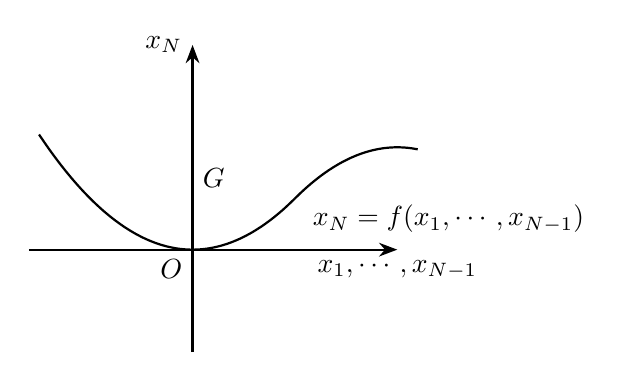
\begin{tikzpicture}[> = Stealth, thick, scale = 1.3]
		\draw [->] (-1.6,0) -- (0,0)node[below left]{$O$} -- (2,0)node[below]{$x_1,\cdots,x_{N-1}$};
		\draw [->] (0,-1) -- (0,0.7)node[right]{$G$} -- (0,2)node[left]{$x_N$};
		\draw[smooth,domain=-1.5:1]plot(\x,0.5*\x*\x);
		\draw[smooth,domain=1:2.2]plot(\x,{-0.5*(\x-2)^2+1});
		\node (a) at (2.5,0.3) {$x_N=f(x_1,\cdots,x_{N-1})$};
	\end{tikzpicture}
	\captionof{figure}{\label{fig5.1}}
\end{minipage}

设$G\subset\MR^N$,对每一个$x\in\partial G$,可以通过平移、旋转把$x$变成坐标原点,并使$G$的边界$\partial G$在$x$处的切平面正好是$x_N=0$.这时在原点附近,$G$可表示为
\[G=\left\{(x_1,\cdots,x_N)\in\MR^N\colon f(x_1,\cdots,x_{N-1})-x_N<0\right\}.\]
$G$在原点附近是欧氏凸域等价于由$f$的二阶导数构成的方阵半正定
\begin{equation}\label{eq5.3.1}
	\left(\pppp{f}{x_j}{x_l}\right)_{1\le j,l\le N-1}\ge0;
\end{equation}

严格凸等价于上述方阵正定
\begin{equation}\label{eq5.3.2}
	\left(\pppp{f}{x_j}{x_l}\right)_{1\le j,l\le N-1}>0.
\end{equation}
如果记$r=f(x_1,\cdots,x_{N-1})-x_N$,因为$f$在原点达到极小,所以$\pp{r}{x_j}\bigg|_{x=0}=\pp{f}{x_j}\bigg|_{x=0}=0,j=1,\cdots,N-1$,但$\pp{r}{x_N}=-1\neq0$,即$r(x_1,\cdots,x_N)=0$在原点处的法向量是$(0,\cdots,0,-1)$,因而切向量是$(\eta_1,\cdots,\eta_{N-1},0)$.由于\eqref{eq5.3.1},\eqref{eq5.3.2}分别为
\[\sum_{j,l=1}^{N-1}\pppp{f}{x_j}{x_l}\eta_j\eta_l=\sum_{j,l=1}^{N-1}\pppp{r}{x_j}{x_l}\eta_j\eta_l\ge0\quad\text{(或$>0$)},\]
又因为$\eta$的第$N$个坐标为$0$,故上式等价于
\[\sum_{j,l=1}^N \pppp{r}{x_j}{x_l}\eta_j\eta_l\ge0\quad\text{(或$>0$)}.\]
因而\eqref{eq5.3.1},\eqref{eq5.3.2}可理解为$N$阶方阵$\left(\pppp{r}{x_j}{x_l}\right)_{1\le j,l\le N}$在原点的切平面半正定或正定.为了能把上面的结果严格地叙述出来,我们引进下面的定义.
\begin{definition}\label{def5.3.1}
	$\MR^N$中的开集$G$在$p\in\partial G$点称为具有$C^k(1\le k\le\infty)$类\textbf{可微边界},如果存在$p$点的邻域$U$和一个实值函数$\varphi\in C^k(U)$,使得
	
	(1)\hypertarget{5.3.1}{}
	$U\cap G=\{x\in U\colon\varphi(x)<0\}$;
	
	(2)\hypertarget{5.3.1}{}
	$\dif\varphi(x)\neq0,x\in U$.
	
	如果$\partial G$上每一点都具有$C^k$类可微边界,就称$G$具有\textbf{$C^k$类可微边界},简称\textbf{$G$具有$C^k$边界}.
	
	任何满足\hyperlink{5.3.1}{(1)}、\hyperlink{5.3.1}{(2)}的函数$\varphi\in C^k(U)$称为$G$在$p$点的\textbf{局部定义函数}\index{J!局部定义函数}.如果$U$是$\partial G$的邻域,那么满足\hyperlink{5.3.1}{(1)}、\hyperlink{5.3.1}{(2)}的函数$\varphi\in C^k(U)$称为$G$的\textbf{整体定义函数},简称$G$的\textbf{定义函数}\index{D!定义函数}.
\end{definition}
例如$\varphi(z)=z\bar{z}'-1$便是单位球的定义函数.

容易看出,从定义\ref{def5.3.1}的\hyperlink{5.3.1}{(1)} \hyperlink{5.3.1}{(2)}即可推出
\[U\cap\partial G=\{x\in U\colon\varphi(x)=0\},\]
\[U\setminus\bar{G}=\{x\in U\colon\varphi(x)>0\}.\]
对于有界域,一定有整体定义函数.
\begin{prop}\label{prop5.3.2}
	设$G$是$\MR^N$中具有$C^k$边界的有界域,则必存在$G$的整体定义函数,即存在$\partial G$的邻域$U$和$\varphi\in C^k(U)$,使得
	\[G\cap U=\{x\in U\colon\varphi(x)<0\}.\]
\end{prop}
\begin{proof}
	由于$\partial G$是紧的,故存在有限多个开集$U_1,\cdots,U_m$和局部定义函数$\varphi_j\in C^k(U_j)$,\\
	$j=1,\cdots,m$,使得$\partial G\subset\bigcup\limits_{j=1}^m U_j$.记$U=\bigcup\limits_{j=1}^m U_j$.由单位分解定理\ref{thm4.6.3},存在$f_j\in C_0^\infty(U_j),0\le f_j\le1$,在$U$上有$\sum\limits_{j=1}^m f_j(x)=1$.现在定义
	\[\varphi=\sum_{j=1}^{m}f_j\varphi_j,\]
	那么$\varphi\in C^k(\MR^N)$.现任取$x\in\partial G$,则必存在某个$l$,使得$x\in U_l$.对于其它$U_j,j\neq l$,有两种情形:如果$x\notin U_j$,则因$\supp f_j\subset U_j$,所以$f_j(x)=0$;如果$x\in U_j$,则$\varphi_j(x)=0$,因而总有$\varphi(x)=0$.同样道理$\dif\varphi(x)\neq0$.适当收缩$U$,即可断言对所有$x\in U,\dif\varphi(x)\neq0$.最后来证明
	\[U\cap G=\{x\in U\colon\varphi(x)<0\}.\]
	事实上,如果$x\in U\cap G$,则必存在某个$l$,使得$x\in U_l\cap G$,和上面一样讨论,即可得$\varphi(x)\le f_l(x)\varphi_l(x)$.反之,如果对某点$x\in U$,有$\varphi(x)<0$,则从$\varphi$的定义知道,必有某个$j$,使得$\varphi_j(x)<0$,因而$x\in U_j\cap G\subset U\cap G$.
\end{proof}
现在给出$\partial G$某点处切空间的定义.

设$G\subset\MR^N$具有$C^1$边界,$\varphi$是$G$的定义函数,$p\in\partial G$,我们称
\[T_p(\partial G)=\left\{\xi\in\MR^N\colon\sum_{j=1}^N \pp{\varphi}{x_j}(p)\xi_j=0\right\}\]
为$\partial G$在$p$点处的\textbf{切空间}\index{Q!切空间}\index[symbolindex]{\textbf{点集}!$T_p(\partial G)$}.
现在可以把刚才讨论的结果表述为:

设$G$是$\MR^N$中具有$C^2$边界的有界域\index{C!$C^2$边界},$\varphi$是它的定义函数,那么$G$是欧氏凸域的充分必要条件是
\begin{equation}\label{eq5.3.3}
	\sum_{j,k=1}^{N}\pppp{\varphi}{x_j}{x_k}(p)\xi_j\xi_k\ge0
\end{equation}
对所有$p\in\partial G$和$\xi\in T_p(\partial G)$成立.

如果下式成立
\[\sum_{j,k=1}^{N}\pppp{\varphi}{x_j}{x_k}(p)\xi_j\xi_k>0,\quad \xi\in T_p(\partial G),\quad \xi\neq0,\]
就说$G\subset\MR^N$在$p\in\partial G$是强欧氏凸的.如果$G$在$\partial G$的每点都是强欧氏凸的,就说$G$是强欧氏凸域.
\subsection{Levi拟凸域和强拟凸域}
1910年,E. E. Levi发现具有$C^2$边界的全纯域,它的定义函数也满足一个类似于\eqref{eq5.3.3}的条件(在复的形式下).由于欧氏凸域在双全纯映射下不再是欧氏凸域(这一点从单复变的Riemann共形映射存在定理即可看出),而全纯域在双全纯映射下还是全纯域.为了要得到Levi的条件,我们应该研究一下\eqref{eq5.3.3}的哪部分在双全纯映射下不变.

条件\eqref{eq5.3.3}是说由定义函数$\varphi$的二阶偏导数构成的二次型在切空间$T_p(\partial G)$上是半正定的.在复的形式下,切空间$T_p(\partial G)$应该由复切空间来代替.我们知道,$\MC^n$中的点$z=(z_1,\cdots,z_n)$也可看成$\MR^{2n}$中的点
\[z=(x_1,y_1,\cdots,x_n,y_n),\]
这里$z_j=x_j+\ii y_j$.因此$\ii z$作为$\MR^{2n}$中的点,它的坐标是
\[\ii z=(-y_1,x_1,\cdots,-y_n,x_n).\]
设$w=(w_1,\cdots,w_n)$是$\MC^n$中另一个点,$w_j=u_j+\ii v_j$.作为$\MC^n$中的向量,$z,w$正交是指
\[\langle z,w\rangle=\sum_{j=1}^{n}z_j\bar{w}_j=0.\]
作为$\MR^{2n}$中的向量,$z,w$正交是指
\[z\cdot w=\sum_{j=1}^{n}(x_ju_j+y_jv_j)=0.\]
容易看出$\langle z,w\rangle$和$z\cdot w$有下面的关系:
\begin{equation}\label{eq5.3.4}
	z\cdot w=\Re\langle z,w\rangle,\quad -\ii z\cdot w=\Im\langle z,w\rangle.
\end{equation}
设$w$是$\MC^n$中一个给定的向量,从\eqref{eq5.3.4}可以看出,$z$和$w$复正交,即$\langle z,w\rangle=0$的充分必要条件是
\[z\cdot w=0,\,-\ii z\cdot w=0.\]
如果记$-\ii z=z'$,则$z'$和$w$实正交,而$z=\ii z'$.因此,$z$和$w$复正交的充分必要条件是$z$和$w$实正交,而且$z=\ii z',z'$是一个与$w$实正交的向量.由此,我们给出复切空间的定义如下:
\begin{definition}\label{def5.3.3}
	设$G\subset\MC^n$具有$C^1$边界,称
	\[T_p^\MC(\partial G)=T_p(\partial G)\cap\ii T_p(\partial G)\]
	为$\partial G$在$p$点的\textbf{复切空间}\index{F!复切空间}\index[symbolindex]{\textbf{点集}!$T_p^\MC(\partial G)$}.
\end{definition}
\begin{prop}\label{prop5.3.4}
	设$\varphi$是$G\subset\MC^n$在$p\in\partial G$处的局部定义函数,那么
	\[T_p^\MC(\partial G)=\left\{w\in\MC^n\colon\sum_{j=1}^{n}\pp{\varphi}{z_j}(p)w_j=0\right\}.\]
\end{prop}
\begin{proof}
	因为$\pp{}{z_j}=\frac12\left(\pp{}{x_j}-\ii\pp{}{y_j}\right),w_j=u_j+\ii v_j$,所以$\sum\limits_{j=1}^n \pp{\varphi}{z_j}(p)w_j=0$的充分必要条件是
	\[\sum_{j=1}^{n}\left(\pp{\varphi}{x_j}(p)u_j+\pp{\varphi}{y_j}(p)v_j\right)=0,\]
	\[\sum_{j=1}^{n}\left(\pp{\varphi}{x_j}(p)v_j-\pp{\varphi}{y_j}(p)u_j\right)=0.\]
	前者说明$w\in T_p(\partial G)$,后者说明$-\ii w\in T_p(\partial G)$,即$w\in\ii T_p(\partial G)$.
\end{proof}
现在把\eqref{eq5.3.3}中的二次型用复的形式来表示.

记$w_j=\xi_j+\ii\eta_j$,把$w=(\xi_1,\eta_1,\cdots,\xi_n,\eta_n)$看成$\MR^{2n}$中的点.注意到
\[\pp{}{x_j}=\pp{}{z_j}+\pp{}{\bar{z}_j},\quad \pp{}{y_j}=\frac1{\ii}\left(\pp{}{\bar{z}_j}-\pp{}{z_j}\right),\]
\[\xi_j=\frac12(w_j+\bar{w}_j),\quad \eta_j=\frac1{2\ii}(w_j-\bar{w}_j),\]
那么\eqref{eq5.3.3}中的二次型可以写为
\begin{align*}
	&\sum_{j,k=1}^{n}\pppp{\varphi}{x_j}{x_k}(p)\xi_j\xi_k+2\sum_{j,k=1}^{n}\pppp{\varphi}{x_j}{y_k}(p)\xi_j\eta_k+\sum_{j,k=1}^{n}\pppp{\varphi}{y_j}{y_k}(p)\eta_j\eta_k\\
	=&\frac14\sum_{j,k=1}^{n}\left(\pp{}{z_j}+\pp{}{\bar{z}_j}\right)\left(\pp{}{z_k}+\pp{}{\bar{z}_k}\right)\varphi(p)(w_j+\bar{w}_j)(w_k+\bar{w}_k)+\\
	&\frac12\sum_{j,k=1}^{n}\left(\pp{}{z_j}+\pp{}{\bar{z}_j}\right)\frac1{\ii}\left(\pp{}{\bar{z}_k}-\pp{}{z_k}\right)\varphi(p)(w_j+\bar{w}_j)\frac1{\ii}(w_k-\bar{w}_k)+\\
	&\frac14\sum_{j,k=1}^{n}\frac1{\ii}\left(\pp{}{\bar{z}_j}-\pp{}{z_j}\right)\frac1{\ii}\left(\pp{}{\bar{z}_k}-\pp{}{z_k}\right)\varphi(p)\cdot\\
	&\frac1{\ii}(w_j-\bar{w}_j)\frac1{\ii}(w_k-\bar{w}_k)\\
	=&2\Re\left\{\sum_{j,k=1}^{n}\pppp{\varphi}{z_j}{z_k}(p)w_jw_k\right\}+2\sum_{j,k=1}^{n}\pppp{\varphi}{z_j}{\bar{z}_k}(p)w_j\bar{w}_k.
\end{align*}
如果记\index[symbolindex]{\textbf{函数和映射}!$Q_p(\varphi$,$w)$}\index[symbolindex]{\textbf{函数和映射}!$L_p(\varphi$,$w)$}
\[Q_p(\varphi,w)=\sum_{j,k=1}^{n}\pppp{\varphi}{z_j}{z_k}(p)w_jw_k,\]
\begin{equation}\label{eq5.3.5}
	L_p(\varphi,w)=\sum_{j,k=1}^{n}\pppp{\varphi}{z_j}{\bar{z}_k}(p)w_j\bar{w}_k,
\end{equation}
那么\eqref{eq5.3.3}中的二次型即为
\[2\Re Q_p(\varphi,w)+2L_p(\varphi,w).\]
因此,$G$是欧氏凸域的条件可用复的形式表示为
\begin{equation}\label{eq5.3.6}
	\Re Q_p(\varphi,w)+L_p(\varphi,w)\ge0,\quad w\in T_p(\partial G).
\end{equation}
注意到
\[Q_p(\varphi,-\ii w)=-Q_p(\varphi,w),\quad L_p(\varphi,-\ii w)=L_p(\varphi,w).\]
在\eqref{eq5.3.6}中用$-\ii w$代$w$,即得
\begin{equation}\label{eq5.3.7}
	-\Re Q_p(\varphi,w)+L_p(\varphi,w)\ge0,\quad -\ii w\in T_p(\partial G).
\end{equation}
\eqref{eq5.3.6},\eqref{eq5.3.7}两式相加即得
\begin{equation}\label{eq5.3.8}
	L_p(\varphi,w)\ge0,\quad w\in T_p^\MC(\partial G).
\end{equation}
这就是Levi得到的条件.稍后我们将证明这个条件在双全纯映射下是不变的.现在就用条件\eqref{eq5.3.8}来定义一类新的域.通常称\eqref{eq5.3.8}为\textbf{Levi条件}\index{L!Levi条件}.
\begin{definition}\label{def5.3.5}
	如果Levi条件\eqref{eq5.3.8}对$\MC^n$中具有$C^2$边界的域$G$的某个在$p$点附近的局部定义函数$\varphi$成立,称$G$在$p\in\partial G$是\textbf{Levi拟凸的}.如果Levi条件\eqref{eq5.3.8}对所有$p\in\partial G$成立,称$G$是\textbf{Levi拟凸域}\index{Y!域!Levi拟凸域}.
\end{definition}
\begin{definition}\label{def5.3.6}
	设$G$是$\MC^n$中具有$C^2$边界的域,如果$L_p(\varphi,w)>0$对所有$w\in T_p^\MC(\partial G),w\neq0$成立,称$G$在$p\in\partial G$是\textbf{强Levi拟凸的}.如果$G$在每点$p\in\partial G$都是强Levi拟凸的,称$G$是\textbf{强Levi拟凸域}\index{Y!域!强Levi拟凸域}.
\end{definition}
由\eqref{eq5.3.5}式定义的$L_p(\varphi,w)$称为\textbf{Levi形式}\index{L!Levi形式}或定义函数$\varphi$在$p$点的\textbf{复Hessian}\index{F!复Hessian}.

从上面的讨论,我们已经得到
\begin{theorem}\label{thm5.3.7}
	$\MC^n$中具有$C^2$边界的欧氏凸域是Levi拟凸域.
\end{theorem}
定理\ref{thm5.3.7}的逆是不成立的.

下面看几个例子.
\begin{example}\label{exa5.3.8}
单位球$B_n$是强Levi拟凸域.	
\end{example}
\begin{proof}
	因为它的定义函数$\varphi(z)=z\bar{z}'-1,\pp{\varphi}{z_j}=\bar{z}_j,\pppp{\varphi}{z_j}{\bar{z}_k}=\delta_{jk}$,所以
	\[\sum_{j,k=1}^{n}\pppp{\varphi}{z_j}{\bar{z}_k}w_j\bar{w}_k=\sum_{j,k=1}^{n}\delta_{jk}w_j\bar{w}_k=\sum_{j=1}^{n}|w_j|^2>0,w\neq0.\]
	因而$B_n$是强Levi拟凸域.
\end{proof}
\begin{example}\label{exa5.3.9}
	域$G=\{z\in\MC^n\colon|z_1|^{p_1}+\cdots+|z_n|^{p_n}<1,p_j\ge2,j=1,\cdots,n\}$是Levi拟凸域.只有当$p_1=\cdots=p_n=2$时,它是强Levi拟凸域.
\end{example}
\begin{proof}
	$G$的定义函数是
	\[\varphi(z)=\left(z_1\bar{z}_1\right)^{\frac{p_1}2}+\cdots+\left(z_n\bar{z}_n\right)^{\frac{p_n}2}-1.\]
	直接计算可得
	\[\pp{\varphi}{z_j}=\frac{p_j}{2}\left(z_j\bar{z}_j\right)^{\frac{p_j}{2}-1}\bar{z}_j,\quad 
	\pppp{\varphi}{z_j}{\bar{z}_k}=\frac{p_j^2}{4}|z_j|^{p_j-2}\delta_{jk}.\]
	因而
	\begin{equation}\label{eq5.3.9}
		\sum_{j,k=1}^{n}\pppp{\varphi(\zeta)}{z_j}{\bar{z}_k}w_j\bar{w}_k=\frac14\sum_{j=1}^{n}p_j^2 |\zeta_j|^{p_j-2}|w_j|^2\ge0.	\end{equation}
	因而$G$是Levi拟凸域.如果有某个$p_l>2$,这时取$\zeta\in\partial G$,要求它的第$l$个坐标$\zeta_l=0$,取$w=(0,\cdots,1,\cdots,0)$,它的第$l$个坐标为$1$,其它坐标为$0$,则$w\in T_\zeta^\MC(\partial G)$,且\eqref{eq5.3.9}的左端为$0$.因此$G$在这种点上不是强拟凸域.但当$p_j=2,j=1,\cdots,n$时,这种情况不会发生,这时$G$就是单位球.
\end{proof}
\begin{example}\label{exa5.3.10}
	当$p_j\ge1(j=1,\cdots,n)$时,例\ref{exa5.3.9}中的域$G$是欧氏凸域.
\end{example}
\begin{proof}
	我们用欧氏凸域的几何定义来证.我们证明,如果$a\in G,b\in G$,那么$\frac{a+b}{2}$也属于$G$.事实上,记
	\[\varphi(z)=\sum_{j=1}^{n}|z_j|^{p_j}-1,\]
	则$\varphi(a)<0,\varphi(b)<0$.利用不等式
	\[(t_1+t_2)^p \le 2^{p-1}(t_1^p+t_2^p),\quad t_1\ge0,t_2\ge0,p\ge1.\]
	即得
	\begin{align*}
		\varphi\left(\frac{a+b}{2}\right)
		&=\sum_{j=1}^{n}\left|\frac{a_j+b_j}{2}\right|^{p_j}-1\le\sum_{j=1}^{n}\frac{1}{2^{p_j}}\left(|a_j|+|b_j|\right)^{p_j}-1\\
		&\le\frac12\sum_{j=1}^{n}\left(|a_j|^{p_j}+|b_j|^{p_j}\right)-1<0.
	\end{align*}
因而$G$是欧氏凸域.
\end{proof}
这个例子说明欧氏凸域不一定是强Levi拟凸域.
\subsection{Levi拟凸性和域的定义函数无关\index{D!定义函数!域的定义函数}}
在上面的Levi拟凸域和强Levi拟凸域的定义中,存在一个明显的问题,那就是定义函数的不唯一性.
如果在$\varphi$作为定义函数时,$G$是Levi拟凸域,换了另一个定义函数,它是否还是Levi拟凸域?下面我们将证明,域的Levi拟凸性或强Levi拟凸性与定义函数的选取无关.为此先证明
\begin{prop}\label{prop5.3.11}
	设$G$是$\MC^n$中的域,$p\in\partial G,U$是$p$的邻域.如果$\varphi$和$\psi$是$G$的两个在$U$上的$C^k$类局部定义函数,那么存在$p$的邻域$V\subset U$和唯一的正函数$h\in C^{k-1}(V)$,使得
	\[\varphi=h\psi\]
	在$V$上成立.
\end{prop}
\begin{proof}
	因为$p\in U\cap\partial G$,所以$\varphi(p)=0$.由于$\dif\varphi(p)\neq0$,不妨设$\pp{\varphi}{x_1}(p)\neq0$.根据隐函数存在定理,存在$p$的邻域$V$,使得在$V$上可以从$\varphi(x_1,\cdots,x_n,y_1,\cdots,y_n)=0$中解出
	\[x_1=\sigma(x_2,\cdots,x_n,y_1,\cdots,y_n).\]
	不妨设$\varphi<0$对应于$x_1<\sigma(x_2,\cdots,x_n,y_1,\cdots,y_n)$.作变换
	\[\Phi\colon(x_1,\cdots,x_n,y_1,\cdots,y_n)\to(u_1,\cdots,u_n,v_1,\cdots,v_n)\]
	如下
	\[u_1=x_1-\sigma(x_2,\cdots,x_n,y_1,\cdots,y_n),\]
	\[u_j=x_j-p_j,\quad j=2,\cdots,n.\]
	\[v_j=y_j-p_{n+j},\quad j=1,\cdots,n.\]
	这里$(p_1,\cdots,p_{2n})$是$p$在$\MR^{2n}$中的坐标.记$\Phi(V)=Q$,命
	\[\widetilde{\varphi}=\varphi\circ\Phi^{-1},\quad \widetilde{\psi}=\psi\circ\Phi^{-1},\]
	则$\widetilde{\varphi}$和$\widetilde{\psi}$是$Q$上的$C^k$类函数.由于$\Phi(p)=0$,故$Q$是原点的邻域.不妨假定$Q$是欧氏凸的,不然的话,作一个以原点为中心包含在$Q$中的小球即行.命
	\[h_1(u_1,\cdots,u_n,v_1,\cdots,v_n)=\int_{0}^{1}\pp{\widetilde{\varphi}}{u_1}(tu_1,u_2,\cdots,u_n,v_1,\cdots,v_n)\dif t,\]
	\[h_2(u_1,\cdots,u_n,v_1,\cdots,v_n)=\int_{0}^{1}\pp{\widetilde{\psi}}{u_1}(tu_1,u_2,\cdots,u_n,v_1,\cdots,v_n)\dif t.\]
	因为$Q$是欧氏凸域,上述积分有意义,且$h_1,h_2\in C^{k-1}(Q)$.因为$\pp{\widetilde{\varphi}}{u_1}=\pp{\varphi}{x_1}\neq0,\pp{\widetilde{\psi}}{u_1}=\pp{\psi}{x_1}\neq0$(因为$\dif\psi\neq0$,故可假设$\pp{\psi}{x_1}\neq0$),所以$h_1\neq0,h_2\neq0$.由于$\widetilde{\varphi}(0,u_2,\cdots,v_n)=\varphi\circ\Phi^{-1}(0,u_2,\cdots,v_n)=0$,因而
	\begin{align*}
		h_1(u_1,\cdots,v_n)
		&=\frac1{u_1}\left(\widetilde{\varphi}(u_1,\cdots,v_n)-\widetilde{\varphi}(0,u_2,\cdots,v_n)\right)\\
		&=\frac1{u_1}\widetilde{\varphi}(u_1,\cdots,v_n).
	\end{align*}
故得$h_1u_1=\widetilde{\varphi}$,同理$h_2u_1=\widetilde{\psi}$在$Q$上成立.命$\widetilde{h}=\frac{h_1}{h_2}$,则$\widetilde{h}\in C^{k-1}(Q)$.命$h=\widetilde{h}\circ\Phi$,则$h\in C^{k-1}(V)$.且当$z\in V$时,有
\begin{align*}
	h(z)\psi(z)
	&=\widetilde{h}(\Phi(z))\widetilde{\psi}(\Phi(z))=\frac{h_1(\Phi(z))}{h_2(\Phi(z))}\widetilde{\psi}(\Phi(z))\\
	&=h_1(\Phi(z))u_1=\widetilde{\varphi}(\Phi(z))=\varphi(z).
\end{align*}
$h$的唯一性由上面的等式即明.由于$\varphi$和$\psi$在$G\cap U$中都取负值,在$(\MC^n\setminus G)\cap U$中都取正值,所以$h$在$G\cap U$和$(\MC^n\setminus G)\cap U$中取正值.至于在$\partial G$上,由于$\dif\varphi=h\dif\psi+\psi\dif h=h\dif\psi$,且因$\dif\varphi\neq0,\dif\psi\neq0$,所以$h\neq0$.而已知$h$在$G$内取正值,故在$\partial G$上也取正值.
\end{proof}
有了这个命题就可证明下面的
\begin{prop}\label{prop5.3.12}
	设$G$是$\MC^n$中的域,$p\in\partial G,U$是$p$的邻域.如果$\varphi$和$\psi$是$G$的两个在$U$上的$C^2$定义函数,那么
	
	(1)\hypertarget{5.3.12}{}
	由$\varphi$和$\psi$产生的$p$点处的复切空间是相同的;
	
	(2)\hypertarget{5.3.12}{}
	如果$\varphi$满足Levi条件\eqref{eq5.3.8}。那么$\psi$也满足.
\end{prop}
\begin{proof}
	\hyperlink{5.3.12}{(1)}
	由命题\ref{prop5.3.11},存在$p$的邻域$V\subset U$及正函数$h\in C^1(V)$,使得$\varphi=h\psi$在$V$上成立.于是
	\begin{equation}\label{eq5.3.10}
		\pp{\varphi}{z_j}=\pp{h}{z_j}\psi+h\pp{\psi}{z_j}.
	\end{equation}
由于$\psi(p)=0$,所以
\[\sum_{j=1}^{n}\pp{\varphi}{z_j}(p)w_j=h(p)\sum_{j=1}^{n}\pp{\psi}{z_j}(p)w_j.\]
由命题\ref{prop5.3.4},即知二者产生的复切空间$T_p^\MC(\partial G)$是相同的.
	
	\hyperlink{5.3.12}{(2)}
	在证明第二个结论时,我们需要如下的一个简单事实.设$f,g$是定义在$a\in\MR^N$附近的两个函数,$g(a)=0,\pp{g}{x_j}(a)$存在,$f$在$a$处连续,那么$fg$在$a$处对$x_j$的偏导数存在,而且
	\[\pp{(fg)}{x_j}(a)=f(a)\pp{g}{x_j}(a).\]
	
	现在让\eqref{eq5.3.10}的两端对$\bar{z}_k$求偏导数,并在$p$处连续,$\psi(p)=0$,因而应用上面的简单事实可得
	\[\pp{}{\bar{z}_k}\left(\pp{h}{z_j}\psi\right)(p)=\pp{h}{z_j}(p)\pp{\psi}{\bar{z}_k}(p).\]
	\eqref{eq5.3.10}右端第二项求导的结果是
	\[\pp{}{\bar{z}_k}\left(h\pp{\psi}{z_j}\right)(p)=\pp{h}{\bar{z}_k}(p)\pp{\psi}{z_j}(p)+h(p)\pppp{\psi}{z_j}{\bar{z}_k}(p).\]
	于是由\eqref{eq5.3.10}即得
	\begin{align*}
		\sum_{j,k=1}^{n}\pppp{\varphi}{z_j}{\bar{z}_k}(p)w_j\bar{w}_k
		=&2\Re\left\{\sum_{k=1}^{n}\pp{h}{\bar{z}_k}(p)\bar{w}_k\sum_{j=1}^{n}\pp{\psi}{z_j}(p)w_j\right\}+\\
		&h(p)\sum_{j,k=1}^{n}\pppp{\psi}{z_j}{\bar{z}_k}(p)w_j\bar{w}_k.
	\end{align*}
因而当$w\in T_p^\MC(\partial G)$时,就有
\[L_p(\varphi,w)=h(p)L_p(\psi,w).\]
因为$h(p)>0$,故$L_p(\varphi,w)$和$L_p(\psi,w)$同时取正值.
\end{proof}
这个命题说明域的Levi拟凸性或强拟凸性与定义函数的选取无关.但从证明中可以看出,如果$w$不是取自复切空间$T_p^\MC(\partial G)$,Levi形式的符号有可能随定义函数而异.但在强Levi拟凸的情形,我们总可以选取一个适当的定义函数,使其Levi形式对任意$w\neq0$都取正值.
\begin{theorem}\label{thm5.3.13}
	设$G$是$\MC^n$中具有$C^2$边界的有界强Levi拟凸域,则必存在$G$的定义函数$\rho$和正数$\lambda_0$,使得对任意非零的$w\in\MC^n$和$p\in\partial G$,有
	\begin{equation}\label{eq5.3.11}
		L_p(\rho,w)\ge\lambda_0|w|^2.
	\end{equation}
\end{theorem}
\begin{proof}
	根据命题\ref{prop5.3.2},设$\varphi$是$G$的一个整体定义函数,则对任意$\alpha>0,\rho=\frac1\alpha (\ee^{\alpha\varphi}-1)$也是$G$的一个定义函数.由直接计算可得
	\[\pppp{\rho}{z_j}{\bar{z}_k}=\alpha\ee^{\alpha\varphi}\pp{\varphi}{z_j}\pp{\varphi}{\bar{z}_k}+\ee^{\alpha\varphi}\pppp{\varphi}{z_j}{\bar{z}_k}.\]
	固定$p\in\partial G$,则$\varphi(p)=0$,由上式可得
	\begin{equation}\label{eq5.3.12}
		L_p(\rho,w)=\left\{L_p(\varphi,w)+\alpha\left|\sum_{j=1}^{n}\pp{\varphi}{z_j}(p)w_j\right|^2\right\}\ee^{\alpha\varphi}.
	\end{equation}
用$S$记$\MC^n$中的单位球面,命
\[A=\{w\in S\colon L_p(\varphi,w)\le0\}.\]
由于$G$是强Levi拟凸域,且$A$是紧的,所以
\[\min_{w\in A}\left|\sum_{j=1}^{n}\pp{\varphi}{z_j}(p)w_j\right|>0.\]
于是必可取到正数$\alpha$,使得
\[\alpha>-\min_{w\in A} L_p(\varphi,w)\left(\min_{w\in A}\left|\sum_{j=1}^{n}\pp{\varphi}{z_j}(p)w_j\right|\right)^{-2}.\]
由\eqref{eq5.3.12}知道,这样选取的$\alpha$所产生的$\rho$必有
\begin{equation}\label{eq5.3.13}
	L_p(\rho,w)>0
\end{equation}
对任意$w\in S$成立.由$L_p(\rho,w)$的连续性,\eqref{eq5.3.13}对$p$附近的点也成立.综上所述,对每个$p\in\partial G$,存在$p$的邻域$U(p)$及相应的$\alpha>0$,使得\eqref{eq5.3.13}对$U(p)$中的点都成立.由于$\partial G$是紧的,故可取到有限个$U(p)$覆盖$\partial G$,每个$U(p)$对应一个$\alpha$,设$\alpha_0$是这有限个$\alpha$中之最大者.取$\rho=\frac1{\alpha_0}(\ee^{\alpha_0\varphi}-1)$,则\eqref{eq5.3.13}对所有$p\in\partial G$成立.由于$\partial G\times S$是紧的,$L_p(\rho,w)$在$\partial G\times S$上有最小值$\lambda_0>0$,因而对任意非零的$w\in\MC^n$及$p\in\partial G$,\eqref{eq5.3.11}成立.
\end{proof}
最后,我们来证明Levi拟凸性在双全纯映射下的不变性.
\begin{prop}\label{prop5.3.14}
	设$\MC^n$中的域$G$在$p\in\partial G$附近具有$C^2$边界,$U$是$p$的一个邻域.如果$\zeta=F(z)$是$U$上一个双全纯映射,记$D=F(U\cap G)$,那么$D$在$q=F(p)$处是Levi拟凸的充分必要条件是$G$在$p$处是Levi拟凸的.
\end{prop}
\begin{proof}
	设$\varphi$是$G$在$p$附近的定义函数,那么$\psi=\varphi\circ F^{-1}$是$D$在$q$附近的定义函数.用$F'(p)$记双全纯映射$F$在$p$点处的导数,若记$\xi=F'(p)w$,那么从$\varphi(z)=\psi(F(z))$通过直接计算可得
	\begin{equation}\label{eq5.3.14}
		\sum_{j=1}^{n}\pp{\varphi}{z_j}(p)w_j=\sum_{j=1}^{n}\pp{\psi}{\zeta_j}(q)\xi_j,
	\end{equation}
\begin{equation}\label{eq5.3.15}
	L_p(\varphi,w)=L_q(\psi,\xi).
\end{equation}
若$G$在$p$处是Levi拟凸的,取$\xi\in T_q^\MC(\partial D)$,记$w=(F'(p))^{-1}\xi$,则从\eqref{eq5.3.14}知道$w\in T_p^\MC(\partial G)$,因而$L_p(\varphi,w)\ge0$,从\eqref{eq5.3.15}即得$L_q(\psi,\xi)\ge0$,因而$D$在$q$处是Levi拟凸的.反之亦然.
\end{proof}
\section{多重次调和函数\label{sec5.4}}
\subsection{多重次调和函数的基本性质}
在下面的讨论中,多重次调和函数的概念起着重要的作用.
\begin{definition}\label{def5.4.1}
	设$G$是$\MC^n$中的域,$u$是$G$上的实值函数$u\colon G\to\MR\cup\{-\infty\}(u\not\equiv-\infty)$.如果$u$满足
	
	(1)\hypertarget{5.4.1}{}
	$u$是上半连续的;
	
	(2)\hypertarget{5.4.1}{}
	限制在每条复直线上的$u$都是次调和的,即对每个$z_0\in G$与$a\in\MC^n,u$是$\{z_0+\lambda a\colon\lambda\in\MC\}\cap G$上的单复变数$\lambda$的次调和函数;
	
	就称$u$是$G$上的\textbf{多重次调和函数}\index{D!多重次调和函数}.用$PS(G)$记$G$上多重次调和函数的全体\index[symbolindex]{\textbf{函数和映射}!$PS(G)$}.
\end{definition}
称$\{z_0+\lambda a\colon\lambda\in\MC\}$是通过$z_0$的以$a$为方向的\textbf{复直线}.

如果$f\in H(G)$,那么$f(z_0+\lambda a)$是$\lambda$的全纯函数.由命题\ref{prop1.5.7}知道$\log|f|$和$|f|^p(0<p<\infty)$都是$G$上的多重次调和函数.
\begin{prop}\label{prop5.4.2}
	域$G$上的多重次调和函数一定是次调和函数.
\end{prop}
\begin{proof}
	设$u$是$G$上的多重次调和函数.任取$z_0+rB\subset G$,因为$u(z_0+\lambda\zeta)$是$\lambda$的次调和函数,这里$\zeta\in\partial B$,所以$u(z_0)\le\frac1{2\pi}\int_{-\pi}^{\pi}u(z_0+r\ee^{\ii\theta}\zeta)\dif\theta$,两边对$\zeta$在$\partial B$上积分,利用定理\ref{thm1.4.4}\hyperlink{1.4.4}{(1)}得
	\[u(z_0)\le\int_{\partial B}\dif\sigma(\zeta)\frac1{2\pi}\int_{-\pi}^{\pi}u(z_0+r\ee^{\ii\theta}\zeta)\dif\theta=\int_{\partial B}u(z_0+r\zeta)\dif\sigma(\zeta).\]
	由定义\ref{def1.5.9}知道$u$是$G$上的次调和函数.
\end{proof}
\begin{prop}\label{prop5.4.3}
	如果$u$是域$G\subset\MC^n$上的二次连续可微函数,那么$u$在$G$上是多重次调和函数的充分必要条件是$\left(\pppp{u}{z_j}{\bar{z}_l}\right)_{1\le j,l\le n}\ge0$在$G$上成立.
\end{prop}
\begin{proof}
	对于任何复直线$z_0+\lambda a\subset G,a\in\MC^n$,由定理\ref{thm1.5.8}知道,函数$\lambda\to u(z_0+\lambda a)$是次调和函数的充分必要条件是$\pppp{u(z_0+\lambda a)}{\lambda}{\bar{\lambda}}\ge0$,即$\sum\limits_{j,l=1}^n \pppp{u}{z_j}{\bar{z}_l}a_j\bar{a}_l\ge0$,它等价于$\left(\pppp{u}{z_j}{\bar{z}_l}\right)_{1\le j,l\le n}\ge0$.
\end{proof}
上面的条件也可以等价地说成$u$的Levi形式
\[L_p(u,w)\ge0\]
对所有$p\in G$及$w\in\MC^n$成立.
\begin{definition}\label{def5.4.4}
	设$G$是$\MC^n$中的域.如果实值函数$u\in C^2(G)$对$p\in G$及所有$w\in\MC^n(w\neq0)$满足$L_p(u,w)>0$,就称$u$在$p$点是\textbf{强多重次调和的}.如果$u$在$G$中所有点都是强多重次调和的,就称$u$在$G$上是\textbf{强多重次调和函数}\index{D!多重次调和函数!强多重次调和函数}.
\end{definition}
例如$u(z)=|z|^2$就是$\MC^n$中的强多重次调和函数.因为$u(z)=\sum_{j=1}^{n}z_j\bar{z}_j,\pppp{u}{z_j}{\bar{z}_k}=\delta_{jk}$,所以$L_p(u,w)=|w|^2>0,w\neq0$对所有$p,w\in\MC^n$成立.

利用强多重次调和函数的概念,定理\ref{thm5.3.13}可叙述为
\begin{theorem}\label{thm5.4.5}
	设$G$是$\MC^n$中具有$C^2$边界的有界强Levi拟凸域,则在$\partial G$的邻域$U$上存在$G$的定义函数$\rho$,使得$\rho$在$U$中是强多次调和函数.
\end{theorem}
利用命题\ref{prop5.4.3},可以证明多重次调和函数在全纯映射下是不变的.
\begin{prop}\label{prop5.4.6}
	设$G,D$分别是$\MC^n$和$\MC^m$中的域,$F\colon D\to G$是全纯映射.如果$u\in PS(G)\cap C^2(G)$,那么$u\circ F\in PS(D)$.
\end{prop}
\begin{proof}
	通过直接计算知道,对任意$a\in D$有
	\[L_a(u\circ F,w)=L_{F(a)}(u,F'(a)w).\]
	因为$u\in PS(G)$,故右端非负,因而左端也非负,所以$u\circ F\in PS(D)$.
\end{proof}
这个命题的缺陷是要假定$u\in C^2(G)$.实际上,,没有这个条件结论也成立,但需要用到关于多重次调和函数的逼近定理.为此先证一个引理.
\begin{lemma}\label{lem5.4.7}
	设$G$是$\MC^n$中的域.如果$u\in PS(G)$,那么$u\in L^1(G,\loc)$\footnote{$L^1(G,\loc)$是指在$G$的任意紧集上可积函数的全体.}\index[symbolindex]{\textbf{函数和映射}!$L^1(G$,$\loc)$}.特别$\{z\in G\colon u(z)=-\infty\}$的Lebesgue测度为$0$.
\end{lemma}
\begin{proof}
	因为$u\not\equiv-\infty$,所以存在$a\in G,u(a)>-\infty$.取$B(a,r)\subset G$,我们证明$\int_{B(a,r)}u\dif\nu$存在.因为$u$在$B(a,r)$中有上界,所以只须证明$\int_{B(a,r)}u\dif\nu>-\infty$.由命题\ref{prop5.4.2}知道,$u$是次调和函数,再根据命题\ref{prop1.5.10},即得
	\[-\infty<u(a)<\int_{B(a,r)}u\dif\nu.\]
	现设
	\[E=\{a\in G\colon\text{$u$在$a$的某个邻域中可积}\}.\]
	显然$E$是开集.由刚才的证明知道$E$不空.今若$a\in G\setminus E$,则由上所证,必有$a$的某个邻域,对这邻域中所有的$z,u(z)=-\infty$.因而$G\setminus E$也是开集.由于$G$是连通的,所以$G=E$.
\end{proof}
\subsection{用$C^\infty$的强多重次调和函数逼近多重次调和函数}
现在可以证明下面的多重次调和函数逼近定理.
\begin{theorem}\label{thm5.4.8}
	设$G$是$\MC^n$中的域,$u\in PS(G)$,记
	\[G_j=\left\{z\in G\colon |z|<j,d(z)>\frac1j\right\},\quad j=1,2,\cdots,\]
	这里$d(z)=d(z,\partial G)$是$z$到$\partial G$的欧氏距离,则必存在$\{u_j\}\subset C^\infty(G)$,使得
	
	(1)\hypertarget{5.4.8}{}
	$u_j$在$G_j$上是强多重次调和函数;
	
	(2)\hypertarget{5.4.8}{}
	$u_j(z)\ge u_{j+1}(z),z\in G_j$;
	
	(3)\hypertarget{5.4.8}{}
	$\lim_{j\to\infty} u_j(z)=u(z),z\in G$;
	
	(4)\hypertarget{5.4.8}{}
	如果$u$是连续函数,那么\hyperlink{5.4.8}{(3)}的收敛是内闭一致的.
\end{theorem}
\begin{proof}
	命
	\[\psi(z)=\begin{cases}
		\ee^{\frac1{|z|^2-1}},&|z|<1,\\
		0,&|z|\ge1.
	\end{cases}\]
记$s=\int_{\MC^n} \psi(z)\dif m(z),\chi(z)=\frac1s \psi(z)$,则$\chi$有下列性质:

(a) $\chi\ge0$;

(b) $\supp\chi=\{z\colon|z|\le1\}$;

(c) $\chi\in C_0^\infty(\MC^n)$;

(d) $\int_{\MC^n}\chi\dif m=1$;

(e) $\chi$是径向函数\index{J!径向函数},即若$|z|=|w|$,则$\chi(z)=\chi(w)$.

因为$G_j\subset\subset G$,由引理\ref{lem5.4.7},$u\in L^1(G_j),j=1,2,\cdots$.命
\[v_j(z)=\int_{G_j}u(\zeta)\chi(j(z-\zeta))j^{2n}\dif m(\zeta).\]
因为$\chi$在整个$\MC^n$上有定义,所以$v_j$也在$\MC^n$中有定义,且$v_j\in C^\infty(\MC^n)$.因为当$z\in G_j,|\xi|<1$时,$z-\frac1j \xi\in G$,所以在对上面的积分作线性变换$\xi=j(z-\zeta)$后,$v_j$可表示为
\begin{equation}\label{eq5.4.1}
	v_j(z)=\int_{|\xi|<1}u\left(z-\frac{\xi}{j}\right)\chi(\xi)\dif m(\xi),\quad z\in G_j.
\end{equation}
我们要证明$v_j\in PS(G_j)$,即要证明对任意$a\in G_j,w\in\MC^n,v_j(a+\lambda w)$是$\lambda$的次调和函数.因为$u(a+\lambda w)$是$\lambda$的次调和函数,所以
\[u(a)\le\frac1{2\pi}\int_{0}^{2\pi}u(a+r\ee^{\ii\theta}w)\dif\theta.\]
于是
\begin{align*}
	v_j(a)
	&=\int_{|\xi|<1}u\left(a-\frac{\xi}{j}\right)\chi(\xi)\dif m(\xi)\\
	&\le\int_{|\xi|<1}\chi(\xi)\left\{\frac1{2\pi}\int_{0}^{2\pi}u\left(a-\frac{\xi}{j}+r\ee^{\ii\theta}w\right)\dif\theta\right\}\dif m(\xi)\\
	&=\frac1{2\pi}\int_{0}^{2\pi}\left\{\int_{|\xi|<1}u\left(a-\frac{\xi}{j}+r\ee^{\ii\theta}w\right)\chi(\xi)\dif m(\xi)\right\}\dif\theta\\
	&=\frac1{2\pi}\int_{0}^{2\pi}v_j(a+r\ee^{\ii\theta}w)\dif\theta.
\end{align*}
这就证明了$v_j\in PS(G_j)$.把等式\eqref{eq5.4.1}改写成
\begin{align}\label{eq5.4.2}
	v_j(z)
	&=\int_{|\xi|<1}\left\{\frac1{2\pi}\int_{0}^{2\pi} u\left(z-\frac{\ee^{\ii\theta}}{j}\xi\right)\chi(\ee^{\ii\theta}\xi)\dif\theta\right\}\dif m(\xi)\notag\\
	&=\int_{|\xi|<1}\left\{\frac1{2\pi}\int_{0}^{2\pi} u\left(z-\frac{\ee^{\ii\theta}}{j}\xi\right)\dif\theta\right\}\chi(\xi)\dif m(\xi),
\end{align}
这里我们已经利用了$\chi$是径向函数的性质.由于$u(z-\lambda\xi)$是$\lambda$的次调和函数,由定理\ref{thm1.5.6},
\[\frac1{2\pi}\int_{0}^{2\pi}u(z-r\ee^{\ii\theta}\xi)\dif\theta\]
是$r$的递增函数,因而由\eqref{eq5.4.2}即得$v_j(z)\ge v_{j+1}(z)$.从\eqref{eq5.4.2}还能得到
\begin{equation}\label{eq5.4.3}
	v_j(z)\ge u(z)\int_{|\xi|<1}\chi(\xi)\dif m(\xi)=u(z).
\end{equation}
由$u$的上半连续性,对于任给的$\varepsilon>0$,存在$\delta>0$,当$|\eta-z|<\delta$时,$u(\eta)<u(z)+\varepsilon$.现取$j>\frac1\delta$,当$|\xi|<1$时,$\left|z-\frac{\xi}{j}-z\right|<\delta$,因而$u\left(z-\frac{\xi}{j}\right)<u(z)+\varepsilon$.于是,从\eqref{eq5.4.1}和\eqref{eq5.4.3}即得
\begin{equation}\label{eq5.4.4}
	u(z)\le v_j(z)<u(z)+\varepsilon.
\end{equation}
为了得到需要的$u_j(z)$,现在只须命
\begin{equation}\label{eq5.4.5}
	u_j(z)=v_j(z)+\frac1j |z|^2.
\end{equation}
那么对任意$a\in G_j$,
\[L_a(u_j,w)=L_a(v_j,w)+\frac1j |w|^2\ge\frac1j |w|^2,\]
所以$u_j\in C^\infty(G)$,而且是强多重次调和函数,这就是\hyperlink{5.4.8}{(1)}.此外,
\[u_j(z)=v_j(z)+\frac1j |z|^2\ge v_{j+1}+\frac1{j+1}|z|^2=u_{j+1}(z),\]
这就是\hyperlink{5.4.8}{(2)}.从\eqref{eq5.4.4}和\eqref{eq5.4.5}即得
\[\lim_{j\to\infty} u_j(z)=\lim_{j\to\infty}v_j(z)=u(z),\]
这就是\hyperlink{5.4.8}{(3)}.当$u$是连续函数时,由于$u_j$单调下降,故由Dini定理,\hyperlink{5.4.8}{(3)}的收敛是内闭一致的,这就是\hyperlink{5.4.8}{(4)}.
\end{proof}
这个定理说明,域$G$上任意一个多重次调和函数,可以用一列$C^\infty$的强多重次调和函数来逼近,这是一个很有用的定理.我们先用它来去掉命题\ref{prop5.4.6}中$u\in C^2(G)$的限制,为此还需要一个引理.
\begin{lemma}\label{lem5.4.9}
	设$G$是$\MC$中的域,$u_j(j=1,2,\cdots)$是$G$上一列次调和函数.如果$u_j$单调下降趋于$u$,那么$u$也是$G$上的次调和函数.
\end{lemma}
\begin{proof}
	如果我们能证明,对任意紧域$K\subset\subset G$及任意在$K$上连续,$K$内调和的实值函数$h$.如果$u(z)\le h(z)$在$\partial K$上成立,那么在$K$内也有$u(z)\le h(z)$.那么由定理\ref{thm1.5.5}即知$u$是$G$上的次调和函数.对任意给定的$\varepsilon>0$,命
	\[E_j=\{z\in\partial K\colon u_j(z)\ge h(z)+\varepsilon\},\]
	则$E_j$是$\partial K$上的闭子集.因为$u_j$单调下降,所以$E_{j+1}\subset E_j$,而且$\bigcap_{j=1}^\infty E_j=\varnothing$.不然的话,如果有$a\in\bigcap_{j=1}^\infty E_j$,则对所有的$j$有$u_j(a)\ge h(a)+\varepsilon$,让$j\to\infty$得$u(a)\ge h(a)+\varepsilon$,这和假定$u(z)\le h(z)(z\in\partial K)$不符.据此,我们断言,必定存在某个自然数$l$,使得$E_l$是空集.否则所有的$E_1,E_2,\cdots$都不是空集,取$p_j\in E_j(j=1,2,\cdots)$,因$E_{j+1}\subset E_j$,所以$\{p_m,p_{m+1},\cdots\}\subset E_m\subset\partial K$.由于$\partial K$是紧的,故$\{p_j\}$有收敛的子列,不妨设$\lim_{j\to\infty} p_j=p$.因为每个$E_m$都是闭集,而且当$k\ge m$时,$p_k\in E_m$,所以$p\in E_m$对$m=1,2,\cdots$都成立,即$p\in\bigcap_{j=1}^\infty E_j$,这和前面已证的$\bigcap_{j=1}^\infty E_j$是开集相矛盾.由于$E_l$是空集,故当$z\in\partial K$时,$u_l(z)<h(z)+\varepsilon$.由于$u_l$是次调和函数,故在$K$上也有$u_l(z)<h(z)+\varepsilon$,让$l\to\infty$,即得$u(z)\le h(z)+\varepsilon$,再让$\varepsilon\to0$,即得$u(z)\le h(z)$在$K$上成立.
\end{proof}
现在可以证明
\begin{theorem}\label{thm5.4.10}
	设$G,D$分别是$\MC^n$和$\MC^m$中的域,$F\colon D\to G$是全纯映射.如果$u\in PS(G)$,那么$u\circ F\in PS(D)$.
\end{theorem}
\begin{proof}
	取$Q\subset\subset D$,记$F(Q)=K$,则$K\subset\subset G$.取充分大的$j$,使得$K\subset G_j$.根据定理\ref{thm5.4.8},存在$u_j\in PS(G_j)\cap C^\infty(G)$,使得$u_j$单调下降趋于$u$.由命题\ref{prop5.4.6},$u_j\circ F\in PS(Q)$,而$u_j\circ F$单调下降趋于$u\circ F$.故由引理\ref{lem5.4.9},$u\circ F\in PS(Q)$,即$u\circ F\in PS(D)$.
\end{proof}
\section{拟凸域\label{sec5.5.1}}
\subsection{拟凸域的定义}
在\ref{sec5.3}讨论域的Levi拟凸性时,是以域具有$C^2$边界为前提的.这一节我们要对不具有$C^2$边界的域来讨论它的拟凸性.为此先引进穷竭函数的概念.
\begin{definition}\label{def5.5.1}
	设$G$是$\MC^n$中的域,$\varphi$是定义在$G$上的实值函数.如果对任意实数$c$,均有
	\begin{equation}\label{eq5.5.1}
		\{z\in G\colon\varphi(z)\le c\}\subset\subset G,
	\end{equation}
就称$\varphi$是$G$的\textbf{穷竭函数}\index{Q!穷竭函数}.
\end{definition}
容易看出,如果$\varphi$是$G$的一个穷竭函数,那么当$z\to\partial G$时,$\varphi(z)\to\infty$.如果$G$是有界域,那么满足这个条件的函数一定是$G$的穷竭函数.

由于当$z\to\partial G$时,$-\log d(z)\to\infty$,所以当$G$是有界域时,$-\log d(z)$便是它的一个穷竭函数.
\begin{definition}\label{def5.5.2}
	如果在域$G\subset\MC^n$上存在连续的多重次调和穷竭函数\index{D!多重次调和函数!多重次调和穷竭函数},就称$G$是\textbf{拟凸域}\index{Y!域!拟凸域}.
\end{definition}
这样定义的拟凸域不需要假定它具有$C^2$边界,这是Levi拟凸域概念的一种推广.但要说明这种推广是合理的,必须能证明,当$G$具有$C^2$边界时,Levi拟凸域和现在定义的拟凸域概念是一致的.
\begin{definition}\label{def5.5.3}
	设$G$是$\MC^n$中的域,,$D$是$\MC$中一个开圆盘.如果对任意一列在$\bar{D}$上连续、在$D$上全纯的映射
	\[\varphi_l\colon \bar{D}\to G,\quad l=1,2,\cdots\]
	均能从$\bigcup_{j=1}^\infty \varphi_l(\partial D)\subset\subset G$推出$\bigcup_{j=1}^\infty\varphi_l(D)\subset\subset G$,就称$G$具有\textbf{圆盘性质}\index{J!具有圆盘性质的域},或称$G$满足\textbf{连续性原理}.
\end{definition}
具有圆盘性质的域有些什么性质?
\begin{theorem}\label{thm5.5.4}
	若$\MC^n$中的域$G$具有圆盘性质,则$-\log d(z)$是$G$上的多重次调和函数,这里$d(z)=d(z,\partial G)$.
\end{theorem}
\begin{proof}
	如果$-\log d(z)$不是多重次调和函数,则必存在$a\in G$和$b\in\MC^n$,使得$-\log d(a+\lambda b)$不是$\lambda=0$附近的次调和函数.为讨论简单起见,不妨设$a=0,b=e_1=(1,0,\cdots,0)$.因而$-\log d(\lambda,0,\cdots,0)$不是$\lambda=0$附近的次调和函数.于是,存在$r>0$,使得
	\[-\log d(0)>\frac1{2\pi}\int_{0}^{2\pi}-\log d(r\ee^{\ii\theta},0,\cdots,0)\dif\theta.\]
	记$D_r=\{\lambda\in\MC\colon|\lambda|<r\}$.存在在$\bar{D}_r$上连续、在$D_r$中调和的函数$h$,使得在$\partial D_r$上有$h(r\ee^{\ii\theta})=-\log d(r\ee^{\ii\theta},0,\cdots,0)$.再作$f\in H(D_r)\cap C(\bar{D}_r)$,使得在$D_r$上有
	\[\Re f(\lambda)=h(\lambda),\quad \Im f(0)=0.\]
	由中值公式,
	\begin{align*}
		\Re f(0)
		&=h(0)=\frac1{2\pi}\int_{0}^{2\pi}h(r\ee^{\ii\theta})\dif\theta\\
		&=\frac1{2\pi}\int_{0}^{2\pi}-\log d(r\ee^{\ii\theta},0,\cdots,0)\dif\theta<-\log d(0).
	\end{align*}
即$\varepsilon=-\log d(0)-\Re f(0)>0$,并命$g=f+\varepsilon$,于是
\begin{equation}\label{eq5.5.2}
	\Re g(r\ee^{\ii\theta})=h(r\ee^{\ii\theta})+\varepsilon=-\log d(r\ee^{\ii\theta},0,\cdots,0)+\varepsilon,
\end{equation}
\begin{equation}\label{eq5.5.3}
	\Re g(0)=h(0)+\varepsilon=-\log d(0),\quad \Im g(0)=\Im f(0)=0.
\end{equation}
选取$\zeta\in\partial G$,使得$d(0)=d(0,\zeta)=|\zeta|$.作一列映射
\begin{equation}\label{eq5.5.4}
	\varphi_l(\lambda)=\lambda e_1+\left(1-\frac1l\right)\ee^{-g(\lambda)}\frac{\zeta}{|\zeta|},l=1,2,\cdots,
\end{equation}
它在$\bar{D}_r$上连续、在$D_r$上全纯,且当$\lambda\in\partial D_r$时,由\eqref{eq5.5.2}可得
\[|\varphi_l(\lambda)-\lambda e_1|<|\ee^{-g(\lambda)}|=\ee^{-\Re g(\lambda)}=\ee^{-\varepsilon}d(\lambda e_1),\]
这说明$\varphi_l(r\ee^{\ii\theta})$落在以$r\ee^{\ii\theta}e_1$为球心,$\ee^{-\varepsilon}d(r\ee^{\ii\theta}e_1)$为半径的球内,即$\varphi_l(\partial D_r)\subset G$,而且$\bigcup_{l=1}^\infty \varphi_l(\partial D_r)\subset\subset G$.但若在\eqref{eq5.5.4}中取$\lambda=0$,并注意到\eqref{eq5.5.3},即得
\[\lim_{l\to\infty}\varphi_l(0)=\ee^{-g(0)}\frac{\zeta}{|\zeta|}=d(0)\frac{\zeta}{|\zeta|}=\zeta\in\partial G.\]
因而$\bar{\bigcup_{l=1}^\infty \varphi_l(D_r)}$不是$G$中的紧集,这和$G$具有圆盘性质相矛盾.
\end{proof}
什么样的域具有圆盘性质?
\begin{theorem}\label{thm5.5.5}
	$\MC^n$中的全纯域具有圆盘性质.
\end{theorem}
\begin{proof}
	设$G$是$\MC^n$中的全纯域.由Cartan-Thullen定理,它是全纯凸域.设$\{\varphi_l\}$是任意一列在圆盘$\bar{D}$上连续、在$D$内全纯的映射,且$\bigcup_{l=1}^\infty \varphi_l(\partial D)\subset\subset G$,记$K=\bigcup_{l=1}^\infty \varphi_l(\partial D)$.我们要证明$\bigcup_{l=1}^\infty \varphi_l(D)\subset\widehat{K}$.为此,任取$z\in\bigcup_{l=1}^\infty \varphi_l(D)$,则有$l_0$,使得$z\in\varphi_{l_0}(D)$,因而有$\lambda_0\in D$,使得$z=\varphi_{l_0}(\lambda_0)$.任取$f\in H(G)$,
	\[|f(z)|=|f(\varphi_{l_0}(\lambda_0))|\le\sup_{\lambda\in\partial D}|f(\varphi_{l_0}(\lambda))|\le\sup_{w\in K}|f(w)|.\]
	这正好说明$z\in\widehat{K}$.于是,从$\widehat{K}\subset\subset G$即得$\bigcup_{l=1}^\infty \varphi_l(D)\subset\subset G$,即$G$具有圆盘性质.
\end{proof}
综合定理\ref{thm5.5.4}和定理\ref{thm5.5.5},我们有
\begin{theorem}\label{thm5.5.6}
	如果$G$是$\MC^n$中的全纯域,那么$-\log d(z)$是$G$上的多重次调和函数.
\end{theorem}
现在给出$G$是拟凸域的特征.
\begin{theorem}\label{thm5.5.7}
	$G$是$\MC^n$中的拟凸域的充分必要条件是$G$具有圆盘性质.
\end{theorem}
\begin{proof}
	充分性\quad 如果$G$具有圆盘性质,由定理\ref{thm5.5.4}知道,$-\log d(z)$是$G$上的连续的多重次调和函数.于是,当$G$有界时,$-\log d(z)$便是$G$上一个连续的多重次调和穷竭函数,所以$G$是拟凸域.如果$G$无界,取
	\[\varphi(z)=|z|^2-\log d(z),\]
	由于$|z|^2$和$-\log d(z)$都是多重次调和函数,所以$\varphi$也是多重次调和函数,且$\{z\in G\colon |z|^2-\log d(z)\le c\}$是有界集,所以$\varphi$是$G$的连续的多重次调和穷竭函数,故$G$为拟凸域.
	
	必要性\quad 若$G$是拟凸域,设$\varphi$是$G$上一个连续的多重次调和穷竭函数.设$F_l\colon\bar{D}_l\to G,l=1,2,\cdots,D$是$\MC$中一个圆盘,$F_l\in H(D)\cap C(\bar{D})$,且有$\bigcup_{l=1}^\infty F_l(\partial D)\subset\subset G$.因为$\bar{\bigcup_{l=1}^\infty F_l(\partial D)}$是紧集,故存在常数$c_0$,使得当$z\in\bar{\bigcup_{l=1}^\infty F_l(\partial D)}$时,$\varphi(z)\le c_0$.由$F_l\in H(D)$,从定理\ref{thm5.4.10}知道$\varphi\circ F_l$是$D$上的次调和函数.根据次调和函数的极值原理,当$z\in\bigcup_{l=1}^\infty F_l(D)$时,也有$\varphi(z)\le c_0$,即
	\[\bigcup_{l=1}^\infty F_l(D)\subset\{z\in G\colon\varphi(z)\le c_0\}.\]
	但由穷竭函数的定义,上式右端相对于$G$是紧的,因而
	\[\bigcup_{l=1}^\infty F_l(D)\subset\subset G.\]
	即$G$具有圆盘性质.
\end{proof}
\subsection{拟凸域是Levi拟凸域的推广}
现在可以证明
\begin{theorem}\label{thm5.5.8}
	如果$\MC^n$中的有界域$G$具有$C^2$边界,那么$G$是拟凸域的充分必要条件是$G$是Levi拟凸域.
\end{theorem}
\begin{proof}
	必要性\quad 设$G$是$\MC^n$中的拟凸域.由定理\ref{thm5.5.7}知道,$G$具有圆盘性质,再由定理\ref{thm5.5.4},$-\log d\in PS(G)$.由于$G$是具有$C^2$边界的有界域,故存在$\partial G$的邻域$U$,使得$d(z)\in C^2(U)$(注意,这一事实看起来颇为明显,证明起来并不容易,这儿我们不再给出证明,有兴趣的读者可参阅\cite[p.164习题4]{krantz2001function}).根据命题\ref{prop5.4.3}可得
	\begin{equation}\label{eq5.5.5}
		L_z(-\log d,w)\ge0,z\in U,w\in\MC^n.
	\end{equation}
取$G$的定义函数如下:
\begin{equation}\label{eq5.5.6}
	r(z)=\begin{cases}
		-d(z), &z\in G,\\
		0, &z\in\partial G,\\
		d(z,G), &z\in\MC^n\setminus G.
	\end{cases}
\end{equation}
由于
\begin{align*}
	\pppp{(-\log d(z))}{z_j}{\bar{z}_k}
	&=-\frac1{d(z)}\pppp{d(z)}{z_j}{\bar{z}_k}+\frac1{d^2(z)}\pp{d(z)}{z_j}\pp{d(z)}{\bar{z}_k}\\
	&=-\frac1{r(z)}\pppp{r(z)}{z_j}{\bar{z}_k}+\frac1{r^2(z)}\pp{r(z)}{z_j}\pp{r(z)}{\bar{z}_k}.
\end{align*}
	所以
	\[L_z(-\log d,w)=-\frac1{r(z)}L_z(r,w)+\frac1{r^2(z)}\left|\sum_{j=1}^{n}\pp{r(z)}{z_j}w_j\right|^2.\]
	对于给定的$z$,取$w\in\MC^n$,使之满足$\sum_{j=1}^{n}\pp{r(z)}{z_j}w_j=0$.于是,从\eqref{eq5.5.5}可得
	\[L_z(r,w)\ge0,\quad \text{$w$满足$\sum_{j=1}^{n}\pp{r(z)}{z_j}w_j=0.$}\]
	让$z\to p\in\partial G$,上式变成
	\[L_p(r,w)\ge0,\quad w\in T_p^\MC(\partial G).\]
	这就证明了$G$是Levi拟凸域.
	
	充分性\quad 如果$G$是Levi拟凸域,我们证明$-\log d(z)$在边界附近是多重次调和函数.如果不是这样,则必存在$z_0\in G$,及$a\in\MC^n$,使得
	\begin{equation}\label{eq5.5.7}
		C=\pppp{\log d(z_0+\lambda a)}{\lambda}{\bar{\lambda}}\bigg|_{\lambda=0}>0.
	\end{equation}
这里我们应用了定理\ref{thm1.5.8}.在$\partial G$上取点$\zeta_0$,使得
\[d(z_0,\zeta_0)=|\zeta_0-z_0|=d(z_0).\]
我们将证明存在$w\in T_{\zeta_0}^\MC(\partial G)$,使得$L_{\zeta_0}(r,w)<0$,这里$r$是\eqref{eq5.5.6}式定义的$G$的定义函数,这就和$G$的Levi拟凸性相矛盾了.把$\log d(z_0+\lambda a)$在$\lambda=0$处展开得
\begin{equation}\label{eq5.5.8}
	\log d(z_0+\lambda a)=\log d(z_0)+\Re(A\lambda+B\lambda^2)+C|\lambda|^2+O(|\lambda|^3),
\end{equation}
这里
\[A=\frac12\sum_{j=1}^{n}\pp{\log d(z_0)}{z_j}a_j,\quad B=\sum_{j,k=1}^{n}\pppp{\log d(z_0)}{z_j}{z_k}a_ja_k,\]
$C$就是表达式\eqref{eq5.5.7}.由\eqref{eq5.5.8}可得
\begin{align}\label{eq5.5.9}
	d(z_0+\lambda a)
	&=d(z_0)\ee^{\Re(A\lambda+B\lambda^2)}\ee^{C|\lambda|^2+O(|\lambda|^3)}\notag\\
	&=d(z_0)\left|\ee^{A\lambda+B\lambda^2}\right|(1+C|\lambda|^2+O(|\lambda|^3)).
\end{align}
命$z(\lambda)=z_0+a\lambda+(\zeta_0-z_0)\ee^{A\lambda+B\lambda^2}$,由三角不等式有
\begin{align*}
	|\zeta_0-z_0|\,\left|\ee^{A\lambda+B\lambda^2}\right|
	&=d(z(\lambda),z_0+\lambda a)\\
	&\ge d(z_0+\lambda a)-d(z(\lambda)),
\end{align*}
所以由\eqref{eq5.5.9}得
\begin{align*}
	d(z(\lambda))
	&\ge d(z_0+\lambda a)-d(z_0)\left|\ee^{A\lambda+B\lambda^2}\right|\\
	&=d(z_0)\left|\ee^{A\lambda+B\lambda^2}\right|(C|\lambda|^2+O(|\lambda|^3)).
\end{align*}
由于$C>0$,所以当$\lambda$充分小,但$\lambda\neq0$时,有$d(z(\lambda))>0$,即$z(\lambda)\in G$;而当$\lambda=0$时,有$d(z(0))=d(\zeta_0)=0$.所以函数$d(z(\lambda))$在$\lambda=0$处取极小值,因而有
\begin{equation}\label{eq5.5.10}
	\pp{}{\lambda}d(z(\lambda))\bigg|_{\lambda=0}=0.
\end{equation}
把$d(z(\lambda))$在$\lambda=0$处展开,由于零次项和一次项都等于$0$,而$d(z(\lambda))>0$,所以有
\begin{equation}\label{eq5.5.11}
	\pppp{}{\lambda}{\bar{\lambda}}d(z(\lambda))\bigg|_{\lambda=0}>0.
\end{equation}
由于$r(z)=-d(z)$是$G$的定义函数,从\eqref{eq5.5.10}和\eqref{eq5.5.11}得
\[0=-\pp{d(z(\lambda))}{\lambda}\bigg|_{\lambda=0}=\pp{r(z(\lambda))}{\lambda}\bigg|_{\lambda=0}=\sum_{j=1}^{n}\pp{r(\zeta_0)}{z_j}\pp{z_j(0)}{\lambda},\]
\[0>-\pppp{d(z(\lambda))}{\lambda}{\bar{\lambda}}\bigg|_{\lambda=0}=\pppp{r(z(\lambda))}{\lambda}{\bar{\lambda}}\bigg|_{\lambda=0}=\sum_{j,l=1}^{n}\pppp{r(\zeta_0)}{z_j}{\bar{z}_l}\pp{z_j(0)}{\lambda}\bar{\pp{z_l(0)}{\lambda}}.\]
取$w_j=\pp{z_j(0)}{\lambda},j=1,2,\cdots,n$,就得到了矛盾.这样我们证明了$-\log d(z)$在$\partial G$附近是多重次调和函数.因为$G$是有界域,所以$-\log d(z)$便是$G$的一个连续的多重次调和穷竭函数,所以$G$是拟凸域.
\end{proof}
现在很容易证明下面的
\begin{theorem}\label{thm5.5.9}
	$\MC^n$中的全纯域一定是拟凸域.
\end{theorem}
\begin{proof}
	由定理\ref{thm5.5.5}知道,全纯域具有圆盘性质.再由定理\ref{thm5.5.7},具有圆盘性质的域一定是拟凸域,因而全纯域必是拟凸域.
\end{proof}
一个自然的问题是:拟凸域是否一定是全纯域?这是Levi在1910年提出的问题.他首先就一些特殊情形证明上面问题的答案是肯定的.一般的情形就成了有名的Levi猜测.到1942年,Oka解决了$n=2$的情形,1954年,Oka\index{O!Oka, K.},Norguet\index{N!Norguet, F.}和Bremermann\index{B!Bremermann, H}同时解决了这个问题.复流形上的Levi问题是由Grauert\index{G!Grauert, H.}在1958年用层论的方法解决的.到20世纪60年代中期,Kohn\index{K!Kohn, J. J.},H\"ormander\index{H!H\"ormander, L.}等用$\bar{\partial}$算子的$L^2$估计解决了Levi问题.因此,Levi问题长期以来对多复变的发展起着重要的影响.下一章中我们将用$\bar{\partial}$算子的$L^2$估计来解决Levi问题,即给出拟凸域一定是全纯域的证明.
\subsection{拟凸域上存在$C^\infty$的强多重次调和穷竭函数}
在下一章的讨论中,我们要用到拟凸域的一个深刻的性质.按照定义\ref{def5.5.2},拟凸域上存在连续的多重次调和穷竭函数.实际上,我们可由这个连续的多重次调和穷竭函数出发,构造出一个$C^\infty$的强多重次调和穷竭函数.
\begin{theorem}\label{thm5.5.10}
	设$G$是$\MC^n$中的拟凸域,则在$G$上存在$C^\infty$的强多重次调和穷竭函数.
\end{theorem}
\begin{proof}
	根据拟凸域的定义,在$G$上存在连续的多重次调和穷竭函数,设其为$u$.命
	\[G_j=\{z\colon z\in G,u(z)\le j\},\quad j=0,1,2,\cdots\]
	则$G_j\subset\subset G$.记$\delta_j=\frac12 d(G_j,\MC^n\setminus G)$,则$\delta_j\to0$.命
	\[v_j(z)=\int_{|\xi|<1}u(z-\delta_j\xi)\chi(\xi)\dif m(\xi),\]
	这里$\chi$如定理\ref{thm5.4.8}所示.再命
	\[u_j(z)=v_j(z)+\delta_j |z|^2,\quad j=0,1,2,\cdots\]
	那么和定理\ref{thm5.4.8}的证法一样,可以证明$u_j$是$G_j$上的$C^\infty$的强多重次调和函数,而且满足不等式
	\[u(z)\le u_j(z)< u(z)+1,\quad j=0,1,2,\cdots\]
	
	现取$\varphi\in C^\infty(\MR)$,使得$\varphi$是递增的凸函数,当$t\le0$时,$\varphi(t)=0$;当$t>0$时,$\varphi'(t)>0$.现用归纳法证明,对于给定的自然数$k$,一定能找到正数$a_1,\cdots,a_k$,使得在$G_k$上有
	\[\psi_k=\varphi(u_0+1)+\sum_{j=1}^{k}a_j\varphi(u_j(z)+1-j)\ge u(z),\]
	且$\psi_k$是$C^\infty$的强多重次调和函数.当$z\in G_0$时,$u(z)\le0$,而$\varphi(u_0+1)\ge0$,故在$G_0$上有$\varphi(u_0+1)\ge u$.显然,$\varphi(u_0+1)$在$G_0$上是$C^\infty$的强多重次调和函数.若已经选出$a_1,\cdots,a_{k-1}$,使得$\psi_{k-1}=\varphi(u_0+1)+\sum_{j=1}^{k-1}a_j\varphi(u_j(z)+1-j)\ge u(z)$在$G_{k-1}$上成立,且$\psi_{k-1}$是$G_{k-1}$上的$C^\infty$强多重次调和函数.写$\psi_k(z)=\psi_{k-1}(z)+a_k\varphi(u_k+1-k)$,这里$a_k$待定,因为$G_k=(G_k\setminus G_{k-1})\cup G_{k-1}$,显然,当$z\in G_{k-1}$时,$\psi_k(z)\ge u(z)$成立.当$z\in G_k\setminus G_{k-1}$时,有$k-1<u(z)\le u_k(z)$,因而可选择充分大的$a_k$,使得$a_k\varphi(u_k+1-k)\ge u$成立.而$\psi_{k-1}$在$G_k\setminus G_{k-1}$上非负,因而在$G_k\setminus G_{k-1}$上也有$\psi_k(z)\ge u(z)$.同样道理,$\psi_k$在$G_k$上也是$C^\infty$的强多重次调和函数.今设$K$是$G$中任意紧集,则必存在$m>0$,使得$K\subset G_m$.于是,当$j\ge m+2,z\in K\subset G_m$时有
	\[u_j(z)+1-j<u(z)+2-j<m+2-j\le0,\]
	因而$\varphi(u_j(z)+1-j)=0$,所以有
	\[\psi_j(z)=\psi_{m+1}(z),j>m+1,z\in K.\]
	这说明$\{\psi_k\}$在$G$的任意紧子集上一致收敛,若记$\psi(z)=\lim_{k\to\infty}\psi_k(z)$,则$\psi$就是$G$上的$C^\infty$强多重次调和穷竭函数.
\end{proof}
综合\ref{sec5.4}和\ref{sec5.5.1}中的结果,我们已经证明了
\begin{theorem}\label{thm5.5.11}
	设$G$是$\MC^n$中的域,那么下列五条性质等价:
	
	(1)\hypertarget{5.5.11}{}
	$G$是拟凸域;
	
	(2)\hypertarget{5.5.11}{}
	$G$具有圆盘性质;
	
	(3)\hypertarget{5.5.11}{}
	$G$是全纯域;
	
	(4)\hypertarget{5.5.11}{}
	$G$上存在$C^\infty$的强多重次调和穷竭函数;
	
	(5)\hypertarget{5.5.11}{}
	$-\log d(z)$是$G$上的多重次调和函数;

如果$G$是具有$C^2$边界的有界域,那么上述五条性质和下面的性质等价:
	
	(6)\hypertarget{5.5.11}{}
	$G$是Levi拟凸域.
\end{theorem}
\begin{proof}
	各条性质之间的推导关系如下图所示:
	
	\noindent\begin{minipage}{1\textwidth}
		\centering
		\begin{tikzpicture}[->,>=stealth',auto,node distance=8em, thick]
			\node (A) {\hyperlink{5.5.11}{(1)}};
			\node (B) [right of=A] {\hyperlink{5.5.11}{(2)}};
			\node (C) [left of=A] {\hyperlink{5.5.11}{(3)}};
			\node (D) [below left of=A] {\hyperlink{5.5.11}{(4)}};
			\node (E) [below right of=A]
			{\hyperlink{5.5.11}{(5)}};
			\node (F) [above of=A]
			{\hyperlink{5.5.11}{(6)}};
			
			\draw (A.200) -- (C.-20) ;
			\draw (C.20) -- (A.160) node[midway, above] {定理\ref{thm5.5.9}};
			\draw (A) -- (B) node[midway, above] {定理\ref{thm5.5.7}};
			\draw (B) -- (A) ;
			\draw (A) -- (D) node[midway,above,rotate=44] {定理\ref{thm5.5.10}};
			\draw (D) -- (A) ;
			\draw (E) -- (A) ;
			\draw (B) -- (E) node[midway, below right] {定理\ref{thm5.5.4}};
			\draw (A) -- (F) node[midway, right] {定理\ref{thm5.5.8}};
			\draw (F) -- (A) ;
		\end{tikzpicture}
	\end{minipage}

\hyperlink{5.5.11}{(5)}$\to$\hyperlink{5.5.11}{(1)}的证明已蕴涵在定理\ref{thm5.5.7}中,唯有\hyperlink{5.5.11}{(1)}$\to$\hyperlink{5.5.11}{(3)}的证明将留待第\ref{chap6}章.
\end{proof}

\section*{注记}\addcontentsline{toc}{section}{注记}
\ref{sec5.1}和\ref{sec5.2}的结果主要都是由 H. Cartan 和 P. Thullen\cite{cartan1932theorie} 得到的.在两个变数的情况下,全纯域满足Levi条件这一事实是由 E. E. Levi 在1910年证明的.1933年 J. Krzoska 在他的博士论文中把它推广到$n$个变数.定理\ref{thm5.3.13}是 J. J. Kohn\cite{kohn1963harmonic}在1963年证明的.两个变数的多重次调和函数的概念首先是由 Oka\cite{oka1984collected} 在1941年引进的,1953年他把它推广到$n$个变数的情形,当时 Oka 把这种函数叫做拟凸函数.1945年 P. Lelong\cite{lelong1945fonctions}又独立地引入了多重次调和函数的概念,他称这种函数为多重次调和函数,一直沿用至今.\ref{sec5.4}中关于多重次调和函数的性质大部分是由他们得到的.关于多重次调和函数和实的凸函数之间的相似性,有兴趣的读者可参阅\cite{bremermann1956complex}.$-\log d(z)$在拟凸域上的多重次调和性(定理\ref{thm5.5.11}\hyperlink{5.5.11}{(1)}$\to$\hyperlink{5.5.11}{(5)})首先是由Oka\cite{oka1984collected}在$\MC^2$中证明的.一般的情形由 Oka\cite[155$\sim$157]{oka1984collected},P. Lelong\cite{lelong1952convexite} 和H. Bremermann\cite{bremermann1956complex}所证明.
\chapter{$\bar{\partial}$问题及其应用\label{chap6}}
第\ref{chap5}章中我们已经证明了全纯域一定是拟凸域.反过来的问题是:拟凸域是否一定是全纯域?这就是著名的 Levi 猜测或 Levi 问题.20世纪60年代中期,由 Andreotti,Vesentini,Morrey,Kohn 和 H\"ormander 等人发展起来的$L^2$估计方法,把 Levi 问题的研究归结为$\bar{\partial}$问题的可解性及对解的估计.本章将介绍$L^2$方法,并用它来解决 Levi 问题.
\section{两项准备知识\label{sec6.1}}
在下面的讨论中,我们将要用到函数的光滑化方法和Sobolev空间的概念,作为准备知识,我们将分别予以介绍.
\subsection{函数的光滑化\index{H!函数的光滑化}}
函数的光滑化是指,对任意$u\in L^2(\MR^N)$,要找一列函数$u_l\in(C^\infty\cap L^2)(\MR^N)$\index[symbolindex]{\textbf{函数和映射}!$(C^\infty\cap L^2)(\MR^N)$},使得当$l\to\infty$时,有$\Vert u-u_l\Vert_{L^2}\to0$.这个从$u$找$\{u_l\}$的方法称为函数的光滑化方法或Friedrichs正则化方法\index{F!Friedrichs正则化方法}.其实,类似的方法在证明定理\ref{thm5.4.8}和定理\ref{thm5.5.10}时都已用过.

如证明定理\ref{thm5.4.8}那样,取$\chi\colon \MR^N\to\MR$,使其满足下列条件:

(1) $\chi\in C^\infty(\MR^N)$;

(2) $\supp\chi$是紧集;

(3) $\chi\ge0$;

(4) $\int_{\MR^N}\chi(x)\dif m(x)=1$.

这样的函数不难找到.例如,取
\[\psi(x)=\begin{cases}
	\exp\left(\frac1{|x|^2-1}\right),&|x|<1,\\
	0,&|x|\ge1.
\end{cases}\]
如果记$c=\int_{\MR^N}\psi(x)\dif m(x)$,那么$\chi(x)=\frac1c \psi(x)$就是满足上述条件的函数.

现在可以证明
\begin{theorem}\label{thm6.1.1}
	设$\chi$是$C_0^\infty(\MR^N)$中的非负函数,且满足
	\[\int_{\MR^N}\chi(x)\dif m(x)=1,\quad \supp\chi\subset\left\{x\in\MR^N\colon |x|\le1\right\},\]
	记$\chi_\varepsilon(x)=\frac1{\varepsilon^N}\chi\left(\frac{x}{\varepsilon}\right)$.如果对$u\in L^2(\MR^N)$,命\index[symbolindex]{\textbf{其它符号}!$u_\varepsilon$}\index[symbolindex]{\textbf{其它符号}!$(u\ast\chi_\varepsilon)(x)$}
	\[u_\varepsilon(x)=(u\ast\chi_\varepsilon)(x)=\int_{\MR^N}u(x-y)\chi_\varepsilon(y)\dif m(y),\]
	那么
	
	(1)\hypertarget{6.1.1}{}
	$u_\varepsilon\in(C^\infty\cap L^2)(\MR^N)$;
	
	(2)\hypertarget{6.1.1}{}
	$\supp u_\varepsilon\subset\{x\colon d(x,\supp u)\le\varepsilon\}$;
	
	(3)\hypertarget{6.1.1}{}
	当$\varepsilon\to0$时,$\Vert u_\varepsilon -u\Vert_{L^2}\to0$.
	
	这里的\hyperlink{6.1.1}{(2)}说明,如果$\supp u$是紧的,那么$\supp u_\varepsilon$也是紧的;\hyperlink{6.1.1}{(3)}说明$\{u_\varepsilon\}$就是$u$的一个光滑化序列.
\end{theorem}
\begin{proof}
	\hyperlink{6.1.1}{(1)}
	把$u_\varepsilon(x)$改写成
	\[u_\varepsilon(x)=\int_{\MR^N}u(y)\chi_\varepsilon(x-y)\dif m(y),\]
	便知$u_\varepsilon(x)\in C^\infty(\MR^N)$.下面证明$\Vert u_\varepsilon\Vert_{L^2}\le\Vert u\Vert_{L^2}$.事实上
	\begin{align*}
		\Vert u_\varepsilon\Vert_{L^2}^2
		&=\int_{\MR^N}|u_\varepsilon(x)|^2 \dif m(x)\\
		&=\int_{\MR^N}\left|\int_{\MR^N} u(x-y)\chi_\varepsilon(y)\dif m(y)\right|^2\dif m(x)\\
		&\le\int_{\MR^N}\left\{\int_{\MR^N}|u(x-y)|\chi_\varepsilon(y)\dif m(y)\right\}^2\dif m(x)\\
		&\le\int_{\MR^N}\left\{\int_{\MR^N}|u(x-y)|^2\chi_\varepsilon(y)\dif m(y)\right\}\cdot\left\{\int_{\MR^N}\chi_\varepsilon(y)\dif m(y)\right\}\dif m(x)\\
		&=\int_{\MR^N} \chi_\varepsilon(y)\dif m(y)\int_{\MR^N}|u(x-y)|^2\dif m(x)=\Vert u\Vert_{L^2}^2,
	\end{align*}
这里我们用了等式$\int_{\MR^N}\chi_\varepsilon(y)\dif m(y)=1$.由于$u\in L^2(\MR^N)$,所以$u_\varepsilon(x)\in L^2(\MR^N)$.

\hyperlink{6.1.1}{(2)}
任取$x_0\in\supp u_\varepsilon$.我们先设$u(x_0)\neq0$.如果$d(x_0,\supp u)>\varepsilon$,那么$B(x_0,\varepsilon)\cap\supp u=\varnothing$.由于$\supp\chi_\varepsilon=\{\chi\colon|\chi|\le\varepsilon\}$,所以
\begin{align*}
	u_\varepsilon(x_0)
	&=\int_{|y|\le\varepsilon}u(x_0-y)\chi_\varepsilon(y)\dif m(y)\\
	&=\int_{|x_0-w|\le\varepsilon}u(w)\chi_\varepsilon(x_0-w)\dif m(w)=0,
\end{align*}
这和$u_\varepsilon(x_0)\neq0$矛盾.再设$u_\varepsilon(x_0)=0$,则必有$x_k\to x_0$,而$u_\varepsilon(x_k)\neq0$.由上面的讨论知道,$d(x_k,\supp u)\le\varepsilon$.让$k\to\infty$,即得$d(x_0,\supp u)\le\varepsilon$.

\hyperlink{6.1.1}{(3)}
由于$u\in L^2(\MR^N)$,对于任给的$\delta>0$,存在具有紧支集的连续函数$v$,使得
\begin{equation}\label{eq6.1.1}
	\Vert u-v\Vert_{L^2}<\frac{\delta}{3}.
\end{equation}
由\hyperlink{6.1.1}{(1)}所证,对于任意的$\varepsilon>0$有
\begin{equation}\label{eq6.1.2}
	\Vert u_\varepsilon-v_\varepsilon\Vert_{L^2}\le\Vert u-v\Vert_{L^2}<\frac{\delta}{3}.
\end{equation}
记$K=\supp v$,则$K$是紧集,取定$\eta>0$,记
\[K_\eta=\left\{x\in\MR^N\colon d(x,K)\le\eta\right\},\]
则$K_\eta$也是紧集.由于$v$在$K_\eta$上连续,因而一致连续,故存在$\eta'>0$,当$x,x'\in K_\eta$,且$|x-x'|<\eta'$时,$|v(x)-v(x')|<\frac{\delta}{3m(K_\eta)}$,这里$m(K_\eta)$记$K_\eta$在$\MR^N$中的体积.今取$\varepsilon<\min\left\{\eta',\frac12 \eta\right\}$,则当$x\in K_\varepsilon,|y|<\varepsilon$时,$x-y\in K_{2\varepsilon}\subset K_\eta$,因而
\[|v(x-y)-v(x)|<\frac{\delta}{3m(K_\eta)}.\]
于是
\begin{align*}
	\max_{x\in K_\varepsilon}|v_\varepsilon(x)-v(x)|
	&\le\max_{x\in K_\varepsilon}\int_{\MR^N}|v(x-y)-v(x)|\chi_\varepsilon(y)\dif m(y)\\
	&=\max_{x\in K_\varepsilon}\int_{|y|\le\varepsilon}|v(x-y)-v(x)|\chi_\varepsilon(y)\dif m(y)<\frac{\delta}{3m(K_\eta)}.
\end{align*}
因为$\supp v=K$,由\hyperlink{6.1.1}{(2)}知$\supp v_\varepsilon\subset K_\varepsilon$,所以$\supp(v_\varepsilon-v)\subset K_\varepsilon$.于是
\begin{align}\label{eq6.1.3}
	\Vert v_\varepsilon-v\Vert_{L^2}
	&=\left\{\int_{\MR^N}|v_\varepsilon(x)-v(x)|^2\dif m(x)\right\}^{\frac12}\notag\\
	&=\left\{\int_{K_\varepsilon}|v_\varepsilon(x)-v(x)|^2\dif m(x)\right\}^{\frac12}<\frac\delta 3.
\end{align}
综合\eqref{eq6.1.1},\eqref{eq6.1.2},\eqref{eq6.1.3}即得
\[\Vert u_\varepsilon-u\Vert_{L^2}\le\Vert u_\varepsilon-v_\varepsilon\Vert_{L^2}+\Vert v_\varepsilon-v\Vert_{L^2}+\Vert v-u\Vert_{L^2}<\delta.\]
即当$\varepsilon\to0$时,$\Vert u_\varepsilon-u\Vert_{L^2}\to0$.
\end{proof}
注意,虽然上面的讨论是对$u\in L^2(\MR^N)$进行的,其实所有结论对$u\in L^p(\MR^N),1\le p<\infty$也都成立.
\subsection{$\MR^N$上的Sobolev空间}
设$G$是$\MR^N$中的开集,对于$f\in C^\infty(G)$及非负整数$s$,定义\index[symbolindex]{\textbf{其它符号}!$\Vert f\Vert_s^2$}
\[\Vert f\Vert_s^2=\sum_{|\alpha|\le s}\Vert\DD^\alpha f\Vert_{L^2}^2=\sum_{|\alpha|\le s}\int_G|(\DD^\alpha f)(x)|^2\dif m(x),\]
这里$\alpha=(\alpha_1,\cdots,\alpha_N)$是多重指标,$(\DD^\alpha f)(x)=\frac{\partial^{|\alpha|}f(x)}{\partial x_1^{\alpha_1}\cdots\partial x_N^{\alpha_N}}$.记\index[symbolindex]{\textbf{函数和映射}!$A_s(G)$}
\[A_s(G)=\{f\in C^\infty(G)\colon\Vert f\Vert_s<\infty\}.\]
对于$f,g\in A_s(G)$,定义它们的内积\index[symbolindex]{\textbf{其它符号}!$\langle f$,$g\rangle_s$}
\[\langle f,g\rangle_s=\sum_{|\alpha|\le s}\int_G (\DD^\alpha f)(x)\bar{(\DD^\alpha g)(x)}\dif m(x),\]
特别
\[\langle f,g\rangle_0=\int_G f(x)\bar{g(x)}\dif m(x)\]
就是普通$L^2(G)$中的内积,简记为$\langle f,g\rangle$.由Schwarz不等式
\[|\langle f,g\rangle_s|\le\Vert f\Vert_s \Vert g\Vert_s.\]

现设$\{f_j\}$是$A_s(G)$中的Cauchy序列,即当$j,k\to\infty$时,$\Vert f_j-f_k\Vert_s\to0$.按照$\Vert f\Vert_s$的定义,对于任意$|\alpha|\le s$,均有
\[\Vert\DD^\alpha f_j-\DD^\alpha f_k\Vert_{L^2}\to0,\quad j,k\to\infty.\]
特别当$\alpha=(0,\cdots,0)$时,有$\Vert f_j-f_k\Vert_{L^2}\to0$,即$\{f_j\}$是$L^2(G)$中一个Cauchy序列.由于$L^2(G)$是完备的,所以存在$f\in L^2(G)$,使得$\Vert f_j-f\Vert_{L^2}\to0,j\to\infty$.这个$f$是由$A_s(G)$中的Cauchy序列$\{f_j\}$所确定的.把所有这种$f$添加到$A_s(G)$上去,所得的空间称为$A_s(G)$按范数$\Vert\cdot\Vert_s$的完备化空间.
\begin{definition}\label{def6.1.2}
	$A_s(G)$按范数$\Vert\cdot\Vert_s$的完备化空间称为\textbf{Sobolev空间},记为$W^s(G)$\index[symbolindex]{\textbf{函数和映射}!$W^s(G)$}.
\end{definition}
为了弄清Sobolev空间$W^s(G)$的构造,我们引进弱导数的概念.

设$f\in C^\infty((a,b)),\varphi\in C_0^\infty((a,b))$,则由分部积分法
\[\int_{a}^{b}f(x)\bar{\varphi^{(m)}(x)}\dx=(-1)^m\int_{a}^{b}f^{(m)}(x)\bar{\varphi(x)}\dx,\]
即$\langle f,\varphi^{(m)}\rangle=(-1)^m\langle f^{(m)},\varphi\rangle$.根据这个简单的事实,我们给出下面的
\begin{definition}\label{def6.1.3}
	设$f\in L^2(G)$.如果存在$h\in L^2(G)$,使得对任意$\varphi\in C_0^\infty(G)$,总有
	\[\langle f,\DD^\alpha \varphi\rangle=(-1)^{|\alpha|}\langle h,\varphi\rangle,\]
	就称$h$为$f$的$\alpha$阶\textbf{弱导数}\index{R!弱导数},记为$\DD^\alpha f=h(\text{弱})$\index[symbolindex]{\textbf{导数}!$\DD^\alpha f(\text{弱})$}.这时称$f$的$\alpha$阶弱导数存在.
\end{definition}
显然,如果$f$的$\alpha$阶弱导数$h$存在,则在$L^2(G)$上$h$是唯一的,即若$\DD^\alpha f=h,\DD^\alpha f=g$,则$h$和$g$在$G$上几乎处处相等.如果$f$是$C^\infty$函数,那么它的弱导数就是普通的导数.这样就把导数的概念推广到$L^2(G)$函数上去了.

容易看出,弱导数的运算和普通导数是一样的,即若$f,g\in L^2(G)$,且弱导数$\DD^\alpha f,\DD^\alpha g$存在,那么对任意复数$a,b$有
\[\DD^\alpha(af+bg)=a\DD^\alpha f+b\DD^\alpha g.\]
又若弱导数$\pp{f}{x_j}$存在,$g\in C^\infty(G)$且$\pp{g}{x_j}$在$G$上有界,则
\[\pp{}{x_j}(fg)=\pp{g}{x_j}f+g\pp{f}{x_j}.\]
这些都可按弱导数的定义直接验证.

对于Sobolev空间来说,有下面的
\begin{prop}\label{prop6.1.4}
	如果$f\in W^s(G)$,则对任意$\alpha,|\alpha|\le s$,弱导数$\DD^\alpha f$存在.
\end{prop}
\begin{proof}
	根据$W^s(G)$的定义,存在$A_s(G)$中的Cauchy序列$\{f_j\}$,当$j\to\infty$时,$\Vert f_j-f\Vert_{L^2}\to0$.因而,当$j,k\to\infty$时,有$\Vert f_j-f_k\Vert_s\to0$.由此推出,对任意$\alpha,|\alpha|\le s$有
	\[\Vert\DD^\alpha f_j-\DD^\alpha f_k\Vert_{L^2}\to0,\quad j,k\to\infty.\]
	因为$L^2(G)$是完备的,所以存在$h\in L^2(G)$,使得当$j\to\infty$时,有$\Vert\DD^\alpha f_j-h\Vert_{L^2}\to0$.任取$\varphi\in C_0^\infty(G)$,则有
	\[\langle f,\DD^\alpha\varphi\rangle=\lim_{j\to\infty}\langle f_j,\DD^\alpha \varphi\rangle=(-1)^{|\alpha|}\lim_{j\to\infty}\langle \DD^\alpha f_j,\varphi\rangle=(-1)^{|\alpha|}\langle h,\varphi\rangle.\]
	此即$\DD^\alpha f=h(\text{弱})$.
\end{proof}
现在可以在$W^s(G)$中定义内积.

设$f,g\in W^s(G)$,定义它们的内积
\[\langle f,g\rangle_s=\sum_{|\alpha|\le s}\int_G(\DD^\alpha f)(x)\bar{(\DD^\alpha g)(x)}\dif m(x),\]
这里$\DD^\alpha f,\DD^\alpha g$都是弱导数.

如果$f,g\in A_s(G)$,那么上面的定义和原来的相一致.特别
\[\Vert f\Vert_s^2=\langle f,f\rangle_s=\sum_{|\alpha|\le s}\Vert\DD^\alpha f\Vert_{L^2}^2.\]

在这个内积下,$W^s(G)$是一个Hilbert空间.

下面证明命题\ref{prop6.1.4}的逆也是成立的,为此先证
\begin{prop}\label{prop6.1.5}
	设$G$是$\MR^N$中的开集,如果$x\in G,d(x,\partial G)>\varepsilon$,弱导数$\DD^\alpha f$存在,那么
	\[\DD^\alpha(f\ast\chi_\varepsilon)(x)=((\DD^\alpha f)\ast\chi_\varepsilon)(x),\]
	这里$\chi_\varepsilon$是定理\ref{thm6.1.1}中定义的函数.
\end{prop}
\begin{proof}
	因为$d(x,\partial G)>\varepsilon$,所以$B(x,\varepsilon)\subset G$.于是
	\begin{align*}
		\DD^\alpha(f\ast\chi_\varepsilon)(x)
		&=\DD^\alpha\left\{\int_G f(y)\chi_\varepsilon(x-y)\dif m(y)\right\}\\
		&=\int_G f(y)\DD_x^\alpha \chi_\varepsilon(x-y)\dif m(y)\\
		&=(-1)^{|\alpha|}\int_G f(y)\DD_y^\alpha \chi_\varepsilon(x-y)\dif m(y)\\
		&=(-1)^{|\alpha|}(-1)^{|\alpha|}\int_G \DD^\alpha f(y)\chi_\varepsilon(x-y)\dif m(y)\\
		&=((\DD^\alpha f)\ast\chi_\varepsilon)(x).\qedhere
	\end{align*}
\end{proof}
现在证明
\begin{theorem}\label{thm6.1.6}
	Sobolev空间$W^s(G)$可表示为\index{S!Sobolev空间}
	\[W^s(G)=\{f\in L^2(G)\colon\text{当$|\alpha|\le s$时,弱导数$\DD^\alpha f$存在}\}.\]
\end{theorem}
\begin{proof}
	若把满足上式右端条件的函数的全体记为$P_s(G)$,则命题\ref{prop6.1.4}已证$W^s(G)\subset P_s(G)$.现在要证$P_s(G)\subset W^s(G)$.任取$f\in P_s(G)$,则$f\in L^2(G)$,且对任意$\alpha,|\alpha|\le s$,弱导数$\DD^\alpha f$存在.我们要证明,存在$f_j\in A_s(G)$,使得当$j\to\infty$时,$\Vert f_j-f\Vert_s\to0$.任取有理点$a_j\in G$,则必存在充分小的$r_j$,使得$\bar{B}(a_j,r_j)\subset G$,当$a_j$走遍$G$中的有理点时,所得的球列$\{B(a_j,r_j)\}$覆盖了$G$.取从属于$\{B(a_j,r_j)\}$的单位分解$\{\eta_j\}$,则对任意$j,\supp(\eta_j f)\subset\subset G$.对任意$\alpha,|\alpha|\le s$及固定的$j$,弱导数$\DD^\alpha(\eta_j f)\in L^2(G)$.于是,由定理\ref{thm6.1.1}得知,当$\varepsilon\to0$时,有
	\[\Vert \DD^\alpha(\eta_j f)\ast\chi_\varepsilon-\DD^\alpha (\eta_j f)\Vert_{L^2}\to0.\]
	这就是说,对任意一列趋于$0$的正数$\delta_k$,存在$\varepsilon(j,k)>0$,使得当$|\alpha|\le s$时,有
	\[\Vert\DD^\alpha(\eta_j f)\ast\chi_{\varepsilon(j,k)}-\DD^\alpha(\eta_j f)\Vert_{L^2}<\frac{\delta_k}{2^j}.\]
	命$f_{\delta_k}=\sum_{j=1}^{\infty}(\eta_j f)\ast\chi_{\varepsilon(j,k)}$,显然$f_{\delta_k}\in C^\infty(G)\cap L^2(G)$.对每个$\alpha,|\alpha|\le s$,利用命题\ref{prop6.1.5},即得
	\begin{align*}
		\Vert\DD^\alpha f_{\delta_k}-\DD^\alpha f\Vert_{L^2}
		&=\left\Vert\DD^\alpha\left(\sum_{j=1}^{\infty}(\eta_j f)\ast\chi_{\varepsilon(j,k)}\right)-\DD^\alpha\left(\sum_{j=1}^{\infty}\eta_j f\right)\right\Vert_{L^2}\\
		&=\left\Vert\sum_{j=1}^{\infty}(\DD^\alpha(\eta_j f)\ast\chi_{\varepsilon(j,k)}-\DD^\alpha(\eta_j f))\right\Vert_{L^2}\\
		&\le\sum_{j=1}^{\infty}\Vert\DD^\alpha(\eta_j f)\ast\chi_{\varepsilon(j,k)}-\DD^\alpha(\eta_j f)\Vert_{L^2}\\
		&\le\sum_{j=1}^{\infty}\frac{\delta_k}{2^j}=\delta_k\to0.
	\end{align*}
因而有$\Vert f_{\delta_k}-f\Vert_s\to0,k\to\infty$.
\end{proof}
定理\ref{thm6.1.6}有时也被用来作为Sobolev空间$W^s(G)$的定义.这个定理使我们弄清了$W^s(G)$的构造,它是由$L^2(G)$中那些具有弱导数$\DD^\alpha f(|\alpha|\le s)$的函数$f$所构成.当然,具有弱导数的函数未必有普通的导数.但下面的Sobolev引理断言,具有高阶弱导数的函数必具有一定阶数的普通导数.
\begin{theorem}[(\textbf{Sobolev引理})]\label{thm6.1.7}\index{D!定理!Sobolev引理}
	设$G$是$\MR^N$中的开集,如果$s>\frac N2,k$是任意的非负整数,那么
	\[W^{s+k}(G)\subset C^k(G).\]
\end{theorem}
为此要先证下面的
\begin{lemma}[(\textbf{Sobolev不等式})]\label{lem6.1.8}\index{S!Sobolev不等式}
	设$G$是$\MR^N$中的开集,$K$是$G$中的紧集.如果$s>\frac N2$,则必存在常数$C>0$,使得对每一个$f\in A_s(G)$均有
	\[\max_{x\in K}|f(x)|\le C\Vert f\Vert_s.\]
\end{lemma}
\begin{proof}
	因为$K$是$G$中的紧集,故必存在$\rho>0$,使得对每一个$a\in K$都有$B(a,\rho)\subset G$.取定义在$[0,\infty)$中的函数$\eta$,使得$\eta\in C^\infty([0,\rho]),\supp\eta\subset[0,\rho)$,且当$r\in\left[0,\frac{\rho}{2}\right]$时,$\eta(r)\equiv1$.对固定的$a\in K$,通过$\eta$可定义$\MR^N$上的函数$\eta(|x-a|)$,仍用$\eta$简记之.任取$f\in A_s(G)$,并用极坐标,$f$可写为
	\[f(x_1,\cdots,x_N)=f(r\cos\theta_1,r\sin\theta_1\cos\theta_2,\cdots,r\sin\theta_1\cdots\sin\theta_{N-2}\sin\theta_{N-1}),\]
	在$\eta$的定义中取$a=0$,则$\eta(|x|)=\eta(r)$.由分部积分法可得
	\[\int_{0}^{\rho}r^{s-1}\frac{\partial^s(\eta f)}{\partial r^s}\dif r=(-1)^s (s-1)! f(0),\]
	或者
	\[f(0)=(-1)^s\frac1{(s-1)!}\int_{0}^{\rho}r^{s-1}\frac{\partial^s(\eta f)}{\partial r^s}\dif r.\]
	让上式两端在单位球面上积分,记单位球面的面积为$\sigma_0$,并注意到体积元素和面积元素的关系为$\dif m=r^{N-1}\dif r\dif\sigma$,就有
	\begin{align*}
		f(0)\sigma_0
		&=(-1)^s\frac1{(s-1)!}\int_{\partial B}\int_{0}^{\rho}r^{s-1}\frac{\partial^s(\eta f)}{\partial r^s}\dif r\dif\sigma\\
		&=(-1)^s\frac1{(s-1)!}\int_{\partial B}\int_{0}^{\rho}r^{s-N}\frac{\partial^s(\eta f)}{\partial r^s}r^{N-1}\dif r\dif\sigma\\
		&=(-1)^s\frac1{(s-1)!}\int_{B(0,\rho)}r^{s-N}\frac{\partial^s(\eta f)}{\partial r^s}\dif m.
	\end{align*}
用Schwarz不等式得
\begin{equation}\label{eq6.1.4}
	|f(0)\sigma_0|\le\frac1{(s-1)!}\left(\int_{B(0,\rho)}r^{2(s-N)}\dif m\right)^{\frac12}\left(\int_{B(0,\rho)}\left|\frac{\partial^s(\eta f)}{\partial r^s}\right|^2\dif m\right)^{\frac12}.
\end{equation}
由于$s>\frac N2$,所以$2(s-N)>-N$,右端第一个积分收敛.由于$B(0,\rho)\subset G$,右端第二个积分不超过
\begin{align*}
	\left(\int_G \left|\frac{\partial^s(\eta f)}{\partial r^s}\right|^2\dif m\right)^{\frac12}
	&\le\left(\sum_{|\alpha|\le s}\Vert\DD^\alpha(\eta f)\Vert_{L^2}^2\right)^{\frac12}\\
	&\le C\left(\sum_{|\alpha|\le s}\Vert\DD^\alpha f\Vert_{L^2}^2\right)^{\frac12}=C\Vert f\Vert_s.
\end{align*}
于是由\eqref{eq6.1.4}即得
\[|f(0)|\le C\Vert f\Vert_s,\]
这里$C$代表一个常数,它在不同的地方出现可以取不同的值.对于$K$中任意点$a$,取$\eta$为$\eta(|x-a|)$,所有的讨论都在$B(a,\rho)$上进行,即可得同样的结论.
\end{proof}
\begin{proof}[\textbf{定理\ref{thm6.1.7}的证明}]
	设$f\in W^{s+k}(G)$,我们要证明$f$在$G$上几乎处处等于$C^k(G)$中的一个函数.根据$W^{s+k}(G)$的定义,存在一列$\{f_j\}\subset A_{s+k}(G)$,使得当$j\to\infty$时,$\Vert f_j-f\Vert_{L^2}\to0$.因而当$i\to\infty,j\to\infty$时,有$\Vert f_i-f_j\Vert_{s+k}\to0$.由于$f_i-f_j\in A_{s+k}(G)$,所以对任意$\alpha,|\alpha|\le k,\DD^\alpha (f_i-f_j)\in A_s(G)$.于是,由引理\ref{lem6.1.8},对任意紧集$K\subset G$,有
	\begin{align*}
		\max_{x\in K}|\DD^\alpha f_i(x)-\DD^\alpha f_j(x)|
		&\le C\Vert\DD^\alpha f_i-\DD^\alpha f_j\Vert_s\\
		&\le C\Vert f_i-f_j\Vert_{s+k}\to0.
	\end{align*}
这就证明了$\{\DD^\alpha f_j\}$在$K$上一致收敛.特别取$\alpha=(0,\cdots,0)$,就有$\{f_j\}$在$K$上一致收敛.设其极限函数为$g$,由于$\{\DD^\alpha f_j\}$也在$K$上一致收敛,因而有$\DD^\alpha f_j\to\DD^\alpha g$,所以$g\in C^k(K)$.这时当然有$\Vert f_j-g\Vert_{L^2(K)}\to0(j\to\infty)$.另外从$\Vert f_j-f\Vert_{L^2}\to0$,当然也有$\Vert f_j-f\Vert_{L^2(K)}\to0$,所以$f$在$K$上几乎处处等于$g$,因为$K$是$G$中任意的紧集,所以$f$在$G$上几乎处处等于$g$.
\end{proof}
Sobolev引理是研究偏微分方程解的正则性的重要工具,它在偏微分方程的近代研究中十分重要.
\section{把$\bar{\partial}$问题归结为$L^2$估计\label{sec6.2}}
\subsection{加权的平方可积空间}
在\ref{sec4.5}中我们曾经提到过,$\MC^n$中$(p,q)$形式的一般形状为
\[f=\sum_{|I|=p}\sum_{|J|=p}f_{IJ}(z)\dz_I\wedge\dzz_J,\]
这里$I=(i_1,\cdots,i_p),J=(j_1,\cdots,j_q),\dz_I=\dz_{i_1}\wedge\cdots\wedge\dz_{i_p},\dzz_J=\dzz_{j_1}\wedge\cdots\wedge\dzz_{j_q},1\le i_1<\cdots<i_p\le n,1\le j_1<\cdots<j_q\le n$.$\bar{\partial}$算子把$(p,q)$形式映为$(p,q+1)$形式.所谓$\bar{\partial}$问题是指给定一个$(p,q+1)$形式$f$,要找一个$(p,q)$形式$u$,使得$\bar{\partial}u=f$成立.由于$\bar{\partial}^2=0$,所以上述问题有解的必要条件是$\bar{\partial}f=0$.

当$p=q=0$时,$\bar{\partial}$问题可叙述为:给定一个$(0,1)$形式$f=\sum_{j=1}^{n}f_j(z)\dzz_j$满足$\bar{\partial}f=0$,要找一个函数$u$,使得$\bar{\partial}u=f$.在\ref{sec4.7}中,我们利用平面上非齐次的Cauchy积分公式,已经讨论过平面上的$\bar{\partial}$问题,以及高维的具有紧支集的$\bar{\partial}$问题.

下面我们将从Hilbert空间的角度来考察一般的$\bar{\partial}$问题,最后把求解问题归结为证明一个不等式.
\begin{definition}\label{def6.2.1}
	设$G$是$\MC^n$中的开集,$f\colon G\to\MC$是可测函数,$\varphi\colon G\to\MR$是连续函数,定义\index[symbolindex]{\textbf{函数和映射}!$L^2(G$,$\varphi)$}
	\[L^2(G,\varphi)=\left\{f\colon\int_G |f|^2\ee^{-\varphi}\dif m<\infty\right\},\]
	这里$\dif m$是$G$中的Lebesgue测度,$\varphi$称为\textbf{权函数}\index{Q!权函数},$L^2(G,\varphi)$称为\textbf{加权的平方可积空间}\index{J!加权的平方可积空间}.
\end{definition}
设$f,g\in L^2(G,\varphi)$,定义它们的内积为\index[symbolindex]{\textbf{其它符号}!$\langle f$,$g\rangle_\varphi$}\index[symbolindex]{\textbf{其它符号}!$\Vert f\Vert_\varphi^2$}
\[\langle f,g\rangle_\varphi=\int_G f\bar{g}\ee^{-\varphi}\dif m,\]
\[\Vert f\Vert_\varphi^2=\langle f,f\rangle_\varphi=\int_G |f|^2\ee^{-\varphi}\dif m,\]
则$L^2(G,\varphi)$是一个Hilbert空间.同样定义\index[symbolindex]{\textbf{微分形式}!$L_{\text{$(p$,$q)$}}^2(G$,$\varphi)$}
\[L_{(p,q)}^2(G,\varphi)=\left\{f\colon\text{$f$是$(p,q)$形式,它的系数$f_{IJ}\in L^2(G,\varphi)$}\right\}.\]

设$f,g\in L_{(p,q)}^2(G,\varphi)$,定义它们的内积为
\[\langle f,g\rangle_\varphi=\sum_{I,J}\int_G f_{IJ}\bar{g}_{IJ}\ee^{-\varphi}\dif m,\]
\[\Vert f\Vert_\varphi^2=\langle f,f\rangle_\varphi=\sum_{I,J}\int_G |f_{IJ}|^2\ee^{-\varphi}\dif m,\]
记$|f|^2=\sum_{I,J}|f_{IJ}|^2$,则$\Vert f\Vert_\varphi^2=\int_G |f|^2\ee^{-\varphi}\dif m$.这时$L_{(p,q)}^2(G,\varphi)$也成一个Hilbert空间.

设$f=\sum_{I,J}f_{IJ}\dz_I\wedge\dzz_J\in L_{(p,q)}^2(G,\varphi)$,则
\[\bar{\partial}f=\sum_{I,J}\sum_{k=1}^{n}\pp{f_{IJ}}{\bar{z}_k}\dzz_k\wedge\dz_I\wedge\dzz_J.\]
由于$f_{IJ}$不是可微函数,这里的$\pp{f_{IJ}}{\bar{z}_k}$是$f_{IJ}$的弱导数,这时仍有$\bar{\partial}f\in L_{(p,q+1)}^2(G,\varphi)$,但$\bar{\partial}f$未必属于$L_{(p,q+1)}^2(G,\varphi_1)$,$\varphi_1$是另一个权函数.

我们把扩大定义后的$\bar{\partial}$算子记为$T$或$S,T$的定义域$D(T)$是指\index[symbolindex]{\textbf{微分形式}!$D(T)$}
\[D(T)=\left\{f\in L_{(p,q)}^2(G,\varphi_1)\colon Tf\in L_{(p,q+1)}^2(G,\varphi_2)\right\}.\]
$T$和$S$的作用如下:
\[L_{(p,q)}^2(G,\varphi_1) \overset{T}{\longrightarrow} L_{(p,q+1)}^2(G,\varphi_2)\overset{S}{\longrightarrow} L_{(p,q+2)}^2(G,\varphi_3).\]
\subsection{$\bar{\partial}$算子的基本性质}
为了把$\bar{\partial}$问题抽象成一般的Hilbert空间中的问题,注意算子$T=\bar{\partial}$的下列性质:

(1)
$T$是线性算子;

(2)
$D(T)$在$L_{(p,q)}^2(G,\varphi_1)$中稠;

用$D_{(p,q)}(G)$记$G$中的$(p,q)$形式$f$\index[symbolindex]{\textbf{微分形式}!$D_{\text{$(p$,$q)$}}(G)$},其系数$f_{IJ}\in C_0^\infty(G)$,即在$G$中有紧支集的无穷可微函数.显然,$D_{(p,q)}(G)\subset D(T)$.对于任意$f\in L_{(p,q)}^2(G,\varphi_1)$可取具有紧支集的连续函数$u_{IJ}$,使得$\Vert f_{IJ}-u_{IJ}\Vert_{L^2}<\varepsilon$.因为$u_{IJ}$有紧支集,故由定理\ref{thm6.1.1}\hyperlink{6.1.1}{(2)},存在$(u_{IJ})_\varepsilon\in C_0^\infty(G)$,使得$\Vert (u_{IJ})_\varepsilon-u_{IJ}\Vert_{L^2}\to0$,当$\varepsilon\to0$.于是得$\Vert f_{IJ}-(u_{IJ})_\varepsilon\Vert_{L^2}\to0$,这说明$D_{(p,q)}(G)$在$L_{(p,q)}^2(G,\varphi_1)$中稠,因而$D(T)$在$L_{(p,q)}^2(G,\varphi_1)$中稠.

(3)
$T$是闭算子.

设$u_k\in D(T),u_k\to u,Tu_k\to v$,要证明
\[u\in D(T),\quad\text{且$v=Tu$}.\]
事实上,因为$u_k\to u$,所以$u\in L_{(p,q)}^2(G,\varphi_1)$.由于$T$在弱导数的意义下是连续的,所以$Tu_k\to Tu$,因而$Tu\in L_{(p,q+1)}^2(G,\varphi_2)$,所以$u\in D(T)$,且$v=Tu$.
\subsection{$\bar{\partial}$问题的Hilbert空间模型}
知道了$T$的这些性质后,便可把$\bar{\partial}$问题抽象为一般的Hilbert空间模型.

设$H_1,H_2,H_3$是三个Hilbert空间,$T,S$是两个线性算子,它们有关系
\[H\overset{T}{\longrightarrow}H_2\overset{S}{\longrightarrow}H_3.\]
$T,S$还满足下述条件:

(1)
$D(T),D(S)$分别在$H_1,H_2$中稠\index[symbolindex]{\textbf{微分形式}!$D(S)$};

(2)
$T,S$是线性的闭算子;

(3)
$TS=0$(这是因为$\bar{\partial}^2=0$).

如果$Sf=0$,问$Tu=f$在$H_1$中是否有解?

容易看出,$Tu=f$在$H_1$中有解的充分必要条件是
\begin{equation}\label{eq6.2.1}
	\langle Tu,g\rangle_{H_2}=\langle f,g\rangle_{H_2}
\end{equation}
对$H_2$中某一稠密子集中的任意$g$成立.

在什么条件下才能使\eqref{eq6.2.1}成立?让我们回忆一下$T$的伴随算子$T^\ast$的定义.\index[symbolindex]{\textbf{其它符号}!$T^\ast$}\index{B!伴随算子}

因为$T$的定义域$D(T)$在全空间$H_1$是稠的,即$T\colon H_1\to H_2$是稠定算子\index{C!稠定算子}.今定义\index[symbolindex]{\textbf{微分形式}!$D(T^\ast)$}
\[D(T^\ast)=\left\{y\colon y\in H_2,\exists y^\ast \in H_1,\forall x\in D(T),\text{使$\langle Tx,y\rangle=\langle x,y^\ast\rangle$成立}\right\}.\]
不难证明,对于给定的$y\in D(T^\ast)$,对应的$y^\ast$是唯一的.这就确定了算子$T^\ast\colon y\to y^\ast$,称$T^\ast$为$T$的伴随算子.因而对任意的$x\in D(T),y\in D(T^\ast)$,有
\[\langle Tx,y\rangle=\langle x,T^\ast y\rangle.\]
我们知道$T^\ast$有下列性质:

(1)
稠定线性算子$T$的伴随算子$T^\ast$是线性算子;

(2)
稠定线性算子$T$的伴随算子$T^\ast$是闭算子;

(3)
如果$T$是闭算子,那么$(T^\ast)^\ast=T$.

容易知道,$T^\ast$对$D_{(p,q+1)}(G)$中的元素都有定义,即$D_{(p,q+1)}(G)\subset D(T^\ast)$,因而

(4)
$D(T^\ast)$在$H_2$中稠.

今设$E$是$H_2$中的稠子集,\eqref{eq6.2.1}对每个$g\in E$成立.如果$E\subset D(T^\ast)$,则因$\langle Tu,g\rangle=\langle u,T^\ast g\rangle$,\eqref{eq6.2.1}可改写为
\begin{equation}\label{eq6.2.2}
	\langle u,T^\ast g\rangle=\langle f,g\rangle.
\end{equation}
记
\[H_1'=\left\{T^\ast g\colon g\in E\subset D(T^\ast)\right\},\]
则$H_1'\subset H_1$.定义$h\colon H_1'\to \MC$如下:
\[h(T^\ast g)=\langle g,f\rangle_{H_2}.\]
$h$是定义在$H_1'$上的一个线性泛函.如果能把$h$扩展成定义在整个空间$H_1$上的一个有界线性泛函,那么根据Riesz表示定理,存在$u\in H_1$,使得$h(T^\ast g)=\langle T^\ast g,u\rangle$,即$\langle T^\ast g,u\rangle=\langle g,f\rangle$,这就是\eqref{eq6.2.2}.因而$u$就是$Tu=f$的解.

在什么条件下,$h$能扩展成全空间$H_1$上的有界线性泛函?
\begin{prop}\label{prop6.2.2}
	如果存在只依赖于$f$的常数$C_f$,使得
	\begin{equation}\label{eq6.2.3}
		|\langle g,f\rangle|\le C_f\Vert T^\ast g\Vert,g\in E\subset D(T^\ast),
	\end{equation}
则$h(T^\ast g)=\langle g,f\rangle$可以扩展成$H_1$上的有界线性泛函.
\end{prop}
\begin{proof}
	先证在条件\eqref{eq6.2.3}下,泛函$h(T^\ast g)=\langle g,f\rangle$的定义有意义.因为如果$T^\ast g_1=T^\ast g_2$,那么
	\[|\langle g_1-g_2,f\rangle|\le C_f\Vert T^\ast(g_1-g_2)\Vert=0,\]
	因而$\langle g_1,f\rangle=\langle g_2,f\rangle$.现在先把$h$扩充到$\bar{H}_1'$上.设$x\in\bar{H}_1'$,则存在$T^\ast g_l\in H_1'$,使得$T^\ast g_l\to x,l\to\infty$.于是由\eqref{eq6.2.3}得
	\[|\langle g_l-g_m,f\rangle|\le C_f\Vert T^\ast g_l-T^\ast g_m\Vert\to0,l,m\to\infty.\]
	这说明$\{\langle g_l,f\rangle\}$是$\MC$中的Cauchy序列.今定义
	\[h(x)=\lim_{l\to\infty}\langle g_l,f\rangle.\]
	因为$\bar{H}_1'$是$H_1$的一个闭子空间,命$P$是$H_1$到$\bar{H}_1'$上的投影算子,即对任意$x\in H_1$,存在唯一的$x_0\in\bar{H}_1'$,使得$Px=x_0$.今定义$h(x)=h(x_0)$.这样$h$就在整个空间$H_1$中都有了定义.下面证明$h$是$H_1$上的有界线性泛函.任取$x,y\in H_1$,它们唯一地对应着$x_0,y_0\in\bar{H}_1'$.如果$x_0,y_0\in\bar{H}_1'$,那么
	\begin{align*}
		h(\alpha x+\beta y)
		&=h(\alpha x_0+\beta y_0)=h(\alpha T^\ast g_1+\beta T^\ast g_2)\\
		&=h(T^\ast(\alpha g_1+\beta g_2))=\langle\alpha g_1+\beta g_2,f\rangle\\
		&=\alpha\langle g_1,f\rangle+\beta\langle g_2,f\rangle\\
		&=\alpha h(T^\ast g_1)+\beta h(T^\ast g_2)\\
		&=\alpha h(x_0)+\beta h(y_0)=\alpha h(x)+\beta h(y).
	\end{align*}
属于闭包的情况可通过极限证明之,所以$h$是线性的.

有界性的证明也很容易.对于任意$x\in H_1$,
\begin{align*}
	|h(x)|
	&=|h(x_0)|=|h(T^\ast g)|\\
	&=|\langle g,f\rangle|\le C_f\Vert T^\ast g\Vert=C_f\Vert x_0\Vert\\
	&\le C_f\Vert x\Vert.
\end{align*}
$x_0$属于闭包的情况可通过极限来证明.
\end{proof}
现在问,在什么条件下,\eqref{eq6.2.3}能成立?注意,上面的讨论并没有对$f$加以限制.实际上,只要对满足$Sf=0$的$f$讨论就行了.记\index{S!算子的零空间}\index{S!算子的像空间}
\[N(S)=\left\{x\in H_2\colon Sx=0\right\},\quad R(T)=\left\{Tx\colon x\in D(T)\right\}.\]
称$N(S)$为算子$S$的零空间,$R(T)$为算子$T$的像空间.$N(S),R(T)$和$N(T^\ast)$间有下述包含关系.\index[symbolindex]{\textbf{微分形式}!$N(S)$,$N(S)^\perp$}\index[symbolindex]{\textbf{微分形式}!$R(T)$,$R(T)^\perp$}\index[symbolindex]{\textbf{微分形式}!$N(T^\ast)$}
\begin{lemma}\label{lem6.2.3}
	$N(S)^\perp \subset R(T)^\perp \subset N(T^\ast)$.
\end{lemma}
\begin{proof}
	任取$x\in N(S)^\perp,y\in R(T)$,则必存在$h\in D(T)$,使得$y=Th$.由于$ST=0$,所以$Sy=STh=0$,即$y\in N(S)$,因而$x\perp y$,这说明$x\in R(T)^\perp$.这就证明了$N(S)^\perp \subset R(T)^\perp$.再取$x\in R(T)^\perp$,则对任意$y\in R(T)$,有$\langle x,y\rangle=0$.而$y=Th,h\in D(T)$,因而$\langle x,Th\rangle=0$,即$\langle T^\ast x,h\rangle=0$.由于$y$是任意的,因而$h$也是任意的,所以$T^\ast x=0$,即$x\in N(T^\ast)$,因而$R(T)^\perp \subset N(T^\ast)$.
\end{proof}
现在可以证明
\begin{prop}\label{prop6.2.4}
	设$D(T^\ast)\cap D(S)$在$H_2$中稠.如果存在常数$C$,使得对每个$g\in D(T^\ast)\cap D(S)$,有
	\begin{equation}\label{eq6.2.4}
		\Vert g\Vert^2\le C\left(\Vert T^\ast g\Vert^2+\Vert Sg\Vert^2\right),
	\end{equation}
那么
\begin{equation}\label{eq6.2.5}
	|\langle g,f\rangle|\le\sqrt{C}\Vert f\Vert\,\Vert T^\ast g\Vert
\end{equation}
对每个$f\in N(S)$和$g\in D(T^\ast)\cap D(S)$成立.
\end{prop}
\begin{proof}
	任取$g\in D(T^\ast)\cap D(S)$.把$g$对闭子空间$N(S)$作正交分解:$g=g_1+g_2$,这里$g_1\in N(S),g_2\in N(S)^\perp$.我们证明$g_1,g_2$都在$D(T^\ast)\cap D(S)$中.事实上,因为$g_1\in N(S)$,所以$Sg_1=0$,因而$g_1\in D(S)$.其次,由引理\ref{lem6.2.3},从$g_2\in N(S)^\perp$得知$g_2\in N(T^\ast)$,即$T^\ast g_2=0$,因而$g_2\in D(T^\ast)$.由于$g\in D(T^\ast)\cap D(S)$,所以$g_1=g-g_2\in D(T^\ast)$,因而$g_1\in D(T^\ast)\cap D(S)$.于是$g_2=g-g_1\in D(T^\ast)\cap D(S)$.这样
	\begin{align*}
		|\langle g,f\rangle|
		&=|\langle g_1+g_2,f\rangle|=|\langle g_1,f\rangle+\langle g_2,f\rangle|\\
		&=|\langle g_1,f\rangle|\le\Vert f\Vert\,\Vert g_1\Vert\\
		&\le\sqrt{C}\Vert f\Vert\left(\Vert T^\ast g_1\Vert^2+\Vert Sg_1\Vert^2\right)^{\frac12}\\
		&=\sqrt{C}\Vert f\Vert\,\Vert T^\ast g_1\Vert\\
		&=\sqrt{C}\Vert f\Vert\,\Vert T^\ast(g-g_2)\Vert=\sqrt{C}\Vert f\Vert\,\Vert T^\ast g\Vert.\qedhere
	\end{align*}
\end{proof}
这样一来,全部问题归结为,在什么条件下,不等式\eqref{eq6.2.4}成立.上面的结论可总结为下面的
\begin{theorem}\label{thm6.2.5}
	设$D(T^\ast)\cap D(S)$在$H_2$中稠.如果存在常数$C$,使得对每个$g\in D(T^\ast)\cap D(S)$,有
	\begin{equation}
		\Vert g\Vert^2\le C\left(\Vert T^\ast g\Vert^2+\Vert Sg\Vert^2\right),\tag{\ref{eq6.2.4}}
	\end{equation}
	那么$Tu=f$对$f\in N(S)$有解,且解$u$满足
	
	(1)\hypertarget{6.2.5}{}
	$\Vert u\Vert\le\sqrt{C}\Vert f\Vert$;
	
	(2)\hypertarget{6.2.5}{}
	存在$v\in D(T^\ast)$,使得$u=T^\ast v$;
	
	(3)\hypertarget{6.2.5}{}
	$u\in N(T)^\perp$.\\
	\eqref{eq6.2.4}称为基本不等式\index{J!基本不等式}.
\end{theorem}
\begin{proof}
	$Tu=f$对$f\in N(S)$有解这一事实已在上面证明.现在证明解$u$满足上面三条性质.因为线性泛函$h$的界是$\sqrt{C}\Vert f\Vert$,故由Riesz表示定理$\Vert u\Vert\le\sqrt{C}\Vert f\Vert$,这就是\hyperlink{6.2.5}{(1)}.为了证明\hyperlink{6.2.5}{(2)},我们先证明存在$\{g_k\}\subset D(T^\ast)$,使得
	\begin{equation}\label{eq6.2.6}
		u=\lim_{k\to\infty} T^\ast g_k.
	\end{equation}
因为按照泛函$h$的扩展过程,对一般的$x\in H_1$,对$\bar{H}_1'$作正交分解$x=x_0+x_1$,其中$x_0\in \bar{H}_1',x_1\in\left(\bar{H}_1'\right)^\perp$.然后定义$h(x)=h(x_0)$.现在让$x\in\left(\bar{H}_1'\right)^\perp$,这时$x_0=0$.于是
\[h(x)=h(x_0)=h(0)=0=\langle x,u\rangle,\]
这说明$u\in\bar{H}_1'$,因而有$u=\lim_{k\to\infty} T^\ast g_k$.其次我们再证明
\begin{equation}\label{eq6.2.7}
	T^\ast(D(T^\ast))=T^\ast(N(S)\cap D(T^\ast)).
\end{equation}
右端包含在左端内是显然的.今取$g\in D(T^\ast)$,把$g$对$N(S)$作正交分解:$g=g_1+g_2,g_1\in N(S),g_2\in N(S)^\perp$.由引理\ref{lem6.2.3}$N(S)^\perp\subset N(T^\ast)$,所以$T^\ast g=T^\ast g_1$,故\eqref{eq6.2.7}成立.由于\eqref{eq6.2.7},不妨设\eqref{eq6.2.6}中的$g_k\in N(S)\cap D(T^\ast)$.在命题\ref{prop6.2.4}的不等式\eqref{eq6.2.5}中命$f=g=g_k$,可得$\Vert g_k\Vert\le\sqrt{C}\Vert T^\ast g_k\Vert$.因为$\{T^\ast g_k\}$收敛,所以
\[\Vert g_k-g_l\Vert\le\sqrt{C}\Vert T^\ast g_k-T^\ast g_l\Vert\to0,\quad k,l\to\infty.\]
即$\{g_k\}$是一个Cauchy序列.设$g_k\to v$,由于$T^\ast$是闭算子,所以$v\in D(T^\ast)$,且$u=T^\ast v$,这就证明了\hyperlink{6.2.5}{(2)}.\hyperlink{6.2.5}{(3)}的证明很简单,任取$x\in N(T)$,由\hyperlink{6.2.5}{(2)}即得
\[\langle x,u\rangle=\langle x,T^\ast v\rangle=\langle Tx,v\rangle=0.\]
所以$u\in N(T)^\perp$.
\end{proof}
这个定理说明,当基本不等式\eqref{eq6.2.4}满足时,$\bar{\partial}u=f$对$f\in N(S)$有解,而且解$u$具有定理\ref{thm6.2.5}中的性质.注意,条件\eqref{eq6.2.4}是$\bar{\partial}$方程有解的充分条件,并不必要,即若\eqref{eq6.2.4}不成立,$\bar{\partial}$方程也可能有解,但这时解$u$就不一定具有定理\ref{thm6.2.5}中的性质了.以后我们将看到,具有定理\ref{thm6.2.5}\hyperlink{6.2.5}{(2)}的解有良好的性质.为了区别于其它的解,我们给出下面的
\begin{definition}\label{def6.2.6}
	设$u$是方程$\bar{\partial}u=f$的一个解,如果存在$v\in D(T^\ast)$,使得$u=T^\ast v$,就称$u$为方程的一个\textbf{标准解}或\textbf{Kohn解}.
\end{definition}
定理\ref{thm6.2.5}断言,当基本不等式\eqref{eq6.2.4}成立时,$\bar{\partial}u=f$对$f\in N(S)$一定有标准解.
\section{$\bar{\partial}$问题解的存在性定理\label{sec6.3}}
现在回到我们的问题,这时
\[H_1=L_{(p,q)}^2(G,\varphi_1),H_2=L_{(p,q+1)}^2(G,\varphi_2),H_3=L_{(p,q+2)}^2(G,\varphi_3),\]
这里$\varphi_1,\varphi_2,\varphi_3$是三个权函数,它们都是实值连续函数.

我们现在要证明:如果$G$是$\MC^n$中的拟凸域,那么对任意$g\in D(T^\ast)\cap D(S)$,有
\begin{equation}\label{eq6.3.1}
	\Vert g\Vert_{\varphi_2}^2\le C\left(\Vert T^\ast g\Vert_{\varphi_1}^2+\Vert Sg\Vert_{\varphi_3}^2\right).
\end{equation}
证明的思路是这样的:

(1)\hypertarget{6.3}{}
先在一定的条件下,证明对任意$g\in D(T^\ast)\cap D(S)$必有$h_k\in D_{(p,q+1)}(G)$,使得在相应的范数下,有
\[h_k\to g,T^\ast h_k\to T^\ast g,Sh_k\to Sg.\]
因而只要对$g\in D_{(p,q+1)}(G)$证明不等式\eqref{eq6.3.1}就行了.

(2)\hypertarget{6.3}{}
适当选取$\varphi_1,\varphi_2,\varphi_3$,使\hyperlink{6.3}{(1)}中需要的条件得到满足.然后再在一定的条件下,对$g\in D_{(p,q+1)}(G)$证明基本不等式\eqref{eq6.3.1}成立.

(3)
对$\MC^n$中的拟凸域,证明\hyperlink{6.3}{(2)}中需要的条件是成立的,因而基本不等式\eqref{eq6.3.1}对任意$g\in D(T^\ast)\cap D(S)$成立.
\subsection{用$D_{(p,q+1)}(G)$中的元素逼近$D(T^\ast)\cap D(S)$中的元素}
先证明下面的
\begin{lemma}\label{lem6.3.1}
	设$G$是$\MC^n$中的域,则必存在满足下面三个条件的函数列$\{\eta_j\}$:
	
	(1)\hypertarget{6.3.1}{}
	$\eta_j\in C_0^\infty(G)$;
	
	(2)\hypertarget{6.3.1}{}
	对任意$z\in G,0\le\eta_j(z)\le1$;
	
	(3)\hypertarget{6.3.1}{}
	对于$G$的任一紧集$K$,存在正整数$j_0$,当$j>j_0$时,$\eta_j(z)\equiv1$在$K$上成立.
\end{lemma}
\begin{proof}
	取$G$的一个正规穷竭$\{K_j\}$(见引理\ref{lem4.6.4}),命$g_j$是$K_j$上的特征函数.设$\delta_j=d(K_j,\partial G)$,取$\varepsilon_j=\frac12\delta_j$,作
	\[\eta_j(x)=(g_j\ast\chi_{\varepsilon_j})(x),\]
	则由定理\ref{thm6.1.1}知道$\eta_j$在$G$中有紧支集,且无穷次可微,因而$\eta_j\in C_0^\infty(G)$.显然$0\le \eta_j\le1$.对于任意紧集$K\subset G$,有充分大的$j$,使得$K\subset K'\subset K_j$,其中$K'=\{y\colon |x-y|\le\varepsilon_j,x\in K\}$.于是,当$x\in K$时,便有
	\begin{align*}
		\eta_j(x)
		&=\int_{\MR^{2n}}g_j(y)\chi_{\varepsilon_j}(x-y)\dif m(y)=\int_{K'}g_j(y)\chi_{\varepsilon_j}(x-y)\dif m(y)\\
		&=\int_{K'}\chi_{\varepsilon_j}(x-y)\dif m(y)=\int_{\MR^{2n}}\chi_{\varepsilon_j}(x-y)\dif m(y)=1.
	\end{align*}
因此$\{\eta_j\}$就是所求的序列.
\end{proof}
\begin{lemma}\label{lem6.3.2}
	设$G$是$\MC^n$中的域,$\eta\in C_0^\infty(G)$,且满足
	\begin{equation}\label{eq6.3.2}
		\ee^{-\varphi_{j+1}}\sum_{l=1}^{n}\left|\pp{\eta}{\bar{z}_l}\right|^2\le\ee^{-\varphi_j},\quad j=1,2,
	\end{equation}
那么

(1)\hypertarget{6.3.2}{}
对于$f=\sum_{I,J}f_{IJ}\dz_I\wedge\dzz_J$,有
\begin{equation}\label{eq6.3.3}
	\left|\bar{\partial}(\eta f)-\eta\bar{\partial}f\right|^2\ee^{-\varphi_{j+1}}\le|f|^2\ee^{-\varphi_j},j=1,2;
\end{equation}

(2)\hypertarget{6.3.2}{}
对如果$f\in D(T^\ast)$,那么$\eta f\in D(T^\ast)$.
\end{lemma}
\begin{proof}
	\hyperlink{6.3.2}{(1)}
	因为$\bar{\partial}\eta=\sum_{l=1}^{n}\pp{\eta}{\bar{z}_l}\dzz_l,\bar{\partial}(\eta f)=\bar{\partial}\eta\wedge f+\eta\bar{\partial}f$,所以
	\begin{align*}
		\left|\bar{\partial}(\eta f)-\eta\bar{\partial}f\right|
		&=\left|\bar{\partial}\eta\wedge f\right|^2=\left|\sum_{I,J}\sum_{l=1}^n \pp{\eta}{\bar{z}_l}f_{IJ}\dzz_l\wedge\dz_I\wedge\dzz_J\right|^2\\
		&=\sum_{I,J}\sum_{l=1}^{n}\left|\pp{\eta}{\bar{z}_l}\right|^2\left|f_{IJ}\right|^2.
	\end{align*}
于是由\eqref{eq6.3.2}即得
\[\left|\bar{\partial}(\eta f)-\eta\bar{\partial}f\right|^2\ee^{-\varphi_{j+1}}=\sum_{I,J}\left|f_{IJ}\right|^2\sum_{l=1}^{n}\left|\pp{\eta}{\bar{z}_l}\right|^2\ee^{-\varphi_{j+1}}\le\left|f\right|^2\ee^{-\varphi_j}.\]
	
	\hyperlink{6.3.2}{(2)}
	要证明$\eta f\in D(T^\ast)$,就是要证明对于任意$u\in D(T)$,存在$v\in L_{(p,q)}^2(G,\varphi_1)$,使得$\langle Tu,\eta f\rangle_{\varphi_2}=\langle u,v\rangle_{\varphi_1}$.为此只要证明$\langle Tu,\eta f\rangle_{\varphi_2}$是$u$的有界线性泛函就行.事实上,
	\begin{align*}
		\langle Tu,\eta f\rangle_{\varphi_2}
		&=\langle\bar{\eta}Tu,f\rangle_{\varphi_2}=\langle T(\bar{\eta}u),f\rangle_{\varphi_2}+\langle\bar{\eta}Tu-T(\bar{\eta}u),f\rangle_{\varphi_2}\\
		&=\langle u,\eta T^\ast f\rangle_{\varphi_1}+\langle\bar{\eta}Tu-T(\bar{\eta}u),f\rangle_{\varphi_2},
	\end{align*}
和式的第一项由Schwarz不等式得
\[|\langle u,\eta T^\ast f\rangle_{\varphi_1}|\le\Vert \eta T^\ast f\Vert_{\varphi_1}\Vert u\Vert_{\varphi_1}.\]
第二项由Schwarz不等式以及\hyperlink{6.3.2}{(1)}可得
\[\left|\langle\bar{\eta}Tu-T(\bar{\eta}u),f\rangle_{\varphi_2}\right|\le\Vert f\Vert_{\varphi_2}\Vert\bar{\eta}Tu-T(\bar{\eta}u)\Vert_{\varphi_2}\le\Vert f\Vert_{\varphi_2}\Vert u\Vert_{\varphi_1}.\]
由此即得$\langle Tu,\eta f\rangle_{\varphi_2}$是$L_{(p,q)}^2(G,\varphi_1)$上的有界线性泛函.由Riesz表示定理,存在$v\in L_{(p,q)}^2(G,\varphi_1)$,使得$\langle Tu,\eta f\rangle_{\varphi_2}=\langle u,v\rangle_{\varphi_1}$,因而$\eta f\in D(T^\ast)$,且$v=T^\ast(\eta f)$.
\end{proof}
在证明过程中,需要用到伴随算子$T^\ast$的表达式.
\begin{lemma}\label{lem6.3.3}
	设$f=\sum_{I,J}f_{IJ}\dz_i\wedge\dzz_J\in D(T^\ast)$,这里$|I|=p,|J|=q+1$,那么
	\begin{equation}\label{eq6.3.4}
		T^\ast f=(-1)^{p-1}\sum_{I,K}\sum_{j=1}^{n}\ee^{\varphi_1}\pp{}{z_j}\left(\ee^{-\varphi_2}f_{I,jK}\right)\dz_I\wedge\dzz_K
	\end{equation}
或
\begin{equation}\label{eq6.3.5}
	\ee^{\varphi_2-\varphi_1}T^\ast f=(-1)^{p-1}\sum_{I,K}\sum_{j=1}^{n}\left(\pp{f_{I,jK}}{z_j}-f_{I,jK}\pp{\varphi_2}{z_j}\right)\dz_I\wedge\dzz_K,
\end{equation}
这里$|K|=q,\varphi_2\in C^1(G)$.
\end{lemma}
\begin{proof}
	取$u=\sum_{I,K}u_{IK}\dz_I\wedge\dzz_K\in D_{(p,q)}(G)$,那么
	\begin{align}\label{eq6.3.6}
		Tu
		&=\bar{\partial}u=\sum_{|I|=p}\sum_{|K|=q}\sum_{j=1}^{n}\pp{u_{IK}}{\bar{z}_j}\dzz_j\wedge\dz_I\wedge\dzz_K\notag\\
		&=(-1)^p\sum_{|I|=p}\sum_{|K|=q}\sum_{j=1}^{n}\pp{u_{IK}}{\bar{z}_j}\dz_I\wedge\dzz_j\wedge\dzz_K,\notag\\
		\langle f,Tu\rangle_{\varphi_2}
		&=(-1)^p\sum_{I,K}\sum_{j=1}^n \int_G f_{I,jK}\pp{\bar{u}_{IK}}{z_j}\ee^{-\varphi_2}\dif m\notag\\
		&=(-1)^{p-1}\sum_{I,K}\sum_{j=1}^n \int_G\bar{u}_{IK}\pp{}{z_j}\left(\ee^{-\varphi_2}f_{I,jK}\right)\dif m\notag\\
		&=(-1)^{p-1}\sum_{I,K}\sum_{j=1}^n \int_G \ee^{\varphi_1}\pp{}{z_j}\left(\ee^{-\varphi_2}f_{I,jK}\right)\ee^{-\varphi_1}\bar{u}_{IK}\dif m.
	\end{align}
上面第二个等式用了分部积分公式,因为$u_{IK}$有紧支集.另一方面,
\[\langle T^\ast f,u\rangle_{\varphi_1}=\sum_{I,K}\int_G (T^\ast f)_{IK}\bar{u}_{IK}\ee^{-\varphi_1}\dif m.\]
由于$\langle f,Tu\rangle_{\varphi_2}=\langle T^\ast f,u\rangle_{\varphi_1}$,把上式和\eqref{eq6.3.6}比较即得
\[(T^\ast f)_{IK}=(-1)^{p-1}\sum_{j=1}^{n}\ee^{\varphi_1}\pp{}{z_j}\left(\ee^{-\varphi_2}f_{I,jK}\right).\]
因而
\[T^\ast f=(-1)^{p-1}\sum_{I,K}\sum_{j=1}^{n}\ee^{\varphi_1}\pp{}{z_j}\left(\ee^{-\varphi_2}f_{I,jK}\right)\dz_I\wedge\dzz_K.\]

上式也可写为
\[T^\ast f=(-1)^{p-1}\sum_{I,K}\sum_{j=1}^{n}\ee^{\varphi_1}\left(\ee^{-\varphi_2}\pp{}{z_j}f_{I,jK}-\ee^{-\varphi_2}f_{I,jK}\pp{\varphi_2}{z_j}\right)\dz_I\wedge\dzz_K.\]
由此即得\eqref{eq6.3.5}.
\end{proof}
现在可以证明
\begin{prop}\label{prop6.3.4}
	设$G$是$\MC^n$中的域,$\{\eta_k\}$是引理\ref{lem6.3.1}中的函数列.如果$\varphi_2\in C^1(G)$,且
	\begin{equation}\label{eq6.3.7}
		\ee^{-\varphi_{j+1}}\sum_{l=1}^{n}\left|\pp{\eta_k}{\bar{z}_l}\right|^2\le\ee^{-\varphi_j},\quad j=1,2;k=1,2,\cdots,
	\end{equation}
那么对于任意$f\in D(T^\ast)\cap D(S)$,存在$h_k\in D_{(p,q+1)}(G)$,使得当$k\to\infty$时,有
\[\Vert h_k-f\Vert_{\varphi_2}\to0,\quad\Vert T^\ast h_k-T^\ast f\Vert_{\varphi_1}\to0,\quad\Vert Sh_k-Sf\Vert_{\varphi_3}\to0.\]
\end{prop}
\textbf{证明的思路}\quad 证明分为两部分:

(一)\hypertarget{6.3.4}{}
先证对于任意$f\in D(T^\ast)\cap D(S)$,必有具有紧支集的$g_k\in D(T^\ast)\cap D(S)$,使得当$k\to\infty$时,有
\begin{equation}\label{eq6.3.8}
	\Vert g_k-f\Vert_{\varphi_2}\to0,\quad\Vert T^\ast g_k-T^\ast f\Vert_{\varphi_1}\to0,\quad\Vert Sg_k-Sf\Vert_{\varphi_3}\to0.
\end{equation}

(二)\hypertarget{6.3.4}{}
对于具有紧支集的$f\in D(T^\ast)\cap D(S)$,证明存在$h_k\in D_{(p,q+1)}(G)$,使得当$k\to\infty$时,有
\begin{equation}\label{eq6.3.9}
	\Vert h_k-f\Vert_{\varphi_2}\to0,\quad\Vert T^\ast h_k-T^\ast f\Vert_{\varphi_1}\to0,\quad\Vert Sh_k-Sf\Vert_{\varphi_3}\to0.
\end{equation}
\begin{proof}
	\hyperlink{6.3.4}{(一)}
	对于任意的$f\in D(T^\ast)\cap D(S)$,命$g_k=\eta_k f$,则$g_k$就满足\eqref{eq6.3.8}.因为$\eta_k$有紧支集,所以$g_k$有紧支集.现在先来证明\eqref{eq6.3.8}的第三个极限式.由引理\ref{lem6.3.2}\hyperlink{6.3.2}{(1)}可得
	\[\left|\bar{\partial}(\eta_k f)-\eta_k\bar{\partial}f\right|^2\ee^{-\varphi_3}<|f|^2\ee^{-\varphi_2},\]
	由于$f\in L_{(p,q+1)}^2(G,\varphi_2)$,上式右端可积,根据Lebesgue控制收敛定理有
	\begin{align}\label{eq6.3.10}
		\lim_{k\to\infty}\Vert S(\eta_k f)-\eta_k Sf\Vert_{\varphi_3}^2
		&=\int_G\lim_{k\to\infty}|S(\eta_k f)-\eta_k Sf|^2\ee^{-\varphi_3}\dif m\notag\\
		&=\lim_{l\to\infty}\int_{K_l}\lim_{k\to\infty}|S(\eta_k f)-\eta_k Sf|^2\ee^{-\varphi_3}\dif m=0,
	\end{align}
这里$\{K_l\}$是$G$的一个正规穷竭,当$l$取定时,能取到充分大的$k_0$,当$k>k_0$时,$\eta_k$在$K_l$上恒等于$1$,因而被积函数为$0$.因为$f\in D(S)$,按照定义$Sf\in L_{(p,q+2)}^2(G,\varphi_3)$.由于$|\eta_k Sf-Sf|\le 2|Sf|$,故可用控制收敛定理,得
\begin{align}\label{eq6.3.11}
	\lim_{k\to\infty}\Vert \eta_k Sf-Sf\Vert_{\varphi_3}
	&=\int_G\lim_{k\to\infty}|\eta_k Sf-Sf|^2\ee^{-\varphi_3}\dif m\notag\\
	&=\lim_{l\to\infty}\int_{K_l}\lim_{k\to\infty}|\eta_k Sf-Sf|^2\ee^{-\varphi_3}\dif m=0.
\end{align}
于是,从\eqref{eq6.3.10},\eqref{eq6.3.11}即得
\[\Vert Sg_k-Sf\Vert_{\varphi_3}\le\Vert S(\eta_k f)-\eta_k Sf\Vert_{\varphi_3}+\Vert \eta_k Sf-Sf\Vert_{\varphi_3}\to0.\]
这就是\eqref{eq6.3.8}的第三个极限式.\eqref{eq6.3.8}的第一个极限式用控制收敛定理直接可得.最后正\eqref{eq6.3.8}的第二式.由引理\ref{lem6.3.2}\hyperlink{6.3.2}{(2)},$\eta_k f\in D(T^\ast)$.于是
\begin{align*}
	&|\langle T^\ast(\eta_k f)-\eta_k T^\ast f,u\rangle_{\varphi_1}|\\
	=&|\langle T^\ast(\eta_k f),u\rangle_{\varphi_1}-\langle \eta_k T^\ast f,u\rangle_{\varphi_1}|=|\langle \eta_k f,Tu\rangle_{\varphi_1}-\langle T^\ast f,\eta_k u\rangle_{\varphi_1}|\\
	=&|\langle f,\eta_k Tu\rangle_{\varphi_1}-\langle f,T(\eta_k u)\rangle_{\varphi_1}|=|\langle f,\eta_k Tu-T(\eta_k u)\rangle_{\varphi_2}|.
\end{align*}

再用引理\ref{lem6.3.2}\hyperlink{6.3.2}{(1)},即得
\begin{align*}
	\left|\int_G (T^\ast(\eta_k f)-\eta_k T^\ast f)\bar{u}\ee^{-\varphi_1}\dif m\right|
	&\le\int_G |f|\,|\eta_k Tu-T(\eta_k u)|\ee^{-\varphi_2}\dif m\\
	&\le\int_G |f|\,|u|\ee^{-\frac{\varphi_1}{2}+\frac{\varphi_2}{2}}\cdot\ee^{-\varphi_2}\dif m\\
	&=\int_G |f|\,|u|\ee^{-\frac{\varphi_1}{2}-\frac{\varphi_2}{2}}\dif m.
\end{align*}
取$u=T^\ast(\eta_k f)-\eta_k T^\ast f$,并注意到它的支集在$G\setminus K_k$中,上式可写为
\begin{align*}
	&\int_G|T^\ast(\eta_k f)-\eta_k T^\ast f|^2\ee^{-\varphi_1}\dif m\\
	\le&\int_G |f|\,|T^\ast(\eta_k f)-\eta_k T^\ast f|\ee^{-\frac{\varphi_1}{2}-\frac{\varphi_2}{2}}\dif m\\
	=&\int_{G\setminus K_k}|f|\ee^{-\frac{\varphi_2}{2}}|T^\ast(\eta_k f)-\eta_k T^\ast f|\ee^{-\frac{\varphi_1}{2}}\dif m\\
	\le&\left(\int_{G\setminus K_k}|f|^2\ee^{-\varphi_2}\right)^{\frac12}\left(\int_{G\setminus K_k}|T^\ast(\eta_k f)-\eta_k T^\ast f|^2\ee^{-\varphi_1}\dif m\right)^{\frac12}.
\end{align*}
于是得
\[\Vert T^\ast(\eta_k f)-\eta_k T^\ast f\Vert_{\varphi_1}\le\left(\int_{G\setminus K_k}|f|^2\ee^{-\varphi_2}\right)^{\frac12}\to0,\quad k\to\infty.\]
用类似于上面的方法,即可得证
\[\Vert T^\ast g_k-T^\ast f\Vert_{\varphi_1}\to0,\quad k\to\infty.\]
	
	\hyperlink{6.3.4}{(二)}
	设$f=\sum_{I,J}f_{IJ}\dz_I\wedge\dzz_J\in D(T^\ast)\cap D(S)$,它在$G$中有紧支集,即$f_{IJ}$在$G$中有公共的紧支集.规定
	\[(f\ast\chi_\varepsilon)(x)=\sum_{I,J}(f_{IJ}\ast\chi_\varepsilon)(x)\dz_I\wedge\dzz_J.\]
	即$f_\varepsilon(x)=\sum_{I,J}(f_{IJ})_\varepsilon \dz_I\wedge\dzz_J$.设$f_{IJ}$的公共紧支集为$K$,则由定理\ref{thm6.1.1},$(f_{IJ})_\varepsilon$的紧支集为
	\[K_1=\{x\colon d(x,K)\le\varepsilon\}.\]
	取$\varepsilon$充分小,可使$K_1\subset G$.因而$(f_{IJ})_\varepsilon\in C_0^\infty(G)$,而且$\Vert (f_{IJ})_\varepsilon-f_{IJ}\Vert_{L^2}\to0$.因而当$\varepsilon\to0$时,$\Vert f_\varepsilon-f\Vert_{\varphi_2}\to0$,这里$f_\varepsilon\in D_{(p,q+1)}(G)$.由命题\ref{prop6.1.5}知道$Sf_\varepsilon=(Sf)_\varepsilon$,因而当$\varepsilon\to0$时,
	\[\Vert Sf_\varepsilon-Sf\Vert_{\varphi_3}=\Vert(Sf)_\varepsilon-Sf\Vert_{\varphi_3}\to0.\]
	最后来证明当$\varepsilon\to0$时,$\Vert T^\ast f_\varepsilon-T^\ast f\Vert_{\varphi_1}\to0$.根据引理\ref{lem6.3.3}中$T^\ast f$的表达式\eqref{eq6.3.5},若记\index[symbolindex]{\textbf{其它符号}!$\theta f$}
	\[\theta f=(-1)^{p-1}\sum_{I,K}\sum_{j=1}^{n}\pp{f_{I,jK}}{z_j}\dz_I\wedge\dzz_K,\]
	\[a f=(-1)^p\sum_{I,K}\sum_{j=1}^n f_{I,jK}\pp{\varphi_2}{z_j}\dz_I\wedge\dzz_K,\]
	则
	\[\ee^{\varphi_2-\varphi_1}T^\ast f=\theta f+a f.\]
	由命题\ref{prop6.1.5}可得
	\begin{align*}
		(\theta+a)f_\varepsilon
		&=\theta f_\varepsilon+a f_\varepsilon=(\theta f)_\varepsilon+a f_\varepsilon\\
		&=((\theta+a)f)_\varepsilon-(af)_\varepsilon+af_\varepsilon.
	\end{align*}
根据定理\ref{thm6.1.1}知道,上式在$L^2$中收敛于
\[(\theta+a)f-af+af=(\theta+a)f.\]
此即$\Vert T^\ast f_\varepsilon-T^\ast f\Vert_{\varphi_1}\to0(\varepsilon\to0)$.取$h_k=(f)_{\frac1k}$,即得\hyperlink{6.3.4}{(二)}的证明.

现在对任意的$f\in D(T^\ast)\cap D(S)$,按照\hyperlink{6.3.4}{(一)}有一列具有紧支集的$\{g_k\}\subset D(T^\ast)\cap D(S)$,使得\eqref{eq6.3.8}成立.对于每个$g_k$,按照\hyperlink{6.3.4}{(二)}有$\{g_{kl}\}\subset D_{(p,q+1)}(G)$,使得\eqref{eq6.3.9}成立.对每个$g_k$,必能在$\{g_{kl}\}$中选出一个,记为$h_k$,使得$\Vert g_k-h_k\Vert_{\varphi_2}<\frac1k$,同时使另外两式也成立.对任意$\varepsilon>0$,取$k>k_0$,使得
\[\Vert f-g_k\Vert_{\varphi_2}<\frac{\varepsilon}{2},\Vert g_k-h_k\Vert_{\varphi_2}<\frac1k<\frac{\varepsilon}{2},\]
于是$\Vert f-h_k\Vert_{\varphi_2}<\varepsilon$,另外两式也同时成立,$\{h_k\}$即为所求.
\end{proof}
\subsection{基本不等式成立的条件}
因为基本不等式\eqref{eq6.3.1}只涉及$\Vert f\Vert_{\varphi_2},\Vert T^\ast f\Vert_{\varphi_1},\Vert Sf\Vert_{\varphi_3}$这三个量,有了命题\ref{prop6.3.4}之后,只要对$f\in D_{(p,q+1)}(G)$来证明不等式\eqref{eq6.3.1}就行了.

现在来看,能否找到$\varphi_1,\varphi_2,\varphi_3$,使得命题\ref{prop6.3.4}中的条件\eqref{eq6.3.7}成立.
对于给定的$x\in G$,总能有紧集$K\subset G$,使得$x\in K$,故当$k>k_0$时,$\eta_k(x)\equiv1$在$K$上成立,于是$\pp{\eta_k(x)}{\bar{z}_l}=0$.因此
\[\psi_1(x)=\sup\left\{\sum_{l=1}^{n}\left|\pp{\eta_1(x)}{\bar{z}_l}\right|^2,\sum_{l=1}^{n}\left|\pp{\eta_2(x)}{\bar{z}_l}\right|^2,\cdots\right\}\]
在$G$上有定义且取正值.命$\psi(x)=\log\psi_1(x)$,于是
\[\sum_{l=1}^{n}\left|\pp{\eta_k(x)}{\bar{z}_l}\right|^2\le\psi_1(x)=\ee^{\psi(x)}.\]
对于任意的$\varphi\in C^2(G)$,命
\[\varphi_1=\varphi-2\psi,\quad \varphi_2=\varphi-\psi,\quad \varphi_3=\varphi,\]
我们有
\[\ee^{-\varphi_2}\sum_{l=1}^{n}\left|\pp{\eta_k}{\bar{z}_l}\right|^2\le\ee^{-\varphi_2}\ee^\psi=\ee^{-\varphi+2\psi}=\ee^{-\varphi_1},\]
\[\ee^{-\varphi_3}\sum_{l=1}^{n}\left|\pp{\eta_k}{\bar{z}_l}\right|^2\le\ee^{-\varphi_3}\ee^\psi=\ee^{-(\varphi-\psi)}=\ee^{-\varphi_2},\]
即条件\eqref{eq6.3.7}成立.

现在可以证明
\begin{prop}\label{prop6.3.5}
	设$\varphi,\psi$及$\varphi_1,\varphi_2,\varphi_3$如上所述.如果对$w\in\MC^n$,有
	\begin{equation}\label{eq6.3.12}
		\sum_{j,k=1}^{n}\pppp{\varphi}{z_j}{\bar{z}_k}w_j\bar{w}_k\ge2\left(|\bar{\partial}\psi|^2+\ee^{\psi}\right)\sum_{j=1}^{n}|w_j|^2,
	\end{equation}
那么对任意$f\in D_{(p,q+1)}(G)$,便有
\[\Vert f\Vert_{\varphi_2}^2\le\Vert T^\ast f\Vert_{\varphi_1}^2+\Vert Sf\Vert_{\varphi_3}^2.\]
\end{prop}
在证明命题\ref{prop6.3.5}之前,先证明
\begin{lemma}\label{lem6.3.6}
	设$f=\sum_{|I|=p}\sum_{|J|=q+1}f_{IJ}\dz_I\wedge\dzz_J$,那么
	\[\left|\bar{\partial}f\right|^2=\sum_{I,J}\sum_{j=1}^{n}\left|\pp{f_{IJ}}{\bar{z}_j}\right|^2-\sum_{I,K}\sum_{j,k=1}^n \pp{f_{I,jK}}{\bar{z}_k}\cdot\bar{\pp{f_{I,kK}}{\bar{z}_j}},\]
	这里$|K|=q$.
\end{lemma}
\begin{proof}
	因为
	\begin{align*}
		\bar{\partial}f
		&=\sum_{|I|=p}\sum_{|J|=q+1}\sum_{j=1
		}^{n}\pp{f_{IJ}}{\bar{z}_j}\dzz_j\wedge\dz_I\wedge\dzz_J\\
		&=(-1)^p\sum_{|I|=p}\sum_{|J|=q+1}\sum_{j=1
		}^{n}\pp{f_{IJ}}{\bar{z}_j}\dz_I\wedge\dzz_j\wedge\dzz_J,
	\end{align*}
	这里$I,J$分别是$p$个数字和$q+1$个数字的增排列,但$jJ$就不一定是增排列了.因此不能写$\left|\bar{\partial}f\right|^2=\sum_{I,J}\sum_{j=1}^{n}\left|\pp{f_{IJ}}{\bar{z}_j}\right|^2$,还必须从此式减去那些因$jJ$不是增排列而产生的项.为此,把$\left|\bar{\partial}f\right|^2$写成一般形式
	\begin{equation}\label{eq6.3.13}
		\left|\bar{\partial}f\right|^2=\sum_{I,J,L}\sum_{j,l=1}^{n}\pp{f_{IJ}}{\bar{z}_j}\bar{\pp{f_{IL}}{\bar{z}_l}}\varepsilon_{lL}^{jJ}.
	\end{equation}
	显然,如果$j\in J$或$l\in L$,则$\varepsilon_{lL}^{jJ}=0$;如果$\{j\}\cup J\neq \{l\}\cup L$,则也有$\varepsilon_{lL}^{jJ}=0$.所以在下面的讨论中,排除这三种情况.
	
	如果$jJ$和$lL$作为$q+2$个数字的排列,它们的奇偶性不同,这意味着$jJ$和$lL$都排成增排列时,$\dzz_j\wedge\dzz_J$和$\dzz_l\wedge\dzz_L$的符号不同,因而$\varepsilon_{lL}^{jJ}=-1$.反之,则$\varepsilon_{lL}^{jJ}=1$.实际上,$\varepsilon_{lL}^{jJ}$就是置换$\binom{
	jJ}{lL}$的符号.现在仔细研究\eqref{eq6.3.13}中的项.首先考虑$j=l$的项,这时必有$J=L,j\notin J$和$l\notin L$,于是$\varepsilon_{lL}^{jJ}=1$,故\eqref{eq6.3.13}中相应的项为
	\[\sum_{I,J}\sum_{j\notin J}\left|\pp{f_{IJ}}{z_j}\right|^2.\]
	再考虑$j\neq l$的项,因为$\varepsilon_{lL}^{jJ}\neq0$,故必有$l\in J,j\in L$,但由于$\{j\}\cup J=\{l\}\cup L$,故从$J$中去掉$l$和从$L$中去掉$j$所剩下的$q$个数字的集合$K$和$K'$完全相同.由于
	\[\varepsilon_{lL}^{jJ}=\varepsilon_{jlK}^{jJ}\varepsilon_{ljK}^{jlK}\varepsilon_{lL}^{ljK}=-\varepsilon_{lK}^{J}\varepsilon_{L}^{jK},\]
	所以对应于$j\neq l$的项是
	\[-\sum_{I,J,L}\sum_{j\neq l}\pp{f_{IJ}}{\bar{z}_j}\bar{\pp{f_{IL}}{\bar{z}_l}}\varepsilon_{lK}^J \varepsilon_{L}^{jK}=-\sum_{I,K}\sum_{j\neq l}\pp{f_{I,lK}}{\bar{z}_j}\bar{\pp{f_{I,jK}}{\bar{z}_l}}.\]
	于是
	\begin{align*}
		\left|\bar{\partial}f\right|^2
		&=\sum_{I,J}\sum_{j\neq J}\left|\pp{f_{IJ}}{\bar{z}_j}\right|^2-\sum_{I,K}\sum_{j\neq l}\pp{f_{I,lK}}{\bar{z}_j}\bar{\pp{f_{I,jK}}{\bar{z}_l}}\\
		&=\sum_{I,J}\sum_{j=1}^n\left|\pp{f_{IJ}}{\bar{z}_j}\right|^2-\sum_{I,K}\sum_{j,l=1}^n\pp{f_{I,lK}}{\bar{z}_j}\bar{\pp{f_{I,jK}}{\bar{z}_l}}\qedhere
	\end{align*}
\end{proof}
\begin{lemma}\label{lem6.3.7}
		设$\varphi\in C^2(G)$是一个取实值的函数,记\index[symbolindex]{\textbf{其它符号}!$\delta_j w$}
		\[\delta_j w=\ee^\varphi \pp{}{z_j}\left(w\ee^{-\varphi}\right)=\pp{w}{z_j}-w\pp{\varphi}{z_j},\]
		那么
		
		(1)\hypertarget{6.3.7}{}
		若$u,v\in C_0^\infty(G)$,则
		\[\int_G u\bar{\pp{v}{\bar{z}_j}}\ee^{-\varphi}\dif m=-\int_G (\delta_j u)\bar{v}\ee^{-\varphi}\dif m.\]
		
		
		(2)\hypertarget{6.3.7}{}
		若$w_j\in C_0^\infty(G),j=1,\cdots,n$,则
		\[\sum_{j,k=1}^{n}\int_G\left\{(\delta_j w_j)\bar{(\delta_k w_k)}-\pp{w_j}{\bar{z}_k}\bar{\pp{w_k}{\bar{z}_j}}\right\}\ee^{-\varphi}\dif m=\sum_{j,k=1}^{n}\int_G w_j\bar{w}_k\pppp{\varphi}{z_j}{\bar{z}_k}\ee^{-\varphi}\dif m.\]
\end{lemma}
\begin{proof}	
	\hyperlink{6.3.7}{(1)}
	由于$u,v$在$G$中有紧支集,由分部积分法,
	\[\int_G u\bar{\pp{v}{\bar{z}_j}}\ee^{-\varphi}\dif m=\int_G u\pp{\bar{v}}{z_j}\ee^{-\varphi}\dif m=-\int_G \bar{v}\pp{}{z_j}\left(u\ee^{-\varphi}\right)\dif m=-\int_G(\delta_j u)\bar{v}\ee^{-\varphi}\dif m.\]
	
	\hyperlink{6.3.7}{(2)}
	由直接验算可得
	\[\left(\delta_k\pp{}{\bar{z}_j}-\pp{}{\bar{z}_j}\delta_k\right)w_k=\pppp{\varphi}{z_k}{\bar{z}_j}w_k,\]
	即
	\[-\pp{}{\bar{z}_j}\delta_kw_k=\pppp{\varphi}{z_k}{\bar{z}_j}w_k-\delta_k\pp{}{\bar{z}_j}w_k.\]
	现在\hyperlink{6.3.7}{(1)}中取$u=w_j,v=\delta_k w_k$,那么
	\begin{align*}
		\int_G(\delta_jw_j)\bar{(\delta_kw_k)}\ee^{-\varphi}
		&=-\int_G w_j\bar{\pp{}{\bar{z}_j}(\delta_kw_k)}\ee^{-\varphi}\dif m\\
		&=\int_G w_j\bar{w}_k\pppp{\varphi}{\bar{z}_k}{z_j}\ee^{-\varphi}\dif m-\int_G w_j\bar{\delta_k\pp{w_k}{\bar{z}_j}}\ee^{-\varphi}\dif m,
	\end{align*}
	因而
	\begin{equation}\label{eq6.3.14}
		\sum_{j,k=1}^{n}\int_G(\delta_jw_j)\bar{(\delta_kw_k)}\ee^{-\varphi}\dif m
		=\sum_{j,k=1}^{n}\int_G\pppp{\varphi}{\bar{z}_k}{z_j}w_j\bar{w}_k\ee^{-\varphi}\dif m-\sum_{j,k=1}^{n}\int_Gw_j\bar{\delta_k\pp{w_k}{\bar{z}_j}}\ee^{-\varphi}\dif m,
	\end{equation}
	这里我们已经把上式右端第二项求和指标$j,k$作了调换.另一方面,再在\hyperlink{6.3.7}{(1)}中取$u=\pp{w_j}{\bar{z}_k},v=w_k$,有
	\[\int_G \pp{w_j}{\bar{z}_k}\bar{\pp{w_k}{\bar{z}_j}}\ee^{-\varphi}\dif m=-\int_G \delta_j\pp{w_j}{\bar{z}_k}\bar{w}_k\ee^{-\varphi}\dif m,\]
	取共轭并对$j,k$求和得
	\begin{align*}
		-\sum_{j,k=1}^n\int_G w_k\bar{\delta_j\pp{w_j}{\bar{z}_k}}\ee^{-\varphi}\dif m
		&=\sum_{j,k=1}^n\int_G \bar{\pp{w_j}{\bar{z}_k}}\pp{w_k}{\bar{z}_j}\ee^{-\varphi}\dif m\\
		&=\sum_{j,k=1}^n \int_G \pp{w_j}{\bar{z}_k}\bar{\pp{w_k}{\bar{z}_j}}\ee^{-\varphi}\dif m.
	\end{align*}
	从\eqref{eq6.3.14}减去上式,即得
	\[\sum_{j,k=1}^{n}\int_G\left\{(\delta_j w_j)\bar{(\delta_k w_k)}-\pp{w_j}{\bar{z}_k}\bar{\pp{w_k}{\bar{z}_j}}\right\}\ee^{-\varphi}\dif m=\sum_{j,k=1}^{n}\int_G w_j\bar{w}_k\pppp{\varphi}{\bar{z}_k}{z_j}\ee^{-\varphi}\dif m.\qedhere\]
\end{proof}
\begin{proof}[\textbf{命题\ref{prop6.3.5}的证明}]
	
	由引理\ref{lem6.3.3}的\eqref{eq6.3.5},$T^\ast f$可以表示为
	\[\ee^{\varphi_2-\varphi_1}T^\ast f=(-1)^{p-1}\sum_{I,K}\sum_{j=1}^{n}\left(\pp{}{z_j}f_{I,jK}-f_{I,jK}\pp{\varphi_2}{z_j}\right)\dz_I\wedge\dzz_K.\]
	注意到$\psi=\varphi_2-\varphi_1,\varphi_2=\varphi-\psi$以及$\delta_j w=\pp{w}{z_j}-w\pp{\varphi}{z_j}$,上式可写为
	\[\ee^\psi T^\ast f=(-1)^{p-1}\sum_{I,K}\sum_{j=1}^{n}\delta_j f_{I,jK}\dz_I\wedge\dzz_K+(-1)^{p-1}\sum_{I,K}\sum_{j=1}^{n}f_{I,jK}\pp{\psi}{z_j}\dz_I\wedge\dzz_K,\]
	把右端两式分别简记为$X$和$Y$,上式可简写为
	\[\ee^{-\psi}X=T^\ast f-\ee^{-\psi}Y.\]
	因而得
	\begin{align}\label{eq6.3.15}
		\Vert \ee^{-\psi}X\Vert_{\varphi_1}^2
		&=\left(\Vert T^\ast f\Vert_{\varphi_1}^2+\Vert \ee^{-\psi} Y\Vert_{\varphi_1}\right)^2\notag\\
		&\le2\Vert T^\ast f\Vert_{\varphi_1}^2+2\Vert\ee^{-\psi}Y\Vert_{\varphi_1}^2.
	\end{align}
	从$X,Y$的表达式得知
	\begin{align*}
		\Vert\ee^{-\psi}X\Vert_{\varphi_1}^2
		&=\int_G \sum_{I,K}\left|\sum_{j=1}^{n}\delta_j f_{I,jK}\right|^2\ee^{-2\psi}\ee^{-\varphi_1}\dif m\\
		&=\int_G\sum_{I,K}\sum_{j,k=1}^{n}(\delta_j f_{I,jK})\bar{(\delta_k f_{I,kK})}\ee^{-\varphi}\dif m,\\
		\Vert \ee^{-\psi}Y\Vert_{\varphi_1}^2
		&=\int_G\sum_{I,K}\left|\sum_{j=1}^{n}f_{I,jK}\pp{\psi}{z_j}\right|^2\ee^{-\varphi}\dif m\\
		&\le\int_G \sum_{I,K}\left\{\sum_{j=1}^{n}|f_{I,jK}|^2\sum_{j=1}^{n}\left|\pp{\psi}{z_j}\right|^2\right\}\ee^{-\varphi}\dif m\\
		&\le\int_G |f|^2\,|\partial\psi|^2\ee^{-\varphi}\dif m.
	\end{align*}
	代入\eqref{eq6.3.15}得
	\[\int_G\sum_{I,K}\sum_{j,k=1}^{n}(\delta_j f_{I,jK})\bar{(\delta_k f_{I,kK})}\ee^{-\varphi}\dif m\le 2\Vert T^\ast f\Vert_{\varphi_1}^2+2\int_G |f|^2\,|\partial\psi|^2\ee^{-\varphi}\dif m.\]
	把引理\ref{lem6.3.6}中$\left|\bar{\partial}f\right|^2$表达式的两端在$G$上积分并分别加在上面不等式的两端得
	\begin{align*}
		&\int_G\sum_{I,K}\sum_{j,k=1}^{n}\left\{(\delta_j f_{I,jK})\bar{(\delta_k f_{I,kK})}-\pp{f_{I,jK}}{\bar{z}_k}\bar{\pp{f_{I,kK}}{\bar{z}_j}}\right\}\ee^{-\varphi}\dif m+\int_G\sum_{I,J}\sum_{j=1}^{n}\left|\pp{f_{IJ}}{\bar{z}_j}\right|^2\ee^{-\varphi}\dif m\\
		\le& 2\Vert T^\ast f\Vert_{\varphi_1}^2+\Vert Sf\Vert_{\varphi_3}^2+2\int_G |f|^2\,|\partial\psi|^2 \ee^{-\varphi}\dif m.
	\end{align*}
	在引理\ref{lem6.3.7}\hyperlink{6.3.7}{(2)}中取$w_j=f_{I,jK}$,上式便可写为
	\begin{align}\label{eq6.3.16}
		&\sum_{I,K}\int_G\sum_{j,k=1}^{n}f_{I,jK}\bar{f}_{I,kK}\pppp{\varphi}{z_j}{\bar{z}_k}\ee^{-\varphi}\dif m+\sum_{I,J}\sum_{j=1}^{n}\int_G\left|\pp{f_{IJ}}{\bar{z}_j}\right|^2\ee^{-\varphi}\dif m\notag\\
		&\le 2\Vert T^\ast f\Vert_{\varphi_1}^2+\Vert Sf\Vert_{\varphi_3}^2+2\int_G |f|^2\,|\partial\psi|^2\ee^{-\varphi}\dif m.
	\end{align}
	根据命题\ref{prop6.3.5}的条件\eqref{eq6.3.12},
	\[\sum_{j,k=1}^{n}\pppp{\varphi}{z_j}{\bar{z}_k}f_{I,jK}\bar{f}_{I,kK}\ge2\left(\left|\bar{\partial}\psi\right|^2+\ee^{\psi}\right)\sum_{j=1}^{n}|f_{I,jK}|^2,\]
	因而有
	\begin{align*}
		&2\Vert T^\ast f\Vert_{\varphi_1}^2+\Vert Sf\Vert_{\varphi_3}^2+2\int_G |f|^2\,|\bar{\partial}\psi|^2\ee^{-\varphi}\dif m\\
		\ge&\sum_{I,K}\int_G 2\left(\left|\bar{\partial}\psi\right|^2+\ee^{\psi}\right)\sum_{j=1}^{n}|f_{I,jK}|^2\ee^{-\varphi}\dif m+\sum_{I,J}\sum_{j=1}^{n}\int_G\left|\pp{f_{IJ}}{\bar{z}_j}\right|\ee^{-\varphi}\dif m\\
		=&2\int_G |f|^2\,\left|\bar{\partial}\psi\right|^2\ee^{-\varphi}\dif m+2\Vert f\Vert_{\varphi_2}^2+\sum_{I,J}\sum_{j=1}^{n}\int_G\left|\pp{f_{IJ}}{\bar{z}_j}\right|^2\ee^{-\varphi}\dif m\\
		\ge&2\int_G |f|^2\,\left|\bar{\partial}\psi\right|^2\ee^{-\varphi}\dif m+2\Vert f\Vert_{\varphi_2}^2.
	\end{align*}
	由此即得
	\[\Vert f\Vert_{\varphi_2}^2\le\Vert T^\ast f\Vert_{\varphi_1}^2+\Vert Sf\Vert_{\varphi_3}^2.\]
	这就是要证明的不等式.
\end{proof}
\subsection{$\bar{\partial}$问题在拟凸域上有解}
有了这些准备之后,便可证明我们的主要定理.
\begin{theorem}\label{thm6.3.8}
	设$G$是$\MC^n$中的拟凸域.如果$f\in L_{(p,q+1)}^2(G,\loc)$且满足$\bar{\partial}f=0$,那么方程$\bar{\partial}u=f$有一个解$u\in L_{(p,q)}^2(G,\loc)$.
\end{theorem}	
	证明之前先解释记号$L_{(p,q)}^2(G,\loc)$.定义\index[symbolindex]{\textbf{微分形式}!$L_{\text{$(p$,$q)$}}^2(G$,$\loc)$}
	\[L^2(G,\loc)=\left\{f\colon\text{对每个$K\subset\subset G,\int_K |f|^2 \dif m<\infty$}\right\}.\]
	$L^2(G,\loc)$中的元素称为局部平方可积函数\index{J!局部平方可积函数}.显然$L^2(G,\varphi)\subset L^2(G,\loc)$.因为对任何$f\in L^2(G,\varphi)$,取$K\subset\subset G$,则在$K$上有$|\varphi|\le M$,于是
	\begin{align*}
		\int_K |f|^2 \dif m
		&\le \ee^M\int_K |f|^2\ee^{-\varphi}\dif m\\
		&\le \ee^M\int_G|f|^2\ee^{-\varphi}\dif m<\infty,
	\end{align*}
	即$f\in L^2(G,\loc)$.弄清了$L^2(G,\loc)$的意义以后,$L_{(p,q)}^2(G,\loc)$的意义自然就明白了.
	\begin{proof}[\textbf{定理\ref{thm6.3.8}的证明}]
		根据定理\ref{thm5.5.10},在拟凸域$G$上存在强多重次调和穷竭函数$\eta\in C^\infty(G)$.因而对任意实数$t$,有
		\[K_t=\{z\in G\colon \eta(z)\le t\}\subset\subset G.\]
		因为$\eta$是强多重次调和函数,故对任意$z\in G$及$\xi\in\MC^n$,有
		\[\sum_{j,k=1}^{n}\pppp{\eta(z)}{z_j}{\bar{z}_k}\xi_j\bar{\xi}_k>0.\]
		对于取定的$z\in G$,该二次型在单位球面上的最小值设为$m(z)>0$.于是,有
		\[\sum_{j,k=1}^{n}\pppp{\eta(z)}{z_j}{\bar{z}_k}\xi_j\bar{\xi}_k\ge m(z)\sum_{j=1}^{n}|\xi_j|^2.\]
		如命题\ref{prop6.3.5}那样取定$\psi$,命
		\[h(t)=\sup_{K_t}2\frac{\left|\bar{\partial}\psi\right|^2+\ee^{\psi(z)}}{m(z)},\]
		因为$K_t$是紧的,故$h(t)$有限且是$t$的单调增加的连续函数.今取$g\colon \MR\to\MR,g\in C^\infty(\MR),g$是递增的凸函数,$g'\ge0,g''>0$且$g'\ge h$.现在命$\varphi(z)=g(\eta(z))$,则有
		\begin{align*}
			\sum_{j,k=1}^{n}\pppp{\varphi}{z_j}{\bar{z}_k}w_j\bar{w}_k
			&=g''(\eta(z))\left|\sum_{j=1}^{n}\pp{\eta}{z_j}w_j\right|^2+g'(\eta(z))\sum_{j,k=1}^{n}\pppp{\varphi}{z_j}{\bar{z}_k}w_j\bar{w}_k\\
			&\ge g'(\eta(z))\sum_{j,k=1}^{n}\pppp{\varphi}{z_j}{\bar{z}_k}w_j\bar{w}_k\\
			&\ge g'(\eta(z))m(z)\sum_{j=1}^{n}|w_j|^2.
		\end{align*}
		对于取定的$z$,设$\eta(z)=t$,于是
		\[g'(\eta(z))=g'(t)\ge h(t)\ge2\frac{\left|\bar{\partial}\psi\right|^2+\ee^{\psi(z)}}{m(z)},\]
		代入上式即得
		\[\sum_{j,k=1}^{n}\pppp{\varphi}{z_j}{\bar{z}_k}w_j\bar{w}_k\ge2\left(\left|\bar{\partial}\psi\right|^2+\ee^\psi\right)\sum_{j=1}^{n}|w_j|^2.\]
		此式说明这样选取的$\varphi$满足命题\ref{prop6.3.5}的条件\eqref{eq6.3.12}.
		
		另一方面,因为$f\in L_{(p,q+1)}^2(G,\loc)$,对于任何$j$,积分$\int_{K_{j+1}\setminus K_j}|f|^2\dif m=b_j$是有限数,适当选取$\delta_j$,使得
		\[\sum_{j=1}^{\infty}b_j\delta_j<\infty.\]
		现在要求上面选取的$g$还满足
		\[g(t)\ge\log\frac1{\delta_j}+\sup\left\{\psi(z)\colon z\in K_{j+1}\setminus K_j\right\},j<t\le j+1.\]
		这样,当$z\in K_{j+1}\setminus K_j$时,$j<\eta(z)\le j+1$,因而
		\[\varphi(z)=g(\eta(z))\ge\log\frac1{\delta_j}+\psi(z),\]
		即
		\[\ee^{-(\varphi-\psi)}\le\delta_j\quad(z\in K_{j+1}\setminus K_j).\]
		于是
		\begin{align*}
			\Vert f\Vert_{\varphi_2}^2
			&=\int_G |f|^2\ee^{-(\varphi-\psi)}\dif m\\
			&=\sum_{j=1}^{\infty}\int_{K_{j+1}\setminus K_j}|f|^2\ee^{-(\varphi-\psi)}\dif m\le\sum_{j=1}^{\infty} b_j\delta_j<\infty.
		\end{align*}
		则$f\in L_{(p,q+1)}^2(G,\varphi_2)$,因而$\bar{\partial}u=f$有解
		\[u\in L_{(p,q)}^2(G,\varphi_1)\subset L_{(p,q)}^2(G,\loc).\qedhere\]
	\end{proof}
\section{$\bar{\partial}$问题解的正则性\label{sec6.4}}
上面我们已经证明了,如果$G$是$\MC^n$中的拟凸域,当$f\in L_{(p,q+1)}^2(G,\loc),\bar{\partial}f=0$时,$\bar{\partial}u=f$有一个解$u$,而且$u\in L_{(p,q)}^2(G,\loc)$.我们自然希望,当$f$有足够的可微性时,解$u$也有相应的可微性,但情况并不一定如此.

例如设$G=B_2$,即$\MC^2$中的单位球.命
\[f=2\left(\bar{z}_1+\bar{z}_2\right)\dzz_1\wedge\dzz_2.\]
它是一个具有$C^\infty$系数的$(0,2)$形式,命
\[h_1(z)=\begin{cases}
	0,&\Re z_2\le0,\\
	1,&\Re z_2>0,
\end{cases}\]
\[h_2(z)=\begin{cases}
	0,&\Re z_1\le0,\\
	1,&\Re z_1>0,
\end{cases}\]
\[u(z)=\left(h_1\pp{h_2}{\bar{z}_1}-\bar{z}_2^2\right)\dzz_1+\left(h_2\pp{h_1}{\bar{z}_2}+\bar{z}_1^2\right)\dzz_2.\]
通过直接计算易得$\bar{\partial}u=f$,即$u$是$\bar{\partial}u=f$的一个解,但这个解却是不连续的.另一方面,容易看出
\[v=-\bar{z}_2^2\dzz_1+\bar{z}_1^2\dzz_2\]
也满足$\bar{\partial}v=f$,而这个解的系数都是属于$C^\infty$的.

这个例子说明,当$f$有足够的可微性时,方程$\bar{\partial}u=f$的许多解中,既有性质良好的解,也有性质不好的解.我们的任务是要设法找出那些性质良好的解.
\subsection{$\MC^n$中的Sobolev空间\index{S!Sobolev空间}}
这一节的主要工具是Sobolev空间的理论.在\ref{sec6.1}中,我们曾在$\MR^N$的开集上引入Sobolev空间的概念.把$\MC^n$看成$\MR^{2n}$,\ref{sec6.1}中建立的Sobolev空间的理论在$\MC^n$中仍然有效.但是那里的微分算子$\DD^\alpha=\frac{\partial^{|\alpha|}}{\partial x_1^{\alpha_1}\cdots\partial x_N^{\alpha_N}}$现在应改成\index[symbolindex]{\textbf{导数}!$\DD_z^\alpha$,$\DD_{\bar{z}}^\beta$}
\[\DD_z^\alpha \DD_{\bar{z}}^\beta=\frac{\partial^{|\alpha|}}{\partial z_1^{\alpha_1}\cdots\partial z_n^{\alpha_n}}\frac{\partial^{|\beta|}}{\partial \bar{z}_1^{\alpha_1}\cdots\partial \bar{z}_n^{\alpha_n}},\]
这里$\alpha=(\alpha_1,\cdots,\alpha_n),\beta=(\beta_1,\cdots,\beta_n)$都是多重指标.这时Sobolev空间可定义为
\begin{definition}\label{def6.4.1}
	设$G$是$\MC^n$中的域,$s$是非负整数.$G$上的$s$阶Sobolev空间$W^s(G)$是所有这样的函数$f$构成的集合:对所有满足$|\alpha|+|\beta|\le s$的$\alpha,\beta$,它的弱导数$\DD_z^\alpha \DD_{\bar{z}}^\beta f\in L^2(G)$.
\end{definition}
若在这空间中引进如下的范数
\[\Vert f\Vert_s=\sum_{|\alpha|+|\beta|\le s}\Vert\DD_z^\alpha\DD_{\bar{z}}^\beta f\Vert_{L^2}^2,\]
则$W^s(G)$成为Banach空间.

若引进如下的内积
\[\langle f,g\rangle_s=\sum_{|\alpha|+|\beta|\le s}\int_G(\DD_z^\alpha\DD_{\bar{z}}^\beta f)\bar{(\DD_z^\alpha\DD_{\bar{z}}^\beta g)}\dif m,\]
则$W^s(G)$成为Hilbert空间.
\begin{definition}\label{def6.4.2}
	设$G$是$\MC^n$中的域,$s$是非负整数.$G$上的$s$阶$(p,q)$形式的Sobolev空间定义为\index[symbolindex]{\textbf{微分形式}!$W_{\text{$(p$,$q)$}}^s(G)$}
	\[W_{(p,q)}^s(G)=\left\{f=\sum_{|I|=p}\sum_{|J|=q}f_{IJ}\dz_I\wedge\dzz_J\colon f_{IJ}\in W^s(G)\right\},\]
	
	它的范数定义为
	\[\Vert f\Vert_s^2=\sum_{|I|=p}\sum_{|J|=q}\Vert f_{IJ}\Vert_s^2.\]
	
	自然定义下面的\index[symbolindex]{\textbf{函数和映射}!$W^s(G$,$\loc)$}\index[symbolindex]{\textbf{微分形式}!$W_{\text{$(p$,$q)$}}^s(G$,$\loc)$}
	\[W^s(G,\loc)=\left\{f\colon \DD_z^\alpha\DD_{\bar{z}}^\beta f\in L^2(G,\loc),|\alpha|+|\beta|\le s\right\},\]
	\[W_{(p,q)}^s(G,\loc)=\left\{f=\sum_{|I|=p}\sum_{|J|=q}f_{IJ}\dz_I\wedge\dzz_J\colon f_{IJ}\in W^s(G,\loc)\right\}.\]
\end{definition}
我们需要下面的
\begin{prop}\label{prop6.4.3}
	如果$f\in L^2(\MC^n)$具有紧支集,且$\pp{f}{\bar{z}_j}\in L^2(\MC^n),j=1,\cdots,n$,那么$f\in W^1(\MC^n)$.
\end{prop}
\begin{proof}
	按照$W^1(\MC^n)$的定义,只要证明,对所有的$j=1,\cdots,n$,有$\pp{f}{z_j}\in L^2(\MC^n)$就行了.先设$f\in C_0^\infty(\MC^n)$,由分部积分法即得
	\begin{align*}
		\int_{\MC^n}\left|\pp{f}{z_j}\right|^2\dif m
		&=\int_{\MC^n}\pp{f}{z_j}\bar{\pp{f}{z_j}}\dif m\\
		&=-\int_{\MC^n}\pppp{f}{\bar{z}_j}{z_j}\bar{f}\dif m=\int_{\MC^n}\left|\pp{f}{\bar{z}_j}\right|^2\dif m<\infty.
	\end{align*}
	对于一般的具有紧支集的$f\in L^2(\MC^n)$,用\ref{sec6.1}的函数光滑化的方法,作$f_\varepsilon=f\ast\chi_\varepsilon$.因为$f$具有紧支集,所以$f_\varepsilon\in C_0^\infty(\MC^n)$,且$\Vert f_\varepsilon-f\Vert_{L^2}\to0$(当$\varepsilon \to0$).从$\pp{f}{\bar{z}_j}\in L^2(\MC^n)$可得$\pp{f_\varepsilon}{\bar{z}_j}=\left(\pp{f}{\bar{z}_j}\right)_\varepsilon\in L^2(\MC^n)$,因而由上面所证,即知$\pp{f_\varepsilon}{z_j}\in L^2(\MC^n)$,所以$\left(\pp{f}{z_j}\right)_\varepsilon\in L^2(\MC^n)$.由于当$\varepsilon\to0$时,$\left(\pp{f}{z_j}\right)_\varepsilon$在$L^2$中收敛于$\pp{f}{z_j}$,因而$\pp{f}{z_j}\in L^2(\MC^n)$对所有$j=1,\cdots,n$成立.
\end{proof}
\begin{prop}\label{prop6.4.4}
	设$f=\sum_{I,J}f_{IJ}\dz_I\wedge\dzz_J\in L_{(p,q+1)}^2(\MC^n)$具有紧支集.\\
	如果$\bar{\partial}f\in L_{(p,q+2)}^2(\MC^n),\theta f\in L_{(p,q)}^2(\MC^n)$,这里
	\[\theta f=(-1)^{p-1}\sum_{|I|=p\atop|K|=q}\sum_{j=1}^{n}\pp{f_{I,jK}}{z_j}\dz_I\wedge\dzz_K,\]
	如命题\ref{prop6.3.4}的证明中所示,那么$f\in W_{(p,q+1)}^s(\MC^n)$.
\end{prop}
\begin{proof}
	和证明命题\ref{prop6.4.3}的方法一样.先设$f\in D_{(p,q+1)}(\MC^n)$.注意到\ref{sec6.3}的\eqref{eq6.3.16}对任意的$\varphi$和$\psi$都是成立的,现取$\varphi=\psi=0$,这时$\varphi_1=\varphi-2\psi=0,\varphi_2=\varphi-\psi=0,\varphi_3=\varphi=0$.于是\eqref{eq6.3.16}变成
	\[\sum_{I,J}\sum_{j=1}^{n}\int_{\MC^n}\left|\pp{f_{IJ}}{\bar{z}_j}\right|^2\dif m\le2\Vert T^\ast f\Vert_{L^2}^2+\Vert Sf\Vert_{L^2}^2.\]
	这时$T^\ast f$可以表示为
	\[T^\ast f=(-1)^{p-1}\sum_{|I|=p\atop|K|=q}\sum_{j=1}^{n}\pp{f_{I,jK}}{z_j}\dz_I\wedge\dzz_K=\theta f,\]
	故上式可写为
	\[\sum_{I,J}\sum_{j=1}^{n}\int_{\MC^n}\left|\pp{f_{IJ}}{\bar{z}_j}\right|^2\dif m\le2\Vert \theta f\Vert_{L^2}^2+\Vert \bar{\partial}f\Vert_{L^2}^2,\]
	由此得$\pp{f_{IJ}}{\bar{z}_j}\in L^2(\MC^n)$.由命题\ref{prop6.4.3}得$f_{IJ}\in W^1(\MC^n)$,因而$f\in W_{(p,q+1)}^1(\MC^n)$.对于一般的具有紧支集的$f\in L_{(p,q+1)}^2(\MC^n)$,和命题\ref{prop6.4.3}的证法一样,用光滑化的方法即可得证.
\end{proof}
\subsection{内部正则性定理}
现在可以证明
\begin{theorem}\label{thm6.4.5}
	设$G$是$\MC^n$中的拟凸域,$s$是非负整数.如果$f\in W_{(p,q+1)}^s(G,\loc)$,且$\bar{\partial}f=0$,那么
	
	(1)\hypertarget{6.4.5}{}
	如果$q\ge1$,那么方程$\bar{\partial}u=f$的标准解$u\in W_{(p,q)}^{s+1}(G,\loc)$;
	
	(2)\hypertarget{6.4.5}{}
	如果$q=0$,那么方程$\bar{\partial}u=f$的任意解$u\in W_{(p,0)}^{s+1}(G,\loc)$.
\end{theorem}
\begin{proof}
	先证\hyperlink{6.4.5}{(1)}. 设$q\ge1$.从定理\ref{thm6.3.8}、命题\ref{prop6.3.5}和定理\ref{thm6.2.5}知道方程$\bar{\partial}u=f$存在标准解(标准解的定义见定义\ref{def6.2.6}).现在证明这个标准解$u$还满足$\theta\left(\ee^{-\varphi_1}u\right)=0$,这里$\theta$是命题\ref{prop6.4.4}中提到的算子.事实上,因为$u$是标准解,所以存在$v\in D(T^\ast)$,使得$u=T^\ast v$.于是
	\begin{align*}
		\ee^{-\varphi_1} T^\ast v
		&=(-1)^{p-1}\sum_{I,K}\sum_{j=1}^{n}\pp{}{z_j}\left(\ee^{-\varphi_2}v_{I,jK}\right)\dz_I\wedge\dzz_K\\
		&=\theta\left(\ee^{-\varphi_2}v\right).
	\end{align*}
	从直接验算可得$\theta^2=0$,因而
	\[\theta\left(\varphi^{-\varphi_1}u\right)=\theta\left(\ee^{-\varphi_1}T^\ast v\right)=\theta^2\left(\ee^{-\varphi_2}v\right)=0.\]
	另一方面,
	\begin{align*}
		\theta\left(\ee^{-\varphi_1}u\right)
		&=(-1)^{p-1}\sum_{I,L}\sum_{j=1}^{n}\pp{}{z_j}\left(\ee^{-\varphi_1}u_{I,jL}\right)\dz_I\wedge\dzz_L\\
		&=(-1)^{p-1}\sum_{I,L}\sum_{j=1}^{n}\left(-\ee^{-\varphi_1}\pp{\varphi_1}{z_j}u_{I,jL}+\ee^{-\varphi_1}\pp{u_{I,jL}}{z_j}\right)\dz_I\wedge\dzz_L\\
		&=\ee^{-\varphi_1}\theta u-\ee^{-\varphi_1}bu,
	\end{align*}
	这里
	\[bu=(-1)^{p-1}\sum_{I,L}\sum_{j=1}^{n}u_{I,jL}\pp{\varphi_1}{z_j}\dz_I\wedge\dzz_L,|L|=q-1.\]
	由此得$\theta u=bu$,这里$b$是一个系数属于$C^\infty$的零阶微分算子.现在假定对某个$m(0\le m\le s)$证明了
	\[u\in W_{(p,q)}^m(G,\loc),\]
	至少$m=0$时这个假定是成立的.任取$\chi\in C_0^\infty(G)$,则
	\[\bar{\partial}(\chi u)=(\bar{\partial}\chi)\wedge u+\chi\bar{\partial}u=(\bar{\partial}\chi)\wedge u+\chi f\in W_{(p,q+1)}^m(G,\loc).\]
	这里我们已经用了$f\in W_{(p,q+1)}^s(G,\loc)$的假定.\\
	因为$\theta u=bu$,所以$\theta(\chi u)\in W_{(p,q-1)}^m(G,\loc)$.现在设多重指标$\alpha=(\alpha_1,\cdots,\alpha_n),\beta=(\beta_1,\cdots,\beta_n)$,满足$|\alpha|+|\beta|\le m$,按照Sobolev空间的定义有
	\[\bar{\partial}(\DD_z^\alpha\DD_{\bar{z}}^\beta(\chi u))=\DD_z^\alpha\DD_{\bar{z}}^\beta(\bar{\partial}(\chi u))\in L_{(p,q+1)}^2(G),\]
	\[\theta(\DD_z^\alpha\DD_{\bar{z}}^\beta(\chi u))=\DD_z^\alpha\DD_{\bar{z}}^\beta(\theta(\chi u))\in L_{(p,q-1)}^2(G).\]
	于是,由命题\ref{prop6.4.4}得$\DD_z^\alpha\DD_{\bar{z}}^\beta(\chi u)\in W_{(p,q)}^1(G)$,因而$\chi u\in W_{(p,q)}^{m+1}$,所以$u\in W_{(p,q)}^{m+1}(G,\loc)$.这样,我们从$u\in W_{(p,q)}^m(G,\loc)$推出了$u\in W_{(p,q)}^{m+1}(G,\loc)$.继续做下去,即得$u\in W_{(p,q)}^{s+1}(G,\loc)$.
	
	\hyperlink{6.4.5}{(2)}
	设$q=0$.设$u=\sum_I u_I\dz_I$是$\bar{\partial}u=f$的任意一个解.于是$f\in W_{(p,1)}^s(G,\loc)$意味着$\pp{u}{\bar{z}_j}=f_{I,j}\in W^s(G,\loc)$.和上面一样,假定对某个$m(0\le m\le s)$已经证明了$u\in W_{(p,0)}^m(G,\loc)$.取$\chi\in C_0^\infty(G)$,则
	\[\pp{}{\bar{z}_j}(\chi u_I)=\chi f_{I,j}+\pp{\chi}{\bar{z}_j}u_I\in W^m(G).\]
	下面的讨论和\hyperlink{6.4.5}{(1)}中完全一样,但只要用命题\ref{prop6.4.3}就行了.
\end{proof}
这一节的主要结果是下面的.
\begin{theorem}\label{thm6.4.6}
	设$G$是$\MC^n$中的拟凸域.如果$f\in C_{(p,q+1)}^\infty(G)$且$\bar{\partial}f=0$,那么存在$u\in C_{(p,q)}^\infty(G)$,使得$\bar{\partial}u=f$成立.
\end{theorem}
\begin{proof}
	定理\ref{thm6.1.7}(Sobolev引理)现在可以写成$W_{(p,q)}^{s+n+1}(G)\subset C_{(p,q)}^s(G)$,又因可微分性是一个局部性质,因而又可写成
	\begin{equation}\label{eq6.4.1}
		W_{(p,q)}^{s+n+1}(G,\loc)\subset C_{(p,q)}^s(G).
	\end{equation}
	于是,由定理\ref{thm6.4.5}和\eqref{eq6.4.1}即得本定理.
\end{proof}
定理\ref{thm6.4.6}称为内部正则性定理,在强拟凸域的情形,Kohn得到更强的结果.
\begin{theorem}\label{thm6.4.7}
	设$G$是$\MC^n$中具有$C^2$边界的有界强拟凸域.如果$f\in C_{(p,q+1)}^\infty(\bar{G})$且$\bar{\partial}f=0$,那么存在$u\in C_{(p,q)}^\infty(\bar{G})$,使得$\bar{\partial}u=f$成立.
\end{theorem}
这个定理在\ref{sec6.7.1}中要用到,它的证明就不在这里讲了.
\section{Levi问题\index{L!Levi问题}\label{sec6.5}}
作为$\bar{\partial}$问题的第一个应用,我们证明Levi猜测:拟凸域一定是全纯域.\index{L!Levi猜测}

我们从一个全纯开拓问题谈起.设$G$是$\MC^n$中的域,命$E=\{z\in G\colon z_n=0\}$,那么$E$可以看成$\MC^{n-1}$中的一个集合.设$f$是$E$上的全纯函数,问是否存在$F\in H(G)$,使得$F|_E=f$?从下面的例子可以看出,一般来说,这样的$F$是不存在的.
\begin{example}\label{exa6.5.1}
	设$G=B(0,1)\setminus \bar{B}\left(0,\frac12\right)\subset\MC^2$,即$G=\left\{z\in\MC^2\colon\frac14<|z_1|^2+|z_2|^2<1\right\}$,所以$E=\left\{(z_1,0)\colon\frac12<|z_1|<1\right\}$.命$f\colon E\to\MC$为$f(z_1,0)=\frac1{z_1-\frac12}$,当然$f\in H(E)$.如果存在$F\in H(G)$,使得$F|_E=f$,那么由推论\ref{cor1.3.6}知道,$F$是单位球$B(0,1)$上的全纯函数,因而在点$\left(\frac12,0\right)$的任一邻域中有界,这和$F|_E=f$相矛盾.这就是说$f$的全纯开拓$F$是不存在的.
\end{example}
但对拟凸域,这样的全纯开拓是存在的.
\begin{lemma}\label{lem6.5.2}
	设$G$是$\MC^n$中的拟凸域,命
	\[E=\{z\in G\colon z_n=0\},\quad \widetilde{E}=\left\{(z_1,\cdots,z_{n-1})\in \MC^{n-1}\colon(z_1,\cdots,z_{n-1},0)\in E\right\},\]
	如果记$(z_1,\cdots,z_{n-1})$的函数$f(z_1,\cdots,z_{n-1},0)$在$\widetilde{E}$上全纯,则必存在全纯函数$F\colon G\to\MC$,使得$F|_E=f$.
\end{lemma}
\begin{proof}
	记$\pi(z_1,\cdots,z_n)=(z_1,\cdots,z_{n-1})$为$\MC^n$到$\MC^{n-1}$的射影,$H=\{z\in G\colon \pi z\notin\widetilde{E}\}$.那么$E$和$H$是$G$的不相交的闭子集.作为$E$的邻域$V_1,V_2$,使得$E\subset V_1\subset V_2$,且$V_2\cap H=\varnothing$.虽然$E$不一定是$G$中的紧子集,但用证明推论\ref{cor4.6.6}的方法,仍然可以证明,存在$C^\infty$函数$\varphi\colon G\to[0,1]$,使得$\supp\varphi\subset V_2$,且在$V_1$上有$\varphi(z)\equiv1$.定义$G$上的$(0,1)$形式
	\begin{equation}\label{eq6.5.1}
		g=\begin{cases}
			\frac{(-\bar{\partial}\varphi(z))f(\pi(z),0)}{z_n},&z\in G\setminus E,\\
			0,&z\in E,
		\end{cases}
	\end{equation}
	因为$\bar{\partial}\varphi=0$在$V_1$上成立,所以$g$是属于$C^\infty$的$(0,1)$形式.由于$f$全纯,且$\bar{\partial}^2=0$,所以$\bar{\partial}g=0$.于是,由定理\ref{thm6.4.6}知,$\bar{\partial}$方程$\bar{\partial}u=g$有解$u\in C^\infty(G)$.用这个$u$构造函数
	\[F(z)=\varphi(z)f(\pi(z),0)+z_n u(z),\]
	则$\bar{\partial}F=0$,即$F\in H(G)$,且$F|_E=f$.
\end{proof}
现在证明Levi猜测.
\begin{theorem}\label{thm6.5.3}
	设$G$是$\MC^n$中的拟凸域,那么$G$一定是全纯域.
\end{theorem}
\begin{proof}
	对空间的维数用归纳法.因为$\MC$上任意域都是全纯域,所以$n=1$时定理成立.今设定理对$\MC^{n-1}$中的拟凸域成立.任取$a\in\partial G$,适当选取$b\in\MC^n$,作
	\[H=\left\{z\in\MC^n\colon\sum_{j=1}^{n}(z_j-a_j)b_j=0\right\},\]
	使得$a\in\partial(G\cap H)$.作坐标变换
	\[w_j=z_j-a_j,j=1,\cdots,n-1;\quad w_n=\sum_{j=1}^{n}(z_j-a_j)b_j,\]
	则$a$变为原点,$H$变为$\{w\in\MC^n\colon w_n=0\}$.命$E=G\cap H$,在新的坐标系下,$E=\{w\in G\colon w_n=0\}$.由于$G$是$\MC^n$中的拟凸域,容易直接证明$E$是$\MC^{n-1}$中的拟凸域,由归纳假定,它是$\MC^{n-1}$中的全纯域,因而存在$E$上的全纯函数$f$,它不能通过$a$点全纯开拓出去由引理\ref{lem6.5.2},存在$G$上的全纯函数$F$,使得$F|_E=f$,所以$F$不能通过$a$点全纯开拓出去,因而$G$是全纯域.
\end{proof}
\section{Cousin问题和除法问题\label{sec6.6}}
\subsection{Cousin问题}
单复变中有两个重要的问题:

(1)
设$G$是$\MC$中的域,$a_1,a_2,\cdots$是一列趋于$\partial G$的点.问是否存在$G$中的亚纯函数,使它在$a_j$处有给定的主要部分
\[\frac{a_{j1}}{z-a_j}+\cdots+\frac{a_{jl_j}}{(z-a_j)^{l_j}},\quad j=1,2,\cdots\]

(2)
设$G$是$\MC$中的域,$a_1,a_2,\cdots$是$G$中一列点,在$G$中没有极限点.问是否存在$G$中的全纯函数以$\{a_k\}$为其零点集?

这两个问题的答案都是肯定的,前者就是所谓的Mittag-Leffler定理\index{D!定理!Mittag-Leffler定理},后者是通过Weierstrass无穷乘积来解决的\index{W!Weierstrass无穷乘积},称为Weierstrass定理.\index{D!定理!Weierstrass定理}

在多复变中,全纯函数的零点和极点都不是孤立的,所以这两个问题在多复变中有不同的提法.

Mittag-Leffler定理在多复变中的推广即所谓的Cousin第一问题\index{C!Cousin第一问题},它的提法如下:

设$G$是$\MC^n$中的域,$\{U_j\}$是$G$的一个开覆盖,在每个$U_j$上有亚纯函数$f_j$,满足条件
\[f_j-f_k\in H(U_j\cap U_k).\]
问是否存在一个$G$上的亚纯函数$f$,使得$f-f_j$在$U_j$上是全纯函数?

Weierstrass定理在多复变中的推广即所谓的Cousin第二问题\index{C!Cousin第二问题},它的提法如下:

设$G$是$\MC^n$中的域,$\{U_j\}$是$G$的一个开覆盖,在每一个开集$U_j$上有一个全纯函数$f_j$,满足条件$\frac{f_j}{f_k}$和$\frac{f_k}{f_j}$在$U_j\cap U_k$中全纯.问是否存在一个$G$上的全纯函数$f$,使得$\frac{f_j}{f}$在$U_j$中全纯且没有零点?

这里要求$\frac{f_j}{f}$在$U_j$中没有零点且全纯,意味着$f$和$f_j$在$U_j$中有相同的零点集.

Cousin第一问题在全纯域上永远有解,Cousin第二问题则不然.
\begin{theorem}\label{thm6.6.1}
	设$G$是$\MC^n$中的全纯域,则Cousin第一问题有解.
\end{theorem}
\begin{proof}
	我们只要能在每一个$U_i$上找到全纯函数$u_i$,使得在$U_i\cap U_j$上有$f_j-f_i=u_j-u_i$,这时命
	\[f=f_i-u_i,\quad z\in U_i,\]
	则$f$是$U_i$上的亚纯函数.由于当$z\in U_i\cap U_j$时,$f_i-u_i=f_j-u_j$,所以$f$在$G$上有定义,$f$是$G$上的亚纯函数,且当$z\in U_i$时,$f-f_i=-u_i$是$U_i$上的全纯函数,因而$f$即为所求.为了找到满足上述条件$u_i$,记$f_{ij}=f_j-f_i$,则由假定$f_{ij}$在$U_i\cap U_j$上全纯.我们先找在$U_i$上是$C^\infty$的函数$g_i$,使得在$U_i\cap U_j$上有$f_{ij}=g_j-g_i$.为此,取相应于$\{U_i\}$的单位分解$\{\rho_i\}$,即一组$C^\infty$函数$\rho_i\ge0,\supp\rho_i\subset U_{i'}$且$\sum_{i=1}^{\infty}\rho_i=1$.命
	\[g_j(z)=\sum_{k=1}^{\infty}\rho_k(z)f_{kj}(z),\quad z\in U_j.\]
	容易看出,当$z\in U_j$时,如果$U_{k'}\cap U_j=\varnothing$,则$\rho_{k'}(z)=0$.因此,上面的级数只对那些$U_{k'}\cap U_j\neq\varnothing$的$k'$求和,这时$f_{k' j}$是全纯的,因而$g_j\in C^\infty(U_j)$.如果写
	\begin{align*}
		g_j(z)
		&=\sum_{k=1}^{\infty}\rho_k(z)(f_j(z)-f_k(z))\\
		&=f_j(z)-\sum_{k=1}^{\infty}\rho_k(z)f_k(z),\quad z\in U_j,
	\end{align*}
	那么当$z\in U_i\cap U_j$时,便有
	\[g_j(z)-g_i(z)=f_j(z)-f_i(z).\]
	命$\omega=\bar{\partial}g_i,z\in U_i$,由于当$z\in U_i\cap U_j$时,$\bar{\partial}g_j-\bar{\partial}g_i=\bar{\partial}f_{ij}=0$,即$\bar{\partial}g_j=\bar{\partial}g_i$,所以$\omega$在$G$上有定义,且$\omega\in C_{(0,1)}^\infty(G)$.由于$G$是全纯域,即拟凸域,所以$\bar{\partial}$方程
	\[\bar{\partial}u=\omega\]
	在$G$上有解$u\in C^\infty(G)$.今在$U_i$上定义$u_i=g_i-u$,因为$\bar{\partial} u_i=\bar{\partial} g_i-\bar{\partial}u=0$,所以$u_i\in H(U_i)$,而且
	\[u_j-u_i=g_j-g_i=f_{ij}=f_j-f_i.\]
	因而$f=f_i-u_i(z\in U_i)$即为所求之解.
\end{proof}
Cousin第二问题在全纯域上一般是没有解的,Oka曾经举出过使Cousin第二问题无解的全纯域的例子(见\cite[p.250]{krantz2001function}).但我们有下面的
\begin{theorem}\label{thm6.6.2}
	设$G$是$\MC^n$中的全纯域.如果存在$g\in C^\infty(G)$,使得$\frac{f_i}{g}$在$U_i$上是$C^\infty$的且无零点,则Cousin第二问题有解.
\end{theorem}
\begin{proof}
	命$f_{ij}=\frac{f_j}{f_i}=\frac{\frac{f_j}{g}}{\frac{f_i}{g}}$.根据假定,$\frac{f_j}{g}$与$\frac{f_i}{g}$在$U_i\cap U_j$上都是$C^\infty$的且无零点,因而
	\[\log f_{ij}=\log\frac{f_j}{g}-\log\frac{f_i}{g},\quad z\in U_i\cap U_j.\]
	两端可能相差$2\pi\ii$的整数倍.因为$\frac{f_j}{f_i}$在$U_i\cap U_j$中全纯且无零点,故$\log f_{ij}$在$U_i\cap U_j$中全纯.因而$\bar{\partial}\log f_{ij}=0$,或者$\bar{\partial}\log\frac{f_j}{g}=\bar{\partial}\log\frac{f_i}{g}$在$U_i\cap U_j$上成立.在$U_i$上定义$(0,1)$形式如下:
	\[\omega=\bar{\partial}\log\frac{f_i}{g},\quad z\in U_i.\]
	由于当$z\in U_i\cap U_j$时,$\bar{\partial}\log\frac{f_i}{g}=\bar{\partial}\log\frac{f_j}{g}$,所以$\omega$在$G$上有定义,且$\omega\in C_{(0,1)}^\infty(G)$.从$\bar{\partial}^2=0$知$\bar{\partial}\omega=0$.故由定理\ref{thm6.4.6}知$\bar{\partial}$方程$\bar{\partial}u=\omega$有解$u\in C^\infty(G)$.今在$U_i$上命$v_i=\log\frac{f_i}{g}-u$,因为
	\[\bar{\partial}v_i=\bar{\partial}\log\frac{f_i}{g}-\bar{\partial}u=0,\]
	所以$v_i\in H(U_i)$.今在$U_i$上定义
	\[f=\frac{f_i}{\ee^{v_i}},\]
	则$f\in H(U_i)$.当$z\in U_i\cap U_j$时,
	\[\frac{\ee^{v_j}}{\ee^{v_i}}=\frac{\ee^{\log\frac{f_j}{g}-u}}{\ee^{\log\frac{f_i}{g}-u}}=\frac{f_j}{f_i},\]
	即$\frac{f_i}{\ee^{v_i}}=\frac{f_j}{\ee^{v_j}}$.所以$f$是$G$上的全纯函数,且在$U_i$上,$\frac{f_i}{f}=\ee^{v_i}\neq0$.所以$f$就是Cousin第二问题的解.
\end{proof}
\subsection{除法问题\index{C!除法问题}}
作为Cousin第一问题的一个应用,我们来讨论除法问题.

所谓除法问题是指:是$G$是$\MC^n$中的域,$0\in G,f$是$G$上的全纯函数,满足$f(0)=0$.问是否存在$G$中的全纯函数$g_1,\cdots,g_n$,使得
\begin{equation}\label{eq6.6.1}
	f(z)=\sum_{j=1}^{n}z_jg_j(z)
\end{equation}
在$G$中成立?

显然,由于$f\in H(G)$且$f(0)=0$,把$f$在原点附近展开成幂级数就能得到\eqref{eq6.6.1}.但只能断言在原点附近成立,至于\eqref{eq6.6.1}是否能在$G$中成立是不容易回答的.

这里我们将证明,如果$G$是$\MC^n$中的拟凸域,那么除法问题有解.这一结论在下面讨论$\bar{\partial}$问题解的一致估计时将要用到.

为此,我们先证明两个引理.
\begin{lemma}\label{lem6.6.3}
	设$G$是$\MC^n$中的拟凸域.如果集合
	\[E=\{z\in G\colon z_1=0\}\]
	不空,那么每一个$E$上的全纯函数都可全纯开拓到$G$上.
\end{lemma}

这就是引理\ref{lem6.5.2},我们已经证明过.现在作为Cousin第一问题应用的例子,给出一个新的证明.
\begin{proof}
	任取$\varphi\in H(E)$,对每个$z\in E$,存在$\MC^n$中的邻域$U_z$,使得$\varphi$在$U_z$中全纯.命$U=\bigcup_{z\in E}U_z$,则$U$是$E$的一个邻域,$\varphi$在$U$上全纯,因为$\frac{\varphi}{z_1}$是$U$上的一个亚纯函数.命$U_1=U\cap G,f_1=\frac{\varphi}{z_1},U_2=G\setminus E,f_2=0$,则$\{U_1,U_2\}$构成$G$的一个开覆盖,$f_1$在$U_1$上亚纯,$f_2$在$U_2$上全纯,且在$U_1\cap U_2$上,$f_2-f_1=-\frac{\varphi}{z_1}$全纯.由于$G$是拟凸域,Cousin第一问题有解,即在$G$上存在亚纯函数$\widetilde{f}$,使得$\widetilde{f}-f_j\in H(U_j),j=1,2$.因为$f_2=0$,故$\widetilde{f}$在$U^2$上全纯.在$U_1$上,函数
	\begin{equation}\label{eq6.6.2}
		h(z)=\widetilde{f}-\frac{\varphi}{z_1}
	\end{equation}
	是全纯的,因而$z_1\widetilde{f}=\varphi(z)+z_1h(z)$也在$U_1$上全纯.当然$z_1\widetilde{f}$也在$U_2$上全纯,所以$z_1\widetilde{f}\in H(G)$.命$f=z_1\widetilde{f}$,当$z\in E$时,由\eqref{eq6.6.2}知,$z_1h(z)=f(z)-\varphi(z)$.但此时$z_1=0$,故$f(z)=\varphi(z)$,所以$f$是$\varphi$在$G$上的一个全纯开拓.
\end{proof}
\begin{lemma}\label{lem6.6.4}
	设$G$是$\MC^n$中的拟凸域.如果集合
	\[E=\{z\in G\colon z_1=z_2=\cdots=z_k=0\},\quad 1\le k\le n\]
	不空,那么对每个$f\in H(G)$且满足$f|_E=0$者,必存在$g_1,\cdots,g_k\in H(G)$,使得
	\[f(z)=\sum_{j=1}^{k}z_jg_j(z)\]
	在$G$上成立.
\end{lemma}
\begin{proof}
	用归纳法证明.当$k=1$时,命
	\[g_1(z)=\begin{cases}
		\pp{f}{z_1}(0),&z\in E,\\
		\frac{f(z)}{z_1},&z\in G\setminus E,
	\end{cases}\]
	则$g_1\in H(G)$,且$f=z_1g_1$在$G$上成立,即引理当$k=1$时成立.现设$k\le m-1$时引理成立.命
	\[G_m=\{z\in G\colon z_m=0\}.\]
	因为$G$是拟凸域,所以$G_m$的每个连通分支在$\MC^{n-1}$中是拟凸域.考虑$n-1$个变量的函数
	\[F=f(z_1,\cdots,z_{m-1},0,z_{m+1},\cdots,z_n),\]
	它在$G_m$中全纯,由$f|_E=0$得知$F$在
	\[\{z\in G_m\colon z_1=z_2=\cdots=z_{m-1}=0\}\]
	上取零值.由归纳假定,存在$\widetilde{g}_j\in H(G_m),j=1,\cdots,m-1$,使得
	\[F=\sum_{j=1}^{m-1}z_j\widetilde{g}_j(z_1,\cdots,z_{m-1},z_{m+1},\cdots,z_n).\]
	由引理\ref{lem6.6.3}知,每个$\widetilde{g}_j$对应着一个$g_j\in H(G)$,使得当$z\in G_m$时,$\widetilde{g}_j(z)=g_j(z)$.作函数
	\[\varphi(z)=f(z)-\sum_{j=1}^{m-1}z_jg_j(z),\]
	显然$\varphi\in H(G)$,且当$z\in G_m$时
	\[\varphi(z)=F(z)-\sum_{j=1}^{m-1}z_j\widetilde{g}_j(z)=0.\]
	再应用引理$k=1$的情形,即得$\varphi(z)=z_mg_m(z)$,这里$g_m(z)\in H(G)$.由此即得
	\[f(z)=\sum_{j=1}^{m}z_jg_j(z).\]
	证明完毕.
\end{proof}
现在很容易证明我们的主要定理.
\begin{theorem}\label{thm6.6.5}
	设$G$是$\MC^n$中的拟凸域,则除法问题有解.
\end{theorem}
\begin{proof}
	因为$f\in H(G),f(0)=0$,由于$0\in G$,所以
	\[E=\{z\in G\colon z_1=\cdots=z_n=0\}=\{0\}\]
	不空.$f(0)=0$即$f|_E=0$.在引理\ref{lem6.6.4}中取$k=n$即得定理的证明.
\end{proof}
\section{$\bar{\partial}$问题解的一致估计\index{Y!一致估计}\label{sec6.7.1}}
\subsection{Henkin核的构造}
前面我们用$L^2$估计的方法,证明在拟凸域上$\bar{\partial}$问题有解,而且得到了解的$L^2$估计(见定理\ref{thm6.2.5}\hyperlink{6.2.5}{(1)}).在\ref{sec4.7}我们利用复平面上的非齐次Cauchy积分公式(定理\ref{thm4.7.1})导出了$\MC$中有界域上$\bar{\partial}$问题解的积分表示,并由此而得到了解的一致估计(定理\ref{thm4.7.2}).这一节的目的是要把定理\ref{thm4.7.2}的结果推广到$\MC^n$中去,得到$\MC^n$中有界强拟凸域上$\bar{\partial}$问题解的积分表示,并由此而得到解的一致估计.

让我们来分析一下如何进行这项工作.\,
定理\ref{thm4.7.2}是由定理\ref{thm4.7.1}推导出来的,\,
定理\\
\ref{thm4.7.1}在$\MC^n$中的推广就是Bochner-Martinelli积分公式(定理\ref{thm4.8.2}),那么从Bochner-Martinelli积分公式出发,能否得到$\MC^n$中有界强拟凸域上$\bar{\partial}$问题解的积分表示呢?答案是否定的.关键的原因是Bochner-Martinelli核$K_{B\text{-}M}(z,\zeta)$对$z$不是全纯的,这是它与Cauchy核最大的不同之处.

这样就产生了一个新的问题,能否构造一个新的核$K(z,\zeta)$,它对变量$z$是全纯的,但同时类似于定理\ref{thm4.8.2}\eqref{eq4.8.3}的Bochner-Martinelli积分公式又能成立?

我们还是从分析Bochner-Martinelli核的构造入手.为此需要下面两个引理.
\begin{lemma}\label{lem6.7.1}
	设$s$和$g$是$\MC^n$中的开集$G$到$\MC^n\setminus\{0\}$的映射.如果函数$\varphi\colon G\to\MC$使得$g=\varphi s$成立,那么$\eta(g)=\varphi^n\eta(s)$,这里
	\[\eta(g)=\sum_{j=1}^{n}(-1)^{j-1}g_j\dif g_1\wedge\cdots\wedge[j]\wedge\cdots\wedge\dif g_n,\]
	\[\eta(s)=\sum_{j=1}^{n}(-1)^{j-1}s_j\dif s_1\wedge\cdots\wedge[j]\wedge\cdots\wedge\dif s_n.\]
\end{lemma}
\begin{proof}
	由假定$\varphi$在$G$中没有零点.今设$s_1\neq0$,则$g_1\neq0$.由于$\dif\left(\frac{g_k}{g_1}\right)=\frac1{g_1}\dif g_k-\frac{g_k}{g_1}\dif g_1,k=2,\cdots,n$,所以
	\begin{align*}
		\dif\left(\frac{g_2}{g_1}\right)\wedge\cdots\wedge\dif\left(\frac{g_n}{g_1}\right)
		&=\frac1{g_1^n}\sum_{j=1}^{n}(-1)^{j-1}g_j\dif g_1\wedge\cdots\wedge[j]\wedge\cdots\wedge\dif g_n\\
		&=\frac1{g_1^n}\eta(g).
	\end{align*}
	同样道理,
	\[\dif\left(\frac{s_2}{s_1}\right)\wedge\cdots\wedge\dif\left(\frac{s_n}{s_1}\right)=\frac1{s_1^n}\eta(s).\]
	因为$g=\varphi s$,所以$\frac{s_k}{s_1}=\frac{g_k}{g_1},k=1,2,\cdots,n$.由此即得
	\[\eta(g)=\varphi^n \eta(s).\]
	如果$s_1=0$,可取其它$s_j\neq0$代替之.
\end{proof}
\begin{lemma}\label{lem6.7.2}
	设$\theta_j=\sum_{k=1}^{n}a_{jk}\dz_k,j=1,\cdots,n$.如果$\theta_1,\cdots,\theta_n$线性相关,那么$\theta_1\wedge\cdots\wedge\theta_n=0$.
\end{lemma}
\begin{proof}
	存在不全为$0$的$c_1,\cdots,c_n$,使得$\sum_{j=1}^{n}c_j\theta_j=0$,但是
	\[\sum_{j=1}^{n}c_j\theta_j=\sum_{j=1}^{n}c_j\sum_{k=1}^{n}a_{jk}\dz_k=\sum_{k=1}^{n}\left(\sum_{j=1}^{n}c_ja_{jk}\right)\dz_k,\]
	所以$\sum_{j=1}^{n}c_ja_{jk}=0,k=1,\cdots,n$.因而$\det(a_{jk})=0$.于是
	\begin{align*}
		\theta_1\wedge\cdots\wedge\theta_n
		&=\sum_{j_1=1}^{n}a_{1j_1}\dz_{j_1}\wedge\cdots\wedge\sum_{j_n=1}^{n}a_{nj_n}\dz_{j_n}\\
		&=\sum_{j_1=1}^{n}\cdots\sum_{j_n=1}^{n}a_{1j_1}\cdots a_{nj_n}\dz_{j_1}\wedge\cdots\wedge\dz_{j_n}\\
		&=\sum_{(j_1\cdots j_n)}a_{1j_1}\cdots a_{nj_n}\dz_{j_1}\wedge\cdots\wedge\dz_{j_n}\\
		&=\sum_{(j_1\cdots j_n)}(-1)^{\tau(j_1\cdots j_n)}a_{1j_1}\cdots a_{nj_n}\dz_{1}\wedge\cdots\wedge\dz_{n}\\
		&=\det(a_{jk})\dz_{1}\wedge\cdots\wedge\dz_{n}=0,
	\end{align*}
	这里$\sum_{(j_1\cdots j_n)}$表示对所有的排列$(j_1\cdots j_n)$求和.
\end{proof}
现在可以来分析一下Bochner-Martinelli(下面简写$B\text{-}M$)核.从\ref{sec4.8.1}知道,$B\text{-}M$核为
\[K_{B\text{-}M}(z,\zeta)=\frac{\eta\left(\bar{\zeta}-\bar{z}\right)\wedge\omega(\zeta)}{|\zeta-z|^{2n}},\]
这里$\omega(\zeta)=\dif\zeta_1\wedge\cdots\wedge\dif\zeta_n,z\in G,\zeta\in\partial G$,所以$\zeta-z\neq0$.若取$s=\bar{\zeta}-\bar{z},g=\frac{\bar{\zeta}-\bar{z}}{|\zeta-z|^2},\varphi=\frac1{|\zeta-z|^2}$,则$g=\varphi s$,由引理\ref{lem6.7.1}得
\[\eta(g)=\frac1{|\zeta-z|^{2n}}\eta(s)=\frac{\eta\left(\bar{\zeta}-\bar{z}\right)}{|\zeta-z|^{2n}}.\]
因而$B\text{-}M$核又可改写为
\begin{align*}
	K_{B\text{-}M}(z,\zeta)
	=&\eta(g)\wedge\omega(\zeta)\\
	=&\sum_{j=1}^{n}(-1)^{j-1}g_j\dif g_1\wedge\cdots\dif g_{j-1}\wedge\dif g_{j+1}\wedge\cdots\wedge\dif g_n\wedge\omega(\zeta)\\
	=&\sum_{j=1}^{n}(-1)^{j-1}g_j(\partial g_1+\bar{\partial}g_1)\wedge\cdots(\partial g_{j-1}+\bar{\partial}g_{j-1})\wedge\\
	&(\partial g_{j+1}+\bar{\partial}g_{j+1})\wedge\cdots\wedge(\partial g_n+\bar{\partial}g_n)\wedge\omega(\zeta).
\end{align*}
因为$\omega(\zeta)=\dif\zeta_1\wedge\cdots\wedge\dif \zeta_n$是$(n,0)$形式,所以$\partial g_k\wedge\omega(\zeta)=0$,因而
\begin{equation}\label{eq6.7.1}
	K_{B\text{-}M}(z,\zeta)=\sum_{j=1}^{n}(-1)^{j-1}g_j\bar{\partial}g_1\wedge\cdots\wedge\bar{\partial}g_{j-1}\wedge\bar{\partial}g_{j+1}\wedge\cdots\wedge\bar{\partial}g_n\wedge\omega(\zeta),
\end{equation}
这里$g_j(z,\zeta)=\frac{\bar{\zeta}-\bar{z}}{|\zeta-z|^2},j=1,\cdots,n$.

现在可以从\eqref{eq6.7.1}出发来证明$B\text{-}M$核对$\zeta$而言是$\bar{\partial}$闭形式,即$\bar{\partial}K_{B\text{-}M}(z,\zeta)=0$,这是证明$B\text{-}M$积分公式关键的一步.事实上,从$g_j$的表达式立刻可得
\begin{equation}\label{eq6.7.2}
	\sum_{j=1}^{n}(\zeta_j-z_j)g_j(z,\zeta)=1,
\end{equation}
因而$\sum_{j=1}^{n}(\zeta_j-z_j)\bar{\partial}g_j(z,\zeta)=0$.这说明$n$个$(0,1)$形式$\bar{\partial}g_1,\cdots,\bar{\partial}g_n$是线性相关的.于是,从引理\ref{lem6.7.2}即得$\bar{\partial}g_1\wedge\cdots\wedge\bar{\partial}g_n=0$.这样从\eqref{eq6.7.1}立刻可得
\[\bar{\partial}K_{B-M}(z,\zeta)=\sum_{j=1}^{n}(-1)^{j-1}\bar{\partial}g_j\wedge\bar{\partial}g_1\wedge\cdots\wedge\bar{\partial}g_{j-1}\wedge\bar{\partial}g_{j+1}\wedge\cdots\wedge\bar{\partial}g_n\wedge\omega(\zeta)=0.\]
由此可见,从$B\text{-}M$核的表达式\eqref{eq6.7.1}出发证明它是$\bar{\partial}$闭形式的关键是$g_j$所满足的等式\eqref{eq6.7.2},而这些$g_j(z,\zeta)$对$z$恰恰不是全纯函数.

这样自然产生一种想法,能否构造一种新的$1$的分解(即等式\eqref{eq6.7.2})使$g_j(z,\zeta)$是$z$的全纯函数.然后用这种新的$g_j(z,\zeta)$按\eqref{eq6.7.1}那样产生一个新的核$K(z,\zeta)$,这个新的核自然是$\bar{\partial}$闭的.这就是下面构造Henkin核的基本出发点.

构造这种新的$g_j(z,\zeta)$时,需要对域附加条件才行.我们先证下面的
\begin{lemma}\label{lem6.7.3}
	设$G$是$\MC^n$中具有$C^2$边界的有界强拟凸域,则对任意给定的$\zeta\in\partial G$,存在$\widetilde{G}\supset G$,使得$\zeta$是$\widetilde{G}$的内点,而且在$\widetilde{G}$上存在全纯函数$\Phi(z,\zeta)$满足$\Phi(\zeta,\zeta)=0$\index[symbolindex]{\textbf{函数和映射}!$\Phi(z$,$\zeta)$},且当$z\in G$时,$\Phi(z,\zeta)\neq0$.
\end{lemma}
\begin{proof}
	根据定理\ref{thm5.3.13},存在$G$的定义函数$\rho$和正数$\lambda_0$,使得对任意非零的$\xi\in\MC^n$和$\zeta\in\partial G$有
	\begin{equation}\label{eq6.7.3}
		\sum_{j,k=1}^{n}\pppp{\rho(\zeta)}{z_j}{\bar{z}_k}\xi_j\bar{\xi}_k\ge\lambda_0|\xi|^2.
	\end{equation}
	今取定$\zeta\in\partial G$,让$\rho(z)$在$\zeta$附近作Taylor展开
	\begin{align*}
		\rho(z)
		=&\sum_{j=1}^{n}\pp{\rho(\zeta)}{z_j}(z_j-\zeta_j)+\sum_{j=1}^{n}\pp{\rho(\zeta)}{\bar{z}_j}(\bar{z}_j-\bar{\zeta}_j)+\\
		&\frac12\sum_{j,k=1}^{n}\pppp{\rho(\zeta)}{z_j}{z_k}(z_j-\zeta_j)(z_k-\zeta_k)+\\
		&\frac12\sum_{j,k=1}^{n}\pppp{\rho(\zeta)}{\bar{z}_j}{\bar{z}_k}(\bar{z}_j-\bar{\zeta}_j)(\bar{z}_k-\bar{\zeta}_k)+\\
		&\sum_{j,k=1}^{n}\pppp{\rho(\zeta)}{z_j}{\bar{z}_k}(z_j-\zeta_j)(\bar{z}_k-\bar{\zeta}_k)+o(|z-\zeta|^2).
	\end{align*}
	由\eqref{eq6.7.3}可得
	\[\sum_{j,k=1}^{n}\pppp{\rho(\zeta)}{z_j}{\bar{z}_k}(z_j-\zeta_j)(\bar{z}_k-\bar{\zeta}_k)\ge\lambda_0|z-\zeta|^2.\]
	若记\index[symbolindex]{\textbf{函数和映射}!$F(z$,$\zeta)$}
	\[F(z,\zeta)=\sum_{j=1}^{n}\pp{\rho(\zeta)}{z_j}(\zeta_j-z_j)-\frac12\sum_{j,k=1}^{n}\pppp{\rho(\zeta)}{z_j}{z_k}(z_j-\zeta_j)(z_k-\zeta_k),\]
	则上式可写为
	\[\rho(z)\ge-2\Re F(z,\zeta)+\lambda_0|z-\zeta|^2+o(|z-\zeta|^2).\]
	当$z\in G$时,$\rho(z)<0$,因而当$z$充分接近$\zeta$时有
	\[2\Re F(z,\zeta)>\lambda_0 |z-\zeta|^2.\]
	这说明存在$\zeta$的邻域$V_1(\zeta)$,当$z\in G\cap V_1(\zeta)$时,$F(z,\zeta)\neq0$.今取$\zeta$的邻域$V_2(\zeta)\subset V_1(\zeta)$,由推论\ref{cor4.6.6},存在非负的$C^\infty$函数$\psi$,使得当$z\in V_2(\zeta)$时,$\psi(z)\equiv1$;当$z\notin V_1(\zeta)$时,$\psi\equiv0$.命
	\[\widetilde{\rho}(z)=\rho(z)-\psi(z),\quad\widetilde{G}=\left\{z\in\MC^n\colon\widetilde{\rho}(z)<0\right\},\]
	则显然有$G\subset\widetilde{G}\subset G\cup V_1(\zeta)$,这是因为$\psi$是非负的,$G\subset\widetilde{G}$是明显的.今若取$z\in\widetilde{G}$,则$\widetilde{\rho}(z)<0$,即$\rho(z)<\psi(z)$.如果$z\notin V_1(\zeta)$,则$\psi(z)=0$,因而$\rho(z)<0$,即$z\in G$.所以$\widetilde{G}\subset G\cup V_1(\zeta)$.现在不妨设
	\[\widetilde{G}=G\cup V_3(\zeta),\quad\text{其中$V_3(\zeta)\subset V_1(\zeta)$.}\]
	根据上面的讨论,当$z\in G\cap V_3(\zeta)$时,$F(z,\zeta)\neq0$.今取$g\in C^\infty(\widetilde{G})$,使得$g$在$G$上处处不为$0$,而在$V_3(\zeta)$上,$g=F(z,\zeta)$.在$G$和$V_3(\zeta)$上分别考虑全纯函数$1$和$F(z,\zeta)$,在$G\cap V_3(\zeta)$上$\frac1{F(z,\zeta)}$和$F(z,\zeta)$都没有零点,且全纯;且在$\widetilde{G}$上存在$C^\infty$函数$g$,使得$\frac1 g$和$\frac{F(z,\zeta)}{g}=1$分别在$G$和$V_3(\zeta)$上是$C^\infty$的,且没有零点.于是,根据定理\ref{thm6.6.2},Cousin第二问题有解,即存在$\widetilde{G}$上的全纯函数$\Phi(z,\zeta)$,使得$\frac1{\Phi(z,\zeta)}$和$\frac{F(z,\zeta)}{\Phi(z,\zeta)}$分别在$G$和$V_3(\zeta)$全纯且无零点.$\frac{1}{\Phi(z,\zeta)}$在$G$上全纯,说明$\Phi(z,\zeta)$在$G$上处处不为$0$.在$V_3(\zeta)$上记$\frac{F(z,\zeta)}{\Phi(z,\zeta)}=H(z,\zeta)$,则$H(z,\zeta)$全纯且不为$0$.写$F(z,\zeta)=\Phi(z,\zeta)H(z,\zeta)$,则因$F(\zeta,\zeta)=0$,所以$\Phi(\zeta,\zeta)=0$.因而$\Phi(z,\zeta)$就是要找的函数.
\end{proof}
现在很容易证明下面的
\begin{theorem}\label{thm6.7.4}
	设$G$是$\MC^n$中具有$C^2$边界的有界强拟凸域,则存在全纯的单位分解\index{D!单位分解!全纯单位分解}
	\[1=\sum_{j=1}^{n}(\zeta_j-z_j)h_j(z,\zeta),\]
	这里$z\in G,\zeta\in\partial G,h_j(z,\zeta)(j=1,\cdots,n)$是$z\in G$的全纯函数.
\end{theorem}
\begin{proof}
	根据引理\ref{lem6.7.3},对于给定的$\zeta\in\partial G$,存在$\widetilde{G}\supset G$和$\widetilde{G}$上的全纯函数$\Phi(z,\zeta)$,它在$G$上处处不为$0,\Phi(\zeta,\zeta)=0$.作变换$w=\zeta-z$,设$\widetilde{G},G$分别被变为$\widetilde{\Omega}$和$\Omega$,则$0\in\widetilde{\Omega}$.若记
	\[\Phi(z,\zeta)=\Phi(\zeta-w,\zeta)=f(w),\]
	则$f$是$\widetilde{\Omega}$中的全纯函数,且$f(0)=\Phi(\zeta,\zeta)=0$.于是,根据定理\ref{thm6.6.5},除法问题有解,即存在$\widetilde{\Omega}$上的全纯函数$f_1,\cdots,f_n$,使得
	\[f(w)=\sum_{j=1}^{n}w_jf_j(w).\]
	若记$f_j(w)=f_j(\zeta-z)=P_j(z,\zeta)$,则上式可写为
	\[\Phi(z,\zeta)=\sum_{j=1}^{n}(\zeta_j-z_j)P_j(z,\zeta).\]
	因$\Phi(z,\zeta)$在$G$中处处不为$0$,所以$h_j(z,\zeta)=\frac{P_j(z,\zeta)}{\Phi_j(z,\zeta)}$是$G$中的全纯函数,而且有
	\[1=\sum_{j=1}^{n}(\zeta_j-z_j)h_j(z,\zeta).\qedhere\]
\end{proof}
有了这个全纯的单位分解定理,我们就可以构造所需要的核了.

现在有两种单位分解
\begin{align*}
	1
	&=\sum_{j=1}^{n}(\zeta_j-z_j)\frac{\bar{\zeta}_j-\bar{z}_j}{|\zeta-z|^2}\\
	1
	&=\sum_{j=1}^{n}(\zeta_j-z_j)h_j(z,\zeta),
\end{align*}
引进参数$\lambda$,把第一式乘$\lambda$,第二式乘$1-\lambda$,然后相加,又得一新的单位分解
\[1=\sum_{j=1}^{n}(\zeta_j-z_j)\left\{\lambda\frac{\bar{\zeta}_j-\bar{z}_j}{|\zeta-z|^2}+(1-\lambda)h_j(z,\zeta)\right\}.\]
命
\[g_j(z,\zeta)=\lambda\frac{\bar{\zeta}_j-\bar{z}_j}{|\zeta-z|^2}+(1-\lambda)h_j(z,\zeta),\quad 0\le\lambda\le1.\]

所谓Henkin核是指\index[symbolindex]{\textbf{微分形式}!$K(\lambda$,$z$,$\zeta)$}\index{H!Henkin核}
\[K(\lambda,z,\zeta)=\sum_{j=1}^{n}(-1)^{j-1}g_j\dif g_1\wedge\cdots\wedge\dif g_{j-1}\wedge\dif g_{j+1}\wedge\cdots\wedge\dif g_n\wedge\dif\zeta_1\wedge\cdots\wedge\dif \zeta_n.\]
容易看出,当$\lambda=1$时,$K(1,z,\zeta)$就是$B\text{-}M$核.

下面还要做三件事:

(1)
建立Henkin核的积分公式,即相当于$B\text{-}M$核的$B\text{-}M$积分公式.

(2)
证明Henkin核的积分公式能给出$\bar{\partial}$问题的解.

(3)
对解作出一致估计.

这里(1),(2)两件事都还容易做,最困难的是(3).
\subsection{$\bar{\partial}$问题解的Henkin积分表示}
下面就是Henkin核的积分公式.

	\begin{theorem}\label{thm6.7.5}
		设$G$是$\MC^n$中具有$C^2$边界的有界强拟凸域,$f\in C^1(\bar{G})$,则
		\begin{align*}
			f(z)=
			&\frac1{nc_n}\int_{\partial G}\bar{\partial}f\wedge\int_{0}^{1}K(\lambda,z,\zeta)\dif\lambda+\\
			&\frac1{nc_n}\int_G\bar{\partial}f\wedge K(1,z,\zeta)-\\
			&\frac1{nc_n}\int_{\partial G}f(\zeta)K(0,z,\zeta)
		\end{align*}
		在$G$上成立,这里
		\[c_n=(-1)^{\frac{n(n-1)}{2}}\frac{(2\pi\ii)^n}{n!}.\]
		
		这个公式称为Leray-Stokes公式.\index{L!Leray-Stokes公式}	
	\end{theorem}
\begin{figure}[htp]
	\centering
	\tikzset{global scale/.style={
			scale=#1,
			every node/.append style={scale=#1}
		}
	}
	\begin{tikzpicture}[>=Stealth,thick,global scale=0.8]
		\draw(-2,0)node[left]{$\lambda=1$}--(-2,6)node[left]{$\lambda=0$};
		\draw(2,0)--(2,6);
		\draw (0,6) ellipse [x radius=2, y radius=.8];
		\draw[dashed](2,0) arc [start angle =0, end angle =180, x radius=2, y radius=.8];
		\draw(2,0) arc [start angle =0, end angle=-180, x radius=2, y radius=.8];
		\draw (0,0) ellipse [x radius=1, y radius=.4];
		\node at (0,0) {$z$};
		\node at (1,-1) [below]{$B(z,\varepsilon)$};
		\draw (0.2,-0.2)--(1,-1);
		\draw[->] (-3.5,6.7)--(-3.5,0.8)node[below]{$R$};
	\end{tikzpicture}
	\captionof{figure}{\label{fig6.1}}
\end{figure}
\begin{proof}
	从$K(\lambda,z,\zeta)$的构造知道,$\dif K(\lambda,z,\zeta)=0$,所以有$\dif (f(\zeta)K(\lambda,z,\zeta))=\bar{\partial}f(\zeta)\wedge K(\lambda,z,\zeta)$.现在让$\dif (f(\zeta)K(\lambda,z,\zeta))$在下列曲面上积分,积分区域为一曲面,它无上底($\lambda=0,\zeta\in G$),但有下底($\lambda=1,\zeta\in G\setminus B(z,\varepsilon)$)和侧面($(\zeta,\lambda)\in\partial G\times[0,1]$),它的边界是$\{\lambda=0,\zeta\in\partial G\}\cup\{\lambda=1,\zeta\in\partial B(z,\varepsilon)\}$.根据Stokes公式有
	\begin{align}\label{eq6.7.4}
		&\int_{\lambda\in[0,1]\atop\zeta\in\partial G}\bar{\partial}f(\zeta)\wedge K(\lambda,z,\zeta)+\int_{\lambda=1\atop\zeta\in G\setminus B(z,\varepsilon)}\bar{\partial}f(\zeta)\wedge K(\lambda,z,\zeta)\notag\\
		=&\int_{\lambda=0\atop\zeta\in\partial G}f(\zeta)K(\lambda,z,\zeta)+\int_{\lambda=1\atop\zeta\in\partial B(z,\varepsilon)}f(\zeta)K(\lambda,z,\zeta).
	\end{align}
	左端第一项可以写成
	\[\int_{\partial G}\bar{\partial}f(\zeta)\wedge\int_{0}^{1}K(\lambda,z,\zeta)\dif\lambda,\]
	左端第二项当$\varepsilon\to0$时有
	\begin{align*}
		\int_{\lambda=1\atop\zeta\in G\setminus B(z,\varepsilon)}\bar{\partial}f(\zeta)\wedge K(\lambda,z,\zeta)
		&=\int_{G\setminus B(z,\varepsilon)}\bar{\partial}f(\zeta)\wedge K(1,z,\zeta)\\
		&\to\int_G \bar{\partial}f(\zeta)\wedge K(1,z,\zeta).
	\end{align*}
	根据定理\ref{thm4.8.2}的证明,当$\varepsilon\to0$时,右端第二项有极限
	\[\int_{\partial B(z,\varepsilon)}f(\zeta)K(1,z,\zeta)=\int_{\partial B(z,\varepsilon)}f(\zeta)K_{B\text{-}M}(z,\zeta)\to nc_nf(z).\]
	故在\eqref{eq6.7.4}中命$\varepsilon\to0$,即得所要证的公式.
\end{proof}
\begin{corollary}\label{cor6.7.6}
	设$G$是$\MC^n$中具有$C^2$边界的有界强拟凸域.如果$f\in C^1(\bar{G})\cap H(G)$,那么
	\[f(z)=-\frac1{nc_n}\int_{\partial G}f(\zeta)K(0,z,\zeta).\]
\end{corollary}
\begin{proof}
	用Leray-Stokes公式并注意$\bar{\partial}f=0$即得.
\end{proof}
应用Leray-Stokes公式容易得到$\bar{\partial}$问题解的Henkin积分表示.\index{H!Henkin积分表示}
\begin{theorem}\label{thm6.7.7}
	设$G$是$\MC^n$中具有$C^2$边界的有界强拟凸域.$f\in C_{(0,1)}^\infty(\bar{G})$且满足$\bar{\partial}f=0$,则由公式
	\begin{equation}\label{eq6.7.5}
		u(z)=\frac1{nc_n}\int_{\partial G}f\wedge\int_{0}^{1}K(\lambda,z,\zeta)\dif\lambda+\frac1{nc_n}\int_G f\wedge K(1,z,\zeta)
	\end{equation}
	所定义的$u$满足方程$\bar{\partial}u=f$,且$u\in C^\infty(G)$.
\end{theorem}
\begin{proof}
	由解的正则性定理\ref{thm6.4.7},在所设条件下,$\bar{\partial}u=f$存在解$u_1\in C^\infty(\bar{G})$.对$u_1$用Leray-Stokes公式:
	\begin{align}\label{eq6.7.6}
		u_1(z)
		=&\frac1{nc_n}\int_{\partial G}\bar{\partial}u_1 \wedge\int_{0}^{1}K(\lambda,z,\zeta)\dif\lambda+
		\frac1{nc_n}\int_G\bar{\partial}u_1 \wedge K(1,z,\zeta)-\notag\\
		&\frac1{nc_n}\int_{\partial G}u_1(\zeta)K(0,z,\zeta)\notag\\
		=&\frac1{nc_n}\int_{\partial G}f \wedge\int_{0}^{1}K(\lambda,z,\zeta)\dif\lambda+
		\frac1{nc_n}\int_G f\wedge K(1,z,\zeta)-\notag\\
		&\frac1{nc_n}\int_{\partial G}u_1(\zeta)K(0,z,\zeta)\notag\\
		=&u(z)-\frac1{nc_n}\int_{\partial G}u_1(\zeta)K(0,z,\zeta).
	\end{align}
	由于$K(0,z,\zeta)$是$z$的全纯函数,所以
	\[\bar{\partial}\left(\int_{\partial G}u_1(\zeta)K(0,z,\zeta)\right)=0.\]
	于是,从\eqref{eq6.7.6}即得$u\in C^\infty(G)$,而且
	\[\bar{\partial}u=\bar{\partial}u_1=f.\qedhere\]
\end{proof}
\subsection{$\bar{\partial}$问题解的一致估计}
最后来完成最困难的一件事,即证明由\eqref{eq6.7.5}给出的解具有一致估计.为此,先给出Henkin核的另一个表达式.
\begin{lemma}\label{lem6.7.8}
	设$\theta_j=\sum_{k_j=1}^{n}a_{jk_j}\dif\zeta_{k_j},j=1,\cdots,n-2$,那么
	\[\theta_1\wedge\cdots\wedge\theta_{n-2}
	=\sum_{1\le q_1<\cdots<q_{n-2}\le n}\det\begin{pmatrix}
		a_{1q_1} & \cdots & a_{1q_{n-2}}\\
		\vdots & & \vdots\\
		a_{n-2,q_1} & \cdots & a_{n-2,q_{n-2}}
	\end{pmatrix}\dif\zeta_{q_1}\wedge\cdots\wedge\dif\zeta_{q_{n-2}}.\]
\end{lemma}
\begin{proof}
	\[\theta_1\wedge\cdots\wedge\theta_{n-2}=\sum_{k_1=1}^{n}\cdots\sum_{k_{n-2}=1}^{n}a_{1k_1}\cdots a_{n-2,k_{n-2}}\dif\zeta_{k_1}\wedge\cdots\wedge\dif\zeta_{k_{n-2}}.\]
	因为每个$k_j(j=1,\cdots,n-2)$都从$1$变到$n$,故上式给出了所有可能的线性组合.现固定$(q_1\cdots q_{n-2})$,使得$q_1<q_2<\cdots<q_{n-2}$,我们来计算$\dif\zeta_{q_1}\wedge\cdots\wedge\dif\zeta_{q_{n-2}}$的系数.设$(k_1\cdots k_{n-2})$是$(q_1\cdots q_{n-2})$的一个排列,于是$\dif\zeta_{q_1}\wedge\cdots\wedge\dif\zeta_{q_{n-2}}$的系数为
	\[\sum_{(k_1\cdots k_{n-2})}(-1)^{\tau(k_1\cdots k_{n-2})}a_{1k_1}\cdots a_{n-2,k_{n-2}}=\det\begin{pmatrix}
		a_{1q_1} & \cdots & a_{1q_{n-2}}\\
		\vdots & & \vdots\\
		a_{n-2,q_1} & \cdots & a_{n-2,q_{n-2}}
	\end{pmatrix},\]
	由此即得所要证的等式.
\end{proof}
\begin{lemma}\label{lem6.7.9}
	Henkin核可表示为
	\[K(\lambda,z,\zeta)=\sum_{1\le q_1<\cdots<q_{n-2}\le n}\det A_{q_1\cdots q_{n-2}}\dif\lambda\wedge\dif\bar{\zeta}_{q_1}\wedge\cdots\wedge\dif\bar{\zeta}_{q_{n-2}}\wedge\dif\zeta_1\wedge\cdots\wedge\dif\zeta_n,\]
	这里$A_{q_1\cdots q_{n-2}}$是下面的$n$阶方阵
	\[A_{q_1\cdots q_{n-2}}
	=\begin{pmatrix}
		g_1 & g_2 & \cdots & g_n\\
		\pp{g_1}{\lambda} & \pp{g_2}{\lambda} & \cdots & \pp{g_n}{\lambda}\\
		\pp{g_1}{\bar{\zeta}_{q_1}} & \pp{g_2}{\bar{\zeta}_{q_1}} & \cdots &\pp{g_n}{\bar{\zeta}_{q_1}}\\
		\vdots & \vdots & & \vdots\\
		\pp{g_1}{\bar{\zeta}_{q_{n-2}}} & \pp{g_2}{\bar{\zeta}_{q_{n-2}}} &\cdots &\pp{g_n}{\bar{\zeta}_{q_{n-2}}}
	\end{pmatrix},\]
	这里$g_j(z,\zeta)=\lambda\frac{\bar{\zeta}_j-\bar{z}_j}{|\zeta-z|^2}+(1-\lambda)h_j(z,\zeta),j=1,\cdots,n$.
\end{lemma}
\begin{proof}
	根据Henkin核的定义
	\[K(\lambda,z,\zeta)=\sum_{j=1}^{n}(-1)^{j-1}g_j\dif g_1\wedge\cdots\wedge[\dif g_j]\wedge\cdots\wedge\dif g_n\wedge\omega(\zeta),\]
	这里$[\dif g_j]$表示乘积中不出现这一项.因为
	\[\dif g_j=\partial g_j+\bar{\partial}g_j+\pp{g_j}{\lambda}\dif\lambda\]
	且$\partial g_j\wedge\omega(\zeta)=0$,所以有
	\begin{align*}
		K(\lambda,z,\zeta)
		=&\sum_{j=1}^{n}(-1)^{j-1}g_j\left(\bar{\partial}g_1+\pp{g_1}{\lambda}\dif\lambda\right)\wedge\cdots\wedge\\
		&\left[\bar{\partial}g_j+\pp{g_j}{\lambda}\dif\lambda\right]\wedge\cdots\wedge\left(\bar{\partial}g_n+\pp{g_n}{\lambda}\dif\lambda\right)\wedge\omega(\zeta)\\
		=&\sum_{j=1}^{n}(-1)^{j-1}g_j\sum_{l\neq j}\bar{\partial}g_1\wedge\cdots\wedge\bar{\partial}g_{l-1}\wedge\pp{g_l}{\lambda}\dif\lambda\wedge\\
		&\bar{\partial}g_{l+1}\wedge\cdots\wedge[\bar{\partial}g_j]\wedge\cdots\wedge\bar{\partial}g_n\wedge\omega(\zeta)\\
		=&\sum_{j=1}^{n}\sum_{l<j}(-1)^{j+l}g_j\pp{g_l}{\lambda}\dif\lambda\wedge\bar{\partial}g_1\wedge\cdots\wedge[\bar{\partial}g_l]\wedge\cdots\wedge\\
		&[\bar{\partial}g_j]\wedge\cdots\wedge\bar{\partial}g_n\wedge\omega(\zeta)+\\
		&\sum_{j=1}^{n}\sum_{l>j}(-1)^{j+l-1}g_j\pp{g_l}{\lambda}\dif\lambda\wedge\bar{\partial}g_1\wedge\cdots\wedge[\bar{\partial}g_j]\wedge\cdots\wedge\\
		&[\bar{\partial}g_l]\wedge\cdots\wedge\bar{\partial}g_n\wedge\omega(\zeta).
	\end{align*}
	在第一个和中把$j$和$l$的指标对换,并注意到等式$\sum_{l=1}^{n}\sum_{j<l}a_{jl}=\sum_{j=1}^{n}\sum_{j<l}a_{jl}$,可得
	\begin{align*}
		K(\lambda,z,\zeta)=
		&\sum_{j=1}^{n}\sum_{j<l}(-1)^{j+l}g_l\pp{g_j}{\lambda}\dif\lambda\wedge\bar{\partial}g_1\wedge\cdots\wedge\\
		&[\bar{\partial}g_j]\wedge\cdots\wedge[\bar{\partial}g_l]\wedge\cdots\wedge\bar{\partial}g_n\wedge\omega(\zeta)+\\
		&\sum_{j=1}^{n}\sum_{j<l}(-1)^{j+l-1}g_j\pp{g_l}{\lambda}\dif\lambda\wedge\bar{\partial}g_1\wedge\cdots\wedge\\
		&[\bar{\partial}g_j]\wedge\cdots\wedge[\bar{\partial}g_l]\wedge\cdots\wedge\bar{\partial}g_n\wedge\omega(\zeta)\\
		=&\sum_{j=1}^{n}\sum_{j<l}(-1)^{j+l-1}\det\begin{pmatrix}
			g_j & g_l\\
			\pp{g_j}{\lambda} & \pp{g_l}{\lambda}
		\end{pmatrix}\dif\lambda\wedge\bar{\partial}g_1\wedge\cdots\wedge\\
		&[\bar{\partial}g_j]\wedge\cdots\wedge[\bar{\partial}g_l]\wedge\cdots\wedge\bar{\partial}g_n\wedge\omega(\zeta).
	\end{align*}
	由引理\ref{lem6.7.8},
	\begin{equation}\label{eq6.7.7}
		\bar{\partial}g_1\wedge\cdots\wedge
		[\bar{\partial}g_j]\wedge\cdots\wedge[\bar{\partial}g_l]\wedge\cdots\wedge\bar{\partial}g_n=\sum_{1\le q_1<\cdots<q_{n-2}\le n}\det(\ast)\dif\zeta_{q_1}\wedge\cdots\wedge\dif\zeta_{q_{n-2}},
	\end{equation}
	其中
	\[(\ast)=\begin{pmatrix}
		\pp{g_1}{\bar{\zeta}_{q_1}} & \cdots &\pp{g_{j-1}}{\bar{\zeta}_{q_1}} & \pp{g_{j+1}}{\bar{\zeta}_{q_1}} & \cdots & \pp{g_{l-1}}{\bar{\zeta}_{q_1}} & \pp{g_{l+1}}{\bar{\zeta}_{q_1}} & \cdots &\pp{g_n}{\bar{\zeta}_{q_1}}\\
		\vdots & & \vdots &\vdots & & \vdots & \vdots & & \vdots\\
		\pp{g_1}{\bar{\zeta}_{q_{n-2}}} & \cdots &\pp{g_{j-1}}{\bar{\zeta}_{q_{n-2}}} & \pp{g_{j+1}}{\bar{\zeta}_{q_{n-2}}} & \cdots & \pp{g_{l-1}}{\bar{\zeta}_{q_{n-2}}} & \pp{g_{l+1}}{\bar{\zeta}_{q_{n-2}}} & \cdots &\pp{g_n}{\bar{\zeta}_{q_{n-2}}}
	\end{pmatrix}.\]
	把\eqref{eq6.7.7}式代入$K(\lambda,z,\zeta)$的表示式,得
	\begin{align}\label{eq6.7.8}
K(\lambda,z,\zeta)=
&\sum_{1\le q_1<\cdots<q_{n-2}\le n}\left\{\sum_{j=1}^{n}\sum_{j<l}(-1)^{j+l-1}\det\begin{pmatrix}
	g_j & g_l\\
	\pp{g_j}{\lambda} & \pp{g_l}{\lambda}
\end{pmatrix}\det(\ast)\right\}\cdot\notag\\
&\dif\lambda\wedge\dif\zeta_{q_1}\wedge\cdots\wedge\dif\zeta_{q_{n-2}}\wedge\omega(\zeta).		
	\end{align}
	根据行列式的Laplace展开式,\eqref{eq6.7.8}式花括弧中的量就是$n$阶方阵$A_{q_1\cdots q_{n-2}}$的行列式,这就是要证明的.
		\end{proof}
现在可以证明一致估计的定理了.
\begin{theorem}\label{thm6.7.10}
	设$G$是$\MC^n$中具有$C^2$边界的有界强拟凸域,$f\in C_{(0,1)}^\infty(\bar{G})$且满足$\bar{\partial}f=0$,则由\eqref{eq6.7.5}确定的$\bar{\partial}$问题的解$u$具有一致估计
	\[\Vert u\Vert_\infty\le C\Vert f\Vert_\infty,\]
	其中$C$是不依赖于$f$的某个常数.
\end{theorem}
\begin{proof}
	先看\eqref{eq6.7.5}的第二项.设$f=\sum_{l=1}^{n}f_l\dif\bar{\zeta}_l$,
	\begin{align*}
		&|f\wedge K(1,z,\zeta)|\\
		=&|f\wedge K_{B-M}(z,\zeta)|=\left|\sum_{l=1}^{n}f_l\dif\bar{\zeta}_l\wedge\frac{\eta(\bar{\zeta}-\bar{z})\wedge\omega(\zeta)}{|\zeta-z|^{2n}}\right|\\
		=&\left|\sum_{l=1}^{n}f_l\dif\bar{\zeta}_l\wedge\sum_{j=1}^{n}(-1)^{j-1}\frac{\bar{\zeta}_j-\bar{z}_j}{|\zeta-z|^{2n}}\dif\bar{\zeta}_1\wedge\cdots\wedge[j]\wedge\cdots\wedge\dif\bar{\zeta}_n\wedge\omega(\zeta)\right|\\
		\le&\sum_{j=1}^{n}\frac{|\bar{\zeta}_j-\bar{z}_j|}{|\zeta-z|^{2n}}\Vert f\Vert_\infty|\omega(\bar{\zeta})\wedge\omega(\zeta)|.
	\end{align*}
	若记$\zeta_j=x_j+\ii y_j$,那么
	\[\dif\bar{\zeta}_j\wedge\dif\zeta_j=(\dx_j-\ii\dy_j)\wedge(\dx_j+\ii\dy_j)=2\ii \dx_j\wedge\dy_j,\]
	因而\index[symbolindex]{\textbf{微分形式}!$\omega(\bar{\zeta})\wedge\omega(\zeta)$}
	\begin{align*}
		\omega(\bar{\zeta})\wedge\omega(\zeta)
		&=\dif\bar{\zeta}_1\wedge\cdots\wedge\dif\bar{\zeta}_n\wedge\dif\zeta_1\wedge\cdots\wedge\dif\zeta_n\\
		&=(-1)^{\frac{n(n-1)}{2}}(2\ii)^n \dx_1\wedge\dy_1\wedge\cdots\wedge\dx_n\wedge\dy_n\\
		&=(-1)^{\frac{n(n-1)}{2}}(2\ii)^n\dif m_{2n}.
	\end{align*}
	由此即得
	\[|f\wedge K(1,z,\zeta)|\le 2^n \Vert f\Vert_\infty\sum_{j=1}^{n}\frac{|\zeta_j-z_j|}{|\zeta-z|^{2n}}\dif m_{2n}.\]
	因为$G$是有界域,故可选取充分大的$R$,使得$G\subset B(z,R)$.于是
	\begin{align}\label{eq6.7.9}
		\left|\int_G f\wedge K(1,z,\zeta)\right|
		&\le \int_{B(z,R)}|f\wedge K(1,z,\zeta)|\notag\\
		&\le 2^n\Vert f\Vert_\infty \int_{B(z,R)}\sum_{j=1}^{n}\frac{|\zeta_j-z_j|}{|\zeta-z|^{2n}}\dif m_{2n}.
	\end{align}
	现在来估计积分$\int_{B(z,R)}\frac{|\zeta_1-z_1|}{|\zeta-z|^{2n}}\dif m_{2n}$.若记$z=(x_1,\cdots,x_{2n}),\zeta=(y_1,\cdots,y_{2n})$,则$z_1=x_1+\ii x_2,\zeta_1=y_1+\ii y_2$,采用球坐标
	\[y_1-x_1=r\cos\varphi_1,\quad y_2-x_2=r\sin\varphi_1\cos\varphi_2,\cdots,\]
	\[y_{2n}-x_{2n}=r\sin\varphi_1\sin\varphi_2\cdots\sin\varphi_{2n-1},\]
	这时体积元素
	\[\dif m_{2n}=r^{2n-1}\sin^{2n-2}\varphi_1\sin^{2n-3}\varphi_2\cdots\sin\varphi_{2n-2}\dif r\dif\varphi_1\cdots\dif\varphi_{2n-1}.\]
	于是
	\[\int_{B(z,R)}\frac{|\zeta_1-z_1|}{|\zeta-z|^{2n}}\dif m_{2n}\le\int_{B(z,R)}\frac{|y_1-x_1|+|y_2-x_2|}{|\zeta-z|^{2n}}\dif m_{2n},\]
	而
	\begin{align*}
    \int_{B(z,R)}\frac{|y_1-x_1|}{|\zeta-z|^{2n}}
    &\le\int_{0}^{R}\frac{r}{r^{2n}}r^{2n-1}\dif r\int_{0}^{\pi}\int_{0}^{\pi}\cdots\int_{0}^{2\pi}\sin^{2n-2}\varphi_1\cdots\sin\varphi_{2n-2}\dif\varphi_1\cdots\dif\varphi_{2n-1}\\
    &=O(1).		
	\end{align*}
	易知其它类似的积分也都是有界量.于是,从\eqref{eq6.7.9}即得
	\begin{equation}\label{eq6.7.10}
		\left|\int_G f\wedge K(1,z,\zeta)\right|\le C_1\Vert f\Vert_\infty,
	\end{equation}
	剩下来需要证明的是
	\begin{equation}\label{eq6.7.11}
		\left|\int_{\partial G}f\wedge\int_{0}^{1}K(\lambda,z,\zeta)\dif\lambda\right|\le C_2\Vert f\Vert_\infty.
	\end{equation}
	这比证明不等式\eqref{eq6.7.10}要困难得多.首先注意,要证明\eqref{eq6.7.11},只要证明当$\lambda\in[0,1]$时,有
	\[\left|\int_{\partial G}f\wedge K(\lambda,z,\zeta)\right|\le C_2\Vert f\Vert_\infty\]
	就行了.根据引理\ref{lem6.7.9}关于Henkin核的表达式,可写
	\[f\wedge K(\lambda,z,\zeta)=\sum_{1\le q_1<\cdots<q_{n-2}\le n}f_j\det A_{q_1\cdots q_{n-2}}\dif\bar{\zeta}_j\dif\lambda\wedge\dif\bar{\zeta}_{q_1}\wedge\cdots\wedge\dif\bar{\zeta}_{q_{n-2}}\wedge\omega(\zeta).\]
	这样全部问题归结为证明
	\begin{equation}\label{eq6.7.12}
		\left|\int_{\partial G}\det A_{q_1\cdots q_{n-2}}\dif\bar{\zeta}_j\dif\lambda\wedge\dif\bar{\zeta}_{q_1}\wedge\cdots\wedge\dif\bar{\zeta}_{q_{n-2}}\wedge\omega(\zeta)\right|=O(1)
	\end{equation}
	对$z\in G$成立就行.
	
	为此,我们要计算$\det A_{q_1\cdots q_{n-2}}$.注意
	\[g_j(z)=\lambda\frac{\bar{\zeta}_j-\bar{z}_j}{|\zeta-z|^2}+(1-\lambda)\frac{P_j(z,\zeta)}{\Phi(z,\zeta)}\]
	(关于$\Phi(z,\zeta)$和$P_j(z,\zeta)$的定义分别参见引理\ref{lem6.7.3}和定理\ref{thm6.7.4}的证明),所以$\pp{g_j}{\lambda}=\frac{\bar{\zeta}_j-\bar{z}_j}{|\zeta-z|^2}-\frac{P_j}{\Phi}$.简记$a_j=\frac{\bar{\zeta}_j-\bar{z}_j}{|\zeta-z|^2},b_j=\frac{P_j}{\Phi}$,则$g_j$和$\pp{g_j}{\lambda}$可分别写成
	\[g_j=\lambda a_j+b_j-\lambda b_j,\pp{g_j}{\lambda}=a_j-b_j,\]
	如果记$a=(a_1,\cdots,a_n),b=(b_1,\cdots,b_n)$,则$\det A_{q_1\cdots q_{n-2}}$可拆分称第一、第二行分别如下的$6$个行列式的和
	\[\left(\begin{array}{c}
		\lambda a\\
		a
	\end{array}\right)+\left(\begin{array}{c}
	b\\
	a
	\end{array}\right)-\lambda\left(\begin{array}{c}
	b\\
	a
	\end{array}\right)-\lambda\left(\begin{array}{c}
	a\\
	b
	\end{array}\right)-\left(\begin{array}{c}
	b\\
	b
	\end{array}\right)+\lambda\left(\begin{array}{c}
	b\\
	b
	\end{array}\right),\]
	其中第一、五、六个为$0$,第三、四个之和为$0$,因而得
	\[\det A_{q_1\cdots q_{n-2}}=-\begin{vmatrix}
		\frac{\bar{\zeta}_1-\bar{z}_1}{|\zeta-z|^2} & \cdots &\frac{\bar{\zeta}_n-\bar{z}_n}{|\zeta-z|^2}\\
		\frac{P_1}{\Phi} & \cdots & \frac{P_n}{\Phi}\\
		\pp{g_1}{\bar{\zeta}_{q_1}} & \cdots & \pp{g_n}{\bar{\zeta}_{q_1}}\\
		\vdots & & \vdots\\
		\pp{g_1}{\bar{\zeta}_{q_{n-2}}} & \cdots & \pp{g_n}{\bar{\zeta}_{q_{n-2}}}
	\end{vmatrix}.\]
	直接算出$\pp{g_j}{\bar{\zeta}_k}$之后再用刚才打散行列式的办法得
	\begin{equation}\label{eq6.7.13}
		\det A_{q_1\cdots q_{n-2}}=-\begin{vmatrix}
			\frac{\bar{\zeta}_1-\bar{z}_1}{|\zeta-z|^2} & \cdots &\frac{\bar{\zeta}_n-\bar{z}_n}{|\zeta-z|^2}\\
			\frac{P_1}{\Phi} & \cdots & \frac{P_n}{\Phi}\\
			\frac{\lambda\delta_{1q_1}}{|\zeta-z|^2}+\frac{1-\lambda}{\Phi}\pp{P_1}{\bar{\zeta}_{q_1}} & \cdots & \frac{\lambda\delta_{nq_1}}{|\zeta-z|^2}+\frac{1-\lambda}{\Phi}\pp{P_n}{\bar{\zeta}_{q_1}}\\
			\vdots & & \vdots\\
			\frac{\lambda\delta_{1q_{n-2}}}{|\zeta-z|^2}+\frac{1-\lambda}{\Phi}\pp{P_1}{\bar{\zeta}_{q_{n-2}}} & \cdots & \frac{\lambda\delta_{nq_{n-2}}}{|\zeta-z|^2}+\frac{1-\lambda}{\Phi}\pp{P_n}{\bar{\zeta}_{q_{n-2}}}
		\end{vmatrix}.
	\end{equation}
	由此可见,$\det A_{q_1\cdots q_{n-2}}$的奇点就发生在$z=\zeta\in\partial G$处,因而只需考虑当$z\to\zeta\in\partial G$时\eqref{eq6.7.12}成立就行了.固定$\zeta\in\partial G$,已知在$\zeta$的某个邻域中,$\Phi(z,\zeta)$和$F(z,\zeta)$有相同的零点,这里
	\begin{equation}\label{eq6.7.14}
		F(z,\zeta)
		=\sum_{j=1}^{n}\pp{\rho(\zeta)}{z_j}(\zeta_j-z_j)-\frac12\sum_{j,k=1}^{n}\pppp{\rho(\zeta)}{z_j}{z_k}(z_j-\zeta_j)(z_k-\zeta_k).
	\end{equation}
	因此在估计\eqref{eq6.7.12}中的积分时,不妨将$\Phi(z,\zeta)$换成$F(z,\zeta)$.另一方面,从$\det A_{q_1\cdots q_{n-2}}$的表达式\eqref{eq6.7.13}可以看出,在它的项中,在$\zeta$处奇性最高的是
	\[\frac1{|\zeta-z|^{2(n-1)-1}|F|}=\frac1{|\zeta-z|^{2n-3}|F|}.\]
	因此,只要证明
	\begin{equation}\label{eq6.7.15}
		\left|\int_{\partial G}\frac1{|\zeta-z|^{2n-3}|F|}\dif\bar{\zeta}_j\wedge\dif\bar{\zeta}_{q_1}\wedge\cdots\wedge\dif\bar{\zeta}_{q_{n-2}}\wedge\omega(\zeta)\right|=O(1),
	\end{equation}
	\eqref{eq6.7.12}也就成立了.
	
	现在设$z$在$\zeta$的邻域中,这时$\dif\rho\neq0$,不妨设$\pp{\rho}{z_1}\neq0$.在这个邻域中作坐标变换
	\[(x_1,\cdots,x_{2n})\to(u_1,\cdots,u_{2n}),\]
	这里$\zeta_j=x_{2j-1}+\ii x_{2j},w_j=u_{2j-1}+\ii u_{2j}$,命
	\[u_1=\rho(\zeta),\quad u_2=\Im F(z,\zeta),\quad u_3=x_3,\cdots,\quad u_{2n}=x_{2n}.\]
	直接计算可得这个变换的Jacobi行列式为$\left|\pp{\rho}{\zeta_1}\right|^2\neq0$.由于$\partial G=\{\zeta\colon\rho(\zeta)=0\}$.所以在这个邻域中$\partial G$变为$u_1$.在引理\ref{lem6.7.3}的证明中,我们得到过不等式
	\[\rho(z)\ge-2\Re F(z,\zeta)+\lambda_0|z-\zeta|^2+o(|z-\zeta|^2),\]
	即$2\Re F(z,\zeta)\ge|\rho(z)|+\lambda_0|z-\zeta|^2\ge\lambda_0|z-\zeta|^2$,所以
	\begin{align*}
		|F|
		&=\left\{(\Re F)^2+(\Im F)^2\right\}\ge\frac1{\sqrt{2}}(|\Re F|+|\Im F|)\\
		&\ge\frac1{\sqrt{2}}\left(\frac{\lambda_0}{2}|z-\zeta|^2+|\Im F|\right)\ge C(|z-\zeta|^2+|\Im F|).
	\end{align*}
	于是,从局部来看,\eqref{eq6.7.15}左端的积分不超过
	\[\int_{r<1}\frac{\dif u_2\cdots\dif u_{2n}}{r^{2n-3}(r^2+|u_2|)}\]
	的常数倍.用球坐标
	\[u_2=r\cos\theta_1,\quad u_3=r\sin\theta_1\cos\theta_2,\quad\cdots\quad,u_{2n}=r\sin\theta_1\cdots\sin\theta_{2n-2},\]
	则$\dif u_2\cdots\dif u_{2n}=r^{2n-2}\sin^{2n-3}\theta_1\cdots\sin\theta_{2n-3}\dif r\dif\theta_1\cdots\dif\theta_{2n-2}$.于是上述积分不超过
	\begin{align*}
		\int_{0}^{1}\int_{0}^{2\pi}\frac{\dif r\dif\theta_1}{r+|\cos\theta_1|}
		&=4\int_{0}^{1}\int_{0}^{\frac{\pi}{2}}\frac{\dif r\dif\theta_1}{r+\sin\theta_1}\le4\int_{0}^{1}\int_{0}^{\frac{\pi}{2}}\frac{\dif r\dif\theta_1}{r+\frac{2}{\pi}\theta_1}\\
		&=4\int_{0}^{\frac{\pi}{2}}\left(\log\left(1+\frac{2}{\pi}\theta_1\right)-\log\frac{2}{\pi}\theta_1\right)\dif\theta_1<\infty.
	\end{align*}
	这就证明了\eqref{eq6.7.15}成立,因而\eqref{eq6.7.12}也成立.
\end{proof}
\section*{注记}\addcontentsline{toc}{section}{注记}
1937年Oka首先在全纯凸域上证明$\bar{\partial}$问题的解是存在的,不过他是用Cousin第一问题的解存在的方式叙述的.关于拟凸域上$\bar{\partial}$问题解的存在性,第一个直接证明是1965年由L. H\"ormander\cite{hormander19652}给出的.所谓直接证明是指,它既不依赖于全纯凸域上Cousin第一问题的解,也不依赖于Levi问题的解.这里介绍的就是H\"ormander给出的方法.作为$\bar{\partial}$问题解的应用,我们给出了Cousin第一问题和第二问题的解.从历史上来看,Cousin第一问题早在1895年就由P. Cousin在乘积域上解决了,但是在以后的40年中,这个重要问题没有任何进展.直到1936年,Oka首先在多项式凸域上、稍后于1937年在一般的全纯凸域上解决了这个问题.实际上,H. Cartan已于1935年在$\MC^2$的多项式凸域上,解决了Cousin第一问题,但Oka不知道此情况.那么在非全纯凸域上,Cousin第一问题是否可能有解呢?H. Cartan\cite[536$\sim$538]{cartan1979collected}在1938年首先在$\MC^3$中构造了一个非全纯凸域,在其上Cousin第一问题有解.

Levi问题1942年首先由Oka在$\MC^2$中解决,后来Oka于1953年,H. Bremermann\cite{bremermann1954aquivalenz}于1954年,F. Norguet\cite{norguet1954domaines}于1954年独立地解决了任意维数空间$\MC^n$中的Levi问题.1958年H. Grauert\cite{grauert1958levi}用凝聚解析层的理论解决了复流形上的Levi问题.

强拟凸域上$\bar{\partial}$问题解的积分表示,在1970年前后由H. Greuert和I. Lieb\cite{grauert1970ramirezsche},G. M. Henkin\cite{henkin1969integral,henkin1970integral}和E. Ramirez\cite{ramirez1970divisions}得到.当$f$是$(0,1)$形式时,强拟凸域上解的$L^\infty$估计是由H. Grauert和I. Lieb\cite{grauert1970ramirezsche}和G. M. Henkin\cite{henkin1970integral}解决的.当$f$是$(0,q)$形式($q>1$)时,强拟凸域上解的$L^\infty$估计是由I. Lieb\cite{lieb1970cauchy}解决的.

\catcode`\,=13
\newcommand{,}{,}
\newpage

\phantomsection\addcontentsline{toc}{chapter}{参考文献}\tolerance=500 %将参考文献放进目录
\bibliographystyle{plain}
\bibliography{reference}

\newpage
\indexprologue{这里列出本书中出现的符号.}
\printindex[symbolindex]
\newpage
\indexprologue{这里列出本书所涉及的名词.}
\printindex

\end{document} 
